%%%%(c)
%%%%(c)  This file is a portion of the source for the textbook
%%%%(c)
%%%%(c)    Abstract Algebra: Theory and Applications
%%%%(c)    Copyright 1997 by Thomas W. Judson
%%%%(c)
%%%%(c)  See the file COPYING.txt for copying conditions
%%%%(c)
%%%%(c)
\documentclass[11pt]{book}


\usepackage{graphicx}
\usepackage{amssymb}
\usepackage{epstopdf}
\usepackage{amsmath}
\usepackage{amscd}
\usepackage{multicol}
\usepackage{makeidx}
\usepackage{tikz}
 
% Widows and orphans, from VCU edition
% R Beezer, 2010/06/14
\widowpenalty=10000
\clubpenalty=10000
\raggedbottom


%%%%%%%%%%%%%%%%%%%%%%%%%%%%%%%%%%%%%%%%%%%%%%%%%%%%%%%%%%%%%%%%

% Hyperref setup
\usepackage[pdftex]{hyperref}
\hypersetup{breaklinks=true}  % across line breaks
\hypersetup{bookmarksopen=true,bookmarksopenlevel=1}
% Comma in title not allowed
\hypersetup{pdftitle="Abstract Algebra: Theory and Applications", pdfauthor=Thomas W. Judson}
\hypersetup{pdfkeywords=free abstract algebra textbook}
\hypersetup{colorlinks=true,linkcolor=blue}

% Per-chapter items
\newcommand{\chaplabel}{\relax}
\newcounter{example}[chapter]

% Usage: \chap{title}{label}
\newcommand{\chap}[2]{%
\setcounter{example}{0}%
\renewcommand{\chaplabel}{#2}%
\chapter{#1}\label{#2}%
}

% Examples as environment
\newenvironment{example}[1]
  {\refstepcounter{example}{\bigskip\noindent\bf Example~\arabic{example}.}\label{example:\chaplabel:#1}}
  {\hspace\fill$\blacksquare$\par\medskip}
  

%%%%%%%%%%%%%%%%%%%%%%%%%%%%%%%%%%%%%%%%%%%%%%%%%%%%%%%%%%%%%%%

\setlength{\fboxrule}{0.5pt}
%%%%%%%%%%%%%%%%%%%%%%%%%%%%%%%%%%%%%%%%%%%%%%%%%%
%
%  Macros for algebra text
%
%%%%%%%%%%%%%%%%%%%%%%%%%%%%%%%%%%%%%%%%%%%%%%%%%%


%********theorems, propositions, lemmas, corollaries, proofs**

\newtheorem{theorem}{Theorem}[chapter]
  
\newtheorem{proposition}[theorem]{Proposition}[chapter]
 
\newtheorem{lemma}[theorem]{Lemma}[chapter]
 
\newtheorem{corollary}[theorem]{Corollary}[chapter]
 
\newenvironment{proof}{\noindent {\sc
Proof.}}{\hspace{\fill} $\square$}


%********New commands******

\newcommand{\notmid}{{\not\:\mid\ }}

\newcommand{\notsubset}{\not\subset}

\newcommand{\lcm}{\operatorname{lcm}}

\newcommand{\cis}{\operatorname{cis}}

\newcommand{\exrule}{\vspace{-0.3in} \noindent \rule{5.00in}{.5pt}}
		%********rule for exercise headings*******

\newcommand{\drawbox}{\raisebox{3pt}{\framebox[1.7in]{\hspace*{1in}}}}
		%********draws an empty box**********

\newcommand{\histbox}{\raisebox{3pt}{\hspace*{4pt}\framebox[.5in]{\hspace*{.25in}}}}
		%********draws an empty box**********


%********New fonts*************

\newfont{\bfi}{cmbxti10 scaled\magstephalf}  	%11pt bold italic

\newfont{\cmss}{cmss10}				%10pt sans serif

\newfont{\histf}{cmr10}				%10pt roman
						%Historical notes








%********Headings for historical notes*****


\newcommand{\histhead}{
\vspace{3ex} \noindent \drawbox \hfill \hspace*{4pt}
{\bfi Historical Note} \hfill \drawbox
\vspace{2ex}
}


%%%%%%%%%%%%%%%%%%%%%%%%%%%%%%%%%%%%%
%
%  ETP Modifications:
%	- Chapters start new left or right, not new right
%	- Float numbers are to be bold and punctuated with a period, not colon
%	- Allow larger floats on a text page
%	- Re-work the Chapter Opener
%
%%%%%%%%%%%%%%%%%%%%%%%%%%%%%%%%%%%%%


\makeatletter

\setcounter{topnumber}{2}	% Default parameter value from LaTeX book style
\def\topfraction{.7}		% Default parameter value from LaTeX book style
\setcounter{bottomnumber}{1}	% Default parameter value from LaTeX book style
\def\bottomfraction{.3}		% Default parameter value from LaTeX book style
\setcounter{totalnumber}{3}	% Default parameter value from LaTeX book style
\def\textfraction{.15}		% CHANGE: parameter was {.2}
\def\floatpagefraction{.7}	% CHANGE: parameter was {.5}




% Modified to remove the period after the chapter and section numbers
% in the running heads
\def\ps@headings{\let\@mkboth\markboth
\def\@oddfoot{}\def\@evenfoot{}\def\@evenhead{\rm \thepage\hfil \sl
\leftmark}\def\@oddhead{\hbox{}\sl \rightmark \hfil
\rm\thepage}\def\chaptermark##1{\markboth {\uppercase{\ifnum \c@secnumdepth
>\m@ne
 \@chapapp\ \thechapter \ \ \ \fi ##1}}{}}\def\sectionmark##1{\markright
{\uppercase{\ifnum \c@secnumdepth >\z@
 \thesection \ \ \ \fi ##1}}}}
\def\ps@myheadings{\let\@mkboth\@gobbletwo
\def\@oddhead{\hbox{}\sl\rightmark \hfil
\rm\thepage}\def\@oddfoot{}\def\@evenhead{\rm \thepage\hfil\sl\leftmark\hbox
{}}\def\@evenfoot{}\def\chaptermark##1{}\def\sectionmark##1{}%
\def\subsectionmark##1{}}



% Modified to embolden the figure (or table) number and punctuate with period
\long\def\@makecaption#1#2{
 \vskip 10pt
 \setbox\@tempboxa\hbox{{\bf #1.} #2}
 \ifdim \wd\@tempboxa >\hsize{\bf #1.} #2\par \else \hbox
to\hsize{\hfil\box\@tempboxa\hfil}
 \fi}


\font\bigbolditalic=cmsl10 scaled\magstep5
\def\@makechapterhead#1{%\vspace*{50pt}
 { \parindent 0pt \centering% was\raggedright
 \ifnum \c@secnumdepth >\m@ne\rule{2in}{.5pt}\hfill\raisebox{-.1in}{\fbox{\fbox{\bigbolditalic\thechapter\/}}}\hfill\rule{2in}{.5pt}\par
 \vskip 20pt \fi \Huge \bf #1\par
 \nobreak \vskip 40pt \framebox[\hsize]{\hspace*{1in}}}
 \vskip 36pt plus 12pt minus 6pt }


\def\@makeschapterhead#1{%\vspace*{50pt}
 { \parindent 0pt \centering% was \raggedright
 \hrule height .5pt\vspace{40pt}
 \huge \bf #1\par
 \nobreak \vskip 40pt \framebox[\hsize]{\hspace*{1in}}}
 \vskip 36pt plus 12pt minus 6pt }


% \clearpage below was \cleardoublepage
\def\chapter{\clearpage \thispagestyle{plain} \global\@topnum\z@
\@afterindentfalse \secdef\@chapter\@schapter}




\makeatother





\title{{\bf Abstract Algebra}\\ Theory and Applications}
\author{Thomas W. Judson \\ Stephen F. Austin State University}
\date{\today}
%
\makeindex
%
\begin{document}
%
\pagestyle{headings}
%
\frontmatter
%
\maketitle
%
%% RAB, 2009/01/28
%% Added short copyright section
%%
\vspace*{\stretch{2}}
\noindent\copyright\ 1997 by Thomas W.\ Judson.\\[12pt]
Permission is granted to copy, distribute and/or modify this document under the terms of the GNU Free Documentation License, Version 1.2 or any later version published by the Free Software Foundation; with no Invariant Sections, no Front-Cover Texts, and no Back-Cover Texts.  A copy of the license is included in the appendix entitled ``GNU Free Documentation License''.\par
\bigskip
%
\noindent 
A current version of this text can always be found at {\tt abstract.ups.edu}.
\vspace*{\stretch{1}}
\clearpage
%
%%%%(c)
%%%%(c)  This file is a portion of the source for the textbook
%%%%(c)
%%%%(c)    Abstract Algebra: Theory and Applications
%%%%(c)    Copyright 1997 by Thomas W. Judson
%%%%(c)
%%%%(c)  See the file COPYING.txt for copying conditions
%%%%(c)
%%%%(c)
\chapter*{Preface}
 
 
\addcontentsline{toc}{chapter}{Preface}
\pagestyle{myheadings}
\markboth{PREFACE}{PREFACE}
 
 
 
 
This text is intended for a one- or two-semester undergraduate course
in  abstract algebra. Traditionally, these courses have covered the
theoretical aspects of groups, rings, and fields.  However, with the
development of computing in the last several decades, applications
that involve abstract algebra and discrete mathematics have become
increasingly important, and many science, engineering, and computer 
science students are now electing to minor in mathematics. Though
theory still occupies a central role in the subject of abstract
algebra and no student should go through such a course without a good
notion of what a proof is, the importance of applications such as
coding theory and cryptography has grown significantly.


Until recently most abstract algebra texts included few if any
applications. However, one of the major problems in teaching an
abstract algebra course is that for many students it is their first
encounter with an environment that requires them to do rigorous
proofs. Such students often find it hard to see the use of learning to
prove theorems and propositions; applied examples help the instructor
provide motivation. 
 
 

This text contains more material than can
possibly be covered in a single semester.  Certainly there is adequate
material for a two-semester course, and perhaps more; however, for a
one-semester course it would be quite easy to omit selected chapters
and still have a useful text.  The order of presentation of topics is
standard: groups, then rings, and finally fields. Emphasis can be
placed either on theory or on applications. A typical one-semester
course might cover groups and rings while briefly touching on field
theory, using Chapters~0 through 5, 8, 9, 11 (the first part), 14, 15,
16 (the first part), 18, and 19. Parts of these chapters could be
deleted and applications substituted according to the interests of the
students and the instructor. A two-semester course emphasizing theory
might cover Chapters~0 through 5, 8, 9, 11 through 16, 18, 19, 20 (the
first part), and 21. On the other hand, if applications are to be
emphasized, the course might cover Chapters 0 through 12, and 14
through 20. In an applied course, some of the more theoretical results
could be assumed or omitted. A chapter dependency chart appears below.
(A broken line indicates a partial dependency.)  



\begin{figure}[htb]
{\small
\begin{center}
\setlength{\unitlength}{.17in}
\begin{picture}(25,26)(2,0)
\thicklines
\put(10,24){\framebox(5,2){Chapters 0--5}}
\put(4,21){\framebox(5,2){Chapter 7}}
\put(10,21){\framebox(5,2){Chapter 8}}
\put(16,21){\framebox(5,2){Chapter 6}}
\put(10,18){\framebox(5,2){Chapter 9}}
\put(4,15){\framebox(5,2){Chapter 11}}
\put(10,15){\framebox(5,2){Chapter 14}}
\put(16,15){\framebox(5,2){Chapter 10}}
\put(22,15){\framebox(5,2){Chapter 12}}
\put(10,12){\framebox(5,2){Chapter 15}}
\put(22,12){\framebox(5,2){Chapter 13}}
\put(4,9){\framebox(5,2){Chapter 16}}
\put(10,9){\framebox(5,2){Chapter 18}}
\put(16,9){\framebox(5,2){Chapter 17}}
\put(10,6){\framebox(5,2){Chapter 19}}
\put(10,3){\framebox(5,2){Chapter 20}}
\put(10,0){\framebox(5,2){Chapter 21}}
\thinlines
\put(12.5,2.1){\line(0,1){.9}}
\put(12.5,5.1){\line(0,1){.9}}
\put(12.5,8.1){\line(0,1){.9}}
\put(12.5,11.1){\line(0,1){.9}}
\put(12.5,14.1){\line(0,1){.9}}
\put(12.5,17.1){\line(0,1){.9}}
\put(12.5,20.1){\line(0,1){.9}}
\put(12.5,23.1){\line(0,1){.9}}
\put(6.5,23.1){\line(0,1){1.9}}
\put(18.5,23.1){\line(0,1){1.9}}
\put(6.5,25){\line(1,0){3.5}}
\put(18.5,25){\line(-1,0){3.5}}
\put(6.5,17.1){\line(0,1){1.9}}
\put(18.5,17.1){\line(0,1){1.9}}
\put(24.5,17.1){\line(0,1){1.9}}
\put(6.5,19){\line(1,0){3.5}}
\put(24.5,19){\line(-1,0){9.5}}
\put(24.5,14.1){\line(0,1){.9}}
\put(6.5,11.1){\line(0,1){1.9}}
\put(18.5,11.1){\line(0,1){1.9}}
\put(6.5,13){\line(1,0){3.5}}
\put(18.5,13){\line(-1,0){3.5}}
\put(24.5,12){\line(0,-1){1}}
\put(24.5,10){\line(0,-1){1}}
\put(24.5,8){\line(0,-1){1}}
\put(24.5,6){\line(0,-1){1}}
\put(24.5,4){\line(0,-1){1}}
\put(24.5,2){\line(0,-1){1}}
\put(24.5,1){\line(-1,0){1}}
\put(22.5,1){\line(-1,0){1}}
\put(20.5,1){\line(-1,0){1}}
\put(18.5,1){\line(-1,0){1}}
\put(16.5,1){\line(-1,0){1.5}}
\put(4,22){\line(-1,0){1}}
\put(3,22){\line(0,-1){.5}}
\put(3,20.5){\line(0,-1){1}}
\put(3,18.5){\line(0,-1){1}}
\put(3,16.5){\line(0,-1){1}}
\put(3,14.5){\line(0,-1){1}}
\put(3,12.5){\line(0,-1){1}}
\put(3,10.5){\line(0,-1){1}}
\put(3,8.5){\line(0,-1){1}}
\put(3,6.5){\line(0,-1){1}}
\put(3,4.5){\line(0,-1){.5}}
\put(3,4){\line(1,0){1}}
\put(5,4){\line(1,0){1}}
\put(7,4){\line(1,0){1}}
\put(9,4){\line(1,0){1}}
\put(4,16){\line(-1,0){.5}}
\put(2.5,16){\line(-1,0){.5}}
\put(2,16){\line(0,-1){1}}
\put(2,14){\line(0,-1){1}}
\put(2,12){\line(0,-1){1}}
\put(2,10){\line(0,-1){1}}
\put(2,8){\line(0,-1){1}}
\put(2,6){\line(0,-1){1}}
\put(2,4){\line(0,-1){1}}
\put(2,2){\line(0,-1){1}}
\put(2,1){\line(1,0){.5}}
\put(3.5,1){\line(1,0){1}}
\put(5.5,1){\line(1,0){1}}
\put(7.5,1){\line(1,0){1}}
\put(9.5,1){\line(1,0){.5}}
\end{picture}
\end{center}}
\end{figure}

 
 
Though there are no specific prerequisites for a course in abstract
algebra, students who have had other higher-level courses in
mathematics will generally be more prepared than those who have not,
because they will possess a bit more mathematical sophistication.
Occasionally, we shall assume some basic linear algebra; that is, we
shall take for granted an elementary knowledge of matrices and
determinants. This should present no great problem, since most
students taking a course in abstract algebra have been introduced to
matrices and determinants elsewhere in their career, if they have not
already taken a sophomore- or junior-level course in linear algebra.   
 
 

 
Exercise sections are the heart of any mathematics text. An exercise
set appears at the end of each chapter. The nature of the exercises
ranges over several categories; computational,  conceptual, and
theoretical problems are included. A section presenting hints and
solutions to many of the exercises appears at the end of the text.
Often in the solutions a proof is only sketched, and it is up to the
student to provide the details. The exercises range in difficulty from
very easy to very challenging. Many of the more substantial problems
require careful thought, so the student should not be discouraged if
the solution is not forthcoming after a few minutes of work. A
complete solutions manual is available for the instructor's use. 


There are additional exercises or computer projects at the ends of
many of the chapters. The computer projects usually require a
knowledge of programming. All of these exercises and projects are more
substantial in nature and allow the exploration of new results and
theory.
 

 
 

 
 
 
 
 
 
 
 
 
 
 
 

 
\section*{Acknowledgements}
 
 
I would like to acknowledge the following reviewers for their helpful
comments and suggestions. 
\begin{itemize}
 
\item
David Anderson,
University of Tennessee, Knoxville

\item
Robert Beezer,
University of Puget Sound

\item
Myron Hood,
California Polytechnic State University

\item
Herbert Kasube,
Bradley University

\item
John Kurtzke,
University of Portland
 
\item
Inessa Levi,
University of Louisville
 
\item
Geoffrey Mason,
University of California, Santa Cruz

\item
Bruce Mericle,
Mankato State University
 
\item
Kimmo Rosenthal,
Union College

\item
Mark Teply,
University of Wisconsin

\end{itemize}
I would also like to thank Steve Quigley, Marnie Pommett, Cathie
Griffin, Kelle Karshick, and the rest of the staff at PWS for their
guidance throughout this project. It has been a pleasure to work with
them. 

 
\begin{flushright}
Thomas W. Judson
\end{flushright}
 
 
\pagestyle{headings}
 
 
 
 

%
\tableofcontents
%
\mainmatter
%
%% TWJ, 2010/03/31
%% Chapters now begin with Chapter 1
%% \setcounter{chapter}{-1}
%
%%%%(c)
%%%%(c)  This file is a portion of the source for the textbook
%%%%(c)
%%%%(c)    Abstract Algebra: Theory and Applications
%%%%(c)    Copyright 1997 by Thomas W. Judson
%%%%(c)
%%%%(c)  See the file COPYING.txt for copying conditions
%%%%(c)
%%%%(c)
\chap{Preliminaries}{sets}

%% TWJ, 2010/03/31
%% Chapters now begin with Chapter 1
 
A certain amount of mathematical maturity is necessary to find and study applications of abstract algebra.  A basic knowledge of set theory, mathematical induction, equivalence relations, and matrices is a must.  Even more important is the ability to read and understand mathematical proofs.  In this chapter we will outline the background needed for a course in abstract algebra. 
 

\section{A Short Note on Proofs}\label{sets_short_note}
 
Abstract mathematics is different from other sciences. In laboratory sciences such as chemistry and physics, scientists perform experiments to discover new principles and verify theories.  Although mathematics is often motivated by physical experimentation or by computer simulations, it is made rigorous through the use of logical arguments.  In studying abstract mathematics, we take what is called an  axiomatic approach; that is, we take a collection of objects $\mathcal S$ and assume some rules about their structure.  These rules are called {\bfi axioms}.  Using the axioms for $\mathcal S$, we wish to derive other information about $\mathcal S$ by using logical arguments.  We require that our axioms be consistent; that is, they should not contradict one another.  We also demand that there not be too many axioms.  If a system of axioms is too restrictive,  there will be few examples of the mathematical structure.  

A {\bfi statement\/} in logic or mathematics is an assertion that is either true or false.  Consider the following examples:
\begin{itemize}
 
\item
$3 + 56 - 13 + 8/2 $.
 
\item
All cats are black.
 
\item
$2 + 3 = 5$.
 
\item
$2x = 6$ exactly when $x = 4$.
 
\item
If $ax^2 + bx + c = 0$ and $a \neq 0$, then
\[
x = \frac{-b \pm \sqrt{b^2 - 4ac}}{2a}.
\]
 
\item
$x^3 - 4x^2 + 5 x - 6$.
 
\end{itemize}
All but the first  and last examples are statements, and must be either true or false.  
 
A {\bfi mathematical proof\/} is nothing more than a convincing argument about the accuracy  of a statement. Such an argument should contain enough detail to convince the audience; for instance, we can see that the statement ``$2x=6$ exactly when $x = 4$'' is false by evaluating $2 \cdot 4$ and noting that $6 \neq 8$, an argument that would satisfy anyone. Of course, audiences may vary widely: proofs can be addressed to another student, to a professor, or to the reader of a text.  If more detail than  needed is presented in the proof, then the  explanation will be either long-winded or poorly written.  If too much detail is omitted, then the proof may  not be convincing.  Again it is important to keep the audience in mind.  High school students require much more detail than do graduate students.  A good rule of thumb for an argument in an introductory abstract algebra course is that it should be written to convince one's peers, whether those peers be other students or other readers of the text. 

Let us examine different types of statements.  A statement could be as simple as ``$10/5 = 2$''; however, mathematicians are usually interested in more complex statements such as ``If $p$, then $q$,'' where $p$ and $q$ are both statements.  If certain statements are known or assumed to be true, we wish to know what we can say about other statements.  Here $p$ is called the {\bfi hypothesis\/} and $q$ is known as the {\bfi conclusion}.  Consider the following statement: If $ax^2 + bx + c = 0$ and $a \neq 0$, then  
\[
x = \frac{-b \pm \sqrt{b^2 - 4ac}}{2a}.
\]
The hypothesis is $ax^2 + bx + c = 0$ and $a \neq 0$; the conclusion is 
\[
x = \frac{-b \pm \sqrt{b^2 - 4ac}}{2a}.
\]
Notice that the  statement says nothing about whether or not the hypothesis is true. However, if this entire statement is true and we can show that $ax^2 + bx + c = 0$ with $a \neq 0$ is true, then the conclusion {\em must\/} be true.  A proof of this statement might simply be a series of equations: 
\begin{align*}
ax^2 + bx + c & =  0 \\
x^2 + \frac{b}{a}x & =  - \frac{c}{a} \\
x^2 + \frac{b}{a}x + \left( \frac{b}{2a} \right)^2 & =  \left( \frac{b}{2a} \right)^2 - \frac{c}{a} \\
\left(x + \frac{b}{2a} \right)^2 & =  \frac{b^2 - 4ac}{4a^2} \\
x + \frac{b}{2a}  & =  \frac{ \pm \sqrt{ b^2 -4ac}}{2a} \\
x & =  \frac{-b \pm \sqrt{b^2 - 4ac}}{2a}.
\end{align*}

If we can prove a statement true, then that statement is called a {\bfi proposition}.  A proposition of major importance is called a {\bfi theorem}.  Sometimes instead of proving a theorem or proposition all at once, we break the proof down into modules; that is, we prove several supporting propositions, which are called {\bfi lemmas}, and use the results of these propositions to prove the main result. If we can prove a proposition or a theorem, we will often, with very little effort, be able to derive other related propositions called {\bfi corollaries}. 
 
 
\subsection*{Some Cautions and Suggestions}
 
There are several different strategies for proving propositions.  In addition to using different methods of proof, students often make some common mistakes when they are first learning how to prove theorems. To aid students who are studying abstract mathematics for the first time, we list here some of the difficulties that they may encounter and some of the strategies of proof available to them. It is a good idea to keep referring back to this list as a reminder. (Other techniques of proof will become apparent throughout this chapter and the remainder of the text.) 
\begin{itemize}
 
\item
A theorem cannot be proved by example; however, the standard way to show that a statement is not a theorem is to provide a counterexample. 
 
\item
Quantifiers are important. Words and phrases such as {\em only}, {\em for all}, {\em for every}, and {\em for some\/} possess different meanings. 
 
\item
Never assume any hypothesis that is not explicitly stated in the theorem.  {\em You cannot take things for granted.} 
 
\item
Suppose you wish to show that an object {\em exists\/} and is {\em unique}.  First show that there actually is such an object.  To show that it is unique, assume that there are two such objects, say $r$ and $s$, and then show that $r = s$.
 
\item
Sometimes it is easier to prove the contrapositive of a statement.  Proving the statement ``If $p$, then $q$'' is exactly the same as proving the statement ``If not $q$, then not $p$.''
 
\item
Although it is usually better to find a direct proof of a theorem, this task  can sometimes be difficult. It may be easier to assume that the theorem that you are trying to prove is false, and to hope that in the course of your argument you are forced to make some statement that cannot possibly be true.
 
\end{itemize}

Remember that one of the main objectives of higher mathematics is proving theorems. Theorems are tools that make new and productive applications of mathematics possible.  We use examples to give insight  into existing theorems and to foster intuitions as to what new theorems might be true.  Applications, examples, and proofs are tightly interconnected---much more so than they may seem at first appearance.
 
 
\section{Sets and Equivalence Relations}\label{sets_equivalence}
 
 
\subsection*{Set Theory}
 
A {\bfi set\/} is a well-defined collection of objects; that is, it is defined in such a manner that we can determine for any given object $x$ whether or not $x$ belongs to the set.  The objects that belong to a set are called its {\bfi elements} or {\bfi members}. We will denote sets by capital letters, such as $A$ or $X$; if $a$ is an element of the set $A$, we write $a \in A$\label{sets_membership}.

A set is usually specified either by listing all of its elements inside a pair of braces or by stating the property that determines whether or not an object $x$ belongs to the set. We might write
\[
X = \{ x_1, x_2, \ldots, x_n \}
\]
for a set containing elements $x_1, x_2, \ldots, x_n$ or
\[
X = \{ x :x \mbox{ satisfies ${\mathcal P}$}\}
\]
if each $x$ in $X$ satisfies a certain property ${\mathcal P}$.  For example, if $E$ is the set of even positive integers, we can describe $E$ by writing either 
\[
E = \{2, 4, 6, \ldots \}
\quad \text{or} \quad
E = \{ x : x \mbox{ is an even integer and $x > 0$} \}.
\]
We write $2 \in E$ when we want to say that 2 is in the set $E$, and $-3 \notin E$ to say that $-3$ is not in the set $E$.

Some of the more important sets that we will consider are the following: 
\begin{gather*}
{\mathbb N}\label{sets_naturalnum}  = \{n: n \mbox{ is a natural number}\}  = \{1, 2, 3, \ldots \}; \\
{\mathbb Z}\label{sets_integers}  = \{n : n \mbox{ is an integer} \} = \{\ldots, -1, 0, 1,  2, \ldots \} ; \\
{\mathbb Q}\label{sets_rationals} = \{r : r \mbox{ is a rational number}\} = \{p/q : p, q \in {\mathbb Z} \mbox{ where $q \neq 0$}\}; \\
{\mathbb R}\label{sets_reals} = \{ x : x \mbox{ is a real number} \}; \\
{\mathbb C}\label{sets_complexnum} = \{z : z \mbox{ is a complex number}\}.
\end{gather*}

We find various relations between sets and can perform operations on sets.  A set $A$ is a {\bfi subset\/} of $B$, written $A \subset B$\label{sets_contain} or $B \supset A$, if every element of $A$ is also an element of $B$.  For example,  
\[
\{4,5,8\} \subset \{2, 3, 4, 5, 6, 7, 8, 9 \}
\]
and
\[
{\mathbb N} \subset {\mathbb Z} \subset {\mathbb Q} \subset {\mathbb R} \subset {\mathbb C}.
\]
Trivially, every set is a subset of itself.  A set $B$ is a {\bfi proper subset\/} of a set $A$ if $B \subset A$ but $B \neq A$. If $A$ is not a subset of $B$, we write $A \notsubset B$; for example, $\{4, 7, 9\} \notsubset \{2, 4, 5,  8, 9 \}$.  Two sets are {\bfi equal}, written $A = B$, if we can show that $A \subset B$ and $B \subset A$.  

It is convenient to have a set with no elements in it.  This set is called the {\bfi empty set\/} and is denoted by $\emptyset$\label{sets_emptyset}.  Note that the empty set is a subset of every set.  

To construct new sets out of old sets, we can perform certain operations: the {\bfi union\/} $A \cup B$ of two sets $A$ and $B$ is defined as  
\[
A \cup B\label{sets_union} = \{x : \mbox{ $x \in A$ or $x \in B$} \};
\]
the {\bfi intersection\/} of $A$ and $B$  is defined by
\[
A \cap B\label{sets_intersection} = \{x : \mbox{ $x \in A$ and $x \in B$} \}.
\]
If $A = \{1, 3, 5\}$ and $B = \{ 1, 2, 3, 9 \}$, then
\[
A \cup B = \{1, 2, 3, 5, 9 \}
\quad \text{and} \quad
A \cap B = \{ 1, 3 \}.
\]
We can consider the union and the intersection of more than two sets.  In this case we write 
\[
\bigcup_{i = 1}^{n} A_{i} = A_{1} \cup \ldots \cup A_n
\]
and
\[
\bigcap_{i = 1}^{n} A_{i} = A_{1} \cap \ldots \cap A_n
\]
for the union and intersection, respectively, of the collection of sets $A_1, \ldots A_n$.

When two sets have no elements in common, they are said to be {\bfi disjoint}; for example, if $E$ is the set of even integers and $O$ is the set of odd integers, then $E$ and $O$ are disjoint.  Two sets $A$ and $B$ are disjoint exactly when $A \cap B = \emptyset$. 

Sometimes we will work within one fixed set $U$, called the {\bfi universal set}.  For any set $A \subset U$, we define the {\bfi complement\/} of $A$, denoted by $A'$\label{sets_complement}, to be the set 
\[
A' = \{ x : \mbox{ $x \in U$ and $x \notin A$} \}.
\]

We define the {\bfi difference\/} of two sets $A$ and $B$ to be
\[
A \setminus B\label{sets_difference} = A \cap B'  = \{ x : \mbox{ $x \in A$ and $x \notin B$} \}.
\]

\begin{example}{operations}
Let ${\mathbb R}$ be the universal set and suppose that
\[
A = \{ x \in {\mathbb R} : 0 < x \leq 3 \}
\quad \text{and} \quad
B = \{ x \in {\mathbb R} : 2 \leq x < 4 \}.
\]
Then
\begin{align*}
A \cap B & =  \{ x \in {\mathbb R} : 2 \leq x \leq 3 \} \\
A \cup B & =  \{ x \in {\mathbb R} : 0 < x < 4 \} \\
A \setminus B & =  \{ x \in {\mathbb R} : 0 < x < 2  \} \\
A' & =  \{ x \in {\mathbb R} : \mbox{ $x \leq 0$ or $x > 3$
} \}.
\end{align*}
\end{example}
 
\begin{proposition}\label{sets_theorem_set_ops}
Let $A$, $B$, and $C$ be sets. Then
\begin{enumerate}
 
\rm\item\it
$A \cup A = A$, $A \cap A = A$, and $A \setminus A = \emptyset$;
 
\rm\item\it
$A \cup \emptyset = A$ and $A \cap \emptyset = \emptyset$;
 
\rm\item\it
$A \cup (B \cup C) = (A \cup B) \cup C$ and  $A \cap (B \cap C) = (A \cap B) \cap C$;
 
\rm\item\it
$A \cup B = B \cup A$ and $A \cap B = B \cap A$;
 
\rm\item\it
$A \cup (B \cap C) = (A \cup B) \cap (A \cup C)$;
 
\rm\item\it
$A \cap (B \cup C) = (A \cap B) \cup (A \cap C)$.
 
\end{enumerate}
\end{proposition}

\begin{proof}
We will prove (1) and (3) and leave the remaining results to be proven in the exercises. 

(1)
Observe that
\begin{align*}
A \cup A & =  \{ x : \mbox{ $x \in A$ or $x \in A$} \} \\
& =  \{ x : \mbox{ $x \in A$} \} \\
& =  A
\end{align*}
and
\begin{align*}
A \cap A & =  \{ x : \mbox{ $x \in A$ and $x \in A$} \} \\
& =  \{ x : \mbox{ $x \in A$}  \} \\
& =  A.
\end{align*}
Also, $A \setminus A = A \cap A' = \emptyset$.
 
(3)
For sets $A$, $B$, and $C$,
\begin{align*}
A \cup (B \cup C)
& =
A \cup \{ x : \mbox{ $x \in B$ or $x \in C$} \} \\
& =
\{ x : \mbox{ $x \in A$ or $x \in B$, or $x \in C$} \} \\
& =
\{ x : \mbox{ $x \in A$ or $x \in B$} \} \cup C \\
& =
(A \cup B) \cup C.
\end{align*}
A  similar argument proves that  $A \cap (B \cap C) = (A \cap B) \cap
C$. 
\end{proof}

\begin{theorem}[De Morgan's Laws]\index{De Morgan's laws!for sets}\label{sets_de_morgan}
Let $A$ and $B$ be sets. Then 
\begin{enumerate}
 
\rm\item\it
$(A \cup B)' = A' \cap B'$; 
 
\rm\item\it
$(A \cap B)' = A' \cup B'$.
 
\end{enumerate}
\end{theorem}
 
\begin{proof}
(1) 
We must show that $(A \cup B)' \subset A' \cap B'$ and $(A \cup B)' \supset A' \cap B'$. Let $x \in (A \cup B)'$.  Then $x \notin A \cup B$. So $x$ is neither in $A$ nor in $B$, by the definition of the union of sets.  By the definition of the complement, $x \in A'$ and $x \in B'$.  Therefore, $x \in A' \cap B'$ and we have $(A \cup B)' \subset A' \cap B'$.
 
To show the reverse inclusion, suppose that $x \in A' \cap B'$.  Then $x \in A'$ and $x \in B'$, and so $x \notin A$ and $x \notin B$.  Thus $x \notin A \cup B$ and so $x \in (A \cup B)'$.  Hence, $(A \cup B)' \supset A' \cap B'$ and so $(A \cup B)' = A' \cap B'$. 

The proof of (2) is left as an exercise.
\end{proof}
 
\begin{example}{other_relations}
Other relations between sets often hold true.  For example,
\[
( A \setminus B) \cap (B \setminus A) = \emptyset.
\]
To see that this is true, observe that
\begin{align*}
( A \setminus B) \cap (B \setminus A)
& =
( A \cap B') \cap (B \cap A') \\
& =
A \cap A' \cap B \cap B' \\
& = \emptyset.
\end{align*}
\end{example}
 
 
\subsection*{Cartesian Products and Mappings}

Given sets $A$ and $B$, we can define a new set $A \times\label{sets_cartesian} B$, called the {\bfi Cartesian product\/}  of $A$ and $B$, as a set of ordered pairs.  That is, 
\[
A \times B = \{ (a,b) : \mbox{ $a \in A$ and $b \in B$} \}.
\]

 
\begin{example}{cartesian_products}
If $A = \{ x, y \}$, $B = \{ 1, 2, 3 \}$, and $C = \emptyset$, then $A \times B$ is the set 
\[
\{ (x, 1), (x, 2), (x, 3), (y, 1), (y, 2), (y, 3) \}
\]
and
\[
A \times C = \emptyset.
\]
\end{example}

We define the {\bfi Cartesian product of $n$ sets\/} to be
\[
A_1 \times \cdots \times A_n = \{ (a_1, \ldots, a_n): a_i \in A_i {\rm\; for\;} i = 1, \ldots, n \}.
\]
If $A = A_1 = A_2 = \cdots = A_n$, we often write $A^n$ for $A \times \cdots \times A$ (where $A$ would be written $n$ times)\label{sets_ncartesian}.   For example, the set ${\mathbb R}^3$ consists of all of 3-tuples of real numbers.
 
Subsets of $A \times B$ are called {\bfi relations}.  We will define a  {\bfi mapping\/}\index{Mapping|see{Function}} or {\bfi function}\index{Function!definition of} $f \subset A \times B$ from a set $A$ to a set $B$ to be the special type of  relation in which for each element $a \in A$ there is a unique element $b \in B$ such that $(a, b) \in f$; another way of saying this is that for every element in $A$, $f$ assigns a unique element in $B$.  We usually write $f:A \rightarrow B$ or $A \stackrel{f}{\rightarrow} B$.  Instead of writing down ordered pairs  $(a,b) \in A \times B$, we write $f(a) = b$ or $f : a \mapsto b$.  The set  $A$ is called the {\bfi domain\/}\index{Function!domain of} of $f$ and   
\[
f(A) = \{ f(a) : a \in A \} \subset B
\]
is called the {\bfi range\/}\index{Function!range of} or {\bfi image\/} of $f$.  We can think of the elements in the function's domain as input values and the elements in the function's range as output values.  
 
\begin{figure}[htb]\label{sets_figure_mappings} %Changed the figure to a tikz diagram - TWJ 5/4/2010
\caption{Mappings}
\bigskip
\begin{center}
%\includegraphics[width=2.5in]{sets_figure_mappings} \\
\begin{tikzpicture}[scale=0.5]
\draw (0,0) ellipse (2 and 3);
\draw (7,0) ellipse (2 and 3);
\draw (0,8) ellipse (2 and 3);
\draw (7,8) ellipse (2 and 3);
\draw [->] (0.5,9.5) -- (6.5,8);
\draw [->] (0.5,8) -- (6.5,6.7);
\draw [->] (0.5,6.5) -- (6.5,6.5);
\draw [->] (0.5,1.5) -- (6.5,1.5);
\draw [->] (0.5,1.3) -- (6.5,0);
\draw [->] (0.5,0) -- (6.5,-1.5);
\draw [->] (0.5,-1.5) -- (6.5,1.3);
\node at (0, 1.5) {1};
\node at (0, 0) {2};
\node at (0, -1.5) {3};
\node at (7, 1.5) {$a$};
\node at (7, 0) {$b$};
\node at (7, -1.5) {$c$};
\node at (0, 9.5) {1};
\node at (0, 8) {2};
\node at (0, 6.5) {3};
\node at (7, 9.5) {$a$};
\node at (7, 8) {$b$};
\node at (7, 6.5) {$c$};
\node at (-1.5,11) {$A$};
\node at (5.5,11) {$B$};
\node at (-1.5,3) {$A$};
\node at (5.5,3) {$B$};
\node at (3.5,3) {$g$};
\node at (3.5,10) {$f$};
\end{tikzpicture}
\end{center}
\end{figure}

\begin{example}{mappings}
Suppose $A = \{1, 2, 3 \}$ and $B = \{a, b, c \}$.  In Figure~\ref{sets_figure_mappings} we define relations $f$ and  $g$ from $A$ to $B$.  The relation $f$ is a mapping, but $g$ is not because $1 \in A$ is not assigned to a unique element in $B$; that is, $g(1) = a$ and $g(1) = b$.  
\end{example}

Given a function $f : A \rightarrow B$, it is often possible to write a list describing what the function does to each specific element in the domain.  However, not all functions can be described in this manner.  For example, the function $f: {\mathbb R} \rightarrow {\mathbb R}$ that sends each real number to its cube is a mapping that must be described by writing $f(x) = x^3$ or $f:x \mapsto x^3$. 
 
Consider the relation $f : {\mathbb Q} \rightarrow {\mathbb Z}$ given by $f(p/q) = p$.  We know that $1/2 = 2/4$, but is $f(1/2) = 1$ or 2?  This relation cannot be a mapping because it is not well-defined.  A relation is {\bfi well-defined\/}\index{Well-defined map} if each element in the domain is assigned to a {\em unique\/} element in the range. 

If $f:A \rightarrow B$ is a map and the image of $f$ is $B$, i.e., $f(A) = B$, then $f$ is said to be {\bfi onto\/}\index{Function!onto} or {\bfi surjective}\index{Function!surjective}.  A map is {\bfi one-to-one\/}\index{Function!one-to-one} or {\bfi injective\/}\index{Function!injective} if $a_1 \neq a_2$ implies $f(a_1) \neq f(a_2)$.  Equivalently, a function is one-to-one if $f(a_1) = f(a_2)$ implies $a_1 = a_2$.  A map that is both one-to-one and onto is called {\bfi bijective}\index{Function!bijective}.

\begin{example}{one_to_one_onto}
Let $f:{\mathbb Z} \rightarrow {\mathbb Q}$ be defined by $f(n) = n/1$.  Then $f$ is one-to-one but not onto.  Define $g : {\mathbb Q} \rightarrow {\mathbb Z}$ by $g(p/q) = p$ where $p/q$ is a rational number expressed in its lowest terms with a positive denominator.  The function $g$ is onto but not one-to-one. 
\end{example}

Given two functions, we can construct a new function by using the range of the first function as the domain of the second function.  Let $f : A \rightarrow B$ and $g : B \rightarrow C$ be mappings.  Define a new map, the {\bfi composition\/}\index{Function!composition of} of $f$ and $g$ from $A$ to $C$, by $(g \circ f)(x) = g(f(x))$.

\begin{figure}[htb]\label{sets_figure_composition} %Changed the figure to a tikz diagram - TWJ 5/4/2010
\begin{center}
\caption{Composition of maps}
\bigskip
%\includegraphics[width=3.5in]{sets_figure_composition}
\begin{tikzpicture}[scale=0.5]
\draw (-6,8) ellipse (2 and 3);
\draw (0,8) ellipse (2 and 3);
\draw (6,8) ellipse (2 and 3);

\node at (-7.5,11) {$A$};
\node at (-1.5,11) {$B$};
\node at (4.5,11) {$C$};
\node at (-6, 9.5) {1};
\node at (-6, 8) {2};
\node at (-6, 6.5) {3};
\node at (0, 9.5) {$a$};
\node at (0, 8) {$b$};
\node at (0, 6.5) {$c$};
\node at (6, 9.5) {$X$};
\node at (6, 8) {$Y$};
\node at (6, 6.5) {$Z$};
\node at (-3,10) {$f$};
\node at (3,10) {$g$};

\draw [->] (0.5,9.5) -- (5.5,6.7);
\draw [->] (0.5,8) -- (5.5,6.5);
\draw [->] (0.5,6.5) -- (5.5,9.5);

\draw [->] (-5.5,9.5) -- (-0.5,8);
\draw [->] (-5.5,8) -- (-0.5,6.5);
\draw [->] (-5.5,6.5) -- (-0.5,9.5);


\draw (-3,0) ellipse (2 and 3);
\draw (3,0) ellipse (2 and 3);

\node at (-5,3) {$A$};
\node at (1.5,3) {$C$};
\node at (-3, 1.5) {1};
\node at (-3, 0) {2};
\node at (-3, -1.5) {3};
\node at (3, 1.5) {$X$};
\node at (3, 0) {$Y$};
\node at (3, -1.5) {$Z$};
\node at (0,2.5) {$g \circ f$};

\draw [->] (-2.5,1.5) -- (2.5,-1.3);
\draw [->] (-2.5,0) -- (2.5,1.5);
\draw [->] (-2.5,-1.5) -- (2.5,-1.5);

\end{tikzpicture}
\end{center}
\end{figure}

\begin{example}{composition}
Consider the functions $f: A \rightarrow B$ and $g: B \rightarrow C$ that are defined in Figure~\ref{sets_figure_composition}(a).  The composition of these functions, $g \circ f: A \rightarrow C$, is defined in
Figure~\ref{sets_figure_composition}(b). 
\end{example}

\begin{example}{composition_noncommute}
Let $f(x) = x^2$ and $g(x) = 2x + 5$. Then
\[
(f \circ g)(x) = f(g(x)) = (2x + 5)^2 = 4x^2 + 20x + 25 
\]
and
\[
(g \circ f)(x) = g(f(x)) = 2x^2 + 5.
\]
In general, order makes a difference; that is, in most cases $f \circ g \neq g \circ f$. 
\end{example}
 
\begin{example}{composition_commute}
Sometimes it is the case that $f \circ g= g \circ f$.  Let $f(x) = x^3$ and $g(x) = \sqrt[3]{x}$. Then 
\[
(f \circ g )(x) = f(g(x)) = f( \sqrt[3]{x}\, ) = (\sqrt[3]{x}\, )^3 = x
\]
and
\[
(g \circ f )(x) = g(f(x)) = g( x^3) = \sqrt[3]{ x^3} = x.
\]
\end{example}
 
\begin{example}{linear_map}
Given a $2 \times 2$ matrix
\[
A =
\begin{pmatrix}
a & b \\
c & d
\end{pmatrix},
\]
we can define a map $T_A : {\mathbb R}^2 \rightarrow {\mathbb R}^2$ by 
\[
T_A (x,y) = (ax + by, cx +dy)
\]
for $(x,y)$ in ${\mathbb R}^2$.  This is actually matrix multiplication; that is,
\[
\begin{pmatrix}
a & b \\
c & d
\end{pmatrix}
\begin{pmatrix}
x \\ y
\end{pmatrix}
=
\begin{pmatrix}
ax + by \\
cx +dy
\end{pmatrix}.
\]
Maps from ${\mathbb R}^n$ to ${\mathbb R}^m$ given by matrices are called {\bfi linear maps\/} or {\bfi linear transformations}\index{Linear transformation!definition of}.
\end{example}

\begin{example}{permutation}
Suppose that $S = \{ 1,2,3  \}$. Define a map $\pi :S\rightarrow S$ by 
\[
\pi( 1 )  = 2, \qquad
\pi( 2 )  = 1, \qquad
\pi( 3 )  = 3.
\]
This is a bijective map.  An alternative way to  write $\pi$ is
\[
\begin{pmatrix}
1 & 2 & 3 \\
\pi(1) & \pi(2) & \pi(3)
\end{pmatrix}
=
\begin{pmatrix}
1 & 2 & 3 \\
2 & 1 & 3
\end{pmatrix}.
\]
For any set $S$, a one-to-one and onto mapping $\pi : S \rightarrow S$ is called a {\bfi permutation\/}\index{Permutation!definition of} of $S$. 
\end{example}

\begin{theorem}\label{sets_theorem_mapping_properties}
Let $f : A \rightarrow B$, $g : B \rightarrow C$, and $h : C \rightarrow D$. Then  
\begin{enumerate}
 
\rm\item\it
The composition of mappings is associative; that is, $(h \circ g) \circ f = h \circ (g \circ f)$;  
 
\rm\item\it
If $f$ and $g$ are both one-to-one, then the mapping $g \circ f$ is one-to-one; 
 
\rm\item\it
If $f$ and $g$ are both onto, then the mapping $g \circ f$ is onto;  
 
\rm\item\it
If $f$ and $g$ are bijective, then so is $g \circ f$.
 
\end{enumerate}
\end{theorem}
 
\begin{proof}
We will prove (1) and (3). Part (2) is left as an exercise.  Part (4) follows directly from (2) and (3). 
 
(1) 
We must show that
\[
h \circ (g \circ f) = (h \circ g) \circ f.
\]
For $a \in A$ we have
\begin{align*}
(h \circ (g \circ f))(a) & = h((g \circ f)(a)) \\
& = h(g(f(a)))  \\
& = (h \circ g)(f(a)) \\
& = ((h \circ g) \circ f)(a).
\end{align*}
 
(3) 
Assume that $f$ and $g$ are both onto functions.  Given $c \in C$, we must show that there exists an $a \in A$ such that $(g \circ f)(a) = g(f(a)) = c$.  However, since $g$ is onto, there is a $b \in B$ such that $g(b) = c$.  Similarly, there is an $a \in A$ such that $f(a) = b$.  Accordingly, 
\[
(g \circ f)(a) = g(f(a)) = g(b) = c.
\]
\end{proof}
 
\medskip
 
If $S$ is any set, we will use $id_S$ or $id$\label{sets_identity} to denote the {\bfi identity mapping\/}\index{Function!identity} from $S$ to itself.  Define this map by $id(s) = s$ for all $s \in S$.  A map $g: B \rightarrow A$ is an {\bfi inverse mapping\/} of $f: A \rightarrow B$ if $g \circ f = id_A$ and $f \circ g = id_B$; in other words, the inverse function of a function simply ``undoes'' the function.   A map is said to be {\bfi invertible\/}\index{Function!invertible} if it has an inverse.  We usually write $f^{-1}$ for the inverse of $f$.  

\begin{example}{inverse_function}
The function $f(x) = x^3$ has inverse $f^{-1}(x) = \sqrt[3]{x}$ by Example~\ref{example:sets:composition_commute}. 
\hspace*{1in}
\end{example}

\begin{example}{exponential}
The natural logarithm and the exponential functions, $f(x) = \ln x$ and $f^{-1}(x) = e^x$, are inverses of each other provided that we are careful about choosing domains.  Observe that  
\[
f(f^{-1}(x)) = f(e^x) = \ln e^x = x
\]
and
\[
f^{-1}(f(x)) = f^{-1}(\ln x) = e^{\ln x} = x
\]
whenever composition makes sense.
\end{example}

\begin{example}{inverse_matrix}
Suppose that
\[
A =
\begin{pmatrix}
3 & 1 \\
5 & 2
\end{pmatrix}.
\]
Then $A$ defines a map from ${\mathbb R}^2$ to ${\mathbb R}^2$ by
\[
T_A (x,y) = (3x +  y, 5x +2y).
\]
We can find an inverse map of $T_A$ by simply inverting the matrix $A$; that is, $T_A^{-1} = T_{A^{-1}}$. In this example,
\[
A^{-1} =
\begin{pmatrix}
2  & -1 \\
-5 &  3
\end{pmatrix};
\]
hence, the inverse map is given by
\[
T_A^{-1} (x,y) = (2x -  y, -5x + 3y).
\]
It is easy to check that
\[
T^{-1}_A \circ T_A (x,y) = T_A \circ T_A^{-1} (x,y) = (x,y).
\]
Not every map has an inverse.  If we consider the map
\[
T_B (x,y) = (3x , 0 )
\]
given by the matrix
\[
B =
\begin{pmatrix}
3 & 0 \\
0 & 0
\end{pmatrix},
\]
then an inverse map would have to be of the form
\[
T_B^{-1} (x,y) = (ax + by, cx +dy)
\]
and
\[
(x,y) = T \circ T_B^{-1} (x,y) = (3ax + 3by, 0)
\]
for all $x$ and $y$.  Clearly this is  impossible because $y$ might not be 0. 
\end{example}

\begin{example}{inverse_permutation}
Given the permutation
\[
\pi =
\begin{pmatrix}
1 & 2 & 3 \\
2 & 3 & 1
\end{pmatrix}
\]
on $S = \{ 1,2,3 \}$, it is easy to see that the permutation defined by
\[
\pi^{-1} =
\begin{pmatrix}
1 & 2 & 3 \\
3 & 1 & 2
\end{pmatrix}
\]
is the inverse of $\pi$.  In fact, any bijective mapping possesses an inverse, as we will see in the next theorem.
\end{example}
 
\begin{theorem}\label{sets_theorem_invertible_maps}
A mapping is invertible if and only if it is both one-to-one and onto. 
\end{theorem}

\begin{proof}
Suppose first that $f:A \rightarrow B$ is invertible with inverse $g: B \rightarrow A$. Then $g \circ f = id_A$ is the identity map; that is, $g(f(a)) = a$. If $a_1, a_2 \in A$ with $f(a_1) = f(a_2)$, then $a_1 = g(f(a_1)) = g(f(a_2)) = a_2$.  Consequently, $f$ is one-to-one.  Now suppose that $b \in B$. To show that $f$ is onto, it is necessary to find an $a \in A$ such that $f(a) = b$, but $f(g(b)) = b$ with $g(b) \in A$. Let $a = g(b)$. 

Now assume the converse; that is, let $f$ be bijective.  Let $b \in B$.  Since $f$ is onto, there exists an $a \in A$ such that $f(a) = b$.  Because $f$ is one-to-one, $a$ must be unique. Define $g$ by letting $g(b) = a$.  We have now constructed the inverse of $f$.
\end{proof}
 

\subsection*{Equivalence Relations and Partitions}

A fundamental notion in mathematics is that of equality.  We can generalize equality with the introduction of equivalence relations and equivalence classes.  An {\bfi equivalence relation\/}\index{Equivalence relation} on a set $X$ is a relation $R \subset X \times X$ such that  
\begin{itemize}
 
\item
$(x, x) \in R$ for all $x \in X$ ({\bfi reflexive property});
  
\item
$(x, y) \in R$ implies $(y, x) \in R$ ({\bfi symmetric property});
 
\item
$(x, y)$ and $(y, z) \in R$ imply $(x, z) \in R$ ({\bfi transitive property}).
 
\end{itemize}
Given an equivalence relation $R$  on a set $X$, we usually write  $x \sim y$ instead of $(x, y) \in R$.  If the equivalence relation already has an associated notation such as $=$, $\equiv$, or $\cong$, we will
use that notation. 

\begin{example}{equivalent_fractions}
Let $p$, $q$, $r$, and $s$ be integers, where $q$ and $s$ are nonzero.  Define $p/q \sim r/s$ if $ps = qr$.  Clearly $\sim$ is reflexive and symmetric.  To show that it is also transitive, suppose that $p/q \sim r/s$ and $r/s \sim t/u$, with $q$, $s$, and $u$ all nonzero.  Then $ps = qr$ and $ru = st$. Therefore, 
\[
psu = qru = qst.
\]
Since $s \neq 0$, $pu = qt$. Consequently, $p/q \sim t/u$.
\end{example}

\begin{example}{equivalent_derivative}
Suppose that $f$ and $g$ are differentiable functions on ${\mathbb R}$.  We can define an equivalence relation on such functions by letting $f(x) \sim g(x)$ if $f'(x) = g'(x)$. It is clear that $\sim$ is both reflexive and symmetric.  To demonstrate transitivity, suppose that $f(x) \sim g(x)$ and  $g(x) \sim h(x)$.  From calculus we know that $f(x) - g(x) = c_1$ and $g(x)- h(x) = c_2$, where $c_1$ and $c_2$ are both constants. Hence, 
\[
f(x) - h(x) = ( f(x) - g(x)) + ( g(x)- h(x))  = c_1 - c_2
\]
and $f'(x) - h'(x) =0$. Therefore, $f(x) \sim h(x)$.
\end{example}

\begin{example}{equivalent_circles}
For $(x_1, y_1 )$ and $(x_2, y_2)$ in ${\mathbb R}^2$, define $(x_1, y_1 ) \sim (x_2, y_2)$ if $x_1^2 + y_1^2 = x_2^2 + y_2^2$.  Then $\sim$ is an equivalence relation on ${\mathbb R}^2$.
\end{example}

\begin{example}{equivalent_matrices}
Let $A$ and $B$ be \mbox{$2 \times 2$} matrices with entries in the real numbers. We can define an equivalence relation on the set of $2 \times 2$ matrices, by saying $A \sim B$ if there exists an invertible matrix $P$ such that $PAP^{-1} = B$.  For example, if 
\[
A =
\begin{pmatrix}
1 & 2 \\
-1 & 1
\end{pmatrix}
\quad \text{and} \quad
B =
\begin{pmatrix}
-18 & 33 \\
-11 & 20
\end{pmatrix},
\]
then $A \sim B$ since $PAP^{-1} = B$ for
\[
P =
\begin{pmatrix}
2 & 5 \\
1 & 3
\end{pmatrix}.
\]
Let $I$ be the $2 \times 2$ identity matrix; that is,
\[
I =
\begin{pmatrix}
1 & 0 \\
0 & 1
\end{pmatrix}.
\]
Then $IAI^{-1} = IAI = A$; therefore, the relation is reflexive.  To show symmetry, suppose that $A \sim B$.  Then there exists an invertible matrix $P$ such that $PAP^{-1} = B$.  So 
\[
A = P^{-1} B P = P^{-1} B (P^{-1})^{-1}.
\]
Finally, suppose that $A \sim B$ and $B \sim C$.  Then there exist invertible matrices $P$ and $Q$ such that $PAP^{-1} = B$ and  $QBQ^{-1} = C$.  Since 
\[
C = QBQ^{-1} = QPAP^{-1} Q^{-1} = (QP)A(QP)^{-1},
\]
the relation is transitive.  Two matrices that are equivalent in this manner are said to be {\bfi similar}\index{Matrix!similar}. 
\end{example}

A {\bfi partition}\index{Partitions} ${\mathcal P}$ of a set $X$ is a collection of nonempty sets $X_1, X_2, \ldots$ such that $X_i \cap X_j = \emptyset$ for $i  \neq j$ and $\bigcup_k X_k = X$. Let $\sim$ be an equivalence relation on a set $X$ and let $x \in X$.  Then $[x] = \{ y \in X : y \sim x \}$ is called the {\bfi equivalence class\/}\index{Equivalence class} of $x$.  We will see that an equivalence relation gives rise to a partition via equivalence classes.  Also, whenever a partition of a set exists, there is some natural  underlying equivalence relation, as the following theorem demonstrates.  
 
\begin{theorem}\label{sets_theorem_partitions}
Given an equivalence relation $\sim$ on a set $X$, the equivalence classes of $X$ form a partition of $X$.  Conversely, if ${\mathcal P} = \{ X_i\}$ is a partition of a set $X$, then there is an equivalence relation on $X$ with equivalence classes $X_i$. 
\end{theorem}

\begin{proof}
Suppose there exists an equivalence relation $\sim$ on the set $X$.  For any $x \in X$, the reflexive property shows that $x \in [x]$ and so $[x]$ is nonempty.  Clearly $X = \bigcup_{x \in X} [x]$.  Now let $x, y \in X$. We need to show that either $[x] = [y]$ or $[x] \cap [y] = \emptyset$.  Suppose that the intersection of $[x]$ and $[y]$ is not empty and that $z \in [x] \cap [y]$. Then $z \sim x$ and $z \sim y$.  By symmetry and transitivity $x \sim y$; hence, $[x] \subset [y]$.  Similarly, $[y] \subset [x]$ and so $[x] = [y]$.  Therefore, any two equivalence classes are either disjoint or exactly the same.
 
Conversely, suppose that ${\mathcal P} = \{X_i\}$ is a partition of a set $X$.  Let two elements be equivalent if they are in the same partition.  Clearly, the relation is reflexive.  If $x$ is in the same partition as $y$, then $y$ is in the same partition as $x$, so $x \sim y$ implies $y \sim x$.  Finally, if $x$ is in the same partition as $y$ and $y$ is in the same partition as $z$, then $x$ must be in the same partition as $z$, and transitivity holds.
\end{proof}

\begin{corollary}\label{sets_theorem_equivalence_classes}
Two equivalence classes of an equivalence relation are either disjoint or equal.
\end{corollary}
 
Let us examine some of the partitions given by the equivalence classes in the last set of examples. 

\medskip
 
\begin{example}{fraction_partition}
In the equivalence relation in Example~\ref{example:sets:equivalent_fractions}, two pairs of integers, $(p,q)$ and $(r,s)$, are in the same equivalence class when they reduce to the same fraction in its lowest terms.  
\end{example}
 
\begin{example}{matrix_partition}
In the equivalence relation in Example~\ref{example:sets:equivalent_derivative}, two functions $f(x)$ and $g(x)$ are in the same partition when they differ by a constant.  
\end{example}

\begin{example}{circle_partition}
We defined an equivalence class on ${\mathbb R}^2$ by $(x_1, y_1 ) \sim (x_2, y_2)$ if $x_1^2 + y_1^2 = x_2^2 + y_2^2$.  Two pairs of real numbers are in the same partition when they lie on the same circle about the origin. 
\end{example}
 
\begin{example}{congruent_integers}
Let $r$ and $s$ be two integers and suppose that $n \in {\mathbb N}$.  We say that $r$ is {\bfi congruent\index{Congruence modulo $n$} to $s$ \bfi modulo} $n$, or $r$ is {\bfi congruent to $s$ \bfi mod} $n$, if $r - s$ is evenly divisible by $n$; that is, $r - s = nk$  for some $k \in {\mathbb Z}$.  In this case we write $r \equiv s \pmod{n}$\label{sets_a_mod_b}.  For example, \mbox{$41 \equiv 17 \pmod{ 8}$} since $41 - 17=24$ is divisible by 8.  We claim that congruence modulo $n$ forms an equivalence relation of ${\mathbb Z}$.  Certainly any integer $r$ is equivalent to itself since $r - r = 0$ is divisible by $n$.  We will now show that the relation is symmetric.  If $r \equiv s \pmod{ n}$, then $r - s = -(s -r)$ is divisible by $n$. So $s - r$ is divisible by $n$ and $s \equiv r \pmod{ n}$.  Now suppose that $r \equiv s \pmod{ n}$ and $s \equiv t \pmod{ n}$.  Then there exist integers $k$ and $l$ such that $r -s = kn$ and $s - t = ln$.  To show transitivity, it is necessary to prove that $r - t$ is divisible by $n$.  However,   
\[
r - t = r - s + s - t = kn + ln = (k + l)n,
\]
and so $r - t$ is divisible by $n$.
 
 
If we consider the equivalence relation established by the integers modulo 3, then 
\begin{align*}
{[0]} & = \{ \ldots, -3, 0, 3, 6, \ldots \}, \\
{[1]} & = \{ \ldots, -2, 1, 4, 7, \ldots \}, \\
{[2]} & = \{ \ldots, -1, 2, 5, 8, \ldots \}.
\end{align*}
Notice that $[0] \cup [1] \cup [2] = {\mathbb Z}$ and also that the sets are disjoint.  The sets $[0]$, $[1]$, and $[2]$ form a partition of the integers. 

The integers modulo $n$ are a very important example in the study of abstract algebra and will become quite useful in our investigation of various algebraic structures such as groups and rings.  In our discussion of the integers modulo $n$ we have actually assumed a result known as the division algorithm, which will be stated and proved in Chapter~\ref{integers}.
\end{example}

 
\markright{EXERCISES}
\section*{Exercises}
\exrule
 
{\small
\begin{enumerate}


\item
Suppose that
\begin{align*}
A & = \{ x : \mbox{$x \in {\mathbb N}$ and $x$ is even} \}, \\
B & = \{x : \mbox{$x \in {\mathbb N}$ and $x$ is prime}\}, \\
C & = \{ x : \mbox{$x \in {\mathbb N}$ and $x$ is a multiple of $5$}\}.
\end{align*}
Describe each of the following sets. 
\begin{multicols}{2}
\begin{enumerate}

\item
$A \cap B$

\item
$B \cap C$

\item
$A \cup B$

\item
$A \cap (B \cup C)$

\end{enumerate}
\end{multicols}
 
\item
If $A = \{ a, b, c \}$, $B = \{ 1, 2, 3 \}$, $C = \{ x \}$, and $D = \emptyset$, list all of the elements in each of the following sets. 
\begin{multicols}{2}
\begin{enumerate}

\item
$A \times B$

\item
$B \times A$

\item
$A \times B \times C$

\item
$A \times D$

\end{enumerate}
\end{multicols}
  
\item
Find an example of two nonempty sets $A$ and $B$ for which $A \times B = B \times A$ is true. 
 
\item
Prove $A \cup \emptyset = A$ and $A \cap \emptyset = \emptyset$.
 
\item
Prove $A \cup B = B \cup A$ and $A \cap B = B \cap A$.
 
\item
Prove $A \cup (B \cap C) = (A \cup B) \cap (A \cup C)$.
 
\item
Prove $A \cap (B \cup C) = (A \cap B) \cup (A \cap C)$.
 
\item
Prove  $A \subset B$ if and only if $A \cap B = A$.
 
\item
Prove $(A \cap B)' = A' \cup B'$.

\item
Prove  $A \cup B = (A \cap B) \cup (A \setminus B) \cup (B \setminus A)$. 
 
\item
Prove  $(A \cup B) \times C = (A \times C ) \cup (B \times C)$.
 
\item
Prove  $(A \cap B) \setminus B = \emptyset$.
 
\item
Prove  $(A \cup B) \setminus B = A \setminus B$.
 
\item
Prove  $A \setminus (B \cup C) = (A \setminus B) \cap (A \setminus C)$. 

\item
Prove  $A \cap (B \setminus C) = (A \cap B) \setminus (A \cap C)$. 
 
 
%% TWJ, 2010/03/31
%% Fixed the error in the exercise
\item
Prove  $(A \setminus B) \cup (B \setminus A) = (A \cup B) \setminus (A \cap B)$. 
 
\item
Which of the following relations $f: {\mathbb Q} \rightarrow {\mathbb Q}$
define a mapping? In each case, supply a reason why $f$ is or is not a
mapping. 
\begin{multicols}{2}
\begin{enumerate}

\item 
$\displaystyle f(p/q) = \frac{p+ 1}{p - 2}$

\item 
$\displaystyle f(p/q) = \frac{3p}{3q}$

\item 
$\displaystyle f(p/q) = \frac{p+q}{q^2}$

\item 
$\displaystyle f(p/q) = \frac{3 p^2}{7 q^2} - \frac{p}{q}$

\end{enumerate}
\end{multicols}
 
\item
Determine which of the following functions are one-to-one and which are onto.  If the function is not onto, determine its range.
\begin{enumerate} 
 
\item
$f: {\mathbb R} \rightarrow {\mathbb R}$ defined by $f(x) = e^x$
 
\item
$f: {\mathbb Z} \rightarrow {\mathbb Z}$ defined by $f(n) = n^2 + 3$
  
\item
$f: {\mathbb R} \rightarrow {\mathbb R}$ defined by $f(x) = \sin x$
 
\item
$f: {\mathbb Z} \rightarrow {\mathbb Z}$ defined by $f(x) = x^2$
 
\end{enumerate}
 
\item
Let $f :A \rightarrow B$ and $g : B \rightarrow C$ be invertible mappings; that is, mappings such that $f^{-1}$ and $g^{-1}$ exist.  Show that $(g \circ f)^{-1} =f^{-1} \circ g^{-1}$. 

\item
\begin{enumerate}
  
\item
Define a function $f: {\mathbb N} \rightarrow {\mathbb N}$ that is one-to-one but not onto. 
 
\item
Define a function $f: {\mathbb N} \rightarrow {\mathbb N}$ that is onto but not one-to-one. 
 
\end{enumerate}
 
\item
Prove the relation defined on ${\mathbb R}^2$ by $(x_1, y_1 ) \sim (x_2, y_2)$ if $x_1^2 + y_1^2 = x_2^2 + y_2^2$ is  an equivalence relation. 
 
\item
Let $f : A \rightarrow B$ and $g : B \rightarrow C$ be maps.
\begin{enumerate}
 
\item
If $f$ and $g$ are both one-to-one functions, show that $g \circ f$
is one-to-one. 
 
\item
If $g \circ f$ is onto, show that $g$ is onto.
 
\item
If $g \circ f$ is one-to-one, show that $f$ is one-to-one.
 
\item
If $g \circ f$ is one-to-one and $f$ is onto, show that $g$ is
one-to-one.
 
\item
If $g \circ f$ is onto and $g$ is one-to-one, show that $f$ is onto.
 
\end{enumerate}
 
\item
Define a function on the real numbers by
\[
f(x) = \frac{x + 1}{x - 1}.
\]
What are the domain and range of $f$? What is the inverse of $f$?  Compute $f \circ f^{-1}$ and $f^{-1} \circ f$. 
 
\item
Let $f: X \rightarrow Y$ be a map with $A_1, A_2 \subset X$ and $B_1, B_2 \subset Y$. 
\begin{enumerate}
 
\item
Prove $f( A_1 \cup A_2 ) = f( A_1) \cup f( A_2 )$.
 
\item
Prove $f( A_1 \cap A_2 ) \subset f( A_1) \cap f( A_2 )$.  Give an example in which equality fails.
 
\item
Prove $f^{-1}( B_1 \cup B_2 ) = f^{-1}( B_1) \cup f^{-1}(B_2 )$, where
\[
f^{-1}(B) = \{ x \in X : f(x) \in B \}.
\]
 
\item
Prove $f^{-1}( B_1 \cap B_2 ) = f^{-1}( B_1) \cap f^{-1}( B_2 )$. 
 
\item
Prove $f^{-1}( Y \setminus B_1 ) = X \setminus f^{-1}( B_1)$.
 
\end{enumerate}
 
\item
Determine whether or not the following relations are equivalence relations on the given set.  If the relation is an equivalence relation, describe the partition given by it.  If the relation is not an equivalence relation, state why it fails to be one.
\begin{multicols}{2}
\begin{enumerate}
 
\item
$x \sim y$ in ${\mathbb R}$ if $x \geq y$
 
\item
$m \sim n$ in ${\mathbb Z}$ if $mn > 0$
 
\item
$x \sim y$ in ${\mathbb R}$ if $|x - y| \leq 4$
 
\item
$m \sim n$ in ${\mathbb Z}$ if $m \equiv n \pmod{6}$
 
\end{enumerate}
\end{multicols}
 
 
\item
Define a relation $\sim$ on ${\mathbb R}^2$ by stating that $(a, b) \sim (c, d)$ if and only if $a^2 + b^2 \leq c^2 + d^2$. Show that $\sim$ is reflexive and transitive but not symmetric.
 
\item
Show that an $m \times n$ matrix gives rise to a well-defined  map from ${\mathbb R}^n$ to ${\mathbb R}^m$. 
 
\item
Find the error in the following argument by providing a counterexample. ``The reflexive property is redundant in the axioms for an equivalence relation.  If $x \sim y$, then $y \sim x$ by the symmetric property.  Using the transitive property, we can deduce that $x \sim x$.'' 
 
\item
{\bf Projective Real Line.}
Define a relation on ${\mathbb R}^2 \setminus  (0,0)$ by letting $(x_1, y_1) \sim (x_2, y_2)$ if there exists a nonzero real number $\lambda$ such that $(x_1, y_1)  = ( \lambda x_2, \lambda y_2)$.  Prove that $\sim$ defines an equivalence relation on ${\mathbb R}^2 \setminus (0,0)$.  What are the corresponding  equivalence classes?  This equivalence relation defines the projective line, denoted by  ${\mathbb P}({\mathbb R} )$, which is very important in geometry.
 
\end{enumerate}
}
 
 
\subsection*{References and Suggested Readings} %References need to be updated

 
{\small
The following list contains references suitable for further reading.  With the exception of [8] and [9] and perhaps [1] and [3], all of these books are more or less  at the same level as this text.  Interesting applications of algebra  can be found in [2], [5], [10], and [11].
\begin{itemize}

\item[{ \bf [1]}] %Reference updated 5/4/2010 - TWJ
Artin, M. 
{\it Abstract Algebra}. 2nd ed.
Pearson, Upper Saddle River, NJ, 2011. 
 
\item[{ \bf [2]}] %Reference updated 5/4/2010 - TWJ
Childs, L. 
{\it A Concrete Introduction to Higher Algebra}. 2nd ed.
Springer-Verlag, New York, 1995. 

\item[{ \bf [3]}]
Dummit, D. and Foote, R. %Reference updated 5/4/2010 - TWJ
{\it Abstract Algebra}. 3rd ed. Wiley, New York,
2003. 
 
%\item[{ \bf [2]}] %Seems to be out of print 5/4/2010 - TWJ
%Ehrlich, G. 
%{\it Fundamental Concepts of Algebra}. PWS-KENT, Boston,
%1991. 
 
\item[{ \bf [4]}] %Reference updated 5/4/2010 - TWJ
Fraleigh, J. B. 
{\it A First Course in Abstract Algebra}. 7th ed.
Pearson, Upper Saddle River, NJ, 2003. 
 
\item[{ \bf [5]}] %Reference updated 5/4/2010 - TWJ
Gallian, J. A. 
{\it Contemporary Abstract Algebra}. 7th ed. Brooks/Cole, Belmont, CA, 2009.  
 
\item[{ \bf [6]}] %I believe that this is not still in print, but it is certainly available through amazon.com 5/4/2010 - TWJ
Halmos, P. 
{\it Naive Set Theory}.  Springer, New York, 1991.
One of the best references for set theory. 
 
\item[{ \bf [7]}]  %Reference updated 5/4/2010 - TWJ
Herstein, I. N. 
{\it Abstract Algebra}. 3rd ed. Wiley, New York, 1996. 
 
\item[{ \bf [8]}] %Reference updated 5/4/2010 - TWJ
Hungerford, T. W. 
{\it Algebra}. Springer, New York, 1974. One
of the standard graduate algebra texts.
 
 \item[{ \bf [9]}] %Reference updated 5/4/2010 - TWJ
Lang, S. 
{\it Algebra}. 3rd ed. Springer, New York, 2002.
Another standard graduate text.
 
\item[{ \bf [10]}] %Reference updated 5/4/2010 - TWJ
Lidl, R. and Pilz, G. 
{\it Applied Abstract Algebra}. 2nd ed. Springer,
New York, 1998. 
 
\item[{ \bf [11]}] %No longer in print 5/4/2010 - TWJ
Mackiw, G. {\it Applications of Abstract Algebra}. Wiley, New York,
1985. 
 
\item[{ \bf [12]}]
Nickelson, W. K. %Reference updated 5/4/2010 - TWJ
{\it Introduction to Abstract Algebra}. 3rd ed. Wiley, New York,
2006. 
 
 
\item[{ \bf [13]}] %Reference updated 5/4/2010 - TWJ
Solow, D. 
{\it How to Read and Do Proofs}. 5th ed. Wiley, New York,
2009. 
 
\item[{ \bf [14]}] %No longer in print 5/4/2010 - TWJ
van der Waerden, B. L. 
{\it A History of Algebra}. Springer-Verlag,
New York, 1985. An account of the historical development of algebra. 




 
 
\end{itemize}
}
 
 
 
 
 
     %Set Theory
%%%%(c)
%%%%(c)  This file is a portion of the source for the textbook
%%%%(c)
%%%%(c)    Abstract Algebra: Theory and Applications
%%%%(c)    Copyright 1997 by Thomas W. Judson
%%%%(c)
%%%%(c)  See the file COPYING.txt for copying conditions
%%%%(c)
%%%%(c)
\chap{The Integers}{integers}


 
 
The integers are the building blocks of mathematics. In this chapter we will investigate  the fundamental properties of the integers, including mathematical induction, the division algorithm, and the Fundamental Theorem of Arithmetic.


\section{Mathematical Induction}\label{integers_math_induction}

Suppose we wish to show that
\[
1 + 2 + \cdots + n = \frac{n(n + 1)}{2}
\]
for any natural number $n$. This formula is easily  verified for small numbers such as $n = 1$, 2, 3, or 4, but it is impossible to verify for all natural numbers on a case-by-case basis.  To prove the formula true in general, a more generic method is required.

Suppose we have verified the equation for the first $n$ cases.  We will attempt to show that we can generate the formula for the $(n + 1)$th case from this knowledge.  The formula is true for $n = 1$ since 
\[
1 = \frac{1(1 + 1)}{2}.
\]
If we have verified the first $n$ cases, then
\begin{align*}
1 + 2 + \cdots + n + (n + 1) & = \frac{n(n + 1)}{2} + n + 1 \\
& = \frac{n^2 + 3n + 2}{2} \\
& = \frac{(n + 1)[(n + 1) + 1]}{2}.
\end{align*}
This is exactly the formula for the $(n + 1)$th case.
 
This method of proof is known as {\bfi mathematical induction}.  Instead of attempting to verify a statement about some subset $S$ of the positive integers ${\mathbb N}$ on a case-by-case basis, an impossible task if $S$ is an infinite set, we give a specific proof for the smallest integer being considered, followed by a generic argument showing that if the statement holds for a given case, then it must also hold for the next  case in the sequence.  We summarize mathematical induction in the following axiom. 

\medskip

\noindent
{\bf First Principle of Mathematical Induction.}\index{Induction!first principle of} 
Let $S(n)$ be a statement about integers for  $n \in {\mathbb N}$ and suppose $S(n_0)$ is true for some integer $n_0$.  If for all integers $k$ with $k \geq n_0$ $S(k)$ implies that $S(k+1)$ is true, then $S(n)$ is true for all integers $n$ greater than $n_0$.  

\begin{example}{induction_greater_than}
For all integers $n \geq 3$, $2^n > n + 4$. Since
\[
8 = 2^3 > 3 + 4 = 7,
\]
the statement is true for $n_0 = 3$.  Assume that $2^k > k + 4$ for $k \geq 3$.  Then $2^{k + 1} = 2 \cdot 2^{k} > 2(k + 4)$.  But 
\[
2(k + 4) = 2k + 8 > k + 5 = (k + 1) + 4
\]
since $k$ is positive.  Hence, by induction, the statement holds for all integers $n \geq 3$. 
\end{example}

\begin{example}{induction_divisible}
Every integer $10^{n + 1} + 3 \cdot 10^n + 5$ is divisible by 9 for $n \in {\mathbb N}$.  For $n = 1$, 
\[
10^{1 + 1} + 3 \cdot 10 + 5 = 135 = 9 \cdot 15
\]
is divisible by 9.  Suppose that $10^{k + 1} + 3 \cdot 10^k + 5$ is divisible by 9 for $k \geq 1$.  Then 
\begin{align*}
10^{(k + 1) + 1} + 3 \cdot 10^{k + 1} + 5
& =
10^{k + 2} + 3 \cdot 10^{k + 1} + 50 - 45 \\
& =
10 (10^{k + 1} + 3 \cdot 10^{k} + 5) - 45
\end{align*}
is divisible by 9.
\end{example}

\begin{example}{binomial_theorem}
We will prove the binomial theorem using mathematical induction; that is, 
\[
(a + b)^n = \sum_{k = 0}^{n} \binom{n}{k} a^k b^{n - k},
\]
where $a$ and $b$ are real numbers, $n \in \mathbb{N}$, and
\[
\binom{n}{k}
= \frac{n!}{k! (n - k)!}\label{factorial}
\]
is the binomial coefficient.\label{binomial}  We first show that
\[
\binom{n + 1}{k}
=
\binom{n}{k} + \binom{n}{k - 1}.
\]
This result follows from
\begin{align*}
\binom{n}{k} + \binom{n}{k - 1}
& =
\frac{n!}{k!(n - k)!}
+\frac{n!}{(k-1)!(n - k + 1)!} \\
& =
\frac{(n + 1)!}{k!(n + 1 - k)!} \\
& =
\binom{n + 1}{k}.
\end{align*}
If $n = 1$, the binomial theorem is easy to verify. Now assume that the result is true for $n$ greater than or equal to 1.  Then
\begin{align*}
(a + b)^{n + 1}
& = 
(a + b)(a + b)^n \\
& =
(a + b) 
\left(
\sum_{k = 0}^{n} \binom{n}{k} a^k b^{n - k}
\right) \\
& = 
\sum_{k = 0}^{n} \binom{n}{k} a^{k + 1} b^{n - k}   +
\sum_{k = 0}^{n} \binom{n}{k} a^k b^{n + 1 - k} \\
& = 
a^{n + 1} + \sum_{k = 1}^{n} \binom{n}{k - 1} a^{k} b^{n + 1 - k} 
 +
\sum_{k = 1}^{n} \binom{n}{k}  a^k b^{n + 1 - k} + b^{n + 1}\\
&  = 
a^{n + 1} + \sum_{k = 1}^{n} \left[ \binom{n}{k - 1}
+
\binom{n}{k} \right]
a^k b^{n + 1 - k} + b^{n + 1} \\
&  = 
\sum_{k = 0}^{n + 1}   \binom{n + 1}{k} a^k b^{n + 1- k}.
\end{align*}
\end{example}
 
We have an equivalent statement of the Principle of Mathematical Induction that is often very useful.
 
\medskip

\noindent 
{\bf Second Principle of Mathematical Induction.}\index{Induction!second principle of}  
Let $S(n)$ be a statement about integers for  $n \in {\mathbb N}$ and suppose $S(n_0)$ is true for some integer $n_0$.  If $S(n_0), S(n_0 + 1), \ldots, S(k)$ imply that $S(k + 1)$ for $k \geq n_0$, then the statement $S(n)$ is true for all integers $n$ greater than~$n_0$.   
 
\medskip

A  nonempty subset $S$ of ${\mathbb Z}$ is {\bfi well-ordered\/}\index{Well-ordered set} if $S$ contains a least element.  Notice that the set ${\mathbb Z}$ is not well-ordered since it does not contain a smallest element.  However, the natural numbers are well-ordered. 
 
\medskip
 
\noindent {\bf Principle of Well-Ordering.} 
Every nonempty subset of the natural numbers is well-ordered. 

\medskip
 
The Principle of Well-Ordering is equivalent to the Principle  of Mathematical Induction. 
 
\begin{lemma}\label{integers_smallest_natural_num}
The Principle of Mathematical Induction implies that $1$ is the least positive natural number. 
\end{lemma}

\begin{proof}
Let $S = \{ n \in {\mathbb N} : n \geq 1 \}$. Then $1 \in S$.  Now assume that $n \in S$; that is, $n \geq 1$.  Since $n+1 \geq 1$, $n+ 1 \in S$; hence, by induction, every natural number is greater than or equal to 1. 
\end{proof}

\begin{theorem}\label{integers_PMI_implies_PWO}
The Principle of Mathematical Induction implies that the natural numbers are well-ordered. 
\end{theorem}
 
\begin{proof}
We must show that if $S$ is a nonempty subset of the natural numbers, then $S$ contains a smallest element.  If $S$ contains 1, then the theorem is true by Lemma~\ref{integers_smallest_natural_num}.  Assume that if $S$ contains an integer $k$ such that $1 \leq k \leq n$, then $S$ contains a smallest element.  We will show that if a set $S$ contains an integer less than or equal to $n + 1$, then $S$ has a smallest element.  If $S$ does not contain an integer less than $n+1$, then $n+1$ is the smallest integer in $S$.  Otherwise, since $S$ is nonempty, $S$ must contain an integer less than or equal to $n$. In this case, by induction, $S$ contains a smallest integer. 
\hspace*{1in} 
\end{proof}
 
\medskip
 
Induction can also be very useful in formulating definitions.  For instance, there are two ways to define $n!$, the factorial of a positive integer $n$. 
\begin{itemize}
 
\item 
The {\em explicit\/} definition: $n! = 1 \cdot 2 \cdot 3 \cdots (n - 1)
\cdot n$. 
 
\item 
The {\em inductive\/} or {\em recursive\/} definition: $1! = 1$ and
$n! = n(n - 1)!$ for $n > 1$. 
 
\end{itemize}
Every good mathematician or computer scientist knows that looking at problems recursively, as opposed to explicitly, often results in better understanding of complex issues.  

 
\section{The Division Algorithm}\label{integers_division_algorithm}

An application of the Principle of Well-Ordering that we will use often is the division algorithm. 

\begin{theorem}[Division Algorithm]\index{Division algorithm!for integers}\label{integers:algorithm_division}
Let $a$ and $b$ be integers, with $b > 0$.  Then there exist unique integers $q$ and $r$ such that 
\[
a = bq + r
\]
where $0 \leq r < b$.
\end{theorem}

\begin{proof}
This is a perfect example of the existence-and-uniqueness type of proof.  We must first prove that the numbers $q$ and $r$ actually  exist. Then we must show that if  $q'$ and $r'$ are two other such numbers, then $q = q'$ and $r = r'$. 
 
{\em Existence of q and r}.
Let
\[
S = \{ a - bk : k \in {\mathbb Z} \mbox{ and } a - bk \geq 0 \}.
\]
If $0 \in S$, then $b$ divides $a$, and  we can let $q = a/b$ and $r = 0$.  If $0 \notin S$, we can use the Well-Ordering Principle.  We must first show that $S$ is nonempty.  If $a > 0$, then $a - b \cdot 0 \in S$. If $a < 0$, then $a - b(2a) = a(1 - 2b) \in S$.  In either case $S \neq \emptyset$.  By the Well-Ordering Principle, $S$ must have a smallest member, say $r = a - bq$. Therefore, $a = bq + r$, $r \geq 0$. We now show that $r < b$. Suppose that $r > b$. Then   
\[
a - b(q + 1)= a - bq - b = r - b > 0.
\]
In this case we would have $a - b(q + 1)$ in the set $S$. But then $a - b(q + 1) < a - bq$, which would contradict the fact that $r = a - bq$ is the smallest member  of $S$. So $r \leq b$.  Since $0 \notin S$, $r \neq b$ and so $r < b$. 
 
{\em Uniqueness of q and r}.
Suppose there exist integers $r$, $r'$, $q$, and $q'$ such that
\[
a = bq + r, \mbox{ $0 \leq r < b$ }
\]
and
\[
a = bq' + r', \mbox{  $0 \leq r' < b$}.
\]
Then $ bq + r =  bq' + r'$.  Assume that $r' \geq r$.  From the last equation we have $b(q - q') = r' - r$; therefore, $b$ must divide $r' - r$ and $0 \leq r'- r \leq r' < b$.  This is possible only if $r' - r = 0$.  Hence, $r = r'$ and  $q = q'$. 
\end{proof}

\medskip

Let $a$ and $b$ be integers.  If $b = ak$ for some integer $k$, we write $a \mid b$\label{divides}.  An integer $d$ is called a {\bfi  common divisor\/} of $a$ and $b$ if $d \mid a$ and $d \mid b$.  The {\bfi greatest common divisor\/}\index{Greatest common divisor!of two integers} of integers $a$ and $b$ is a positive integer $d$ such that $d$ is a common divisor  of $a$ and $b$ and if $d'$ is any other common divisor of $a$ and $b$, then $d' \mid d$.  We write $d = \gcd(a, b)$\label{greatestcd}; for example, $\gcd( 24, 36) = 12$ and $\gcd(120, 102) = 6$.  We say that two integers $a$ and $b$ are {\bfi relatively prime\/} if $\gcd( a, b ) = 1$. 

\begin{theorem}\label{integers:gcd_theorem}
Let $a$ and $b$ be nonzero integers. Then there exist integers $r$ and $s$ such that
\[
\gcd( a, b) = ar + bs.
\]
Furthermore, the greatest common divisor of $a$ and $b$ is unique.
\end{theorem}
 
\begin{proof}
Let
\[
S = \{ am + bn : m, n \in {\mathbb Z} \mbox{ and } am + bn	> 0 \}.
\]
Clearly, the set $S$ is nonempty; hence, by the Well-Ordering Principle $S$ must have a smallest member, say $d = ar + bs$.  We claim that $d = \gcd( a, b)$.  Write $a = dq + r$ where $0 \leq r < d$ . If $r > 0$, then 
\begin{align*}
r 
& = a - dq \\
& = a - (ar + bs)q \\
& = a - arq - bsq \\
& = a( 1 - rq ) + b( -sq ),
\end{align*}
which is in $S$.  But this would contradict the fact that $d$ is the smallest member of $S$.  Hence, $r = 0$ and $d$ divides $a$.  A similar argument shows that $d$ divides $b$.  Therefore, $d$ is a common divisor of $a$ and $b$.

Suppose that $d'$ is another common divisor of $a$ and $b$, and we want to show that $d' \mid d$. If we let $a = d'h$ and $b = d'k$, then
\[
d = ar + bs = d'hr + d'ks = d'(hr + ks).
\]
So $d'$ must divide $d$. Hence, $d$ must be the unique greatest common divisor of $a$ and $b$. 
\end{proof}

\begin{corollary}\label{integers_theorem_coprime}
Let $a$ and $b$ be two integers that are relatively prime. Then there exist  integers $r$ and $s$ such that $ar + bs = 1$. 
\end{corollary}
 
 
\subsection*{The Euclidean Algorithm}

Among other things, Theorem~\ref{integers:gcd_theorem} allows us to compute the greatest common divisor of two integers. 

\medskip

\begin{example}{gcd}
Let us compute the greatest common divisor of $945$ and $2415$.  First observe that 
\begin{align*}
2415 & = 945 \cdot 2 + 525 \\
945 & = 525 \cdot 1 + 420 \\
525 & = 420 \cdot 1 + 105 \\
420 & = 105 \cdot 4 + 0.
\end{align*}
Reversing our steps, 105 divides 420, 105 divides 525, 105 divides 945, and 105 divides 2415.  Hence, 105 divides both 945 and 2415.  If $d$ were another common divisor of 945 and 2415, then $d$ would also have to divide 105.  Therefore, $\gcd( 945, 2415 ) = 105$.

If we work backward through the above sequence of equations, we can also obtain numbers $r$ and $s$ such that $945 r + 2415 s = 105$.  Observe that 
\begin{align*}
105 & = 525 + (-1) \cdot 420 \\
& = 525 + (-1) \cdot [945 + (-1) \cdot 525] \\
& = 2 \cdot 525 + (-1) \cdot 945 \\
& = 2 \cdot [2415 + (-2) \cdot 945] + (-1) \cdot 945 \\
& = 2 \cdot 2415 + (-5) \cdot 945.
\end{align*}
So $r = -5$ and $s= 2$.  Notice that $r$ and $s$ are not unique, since $r = 41$ and $s = -16$ would also work.
\end{example}

To compute $\gcd(a,b) = d$, we are using repeated divisions to obtain a decreasing sequence of positive integers $r_1 > r_2 > \cdots > r_n = d$; that is,
\begin{align*}
b & = a q_1 + r_1 \\
a & = r_1 q_2 + r_2 \\
r_1 & = r_2 q_3 + r_3 \\
& \vdots  \\
r_{n - 2} & = r_{n - 1} q_{n} + r_{n} \\
r_{n - 1} & = r_n q_{n + 1}.
\end{align*}
To find $r$ and $s$ such that $ar + bs = d$, we begin with this last equation and substitute results obtained from the previous equations:
\begin{align*}
d & = r_n \\
& = r_{n - 2} - r_{n - 1} q_n \\
& = r_{n - 2} - q_n( r_{n - 3} - q_{n - 1} r_{n - 2} ) \\
& = -q_n r_{n - 3} + ( 1+ q_n q_{n-1} ) r_{n - 2}  \\
& \vdots  \\
& = ra + sb.
\end{align*}
The algorithm that we have just used to find the greatest common divisor $d$ of two integers $a$ and $b$ and to write $d$ as the linear combination of $a$ and $b$ is known as the {\bfi Euclidean algorithm}\index{Euclidean algorithm}\index{Algorithm!Euclidean}.  
 
 
\subsection*{Prime Numbers}

Let $p$ be an integer such that $p > 1$.  We say that $p$ is a {\bfi prime number}\index{Prime integer}, or simply $p$ is {\bfi prime}, if the only positive numbers that divide $p$ are 1 and $p$ itself.  An integer $n > 1$ that is not prime is said to be {\bfi composite}\index{Composite integer}.  

\begin{lemma}[Euclid]\label{integers_theorem_prime_divide}
Let $a$ and $b$ be integers and $p$ be a prime number.  If $p \mid ab$, then either $p \mid a$ or $p \mid b$. 
\end{lemma}

\begin{proof}
Suppose that $p$ does not divide $a$.  We must show that $p \mid b$. Since $\gcd( a, p ) = 1$, there exist integers $r$ and $s$ such that $ar + ps = 1$.  So 
\[
b = b(ar + ps) = (ab)r + p(bs).
\]
Since $p$ divides both $ab$ and itself, $p$ must divide $b = (ab)r + p(bs)$. 
\end{proof}

\begin{theorem}[Euclid]\label{integers_inifinite_primes}
There exist an infinite number of primes.
\end{theorem}

\begin{proof}
We will prove this theorem by contradiction.  Suppose that there are only a finite number of primes, say $p_1, p_2, \ldots, p_n$.  Let $p = p_1  p_2  \cdots  p_n + 1$.  We will show that $p$ must be a different prime number, which contradicts the assumption that we have only $n$ primes.  If $p$ is not prime, then it must be divisible by some $p_i$ for $1 \leq i \leq n$. In this  case $p_i$ must divide $p_1 p_2 \cdots p_n$ and also divide 1.  This is a contradiction, since $p > 1$. 
\end{proof}

\begin{theorem} {\bf (Fundamental Theorem of Arithmetic)}\index{Fundamental Theorem!of Arithmetic} \label{integers_theorem_FTA}
Let $n$ be an integer such that $n > 1$.  Then
\[
n = p_1 p_2 \cdots p_k,
\]
where $p_1, \ldots, p_k$ are  primes (not necessarily distinct).  Furthermore, this factorization is unique; that is, if 
\[
n = q_1 q_2 \cdots q_l,
\]
then $k = l$ and the $q_i$'s are just the $p_i$'s rearranged.
\end{theorem}

\begin{proof}
{\em Uniqueness}.
To show uniqueness we will use induction on $n$. The theorem is certainly true for $n = 2$ since in this case $n$ is prime.  Now assume that the result holds for all integers $m$ such that $1 \leq m < n$, and 
\[
n = p_1 p_2 \cdots p_k = q_1 q_2 \cdots q_l,
\]
where $p_1 \leq p_2 \leq \cdots \leq p_k$ and $q_1 \leq q_2 \leq \cdots \leq q_l$. By Lemma~\ref{integers_theorem_prime_divide}, $p_1  \mid  q_i$ for some $i = 1, \ldots, l$ and $q_1  \mid  p_j$ for some $j = 1, \ldots, k$.  Since all of the $p_i$'s and $q_i$'s are prime, $p_1 = q_i$ and  $q_1 = p_j$. Hence, $p_1 = q_1$ since $p_1 \leq p_j = q_1 \leq q_i = p_1$.  By the induction hypothesis, 
\[
n' = p_2 \cdots p_k = q_2 \cdots q_l
\]
has a unique factorization.  Hence, $k=l$ and $q_i = p_i$ for $i = 1, \ldots, k$. 

{\em Existence}.
To show existence, suppose that there is some integer that cannot be written as the product of primes.  Let $S$ be the set of all such numbers.  By the Principle of Well-Ordering, $S$ has a smallest number, say $a$.  If the only positive factors of $a$ are $a$ and 1, then $a$ is prime, which is a contradiction.  Hence, $a = a_1 a_2$ where $1 < a_1 < a$ and $1 < a_2 < a$.  Neither $a_1\in S$ nor $a_2 \in S$, since $a$ is the smallest element in $S$.  So 
\begin{align*}
a_1 & = p_1 \cdots p_r \\
a_2 & = q_1 \cdots q_s.
\end{align*}
Therefore,
\[
a = a_1 a_2 = p_1 \cdots p_r q_1 \cdots q_s.
\]
So $a \notin S$, which is a contradiction.
\end{proof}
 
\histhead

\noindent
\parbox{\textwidth}
{\small \histf
Prime numbers were first studied by the ancient Greeks.  Two important results from antiquity are Euclid's proof that an infinite number of primes exist and the Sieve of Eratosthenes, a method of computing all of the prime numbers less than a fixed positive integer $n$.  One problem in number theory is to find a function $f$ such that $f(n)$ is prime for each integer $n$. Pierre Fermat (1601?--1665) conjectured that $2^{2^n} + 1$ was prime for all $n$, but later it was shown by Leonhard Euler (1707--1783) that 
\[
2^{2^5} + 1 = \mbox{4,294,967,297}
\]
is a composite number. One of the many unproven conjectures about prime numbers is Goldbach's Conjecture.  In a letter to Euler in 1742, Christian Goldbach stated the conjecture that every even integer with the exception of 2 seemed to be the sum of two primes:  $4 = 2 + 2$, $6 = 3 + 3$, $8 =3 + 5$, $\ldots$.  Although the conjecture has been verified for the numbers up through 100 million, it has yet to be proven in general.  Since prime numbers play an important role in public key cryptography, there is currently a great deal of interest in determining whether or not a large number is prime.
\histbox
}


\markright{EXERCISES}
\section*{Exercises}
\exrule

{\small
 
\begin{enumerate}
 
\item
Prove that
\[
1^2 + 2^2 + \cdots + n^2 = \frac{n(n + 1)(2n + 1)}{6}
\]
for $n \in {\mathbb N}$.

\item
Prove that
\[
1^3 + 2^3 + \cdots + n^3 = \frac{n^2(n + 1)^2}{4}
\]
for $n \in {\mathbb N}$.

\item
Prove that $n! > 2^n$ for $n \geq 4$.

\item
Prove that
\[
x + 4x + 7x + \cdots + (3n-2)x = \frac{n(3n - 1)x}{2}
\]
for $n \in {\mathbb N}$.

\item
Prove that $10^{n + 1} + 10^n + 1$ is divisible by 3 for $n \in {\mathbb N}$.

\item
Prove that $4 \cdot 10^{2n} + 9 \cdot 10^{2n - 1} + 5$ is divisible by 99 for $n \in {\mathbb N}$.

\item
Show that
\[
\sqrt[n]{a_1 a_2 \cdots a_n} \leq \frac{1}{n} \sum_{k = 1}^{n} a_k.
\]

\item
Prove the Leibniz rule for $f^{(n)} (x)$, where $f^{(n)}$ is the $n$th derivative of $f$; that is, show that 
\[
(fg)^{(n)} (x) = \sum_{k=0}^{n} \binom{n}{k} f^{(k)}(x) g^{(n-k)} (x).
\]

\item
Use induction to prove that $1 + 2 + 2^2 + \cdots + 2^n = 2^{n + 1} - 1$ for $n \in {\mathbb N}$. 

\item 
Prove that
\[
\frac{1}{2}+ \frac{1}{6} + \cdots + \frac{1}{n(n + 1)} = \frac{n}{n + 1} 
\]
for $n \in {\mathbb N}$.

\item 
If $x$ is a nonnegative real number, then show that $(1 + x)^n - 1 \geq nx$ for $n = 0, 1, 2, \ldots$. 
 
\item
{\bf Power Sets.} 
Let $X$ be a set.  Define the {\bfi power set\/}\index{Power set} of $X$, denoted ${\mathcal P}(X)$\label{powerset}, to be the set of all subsets  of $X$.  For example,  
\[
{\mathcal P}( \{a, b\} ) = \{ \emptyset, \{a\}, \{b\}, \{a, b\} \}.
\]
For every positive integer $n$, show that a set with exactly $n$ elements has a power set with exactly $2^n$ elements.

\item
Prove that the two principles of mathematical induction stated in Section~\ref{integers_math_induction} are equivalent. 

\item
Show that the Principle of Well-Ordering for the natural numbers implies that 1 is the smallest natural number.  Use this result to show that the Principle of Well-Ordering implies the Principle of Mathematical Induction; that is, show that if $S \subset {\mathbb N}$ such that $1 \in S$ and $n + 1 \in S$ whenever $n \in S$, then $S = {\mathbb N}$.  

\item
For each of the following pairs of numbers $a$ and $b$, calculate $\gcd(a,b)$ and find integers $r$ and $s$ such that  $\gcd(a,b) = ra + sb$. 
\begin{multicols}{2}
\begin{enumerate}

\item 
14 and 39

\item
234 and 165

\item
1739 and 9923

\item
471 and 562

\item
23,771 and 19,945

\item
$-4357$ and 3754

\end{enumerate}
\end{multicols}
 
\item 
Let $a$ and $b$ be nonzero integers. If there exist integers $r$ and $s$ such that $ar +bs =1$, show that $a$ and $b$ are relatively prime. 
 
 
\item
{\bf Fibonacci Numbers.}
The Fibonacci numbers are
\[
1, 1, 2, 3, 5, 8, 13, 21, \ldots.
\]
We can define them inductively by $f_1 = 1$, $f_2 = 1$, and $f_{n + 2} = f_{n + 1} + f_n$ for $n \in {\mathbb N}$. 
\begin{enumerate}
 
 \item
Prove that $f_n < 2^n$.
 
 \item
Prove that $f_{n + 1} f_{n - 1} = f^2_n + (-1)^n$, $n \geq 2$.
 
 \item
Prove that $f_n = [(1 + \sqrt{5}\, )^n - (1 - \sqrt{5}\, )^n]/ 2^n \sqrt{5}$.
 
 \item
Show that $\lim_{n \rightarrow \infty} f_n / f_{n + 1} = (\sqrt{5} - 1)/2$. 
 
 \item
Prove that $f_n$ and $f_{n + 1}$ are relatively prime.
 
\end{enumerate}

\item
Let $a$ and $b$ be integers such that $\gcd(a,b) = 1$.  Let $r$ and $s$ be integers such that $ar + bs =1$.  Prove that 
\[
\gcd(a,s) = \gcd(r,b) = \gcd(r,s) =  1.
\]

\item
Let $x, y \in {\mathbb N}$ be relatively prime.  If $xy$ is a perfect square, prove that $x$ and $y$ must both be perfect squares.

\item
Using the division algorithm, show that every perfect square is of the form $4k$ or $4k + 1$ for some nonnegative integer $k$.

\item
Suppose that $a, b, r, s$ are coprime and that
\begin{align*}
a^2 + b^2 &=& r^2 \\
a^2 - b^2 &=& s^2.
\end{align*}
Prove that $a$, $r$, and $s$ are odd and $b$ is even.
 
\item
Let $n \in {\mathbb N}$.  Use the division algorithm to prove that every integer is congruent mod $n$ to precisely one of the integers $0, 1, \ldots, n-1$.  Conclude that if $r$ is an integer, then there is exactly one $s$ in ${\mathbb Z}$ such that $0 \leq s < n$ and $[r] = [s]$.   Hence, the integers are indeed partitioned by congruence mod $n$. 

\item
Define the {\bfi least common multiple\/} of two nonzero integers $a$ and $b$, denoted by $\lcm(a,b)$\label{leastcm}, to be the nonnegative integer $m$ such that both $a$ and $b$ divide $m$, and if $a$ and $b$  divide any other integer $n$, then $m$ also divides $n$.  Prove that any two integers $a$ and $b$ have a unique least common multiple. 

\item
If $d= \gcd(a, b)$ and $m = \lcm(a, b)$, prove that $dm = |ab|$.

\item
Show that $\lcm(a,b) = ab$ if and only if $\gcd(a,b) = 1$.

\item
Prove that $\gcd(a,c) = \gcd(b,c) =1$ if and only if $\gcd(ab,c) = 1$ for integers $a$, $b$, and $c$.

\item
Let $a, b, c \in {\mathbb Z}$.  Prove that if $\gcd(a,b) = 1$ and $a  \mid bc$, then $a  \mid  c$. 
 
\item
Let $p \geq 2$.  Prove that if $2^p-1$ is prime, then $p$ must also be prime.

\item
Prove that there are an infinite number of primes of the form $6n + 1$. 

\item
Prove that there are an infinite number of primes of the form $4n - 1$.

\item
Using the fact that 2 is prime, show that there do not exist integers $p$ and $q$ such that $p^2 = 2 q^2$.  Demonstrate that therefore $\sqrt{2}$ cannot be a rational number.  

\end{enumerate}
}
 
 
\subsection*{Programming Exercises}
 
{\small
\begin{enumerate}
 
\item
{\bf The Sieve of Eratosthenes.}\index{Sieve of Eratosthenes}  
One method of computing all of the prime numbers less than a certain fixed positive integer $N$ is to list all of the numbers $n$ such that $1 < n < N$.  Begin by eliminating all of the multiples of 2.  Next eliminate all of the multiples of 3. Now eliminate all of the  multiples of 5.  Notice that 4 has already been crossed out.  Continue in this manner, noticing that we do not have to go all the way to $N$; it suffices to stop at $\sqrt{N}$.  Using this method, compute all of the prime numbers less than $N = 250$.  We can also use this method to find all of the integers that are relatively prime to an integer $N$.  Simply eliminate the prime factors of $N$ and all of their multiples.  Using this method, find all of the numbers that are relatively prime to $N= 120$.  Using the Sieve of Eratosthenes, write a program that will compute all of the primes less than an integer $N$. 

\item
Let ${\mathbb N}^0 = {\mathbb N} \cup \{ 0 \}$. Ackermann's function\index{Ackermann's function} is the function $A :{\mathbb N}^0 \times {\mathbb N}^0 \rightarrow {\mathbb N}^0$ defined by the equations 
\begin{align*}
A(0, y) & = y + 1, \\
A(x + 1, 0) & = A(x, 1), \\
A(x + 1, y + 1) & = A(x, A(x + 1, y)).
\end{align*}
Use this definition to compute $A(3, 1)$.  Write a program to evaluate Ackermann's function.  Modify the  program to count the number of statements executed in the program when Ackermann's function is evaluated.  How many statements are executed in the evaluation of $A(4, 1)$?  What about $A(5, 1)$?

\item
Write a computer program that will implement the Euclidean algorithm.  The program should accept two positive integers $a$ and $b$ as input and should output $\gcd( a,b)$ as well as integers $r$ and $s$ such that 
\[
\gcd( a,b) = ra + sb.
\]
 
\end{enumerate}
}
 
 
\subsection*{References and Suggested Readings} %rReferences updated - TWJ 5/4/2010

{\small
References [2], [3], and [4] are good sources for elementary number
theory. 
\begin{itemize}
 
\item[{\bf [1]}]
Brookshear, J. G. {\it Theory of Computation: Formal Languages,
Automata, and Complexity}.  Benjamin/Cummings, Redwood City, CA, 1989.
Shows the relationships of the theoretical aspects of computer science
to set theory and the integers.
 
\item[{\bf [2]}] %Updated - TWJ 5/4/2010
Hardy, G. H. and Wright, E. M. {\it An Introduction to the Theory of
Numbers}.  6th ed. Oxford University Press, New York, 2008. 
 
 
\item[{\bf [3]}] %Checked reference - TWJ 5/4/2010
Niven, I. and Zuckerman, H. S. {\it An Introduction to the Theory of
Numbers}.  5th ed. Wiley, New York, 1991. 
 
\item[{\bf [4]}] %Updated - TWJ 5/4/2010
Vanden Eynden, C. {\it Elementary Number Theory}. 2nd ed.  Waveland Press, Long Grove IL, 2001. 
\end{itemize}
 
}
 
 
 
 
 
 %Integers
%%%%(c)
%%%%(c)  This file is a portion of the source for the textbook
%%%%(c)
%%%%(c)    Abstract Algebra: Theory and Applications
%%%%(c)    Copyright 1997 by Thomas W. Judson
%%%%(c)
%%%%(c)  See the file COPYING.txt for copying conditions
%%%%(c)
%%%%(c)

\chap{Groups}{groups}


We begin our study of  algebraic structures by investigating sets associated with single operations that satisfy certain reasonable axioms; that is, we want to define an operation on a set in a way that will generalize such familiar structures as the integers ${\mathbb Z}$ together with the single operation of  addition, or invertible $2 \times 2$ matrices together with the single operation of matrix multiplication.  The integers and the $2 \times 2$ matrices, together with their respective single operations, are examples of algebraic structures known as groups. 

The theory of groups occupies a central position in mathematics.  Modern group theory arose from an attempt to find the roots of a polynomial in terms of its coefficients.  Groups now play a central role in such areas as coding theory, counting, and the study of  symmetries; many areas of biology, chemistry, and physics have benefited from group theory.

 
\section{The Integers mod $n$ and Symmetries}\label{Section_mod_N_sym}
 
Let us now investigate some mathematical structures that can be viewed as sets with single operations. 
 
 
\subsection*{The Integers mod $n$}

The integers mod $n$ have become indispensable in the theory and applications of algebra.  In mathematics they are used in cryptography, coding theory, and the detection of errors in identification codes.
 
We have already seen that two integers $a$ and $b$ are equivalent mod $n$ if $n$ divides $a - b$.  The integers mod $n$ also partition ${\mathbb Z}$ into $n$ different equivalence classes; we will denote the set of these equivalence classes by ${\mathbb Z}_n$.  Consider the integers modulo 12 and the corresponding partition of the integers:  
\begin{eqnarray*}
{[0]} & = & \{ \ldots, -12, 0, 12, 24, \ldots \}, \\
{[1]} & = & \{ \ldots, -11, 1, 13, 25, \ldots \}, \\
      & \vdots & \\
{[11]} & = & \{ \ldots, -1, 11, 23, 35, \ldots \}.
\end{eqnarray*}
When no confusion can arise, we will use $0, 1, \ldots, 11$ to indicate the equivalence classes  ${[0]}, {[1]}, \ldots, {[11]}$ respectively.  We can do arithmetic on ${\mathbb Z}_n$.  For two integers $a$ and $b$, define addition modulo $n$ to be $(a + b) \pmod{n}$; that is, the remainder when $a + b$ is divided by $n$.  Similarly, multiplication modulo $n$ is defined as $(a  b) \pmod{ n}$, the remainder when $a  b$ is divided by $n$.



\begin{example}{Zn_addition}
The following examples illustrate integer arithmetic modulo~$n$:
\begin{multicols}{2}
\begin{itemize}

\item[]
$7 + 4  \equiv  1 \pmod{ 5}$ 

\item[]
$3 + 5 \equiv  0 \pmod{ 8}$ 

\item[]
$3 + 4  \equiv  7 \pmod{ 12}$

\item[]
$7 \cdot 3 \equiv 1 \pmod{ 5}$ 

\item[]
$3 \cdot 5  \equiv  7 \pmod{ 8}$

\item[]
$3 \cdot 4  \equiv  0 \pmod{ 12}$.

\end{itemize}
\end{multicols}
In particular, notice that it is possible that the product of two nonzero numbers modulo $n$ can be equivalent to $0 $ modulo $n$. 
\end{example}

\begin{example}{Zn_arithmetic_laws}
Most, but not all, of the usual laws of arithmetic hold for addition and multiplication in ${\mathbb Z}_n$.  For instance, it is not necessarily true that there is a multiplicative inverse.  Consider the multiplication table for ${\mathbb Z}_8$ in Table~\ref{groups_Z8_mult_table}.  Notice that 2, 4, and 6 do not have multiplicative inverses; that is, for $n = 2$, 4, or 6, there is no integer $k$ such that $k n \equiv 1 \pmod{ 8}$.
\mbox{\hspace*{1in}}
\end{example}

\begin{table}[htb]\label{groups_Z8_mult_table}
\caption{Multiplication table for ${\mathbb Z}_8$}{\small
\[
\begin{array}{c|cccccccc}
\cdot & 0 & 1 & 2 & 3 & 4 & 5 & 6 & 7 \\
\hline
0     & 0 & 0 & 0 & 0 & 0 & 0 & 0 & 0 \\
1     & 0 & 1 & 2 & 3 & 4 & 5 & 6 & 7 \\
2     & 0 & 2 & 4 & 6 & 0 & 2 & 4 & 6 \\
3     & 0 & 3 & 6 & 1 & 4 & 7 & 2 & 5 \\
4     & 0 & 4 & 0 & 4 & 0 & 4 & 0 & 4 \\
5     & 0 & 5 & 2 & 7 & 4 & 1 & 6 & 3 \\
6     & 0 & 6 & 4 & 2 & 0 & 6 & 4 & 2 \\
7     & 0 & 7 & 6 & 5 & 4 & 3 & 2 & 1
\end{array}
\]
}
\end{table}

\begin{proposition}\label{Zn_equiv_classes}
Let ${\mathbb Z}_n$ be the set of equivalence classes of the integers mod $n$ and $a, b, c \in {\mathbb Z}_n$.
\begin{enumerate}
 
\rm \item \it %1
Addition and multiplication are commutative:
\begin{eqnarray*}
a + b  & \equiv & b + a \pmod{ n} \\
a  b   & \equiv & b  a \pmod{ n}.
\end{eqnarray*}
 
\rm \item \it %2
Addition and multiplication are associative:
\begin{eqnarray*}
(a + b) + c  & \equiv & a + (b + c) \pmod{ n} \\
(a  b)  c    & \equiv & a   (b  c)
\pmod{ n}.
\end{eqnarray*}
 
\rm \item \it %3
There are both an additive and a multiplicative identity:
\begin{eqnarray*}
a + 0  & \equiv & a \pmod{ n} \\
a \cdot  1  & \equiv & a \pmod{ n}.
\end{eqnarray*} 
 
\rm \item \it %4
Multiplication distributes over addition:
\[
a  (b  + c)  \equiv a  b + a  c  \pmod{ n}.
\]
 
\rm \item \it %5
For every integer $a$ there is an additive inverse $-a$:
\[
a + (-a)  \equiv 0 \pmod{ n}.
\]
 
\rm \item \it %6
Let $a$ be a nonzero integer.  Then $\gcd(a,n) = 1$ if and only if there exists a multiplicative inverse $b$ for $a \pmod{n}$; that is, a nonzero integer $b$ such that
\[
a  b  \equiv 1 \pmod{ n}.
\]
 
\end{enumerate}
\end{proposition}
 
\begin{proof}
We will prove (1) and (6) and leave the remaining properties to be proven in the exercises. 

(1)
Addition and multiplication are commutative modulo $n$ since the remainder of $a + b$ divided by $n$ is the same as the remainder of $b + a$ divided by $n$. 
 
(6)
Suppose that $\gcd(a, n) = 1$.  Then there exist integers $r$ and $s$ such that $ar + ns = 1$.  Since $ns = 1 - ar$, $ra  \equiv 1 \pmod{n}$.  Letting $b$ be the equivalence class of $r$, $a b \equiv 1\pmod{n}$. 
 
Conversely, suppose that there exists a $b$ such that $ab  \equiv 1 \pmod{ n}$.  Then $n$ divides $ab -1$, so there is an integer $k$ such that $ab - nk = 1$.  Let $d = \gcd(a,n)$.  Since $d$ divides $ab - nk$, $d$ must also divide 1; hence, $d = 1$.
\mbox{\hspace*{1in}}
\end{proof}
 
 
\subsection*{Symmetries}




\begin{figure}[htb]   %Symmetries of a rectangle  Replaced diagram with a tikz figure - TWJ 5/4/2010
\begin{center}
\caption{Rigid motions of a rectangle}
\bigskip
\begin{tikzpicture}[scale=1.2]\label{groups_figure_rectangle}
\draw (-3,0) -- (-1.25,0) -- (-1.25,1) -- (-3,1) -- cycle;
\draw (3,0) -- (1.25,0) -- (1.25,1) -- (3,1) -- cycle;
\draw [->] (-1,0.5) -- (1,0.5);
\node [above] at (0,0.5) {{\em reflection}};
\node [below] at (0,0.5) {{\em horizontal axis}};
\node [above,left] at (-3,1) {$A$};
\node [below,left] at (-3,0) {$D$};
\node [above,right] at (-1.25,1) {$B$};
\node [below,right] at (-1.25,0) {$C$};
\node [above,right] at (3,1) {$C$};
\node [below,right] at (3,0) {$B$};
\node [above,left] at (1.25,1) {$D$};
\node [below,left] at (1.25,0) {$A$};

\draw (-3,2) -- (-1.25,2) -- (-1.25,3) -- (-3,3) -- cycle;
\draw (3,2) -- (1.25,2) -- (1.25,3) -- (3,3) -- cycle;
\draw [->] (-1,2.5) -- (1,2.5);
\node [above] at (0,2.5) {{\em reflection}};
\node [below] at (0,2.5) {{\em vertical axis}};
\node [above,left] at (-3,3) {$A$};
\node [below,left] at (-3,2) {$D$};
\node [above,right] at (-1.25,3) {$B$};
\node [below,right] at (-1.25,2) {$C$};
\node [above,right] at (3,3) {$A$};
\node [below,right] at (3,2) {$D$};
\node [above,left] at (1.25,3) {$B$};
\node [below,left] at (1.25,2) {$C$};

\draw (-3,4) -- (-1.25,4) -- (-1.25,5) -- (-3,5) -- cycle;
\draw (3,4) -- (1.25,4) -- (1.25,5) -- (3,5) -- cycle;
\draw [->] (-1,4.5) -- (1,4.5);
\node [above] at (0,4.5) {$180^\circ$};
\node [below] at (0,4.5) {{\em rotation}};
\node [above,left] at (-3,5) {$A$};
\node [below,left] at (-3,4) {$D$};
\node [above,right] at (-1.25,5) {$B$};
\node [below,right] at (-1.25,4) {$C$};
\node [above,right] at (3,5) {$D$};
\node [below,right] at (3,4) {$A$};
\node [above,left] at (1.25,5) {$C$};
\node [below,left] at (1.25,4) {$B$};

\draw (-3,6) -- (-1.25,6) -- (-1.25,7) -- (-3,7) -- cycle;
\draw (3,6) -- (1.25,6) -- (1.25,7) -- (3,7) -- cycle;
\draw [->] (-1,6.5) -- (1,6.5);
\node [above] at (0,6.5) {{\em identity}};
\node [above,left] at (-3,7) {$A$};
\node [below,left] at (-3,6) {$D$};
\node [above,right] at (-1.25,7) {$B$};
\node [below,right] at (-1.25,6) {$C$};
\node [above,right] at (3,7) {$B$};
\node [below,right] at (3,6) {$C$};
\node [above,left] at (1.25,7) {$A$};
\node [below,left] at (1.25,6) {$D$};

\end{tikzpicture}
\end{center}
\end{figure}

A {\bfi symmetry} of a geometric figure is a rearrangement of the figure preserving the arrangement of its sides and vertices as well as its distances and angles.  A map from the plane to itself preserving the symmetry of an object is called a {\bfi rigid motion}\index{Rigid motion}.  For example, if we look at the rectangle in Figure~\ref{groups_figure_rectangle}, it is easy to see that a rotation of $180^{\circ}$ or $360^{\circ}$ returns a rectangle in the plane with the same orientation as the original rectangle and the same relationship among the vertices.  A reflection of the rectangle across either the vertical axis or the horizontal axis can also be seen to be a symmetry.  However, a $90^{\circ}$ rotation in either direction cannot be a symmetry unless the rectangle is a square.





\begin{figure}[hbt] %Replaced diagram with a tikz figure - TWJ 5/5/2010

\begin{center}
\caption{Symmetries of a triangle}
\bigskip


\begin{tikzpicture}[scale=0.7]\label{S3_Symmetry_Figure}
\draw (0,0) -- (0:2) -- (60:2) -- cycle;
\node [left] at (0,0) {$A$};
\node at (1,2.1) {$B$};
\node [right] at (0:2) {$C$};

\draw [->] (2,1) -- (4,1);
\node [above] at (3,1) {{\em reflection}};

\draw (4,0) -- (0:6) -- ++(120:2) -- cycle;
\node [left] at (4,0) {$B$};
\node [right] at (0:6) {$C$};
\node at (5,2.1) {$A$};

\node [right] at (7,1) {$ \mu_3 = \begin{pmatrix} A & B & C \\ B & A & C \end{pmatrix}$};

\draw (0,3) -- (2,3) -- ++(120:2) -- cycle;
\node [left] at (0,3) {$A$};
\node at (1,5.1) {$B$};
\node [right] at (2,3) {$C$};

\draw [->] (2,4) -- (4,4);
\node [above] at (3,4) {{\em reflection}};

\draw (4,3) -- (6,3) -- ++(120:2) -- cycle;
\node [left] at (4,3) {$C$};
\node [right] at (6,3) {$A$};
\node at (5,5.1) {$B$};
\node [right] at (7,4) {$ \mu_2 = \begin{pmatrix} A & B & C \\ C & B & A \end{pmatrix}$};

\draw (0,6) -- (2,6) -- ++(120:2) -- cycle;
\node [left] at (0,6) {$A$};
\node at (1,8.1) {$B$};
\node [right] at (2,6) {$C$};

\draw [->] (2,7) -- (4,7);
\node [above] at (3,7) {{\em reflection}};

\draw (4,6) -- (6,6) -- ++(120:2) -- cycle;
\node [left] at (4,6) {$A$};
\node [right] at (6,6) {$B$};
\node at (5,8.1) {$C$};
\node [right] at (7,7) {$ \mu_1 = \begin{pmatrix} A & B & C \\ A & C & B \end{pmatrix}$};

\draw (0,9) -- (2,9) -- ++(120:2) -- cycle;
\node [left] at (0,9) {$A$};
\node at (1,11.1) {$B$};
\node [right] at (2,9) {$C$};

\draw [->] (2,10) -- (4,10);
\node [above] at (3,10) {{\em rotation}};

\draw (4,9) -- (6,9) -- ++(120:2) -- cycle;
\node [left] at (4,9) {$B$};
\node [right] at (6,9) {$A$};
\node at (5,11.1) {$C$};
\node [right] at (7,10) {$ \rho_2 = \begin{pmatrix} A & B & C \\ C & A & B \end{pmatrix}$};

\draw (0,12) -- (2,12) -- ++(120:2) -- cycle;
\node [left] at (0,12) {$A$};
\node at (1,14.1) {$B$};
\node [right] at (2,12) {$C$};

\draw [->] (2,13) -- (4,13);
\node [above] at (3,13) {{\em rotation}};

\draw (4,12) -- (6,12) -- ++(120:2) -- cycle;
\node [left] at (4,12) {$C$};
\node [right] at (6,12) {$B$};
\node at (5,14.1) {$A$};
\node [right] at (7,13) {$ \rho_1 = \begin{pmatrix} A & B & C \\ B & C & A  \end{pmatrix}$};

\draw (0,15) -- (2,15) -- ++(120:2) -- cycle;
\node [left] at (0,15) {$A$};
\node at (1,17.1) {$B$};
\node [right] at (2,15) {$C$};

\draw [->] (2,16) -- (4,16);
\node [above] at (3,16) {{\em identity}};

\draw (4,15) -- (6,15) -- ++(120:2) -- cycle;
\node [left] at (4,15) {$A$};
\node [right] at (6,15) {$C$};
\node at (5,17.1) {$B$};
\node [right] at (7,16) {$ id = \begin{pmatrix} A & B & C \\ A & B & C  \end{pmatrix}$};


\end{tikzpicture}
\end{center}
\end{figure}


Let us find the symmetries of the equilateral triangle $\bigtriangleup ABC$.  To find a symmetry of $\bigtriangleup ABC$, we must first examine the permutations of the vertices $A$, $B$, and $C$ and then ask if a permutation extends to a symmetry of the triangle.  Recall that a {\bfi permutation\/} of a set $S$ is a one-to-one and onto map $\pi :S \rightarrow S$.  The three vertices have $3! = 6$ permutations, so the triangle has at most six symmetries.  To see that there are six permutations, observe there are three different possibilities for the first vertex, and two for the second, and the remaining vertex is determined by the placement of the first two.  So we have $3 \cdot 2 \cdot 1 = 3! = 6$ different arrangements.  To denote the permutation of the vertices of an equilateral triangle that sends $A$ to $B$, $B$ to $C$, and $C$ to $A$, we write the array
\[
\begin{pmatrix}
A & B & C \\
B & C & A
\end{pmatrix}.
\]
Notice that this particular permutation corresponds to the rigid motion of rotating the triangle by $120^{\circ}$ in a clockwise direction.  In fact, every permutation gives rise to a symmetry of the triangle.  All of these symmetries are shown in Figure~\ref{S3_Symmetry_Figure}.

 
A natural question to ask is what happens if one motion of the triangle $\bigtriangleup ABC$ is followed by another.  Which symmetry is $\mu_1 \rho_1$; that is, what happens when we do the permutation $\rho_1$ and then the permutation $\mu_1$?  {\em Remember that we are composing functions here.  Although we usually multiply left to right, we compose functions right to left.} We have
\begin{align*}
(\mu_1 \rho_1)(A)  & = \mu_1( \rho_1( A ) ) = \mu_1( B ) = C \\
(\mu_1 \rho_1)(B) & = \mu_1( \rho_1( B ) ) = \mu_1( C ) = B \\
(\mu_1 \rho_1)(C) & = \mu_1( \rho_1( C ) ) = \mu_1( A ) = A.
\end{align*}
This is the same symmetry as $\mu_2$.  Suppose we do these motions in the opposite order, $\rho_1$ then $\mu_1$.  It is easy to determine that this is the same as the symmetry $\mu_3$; hence, $\rho_1 \mu_1 \neq \mu_1 \rho_1$.  A multiplication table for the symmetries of an equilateral triangle $\bigtriangleup ABC$ is given in Table~\ref{S3_table}.

Notice that in the multiplication table for the symmetries of an equilateral triangle, for every motion of the triangle $\alpha$ there is another motion $\alpha'$ such that $\alpha \alpha' = id$;  that is, for every motion there is another  motion that takes the triangle back to its original orientation.  

\begin{table}
\caption{Symmetries of an equilateral triangle}{\small
\[
\begin{array}{c|cccccc}
\circ  & id     & \rho_1 & \rho_2 & \mu_1 & \mu_2 & \mu_3 \\
\hline
id     & id     & \rho_1 & \rho_2 & \mu_1 & \mu_2 & \mu_3 \\
\rho_1 & \rho_1 & \rho_2 & id     & \mu_3 & \mu_1 & \mu_2 \\
\rho_2 & \rho_2 & id     & \rho_1 & \mu_2 & \mu_3 & \mu_1 \\
\mu_1  & \mu_1  & \mu_2  & \mu_3  & id    & \rho_1& \rho_2\\
\mu_2  & \mu_2  & \mu_3  & \mu_1  & \rho_2& id    & \rho_1\\
\mu_3  & \mu_3  & \mu_1  & \mu_2  & \rho_1& \rho_2& id
\end{array}
\]
}
\label{S3_table}
\end{table}
 
 
\section{Definitions and Examples}\label{groups_section_define}

%% TWJ, 2010/03/31
%% Fixed the error  $(a,b) \in G \times G$
 
The integers mod $n$ and the symmetries of a triangle or a rectangle are both examples of groups.  A {\bfi binary operation\/}\index{Binary operation} or {\bfi law of composition\/} on a set $G$ is a function $G \times G \rightarrow G$ that assigns to each pair $(a,b) \in G \times G$ a unique element $a \circ b$, or $ab$ in $G$, called the composition of $a$ and $b$.  A {\bfi group}\index{Group!definition of} $(G, \circ )$ is a set $G$ together with a law of composition $(a,b) \mapsto a \circ b$ that satisfies the following axioms. 
\begin{itemize}
 
\item
The law of composition is {\bfi associative}. That is,
\[
(a \circ b) \circ c = a \circ (b \circ c)
\]
for $a, b, c \in G$.
 
\item
There exists an element $e \in G$, called the {\bfi identity element}\index{Element!identity}, such that for any element $a \in G$ 
\[
e \circ a = a \circ e = a.
\]
 
\item
For each element $a \in G$, there exists an {\bfi inverse element\/}\index{Element!inverse} in G, denoted by $a^{-1}$, such that 
\[
a \circ a^{-1} = a^{-1} \circ a = e.
\]
\end{itemize}
A group $G$ with the property that $a \circ b = b \circ a$ for all $a, b \in G$ is called {\bfi abelian\/}\index{Abelian group}\index{Group!abelian} or {\bfi commutative}\index{Group!commutative}.  Groups not satisfying this property are said to be  {\bfi nonabelian\/}\index{Group!nonabelian} or {\bfi noncommutative}\index{Group!noncommutative}.  

\begin{example}{group_integers}
The integers ${\mathbb Z } = \{ \ldots , -1, 0, 1, 2, \ldots \}$ form a group under the operation of addition.  The binary operation on two integers $m, n \in {\mathbb Z}$ is just their sum.  Since the integers under addition already have a well-established notation, we will use the operator $+$ instead of $\circ$; that is, we shall write $m + n$ instead of $m \circ n$.  The identity is 0, and the inverse of $n \in {\mathbb Z}$ is written as $-n$ instead of $n^{-1}$.  Notice that the integers under addition have the additional property that $m + n = n + m$ and are therefore an abelian group.   
\end{example}

Most of the time we will write $ab$ instead of $a \circ b$; however, if the group already has a natural operation such as addition in the integers, we will use that operation.  That is, if we are adding two integers, we still write $m + n$, $-n$ for the inverse, and 0 for the identity as usual. We also write $m - n$ instead of $m + (-n)$.

\begin{table}[htb]
\caption{Cayley table for $({\mathbb Z}_5, +)$}{\small
\[
\begin{array}{c|ccccc}
+ & 0 & 1 & 2 & 3 & 4 \\
\hline
0 & 0 & 1 & 2 & 3 & 4 \\
1 & 1 & 2 & 3 & 4 & 0 \\
2 & 2 & 3 & 4 & 0 & 1 \\
3 & 3 & 4 & 0 & 1 & 2 \\
4 & 4 & 0 & 1 & 2 & 3
\end{array}
\]\label{Z5_Cayley_Table}
}
\end{table}
 
It is often convenient to describe a group in terms of an addition or multiplication table.  Such a table is called a {\bfi Cayley table}\index{Cayley table}.

\medskip
 
\begin{example}{Z5_group}
The integers mod $n$ form a group under addition modulo $n$.  Consider ${\mathbb Z}_5$, consisting of the equivalence classes of the integers 0, 1, 2, 3, and 4.  We define the group operation on ${\mathbb Z}_5$ by modular addition.  We write the binary operation on the group additively; that is, we write $m + n$.  The element 0 is the identity of the group and each element in ${\mathbb Z}_5$ has an inverse. For instance, $2 + 3 = 3 + 2 = 0$.  Table~\ref{Z5_Cayley_Table} is a Cayley table for ${\mathbb Z}_5$.  By Proposition~\ref{Zn_equiv_classes}, ${\mathbb Z}_n = \{0, 1, \ldots, n-1 \}$ is a group under the binary operation of addition mod $n$.  
\end{example}

\begin{example}{Z6_Mult}
Not every set with a binary operation is a group.  For example, if we let modular multiplication be the binary operation on ${\mathbb Z}_n$, then ${\mathbb Z}_n$ fails to be a group.  The element 1 acts as a group identity since $1 \cdot k = k \cdot 1 = k$ for any $k \in {\mathbb Z}_n$; however, a multiplicative inverse for $0$ does not exist since $0 \cdot k = k \cdot 0 = 0$ for every $k$ in ${\mathbb Z}_n$.  Even if we consider the set ${\mathbb Z}_n \setminus \{0 \}$, we still may not have a group.  For instance, let $2 \in {\mathbb Z}_6$. Then 2 has no multiplicative inverse since 
\begin{align*}
0 \cdot 2 & = 0 \qquad 1 \cdot 2 = 2 \\
2 \cdot 2 & = 4 \qquad 3 \cdot 2 = 0 \\
4 \cdot 2 & = 2 \qquad 5 \cdot 2 = 4.
\end{align*}
By Proposition~\ref{Zn_equiv_classes}, every nonzero $k$ does have an inverse in ${\mathbb Z}_n$ if $k$ is relatively prime to $n$.  Denote the set of all such nonzero elements in ${\mathbb Z}_n$ by $U(n)$\label{groupofunits}.  Then $U(n)$ is a group called the {\bfi group of units\/}\index{Group!of units} of ${\mathbb Z}_n$.  Table~\ref{cayley_table_U8} is a Cayley table for the group $U(8)$. 
\end{example}

\begin{table}[htb]
\caption{Multiplication table for $U(8)$}{\small
\[
\begin{array}{c|cccc}
\cdot & 1 & 3 & 5 & 7 \\
\hline
1     & 1 & 3 & 5 & 7 \\
3     & 3 & 1 & 7 & 5 \\
5     & 5 & 7 & 1 & 3 \\
7     & 7 & 5 & 3 & 1
\end{array}
\]
}
\label{cayley_table_U8}
\end{table}



\begin{example}{nonabelian}
The symmetries of an equilateral triangle described in Section~\ref{Section_mod_N_sym} form a nonabelian group. As we observed, it is not necessarily true that $\alpha \beta = \beta \alpha$ for two symmetries $\alpha$ and $\beta$.  Using Table~\ref{S3_table}, which is a Cayley table for this group, we can easily check that the symmetries of an equilateral triangle are indeed a group. We will denote this group by either $S_3$ or $D_3$, for reasons that will be explained later. 
\end{example}



\begin{example}{GL2}
We use  ${\mathbb M}_2 ( {\mathbb R})$\label{notematrices} to denote the set of all $2 \times 2$ matrices.  Let $GL_2({\mathbb R})$ be the subset of ${\mathbb M}_2 ( {\mathbb R})$ consisting of invertible matrices; that is, a matrix 
\[
A =
\begin{pmatrix}
a & b \\
c & d
\end{pmatrix}
\]
is in  $GL_2( {\mathbb R})$ if there exists a matrix $A^{-1}$ such that
$A A^{-1} = A^{-1} A = I$, where $I$ is the $2 \times 2$ identity
matrix. For $A$ to have an inverse is equivalent to requiring that the
determinant of $A$ be nonzero; that is, $\det A = ad - bc \neq
0$\label{determinant}. The set of invertible matrices forms a group
called the {\bfi general linear group}\index{Group!general
linear}\label{generallinear}. The identity of the group is the
identity matrix  
\[
I =
\begin{pmatrix}
1 & 0 \\
0 & 1
\end{pmatrix}.
\]
The inverse of $A \in GL_2( {\mathbb R})$ is
\[
A^{-1} =
\frac{1}{ad-bc}
\begin{pmatrix}
d & -b \\
-c & a
\end{pmatrix}.
\]
The product of two invertible matrices is again invertible. Matrix
multiplication is associative, satisfying the other group axiom. For
matrices it is not true in general that $AB \neq BA$; hence, $GL_2(
{\mathbb R})$ is another example of a nonabelian group.
\end{example}
 
 
\begin{example}{quaterions}
Let
\begin{align*}
1
& = 
\begin{pmatrix}
1 & 0 \\
0 & 1
\end{pmatrix}
\qquad
I
=
\begin{pmatrix}
0 & 1 \\
-1 & 0
\end{pmatrix}
\\
J
& = 
\begin{pmatrix}
0 & i \\
i & 0
\end{pmatrix}
\qquad
K =
\begin{pmatrix}
i & 0 \\
0 & -i
\end{pmatrix},
\end{align*}
where $i^2 = -1$. Then the relations $I^2 = J^2 = K^2 = -1$, $IJ=K$,
$JK=I$, $KI=J$, $JI=-K$, $KJ=-I$, and $IK=-J$ hold. The set
$Q_8\label{notequateriongroup} = \{
\pm 1, \pm I, \pm J, \pm K  \}$ is a group called the {\bfi quaternion
group}\index{Group!quaternion}\index{Quaternions}. Notice that  $Q_8$
is noncommutative. 
\end{example}
 
 
\begin{example}{C_star}
Let ${\mathbb C}^\ast$ be the set of nonzero complex 
numbers. Under the
operation of multiplication ${\mathbb C}^\ast$ forms a group.  The
identity is 1. If $z = a+bi$ is a nonzero complex number, then
\[
z^{-1} = \frac{a -bi}{a^2 +b^2}
\]
is the inverse of $z$.  It is easy to see that the remaining group
axioms hold. 
\end{example}
 
 

 
 
A group is {\bfi finite}\index{Group!finite}, or has {\bfi finite
order}, if it contains a finite number of elements; otherwise, the
group is said to be {\bfi infinite\/} or to have {\bfi infinite
order}\index{Group!infinite}. The {\bfi order\/}\index{Group!order of}
of a finite group is the number of elements that it contains. If $G$
is a group containing $n$ elements, we write $|G| =
n$\label{noteorder}. The group ${\mathbb Z}_5$ is a finite group of order
5; the integers ${\mathbb Z}$ form an infinite group under addition, and
we sometimes write $|{\mathbb Z}| = \infty$.
 
 
\subsection*{Basic Properties of Groups}
 
 
\begin{proposition}
The identity element in a group $G$ is unique; that is, there exists
only one element $e \in G$ such that $eg = ge = g$ for all $g \in G$. 
\end{proposition}
 
 
\begin{proof}
Suppose that $e$ and $e'$ are both identities in $G$. Then $eg = ge =
g$ and $e'g = ge' = g$ for all $g \in G$. We need to show that $e =
e'$. If we think of $e$ as the identity, then $ee' = e'$; but if $e'$
is the identity, then $ee' = e$. Combining these two equations, we
have $e = ee' = e'$. 
\end{proof}
 
 
\medskip
 
 
Inverses in a group are also unique. If $g'$ and $g''$ are both
inverses of an element $g$ in a group $G$, then $gg' = g'g = e$ and
$gg'' = g''g = e$. We want to show that $g' = g''$, but $g' = g'e =
g'(gg'') = (g'g)g'' = eg'' = g''$. We summarize this fact in the
following proposition. 
 
 
\begin{proposition}
If $g$ is any element in a group $G$, then the inverse of $g$,
$g^{-1}$, is unique. 
\end{proposition}
 
 
\begin{proposition}
Let $G$ be a group. If $a, b \in G$, then $(ab)^{-1} = b^{-1}a^{-1}$. 
\end{proposition}
 
 
\begin{proof}
Let $a, b \in G$. Then $abb^{-1}a^{-1} = aea^{-1} = aa^{-1} = e$.
Similarly, $b^{-1}a^{-1}ab = e$. But by the previous proposition,
inverses are unique; hence, $(ab)^{-1} = b^{- 1}a^{-1}$.
\end{proof}
 
 
\begin{proposition}
Let $G$ be a group.  For any $a \in G$, $(a^{-1})^{-1} = a$.
\end{proposition}
 
 
\begin{proof}
Observe that $a^{-1} (a^{-1})^{-1} = e$. Consequently, multiplying
both sides of this equation by $a$, we have 
\[
(a^{-1})^{-1} = e (a^{-1})^{-1} = a a^{-1} (a^{-1})^{-1} = ae = a.
\]
\end{proof}
 
 
\medskip
 
 
It makes sense to write equations with group elements and group
operations. If $a$ and $b$ are two elements in a group $G$, does there 
exist an element $x \in G$ such that $ax = b$? If such an $x$ does
exist, is it unique? The following proposition answers both of these
questions positively. 
 
 
\begin{proposition}\label{group_equations}
Let $G$ be a group and $a$ and $b$ be any two elements in $G$. Then
the equations $ax = b$ and $xa = b$ have unique solutions in $G$. 
\end{proposition}
 
 
\begin{proof}
Suppose that $ax = b$. We must show that such an $x$ exists.
Multiplying both sides of $ax = b$ by $a^{-1}$, we have $x = ex =
a^{-1}ax = a^{-1}b$. 
 
 
To show uniqueness, suppose that $x_1$ and $x_2$ are both solutions of
$ax = b$; then $ax_1 = b = ax_2$. So $x_1 = a^{-1}ax_1 = a^{-1}ax_2 =
x_2$. The proof for the existence and uniqueness of the solution of
$xa = b$ is similar. 
\end{proof}
 

 
\begin{proposition}
If $G$ is a group and $a, b, c \in G$, then $ba = ca$ implies $b = c$
and $ab = ac$ implies $b = c$. 
\end{proposition} 
 
This proposition tells us that the {\bfi right and 
left cancellation laws\/}\index{Cancellation law!for
groups} are true in groups.  We leave the proof as an exercise.
 
 
We can use exponential notation for groups just as we do in ordinary
algebra. If $G$ is a group and $g \in G$, then we define $g^0 = e$.
For $n \in {\mathbb N}$, we define 
\[
g^n = \underbrace{g \cdot g \cdots g}_{n \; {\rm times}}
\]
and
\[
g^{-n} = \underbrace{g^{-1} \cdot g^{-1} \cdots g^{-1}}_{n
\; {\rm times}}.
\]
 
 
\begin{theorem}\label{exponent_laws}
In a group, the usual laws of exponents hold; that is, for all $g, h
\in G$,
\begin{enumerate}
 
\rm \item \it
$g^mg^n = g^{m+n}$ for all $m, n \in {\mathbb Z}$; 
 
\rm \item \it
$(g^m)^n = g^{mn}$ for all $m, n \in {\mathbb Z}$; 
 
\rm \item \it
$(gh)^n = (h^{-1}g^{-1})^{-n}$ for all $n \in {\mathbb Z}$. Furthermore,
if $G$ is abelian, then $(gh)^n = g^nh^n$. 
 
\end{enumerate}
\end{theorem}
 
 
We will leave the proof of this theorem as an exercise. Notice that
$(gh)^n \neq g^nh^n$ in general, since the group may not be abelian.
If the group is ${\mathbb Z}$ or ${\mathbb Z}_n$, we write the group
operation additively and the exponential operation multiplicatively;
that is, we write $ng$ instead of $g^n$. The laws of exponents now
become 
\begin{enumerate}
 
\item
$mg + ng = (m+n)g$ for all $m, n \in {\mathbb Z}$;
 
\item
$m(ng) = (mn)g$ for all $m, n \in {\mathbb Z}$;
 
\item
$m(g + h) = mg + mh$ for all $n \in {\mathbb Z}$.
 
\end{enumerate}
It is important to realize that the last statement can be made only
because ${\mathbb Z}$ and  ${\mathbb Z}_n$ are commutative groups.
 
 
 
 
\histhead
 
 
\noindent
{\small \histf
Although the first clear axiomatic definition of a group was not given
until the late 1800s,  group-theoretic methods had been employed
before this time in the development of  many areas of mathematics,
including geometry and the theory of algebraic equations.  
 

Joseph-Louis Lagrange\index{Lagrange, Joseph-Louis} used
group-theoretic methods in a 1770--1771 memoir to study methods of
solving polynomial equations.  Later, \'{E}variste
Galois\index{Galois, \'{E}variste} (1811--1832) succeeded in
developing the mathematics necessary to determine exactly which
polynomial equations could be  solved in terms of the polynomials'
coefficients. Galois' primary tool was group theory. 
}

{\small \histf
The study of geometry was revolutionized in 1872 when Felix
Klein\index{Klein, Felix} proposed that geometric spaces should be
studied by examining those properties that are invariant under a
transformation of the space. Sophus Lie\index{Lie, Sophus}, a
contemporary of Klein, used group theory to study solutions of
partial differential equations.  One of the first modern treatments of
group theory appeared in William Burnside's\index{Burnside, William}
{\it The Theory of Groups of Finite Order\/} [1], first published in
1897.  
\histbox
}


 
 
 
\section{Subgroups}\label{groups_section_subgroups}
 
 
\subsection*{Definitions and Examples}
 
 
Sometimes we wish to investigate smaller groups sitting
inside a larger group.   The set of even integers $2{\mathbb Z} = \{
\ldots, -2, 0, 2, 4, \ldots \}$ is a group  under the operation of
addition. This smaller group sits naturally inside of the group of
integers under addition.  We define a {\bfi
subgroup}\index{Subgroup!definition of} $H$ of a group $G$ to be a
subset $H$ of $G$ such that when the group operation of $G$ is
restricted to $H$, $H$ is a group in its own right. 
Observe that every group $G$ with at least two elements will always
have at least two subgroups, the subgroup consisting of the identity
element alone and the entire group itself. The subgroup $H = \{ e \}$
of a group $G$ is called the {\bfi trivial
subgroup}\index{Subgroup!trivial}.  A subgroup that is a proper subset
of $G$ is called a {\bfi proper subgroup}\index{Subgroup!proper}. In
many of the examples that we have investigated up to this point, there
exist other subgroups besides the trivial and improper subgroups.  
 
 
\begin{example}{multiplicative_subgroup}
Consider the set of nonzero real numbers, ${\mathbb
R}^*$, with the group operation of multiplication.
The identity of this group is 1 and the inverse of any element $a \in
{\mathbb R}^*$ is just $1/a$. We will  show  that
\[
{\mathbb Q}^*\label{noteQstar} = \{ p/q : p \, {\rm
and }\, q\, {\rm are\, nonzero\, integers} \}
\]
is a subgroup of ${\mathbb R}^*$. The identity of ${\mathbb R}^*$ is 1;
however,  $1 = 1/1$ is the quotient of two nonzero integers. Hence,
the identity of ${\mathbb R}^*$ is in ${\mathbb Q}^*$. Given two elements in
${\mathbb Q}^*$, say $p/q$ and $r/s$, their product $pr/qs$ is also in
${\mathbb Q}^*$. The inverse of any element $p/q \in {\mathbb Q}^*$ is again
in ${\mathbb Q}^*$ since $(p/q)^{-1} = q/p$. Since multiplication in
${\mathbb R}^*$ is associative, multiplication in ${\mathbb Q}^*$ is
associative. 
\end{example}
 
 
\begin{example}{subgroup_H}
Recall that ${\mathbb C}^{\ast}$  is the multiplicative group of nonzero
complex numbers. Let $H = \{ 1, -1, i, -i \}$. Then $H$ is a subgroup
of ${\mathbb C}^{\ast}$. It is quite easy to verify  that $H$ is a group
under multiplication and that $H \subset {\mathbb C}^{\ast}$. 
\end{example}
 
 
\begin{example}{SL2}
Let $SL_2( {\mathbb R})$ be the subset of $GL_2( {\mathbb R })$
consisting of matrices of determinant one; that is, a matrix
\[
A =
\begin{pmatrix}
a & b \\
c & d
\end{pmatrix}
\]
is in $SL_2( {\mathbb R})$ exactly when $ad - bc = 1$. To show that
$SL_2( {\mathbb R})$ is a subgroup of the general linear group, we must
show that it is a group under matrix multiplication.  The $2 \times 2$
identity matrix is in $SL_2( {\mathbb R})$, as is the inverse of the
matrix $A$:  
\[
A^{-1} =
\begin{pmatrix}
d  & -b \\
-c &  a
\end{pmatrix}.
\]
It remains to show that multiplication is closed; that is, that the
product of two matrices of determinant one also has determinant one.
We will leave this task as an exercise. The group $SL_2({\mathbb R})$ is
called the {\bfi special linear group}\index{Group!special
linear}.
\end{example}
 
 
\begin{example}{GL2_subgroup}
It is important to realize that a subset $H$ of a group $G$ can be a
group without being a subgroup of $G$. For $H$ to be a subgroup of $G$
it must inherit $G$'s binary operation.  The set of all $2 \times 2$ 
matrices, ${\mathbb M}_2(\mathbb R)$, forms a group under the operation of
addition. The $2 \times 2$ general linear group is a subset of ${\mathbb
M}_2(\mathbb R)$ and is a group under matrix multiplication, but it is not a
subgroup of ${\mathbb M}_2(\mathbb R)$.  If we add two invertible matrices,
we do not necessarily obtain another invertible matrix. Observe that 
\[
\begin{pmatrix}
1 & 0 \\
0 & 1
\end{pmatrix}
+
\begin{pmatrix}
-1 &  0 \\
0  & -1
\end{pmatrix}
=
\begin{pmatrix}
0 & 0 \\
0 & 0
\end{pmatrix},
\]
but the zero matrix is not in $GL_2( {\mathbb R })$.
\end{example}
 
 
\begin{example}{Z2xZ2}
One way of telling whether or not two groups are the same is by
examining their subgroups.  Other than the trivial subgroup and the
group itself, the group ${\mathbb Z}_4$ has a single subgroup consisting
of the elements 0 and 2. From the group ${\mathbb Z}_2$, we can form
another group of four elements as follows.  As a set this group is
${\mathbb Z}_2 \times {\mathbb Z}_2$. We perform the group operation 
coordinatewise; that is, $(a,b) + (c,d) = (a+c, b+d)$. Table~2.5 is
an addition table for ${\mathbb Z}_2 \times {\mathbb Z}_2$. Since
there are three nontrivial proper subgroups of ${\mathbb Z}_2 \times
{\mathbb Z}_2$, $H_1 = \{ (0,0), (0,1) \}$, $H_2 = \{ (0,0), (1,0) \}$,
and $H_3 = \{ (0,0), (1,1) \}$, ${\mathbb Z}_4$ and ${\mathbb Z}_2 \times
{\mathbb Z}_2$ must be different groups.
\end{example}
 
 
\begin{table}[htb]\label{groups_table_Z2xZ2}
\caption{Addition table for ${\mathbb Z}_2 \times {\mathbb Z}_2$}{\small
\[
\begin{array}{c|cccc}
+     & (0,0) & (0,1) & (1,0) & (1,1) \\
\hline
(0,0) & (0,0) & (0,1) & (1,0) & (1,1) \\
(0,1) & (0,1) & (0,0) & (1,1) & (1,0) \\
(1,0) & (1,0) & (1,1) & (0,0) & (0,1) \\
(1,1) & (1,1) & (1,0) & (0,1) & (0,0)
\end{array}
\]
}
\end{table} 
 
 
\subsection*{Some Subgroup Theorems}
 
 
Let us examine some criteria for determining exactly when a subset of
a group is a subgroup.
 
 
\begin{proposition}
A subset $H$ of $G$ is a subgroup if and only if it satisfies the
following conditions. 
\begin{enumerate}
 
\rm \item \it 
The identity $e$ of $G$ is in $H$. 
 
\rm \item \it 
If $h_1, h_2 \in H$, then $h_1h_2 \in H$. 
 
\rm \item \it 
If $h \in H$, then $h^{-1} \in H$.
 
\end{enumerate}
\end{proposition}
 
 
\begin{proof}
First suppose that $H$ is a subgroup of $G$.  We must show that the three conditions hold.  Since $H$ is a group, it must have an identity $e_H$.  We must show that $e_H = e$, where $e$ is the identity of $G$. We know that $e_H e_H = e_H$ and that $ee_H = e_H e = e_H$; hence, $ee_H = e_H e_H$.  By right-hand cancellation, $e =e_H$.  The second condition holds since a subgroup $H$ is a group.  To prove the third condition, let $h \in H$.  Since $H$ is a group, there is  an element $h' \in H$ such that $hh' = h'h = e$.  By the uniqueness  of the inverse in $G$, $h' = h^{-1}$.

Conversely, if the three conditions hold, we must show that $H$ is a group under the same operation as $G$; however, these conditions plus the associativity of the binary operation are exactly the axioms stated in the definition of a group.
\end{proof}

\begin{proposition}
Let $H$ be a subset of a group $G$.  Then $H$ is a subgroup of $G$ if and only if $H \neq \emptyset$, and whenever $g, h \in H$ then $gh^{-1}$ is in $H$. 
\end{proposition}
 
 
\begin{proof}
Let $H$ be a nonempty subset of $G$.  Then $H$ contains some element $g$.  So $gg^{-1} = e$ is in $H$.  If $g \in H$, then $eg^{-1} = g^{-1}$ is also in $H$. Finally, let $g, h \in H$. We must show that their product is also in $H$.  However, $g(h^{-1})^{-1} = gh \in H$.  Hence, $H$ is indeed a subgroup of $G$. Conversely, if $g$ and $h$ are in $H$, we want to show that $gh^{-1} \in H$.  Since $h$ is in $H$, its inverse $h^{-1}$ must also be in $H$.  Because of the closure of the group operation, $gh^{-1} \in H$. 
\end{proof}
 
 
\markright{EXERCISES}
\section*{Exercises}
\exrule

{\small
\begin{enumerate}

\item
Find all $x \in {\mathbb Z}$ satisfying each of the following equations.
\begin{multicols}{2}
\begin{enumerate}

\item 
$3x \equiv 2 \pmod{ 7}$

\item
$5x + 1 \equiv 13 \pmod{ 23}$

\item
$5x + 1 \equiv 13 \pmod{ 26}$

\item
$9x \equiv 3 \pmod{ 5}$

\item
$5x \equiv 1 \pmod{ 6}$

\item
$3x \equiv 1 \pmod{ 6}$

\end{enumerate}
\end{multicols}
  

 
 \item   %%%%%%%%%%%%%%%%%%%%%%%%%
Which of the following multiplication tables defined on the set $G =
\{ a, b, c, d \}$ form a group? Support your answer in each case. 
\begin{multicols}{2}
\begin{enumerate}

\item
\[
\begin{array}{c|cccc}
\circ & a & b & c & d \\
\hline
a & a & c & d & a \\
b & b & b & c & d \\
c & c & d & a & b \\
d & d & a & b & c
\end{array}
\]



\item
\[
\begin{array}{c|cccc}
\circ & a & b & c & d \\
\hline
a & a & b & c & d \\
b & b & a & d & c \\
c & c & d & a & b \\
d & d & c & b & a
\end{array}
\]

 
 
\item
\[
\begin{array}{c|cccc}
\circ & a & b & c & d \\
\hline
a & a & b & c & d \\
b & b & c & d & a \\
c & c & d & a & b \\
d & d & a & b & c
\end{array}
\]

\item
\[
\begin{array}{c|cccc}
\circ & a & b & c & d \\
\hline
a & a & b & c & d \\
b & b & a & c & d \\
c & c & b & a & d \\
d & d & d & b & c
\end{array}
\]
\end{enumerate}
\end{multicols}
 
\item   %%%%%%%%%%%%%%%%%%%%%%%%%%%%%%%%%%%
Write out Cayley tables for groups formed by the symmetries of a
rectangle and for $({\mathbb Z}_4, +)$. How many elements are in each
group? Are the groups the same? Why or why not? 
 
 
\item %3
Describe the symmetries of a rhombus and prove that the set of
symmetries forms a group. Give Cayley tables for both the symmetries
of a rectangle and the symmetries of a rhombus. Are the symmetries of
a rectangle and those of a rhombus the same?
 
 
\item %4
Describe the symmetries of a square and prove that the set of
symmetries is a group. Give a Cayley table for the symmetries. How
many ways can the vertices of a square be permuted?  Is each
permutation necessarily a symmetry of the square?  The symmetry group
of the square is denoted by $D_4$.
 
 
\item
Give a multiplication table for the group $U(12)$.
 
 
\item
Let $S = {\mathbb R} \setminus \{ -1 \}$ and define a binary operation on
$S$ by $a \ast b = a + b +ab$. Prove that $(S, \ast)$ is an abelian
group.
 
 
\item
Give an example of two elements $A$ and $B$ in $GL_2({\mathbb R})$ with
$AB \neq BA$.
 
 
\item
Prove that the product of two matrices in $SL_2({\mathbb R})$ has
determinant one.
 
 
\item
Prove that the set of matrices of the form
\[
\begin{pmatrix}
1 & x & y \\
0 & 1 & z \\
0 & 0 & 1
\end{pmatrix}
\]
is a group under matrix multiplication.  This group, known as the
{\bfi Heisenberg group},\index{Group!Heisenberg} is important in
quantum physics.  Matrix multiplication in the Heisenberg group is
defined by  
\[
\begin{pmatrix}
1 & x & y \\
0 & 1 & z \\
0 & 0 & 1
\end{pmatrix}
\begin{pmatrix}
1 & x' & y' \\
0 & 1 & z' \\
0 & 0 & 1
\end{pmatrix}
=
\begin{pmatrix}
1 & x+x' & y+y'+xz' \\
0 & 1 & z+z' \\
0 & 0 & 1
\end{pmatrix}.
\]
 
 
\item %10
Prove that $\det(AB) = \det(A) \det(B)$ in $GL_2({\mathbb R})$. Use this
result to show that the binary operation in the group $GL_2({\mathbb R})$
is closed; that is, if $A$ and $B$ are in $GL_2({\mathbb R})$, then $AB
\in GL_2({\mathbb R})$.
 
 
\item %11
Let ${\mathbb Z}_2^n = \{ (a_1, a_2, \ldots, a_n) : a_i \in {\mathbb Z}_2
\}$. Define a binary operation on ${\mathbb Z}_2^n$ by
\[
(a_1, a_2, \ldots, a_n)
+
(b_1, b_2, \ldots, b_n)
=
(a_1+b_1, a_2+b_2, \ldots, a_n+b_n).
\]
Prove that ${\mathbb Z}_2^n$ is a group under this operation. This group
is important in algebraic coding theory. 
 
 
\item
Show that ${\mathbb R}^{\ast} = {\mathbb R} \setminus \{0 \}$ is a group
under the operation of multiplication. 
 
 
\item
Given the groups  ${\mathbb R}^{\ast}$ and ${\mathbb Z}$, let $G = {\mathbb
R}^{\ast}  \times {\mathbb Z}$. Define a binary operation $\circ$ on $G$
by $(a,m) \circ (b,n) = (ab, m+n)$. Show that $G$ is a group under
this operation. 
 
 
\item
Prove or disprove that every group containing six elements is abelian.
 
 
\item
Give a specific example of some group $G$ and elements $g, h \in G$
where $(gh)^n \neq g^nh^n$. 
 
 
\item %12
Give an example of three different groups with eight elements.  Why
are the groups different? 
 
 
\item
Show that there are $n!$ permutations of a set containing $n$ items. 
 
 
\item
Show that 
\[
0 + a  \equiv a + 0  \equiv a \pmod{ n }
\]
for all $a \in {\mathbb Z}_n$.
 
 
\item
Prove that there is  a multiplicative identity for the integers modulo
$n$: 
\[
a \cdot  1   \equiv  a \pmod{ n}.
\]
 
 
\item
For each $a \in {\mathbb Z}_n$ find a $b \in {\mathbb Z}_n$ such that
\[
a+b \equiv b+a  \equiv 0 \pmod{ n}.
\]
 
 
\item
Show that addition and multiplication mod $n$ are associative
operations. 
 
 
\item
Show that multiplication distributes over addition modulo $n$:
\[
a  (b  + c)  \equiv a  b + a  c  \pmod{ n}.
\]
 
 
\item
Let $a$ and $b$ be elements in a group $G$.  Prove that $ab^na^{-1} =
(aba^{-1})^n$. 
 
 
\item
Let $U(n)$ be the group of units in ${\mathbb Z}_n$. If $n>2$, prove that
there is an element $k \in U(n)$ such that $k^2 = 1$ and $k \neq 1$.
 
 
\item
Prove that the inverse of $g _1 g_2 \cdots g_n$ is $g_n^{-1}
g_{n-1}^{-1} \cdots g_1^{-1}$. 
 
 
%% TWJ, 2010/03/31
%% The case $ax = b$ is proved in the text.
\item
Prove the remainder of Theorem~\ref{group_equations}: if $G$ is a group and $a, b \in G$, then
the equation $xa = b$ has unique solutions in $G$. 
 
%% TWJ, 2010/03/31
%% New Exercise
\item
Prove Theorem~\ref{exponent_laws}.
 
 
\item
Prove the right and left cancellation laws for a group $G$; that is,
show that in the group $G$, $ba = ca$ implies $b = c$ and $ab = ac$
implies $b = c$ for elements $a, b, c \in G$.  
 
\item
Show that if $a^2 = e$ for all $a \in G$, then $G$ must be an abelian
group. 
 
 
\item
Show that if $G$ is a finite group of even order, then there is an $a
\in G$ such that $a$ is not the identity and $a^2 = e$.
 
 
\item
Let $G$ be a group and suppose that $(ab)^2 = a^2b^2$ for all $a$ and
$b$ in $G$.  Prove that $G$ is an abelian group. 
 
 
\item
Find all the subgroups of ${\mathbb Z}_3 \times {\mathbb Z}_3$. Use this
information to show that ${\mathbb Z}_3 \times {\mathbb Z}_3$ is not the
same group as ${\mathbb Z}_9$.  (See Example~\ref{example:groups:Z2xZ2}
for a short description of the product of groups.)
 
 
\item
Find all the subgroups of the symmetry group of an equilateral
triangle. 
 
 
\item
Compute the subgroups of the symmetry group of a square.
 
 
\item
Let $H = \{2^k : k \in {\mathbb Z} \}$. Show that $H$ is a subgroup of
${\mathbb Q}^*$. 
 
 
\item
Let $n = 0, 1, 2, \ldots$ and $n {\mathbb Z} = \{ nk : k \in  {\mathbb Z}
\}$. Prove that $n {\mathbb Z}$ is a subgroup of ${\mathbb Z}$.  Show that
these subgroups are the only subgroups of $\mathbb{Z}$.
 
 
\item
Let ${\mathbb T} = \{ z \in  {\mathbb C}^* : |z| =1 \}$. Prove that ${\mathbb
T}$ is a subgroup of ${\mathbb C}^*$. 
 
 
\item
Let $G$ consist of the $2 \times 2$ matrices of the form
\[
\begin{pmatrix}
\cos \theta & -\sin \theta \\
\sin \theta & \cos \theta
\end{pmatrix}
\]
where $\theta \in {\mathbb R}$. Prove that $G$ is a subgroup of $SL_2(
{\mathbb R})$. 
 
 
\item
Prove that
\[
G =
\{ a + b \sqrt{2} : \mbox{$a, b \in {\mathbb
Q}$ and $a$ and $b$ are not both zero}  \}
\]
is a subgroup of ${\mathbb R}^{\ast}$ under the group operation of
multiplication. 
 
 
\item
Let $G$ be the group of $2 \times 2$ matrices under addition and
\[
H
=
\left\{
\begin{pmatrix}
a & b \\
c & d
\end{pmatrix}
:
a + d = 0
\right\}.
\]
Prove that $H$ is a subgroup of $G$.
 
 
\item
Prove or disprove: $SL_2( {\mathbb Z} )$, the set of $2 \times 2$
matrices with integer entries and determinant one, is a subgroup of
$SL_2( {\mathbb R} )$. 
 
 
\item
List the subgroups of the quaternion group, $Q_8$.
 
 
\item
Prove that the intersection of two subgroups of a group $G$ is also a
subgroup of $G$. 
 
 
\item
Prove or disprove:  If $H$ and $K$ are subgroups of a group $G$, then
$H \cup K$ is a subgroup of $G$. 
 
 
\item
Prove or disprove: If $H$ and $K$ are subgroups of a group $G$, then
$H K = \{hk : \mbox{$h \in H$ and $k \in K$} \}$ is a subgroup of $G$.
What if $G$ is abelian? 
 
 
\item
Let $G$ be a group and $g \in G$. Show that
\[
Z(G) = \{ x \in G : gx = xg \mbox{ for all $g \in G$}
\}\label{centerofagroup} 
\]
is a subgroup of $G$. This subgroup is called the {\bfi
center\/}\index{Center!of a group} of $G$. 
 
 
\item
Let $a$ and $b$ be elements of a group $G$. If $a^4b=ba$ and $a^3=e$,
prove that $ab=ba$.
 
 
\item
Give an example of an infinite group in which every nontrivial
subgroup is infinite.
 
 
\item
Give an example of an infinite group in which every proper subgroup is
finite. 
 
 
\item
If $xy = x^{-1} y^{-1}$ for all $x$ and $y$ in $G$, prove that $G$
must be abelian. 
 
 
\item
If $(xy)^2 = xy$ for all $x$ and $y$ in $G$, prove that $G$ must be
abelian.
 
 
\item
Prove or disprove: Every nontrivial subgroup of an nonabelian group is
nonabelian.
 
 
\item
Let $H$ be a subgroup of $G$ and
\[
N(H) = \{ g \in G : gh = hg \mbox{ for all $h \in H$}  \}.
\]
Prove $N(H)$ is a subgroup of $G$.  This subgroup is called the {\bfi
normalizer\/}\index{Normalizer} of $H$ in $G$. 
 
\end{enumerate}
}
 
 
\subsection*{Additional Exercises: Detecting Errors}
 
 
{\small
Credit card companies, banks, book publishers, and supermarkets all
take advantage of the properties of integer arithmetic modulo $n$ and
group theory to obtain error detection schemes for the identification
codes that they use. 
\begin{enumerate}
 

%% TWJ, 2010/03/31
%% Fixed figure reference

\item
{\bf UPC Symbols.}
Universal Product
Code\index{Universal Product Code} (UPC) symbols are now found on most
products in grocery and retail stores. The UPC symbol is a 12-digit
code identifying the manufacturer of a product and the product itself
(Figure~\ref{groups_figure_3}). The first 11 digits contain information about the
product; the twelfth digit is used for error detection. If $d_1 d_2
\cdots d_{12}$ is a valid UPC number, then  
\[
3 \cdot d_1 + 1 \cdot d_2 + 3 \cdot d_3 + \cdots + 3 \cdot
d_{11} + 1 \cdot d_{12} \equiv 0 \pmod{10}.
\]
\begin{enumerate}
 
\item
Show that the UPC number  0-50000-30042-6, which appears in
Figure~\ref{groups_figure_3}, is a valid UPC number. 
 
\item
Show that the number 0-50000-30043-6 is not a valid UPC number.
 
\item
Write a  formula to calculate the check digit, $d_{12}$, in the UPC number. 
 
\item
The  UPC error detection scheme can detect most transposition errors; that is, it can determine if two digits have been interchanged.  Show that the transposition error 0-05000-30042-6 is detected.  Find a transposition error that is not detected. 
 
\item
Write a program that will determine whether or not a UPC number is valid. 
 
\end{enumerate}
 
\begin{figure}
\begin{center}
\centerline {
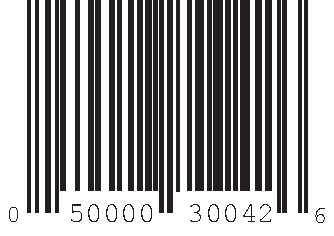
\includegraphics[width=2in]{UPCcode}
}
\end{center}
\caption{A UPC code}
\label{groups_figure_3}
\end{figure}

\item
It is often useful to use an inner product notation for this type of error detection scheme; hence, we will use the notion
\[
(d_1, d_2, \ldots, d_k ) \cdot (w_1, w_2, \ldots, w_k ) \equiv 0 \pmod{ n }
\]
to mean
\[
d_1 w_1 +  d_2 w_2 + \cdots +  d_k w_k  \equiv 0  \pmod{ n}.
\]

Suppose that $(d_1, d_2, \ldots, d_k ) \cdot (w_1, w_2, \ldots, w_k ) \equiv 0 \pmod{ n}$ is an error detection scheme for the $k$-digit identification number $d_1 d_2 \cdots d_k$, where $0 \leq d_i < n$.  Prove that all single-digit errors are detected if and only if $\gcd( w_i, n ) = 1$ for  $1 \leq i \leq k$. 

\item
Let $(d_1, d_2, \ldots, d_k ) \cdot (w_1, w_2, \ldots, w_k ) \equiv 0 \pmod{ n}$ be an error detection scheme for the $k$-digit identification number $d_1 d_2 \cdots d_k$, where $0 \leq d_i < n$.  Prove that all transposition errors of two digits $d_i$ and $d_j$ are detected if and only if $\gcd( w_i - w_j, n ) = 1$ for $i$ and  $j$ between 1 and $k$. 

\item
{\bf ISBN Codes.} 
Every book has an International Standard Book Number\index{International standard book number} (ISBN) code.  This is a 10-digit code indicating the book's publisher and title.  The tenth digit is a check digit satisfying 
\[
(d_1, d_2, \ldots, d_{10} ) \cdot (10, 9, \ldots, 1 )  \equiv 0 \pmod{11}.
\]
One problem is that $d_{10}$ might have to be a 10 to make the inner product zero; in this case, 11 digits would be  needed to make this scheme work.  Therefore, the character X is used for the eleventh digit.  So ISBN 3-540-96035-X is a valid ISBN code. 
\begin{enumerate}
 
 \item
Is ISBN 0-534-91500-0 a valid ISBN code?  What about ISBN 0-534-91700-0 and ISBN 0-534-19500-0? 
 
 \item
Does this method detect all single-digit errors?  What about all transposition errors? 
 
 \item
How many different ISBN codes are there?
 
 \item
Write a computer program that will calculate the check digit for the first nine digits of an ISBN code. 
 
 \item
A publisher has houses in Germany and the United States.  Its German prefix is 3-540.  If its United States prefix will be 0-{\it abc}, find {\it abc} such that the rest of the ISBN code will be the same for a book printed in Germany and in the United States. Under the ISBN coding method the first digit identifies the language; German is  3 and English is  0.  The next group of numbers identifies the publisher, and the last group identifies the specific book. 
 
\end{enumerate}
 
\end{enumerate}
}
 
 
 
\subsection*{References and Suggested Readings} % references need to be updated
 
 
{\small
References [2] and [3] show  how group theory can be used in error
detection schemes.  Other sources cover more advanced
topics in group theory. 
\begin{itemize}
 
\item[{\bf [1]}]
Burnside, W. {\it Theory of Groups of Finite Order}. 2nd ed. Cambridge
University Press, Cambridge, 1911; Dover, New York, 1953.  A classic. 
 
\item[{\bf [2]}]
Gallian, J. A. and Winters, S. ``Modular Arithmetic in the
Marketplace,'' {\it The American Mathematical Monthly} {\bf
95}(1988): 548--51. 
 
\item[{\bf [3]}]
Gallian, J. A. {\it Contemporary Abstract Algebra}. 2nd ed. D. C.
Heath, Lexington, MA, 1990.
 
\item[{\bf [4]}]
Hall, M. {\it Theory of Groups}. 2nd ed. Chelsea, New York, 1975.
 
\item[{\bf [5]}]
Kurosh, A. E. {\it The Theory of Groups}, vols. I and II. Chelsea, New
York, 1979. 
 
\item[{\bf [6]}]
MacDonald, I. D. {\it The Theory of Groups}. Krieger, London, 1988.
 
\item[{\bf [7]}]
Rose, J. S. {\it A Course on Group Theory}. Cambridge University
Press, Cambridge, 1978.
 
 
\item[{\bf [8]}]
Rotman, J. J. {\it An Introduction to the Theory of Groups}. 3rd ed.
Allyn and Bacon, Boston, 1984. 
 
\end{itemize}
}
 
 
 
   %Groups
\chapter{Cyclic Groups}\label{cyclic}
 
The groups $\mathbb Z$ and ${\mathbb Z}_n$, which are among the most familiar and easily understood groups, are both examples of what are called cyclic groups.  In this chapter we will study the properties of cyclic groups and cyclic subgroups, which play a fundamental part in the classification of all abelian groups. 


\section{Cyclic Subgroups}

Often a subgroup will depend entirely on a single element of the group; that is, knowing that particular element will allow us to compute any other element in the subgroup. 

\medskip

\noindent {\bf Example 1.}
Suppose that we consider $3 \in {\mathbb Z}$ and look at all multiples (both positive and negative) of 3.  As a set, this is 
$$
3 {\mathbb Z} = \{ \ldots, -3, 0, 3, 6, \ldots \}.
$$
It is easy to see that $3 {\mathbb Z}$ is a subgroup of the integers.  This subgroup is completely determined by the element 3 since we can obtain all of the other elements of the group by taking multiples of 3.  Every element in the subgroup is ``generated'' by 3. 
\hspace{\fill} $\blacksquare$

\medskip

\noindent {\bf Example 2.}
If $H = \{ 2^n : n \in {\mathbb Z} \}$, then $H$ is a subgroup of the multiplicative group of nonzero rational numbers, ${\mathbb Q}^*$.  If $a = 2^m$ and $b = 2^n$ are in $H$, then $ab^{-1} = 2^m 2^{-n} = 2^{m-n}$ is also in $H$.  By Proposition~2.10, $H$ is a subgroup of ${\mathbb Q}^*$ determined by the element 2. 
\hspace{\fill} $\blacksquare$

\begin{theorem}
Let $G$ be a group and $a$ be any element in $G$.  Then the set
$$
\langle a \rangle  = \{ a^k : k \in {\mathbb Z} \}\label{generatedby}
$$
is a subgroup of $G$.  Furthermore, $\langle a \rangle$ is the smallest subgroup of $G$ that contains~$a$. 
\end{theorem}
 
 
\begin{proof}
The identity is in $\langle a \rangle $ since $a^0 = e$. If $g$ and
$h$ are any two elements in $\langle a \rangle $, then by the
definition of $\langle a \rangle$ we can write $g = a^m$ and $h = a^n$
for some integers $m$ and $n$. So $gh = a^m a^n = a^{m+n}$ is again in
$\langle a \rangle $. Finally, if $g = a^n$ in $\langle a \rangle $,
then the inverse $g^{-1} = a^{-n}$ is also in $\langle a \rangle $.
Clearly, any subgroup $H$ of $G$ containing $a$ must contain all the
powers of $a$ by closure; hence, $H$ contains $\langle a \rangle $.
Therefore, $\langle a \rangle $ is the smallest subgroup of $G$
containing $a$. 
\end{proof}
 
 
\medskip
 
 
\noindent {\bf Remark.}
If we are using the ``+'' notation, as in the case of the integers under
addition, we write $\langle a \rangle  = \{ na : n \in {\mathbb Z} \}$.
 
 
\medskip
 
 
For $a \in G$, we call $\langle a \rangle $ the {\bfi cyclic
subgroup\/}\index{Subgroup!cyclic} generated by $a$. If $G$ contains
some element $a$ such that $G = \langle a \rangle $, then $G$ is a
{\bfi cyclic group}\index{Group!cyclic}. In this case $a$ is a {\bfi
generator\/}\index{Generator of a cyclic subgroup} of $G$.  If $a$ is an
element of a group $G$, we define the {\bfi order}\index{Element!order
of} of $a$ to be the smallest positive integer $n$ such that $a^n= e$,
and we write $|a| = n$\label{noteelementorder}. If there is no such
integer $n$, we say that the order of $a$ is infinite and  write $|a|
= \infty$ to denote the order of $a$.
 
 
\medskip
 
 
\noindent {\bf Example 3.}
Notice that a cyclic group can have more than a single
generator. Both 1 and 5 generate ${\mathbb Z}_6$; hence, ${\mathbb Z}_6$ is
a cyclic group. Not every element in a cyclic group is necessarily a
generator of the group. The order of $2 \in {\mathbb Z}_6$ is 3. The
cyclic subgroup generated by 2 is $\langle 2 \rangle  = \{ 0, 2, 4
\}$.  
\hspace{\fill} $\blacksquare$
 
 
\vspace{2ex}
 
 
The groups ${\mathbb Z}$ and ${\mathbb Z}_n$ are cyclic groups. The elements
1 and $-1$ are generators for ${\mathbb Z}$.  We can certainly generate
${\mathbb Z}_n$ with 1 although there may be other generators of ${\mathbb
Z}_n$, as in the case of ${\mathbb Z}_6$. 
 
 
\medskip
 
 
\noindent {\bf Example 4.}
The group of units, $U(9)$, in ${\mathbb Z}_9$ is a cyclic group.  As a
set, $U(9)$ is $\{ 1, 2, 4, 5, 7, 8  \}$. The element 2 is a generator
for $U(9)$ since 
$$
\begin{array}{rclccrcl}
2^1 & = & 2 & & & 2^2 & = & 4 \\
2^3 & = & 8 & & & 2^4 & = & 7 \\
2^5 & = & 5 & & & 2^6 & = & 1.
\end{array}
$$
\hspace{\fill} $\blacksquare$
 
 
\medskip
 
 
\noindent {\bf Example 5.}
Not every group is a cyclic group.  Consider the symmetry group of an
equilateral triangle $S_3$.  The multiplication table for this group
is Table~2.2. The subgroups of $S_3$ are shown in
Figure~\ref{subgrpsS3}.  Notice that every subgroup is cyclic;
however, no single element generates the entire group.
\mbox{\hspace{1in}}
\hspace{\fill} $\blacksquare$
 
 
\begin{figure}[htb]
\begin{center}
\setlength{\unitlength}{.2in}
\begin{picture}(18,9)(-2,1)
\put(7.3,8.6){$S_3$}
\put(7,1){$\{ id \}$}
\put(-1,5){$\{id, \rho_1, \rho_2  \}$}
\put(3.8,5){$\{id, \mu_1 \}$}
\put(9,5){$\{id, \mu_2 \}$}
\put(13,5){$\{id, \mu_3 \}$}
\put(1,6){\line(5,2){5}}
\put(1,4){\line(5,-2){5}}
\put(5,6){\line(3,4){1.5}}
\put(5,4){\line(3,-4){1.5}}
\put(10,6){\line(-3,4){1.5}}
\put(10,4){\line(-3,-4){1.5}}
\put(14,6){\line(-5,2){5}}
\put(14,4){\line(-5,-2){5}}
\end{picture}
\end{center}
\caption{Subgroups of $S_3$}
\label{subgrpsS3}
\end{figure}
 
 
\begin{theorem}
Every cyclic group is abelian.
\end{theorem}
 
 
\begin{proof}
Let $G$ be a cyclic group and $a \in G$ be a generator for $G$. If
$g$ and $h$ are in $G$, then they can be written as powers of $a$,
say $g = a^r$ and $h = a^s$. Since
$$
g  h = a^r a^s = a^{r+s} = a^{s+r} = a^s a^r = h g,
$$
$G$ is abelian.
\end{proof}
 
 
 
\subsection*{Subgroups of Cyclic Groups}
 
 
We can ask some interesting questions about cyclic subgroups of a
group and subgroups of a cyclic group.  If $G$ is a group, which
subgroups of $G$ are cyclic? If $G$ is a cyclic group, what type of
subgroups does $G$ possess? 
 
 
 
\begin{theorem}
Every subgroup of a cyclic group is cyclic.
\end{theorem}
 
 
\begin{proof}
The main tools used in this proof are the division algorithm and the
Principle of Well-Ordering. Let $G$ be a cyclic group generated by $a$
and suppose that $H$ is a subgroup of $G$. If $H = \{ e \}$, then
trivially $H$ is cyclic. Suppose that $H$ contains some other element
$g$ distinct from the identity. Then $g$ can be written as
$a^n$ for some integer $n$. We can assume that $n > 0$. Let $m$ be the
smallest natural number such that $a^m \in H$. Such an $m$ exists by
the Principle of Well-Ordering.
 
 
We claim that $h = a^m$ is a generator for $H$.  We must show that
every $h' \in H$ can be written as a power of $h$. Since $h' \in H$
and $H$ is a subgroup of $G$, $h' = a^k$ for some positive integer
$k$. Using the division algorithm, we can find numbers $q$ and $r$
such that $k = mq +r$ where $0 \leq r < m$; hence,
$$
a^k = a^{mq +r} = (a^m)^q a^r = h^q a^r.
$$
So $a^r = a^k h^{-q}$. Since $a^k$ and $h^{-q}$ are in $H$, $a^r$ must
also be in $H$.  However, $m$ was the smallest positive number such that
$a^m$ was in $H$; consequently, $r=0$ and so $k=mq$. Therefore, 
$$
h' = a^k = a^{mq} =  h^q
$$
and $H$ is generated by $h$.
\end{proof}
 
 
\begin{corollary}
The subgroups of ${\mathbb Z}$ are exactly $n{\mathbb Z}$ for $n = 0, 1, 2,
\ldots$. 
\end{corollary}
 
 
\begin{proposition}
Let $G$ be a cyclic group of order $n$ and suppose that $a$ is a
generator for  $G$. Then $a^k=e$ if and only if $n$ divides $k$.
\end{proposition}
 
 
\begin{proof}
First suppose that $a^k=e$. By the division algorithm, $k = nq + r$
where $0 \leq r < n$; hence, 
$$
e = a^k = a^{nq + r} = a^{nq} a^r = e a^r = a^r.
$$
Since the smallest positive integer $m$ such that $a^m = e$ is $n$, $r
= 0$.
 
 
Conversely, if $n$ divides $k$, then $k=ns$ for some integer $s$.
Consequently, 
$$
a^k = a^{ns} = (a^n)^s = e^s = e.
$$
\end{proof}
 
 
\begin{theorem}
Let $G$ be a cyclic group of order $n$ and suppose that $a \in G$ is a
generator of the group.  If $b = a^k$, then the order of $b$ is $n
/d$, where $d = \gcd(k,n)$. 
\end{theorem}
 
 
\begin{proof}
We wish to find the smallest integer $m$ such that $e = b^m = a^{km}$.
By Proposition~3.5, this is the smallest integer $m$ such that
$n$ divides $km$ or, equivalently, $n/d$ divides $m(k/d)$.  Since $d$ is
the greatest common divisor of $n$ and $k$, $n/d$ and $k/d$ are
relatively prime. Hence, for $n/d$ to divide $m(k/d)$ it must divide
$m$.  The smallest such $m$ is $n/d$. 
\end{proof}
 
 
\begin{corollary}
The generators of ${\mathbb Z}_n$ are the integers $r$ such that $1 \leq
r < n$ and $\gcd(r,n) =  1$. 
\end{corollary}
 
 
\noindent {\bf Example 6.}
Let us examine the group ${\mathbb Z}_{16}$.  The numbers 1, 3, 5, 7, 9,
11, 13, and 15 are the elements of ${\mathbb Z}_{16}$ that are relatively
prime to 16.  Each of these elements generates ${\mathbb Z}_{16}$. For
example, 
$$
\begin{array}{rclccrclccrcl}
1 \cdot 9  & = & 9  &&& 2 \cdot 9  & = & 2  &&&	3 \cdot 9  & = & 11 \\
4 \cdot 9  & = & 4  &&& 5 \cdot 9  & = & 13 &&&	6 \cdot 9  & = & 6  \\
7 \cdot 9  & = & 15 &&& 8 \cdot 9  & = & 8  &&&	9 \cdot 9  & = & 1  \\
10 \cdot 9 & = & 10 &&& 11 \cdot 9 & = & 3  &&&	12 \cdot 9 & = & 12 \\
13 \cdot 9 & = & 5  &&& 14 \cdot 9 & = & 14 &&&	15 \cdot 9 & = & 7.
\end{array}
$$
\hspace{\fill} $\blacksquare$
 
 
\section{The Group ${\mathbb C}^\ast$}
 
 
The {\bfi complex numbers} are defined as
$$
{\mathbb C} = \{ a + bi : a, b \in {\mathbb R} \},
$$
where $i^2 = -1$.  If $z=a+bi$, then $a$ is the {\bfi real part} of $z$
and $b$ is the {\bfi imaginary part} of $z$. 
 
 
To add two complex numbers $z=a+bi$ and $w= c+di$, we just
add the corresponding real and imaginary parts:
$$
z+w=(a + bi ) + (c + di)  =  (a+c) + (b+d)i.
$$
Remembering that $i^2 = -1$,  we multiply complex numbers just like
polynomials. The product of $z$ and $w$ is 
$$
(a + bi )(c + di)  =   ac + bdi^2 + adi + bci =  (ac -bd) +
(ad + bc)i.
$$
 
 
Every nonzero complex number $z = a +bi$ has a multiplicative inverse;
that is, there exists a $z^{-1} \in {\mathbb C}^\ast$ such that $z z^{-1}
= z^{-1} z = 1$. If $z = a + bi$, then 
$$
z^{-1} = \frac{a-bi}{ a^2 + b^2  }.
$$
The {\bfi complex conjugate}\index{Conjugate, complex} of a complex
number $z = a +bi$ is defined to be $\overline{z} = a-bi$.  The {\bfi
absolute value} or {\bfi modulus} of  $z = a +bi$  is $|z| =
\sqrt{a^2+b^2}$.  
 
 
\vspace{ 2ex }
 
 
\noindent {\bf Example 7.}
Let $z = 2 + 3i$ and $w = 1-2i$. Then
$$
z + w = (2 + 3i)+( 1-2i ) = 3 +i
$$
and
$$
z  w = (2 + 3i)( 1-2i ) = 8-i.
$$
Also,
\begin{eqnarray*}
z^{-1} & = & \frac{2}{13} - \frac{3}{13}i \\
|z| & = & \sqrt{13} \\
\overline{z} & = & 2-3i.
\end{eqnarray*}
\hspace{\fill} $\blacksquare$
 
\vspace{ 2ex }
 
\begin{figure}[hbt]
\begin{center}
\centerline {
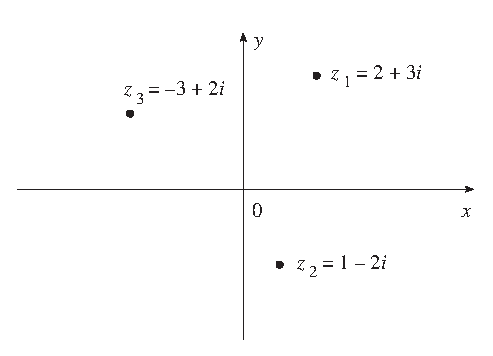
\includegraphics[width=2in]{rectcoord}
}
\end{center}
\caption{Rectangular coordinates of a complex number}
\label{rectcoord}
\end{figure}
 
 
There are several ways of graphically representing complex numbers. We
can represent a complex number $z = a +bi$ as an ordered pair on the
$xy$ plane where $a$ is the $x$ (or real) coordinate and $b$ is the $y$
(or imaginary) coordinate. This is called the {\bfi rectangular} or
{\bfi Cartesian} representation. The rectangular representations of
$z_1 = 2 + 3i$, $z_2 = 1 - 2i$, and $z_3 = - 3 + 2i$ are depicted in
Figure~\ref{rectcoord}.
 
 
\begin{figure}[htb]
\begin{center}
\centerline {
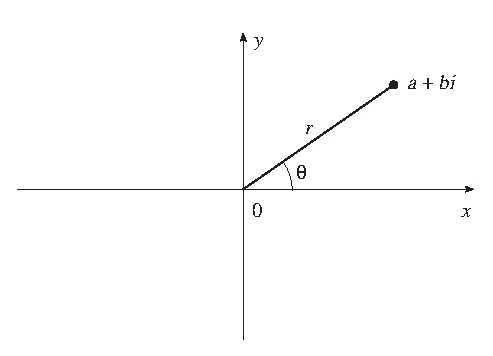
\includegraphics[width=2in]{polarcoord}
}
\end{center}
\caption{Polar coordinates of a complex number}
\label{polarcoord}
\end{figure}
 
 
Nonzero complex numbers can also be represented using {\bfi polar
coordinates}.  To specify  any nonzero point on the plane, it suffices
to give an angle $\theta$ from the positive $x$ axis in the
counterclockwise direction and a distance $r$ from the origin, as in 
Figure~\ref{polarcoord}. We can see that 
$$
z = a + bi = r( \cos \theta + i \sin \theta).
$$
Hence,
$$
r = |z| = \sqrt{a^2+b^2}
$$
and
\begin{eqnarray*}
a & = & r \cos \theta \\
b & = & r \sin \theta.
\end{eqnarray*}
We sometimes abbreviate $r( \cos \theta + i \sin \theta)$ as $r \cis
\theta$\label{cosisin}.  To assure that the representation of $z$ is 
well-defined, we also require that $0^{\circ} \leq \theta <
360^{\circ}$.  If the measurement is in radians, then $0 \leq \theta <
2 \pi$. 
 
 
\vspace{ 2ex }
 
 
\noindent {\bf Example 8.}
Suppose that $z = 2 \cis  60^{\circ}$. Then
$$
a  =  2 \cos 60^{\circ}  =   1
$$
and
$$
b  =  2 \sin 60^{\circ}  =  \sqrt{3}.
$$
Hence, the rectangular representation is $z = 1+\sqrt{3}\, i$.
 
 
Conversely, if we are given a rectangular representation of a complex
number, it is often useful to know the number's polar representation.
If $z = 3 \sqrt{2} - 3 \sqrt{2}\, i$, then 
$$
r = \sqrt{a^2 + b^2} = \sqrt{36 } = 6
$$
and
$$
\theta = \arctan \left( \frac{b}{a} \right) = \arctan( - 1) =
315^{\circ},
$$
so $3 \sqrt{2} - 3 \sqrt{2}\, i=6 \cis  315^{\circ}$.
\hspace{\fill} $\blacksquare$
 
 
\vspace{ 2ex }
 
 
The polar representation of a complex number makes it easy to find
products and powers of complex numbers.  The proof of the following
proposition is straightforward and is left as an exercise.
 
 
\begin{proposition}
Let $z = r \cis \theta$ and $w = s \cis \phi$
be two nonzero complex numbers. Then 
$$
zw = r s \cis( \theta + \phi).
$$
\end{proposition}
 
 
\noindent {\bf Example 9.}
If $z =  3 \cis( \pi / 3 )$ and $w = 2 \cis(\pi / 6 )$, then $zw = 6
\cis( \pi / 2 ) = 6i$.  
\hspace{\fill} $\blacksquare$
 
 
\begin{theorem}[DeMoivre]\index{DeMoivre's Theorem}
Let $z = r \cis  \theta$ be a nonzero complex number. Then 
$$
[r \cis \theta  ]^n
=
r^n \cis( n \theta)
$$
for $n = 1, 2, \ldots$.
\end{theorem}
 
 
\begin{proof}
We will use induction on $n$. For $n = 1$ the theorem is trivial.
Assume that the theorem is true for all $k$ such that $1  \leq k \leq
n$. Then 
\begin{eqnarray*}
z^{n+1} & = & z^n z \\
& = &
r^n( \cos  n \theta + i \sin n \theta ) r( \cos \theta + i
\sin \theta ) \\
& = &
r^{n+1} [( \cos n \theta \cos \theta - \sin n \theta \sin
\theta )
 + i ( \sin n \theta \cos \theta + \cos n \theta \sin \theta
)] \\
& = &
r^{n+1} [ \cos( n \theta + \theta) + i \sin( n \theta +
\theta) ] \\
& = &
r^{n+1} [ \cos( n +1) \theta + i \sin( n+1) \theta  ].
\end{eqnarray*}
\end{proof}
 
 
\vspace{2ex}
 
 
\noindent {\bf Example 10.}
Suppose that $z= 1+i$ and we wish to compute $z^{10}$. Rather than
computing $(1+i)^{10}$ directly, it is much easier to switch to polar
coordinates and calculate $z^{10}$ using DeMoivre's Theorem:
\begin{eqnarray*}
z^{10}
& = &
(1+i)^{10} \\
& = &
\left( \sqrt{2} \cis \left( \frac{\pi }{4} \right)
\right)^{10} \\
& = &
( \sqrt{2}\, )^{10} \cis \left( \frac{5\pi }{2} \right)
\\
& = &
32  \cis \left( \frac{\pi }{2} \right) \\
& = & 32i.
\end{eqnarray*}
\hspace{\fill} $\blacksquare$
 
 
\subsection*{The Circle Group and the Roots of Unity }
 
 
The multiplicative group of the complex numbers, ${\mathbb C}^*$,
possesses some interesting subgroups.  Whereas ${\mathbb Q}^*$ and ${\mathbb
R}^*$ have no interesting subgroups of finite order, ${\mathbb C}^*$ has 
many. We first consider the {\bfi circle group}\index{Group!circle}, 
$$
{\mathbb T}\label{notecirclegroup} = \{ z \in {\mathbb C} : |z| = 1 \}.
$$
The following proposition is a direct result of Proposition~3.8.
 
 
\begin{proposition}
The circle group is a subgroup of  ${\mathbb C}^*$.
\end{proposition}
 
 
Although the circle group has infinite order, it has many interesting 
finite subgroups. Suppose that $H = \{ 1, -1, i, -i \}$. Then $H$ is a
subgroup of the circle group. Also, $1$, $-1$, $i$, and $-i$ are
exactly those complex numbers that satisfy the equation $z^4=1$. 
The complex numbers satisfying the equation $z^n=1$ are called
the {\bfi nth roots of unity}\index{$n$th root of unity}. 
 
 
\begin{theorem}
If $z^n = 1$, then the $n$th roots of unity are
$$
z = \cis \left( \frac{2 k \pi}{n } \right),
$$
where $k = 0, 1, \ldots, n-1$. Furthermore, the $n$th roots of unity
form a cyclic subgroup of\/ ${\mathbb T}$ of order $n$. 
\end{theorem}
 
 
\begin{proof}
By DeMoivre's Theorem,
$$
z^n = \cis \left( n \frac{2 k \pi}{n } \right) =
\cis( 2 k \pi ) = 1.
$$
The $z$'s are distinct since the numbers $2 k \pi /n$ are all
distinct and are greater than or equal to 0 but less than $2 \pi$.
The fact that these are all of the roots of the equation $z^n=1$
follows from the Fundamental Theorem of Algebra (Theorem~19.16), which
states that a polynomial of degree $n$ can have at most $n$ roots.  We
will leave the proof that the $n$th roots of unity form a cyclic
subgroup of ${\mathbb T}$ as an exercise.
\end{proof}
 
 
\vspace{2ex}
 
 
A generator for the group of the $n$th roots of unity is called a
{\bfi primitive nth root of unity}\index{Primitive $n$th root of
unity}. 
 
 
\vspace{2ex}
 
 
\noindent {\bf Example 11.}
The 8th roots of unity can be represented as
eight equally spaced points on the unit circle (Figure~\ref{rtsunity}).  The
primitive 8th roots of unity are
\begin{eqnarray*}
\omega & = & \frac{\sqrt{2}}{2}  + \frac{\sqrt{2}}{2} i \\
\omega^3 & = & -\frac{\sqrt{2}}{2}  + \frac{\sqrt{2}}{2} i \\
\omega^5 & = & -\frac{\sqrt{2}}{2}  - \frac{\sqrt{2}}{2} i \\
\omega^7 & = & \frac{\sqrt{2}}{2}  - \frac{\sqrt{2}}{2}i. 
\end{eqnarray*}
\hspace{\fill} $\blacksquare$
 
 
 
\begin{figure}[hbt]
\begin{center}
\centerline {
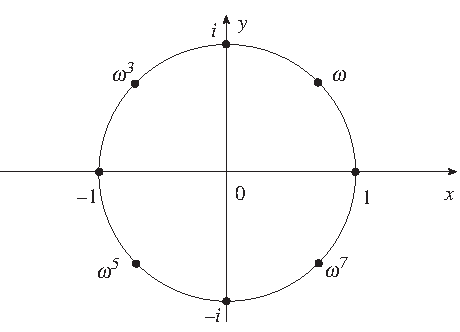
\includegraphics[width=2in]{rtsunity}
}
\end{center}
\caption{8th roots of unity}
\label{rtsunity}
\end{figure}
 
 
 
 
\section[The Method of Repeated Squares]{The Method of Repeated
Squares\protect\footnotemark}\index{Repeated squares} 
\footnotetext{The results in this section are needed only in
Chapter~6.}   
 
 
Computing large powers can be very time-consuming. Just as anyone can
compute $2^2$ or $2^8$, everyone knows how to compute
$$
2^{2^{1000000} }.
$$
However, such numbers are so large that we do not want to attempt the
calculations; moreover,past a certain point the computations would not
be feasible even if we had every computer in the world at our
disposal. Even 
writing down the decimal representation of a very large number may not
be reasonable. It could be thousands or even millions of digits long.
However, if we could compute something like $2^{37398332 } \pmod{
46389}$, we could very easily write the result down since it would be a
number between 0 and 46,388. If we want to compute powers modulo $n$
quickly and efficiently, we will have to be clever. 
 
 
The first thing to notice is that any number $a$ can be written as the
sum of distinct powers of 2; that is, we can write
$$
a = 2^{k_1} + 2^{k_2} + \cdots + 2^{k_n},
$$
where $k_1 < k_2 < \cdots < k_n$.  This is just the binary
representation of $a$. For example, the binary representation of 57 is
111001, since we can write $57 = 2^0 + 2^3 + 2^4 + 2^5$.
 
 
The laws of exponents still work in ${\mathbb Z}_n$; that is, if $b
\equiv a^x \pmod{ n}$ and $c \equiv a^y \pmod{ n}$, then $bc \equiv
a^{x+y} \pmod{ n}$. We can compute $a^{2^k} \pmod{ n}$ in $k$
multiplications by computing 
$$
\begin{array}{c}
a^{2^0} \pmod{ n} \\
a^{2^1} \pmod{ n }\\
\vdots \\
a^{2^k} \pmod{ n}.
\end{array}
$$
Each step involves squaring the answer obtained in the previous step,
dividing by $n$, and taking the remainder.
 
 
\medskip
 
 
\noindent {\bf Example 12.}
We will compute $271^{321} \pmod{ 481}$. Notice that
$$
321 = 2^0 +2^6 + 2^8;
$$
hence, computing $271^{ 321} \pmod{ 481}$ is the same as computing
$$
271^{ 2^0 +2^6 + 2^8 } \equiv 271^{ 2^0 } \cdot 271^{
2^6 } \cdot 271^{ 2^8 } \pmod{ 481}.
$$
So it will suffice to compute $271^{ 2^i } \pmod{ 481}$ where $i = 0,
6, 8$. It is very easy to see that 
\begin{eqnarray*}
271^{ 2^1}  & \equiv & 73,441 \pmod{ 481}  \\
& \equiv & 329 \pmod{ 481}.
\end{eqnarray*}
We can square this result to obtain a value for $271^{ 2^2} \pmod{
481}$: 
\begin{eqnarray*}
271^{ 2^2}  & \equiv & (271^{ 2^1})^2 \pmod{ 481}
\\ & \equiv & (329)^2 \pmod{ 481} \\
& \equiv & 1,082,411 \pmod{ 481} \\
& \equiv & 16 \pmod{ 481}.
\end{eqnarray*}
We are using the fact that $(a^{2^n})^2  \equiv a^{2 \cdot 2^n} \equiv
a^{ 2^{n+1} } \pmod{ n}$. Continuing, we can calculate
$$
271^{ 2^6 } \equiv 419 \pmod{ 481}
$$
and
$$
271^{ 2^8 }  \equiv 16 \pmod{ 481}.
$$
Therefore,
\begin{eqnarray*}
271^{ 321}
& \equiv & 271^{ 2^0 +2^6 + 2^8 } \pmod{ 481} \\
& \equiv & 271^{ 2^0 } \cdot 271^{ 2^6 } \cdot 271^{ 2^8 }
\pmod{ 481} \\
& \equiv & 271 \cdot 419 \cdot 16 \pmod{ 481} \\
& \equiv & 1,816,784 \pmod{ 481} \\
& \equiv & 47 \pmod{ 481}.
\end{eqnarray*}
\hspace{\fill} $\blacksquare$
 
 
The method of repeated squares will prove to be a very useful tool
when we explore  RSA cryptography  in Chapter~6. To encode and decode
messages in a reasonable manner under this scheme, it is necessary to
be able to quickly compute large powers of integers mod $n$.
 
 
\markright{EXERCISES}
\section*{Exercises}
\exrule
 
 
 
 
{\small
\begin{enumerate}
 
 
\bf\item\rm
Prove or disprove each of the following statements.
\begin{enumerate}
 
 \bf\item\rm
$U(8)$ is cyclic.
 
 \bf\item\rm
All of the generators of ${\mathbb Z}_{60}$ are prime.
 
 \bf\item\rm
${\mathbb Q}$ is cyclic.
 
 \bf\item\rm
If every subgroup of a group $G$ is cyclic, then $G$ is a cyclic
group. 
 
 \bf\item\rm
A group with a finite number of subgroups is finite.
 
\end{enumerate}
 
 
\bf\item\rm
Find the order of each of the following elements.
 
 
\vspace{3pt}        %two column exercise list
 
\hspace{-7pt}
\begin{minipage}[t]{4.6in}
\noindent
\begin{minipage}[t]{2.25in}
\begin{itemize}
 
 \item[{\bf (a)}]
$5 \in {\mathbb Z}_{12}$
 
 \item[{\bf (c)}]
$\sqrt{3} \in {\mathbb R}^\ast$
 
 \item[{\bf (e)}]
72 in ${\mathbb Z}_{240}$
 
\end{itemize}
\end{minipage} \hfill
\begin{minipage}[t]{2.25in}
\begin{itemize}
 
 \item[{\bf (b)}]
$\sqrt{3} \in {\mathbb R}$
 
 \item[{\bf (d)}]
$-i \in {\mathbb C}^\ast$
 
 \item[{\bf (f)}]
312 in ${\mathbb Z}_{471}$
 
\end{itemize}
\end{minipage}
\end{minipage}
 
\vspace{2pt}        %end two column exercise list
 
 
\bf\item\rm
List all of the elements in each of the following subgroups.
\begin{enumerate}
 
 \bf\item\rm
The subgroup of ${\mathbb Z}$ generated by 7
 
 \bf\item\rm
The subgroup of ${\mathbb Z}_{24}$ generated by 15
 
 \bf\item\rm
All subgroups of ${\mathbb Z}_{12}$
 
 \bf\item\rm
All subgroups of ${\mathbb Z}_{60}$
 
 \bf\item\rm
All subgroups of ${\mathbb Z}_{13}$
 
 \bf\item\rm
All subgroups of ${\mathbb Z}_{48}$
 
 \bf\item\rm
The subgroup generated by 3  in $U(20)$
 
 \bf\item\rm
The subgroup generated by 6  in $U(18)$
 
 \bf\item\rm
The subgroup of ${\mathbb R}^\ast$ generated by 7
 
 \bf\item\rm
The subgroup of ${\mathbb C}^\ast$ generated by $i$ where $i^2 = -1$
 
 \bf\item\rm
The subgroup of ${\mathbb C}^\ast$ generated by $2i$
 
 \bf\item\rm
The subgroup of ${\mathbb C}^\ast$ generated by $(1 + i) / \sqrt{2}$
 
 \bf\item\rm
The subgroup of ${\mathbb C}^\ast$ generated by $(1 + \sqrt{3}\, i) / 2$
 
\end{enumerate}
 
 
\bf\item\rm
Find the subgroups of $GL_2( {\mathbb R })$ generated by each of the
following matrices. 
 
 
\vspace{3pt}        %two column exercise list
 
\hspace{-7pt}
\begin{minipage}[t]{4.6in}
\noindent
\begin{minipage}[t]{2.25in}
\begin{itemize}
 
 \item[{\bf (a)}]
\raisebox{-5.25pt}{\parbox{1.85in}{
$$
\left(
\begin{array}{cc}
0 & 1 \\
-1 & 0
\end{array}
\right)
$$
}}
 
 \item[{\bf (c)}]
\raisebox{-5.25pt}{\parbox{1.85in}{
$$
\left(
\begin{array}{cc}
1 & -1 \\
1 & 0
\end{array}
\right)
$$
}}
 
 \item[{\bf (e)}]
\raisebox{-5.25pt}{\parbox{1.85in}{
$$
\left(
\begin{array}{cc}
1 & -1 \\
-1 & 0
\end{array}
\right)
$$
}}
 
\end{itemize}
\end{minipage} \hfill
\begin{minipage}[t]{2.25in}
\begin{itemize}
 
 \item[{\bf (b)}]
\raisebox{-5.25pt}{\parbox{1.85in}{
$$
\left(
\begin{array}{cc}
0 & 1/3 \\
3 & 0
\end{array}
\right)
$$
}}
 
 \item[{\bf (d)}]
\raisebox{-5.25pt}{\parbox{1.85in}{
$$
\left(
\begin{array}{cc}
1 & -1 \\
0 & 1
\end{array}
\right)
$$
}}
 
 \item[{\bf (f)}]
\raisebox{-5.25pt}{\parbox{1.85in}{
$$
\left(
\begin{array}{cc}
\sqrt{3}/ 2 & 1/2 \\
-1/2 & \sqrt{3}/2
\end{array}
\right)
$$
}}
 
\end{itemize}
\end{minipage}
\end{minipage}
 
\vspace{2pt}        %end two column exercise list
 
 
\bf\item\rm		  %%%%%%%%%%%%%%%%%%%%%%%%
Find the order of every element in ${\mathbb Z}_{18}$.
 
 
\bf\item\rm
Find the order of every element in the symmetry group of the square,
$D_4$.
 
 
\bf\item\rm
What are all of the cyclic subgroups of the quaternion group, $Q_8$? 
 
 
\bf\item\rm
List all of the cyclic subgroups of $U(30)$.
 
 
\bf\item\rm
List every generator of each subgroup of order 8 in ${\mathbb
Z}_{32}$.
 
 
\bf\item\rm
Find all elements of finite order in each of the following groups. 
\begin{enumerate}
 
 \bf\item\rm
${\mathbb Z}$
 
 \bf\item\rm
${\mathbb Q}^\ast$
 
 \bf\item\rm
${\mathbb R}^\ast$
 
\end{enumerate}
 
 
\bf\item\rm
If $a^{24} =e$ in a group $G$, what are the possible orders of $a$? 
 
 
\bf\item\rm
Find a cyclic group with exactly one generator.  Can you find cyclic
groups with exactly two generators?  Four generators?  How about $n$
generators?
 
 
\bf\item\rm
For $n \leq 20$, which groups $U(n)$ are cyclic?  Make a conjecture as
to what is true in general.  Can you prove your conjecture?  
 
 
\bf\item\rm
Let
$$
A=
\left(
\begin{array}{cc}
0 & 1 \\
-1 & 0
\end{array}
\right)
$$
and
$$
B=
\left(
\begin{array}{cc}
0 & -1 \\
1 & -1
\end{array}
\right)
$$
be elements in $GL_2( {\mathbb R} )$. Show that $A$ and $B$ have finite
orders but $AB$ does not. 
 
 
\bf\item\rm
Evaluate each of the following.
 
 
\vspace{3pt}        %two column exercise list
 
\hspace{-7pt}
\begin{minipage}[t]{4.6in}
\noindent
\begin{minipage}[t]{2.25in}
\begin{itemize}
 
 \item[{\bf (a)}]
$(3-2i)+ (5i-6)$
 
 \item[{\bf (c)}]
$(5-4i)(7+2i)$
 
 \item[{\bf (e)}]
$i^{45}$
 
\end{itemize}
\end{minipage} \hfill
\begin{minipage}[t]{2.25in}
\begin{itemize}
 
 \item[{\bf (b)}]
 $(4-5i)-\overline{(4i -4)}$
 
 \item[{\bf (d)}]
$(9-i) \overline{(9-i)}$
 
 \item[{\bf (f)}]
$(1+i)+\overline{(1+i)}$
 
\end{itemize}
\end{minipage}
\end{minipage}
 
\vspace{2pt}        %end two column exercise list
 
 
\bf\item\rm   %%%%%%%%%%%%%%%%%%%%%%%%
Convert the following complex numbers to the form $a + bi$.
 
 
\vspace{3pt}        %two column exercise list
 
\hspace{-7pt}
\begin{minipage}[t]{4.6in}
\noindent
\begin{minipage}[t]{2.25in}
\begin{itemize}
 
 \item[{\bf (a)}]
$2 \cis(\pi / 6 )$
 
 \item[{\bf (c)}]
$3 \cis(\pi)$
 
\end{itemize}
\end{minipage} \hfill
\begin{minipage}[t]{2.25in}
\begin{itemize}
 
 \item[{\bf (b)}]
$5 \cis(9\pi/4)$
 
 \item[{\bf (d)}]
$\cis(7\pi/4) /2$
 
\end{itemize}
\end{minipage}
\end{minipage}
 
\vspace{2pt}        %end two column exercise list
 
 
\bf\item\rm	  %%%%%%%%%%%%%%%%%%%%%%%%%%%%%%%%
Change the following complex numbers to polar representation.
 
 
\vspace{3pt}        %two column exercise list
 
\hspace{-7pt}
\begin{minipage}[t]{4.6in}
\noindent
\begin{minipage}[t]{2.25in}
\begin{itemize}
 
 \item[{\bf (a)}]
$1-i$
 
 \item[{\bf (c)}]
$2+2i$
 
 \item[{\bf (e)}]
$-3i$
 
\end{itemize}
\end{minipage} \hfill
\begin{minipage}[t]{2.25in}
\begin{itemize}
 
 \item[{\bf (b)}]
$-5$
 
 \item[{\bf (d)}]
$\sqrt{3} + i$
 
 \item[{\bf (f)}]
$2i + 2 \sqrt{3}$
 
\end{itemize}
\end{minipage}
\end{minipage}
 
\vspace{2pt}        %end two column exercise list
 
 
\bf\item\rm %%%%%%%%%%%%%%%%%%%%%%%%
Calculate each of the following expressions.
 
 
\vspace{3pt}        %two column exercise list
 
\hspace{-7pt}
\begin{minipage}[t]{4.6in}
\noindent
\begin{minipage}[t]{2.25in}
\begin{itemize}
 
 \item[{\bf (a)}]
$(1+i)^{-1}$
 
 \item[{\bf (c)}]
$(\sqrt{3}+i)^{5}$
 
 \item[{\bf (e)}]
$((1-i)/2)^{4}$
 
 \item[{\bf (g)}]
$(-2+2i)^{-5}$
 
\end{itemize}
\end{minipage} \hfill
\begin{minipage}[t]{2.25in}
\begin{itemize}
 
 \item[{\bf (b)}]
$(1-i)^{6}$
 
 \item[{\bf (d)}]
$(-i)^{10}$
 
 \item[{\bf (f)}]
$(-\sqrt{2} - \sqrt{2}\, i)^{12}$
 
\end{itemize}
\end{minipage}
\end{minipage}
 
\vspace{2pt}        %end two column exercise list
 
 
 
\bf\item\rm
Prove each of the following statements.
 
 
\vspace{3pt}        %two column exercise list
 
\hspace{-7pt}
\begin{minipage}[t]{4.6in}
\noindent
\begin{minipage}[t]{2.25in}
\begin{itemize}
 
 \item[{\bf (a)}]
$|z| = | \overline{z}|$
 
 
 \item[{\bf (c)}]
$z^{-1} = \overline{z} / |z|^2$
 
 \item[{\bf (e)}]
$|z - w| \geq | |z| - |w||$
 
\end{itemize}
\end{minipage} \hfill
\begin{minipage}[t]{2.25in}
\begin{itemize}
 
 \item[{\bf (b)}]
$z \overline{z} = |z|^2$
 
 \item[{\bf (d)}]
$|z +w| \leq |z| + |w|$
 
 \item[{\bf (f)}]
$|z w| = |z|  |w|$
 
\end{itemize}
\end{minipage}
\end{minipage}
 
\vspace{2pt}        %end two column exercise list
 
 
\bf\item\rm
List and graph the 6th roots of unity.  What are the generators of
this group?  What are the primitive 6th roots of unity?
 
 
\bf\item\rm
List and graph the 5th roots of unity.  What are the generators of
this group?  What are the primitive 5th roots of unity? 
 
 
\bf\item\rm
Calculate each of the following.
 
 
\vspace{3pt}        %two column exercise list
 
\hspace{-7pt}
\begin{minipage}[t]{4.6in}
\noindent
\begin{minipage}[t]{2.25in}
\begin{itemize}
 
 \item[{\bf (a)}]
$292^{3171} \pmod{ 582}$
 
 \item[{\bf (c)}]
$2071^{ 9521} \pmod{ 4724}$
 
\end{itemize}
\end{minipage} \hfill
\begin{minipage}[t]{2.25in}
\begin{itemize}
 
 \item[{\bf (b)}]
$2557^{ 341} \pmod{ 5681}$
 
 \item[{\bf (d)}]
$971^{ 321} \pmod{ 765}$
 
\end{itemize}
\end{minipage}
\end{minipage}
 
\vspace{2pt}        %end two column exercise list
 
 
 
\bf\item\rm
Let $a, b \in G$.  Prove the following statements.
\begin{enumerate}
 
 \bf\item\rm
The order of $a$ is the same as the order of $a^{-1}$.
 
 \bf\item\rm
For all $g \in G$, $|a| = |g^{-1}ag|$.
 
 \bf\item\rm
The order of $ab$ is the same as the order of $ba$.
 
\end{enumerate}
 
 
\bf\item\rm
Let $p$ and $q$ be distinct primes.  How many generators does ${\mathbb
Z}_{pq}$ have? 
 
 
\bf\item\rm
Let $p$ be prime and $r$ be a positive integer.  How many generators
does ${\mathbb Z}_{p^r}$ have? 
 
 
\bf\item\rm
Prove that  ${\mathbb Z}_{p}$ has no nontrivial subgroups if $p$ is
prime. 
 
 
\bf\item\rm
If $g$ and $h$ have orders 15 and 16 respectively in a group $G$, what
is the order of $\langle g \rangle  \cap \langle h \rangle $? 
 
 
\bf\item\rm
Let $a$ be an element in a group $G$. What is a generator for the
subgroup $\langle a^m \rangle  \cap  \langle a^n \rangle $?
 
 
\bf\item\rm
Prove that ${\mathbb Z}_n$ has an even number of generators for $n>2$. 
 
 
\bf\item\rm
Suppose that $G$ is a group and let $a$, $b \in G$. Prove that if $|a|
= m$ and $|b| = n$ with $\gcd(m,n) = 1$, then $\langle a \rangle  \cap
\langle b \rangle  = \{ e \}$. 
 
 
\bf\item\rm
Let $G$ be an abelian group. Show that the elements of finite order in
$G$ form a subgroup. This subgroup is called the {\bfi torsion
subgroup}\index{Subgroup!torsion} of $G$. 
 
 
\bf\item\rm
Let $G$ be a finite cyclic group of order $n$ generated by $x$. Show
that if $y = x^k$ where $\gcd(k,n) = 1$, then $y$ must be a generator
of $G$.
 
 
\bf\item\rm
If $G$ is an abelian group that contains a pair of cyclic subgroups of
order 2, show that $G$ must contain a subgroup of order 4. Does this
subgroup have to be cyclic?
 
 
\bf\item\rm
Let $G$ be an abelian group of order $pq$ where $\gcd(p,q) = 1$.  If
$G$ contains elements $a$ and $b$ of order $p$ and $q$ respectively,
then show that $G$ is cyclic. 
 
 
\bf\item\rm
Prove that the subgroups of ${\mathbb Z}$ are exactly $n{\mathbb Z}$ for $n
= 0, 1, 2, \ldots$. 
 
 
\bf\item\rm
Prove that the generators of ${\mathbb Z}_n$ are the integers $r$ such
that $1 \leq r < n$ and $\gcd(r,n) =  1$. 
 
 
\bf\item\rm
Prove that if $G$ has no proper nontrivial subgroups, then $G$ is a 
cyclic group.
 
 
 
\bf\item\rm
Prove that the order of an element in a cyclic group $G$ must divide
the order of the  group. 
 
 
\bf\item\rm
For what integers $n$ is $-1$ an $n$th root of unity?
 
 
\bf\item\rm
If $z = r( \cos \theta + i \sin \theta)$ and $w = s(\cos \phi + i \sin
\phi)$ are two nonzero complex numbers, show that
$$
zw = rs[ \cos( \theta + \phi)  + i \sin( \theta + \phi)].
$$
 
 
\bf\item\rm
Prove that the circle group is a subgroup of  ${\mathbb C}^*$.
 
 
\bf\item\rm
Prove that the $n$th roots of unity form a cyclic subgroup of ${\mathbb
T}$  of order $n$. 
 
 
\bf\item\rm
Prove that $\alpha^m =1$ and $\alpha^n = 1$ if and only if $\alpha^d = 1$
for $d = \gcd(m,n)$.
 
 
\bf\item\rm
Let $z \in {\mathbb C}^\ast$. If $|z| \neq 1$, prove that the order of
$z$ is infinite. 
 
 
\bf\item\rm
Let $z =\cos \theta + i \sin \theta$ be in ${\mathbb T}$ where $\theta
\in {\mathbb Q}$.  Prove that the order of $z$ is infinite.
 
\end{enumerate}
}
 
 
\subsection*{Programming Exercises}
 
 
{\small
\begin{enumerate}
 
 
\bf\item\rm
Write a computer program that will write any decimal number as the sum
of distinct powers of 2.  What is the largest integer that your
program will handle?
 
 
\bf\item\rm
Write a computer program to calculate $a^x \pmod{ n}$ by the method of
repeated squares.  What are the largest values of $n$ and $x$ that
your program will accept?  
 
 
\end{enumerate}
}
 
 
\subsection*{References and Suggested Readings}
 
 
{\small
\begin{itemize}
 
\item[{\bf [1]}]%%%%%%%%%%%%%%checked
Koblitz, N. {\it A Course in Number Theory and Cryptography}.
Springer-Verlag, New York, 1987.  
 
 
\item[{\bf [2]}]
Pomerance, C. ``Cryptology and Computational Number Theory---An
Introduction,'' in {\it Cryptology and Computational Number Theory},
Pomerance, C., ed. Proceedings of Symposia in Applied Mathematics,
vol. 42, American Mathematical Society, Providence, RI, 1990.  This
book gives an excellent account of how the method of repeated squares
is used in cryptography. 
 
\end{itemize}
}
 
 
 
   %Cyclic Groups
%%%%(c)
%%%%(c)  This file is a portion of the source for the textbook
%%%%(c)
%%%%(c)    Abstract Algebra: Theory and Applications
%%%%(c)    Copyright 1997 by Thomas W. Judson
%%%%(c)
%%%%(c)  See the file COPYING.txt for copying conditions
%%%%(c)
%%%%(c)
\chapter{Permutation Groups}{permute}
 
Permutation groups are central to the study of geometric symmetries
and to Galois theory, the study of finding solutions of polynomial
equations.  They also provide abundant examples of nonabelian groups. 
 
Let us recall for a moment  the symmetries of the equilateral triangle 
$\bigtriangleup ABC$ from Chapter~\ref{groups}. The symmetries actually consist
of permutations of the three vertices, where a {\bfi
permutation}\index{Permutation!definition of} of the set $S = \{ A, B, 
C \}$ is a one-to-one and onto map $\pi :S \rightarrow S$. The three
vertices have the following six permutations.  
\begin{gather*}
\begin{pmatrix}
A & B & C \\
A & B & C
\end{pmatrix}
\qquad
\begin{pmatrix}
A & B & C \\
C & A & B
\end{pmatrix}
\qquad
\begin{pmatrix}
A & B & C \\
B & C & A
\end{pmatrix}
\\
\begin{pmatrix}
A & B & C \\
A & C & B
\end{pmatrix}
\qquad
\begin{pmatrix}
A & B & C \\
C & B & A
\end{pmatrix}
\qquad
\begin{pmatrix}
A & B & C \\
B & A & C
\end{pmatrix}
\end{gather*}
We have used the array
\[
\begin{pmatrix}
A & B & C \\
B & C & A
\end{pmatrix}
\]
to  denote the permutation  that sends $A$ to $B$, $B$ to $C$, and $C$
to $A$. That is, 
\begin{align*}
A & \mapsto  B \\
B & \mapsto  C \\
C & \mapsto  A.
\end{align*}
The symmetries of a triangle form a group. In this chapter we will
study groups of this type.  
 
 
\section{Definitions and Notation}
 
In general, the permutations of a set $X$ form a group $S_X$. If $X$
is a finite set, we can assume $X=\{ 1, 2, \ldots, n\}$. In this case
we write $S_n$\label{symmetricgroup} instead of $S_X$. The following
theorem says that $S_n$ is a group. We call this group the {\bfi
symmetric group\index{Group!symmetric} on $n$ letters}. 

\begin{theorem}
The symmetric group on $n$ letters, $S_n$, is a group with $n!$
elements, where the binary operation is the composition of maps.
\end{theorem}

\begin{proof}
The identity of $S_n$ is just the identity map that sends 1 to 1, 2 to
2, $\ldots$, $n$ to $n$. If $f : S_n \rightarrow S_n$ is a
permutation, then $f^{-1}$ exists, since $f$ is one-to-one and onto;
hence, every permutation has an inverse. Composition of maps is
associative, which makes the group operation associative. We leave the
proof that $|S_n|= n!$ as an exercise.
\end{proof}

\medskip

A subgroup of $S_n$ is called a {\bfi permutation
group}\index{Group!permutation}\index{Permutation group}.

\begin{example}{permute_S5}
Consider the subgroup $G$ of $S_5$ consisting of the identity
permutation $id$ and the permutations 
\begin{align*}
\sigma
& =
\begin{pmatrix}
1 & 2 & 3 & 4 & 5 \\
1 & 2 & 3 & 5 & 4
\end{pmatrix} \\
\tau
& =
\begin{pmatrix}
1 & 2 & 3 & 4 & 5 \\
3 & 2 & 1 & 4 & 5
\end{pmatrix} \\
\mu
& =
\begin{pmatrix}
1 & 2 & 3 & 4 & 5 \\
3 & 2 & 1 & 5 & 4
\end{pmatrix}.
\end{align*}
The following table tells us how to multiply elements in the
permutation group $G$. 
\[
\begin{array}{c|cccc}
\circ  & id     & \sigma & \tau   & \mu    \\
\hline
id     & id     & \sigma & \tau   & \mu    \\
\sigma & \sigma & id     & \mu    & \tau   \\
\tau   & \tau   & \mu    & id     & \sigma \\
\mu    & \mu    & \tau   & \sigma & id
\end{array}
\]
\end{example}
 
\noindent {\bf Remark.}
Though it is natural to multiply elements in a group from left to
right, functions are composed from right to left.  Let $\sigma$ and
$\tau$ be permutations on a set $X$. To compose $\sigma$ and $\tau$ as
functions, we calculate $(\sigma \circ \tau)(x) = \sigma( \tau(x))$.
That is, we do $\tau$ first, then $\sigma$. There are several ways to
approach this inconsistency. {\em We will adopt the convention of
multiplying permutations right to left. To compute $\sigma \tau$, do
$\tau$ first and then $\sigma$.} That is, by $\sigma \tau (x)$ we mean
$\sigma( \tau( x))$. (Another way of solving this problem would be to
write functions on the right; that is, instead of writing $\sigma(x)$,
we could write $(x)\sigma$. We could also multiply permutations left
to right to agree with the usual way of multiplying elements in a
group. Certainly all of these methods have been used. 
 
\begin{example}{S4_nonabelian}
Permutation multiplication is not usually commutative. Let
\begin{align*}
\sigma
& =
\begin{pmatrix}
1 & 2 & 3 & 4  \\
4 & 1 & 2 & 3
\end{pmatrix} \\
\tau
& =
\begin{pmatrix}
1 & 2 & 3 & 4 \\
2 & 1 & 4 & 3
\end{pmatrix}.
\end{align*}
Then
\[
\sigma \tau
=
\begin{pmatrix}
1 & 2 & 3 & 4 \\
1 & 4 & 3 & 2
\end{pmatrix},
\]
but
\[
\tau \sigma
=
\begin{pmatrix}
1 & 2 & 3 & 4 \\
3 & 2 & 1 & 4
\end{pmatrix}.
\]
\end{example}
 
 
\subsection*{Cycle Notation}
 
The notation that we have used to represent permutations up to this
point is cumbersome, to say the least.  To work effectively with
permutation groups, we need a more streamlined method of writing
down and manipulating permutations.
 
 
A permutation $\sigma \in S_X$ is a {\bfi cycle of
length}\index{Cycle!definition of}
$k$ if there exist elements $a_1, a_2, \ldots, a_k \in X$ such that 
\begin{align*}
\sigma( a_1 ) & = a_2 \\
\sigma( a_2 ) & = a_3 \\
              & \vdots   \\
\sigma( a_k ) & = a_1
\end{align*}
and $\sigma( x) =x$ for all other elements $x \in X$. We will write
$(a_1, a_2, \ldots, a_k )$\label{notecycle} to denote the cycle 
$\sigma$. Cycles are the building blocks of all permutations.
 
 
\begin{example}{cycle_notation}
The permutation
\[
\sigma =
\begin{pmatrix}
1 & 2 & 3 & 4 & 5 & 6 & 7\\
6 & 3 & 5 & 1 & 4 & 2 & 7
\end{pmatrix}
=
(1 6 2 3 5 4 )
\]
is a cycle of length 6, whereas
\[
\tau =
\begin{pmatrix}
1 & 2 & 3 & 4 & 5 & 6 \\
1 & 4 & 2 & 3 & 5 & 6
\end{pmatrix}
=
(2 4 3)
\]
is a cycle of length 3.
 
 
Not every permutation is a cycle. Consider the permutation
\[
\begin{pmatrix}
1 & 2 & 3 & 4 & 5 & 6 \\
2 & 4 & 1 & 3 & 6 & 5
\end{pmatrix}
 = (1 2 4 3)(5 6).
\]
This permutation actually contains a cycle of length 2 and a cycle
of length~4. 
\hspace*{1in}
\end{example}
 
 
\begin{example}{cycle_mult}
It is very easy to compute products of cycles. Suppose that
\begin{align*}
\sigma & = (1 3 5 2 ) \\
\tau   & = (2 5 6).
\end{align*}
We can think of $\sigma$ as
\begin{align*}
1 & \mapsto  3 \\
3 & \mapsto  5 \\
5 & \mapsto  2 \\
2 & \mapsto  1
\end{align*}
and $\tau$ as
\begin{align*}
2 & \mapsto  5 \\
5 & \mapsto  6 \\
6 & \mapsto  2
\end{align*}
Hence, $\sigma \tau =  (1 3 5 6 )$.
If $\mu = (1634)$, then $\sigma \mu = (1 6 5 2)(3 4)$.
\end{example}
 
 
Two cycles in $S_X$, $\sigma = (a_1, a_2, \ldots, a_k )$ and $\tau =
(b_1, b_2, \ldots, b_l )$, are {\bfi disjoint}\index{Cycle!disjoint}
if $a_i \neq b_j$ for all $i$ and $j$. 
 
\begin{example}{cycles_disjoint}
The  cycles $(1 3 5)$ and $(2 7 )$ are disjoint; however, the cycles
$(1 3 5)$ and $(3 4 7 )$ are not.  Calculating their products, we find
that 
\begin{align*}
(1 3 5)(2 7 ) & = (1 3 5)(2 7 ) \\
(1 3 5)(3 4 7 ) & = (1 3 4 7 5).
\end{align*}
The product of two cycles that are not disjoint may reduce to
something less complicated; the product of disjoint cycles cannot be 
simplified. 
\end{example}
 
 
\begin{proposition}
Let $\sigma$ and $\tau$ be two disjoint cycles in $S_X$. Then $\sigma
\tau = \tau \sigma$. 
\end{proposition}
 
\begin{proof}
Let $\sigma = (a_1, a_2, \ldots, a_k )$ and $\tau = (b_1, b_2, \ldots,
b_l )$. We must show that $\sigma \tau(x) = \tau \sigma(x)$ for all $x
\in X$. If $x$ is neither $\{ a_1, a_2, \ldots, a_k \}$ nor $\{b_1,
b_2, \ldots, b_l  \}$, then both $\sigma$ and $\tau$ fix $x$. That is,
$\sigma(x)=x$ and $\tau(x)=x$. Hence, 
\[
\sigma \tau(x) = \sigma( \tau(x)) = \sigma(x) = x = \tau(x)
= \tau( \sigma(x)) =  \tau \sigma(x).
\]
{\em Do not forget that we are multiplying permutations right to left,
which is the opposite of the order in which we usually multiply group
elements.}  Now suppose that $x \in \{ a_1, a_2, \ldots, a_k \}$. Then 
$\sigma( a_i ) = a_{(i \bmod k) + 1}$; that is, 
\begin{align*}
a_1 & \mapsto  a_2 \\
a_2 & \mapsto  a_3 \\
& \vdots  \\
a_{k-1} & \mapsto  a_k \\
a_k & \mapsto  a_1.
\end{align*}
However, $\tau(a_i) = a_i$ since $\sigma$ and $\tau$ are disjoint.
Therefore, 
\begin{align*}
\sigma \tau(a_i) & = \sigma( \tau(a_i)) \\
& = \sigma(a_i) \\ 
& = a_{(i \bmod k)+1} \\
& = \tau( a_{(i \bmod k)+1} ) \\
& = \tau( \sigma(a_i) ) \\
& = \tau \sigma(a_i).
\end{align*}
Similarly, if $x \in \{b_1, b_2, \ldots, b_l  \}$, then $\sigma$ and
$\tau$ also commute. 
\end{proof}
 
\begin{theorem}
Every permutation in $S_n$ can be written as the product of disjoint
cycles. 
\end{theorem}
 
 
 
\begin{proof}
We can assume that $X = \{ 1, 2, \ldots, n \}$. Let $\sigma \in S_n$,
and define $X_1$ to be $\{ \sigma(1), \sigma^2(1), \ldots \}$. The set
$X_1$ is finite since $X$ is finite. Now let $i$ be the first integer
in $X$ that is not in $X_1$ and define $X_2$ by $\{ \sigma(i),
\sigma^2(i), \ldots \}$. Again, $X_2$ is a finite set.  Continuing in
this manner, we can define finite disjoint sets $X_3, X_4, \ldots$.
Since $X$ is a finite set, we are guaranteed that this process will
end and there will be only a finite number of these sets, say $r$. If
$\sigma_i$ is the cycle defined by 
\[
\sigma_i( x )
= \left\{
\begin{array}{ll}
\sigma( x ) & x \in X_i \\
x & x \notin X_i,
\end{array}
\right.
\]
then $\sigma = \sigma_1 \sigma_2 \cdots \sigma_r$. Since the sets
$X_1, X_2, \ldots, X_r$ are disjoint, the cycles $\sigma_1, \sigma_2,
\ldots, \sigma_r$ must also be disjoint.
\end{proof}
 
\begin{example}{cycle_products}
Let
\begin{align*}
\sigma & =
\begin{pmatrix}
1 & 2 & 3 & 4 & 5 & 6 \\
6 & 4 & 3 & 1 & 5 & 2
\end{pmatrix} \\
\tau & =
\begin{pmatrix}
1 & 2 & 3 & 4 & 5 & 6 \\
3 & 2 & 1 & 5 & 6 & 4
\end{pmatrix}.
\end{align*}
Using cycle notation, we can write
\begin{align*}
\sigma & = (1624) \\
\tau & = (13)(456) \\
\sigma \tau & =  (1 3 6) ( 2 4 5) \\
\tau \sigma  & = (1 4 3 )(2 5 6). 
\end{align*}
\end{example}
 
\noindent {\bf Remark.} 
From this point forward we will find it convenient to use cycle
notation to represent permutations. 
When using cycle notation, we often denote the identity permutation
by $(1)$.
 
 
\subsection*{Transpositions}

The simplest permutation is a cycle of length 2. Such
cycles are called  {\bfi transpositions}\index{Transposition}. Since
\[
(a_1, a_2, \ldots, a_n ) = (a_1 a_n ) (a_1 a_{n-1} ) \cdots ( a_1 a_3 )
(a_1 a_2 ),
\]
any cycle can be written as the product of transpositions, leading to
the following proposition. 

\begin{proposition}
Any permutation of a finite set containing at least two elements can
be written as the product of transpositions. 
\end{proposition}

\begin{example}{transpositions}
Consider the permutation
\[
( 1 6 ) (2 5 3) = (1 6 )( 2 3 )( 2 5 ) 
= (1 6 )( 4 5 )(2 3 )( 4 5 )(2 5 ).
\]
As we can see, there is no unique way to represent permutation as the
product of transpositions. For instance, we can write the identity 
permutation as $(1 2 )(1 2 )$, as $(1 3 )(2 4 )(1 3 )( 2 4 )$, and in
many other ways. However, as it turns out, no permutation can be
written as the product of both an even number of transpositions and an
odd number of transpositions. For instance, we could represent the
permutation $(1 6)$ by
\[
(2 3 )(1 6)( 2 3)
\]
or by
\[
(3 5) (1 6) (1 3) (1 6) (1 3) (3 5) (5 6),
\]
but $(1 6)$ will always be the product of an odd number of 
transpositions.
\end{example}
 
\begin{lemma}\label{identity_even_trans}
If the identity is written as the product of $r$ transpositions,
\[
id = \tau_1 \tau_2 \cdots \tau_r,
\]
then $r$ is an even number.
\end{lemma}
 
%% TWJ, 2010/03/31
%% Fixed the error in the equations below so that $a$ gets moved out of the last transposition
\begin{proof}
We will employ  induction  on $r$.  A transposition cannot be the
identity; hence,   $r > 1$. If $r=2$, then we are done. Suppose that
$r > 2$. In this case the product of the last two transpositions,
$\tau_{r-1} \tau_r$, must be one of the following cases: 
\begin{align*}
(a b)(a b) & = id \\
(b c)(a b) & = (a c)(b c) \\
(c d)(a b) & = (a b)(c d) \\
(a c)(a b) & = (a b)(b c),
\end{align*}
where $a$, $b$, $c$, and $d$ are distinct.

The first equation simply says that a transposition is its own
inverse. If this case occurs, delete $\tau_{r-1} \tau_r$ from the 
product to obtain 
\[
id = \tau_1 \tau_2 \cdots \tau_{r-3} \tau_{r-2}.
\]
By induction $r - 2$ is even; hence, $r$ must be even.
 
In each of the other three cases, we can replace $\tau_{r - 1} \tau_r$ 
with the right-hand side of the corresponding equation to obtain a new
product of $r$ transpositions for the identity. In this new product
the last occurrence of $a$ will be in the next-to-the-last
transposition. We can continue this process with $\tau_{r - 2}
\tau_{r-1}$ to obtain either a product of $r-2$ transpositions or a
new product of $r$ transpositions where the last occurrence of $a$ is
in $\tau_{r-2}$. If the identity is the product of $r-2$
transpositions, then again we are done, by our induction hypothesis;
otherwise, we will repeat the procedure with $\tau_{r-3} \tau_{r-2}$.

At some point either we will have two adjacent, identical
transpositions canceling each other out or $a$ will be shuffled 
so that it will appear only in the first transposition. However, the
latter case cannot occur, because the identity would not fix $a$ in
this instance. Therefore, the identity permutation must be the product
of $r-2$ transpositions and, again by our induction hypothesis, we are
done. 
\end{proof}

\begin{theorem}\label{even_and_odd}
If a permutation $\sigma$ can be expressed as the product of an even
number of transpositions, then any other product of transpositions
equaling $\sigma$ must also contain an even number of transpositions.
Similarly, if $\sigma$ can be expressed as the product of an odd
number of transpositions, then any other product of transpositions
equaling $\sigma$ must also contain an odd number of transpositions. 
\end{theorem}

\begin{proof}
Suppose that
\[
\sigma = \sigma_1 \sigma_2 \cdots \sigma_m = \tau_1 \tau_2 \cdots
\tau_n, 
\]
where $m$ is even. We must show that $n$ is also an even number.  The
inverse of $\sigma^{-1}$ is $\sigma_m \cdots \sigma_1$. Since 
\[
id = \sigma \sigma_m \cdots \sigma_1
= \tau_1  \cdots \tau_n \sigma_m \cdots \sigma_1,
\]
$n$ must be even by Lemma~\ref{identity_even_trans}.  The proof for the case in which
$\sigma$ can be expressed as an odd number of transpositions is left
as an exercise.  
\end{proof}
 
\medskip
 
In light of Theorem~\ref{even_and_odd}, we define a permutation to be {\bfi
even}\index{Permutation!even} if  
it can be expressed as an even number of transpositions and {\bfi
odd}\index{Permutation!odd}  
if it can be expressed as an odd number of transpositions.
 
 
\subsection*{The Alternating Groups}

One of the most important subgroups of $S_n$ is the set of
all even permutations, $A_n$\label{alternatinggroup}.  The group $A_n$ is called the {\bfi
alternating group on $n$ letters}\index{Group!alternating}. 
 
 
\begin{theorem}
The set $A_n$ is a subgroup of $S_n$.
\end{theorem}
 
 
\begin{proof}
Since the product of two even permutations must also be an even
permutation, $A_n$ is closed.  The identity is an even permutation and
therefore is in $A_n$. If $\sigma$ is an even permutation, then
\[
\sigma = \sigma_1 \sigma_2 \cdots \sigma_r,
\]
where $\sigma_i$ is a transposition and $r$ is even. Since the inverse
of any transposition is itself, 
\[
\sigma^{-1} = \sigma_r \sigma_{r-1} \cdots \sigma_1
\]
is also in $A_n$.
\end{proof}
 
 
\begin{proposition}
The number of even permutations in $S_n$, $n \geq 2$, is equal to the
number of odd permutations; hence, the order of $A_n$ is $n!/2$.
\end{proposition}
 
 
\begin{proof}
Let $A_n$ be the set of even permutations in $S_n$ and $B_n$ be the
set of odd permutations.  If we can show that there is a bijection
between these sets, they must contain the same number of elements.  
Fix a transposition $\sigma$ in $S_n$.  Since $n \geq 2$, such a
$\sigma$ exists.  Define
\[
\lambda_{\sigma} : A_n \rightarrow B_n
\]
by
\[
\lambda_{\sigma} ( \tau ) = \sigma  \tau .
\]
Suppose that $\lambda_{\sigma} ( \tau ) = \lambda_{\sigma} ( \mu )$.
Then $\sigma  \tau = \sigma  \mu$ and so 
\[
\tau = \sigma^{-1} \sigma \tau = \sigma^{-1} \sigma \mu =
\mu.
\]
Therefore, $\lambda_{\sigma}$ is one-to-one.  We will leave the proof
that $\lambda_{\sigma}$ is surjective to the reader.
\end{proof}
 
\begin{example}{S4}
The group $A_4$ is the subgroup of $S_4$ consisting of even
permutations.  There are twelve elements in  $A_4$: 
\[
\begin{array}{llll}
(1)       \qquad  & (12)(34)  \qquad   & (13)(24)   \qquad  & (14)(23) \\
(123)    \qquad & (132)      \qquad & (124)          \qquad & (142)    \\
(134)    \qquad & (143)      \qquad  & (234)          \qquad &  (243).
\end{array}
\]
One of the end-of-chapter exercises will be to write down all the
subgroups of $A_4$. You will find that there is no subgroup of
order 6.  Does this surprise you? 
\end{example}
 
 
\histhead
 
 
\noindent{\small \histf
Lagrange\index{Lagrange, Joseph-Louis} first thought of permutations
as functions from a set to itself, but it was Cauchy who developed the
basic theorems and notation for permutations.  He was the first to use
cycle notation. Augustin-Louis Cauchy\index{Cauchy, Augustin-Louis}
(1789--1857) was born in Paris at the height of the French Revolution.
His family soon left Paris for the village of Arcueil to escape the
Reign of Terror. One of the family's neighbors there was Pierre-Simon
Laplace\index{Laplace, Pierre-Simon} (1749--1827), who encouraged him
to seek a career in mathematics. Cauchy began his career as a
mathematician by solving a problem in geometry given to him by
Lagrange. Over 800 papers were written by Cauchy on such diverse
topics as differential equations, finite groups, applied mathematics,
and complex analysis. He was one of the mathematicians  responsible
for making calculus rigorous. Perhaps more theorems and concepts in
mathematics have the name Cauchy attached to them than that of any
other mathematician.
\histbox
}
 
\medskip
 
\begin{figure}[hbt] %Replaced figure with tikz figure - TWJ 5/7/2010
\begin{center}

\begin{tikzpicture}[scale=1.5]

\draw (1,0) -- (45:1) -- (90:1) -- (135:1) -- (180:1);
\draw[dashed] (-1,0) -- (225:1) -- (270:1);
\draw (270:1) -- (315:1) -- (1,0);
\node [above] at (0,1) {$1$};
\node [left] at (-1,0) {$n-1$};
\node [right] at (1,0) {$3$};
\node at (45:1.2) {$2$};
\node at (135:1.2) {$n$};
\node at (315:1.2) {$4$};

\end{tikzpicture}

\end{center}
\caption{A regular $n$-gon}
\label{regular}
\end{figure}
 

\section{The Dihedral Groups}
 

Another special type of permutation group is the dihedral group. 
Recall the symmetry group of an equilateral triangle in Chapter~\ref{groups}. 
Such groups consist of the  rigid motions of a regular $n$-sided 
polygon or $n$-gon. For $n = 3, 4, \ldots$, we define the {\bfi 
nth dihedral group\/}\index{Group!dihedral} to be the group of 
rigid motions of a regular $n$-gon.  We will denote this group by
$D_n$\label{dihedralgroup}.  We can number the vertices of a regular
$n$-gon by $1, 2, \ldots, n$ (Figure~\ref{regular}).  Notice that
there are exactly $n$ choices to replace the first vertex.  If we
replace the first vertex by $k$, then the second vertex must be replaced
either by vertex $k+1$ or by vertex $k-1$; hence, there are $2n$
possible rigid motions of the $n$-gon.  We summarize these results in
the following theorem.  

 
\begin{theorem}
The dihedral group, $D_n$, is a subgroup of $S_n$ of order $2n$.
\end{theorem}
 

%% Replaced with tikz figure and change to a counterclockwise rotation - TWJ 5/7/2010
\begin{figure}[htb]
\begin{center}
\begin{tikzpicture}[scale=1.3]

\draw (2,0)  +(45:1) node [right] {8} -- +(90:1) node [above] {1} -- +(135:1) node [left] {2} -- +(180:1) node [left] {3} -- +(225:1) node [left] {4} -- +(270:1) node [below] {5} -- +(315:1) node [right] {6} -- +(360:1) node [right] {7} -- cycle;

\draw (-2,0)  +(45:1) node [right] {2} -- +(90:1) node [above] {1} -- +(135:1) node [left] {8} -- +(180:1) node [left] {7} -- +(225:1) node [left] {6} -- +(270:1) node [below] {5} -- +(315:1) node [right] {4} -- +(360:1) node [right] {3} -- cycle;
\draw [->] (-0.5,0) -- (0.5,0);
\node [above] at (0,0) {{\em reflection}};

\draw (2,2.75)  +(45:1) node [right] {3} -- +(90:1) node [above] {2} -- +(135:1) node [left] {1} -- +(180:1) node [left] {8} -- +(225:1) node [left] {7} -- +(270:1) node [below] {6} -- +(315:1) node [right] {5} -- +(360:1) node [right] {4} -- cycle;

\draw (-2,2.75)  +(45:1) node [right] {2} -- +(90:1) node [above] {1} -- +(135:1) node [left] {8} -- +(180:1) node [left] {7} -- +(225:1) node [left] {6} -- +(270:1) node [below] {5} -- +(315:1) node [right] {4} -- +(360:1) node [right] {3} -- cycle;

\draw [->] (-0.5,2.75) -- (0.5,2.75);
\node [above] at (0,2.75) {{\em rotation}};

\end{tikzpicture}
\end{center}
\caption{Rotations and reflections of a regular $n$-gon}
\label{rotations}
\end{figure}

 
\begin{figure}[hbt]  %% Replaced with tikz figure and change to a counterclockwise rotation - TWJ 5/8/2010
\begin{center}
\begin{tikzpicture}[scale=1.2]

\draw (2,0)  +(18:1) node [right] {5} -- +(90:1) node [above] {1} -- +(162:1) node [left] {2} -- +(234:1) node [left] {3} -- +(306:1) node [right] {4} -- cycle;
\draw[dashed] (2,-0.80901) -- (2,1);

\draw (-2,0)  +(18:1) node [right] {2} -- +(90:1) node [above] {1} -- +(162:1) node [left] {5} -- +(234:1) node [left] {4} -- +(306:1) node [right] {3} -- cycle;
\draw[dashed] (-2,-0.80901) -- (-2,1);

\draw [->] (-0.5,0) -- (0.5,0);


\draw (2,3)  +(30:1) node [right] {6} -- +(90:1) node [above] {1} -- +(150:1) node [left] {2} -- +(210:1) node [left] {3} -- +(270:1) node [below] {4}  -- +(330:1) node [right] {5} -- cycle;
\draw[dashed] (2,2) -- (2,4);


\draw (-2,3)  +(30:1) node [right] {2} -- +(90:1) node [above] {1} -- +(150:1) node [left] {6} -- +(210:1) node [left] {5} -- +(270:1) node [below] {4}  -- +(330:1) node [right] {3} -- cycle;
\draw[dashed] (-2,2) -- (-2,4);

\draw [->] (-0.5,3) -- (0.5,3);


\end{tikzpicture}

\end{center}
\caption{Types of  reflections of a regular $n$-gon}
\label{types}
\end{figure}
 
 
 
\begin{theorem}
The group $D_n$, $n \geq 3$, consists of all products of the two 
elements $r$ and $s$, satisfying the relations
\begin{align*}
r^n & = id \\
s^2 & = id \\
srs & = r^{-1}.
\end{align*}
\end{theorem}
 
 
%% TWJ, 2010/03/31
%% I think that this is a correct proof and simplified, but the proof needs to be checked.
\begin{proof}
The possible motions of a regular $n$-gon are either reflections or 
rotations (Figure~\ref{rotations}). There are exactly $n$ possible
rotations:
\[
id, \frac{360^{\circ} }{n}, 2 \cdot \frac{360^{\circ} }{n},
\ldots, (n-1) \cdot \frac{360^{\circ} }{n}.
\]
We will denote the rotation $360^{\circ} /n$ by $r$. The rotation $r$
generates all  of the other rotations. That is,
\[
r^k = k \cdot \frac{360^{\circ} }{n}.
\]
Label the $n$ reflections $s_1, s_2, \ldots, s_n$, where $s_k$ is the 
reflection that leaves vertex $k$ fixed. There are two cases of 
reflection, depending on whether $n$ is even or odd. If there are an 
even number of vertices, then 2 vertices are left fixed by a 
reflection. If there are an odd number of vertices, then only a single 
vertex is left fixed by a reflection (Figure~\ref{types}). 
%Hence, if $n = 2m$ for some integer $m$, then $s_i = s_{i+m}$ for $1 \leq i \leq m$. 
In either case, the order of $s_k$ is two. Let $s = s_1$. Then $s^2 = id$ and 
$r^n = id$. Since any rigid motion $t$ of the $n$-gon replaces the 
first vertex by the vertex $k$, the second vertex must be replaced 
by either $k+1$ or by $k-1$. If the second vertex is replaced by $k+1$, then $t = r^{k - 1}$.
If it is replaced by $k-1$, then $t = r^{k - 1} s$. Hence, $r$ and $s$
generate $D_n$; that is, $D_n$ consists of all finite products of $r$
and $s$. We will leave the proof that $srs = r^{-1}$ as an exercise.
\end{proof}
 
 
\begin{figure}[hbt]
\begin{center}


\begin{tikzpicture}[scale=1.2] %% Replaced with tikz figure and change to a counterclockwise rotation - TWJ 5/8/2010

\draw (0,0)  +(45:2) node [right] {2} -- +(135:2) node [left] {1} -- +(225:2) node [left] {4} -- +(315:2) node [right] {3} -- cycle;

\draw[dashed] (0,-1.6) -- (0,1.6);
\draw[dashed] (-1.6,0) -- (1.6,0);
\draw[dashed] (45:2.2) -- (225:2.2);
\draw[dashed] (135:2.2) -- (315:2.2);

\end{tikzpicture}
\end{center}
\caption{The group $D_4$}
\label{D4}
\end{figure}
 
 
\begin{example}{D4_group}
The group of rigid motions of a square, $D_4$, consists of eight
elements. With the vertices numbered 1, 2, 3, 4 (Figure~\ref{D4}), the 
rotations are 
\begin{align*}
r & = (1234) \\
r^2 & = (13)(24) \\
r^3 & = (1432) \\
r^4 & = id
\end{align*}
and the reflections are
\begin{align*}
s_1 & = (24) \\
s_2 & = (13).
\end{align*}
The order of $D_4$ is 8. The remaining two elements are
\begin{align*}
r s_1 & = (12)(34) \\
r^3 s_1 & = (14)(23).
\end{align*}
\end{example}
 
 
 
\begin{figure}[hbt]
\begin{center}
\begin{tikzpicture}[scale=1.5] %% Replaced with tikz figure and change to a counterclockwise rotation - TWJ 5/8/2010

\draw (0,0)  -- (0,2) -- (2,2) -- (2,0) -- cycle;
\draw (0,2)  -- (0.8,2.3) -- (2.8,2.3) -- (2.8,0.3) -- (2,0);
\draw (2,2) -- (2.8,2.3);
\draw[dashed] (0,0) -- (0.8,0.3) -- (2.8,0.3);
\draw[dashed] (0.8,2.3) -- (0.8,0.3);

\draw[densely dotted] (0,0) node [below] {2}-- (2.8,2.3) node [above] {2};
\draw[densely dotted] (0,2) node [above] {4} -- (2.8,0.3) node [below] {4};
\draw[densely dotted] (2,0) node [below] {1} -- (0.8,2.3) node [above] {1};
\draw[densely dotted] (2,2) node [above] {3} -- (0.8,0.3) node [below] {3};


\end{tikzpicture}

\end{center}
\caption{The motion group of a cube}
\label{motions}
\end{figure}
 
 
 
 
\subsection*{The Motion Group of a Cube}
 
 
We can investigate the groups of rigid motions of  geometric
objects other than a regular $n$-sided polygon to obtain interesting
examples of permutation groups. Let us consider the group of rigid
motions of a cube. One of the first questions that we can ask about
this group is ``what is its order?''  A cube has 6 sides. If
a particular side is facing upward, then there are four possible
rotations of the cube that will preserve the upward-facing side.
Hence, the order of the group is $6 \cdot 4 = 24$. We have just proved
the following proposition.
 
 
\begin{proposition}\label{motions_cube}
The group of rigid motions of a cube contains $24$ elements.
\end{proposition}
 
 
\begin{theorem}
The group of rigid motions of a cube is $S_4$.
\end{theorem}
 

 
\begin{figure}[hbt]
\begin{center}

\begin{tikzpicture}[scale=1.5] %% Replaced with tikz figure and change to a counterclockwise rotation - TWJ 5/8/2010

\draw (0,0) node [below] {2} -- (0,2) node [above] {4} -- (2,2) node [above] {3}-- (2,0) node [below] {1} -- cycle;
\draw (0,2)  -- (0.8,2.3) node [above] {1} -- (2.8,2.3) node [above] {2}-- (2.8,0.3) node [below] {4} -- (2,0);
\draw (2,2) -- (2.8,2.3);
\draw[dashed] (0,0) -- (0.8,0.3) -- (2.8,0.3);
\draw[dashed] (0.8,2.3) -- (0.8,0.3)  node [below] {3};

\draw[densely dotted] (1,0) -- (1.8,2.3);

\draw (3.5,0) node [below] {1} -- (3.5,2) node [above] {4} -- (5.5,2) node [above] {3}-- (5.5,0) node [below] {2} -- cycle;
\draw (3.5,2)  -- (4.3,2.3) node [above] {2} -- (6.3,2.3) node [above] {1}-- (6.3,0.3) node [below] {4} -- (5.5,0);
\draw (5.5,2) -- (6.3,2.3);
\draw[dashed] (3.5,0) -- (4.3,0.3) -- (6.3,0.3);
\draw[dashed] (4.3,2.3) -- (4.3,0.3) node [below] {3};

\draw[densely dotted] (4.5,0) -- (5.3,2.3);

\end{tikzpicture}

\end{center}
\caption{Transpositions in the motion group of a cube}
\label{transpose}
\end{figure}
 
 

 
\begin{proof}
From Proposition~\ref{motions_cube}, we already know that the motion group of the
cube has 24 elements, the same number of elements as there are in
$S_4$.  There are exactly four diagonals in the cube.  If we label
these diagonals 1, 2, 3, and 4, we must show that the motion group of
the cube will give us any permutation of the diagonals
(Figure~\ref{motions}). If we can obtain all of these permutations,
then $S_4$ and the group of rigid motions of the cube must be the
same. To obtain a transposition we can rotate the cube $180^{\circ}$
about the axis joining the midpoints of opposite edges
(Figure~\ref{transpose}). There are six such axes, giving all
transpositions in $S_4$. Since every element in $S_4$ is the product
of a finite number of transpositions, the motion group of a cube
must be $S_4$.
\hspace*{1in}
\end{proof}
 

 
 
\markright{EXERCISES}
\section*{Exercises}
\exrule
 
 
 
{\small
\begin{enumerate}
 
%*****************Calculations********************
 
 
\item %1
Write the following permutations in cycle notation.
\begin{multicols}{2}
\begin{enumerate}
 
\item
\[
\begin{pmatrix}
1 & 2 & 3 & 4 & 5 \\
2 & 4 & 1 & 5 & 3
\end{pmatrix}
\]

\item
\[
\begin{pmatrix}
1 & 2 & 3 & 4 & 5 \\
4 & 2 & 5 & 1 & 3
\end{pmatrix}
\]

\item
\[
\begin{pmatrix}
1 & 2 & 3 & 4 & 5 \\
3 & 5 & 1 & 4 & 2
\end{pmatrix}
\]

\item
\[
\begin{pmatrix}
1 & 2 & 3 & 4 & 5 \\
1 & 4 & 3 & 2 & 5
\end{pmatrix}
\]

\end{enumerate}
\end{multicols}


 
 \item  %2
Compute each of the following.
\begin{multicols}{2}
\begin{enumerate}
 
\item
$(1345)(234)$
  
\item
$(12)(1253)$

\item
$(143)(23)(24)$

\item
$(1423)(34)(56)(1324)$

\item
$(1254)(13)(25)$

 
\item
$(1254) (13)(25)^2$
 
\item
$(1254)^{-1} (123)(45) (1254)$
  
\item
$(1254)^2 (123)(45)$
 
\item
$(123)(45) (1254)^{-2}$

\item
$(1254)^{100}$
 
\item
$|(1254)|$

  
\item
$|(1254)^2|$
  
\item
$(12)^{-1}$

\item
$(12537)^{-1}$
 
\item
$[(12)(34)(12)(47)]^{-1}$

\item
$[(1235)(467)]^{-1}$
 
\end{enumerate}
\end{multicols}
 
 
 \item %3
Express the following permutations as products of transpositions and
identify them as even or odd. 
\begin{multicols}{2}
\begin{enumerate}
 
\item
$(14356)$

 \item
$(156)(234)$
 
 \item
$(1426)(142)$
 
 \item
$(17254)(1423)(154632)$
 
 \item
$(142637)$
 
\end{enumerate}
\end{multicols}


 
\item %5
Find $(a_1, a_2, \ldots, a_n)^{-1}$.
 
\item %6
List all of the subgroups of $S_4$. Find each of the following sets. 
\begin{enumerate}
 
 \item
$\{ \sigma \in S_4 : \sigma(1) = 3 \}$
 
 \item
$\{ \sigma \in S_4 : \sigma(2) = 2 \}$
 
 \item
$\{ \sigma \in S_4 : \sigma(1) = 3 \mbox{ and } \sigma(2) =
2 \}$
 
\end{enumerate}
Are any of these sets subgroups of $S_4$?
 
 
\item
Find all of the subgroups in $A_4$. What is the order of each
subgroup? 
 
 
\item
Find all possible orders of elements in $S_7$ and $A_7$.
 
 
\item
Show that $A_{10}$ contains an element of order 15.
 
 
\item
Does $A_8$ contain an element of order 26?
 
 
\item %7
Find an element of largest order in $S_n$ for $n = 3, \ldots, 10$. 
 
 
\item
What are the possible cycle structures of elements of $A_5$? What
about $A_6$? 
 
 
\item
Let $\sigma \in S_n$ have order $n$. Show that for all integers $i$
and $j$, $\sigma^i = \sigma^j$ if and only if $i \equiv j \pmod{n}$. 
 
 
\item
Let $\sigma = \sigma_1 \cdots \sigma_m \in S_n$ be the product of
disjoint cycles. Prove that the order of $\sigma$ is the least common
multiple of the lengths of the cycles $\sigma_1, \ldots, \sigma_m$.
 
 
\item
Using cycle notation, list the elements in $D_5$.  What are $r$ and
$s$?  Write every element as a product of $r$ and $s$.
 
 
\item
If the diagonals of a cube are labeled as Figure~\ref{motions}, to
which motion of the cube does the permutation $(12)(34)$ correspond?
What about the other permutations of the diagonals?
 
 
\item
Find the group of rigid motions of a tetrahedron.  Show that this is
the same group as $A_4$. 
 
 
%******************************Theory********************
 
 
\item
Prove that $S_n$ is nonabelian for $n \geq 3$.
 
 
\item
Show that $A_n$ is nonabelian for $n \geq 4$.
 
 
\item
Prove that $D_n$ is nonabelian for $n \geq 3$.
 
 
\item
Let $\sigma \in S_n$. Prove that $\sigma$ can be written as the
product of at most $n-1$ transpositions. 
 
 
\item
Let $\sigma \in S_n$. If $\sigma$ is not a cycle, prove that $\sigma$
can be written as the product of at most $n-2$ transpositions.
 
 
\item
If $\sigma$ can be expressed as an odd number of transpositions, show
that any other product of transpositions equaling $\sigma$ must also
be odd. 
 
 
\item
If $\sigma$ is a cycle of odd length, prove that $\sigma^2$ is also a
cycle. 
 
 
\item
Show that a 3-cycle is an even permutation.
 
 
\item
Prove that in $A_n$ with $n \geq 3$, any permutation is a product of
cycles of length~3.  
 
 
\item
Prove that any element in $S_n$ can be written as a finite product of
the following permutations.
\begin{enumerate}
 
 \item
$(1 2), (13), \ldots, (1n)$
 
 \item
$(1 2), (23), \ldots, (n- 1,n)$
 
 \item
$(12), (1 2 \ldots n )$
 
\end{enumerate}
 
 
\item
Let $G$ be a group and define a map $\lambda_g : G \rightarrow G$ by
$\lambda_g(a) = g a$.  Prove that $\lambda_g$ is a permutation of $G$.
 
 
 
\item
Prove that there exist $n!$ permutations of a set containing $n$
elements. 
 
 
\item
Recall that the {\bfi center}\index{Group!center of} of a group $G$ is
\[
Z(G) = \{ g \in G : \mbox{$gx = xg$ for all $x \in G$} \}.
\]
Find the center of $D_8$. What about the center of $D_{10}$? What is
the center of $D_n$? 
 
 
\item
Let $\tau = (a_1, a_2, \ldots, a_k)$ be a cycle of length $k$.
\begin{enumerate}
 
 \item
Prove that if $\sigma$ is any permutation, then
\[
\sigma \tau \sigma^{-1 } = ( \sigma(a_1), \sigma(a_2), \ldots,
\sigma(a_k))
\]
is a cycle of length $k$.
 
 \item
Let $\mu$ be a cycle of length $k$. Prove that there is a permutation
$\sigma$ such that $\sigma \tau \sigma^{-1 } = \mu$.
 
\end{enumerate}
 
 
\item
For $\alpha$ and $\beta$ in $S_n$, define $\alpha \sim \beta$ if there
exists an $\sigma \in S_n$ such that $\sigma \alpha \sigma^{-1} =
\beta$.  Show that $\sim$ is an equivalence relation on $S_n$.
 
 
\item
Let $\sigma \in S_X$. If $\sigma^n(x) = y$, we will say that $x \sim
y$. 
\begin{enumerate}
 
 \item
Show that $\sim$ is an equivalence relation on $X$.
 
 \item
If $\sigma \in A_n$ and $\tau \in S_n$, show that $\tau^{-1} \sigma
\tau \in A_n$. 
 
\item
Define the {\bfi orbit}\index{Orbit} of $x \in X$ under $\sigma \in
S_X$ to be the set 
\[
{\cal O}_{x, \sigma} = \{ y : x \sim y  \}.
\]
Compute the orbits of $\alpha, \beta, \gamma$ where
\begin{align*}
\alpha & = (1254) \\
\beta & = (123)(45)\\
\gamma & = (13)(25).
\end{align*}
 
 \item
If ${\cal O}_{x, \sigma} \cap {\cal O}_{y, \sigma} \neq \emptyset$,
prove that ${\cal O}_{x, \sigma} = {\cal O}_{y, \sigma}$.  The orbits
under a permutation $\sigma$ are the equivalence classes corresponding
to the equivalence relation $\sim$.
 
 
\item
A subgroup $H$ of $S_X$ is {\bfi
transitive}\index{Subgroup!transitive} if for every $x, y \in X$, 
there exists a $\sigma \in H$ such that $\sigma(x) =y$. Prove that
$\langle \sigma \rangle$ is transitive if and only if ${\cal O}_{x,
\sigma} = X$ for some $x \in X$. 
 
 
\end{enumerate}
 
 
\item
Let $\alpha \in S_n$ for $n \geq 3$. If $\alpha \beta = \beta \alpha$
for all $\beta \in S_n$, prove that $\alpha$ must be the identity
permutation; hence, the center of $S_n$ is the trivial subgroup. 
 
 
\item
If $\alpha$ is even, prove that $\alpha^{-1}$ is also even. Does a
corresponding result hold if $\alpha$ is odd? 
 
 
\item
Show that  $\alpha^{-1} \beta^{-1} \alpha \beta$ is even for $\alpha,
\beta \in S_n$. 
 
 
\item
Let $r$ and $s$ be the elements in $D_n$ described in Theorem~4.10.
\begin{enumerate}
 
 \item
Show that $srs = r^{-1}$.
 
 \item
Show that $r^k s = s r^{-k}$ in $D_n$.
 
 \item
Prove that the order of $r^k \in D_n$ is $n / \gcd(k,n)$.
  
\end{enumerate}
 
 
\end{enumerate}
}
 
 
 
 
  %Permutation Groups
%%%%(c)
%%%%(c)  This file is a portion of the source for the textbook
%%%%(c)
%%%%(c)    Abstract Algebra: Theory and Applications
%%%%(c)    Copyright 1997 by Thomas W. Judson
%%%%(c)
%%%%(c)  See the file COPYING.txt for copying conditions
%%%%(c)
%%%%(c)
\chap{Cosets and Lagrange's Theorem}{cosets}


Lagrange's Theorem, one of the most important results in finite group theory, states that the order of a subgroup must divide the order of the group.  This theorem provides a powerful tool for analyzing finite groups; it gives us an idea of exactly what type of subgroups we might expect a finite group to possess.  Central to understanding Lagranges's Theorem is the notion of a coset.


\section{Cosets}

Let $G$ be a group and $H$ a subgroup of $G$.  Define a {\bfi left  coset\/}\index{Coset!left} of $H$ with {\bfi  representative}\index{Coset!representative} $g \in G$ to be the set 
\[
gH = \{ gh : h \in H \}.
\]
{\bfi Right cosets\/}\index{Coset!right} can be defined similarly by
\[
Hg = \{ hg : h \in H \}.
\]
If left and right cosets coincide or if it is clear from the context to which type of coset that we are referring, we will use the word {\em coset\/} without specifying left or right. 

\begin{example}{Z6_cosets}
Let $H$ be the subgroup of ${\mathbb Z}_6$ consisting of the elements 0 and 3.  The cosets are 
\begin{gather*}
0 + H = 3 + H = \{ 0, 3 \} \\
1 + H = 4 + H = \{ 1, 4 \} \\
2 + H = 5 + H = \{ 2, 5 \}.
\end{gather*}
We will always write the cosets of subgroups of ${\mathbb Z}$ and ${\mathbb Z}_n$ with the additive notation we have used for cosets here.  In a commutative group, left and right cosets are always identical. 
\end{example}

\begin{example}{S3_Cosets}
Let $H$ be the subgroup of $S_3$ defined by the permutations $\{(1), (123), (132) \}$.  The left cosets of $H$ are 
\begin{gather*}
(1)H = (1 2 3)H =  (132)H = \{(1), (1 23), (132) \} \\
(1 2)H = (1 3)H = (2 3)H =  \{ (1 2), (1 3), (2 3)  \}.
\end{gather*}
The right cosets of $H$ are exactly the same as the left cosets:
\begin{gather*}
H(1) = H(1 2 3) =  H(132) = \{(1), (1 23), (132) \} \\
H(1 2) = H(1 3) = H(2 3) =  \{ (1 2), (1 3), (2 3)  \}.
\end{gather*}

It is not always the case that a left coset is the same as a right coset.  Let $K$ be the subgroup of $S_3$ defined by the permutations $\{(1), (1 2)\}$.  Then the left cosets of $K$ are
\begin{gather*}
(1)K = (1 2)K = \{(1), (1 2)\} \\
(1 3)K = (1 2 3)K = \{(1 3), (1 2 3)\} \\
(2 3)K = (1 3 2)K = \{(2 3), (1 3 2)\};
\end{gather*}
however, the right cosets of $K$ are
\begin{gather*}
K(1) = K(1 2) = \{(1), (1 2)\} \\
K(1 3) = K(1 3 2) = \{(1 3), (1 3 2)\} \\
K(2 3) = K(1 2 3) = \{(2 3), (1 2 3)\}.
\end{gather*}
\end{example}

The following lemma is quite useful when dealing with cosets.  (We leave its proof as an exercise.)

\begin{lemma}\label{cosets_theorem_1}
Let $H$ be a subgroup of a group $G$ and suppose that $g_1, g_2 \in G$.  The following conditions are equivalent.  
\begin{enumerate}
 
\rm \item \it
$g_1 H = g_2 H$; 

\rm \item \it
$H g_1^{-1}  = H g_2^{-1}$; 

\rm \item \it
$g_1 H \subseteq g_2 H$; 

\rm \item \it
$g_2 \in g_1 H$; 

\rm \item \it
$g_1^{-1} g_2 \in H$.
 
\end{enumerate}
\end{lemma}

In all of our  examples the cosets of a subgroup $H$ partition the larger group $G$.  The following theorem proclaims that this will always be the case. 

\begin{theorem}\label{cosets_theorem_2}
Let $H$ be a subgroup of a group $G$.  Then the left cosets of $H$ in $G$ partition $G$.  That is, the group $G$ is the disjoint union of the left cosets of $H$ in $G$. 
\end{theorem}

\begin{proof}
Let $g_1 H$ and $g_2 H$ be two cosets of $H$ in $G$.  We must show that either $g_1 H \cap g_2 H = \emptyset$ or $g_1 H = g_2 H$.  Suppose that $g_1 H \cap g_2 H \neq \emptyset$ and $a \in g_1 H \cap g_2 H$.  Then by the definition of a left coset, $a = g_1 h_1 = g_2 h_2$ for some elements $h_1$ and $h_2$ in $H$.  Hence, $g_1 = g_2 h_2 h_1^{-1}$ or $g_1 \in g_2 H$.  By Lemma~\ref{cosets_theorem_1}, $g_1 H = g_2 H$. 
\end{proof}

\medskip

\noindent {\bf Remark.}
There is nothing special in this theorem about left cosets.  Right cosets also partition $G$; the proof of this fact is exactly the same as the proof for left cosets except that all group multiplications are done on the opposite side of $H$. 

\medskip

Let $G$ be a group and $H$ be a subgroup of $G$.  Define the {\bfi index\/}\index{Index of a subgroup}\index{Subgroup!index of} of $H$ in $G$ to be the number of left cosets of $H$ in $G$.  We will denote the index by~$[G:H]$\label{indexofasubgroup}.  

\begin{example}{Z6_index}
Let $G= {\mathbb Z}_6$ and $H = \{ 0, 3 \}$. Then $[G:H] = 3$.
\end{example}

\begin{example}{S3_index}
Suppose that $G= S_3$, $H = \{ (1),(123), (132) \}$, and $K= \{ (1), (12) \}$.  Then $[G:H] = 2$ and $[G:K] = 3$. 
\end{example}

\begin{theorem}\label{cosets_theorem_3}
Let $H$ be a subgroup of a group $G$.  The number of left cosets of $H$ in $G$ is the same as the number of right cosets of $H$ in $G$.  
\end{theorem}

 
\begin{proof}
Let ${\mathcal L}_H$\label{notesetleft} and  ${\mathcal R}_H$\label{notesetright} denote the set of left and right cosets of $H$ in $G$, respectively.  If we can define a bijective map $\phi :  {\mathcal L}_H \rightarrow {\mathcal R}_H$, then the theorem will be proved.  If $gH \in {\mathcal L}_H$, let $\phi( gH ) = Hg^{-1}$.  By Lemma~\ref{cosets_theorem_1}, the map $\phi$ is well-defined; that is, if $g_1 H = g_2 H$, then $H g_1^{-1} = H g_2^{-1}$.  To show that $\phi$ is one-to-one, suppose that 
\[
H g_1^{-1} = \phi( g_1 H ) = \phi( g_2 H ) = H g_2^{-1}.
\]
Again by Lemma~\ref{cosets_theorem_1}, $g_1 H = g_2 H$.  The map $\phi$ is onto since $\phi(g^{-1} H ) = H g$. 
\hspace*{1in}
\end{proof}
 
 
\section{Lagrange's Theorem}

\begin{proposition}\label{cosets_theorem_4}
Let $H$ be a subgroup of $G$ with $g \in G$ and define a map $\phi:H \rightarrow gH$ by $\phi(h) = gh$.  The map $\phi$ is bijective; hence, the number of elements in $H$ is the same as the number of elements in $gH$. 
\end{proposition}
 
\begin{proof}
We first show that the map $\phi$ is one-to-one.  Suppose that $\phi(h_1)  = \phi(h_2)$ for elements $h_1, h_2 \in H$.  We must show that $h_1 =  h_2$, but $\phi(h_1) = gh_1$ and $\phi(h_2) = gh_2$.  So $gh_1 = gh_2$,  and by left cancellation $h_1= h_2$.  To show that $\phi$ is onto is easy.  By definition every element of $gH$ is of the form $gh$ for some $h \in H$ and $\phi(h) = gh$. 
\end{proof}

\begin{theorem}[Lagrange]\index{Lagrange's Theorem}\label{LagrangeTheorem}
Let $G$ be a finite group and let $H$ be a subgroup of $G$.  Then $|G|/|H| = [G : H]$ is the number of distinct left cosets of $H$ in $G$.  In particular, the number of elements in $H$ must divide the number of elements in $G$. 
\end{theorem}

\begin{proof}
The group $G$ is partitioned into $[G : H]$ distinct left cosets.  Each left coset has $|H|$ elements; therefore, $|G| = [G : H] |H|$.
\end{proof}

\begin{corollary}\index{Lagrange's Theorem}\label{cosets_theorem_6}
Suppose that $G$ is a finite group and $g \in G$.  Then the order of $g$ must divide the number of elements in $G$. 
\end{corollary}

\begin{corollary}\index{Lagrange's Theorem}\label{cosets_theorem_7}
Let $|G| = p$ with $p$ a prime number.  Then $G$ is cyclic and any $g \in G$ such that $g \neq e$ is a generator. 
\end{corollary}

 
\begin{proof}
Let $g$ be in $G$ such that $g \neq e$.  Then by Corollary~\ref{cosets_theorem_6}, the order of $g$ must divide the order of the group. Since $|\langle g \rangle| > 1$, it must be $p$.  Hence, $g$ generates $G$. 
\end{proof}

\medskip

Corollary~\ref{cosets_theorem_7} suggests that groups of prime order $p$ must somehow look like ${\mathbb Z}_p$. 

\begin{corollary}\label{cosets_theorem_8}
Let $H$ and $K$ be subgroups of a finite group $G$ such that $G \supset H \supset K$.  Then 
\[
[G:K] = [G:H][H:K].
\]
\end{corollary}
 
\begin{proof}
Observe that
\[
[G:K] = \frac{|G|}{|K|} = \frac{|G|}{|H|} \cdot
\frac{|H|}{|K|} = [G:H][H:K].
\]
\end{proof}

\medskip
 
{\bf \em The converse of Lagrange's Theorem is false}.  The group $A_4$ has order 12; however, it can be shown that it does not possess a subgroup of order 6.  According to Lagrange's Theorem, subgroups of a group of order 12 can have orders of either 1, 2, 3, 4, or  6.  However, we are not guaranteed that subgroups of every possible order exist.  To prove that $A_4$ has no subgroup of order 6, we will assume that it does have such a subgroup $H$ and show that a contradiction must occur.  Since $A_4$ contains eight 3-cycles, we know that $H$ must contain a 3-cycle.  We will show that if $H$ contains one 3-cycle, then it must contain more than 6 elements.

 %% TWJ, 2011/11/20
%% Fixed the proof that $A_4$ contains no subgroup of order 6.  This mistake was
%% pointed out by Z. Teitler.


\begin{proposition}\label{cosets_theorem_10}
The group $A_4$ has no subgroup of order 6.
\end{proposition}

\begin{proof}
Since $[A_4 : H] = 2$, there are only two cosets of $H$ in $A_4$.  Inasmuch as one of the cosets is $H$ itself, right and left cosets must coincide; therefore, $gH = Hg$ or $g H g^{-1} = H$ for every $g \in A_4$. 
Since there are eight 3-cycles in $A_4$, at least one 3-cycle must be in $H$.  Without loss of generality, assume that $(123)$ is in $H$.  Then $(123)^{-1} = (132)$ must also be in $H$.  Since $g h g^{-1} \in H$ for all $g \in A_4$ and all $h \in H$ and
\begin{align*}
(124)(123)(124)^{-1} & = (124)(123)(142)  = (243) \\
(243)(123)(243)^{-1} & = (243)(123)(234)  = (142)
\end{align*}
we can conclude that $H$ must have at least seven elements
\[
(1), (123), (132), (243), (243)^{-1} = (234), (142), (142)^{-1} = (124).
\]
Therefore, $A_4$ has no subgroup of order 6.
\hspace*{1in}
\end{proof}

\medskip

In fact, we can say more about when two cycles have the same length.


\begin{theorem}\label{cosets:cycle_length_theorem}
Two cycles $\tau$ and $\mu$ in $S_n$ have the same length if and only if there exists a $\sigma \in S_n$ such that $\mu = \sigma \tau \sigma^{-1}$.  
\end{theorem}
 
\begin{proof}
Suppose that
\begin{align*}
\tau & = (a_1, a_2, \ldots, a_k ) \\
\mu  & = (b_1, b_2, \ldots, b_k ).
\end{align*}
Define $\sigma$ to be the permutation
\begin{align*}
\sigma( a_1 ) & = b_1 \\
\sigma( a_2 ) & = b_2 \\
& \vdots   \\
\sigma( a_k ) & = b_k.
\end{align*}
Then $\mu = \sigma \tau \sigma^{-1}$.

Conversely, suppose that $\tau = (a_1, a_2, \ldots, a_k )$ is a $k$-cycle and $\sigma \in S_n$. If $\sigma( a_i ) = b$ and $\sigma( a_{(i \bmod k) + 1} ) = b'$, then $\mu( b) = b'$.  Hence, 
\[
\mu = ( \sigma(a_1), \sigma(a_2), \ldots, \sigma(a_k) ).
\]
Since $\sigma$ is one-to-one and onto, $\mu$ is a cycle of the same length as $\tau$. 
\end{proof}

 

\section{Fermat's and Euler's Theorems}

The {\bfi Euler} $\phi$-{\bfi function\/}\index{Euler $\phi$-function} is the map $\phi : {\mathbb N } \rightarrow {\mathbb N}$ defined by $\phi(n) = 1$ for $n=1$, and, for $n > 1$,  $\phi(n)$ is the number of positive integers $m$ with $1 \leq m < n$ and $\gcd(m,n) = 1$. 

From Proposition~\ref{Zn_equiv_classes}, we know that the order of $U(n)$, the group of units in ${\mathbb Z}_n$, is $\phi(n)$. For example, $|U(12)| = \phi(12)  = 4$ since the numbers that are relatively prime to 12 are 1, 5, 7, and 11. For any prime $p$, $\phi(p) = p-1$.  We state these results in the following theorem.

\begin{theorem}\label{cosets_theorem_11}
Let $U(n)$ be the group of units in ${\mathbb Z}_n$.  Then $|U(n)| = \phi(n)$.
\end{theorem}

The following theorem is an important result in number theory, due to Leonhard Euler. 

\begin{theorem}[Euler's Theorem]\label{cosets:Eulers_theorem}
Let $a$ and $n$ be integers such that $n>0$ and $\gcd(a, n) = 1$.  Then $a^{\phi(n)} \equiv 1 \pmod{n}$.
\end{theorem}

\begin{proof}
By Theorem~\ref{cosets_theorem_11} the order of $U(n)$ is $\phi(n)$.  Consequently, $a^{\phi(n)} = 1$ for all $a \in U(n)$; or $a^{\phi(n)} - 1$ is divisible by $n$.  Therefore, $a^{\phi(n)} \equiv 1 \pmod{n}$.  
\hspace*{1in}
\end{proof}

\medskip

If we consider the special case of Euler's Theorem in which $n = p$ is prime and recall that $\phi(p) = p - 1$, we obtain the following result, due to Pierre de Fermat\index{Fermat, Pierre de}. 
 
\begin{theorem}[Fermat's Little Theorem]\index{Fermat's Little Theorem}\label{cosets_theorem_13}
Let $p$ be any prime number and suppose that $p \notdivide a$.  Then 
\[
a^{p-1} \equiv 1 \pmod{ p }.
\]
Furthermore, for any integer $b$, $b^p \equiv b \pmod{ p}$.
\end{theorem}

\histhead

\noindent{\small \histf
Joseph-Louis Lagrange\index{Lagrange, Joseph-Louis} (1736--1813), born in Turin, Italy, was of French and Italian descent.  His talent for mathematics became apparent at an early age.  Leonhard Euler\index{Euler, Leonhard} recognized Lagrange's abilities when Lagrange, who was only 19, communicated to Euler some work that he had done in the calculus of variations.  That year he was also named a professor at the Royal Artillery School in Turin.  At the age of 23 he joined the Berlin Academy. Frederick the Great had written to Lagrange proclaiming that the ``greatest king in Europe'' should have the ``greatest mathematician in Europe'' at his court.  For 20 years Lagrange held the position vacated by his mentor, Euler.  His works include contributions to number theory, group theory, physics and mechanics, the calculus of variations, the theory of equations, and differential equations.  Along with Laplace and Lavoisier, Lagrange was one of the people responsible for designing the metric system.  During his life Lagrange profoundly influenced the development of mathematics, leaving much to the next generation of mathematicians in the form of examples and new problems to be solved. 
\histbox
}

 
\markright{EXERCISES}
\section*{Exercises}
\exrule
 
{\small
\begin{enumerate}
 
\item
Suppose that $G$ is a finite group with an element $g$ of order 5 and an element $h$ of order 7. Why must $|G| \geq 35$?
 
\item
Suppose that $G$ is a finite group with 60 elements.  What are the orders of possible subgroups of $G$?
 
\item
Prove or disprove: Every subgroup of the integers has finite index.
 
\item
Prove or disprove: Every subgroup of the integers has finite order.

\item
List the left and right cosets of the subgroups in each of the following.
\begin{multicols}{2}
\begin{enumerate}

\item 
$\langle 8 \rangle$ in ${\mathbb Z}_{24}$

\item
$\langle 3 \rangle$ in $U(8)$

\item
$3 {\mathbb Z}$ in ${\mathbb Z}$

\item
$A_4$ in $S_4$

\item
$A_n$ in $S_n$

\item
$D_4$ in $S_4$

\item
${\mathbb T}$ in ${\mathbb C}^\ast$

\item
$H = \{ (1), (123), (132) \}$ in $S_4$

\end{enumerate}
\end{multicols}
 
\item
Describe the left cosets of $SL_2( {\mathbb R} )$ in $GL_2( {\mathbb R})$.   What is the index of $SL_2( {\mathbb R} )$ in $GL_2( {\mathbb R})$?

\item
Verify Euler's Theorem for $n = 15$ and $a = 4$.

\item
Use Fermat's Little Theorem to show that if $p= 4n+3$ is prime, there is no solution to the equation $x^2 \equiv -1 \pmod{p}$.
 
\item
Show that the integers have infinite index in the additive group of rational numbers.
 
\item
Show that the additive group of real numbers has infinite index in the additive group of the complex numbers.
 
\item
Let $H$ be a subgroup of a group $G$ and suppose that $g_1, g_2 \in G$.  Prove that the following conditions are equivalent.
\begin{enumerate}
 
\item
$g_1 H = g_2 H$
 
\item
$H g_1^{-1}  = H g_2^{-1}$
 
\item
$g_1 H \subseteq g_2 H$
 
\item
$g_2 \in g_1 H$
 
\item
$g_1^{-1} g_2 \in H$
 
\end{enumerate}
 
\item
If $ghg^{-1} \in H$ for all $g \in G$ and $h \in H$, show that right cosets are identical to left cosets.
 
\item
What fails in the proof of Theorem~\ref{cosets_theorem_3} if $\phi :  {\mathcal L}_H \rightarrow {\mathcal R}_H$ is defined by $\phi( gH ) = Hg$?
 
\item
Suppose that $g^n = e$. Show that the order of $g$ divides
$n$.
 
\item
Modify the proof of Theorem~\ref{cosets:cycle_length_theorem} to show that any two permutations $\alpha, \beta \in S_n$ have the same cycle structure if and only if there exists a  permutation $\gamma$ such that $\beta = \gamma \alpha \gamma^{-1}$.  If $\beta = \gamma \alpha \gamma^{-1}$ for some $\gamma \in S_n$, then $\alpha$ and $\beta$ are {\bfi conjugate}\index{Conjugate permutations}\index{Permutation!conjugate}.

\item
If $|G| = 2n$, prove that the number of elements of order 2 is odd.  Use this result to show that $G$ must contain a subgroup of order 2.

\item
Suppose that $[G : H] = 2$. If $a$ and $b$ are not in $H$, show that $ab \in H$.

\item
If $[G : H] = 2$, prove that $gH = Hg$.

\item
Let $H$ and $K$ be subgroups of a group $G$.  Prove that $gH \cap gK$ is a coset of $H \cap K$ in $G$.  
 
\item
Let $H$ and $K$ be subgroups of a group $G$.  Define a relation $\sim$ on $G$ by $a \sim b$ if there exists an $h \in H$ and a $k \in K$ such that $hak = b$.  Show that this relation is an equivalence relation.  The corresponding equivalence classes are called {\bfi double cosets}\index{Coset!double}.  Compute the double cosets of $H = \{ (1),(123), (132) \}$ in~$A_4$. 
 
%\item
%If $G$ is a group of order $p^n$, where $p$ is prime and $n \geq 2$, show that $G$ must have a proper subgroup of order $p$.  If $n \geq 3$, is it true that $G$ will have a proper subgroup of order $p^2$?
%
%Moved this problem to actions.tex, since the proof requires the class equation or the Sylow Theorems
%TWJ 12/19/2011

 
\item
Let $G$ be a cyclic group of order $n$.  Show that there are exactly $\phi(n)$ generators for $G$.

\item
Let $n = p_1^{e_1} p_2^{e_2} \cdots p_k^{e_k}$ be the factorization of $n$ into distinct primes.  Prove that
\[
\phi(n) =  n 
\left( 1- \frac{1}{p_1} \right)
\left( 1- \frac{1}{p_2} \right)	\cdots
\left( 1- \frac{1}{p_k} \right).
\]

\item
Show that 
\[
n = \sum_{d \mid n} \phi(d)
\]
for all positive integers $n$.

\end{enumerate}
}

\sagesection


   %Cosets and Lagrange's Theorem
%%%%(c)
%%%%(c)  This file is a portion of the source for the textbook
%%%%(c)
%%%%(c)    Abstract Algebra: Theory and Applications
%%%%(c)    Copyright 1997 by Thomas W. Judson
%%%%(c)
%%%%(c)  See the file COPYING.txt for copying conditions
%%%%(c)
%%%%(c)
\chap{Introduction to Cryptography}{crypt}

Cryptography is the study of sending and receiving secret messages.
The aim of cryptography is to send messages across a channel so only
the intended recipient of the message can read it. In addition, when a
message is received, the recipient usually requires some assurance that
the message is authentic; that is, that it has not been sent by
someone who is trying to deceive the recipient. Modern cryptography is
heavily dependent on abstract algebra and number theory. 
 
 
The message to be sent is called the {\bfi
plaintext\/}\index{Plaintext} message. The disguised message is called
the {\bfi ciphertext}\index{Ciphertext}. The plaintext and the
ciphertext are both written in an {\bfi alphabet}, consisting of {\bfi
letters\/} or {\bfi characters}. Characters can include not only the
familiar alphabetic characters A, $\ldots$, Z and a, $\ldots$, z but
also digits, punctuation marks, and blanks. A {\bfi
cryptosystem},\index{Cryptosystem!definition of} or {\bfi
cipher},\index{Cipher}  has two parts: {\bfi encryption}, the process
of transforming a plaintext message to a ciphertext message, and {\bfi
decryption}, the reverse transformation of changing a ciphertext
message into a plaintext message.
 
 
There are many different families of cryptosystems, each distinguished
by a particular encryption algorithm. Cryptosystems in a specified
cryptographic family are distinguished from one another by a parameter
to the encryption function called a {\bfi key}\index{Key!definition
of}. A classical cryptosystem has a single key, which must be kept
secret,  known only to the sender and the receiver of the message. If
person $A$ wishes to send secret messages to two different people $B$
and $C$, and does not wish to have $B$ understand $C$'s messages or
vice versa, $A$ must use two separate keys, so one cryptosystem is
used for exchanging messages with $B$, and another is used for
exchanging messages with $C$.
 
 
Systems that use two separate keys, one for encoding and another for
decoding, are called {\bfi public key
cryptosystems}\index{Key!public}\index{Cryptosystem!public key}. Since
knowledge of the encoding key does not allow anyone to guess at the
decoding key, the encoding key can be made public. A public key
cryptosystem allows $A$ and $B$ to send messages to $C$ using the same
encoding key.  Anyone is capable of encoding a message to be sent to
$C$, but only $C$ knows how to decode such a message.
 

\section{Private Key Cryptography}
 
In {\bfi single\/}\index{Key!single}\index{Cryptosystem!single key} or
{\bfi private key
cryptosystems\/}\index{Key!private}\index{Cryptosystem!private key}
the same key is used for both encrypting and decrypting messages. To
encrypt a  plaintext message, we apply to the message some function
which is kept secret, say $f$. This function will yield an encrypted
message.  Given the encrypted form of the message, we can recover the
original message by applying the inverse transformation $f^{-1}$. The
transformation $f$ must be relatively easy to compute, as must
$f^{-1}$; however, $f$ must be extremely difficult to guess at if only
examples of coded messages are available.
 
\begin{example}{caesar}
One of the first and most famous private key cryptosystems was the
shift code used by Julius Caesar.  We first digitize the alphabet by
letting $\mbox{A}  = 00, \mbox{B}  = 01, \ldots, \mbox{Z} = 25$.
The encoding function will be 
\[
f(p) = p + 3 \bmod 26;
\]
that is, $A \mapsto D, B \mapsto E, \ldots, Z \mapsto C$. The decoding
function is then 
\[
f^{-1}(p) = p - 3 \bmod 26 = p + 23 \bmod 26.
\]
Suppose we receive the encoded message DOJHEUD. To decode this
message, we first digitize it:  
\[
3, 14, 9, 7, 4, 20, 3.
\]
Next we apply the inverse transformation to get
\[
0, 11, 6, 4, 1, 17, 0,
\]
or ALGEBRA. Notice here that there is nothing special about either of
the numbers 3 or 26. We could have used a larger alphabet or a
different shift.
\mbox{\hspace{1in}}
\end{example}

 
{\bfi Cryptanalysis\/}\index{Cryptanalysis} is concerned with
deciphering a received or intercepted message. Methods from
probability and statistics are great aids in deciphering an
intercepted message; for example, the frequency analysis of the
characters appearing in the intercepted message often makes its
decryption possible.  
 
 
\begin{example}{crypt_analysis}
Suppose we receive a message that we know was encrypted by using a
shift transformation on single letters of the 26-letter alphabet. To
find out exactly what the shift transformation was, we must compute
$b$ in the equation $f(p) = p + b \bmod 26$. We can do this using
frequency analysis.  The letter $\mbox{E} = 04$ is the most commonly
occurring letter in the English language. Suppose that $\mbox{S} = 18$
is the most commonly occurring letter in the ciphertext.  Then we have
good reason to suspect that  $18 = 4 + b \bmod 26$, or $b= 14$.
Therefore, the most likely encrypting function is
\[
f(p) = p + 14 \bmod 26.
\]
The corresponding decrypting function is
\[
f^{-1}(p) = p + 12 \bmod 26.
\]
It is now easy to determine whether or not our guess is correct.
\end{example}
 
 
Simple shift codes are examples of {\bfi monoalphabetic
cryptosystems}\index{Cryptosystem!monoalphabetic}. In these ciphers a
character in the enciphered message represents exactly one character
in the original message. Such cryptosystems are not very sophisticated
and are quite easy to break. In fact, in a simple shift as described
in Example~\ref{example:crypt:caesar}, there are only 26 possible keys. It would be quite easy
to try them all rather than to use frequency analysis. 
 
 
Let us investigate a slightly more sophisticated cryptosystem. Suppose
that the encoding function is given by  
\[
f(p) = ap + b \bmod 26.
\]
We first need to find out when a decoding function $f^{-1}$ exists.
Such a decoding function exists when we can solve the equation
\[
c = ap + b \bmod 26
\]
for $p$. By Proposition~\ref{Zn_equiv_classes}, this is possible exactly when $a$ has an
inverse or, equivalently, when $\gcd( a, 26) =1$. In this case 
\[
f^{-1}(p) = a^{-1} p - a^{-1} b \bmod 26.
\]
Such a cryptosystem is called an {\bfi affine
cryptosystem}\index{Cryptosystem!affine}. 
 
 
\begin{example}{affine_crypt}
Let us consider the affine cryptosystem $f(p) = ap + b \bmod 26$. For
this cryptosystem to work we must choose an $a \in {\mathbb Z}_{26}$
that is invertible. This is only possible if $\gcd(a, 26) = 1$.
Recognizing this fact, we will let $a = 5$ since $\gcd(5, 26) = 1$. It
is easy to see that $a^{-1} = 21$. Therefore, we can take our
encryption function to be $f(p) = 5p + 3 \bmod 26$. Thus, ALGEBRA is
encoded as $3, 6, 7, 23, 8, 10, 3$, or DGHXIKD. The decryption
function will~be   
\[
f^{-1}(p) = 21 p - 21 \cdot 3 \bmod 26 = 21 p + 15 \bmod 26.
\]
\end{example} 
 
A cryptosystem would be more secure if a ciphertext letter could
represent more than one plaintext letter.  To give an example of this
type of cryptosystem, called a {\bfi polyalphabetic
cryptosystem},\index{Cryptosystem!polyalphabetic} we will generalize
affine codes by using matrices. The idea works roughly the same as
before; however, instead of encrypting one letter at a time we will
encrypt pairs of letters.  We can store a pair of letters $p_1$ and
$p_2$ in a vector  
\[
{\mathbf p} = 
\begin{pmatrix}
p_1 \\ p_2
\end{pmatrix}.
\]
Let $A$ be a $2 \times 2$ invertible matrix
with entries in ${\mathbb Z}_{26}$. We can define an encoding function by
\[
f({\mathbf p}) = A {\mathbf p} + {\mathbf b} ,
\]
where ${\mathbf b}$ is a fixed column vector and matrix operations are
performed in ${\mathbb Z}_{26}$. The decoding function must be
\[
f^{-1}({\mathbf p}) = A^{-1} {\mathbf p} - A^{-1} {\mathbf b}.
\]
 
 
\begin{example}{HELP}
Suppose that we wish to encode the word HELP. The corresponding
digit string is $7, 4, 11, 15$. If
\[
A =
\begin{pmatrix}
3 & 5 \\
1 & 2
\end{pmatrix},
\]
then
\[
A^{-1} 
=
\begin{pmatrix}
2 & 21 \\
25 & 3
\end{pmatrix}.
\]
If ${\mathbf b} = ( 2, 2)^{\rm t}$, then our message is encrypted as
RRCR. The encrypted letter R represents more than one plaintext
letter. 
\end{example}
 
 
Frequency analysis can still be performed on a polyalphabetic
cryptosystem, because we have a good understanding of how pairs of
letters appear in the English language. The pair {\em th} appears
quite often; the pair {\em qz} never appears.  To avoid decryption by
a third party, we must use a larger matrix than the one we used in
Example~\ref{example:crypt:HELP}. 

%TWJ 4/7/2010 Need to resolve this reference

  
 
 
\section{Public Key Cryptography}
 
 
 
If traditional cryptosystems are used, anyone who knows enough to
encode a message will also know enough to decode an intercepted
message. In 1976, W.~Diffie\index{Diffie, W.} and
M.~Hellman\index{Hellman, M.} proposed public key cryptography, which
is based on the observation that the encryption and decryption
procedures need not have the same key. This removes the requirement
that the encoding key be kept secret. The encoding function $f$ must
be relatively easy to compute, but $f^{-1}$ must be extremely
difficult to compute without some additional information, so that
someone who knows only the encrypting key cannot find the decrypting
key without prohibitive computation. It is interesting to note that to
date, no system has been proposed that has been proven to be
``one-way;'' that is, for any existing public key cryptosystem, it has
never been shown to be computationally prohibitive to decode messages
with only knowledge of the encoding key. 
 
 
 
\subsection*{The RSA Cryptosystem}
 
The RSA cryptosystem introduced by R.~Rivest\index{Rivest, R.},
A.~Shamir\index{Shamir, A.}, and L.~Adleman\index{Adleman, L.} in
1978, is based on the difficulty of factoring large numbers. Though it
is not a difficult task to find two large random primes and multiply
them together, factoring a 150-digit number that is the product of two
large primes would take 100 million computers operating at 10 million
instructions per second about 50 million years under the fastest
algorithms currently known.
 
 
The RSA cryptosystem\index{RSA cryptosystem}\index{Cryptosystem!RSA}
works as follows. Suppose that we choose two random 150-digit prime
numbers $p$ and $q$. Next, we compute the product $n= pq$ and also
compute $\phi(n) = m = (p - 1)(q-1)$, where $\phi$ is the Euler
$\phi$-function.  Now we start choosing random integers $E$ until we
find one that is relatively prime to $m$; that is, we choose $E$ such
that $\gcd(E, m) = 1$. Using the Euclidean algorithm, we can find a
number $D$ such that \mbox{$DE \equiv 1 \pmod{m}$}. The numbers $n$ and $E$
are now made public. 
 
 
Suppose now that person B (Bob) wishes to send person A (Alice) a
message over a public line. Since $E$ and $n$ are known to everyone,
anyone can encode messages. Bob first digitizes the message according
to some scheme, say $\mbox{A}  = 00, \mbox{B}  = 02, \ldots, \mbox{Z}=
25$. If necessary, he will break the message into pieces such that
each piece is a positive integer less than $n$.  Suppose $x$ is one of
the pieces.  Bob forms the number $y = x^E \mod n$ and sends $y$ to
Alice. For Alice to recover $x$, she need only compute $x = y^D \bmod
n$. Only Alice knows $D$.  
 
 
\begin{example}{RSA}
Before exploring the theory behind the RSA cryptosystem or attempting
to use large integers, we will use some small integers just to see
that the system does indeed work. Suppose that we wish to send some
message, which when digitized is 25. Let $p = 23$ and $q = 29$. Then 
\[
n = pq = 667
\]
and
\[
\phi(n) = m = (p - 1)(q - 1) = 616.
\]
We can let $E = 487$, since $\gcd(616, 487) = 1$. The encoded message
is computed to be  
\[
25^{487} \bmod 667 = 169.
\]
This computation can be reasonably done by using the method of
repeated squares as described in Chapter~\ref{cyclic}. Using the Euclidean
algorithm, we determine that $191 E = 1 + 151 m$; therefore, the
decrypting key is $(n, D) = ( 667, 191)$. We can recover the original 
message by calculating  
\[
169^{191} \bmod 667 = 25.
\]
\end{example}

%Message changed from 23 to 25 so that it does not match p.  Suggested by R. Beezer.
%TWJ - 12/19/2011
 
 
Now let us examine why the RSA cryptosystem works.  We know that $DE
\equiv 1 \pmod{ m}$; hence, there exists a $k$ such that 
\[
DE = km + 1 = k \phi(n) + 1.
\]
By Theorem~\ref{cosets:Eulers_theorem},
\[
y^D = (x^E)^D = x^{DE} = x^{km+1} = (x^{\phi(n)})^k x = x \bmod n.
\]
 
 
We can now ask how one would go about breaking the RSA cryptosystem.
To find $D$ given $n$ and $E$, we simply need to factor $n$ and solve
for $D$ by using the Euclidean algorithm. If we had known that $667 =
23 \cdot 29$ in Example~\ref{example:crypt:RSA}, we could have recovered $D$.    
 
 
 
\subsection*{Message Verification}
 
 
There is a problem of message verification in public key
cryptosystems. Since the encoding key is public knowledge, anyone has
the ability to send an encoded message.  If Alice receives a message
from Bob, she would like to be able to verify that it was Bob who
actually sent the message. Suppose that Bob's encrypting key is $(n',
E')$ and his decrypting key is $(n', D')$.  Also, suppose that Alice's
encrypting key is $(n, E)$ and her decrypting key is $(n, D)$.  Since
encryption keys are public information, they can exchange coded
messages at their convenience.  Bob wishes to assure Alice that the
message he is sending is authentic. Before Bob sends the message $x$
to Alice, he decrypts  $x$ with his own key:
\[
x' = x ^{D'} \bmod n'.
\]
Anyone can change $x'$ back to $x$ just by encryption, but only Bob
has the ability to form $x'$. Now Bob encrypts $x'$ with Alice's
encryption key to form 
\[
y' = {x'}^E  \bmod n,
\]
a message that only Alice can decode.  Alice decodes the message and
then encodes the result with Bob's key to read the original message, a
message that could have only been sent by Bob.
 
 
 
\histhead
 
 
\noindent{\small \histf
Encrypting secret messages goes as far back as ancient Greece and
Rome. As we know, Julius Caesar used a simple shift code to send and
receive messages. However, the formal study of  encoding and decoding
messages probably began with the Arabs in the 1400s. In the fifteenth
and sixteenth centuries mathematicians such as Alberti and Viete
discovered 
that monoalphabetic cryptosystems offered no real security. In the
1800s, F. W. Kasiski established methods for breaking ciphers in
which a ciphertext letter can represent more than one plaintext
letter, if the same key was used several times. This discovery led to
the use of cryptosystems with keys that were used only a single time.
Cryptography was placed on firm mathematical foundations by such people
as W. Friedman and L. Hill in the early part of the twentieth century.
 
 
During World War II mathematicians were very active in cryptography.
Efforts to penetrate the cryptosystems of the Axis nations were 
organized in England and in the United States by such notable
mathematicians as Alan Turing and A. A. Albert. The period after
World War I saw the development of special-purpose machines for
encrypting and decrypting messages. The Allies gained a 
tremendous advantage in World War II by breaking the ciphers produced by 
the German Enigma machine and the Japanese Purple ciphers.
 
 
By the 1970s, interest in commercial cryptography had begun to take
hold. There was a growing need to protect banking transactions,
computer data, and electronic mail. In the early 1970s, IBM developed
and implemented LUZIFER, the forerunner  of the National Bureau of
Standards' Data Encryption Standard (DES). 
 
 
The concept of a public key cryptosystem, due to Diffie and Hellman,
is very recent (1976). It was further developed by Rivest,  
Shamir, and Adleman with the RSA cryptosystem (1978). It is not known
how secure any of these systems are. The trapdoor knapsack
cryptosystem, developed by Merkle and Hellman, has been broken. It is
still an open question whether or not the RSA system can be broken. At
the time of the writing of this book, the largest number factored is
135 digits long, and at the present moment a code is considered secure if
the key is about 400 digits long and is the product of two 200-digit primes.
There has been a great deal of controversy about research in
cryptography in recent times: the National Security Agency would like to
keep information about cryptography secret, whereas the academic community
has fought for the right to publish basic research.   
 
 
Modern cryptography has come a long way since 1929, when Henry Stimson, 
Secretary of State under Herbert Hoover, dismissed the Black Chamber
(the State Department's cryptography division) in 1929 on the ethical 
grounds that ``gentlemen do not read each other's mail.''
\histbox
}
 
 
 
\markright{EXERCISES}
\section*{Exercises}
\exrule
 
 
{\small 
\begin{enumerate}
 
\item
Encode IXLOVEXMATH using the cryptosystem in Example~\ref{example:crypt:caesar}.
 
\item
Decode ZLOOA WKLVA EHARQ WKHA ILQDO, which was encoded using the
cryptosystem in Example~\ref{example:crypt:caesar}. 
 
 
\item
Assuming that monoalphabetic code was used to encode the following
secret message, what was the original message?
\begin{center}
NBQFRSMXZF YAWJUFHWFF ESKGQCFWDQ AFNBQFTILO FCWP
\end{center}
 
 
 
\item
What is the total number of possible monoalphabetic cryptosystems? How 
secure are such cryptosystems?
 
 
\item
Prove that a $2 \times 2$ matrix $A$ with entries in ${\mathbb Z}_{26}$
is invertible if and only if $\gcd( \det(A), 26 ) = 1$.
 
 
 
\item
Given the matrix 
\[
A =
\begin{pmatrix}
3 & 4 \\
2 & 3
\end{pmatrix},
\]
use the encryption function $f({\mathbf p}) = A {\mathbf p} + {\mathbf b}$
to encode the message CRYPTOLOGY, where ${\mathbf b} = ( 2, 5)^{\rm
t}$.  What is the decoding function?  
 
 
\item\label{RSA_Exercise}
Encrypt each of the following RSA messages $x$ so that $x$ is divided
into blocks of integers of length 2;  that is, if $x = 142528$, encode 
14, 25, and 28 separately.
\begin{enumerate}
 
 
\item
$n = 3551, E = 629, x = 31$
 
\item
$n = 2257, E = 47, x = 23$

\item
$n = 120979, E = 13251, x = 142371$
 
\item
$n = 45629, E = 781, x = 231561$
 

 \end{enumerate}

 
 
\item
Compute the decoding key $D$ for each of the encoding keys in
Exercise~\ref{RSA_Exercise}. 
 
 
\item
Decrypt each of the following RSA messages $y$.
\begin{enumerate}
 
 
\item
$n = 3551, D = 1997, y = 2791$

\item
$n = 5893, D = 81, y = 34$
 
\item
$n = 120979, D = 27331, y = 112135$
 
\item
$n = 79403, D = 671, y = 129381$
 
\end{enumerate}

 

 
\item
For each of the following encryption keys $(n, E)$ in the RSA
cryptosystem, compute $D$.
\begin{enumerate}
 
 \item
$(n, E) = (451, 231)$

 
 \item
$(n, E) = (3053, 1921)$
 
 \item
$(n, E) = (37986733, 12371)$
 
 \item
$(n, E) = (16394854313, 34578451)$
 
\end{enumerate}

 
 
  
 
\item
Encrypted messages are often divided into blocks of $n$ letters. A
message such as THE WORLD WONDERS WHY might be encrypted as 
JIW OCFRJ LPOEVYQ IOC but sent as JIW OCF RJL POE VYQ
IOC.  What are the advantages of using blocks of $n$ letters? 
 
 
\item
Find integers $n$, $E$, and $X$ such that
\[
X^E \equiv X \pmod{n}.
\]
Is this a potential problem in the RSA cryptosystem?
 
 
\item
Every person in the class should construct an RSA cryptosystem using primes
that are 10 to 15 digits long.  Hand in $(n, E)$ and an encoded 
message. Keep $D$ secret. See if you can break one another's codes.
 
 
\end{enumerate}
}
 
 
\subsection*{Additional Exercises: Primality and Factoring}
 
{\small 
 
 
In the RSA cryptosystem it is important to be able to find
large prime numbers easily.  Also, this cryptosystem is not secure if we
can factor a composite number that is the product of two large primes.
The solutions to both of these problems are quite easy.  To
find out if a number $n$ is prime or to factor $n$, we can use trial
division. We simply divide $n$ by $d = 2, 3, \ldots, \sqrt{n}$.
Either a factorization will be obtained, or $n$ is prime if no $d$
divides $n$.  The problem is that such a computation is prohibitively
time-consuming if $n$ is very large. 
\begin{enumerate}
 
 
\item
A better algorithm for factoring odd positive integers is {\bfi
Fermat's factorization algorithm}\index{Fermat's factorization
algorithm}. 
\begin{enumerate}
 
\item
Let $n= ab$ be an odd composite number. Prove that $n$ can be written
as the difference of two perfect squares:
\[
n = x^2 - y^2 = (x-y)(x+y).
\]
Consequently, a positive odd integer can be factored exactly when we
can find integers $x$ and $y$ such that $n = x^2 - y^2$.
 
\item
Write a program to implement the following factorization algorithm
based on the observation in part (a).
 
\medskip
 
{\tt
\begin{tabbing}
xxxx\=xxxx\=xxxx\=xxxx \kill
\> $x \leftarrow \lceil \sqrt{n}\, \rceil$ \\
\> $y \leftarrow 1$ \\
\mbox{\hspace*{1in}} \\
1: \> while $x^2 - y^2 > n$ do \\
\> \> $y \leftarrow y + 1$ \\
\mbox{\hspace*{1in}} \\
\> if $x^2 - y^2 < n$ then \\
\> \>  $x \leftarrow x + 1$ \\
\> \>  $y \leftarrow 1$ \\
\> \>  goto 1 \\
\> else if $x^2 - y^2 = 0$ then \\
\>  \> $a \leftarrow x-y$ \\
\>  \> $b \leftarrow x+y$ \\
\>  \> write $n = a * b$ 
\end{tabbing}
 
}
 
\medskip
 
The expression  $\lceil \sqrt{n}\, \rceil$ means the smallest integer
greater than or equal to the square root of $n$. Write another program
to do factorization using trial division and compare the speed of the
two algorithms. Which algorithm is faster and why?

\end{enumerate}
 
 
\item
{\bf Primality Testing.}
Recall Fermat's Little Theorem from Chapter~\ref{cosets}. Let $p$ be prime with
$\gcd(a, p) = 1$. Then $a^{p-1} \equiv 1 \pmod{p}$.  We can use
Fermat's Little Theorem as a screening test for primes. For example, 15
cannot be prime since
\[
2^{15-1} \equiv 2^{14} \equiv 4 \pmod{15}.
\]
However, 17 is a potential prime since
\[
2^{17-1} \equiv 2^{16} \equiv 1 \pmod{17}.
\]
We say that an odd composite number $n$ is a {\bfi
pseudoprime\/}\index{Pseudoprime} if 
\[
2^{n-1} \equiv 1 \pmod{n}.
\]
Which of the following numbers are primes  and which are pseudoprimes?
\begin{multicols}{3}
\begin{enumerate}

\item
342

\item
811

\item
601

\item
561

\item
771

\item
631
 
\end{enumerate}
\end{multicols}
 
 

\item
Let $n$ be an odd composite number and $b$ be a positive integer such
that $\gcd(b, n) = 1$. If $b^{n-1} \equiv 1 \pmod{n}$, then $n$ is a
{\bfi pseudoprime base} $b$. Show that 341 is a pseudoprime base 2 but
not a pseudoprime base 3.
 
 
\item
Write a program to determine all primes less than 2000 using
trial division. Write a second program that will determine all numbers
less than 2000 that are either primes or pseudoprimes. Compare the
speed of the two programs.  How many pseudoprimes are there below
2000? 
 
 
There exist composite numbers that are pseudoprimes for all bases to
which they are relatively prime.  These numbers are called {\bfi
Carmichael numbers}\index{Carmichael numbers}. The first Carmichael
number is $561 = 3 \cdot 11 \cdot 17$.  In 1992, Alford, Granville, and
Pomerance proved that there are an infinite number of Carmichael
numbers [4].  However, Carmichael numbers are very rare.  There are
only $2163$ Carmichael numbers less than $25 \times 10^9$. For more
sophisticated primality tests, see [1], [6], or [7].  
 
 
\end{enumerate}
}
 
 
\subsection*{References and Suggested Readings}
 
{\small
\begin{itemize}
 
\item[{\bf [1]}]
Bressoud, D. M. {\it Factorization and Primality Testing}.
Springer-Verlag, New York, 1989. 
 
\item[{\bf [2]}]
Diffie, W. and Hellman, M. E. ``New Directions in
Cryptography,'' {\it IEEE Trans. Inform. Theory} {\bf
22} (1976), 644--54.
 
\item[{\bf [3]}]
Gardner, M. ``A New Kind of Cipher that Would Take a Million
Years to BREAK,'' {\it Scientific American} {\bf
237} (1977), 120--24.
 
\item[{\bf [4]}]%%%%%%%%%%%%%%checked
Granville, A. ``Primality Testing and Carmichael Numbers,'' {\it
Notices of the American Mathematical Society} {\bf 39}(1992),
696--700. 
 
\item[{\bf [5]}]
Hellman, M. E. ``The Mathematics of Public Key
Cryptography,''  {\it Scientific American} {\bf 241}
(1979), 130--39.
 

\item[{\bf [6]}] %reference updated - TWJ 5/10/2010
Koblitz, N. {\it A Course in Number Theory and Cryptography}. 2nd ed.
Springer, New York, 1994.  
 
 
\item[{\bf [7]}]
Pomerance, C., ed. {\it Cryptology and Computational Number
Theory}. Proceedings of Symposia in Applied Mathematics,
vol. 42. American Mathematical Society, Providence, RI,
1990.
 
\item[{\bf [8]}]
Rivest, R. L., Shamir, A., and Adleman, L., ``A Method for
Obtaining Signatures and Public-key Cryptosystems,'' {\it
Comm. ACM} {\bf 21}(1978), 120--26.
 
\end{itemize}
}
 
\sagesection

 
    %Cryptography
%%%%(c)
%%%%(c)  This file is a portion of the source for the textbook
%%%%(c)
%%%%(c)    Abstract Algebra: Theory and Applications
%%%%(c)    Copyright 1997 by Thomas W. Judson
%%%%(c)
%%%%(c)  See the file COPYING.txt for copying conditions
%%%%(c)
%%%%(c)
\chap{Algebraic Coding Theory}{algcodes}
 

Coding theory is an application of algebra that has become
increasingly important over the last several decades. When we transmit
data, we are concerned about sending a message over a channel that
could be affected by ``noise.'' We wish to be able to encode and
decode the information in a manner that will allow the detection, and
possibly the correction, of errors caused by noise. This situation
arises in many areas of communications, including radio, telephone,
television, computer communications, and even compact disc player
technology. Probability, combinatorics, group theory, linear algebra,
and polynomial rings over finite fields all play important roles in
coding theory.  
 

\section{Error-Detecting and Correcting Codes}

Let us examine a simple model of a communications system for
transmitting and receiving coded messages (Figure~\ref{encoding}).  

\begin{figure}[htb] %Replaced figure with tikz figure - TWJ 5/10/2010
\begin{center}
\tikzpreface{algcode_encode_decode}
\begin{tikzpicture}[scale=1]

\draw [->] (0,8)  node [above] {\em $m$-digit message} -- (0,7.5);

\node at (0,7) {Encoder};
\draw (-1.5,6.5) rectangle (1.5,7.5);
\draw (0,6.5)  -- (0,6.25);
\draw [->] (0,5.75)  -- (0,5.5);
\node at (0,6) {\em $n$-digit code word};

\node at (0,5) {Transmitter};
\draw (-1.5,4.5) rectangle (1.5,5.5);
\draw (0,4.5)  -- (0,4.25);
\draw [->] (0,3.75)  -- (0,3.5);
\node at (0,4) {\em Noise};

\node at (0,3) {Receiver};
\draw (-1.5,2.5) rectangle (1.5,3.5);
\draw (0,2.5)  -- (0,2.25);
\draw [->] (0,1.75)  -- (0,1.5);
\node at (0,2) {\em $n$-digit received word};

\node at (0,1) {Decoder};
\draw (-1.5,0.5) rectangle (1.5,1.5);
\draw [->] (0,0.5)  -- (0,0) node [below] {\em $m$-digit received message or error};

\end{tikzpicture}

\caption{Encoding and decoding messages}
\end{center}
\label{encoding}
\end{figure}

Uncoded messages may be composed of letters or characters, but
typically they consist of binary $m$-tuples. These messages are
encoded into codewords, consisting of binary $n$-tuples, by a device
called an {\bfi encoder}. The message is transmitted and then decoded.
We will consider the occurrence of errors during transmission. An
{\bfi error\/} occurs if there is a change in one or more bits in the
codeword. A {\bfi decoding scheme\/} is a method that either converts
an arbitrarily received $n$-tuple into a meaningful decoded message or
gives an error message for that $n$-tuple. If the received message is
a codeword (one of the special $n$-tuples allowed to be transmitted),
then the decoded message must be the unique message that was encoded
into the codeword. For received non-codewords, the decoding scheme will
give an error indication, or, if we are more clever, will actually try
to correct the error and reconstruct the original message. Our goal is
to transmit error-free messages as cheaply and quickly as possible.
 
 
\begin{example}{repeat}
One possible coding scheme would be to send a message several
times and to compare the received copies with one another. Suppose
that the message to be encoded is a binary $n$-tuple $(x_{1}, x_{2},
\ldots, x_{n})$. The message is encoded into a binary $3n$-tuple by
simply repeating the message three times: 
\[
(x_{1}, x_{2}, \ldots, x_{n})
\mapsto
(x_{1}, x_{2}, \ldots, x_{n}, x_{1}, x_{2}, \ldots, x_{n},
x_{1}, x_{2}, \ldots, x_{n}).
\]
To decode the message, we choose as the $i$th digit the one that
appears in the $i$th place in at least two of the three transmissions.
For example, if the original message is $(0110)$, then the transmitted
message will be \mbox{$(0110\;  0110\;  0110)$}. If there is a transmission error
in the fifth digit, then the received codeword will be
$(0110\;  1110\;  0110)$, which will be correctly decoded as
$(0110)$.\footnote{We will adopt the convention that bits are numbered
left to right in binary $n$-tuples.} 
This triple-repetition method will automatically detect and correct
all single errors, but it is slow and inefficient: to send a message
consisting of $n$ bits, $2n$ extra bits are required, and we can only
detect and correct single errors. We will see that it is possible to
find an encoding scheme that will encode a message of $n$ bits into
$m$ bits with $m$ much smaller than $3n$.
\end{example}
 
 
\begin{example}{even_parity}
{\bfi Even parity}, a  commonly  used coding scheme, is much
more efficient than the simple repetition scheme. The ASCII (American
Standard Code for Information Interchange) coding system uses binary
8-tuples, yielding $2^{8} = 256$ possible 8-tuples. However, only seven
bits are needed since there are only $2^7 = 128$ ASCII characters.
What can or should be done with the extra bit? Using the full eight
bits, we can detect single transmission errors. For example, the ASCII
codes for A, B, and C are 
\begin{align*}
\mbox{A} & = 65_{10} = 01000001_{2}, \\
\mbox{B} & = 66_{10} = 01000010_{2}, \\
\mbox{C} & = 67_{10} = 01000011_{2}.
\end{align*}
Notice that the leftmost bit is always set to 0; that is, the 128 ASCII
characters have codes 
\begin{align*}
00000000_{2} & = 0_{10}, \\
& \vdots \\
01111111_{2} & = 127_{10}.
\end{align*}
The bit can be used for error checking on the other seven bits. It is
set to either 0 or 1 so that the total number of 1 bits in the
representation of a character is even. Using even parity, the codes
for A, B, and C now become 
\begin{align*}
\mbox{A} & = 01000001_{2}, \\
\mbox{B} & = 01000010_{2}, \\
\mbox{C} & = 11000011_{2}.
\end{align*}
Suppose an A is sent and a transmission error in the sixth
bit is caused by noise over the communication channel so that 
(0100\; 0101) is received. We know an error has occurred since the
received word has an odd number of 1's, and we can now request that the
codeword be transmitted again. When used for error checking, the
leftmost bit is called a {\bfi parity check bit}.  
 
 
By far the most common error-detecting
codes used in computers are based on the addition of a parity bit.
Typically, a computer stores information in $m$-tuples called {\bfi
words}. Common word lengths are 8, 16, and 32 bits. One bit in the 
word is set aside as the parity check bit, and is not used to store
information. This bit is set to either 0 or 1, depending on the
number of 1's in the word. 
 
 
Adding a parity check bit allows the detection of all single errors
because changing a single bit either increases or decreases the number
of 1's by one, and in either case the parity has been changed from
even to odd, so the new word is not a codeword. (We could also
construct an error detection scheme based on {\bfi odd parity}; that
is, we could set the parity check bit so that a codeword always has an
odd number of 1's.)  
\end{example}
 
 
The even parity system is easy to implement, but has two drawbacks.
First, multiple errors are not detectable. Suppose an A is sent and 
the first and seventh bits are changed from 0 to 1. The received word
is a codeword, but will be decoded into a C instead of an A.
Second, we do not have the ability to correct errors.  If the 8-tuple
(1001\; 1000) is received, we know that an error has occurred, but we
have no idea which bit has been changed. We will now investigate a
coding scheme that will not only allow us to detect transmission
errors but will actually correct the errors. 

 
 
\begin{table}[htb]\label{repetition_code}
\begin{center}{\small
\begin{tabular}{|lc|cccccccc|}
\hline
& & \multicolumn{8}{|c|}{Received Word}    \\
            &     & 000 & 001 & 010 & 011 & 100 & 101 & 110
& 111 \\ \hline
Transmitted & 000 & 0   & 1   & 1   & 2   & 1   & 2   & 2
& 3 \\
Codeword   & 111 & 3   &  2  & 2   &  1  &  2  &   1 &  1
&  0 \\ \hline
\end{tabular}
}
\caption{A repetition code}
\end{center}
\end{table}

 
\begin{example}{nearest}
Suppose that our original message is either a 0 or a 1, and that 0
encodes to (000) and 1 encodes to (111). If only a single
error occurs during transmission, we can detect and correct the
error. For example, if a 101 is received, then the second bit must
have been changed from a 1 to a 0.  The originally transmitted
codeword must have been (111). 	This method will detect and correct 
all single errors. 
 
 
In Table~\ref{repetition_code}, we present all possible words that might be received
for the transmitted codewords (000) and (111). Table~\ref{repetition_code} also shows 
the number of bits by which each received 3-tuple differs from each
original codeword. 
\end{example}
 
 
 
\subsection*{Maximum-Likelihood Decoding}

%% Footnote in subsection header undigestable by tex4ht
%%   it can follow just outside the {},
%%   but formats weirdly in both PDF and XHTML
%% \footnote{This section
%% requires a knowledge of probability, but can be
%% skipped without loss of continuity.}

%Label repaired.  Suggested by R. Beezer.
%TWJ - 12/19/2011
The coding scheme presented in Example~\ref{example:algcodes:nearest} is not a complete solution to
the problem because it does not account for the possibility of
multiple errors. For example, either a (000) or a (111) could be sent
and a (001) received. We have no means of deciding from the received
word whether there was a single error in the third bit or two errors,
one in the first bit and one in the second.  No matter what coding 
scheme is used, an incorrect message could
be received: we could transmit a (000), have errors in all three
bits, and receive the codeword (111). It is important to make explicit
assumptions about the likelihood and distribution of transmission
errors so that, in a particular application, it will be known whether
a given
error detection scheme is appropriate. We will assume that
transmission errors are rare, and, that when they do occur, they occur
independently in each bit; that is, if $p$ is the probability of an
error in one bit and $q$ is the probability of an error in a different
bit, then the probability of errors occurring in both of these bits at
the same time is $pq$. We will also assume that a received $n$-tuple 
is
decoded into a codeword that is closest to it; that is, we assume that
the receiver uses {\bfi maximum-likelihood
decoding}\index{Maximum-likelihood decoding}.
 
 
\begin{figure}[htb]  %Replaced figure with tikz figure - TWJ 5/10/2010
\begin{center}
\tikzpreface{algcode_binary_channel}
\begin{tikzpicture}[scale=1]

\node at (1.5,0) [below] {$p$};
\draw [->] (0,0)  node [left] {1} -- (3,0) node [right] {1};
\node at (1.5,2) [above] {$p$};
\draw [->] (0,2)  node [left] {0} -- (3,2) node [right] {0};

\draw [->] (0,0.2) -- (3,1.8);
\draw [->] (0,1.8) -- (3,0.2);

\node at (1.8,1.15) [above] {$q$};
\node at (1.8,0.85) [below] {$q$};


\end{tikzpicture}

\end{center}
\caption{Binary symmetric channel}
\label{channel}
\end{figure}
 
 
 
A {\bfi binary symmetric channel\/}\index{Binary symmetric channel}
is a model that consists of a transmitter capable of sending a binary 
signal, either a 0 or a 1, together with a receiver. Let $p$ be the 
probability that the signal is correctly
received. Then $q=1-p$ is the probability of an incorrect reception.
If a 1 is sent, then the probability that a 1 is received is $p$ and
the probability that a 0 is received is $q$ (Figure~\ref{channel}).
The probability that no errors occur during the transmission of a binary
codeword of length $n$ is $p^{n}$. For example, if $p=0.999$ and a
message consisting of 10,000 bits is sent, then the probability of a
perfect transmission is 
\[
(0.999)^{10,000} \approx 0.00005.
\]
 
 
\begin{theorem}
If a binary $n$-tuple $(x_{1}, \ldots, x_{n})$ is transmitted across a
binary symmetric channel with probability $p$ that no error will occur
in each coordinate, then the probability that there are errors in
exactly $k$ coordinates~is
\[
\binom{n}{k} q^kp^{n-k}.
\]
\end{theorem}
 
 
\begin{proof}
Fix $k$ different coordinates. We first compute the probability that
an error has occurred in this fixed set of coordinates. The
probability of an error occurring in a particular one of these $k$
coordinates is $q$; the probability that an error will not occur
in any of the remaining $n-k$ coordinates is $p$. The
probability of each of these $n$ independent events is
$q^{k}p^{n-k}$. The number of possible error patterns with exactly $k$
errors occurring is equal to 
\[
\binom{n}{k} 
= \frac{n!}{k!(n-k)!},
\]
the number of combinations of $n$ things taken $k$ at a time. Each of
these error patterns has probability $q^{k}p^{n-k}$ of occurring;
hence, the probability of all of these error patterns is
\[
\binom{n}{k} 
q^{k}p^{n-k}.
\]
\end{proof}
 
 
\begin{example}{probability}
Suppose that $p = 0.995$ and a 500-bit message is sent. The
probability that the message was sent error-free is 
\[
p^{n} = (0.995)^{500} \approx 0.082.
\]
The probability of exactly one error occurring is
\[
\binom{n}{1} 
qp^{n-1}= 500(0.005)(0.995)^{499}
\approx 0.204.
\]
The probability of exactly two errors is
\[
\binom{n}{2} 
q^{2}p^{n-2}=
\frac{500 \cdot 499}{2}(0.005)^{2}(0.995)^{498} \approx
0.257.
\]
The probability of more than two errors is approximately
\[
1-0.082-0.204 -0.257=0.457.
\]
\end{example}
 
 
\subsection*{Block Codes}
 
 
If we are to develop efficient error-detecting and error-correcting
codes, we will need more sophisticated mathematical tools.  Group
theory  will allow faster methods of encoding and decoding messages. A
code is an $(n, m)$-{\bfi block code\/} if the information that is to be
coded can be divided into blocks of $m$ binary digits, each of which
can be encoded into $n$ binary digits. More specifically, an $(n,
m)$-block code consists of an {\bfi encoding function} 
\[
E:{\mathbb Z}^{m}_{2} \rightarrow {\mathbb Z}^{n}_{2}
\]
and a {\bfi decoding function}
\[
D:{\mathbb Z}^{n}_{2} \rightarrow {\mathbb Z}^{m}_{2}.
\]
A {\bfi codeword\/} is any element in the image of $E$. We also require
that $E$ be one-to-one so that two information blocks will not be
encoded into the same codeword. If our code is to be error-correcting,
then $D$ must be onto.
 
 
\begin{example}{BlockCode}
The even-parity coding system developed to detect single errors in
ASCII characters is an $(8,7)$-block code. The encoding function is
\[
E(x_7, x_6, \ldots, x_1) = (x_8, x_7,  \ldots, x_1),
\]
where $x_8 = x_7 + x_6 + \cdots + x_1$ with addition in ${\mathbb Z}_2$. 
\end{example}
 

 
Let ${\mathbf x} = (x_1, \ldots, x_n)$ and ${\mathbf y} = (y_1, \ldots,
y_n)$ be binary $n$-tuples. The {\bfi Hamming distance\/}\index{Hamming
distance} or {\bfi distance}, $d({\mathbf x}, {\mathbf
y})$\label{noteHammingdist}, between ${\mathbf x}$ and ${\mathbf y}$ is
the number of bits in which ${\mathbf x}$ and ${\mathbf y}$ differ. The
distance between two codewords is the minimum number of transmission
errors required to change one codeword into the other. The
{\bfi minimum distance\/}\index{Code!minimum distance of} for a code,
$d_{\min}$\label{notemindist}, is the minimum of all distances
$d({\mathbf x}, {\mathbf y})$, where ${\mathbf x}$ and ${\mathbf y}$ are
distinct codewords. The {\bfi weight}\index{Weight of a codeword},
$w({\mathbf x})$\label{noteweight}, of a binary codeword ${\mathbf x}$ is
the number of 1's in ${\mathbf x}$. Clearly, $w({\mathbf x}) = d({\mathbf
x}, {\mathbf 0})$, where ${\mathbf 0} = (00 \cdots 0)$. 
 
 
\begin{example}{min_distance}
Let ${\mathbf x} = (10101)$, ${\mathbf y} = (11010)$, and ${\mathbf z} =
(00011)$ be all of the codewords in some code $C$. Then we have the
following Hamming distances: 
\[
d({\mathbf x},{\mathbf y}) = 4, \qquad
d({\mathbf x},{\mathbf z}) = 3, \qquad
d({\mathbf y},{\mathbf z}) = 3.
\]
The minimum distance  for this code is 3. We also have the
following weights: 
\[
w({\mathbf x}) = 3, \qquad
w({\mathbf y}) = 3, \qquad
w({\mathbf z}) = 2.
\]
\end{example}
 
 
The following proposition lists some basic properties about the weight
of a codeword and the distance between two codewords. The proof is
left as an exercise.
 
 
\begin{proposition}
Let ${\mathbf x}$, ${\mathbf y}$, and ${\mathbf z}$ be binary $n$-tuples.
Then 
\begin{enumerate}
 
\rm \item \it
$w({\mathbf x}) = d( {\mathbf x}, {\mathbf 0})$; 
 
\rm \item \it
$d( {\mathbf x}, {\mathbf y}) \geq 0$; 
 
\rm \item \it
$d( {\mathbf x}, {\mathbf y}) = 0$ exactly when ${\mathbf x} = {\mathbf y}$; 
 
\rm \item \it
$d( {\mathbf x}, {\mathbf y})= d( {\mathbf y}, {\mathbf x})$; 
 
\rm \item \it
$d( {\mathbf x}, {\mathbf y}) \leq d( {\mathbf x}, {\mathbf z}) + d( {\mathbf
z}, {\mathbf y})$. 
 
\end{enumerate}
\end{proposition}
 
 
The weights in a particular code are usually much easier to compute
than the Hamming distances between all codewords in the code. If a
code is set up carefully, we can use this fact to our advantage.
 
 
Suppose that ${\mathbf x} = (1101)$ and ${\mathbf y} = (1100)$ are
codewords in some code. If we transmit (1101) and an error occurs in
the rightmost bit, then (1100) will be received. Since (1100) is a
codeword, the decoder will decode (1100) as the transmitted message.
This code is clearly not very appropriate for error detection. The
problem is that $d({\mathbf x}, {\mathbf y}) = 1$. If ${\mathbf x} = (1100)$
and ${\mathbf y} = (1010)$ are codewords, then $d({\mathbf x}, {\mathbf y})
= 2$. If ${\mathbf x}$ is transmitted and a single error occurs, then
${\mathbf y}$ can never be received. Table~\ref{4-bit_words} gives the distances
between all 4-bit codewords in which the first three bits carry
information and the fourth is an even parity check bit. We can see
that the minimum distance here is 2; hence, the code is suitable as
a single error-correcting code. 
 
 
\begin{table}[hbt]
{\small
\begin{center}
\begin{tabular}{|c|cccccccc|}
\hline
    & 0000 & 0011 & 0101 & 0110 & 1001 & 1010 & 1100 & 1111
\\ \hline
0000 & 0 & 2 & 2 & 2 & 2 & 2 & 2 & 4 \\
0011 & 2 & 0 & 2 & 2 & 2 & 2 & 4 & 2 \\
0101 & 2 & 2 & 0 & 2 & 2 & 4 & 2 & 2 \\
0110 & 2 & 2 & 2 & 0 & 4 & 2 & 2 & 2 \\
1001 & 2 & 2 & 2 & 4 & 0 & 2 & 2 & 2 \\
1010 & 2 & 2 & 4 & 2 & 2 & 0 & 2 & 2 \\
1100 & 2 & 4 & 2 & 2 & 2 & 2 & 0 & 2 \\
1111 & 4 & 2 & 2 & 2 & 2 & 2 & 2 & 0 \\
\hline
\end{tabular}
\caption{Distances between 4-bit codewords}\label{4-bit_words}
\end{center}
}
\end{table}
 
 
 
To determine exactly what the error-detecting and error-correcting
capabilities for a code are, we need to analyze the minimum distance
for the code. Let ${\mathbf x}$ and ${\mathbf y}$ be codewords. If
$d({\mathbf x}, {\mathbf y}) = 1$ and an error occurs where ${\mathbf x}$
and ${\mathbf y}$ differ, then ${\mathbf x}$ is changed to ${\mathbf y}$.
The received codeword is ${\mathbf y}$ and no error message is given.
Now suppose $d({\mathbf x}, {\mathbf y}) = 2$. Then a single error cannot
change ${\mathbf x}$ to ${\mathbf y}$. Therefore, if $d_{\min} = 2$, we
have the ability to detect single errors. However, suppose that
$d({\mathbf x}, {\mathbf y}) = 2$, ${\mathbf y}$ is sent, and a noncodeword
${\mathbf z}$ is received such that
\[
d({\mathbf x}, {\mathbf z}) = d({\mathbf y}, {\mathbf z}) = 1.
\]
Then the decoder cannot decide between ${\mathbf x}$ and ${\mathbf y}$. Even
though we are aware that an error has occurred, we do not know what
the error is.
 
 
Suppose $d_{\min} \geq 3$. Then the maximum-likelihood decoding scheme
corrects all single errors. Starting with a codeword ${\mathbf x}$, an
error in the transmission of a single bit gives ${\mathbf y}$ with
$d({\mathbf x}, {\mathbf y}) = 1$, but $d({\mathbf z}, {\mathbf y}) \geq 2$
for any other codeword ${\mathbf z} \neq {\mathbf x}$. If we do not
require the correction of errors, then we can detect multiple errors
when a code has a minimum distance that is greater than 3.  
 
 
\begin{theorem}\label{algecodes:min_distance_theorem}
Let $C$ be a code with $d_{\min} = 2n + 1$. Then $C$ can correct any
$n$ or fewer errors.  Furthermore, any $2n$ or fewer errors can be
detected in~$C$. 
\end{theorem}
 
 
\begin{proof}
Suppose that a codeword ${\mathbf x}$ is sent and the word ${\mathbf y}$
is received with at most $n$ errors. Then $d( {\mathbf x}, {\mathbf y})
\leq n$. If ${\mathbf z}$ is any codeword other than ${\mathbf x}$, then
\[
2n+1
\leq
d( {\mathbf x}, {\mathbf z})
\leq
d( {\mathbf x}, {\mathbf y}) + d( {\mathbf y}, {\mathbf z})
\leq
n + d( {\mathbf y}, {\mathbf z}).
\]
Hence, $d({\mathbf y}, {\mathbf z} ) \geq n+1$ and ${\mathbf y}$ will be
correctly decoded as ${\mathbf x}$. Now suppose that ${\mathbf x}$ is
transmitted and ${\mathbf y}$ is received and that at least one error 
has occurred, but not more than $2n$ errors. Then $1 \leq d( {\mathbf x},
{\mathbf y} ) \leq 2n$.  Since the minimum distance between codewords is
$2n +1$, ${\mathbf y}$ cannot be a codeword.  Consequently, the code can
detect between 1 and $2n$ errors. 
\end{proof}
 
 
\begin{example}{single_correct}
In Table~\ref{Hamming_dist}, the codewords ${\mathbf c}_1 = (00000)$, ${\mathbf c}_2 = (00111)$,
${\mathbf c}_3 = (11100)$, and ${\mathbf c}_4 = (11011)$ determine a
single error-correcting code.  
\end{example}
 
 
\begin{table}[htb]

\begin{center}
{\small
\begin{tabular}{|c|cccc|}
\hline
      & 00000 & 00111 & 11100 & 11011 \\ \hline
00000 & 0     & 3     & 3     & 4 \\
00111 & 3     & 0     & 4     & 3 \\
11100 & 3     & 4     & 0     & 3 \\
11011 & 4     & 3     & 3     & 0 \\
\hline
\end{tabular}
}
\caption{ Hamming distances for an error-correcting code}\label{Hamming_dist}
\end{center}
\end{table}
 
 
 
 
 
\histhead
 
 
\noindent{\small \histf
Modern coding theory began in 1948 with C. Shannon's\index{Shannon,
C.} paper, ``A Mathematical Theory of Information'' [7]. This paper offered
an example of an algebraic code, and Shannon's Theorem proclaimed
exactly how good codes could be expected to be. Richard
Hamming\index{Hamming, R.} began working with linear codes at Bell
Labs in the late 1940s and early 1950s after becoming frustrated
because the programs that he was running could not recover from simple
errors generated by noise. Coding theory has grown tremendously in the
past several years. {\it The Theory of Error-Correcting Codes}, by 
MacWilliams and Sloane [5], published in 1977, already
contained over 1500 references. Linear codes (Reed-Muller $(32,
6)$-block codes) were used on NASA's Mariner space probes.  More recent
space probes such as Voyager have used what are called convolution
codes.  Currently, very active research is being done with Goppa
codes, which are heavily dependent on algebraic geometry.
\histbox
} 
 
 
\section{Linear Codes}
 
 
To gain more knowledge of a particular code and develop more efficient
techniques of encoding, decoding, and error detection, we need to add
additional structure to our codes. One way to accomplish this is to
require that the code also be a group. A {\bfi group
code\/}\index{Code!group} is a code that is also a subgroup of ${\mathbb
Z}_2^n$.  
 
 
To check that a code is a group code, we need only verify one thing.
If we add any two elements in the code, the result must be an $n$-tuple
that is again in the code. It is not necessary to check that the
inverse of the $n$-tuple is in the code, since every codeword is its own
inverse, nor is it necessary to check that ${\mathbf 0}$ is a codeword.
For instance,
\[
(11000101) + (11000101) = (00000000).
\]
 
 
\begin{example}{weights}
Suppose that we have a code that consists of the following 7-tuples: 
\[
\begin{array}{cccc}
(0000000) & (0001111) & (0010101) & (0011010) \\
(0100110) & (0101001) & (0110011) & (0111100) \\
(1000011) & (1001100) & (1010110) & (1011001) \\
(1100101) & (1101010) & (1110000) & (1111111).
\end{array}
\]
It is a straightforward though tedious task to verify that this code
is also a subgroup of ${\mathbb Z}_2^7$ and, therefore, a group code.
This code is a single error-detecting and single error-correcting 
code, but
it is a long and tedious process to compute all of the distances
between  pairs of codewords to determine that $d_{\min} = 3$. It is
much easier to see that the minimum weight of all the nonzero
codewords is 3. As we will soon see, this is no coincidence.
However, the relationship between weights and distances in a
particular code is heavily dependent on the fact that the code is a
group. 
\end{example}
 
 
\begin{lemma}
Let ${\mathbf x}$ and ${\mathbf y}$ be  binary $n$-tuples. Then $w({\mathbf
x} + {\mathbf y}) = d({\mathbf x}, {\mathbf y})$. 
\end{lemma}
 
 
\begin{proof}
Suppose that ${\mathbf x}$ and ${\mathbf y}$ are binary $n$-tuples. Then
the distance between ${\mathbf x}$ and ${\mathbf y}$ is exactly the number
of places in which ${\mathbf x}$ and ${\mathbf y}$ differ. But ${\mathbf x}$
and ${\mathbf y}$ differ in a particular coordinate exactly when the sum
in the coordinate is 1, since
\begin{align*}
1 + 1 & = 0 \\
0 + 0 & = 0 \\
1 + 0 & = 1 \\
0 + 1 & = 1.
\end{align*}
Consequently, the weight of the sum must be the distance between the two
codewords.
\end{proof}
 
 
\begin{theorem}
Let $d_{\min}$ be the minimum distance for a group code $C$. Then
$d_{\min}$ is the minimum of all the nonzero weights of the nonzero
codewords in $C$. That is, 
\[
d_{\min} = \min\{ w({\mathbf x}) : { {\mathbf x} \neq {\mathbf 0} } \}.
\]
\end{theorem}
 
 
\begin{proof}
Observe that
\begin{align*}
d_{\min} & =  \min \{ d({\mathbf x},{\mathbf y}) : {\mathbf x}
\neq
{\mathbf y} \} \\
&=  \min \{ d({\mathbf x},{\mathbf y}) : {\mathbf x}+{\mathbf y}
\neq {\mathbf 0} \} \\
&= \min\{ w({\mathbf x} + {\mathbf y}) : {\mathbf x}+{\mathbf y}
\neq {\mathbf 0} \} \\
& =  \min\{ w({\mathbf z}) : {\mathbf z} \neq {\mathbf 0} \}.
\end{align*}
\end{proof}
 
 
\subsection*{Linear Codes}
 
 
From Example~\ref{example:algcodes:weights}, it is now easy to check that the minimum nonzero
weight is 3; hence, the code does indeed detect and correct all
single errors. We have now reduced the problem of finding ``good''
codes to that of generating group codes. One easy way to generate
group codes is to employ a bit of matrix theory. 
 
 
Define the {\bfi inner product\/}\index{Inner product} of two binary
$n$-tuples to be 
\[
{\mathbf x} \cdot {\mathbf y} = x_1 y_1 + \cdots + x_n y_n,
\]
where ${\mathbf x} = (x_1, x_2, \ldots, x_n)^{\rm t}$ and ${\mathbf y} =
(y_1, y_2, \ldots, y_n)^{\rm t}$ are column vectors.\footnote{Since we
will be working with matrices, we will write binary $n$-tuples as
column vectors for the remainder of this chapter.} For example, if
${\mathbf x} = (011001)^{\rm t}$ and ${\mathbf y} = (110101)^{\rm t}$,
then ${\mathbf x} \cdot {\mathbf y} = 0$. We can also look at an inner
product as the product of a row matrix with a column matrix; that is, 
\begin{align*}
{\mathbf x} \cdot {\mathbf y} & = {\mathbf x}^{\rm t}  {\mathbf y}
\\
& =
\begin{pmatrix}
x_1 & x_2 & \cdots & x_n
\end{pmatrix}
\begin{pmatrix}
y_1 \\
y_2 \\
\vdots \\
y_n
\end{pmatrix} \\
& =
x_{1}y_{1} + x_{2}y_{2} + \cdots + x_{n}y_{n}.
\end{align*}
 
 
\begin{example}{matrix_codes}
Suppose that the words to be encoded consist of all binary
\mbox{3-tuples}
and that our encoding scheme is even-parity. To encode an arbitrary
3-tuple, we add a fourth bit to obtain an even number of 1's. Notice
that an arbitrary $n$-tuple ${\mathbf x} = (x_1, x_2, \ldots, x_n)^{\rm
t}$ has an even number of 1's exactly when $x_1 + x_2 + \cdots + x_n =
0$; hence, a 4-tuple ${\mathbf x} = (x_1, x_2, x_3, x_4)^{\rm t}$ has an
even number of 1's if $ x_1+ x_2+ x_3+ x_4 = 0$, or 
\[
{\mathbf x} \cdot {\mathbf 1} 
= 
{\mathbf x}^{\rm t} {\mathbf 1} 
=
\begin{pmatrix}
x_1 & x_2 & x_3 & x_4
\end{pmatrix}
\begin{pmatrix}
1 \\ 1 \\ 1 \\ 1
\end{pmatrix} = 0.
\]
This example leads us to hope that there is a connection between
matrices and coding theory. 
\end{example}
 
 
Let ${\mathbb M}_{m \times n}({\mathbb Z}_2)$\label{notembyn} denote the set
of all $m \times n$ matrices with entries in ${\mathbb Z}_2$. We do
matrix operations as usual except that all our addition and multiplication
operations occur in ${\mathbb Z}_2$. Define the {\bfi null
space\/}\index{Matrix!null space of}\index{Null space!of a matrix} of 
a matrix $H \in {\mathbb M}_{m \times n}({\mathbb Z}_2)$ to be the set of
all binary $n$-tuples ${\mathbf x}$ such that $H{\mathbf x} = {\mathbf 0}$.
We denote the null space of a matrix $H$ by ${\rm Null}(H)$\label{notenull}.  
 
 
\begin{example}{group_code}
Suppose that
\[
H =
\begin{pmatrix}
0 & 1 & 0 & 1 & 0 \\
1 & 1 & 1 & 1 & 0 \\
0 & 0 & 1 & 1 & 1
\end{pmatrix}.
\]
For a 5-tuple ${\mathbf x} = (x_1, x_2, x_3, x_4, x_5)^{\rm t}$ to be in
the null space of $H$, $H{\mathbf x} = {\mathbf 0}$. Equivalently, the
following system of equations must be satisfied:   
\begin{align*}
  x_2 +  x_4  & =  0 \\
x_1 +  x_2 + x_3  + x_4   & =  0 \\
  x_3  + x_4  +  x_5 & =  0.
\end{align*}
The set of binary 5-tuples satisfying these equations is
\[
(00000) \qquad (11110) \qquad (10101) \qquad (01011).
\]
This code is easily determined to be a group code.
\end{example}
 
 
\begin{theorem}
Let $H$ be in ${\mathbb M}_{m \times n}({\mathbb Z}_2)$. Then the null space of
$H$ is a group~code. 
\end{theorem}
 
 
\begin{proof}
Since each element of ${\mathbb Z}_2^n$ is its own inverse, the only
thing that really needs to be checked here is closure. Let ${\mathbf x},
{\mathbf y} \in {\rm Null}(H)$ for some matrix $H$ in ${\mathbb M}_{m \times
n}({\mathbb Z}_2)$. Then $H{\mathbf x} = {\mathbf 0}$ and $H{\mathbf y} =
{\mathbf 0}$. So 
\[
H({\mathbf x}+{\mathbf y}) 
=
H{\mathbf x} + H{\mathbf y} = {\mathbf 0}
+
{\mathbf 0}
= {\mathbf 0}.
\]
Hence, ${\mathbf x}+{\mathbf y}$ is in the null space of $H$ and
therefore must be a codeword. 
\hspace*{1in}
\end{proof}
 
%typo correction.  Suggested by J. Buller.
%TWJ - 12/20/2011

\medskip
 
 
A code is a {\bfi linear code\/}\index{Code!linear} if it is
determined by the null space of some matrix $H \in {\mathbb M}_{m \times
n}({\mathbb Z}_2)$.  
 
 
 
\begin{example}{linear_code}
Let $C$ be the code given by the matrix
\[
H =
\begin{pmatrix}
0 & 0 & 0 & 1 & 1 & 1 \\
0 & 1 & 1 & 0 & 1 & 1 \\
1 & 0 & 1 & 0 & 0 & 1
\end{pmatrix}.
\]
Suppose that the 6-tuple ${\mathbf x} = (010011)^{\rm t}$ is received.
It is a simple matter of matrix multiplication to determine whether or
not ${\mathbf x}$ is a codeword. Since 
\[
H{\mathbf x} =
\begin{pmatrix} 
0 \\ 1 \\ 1
\end{pmatrix},
\]
the received word is not a codeword.  We must either attempt to
correct the word or request that it be transmitted again.
\end{example}

%typo correction.  Suggested by J. Buller.
%TWJ - 12/20/2011
 
 
 
\section{Parity-Check and Generator Matrices}
 
 
We need to find a systematic way of generating linear codes as well as
fast methods of decoding. By examining the properties of a matrix $H$
and by carefully choosing $H$, it is possible to develop very
efficient methods of encoding and decoding messages. To this end, we 
will introduce standard generator and canonical parity-check
matrices.
 
 
Suppose that $H$ is an $m \times n$ matrix with entries in
${\mathbb Z}_2$ and $n > m$. If the last $m$ columns of the
matrix form the $m \times m$ identity matrix, $I_m$, then
the matrix is a {\bfi canonical parity-check
matrix}\index{Matrix!parity-check}. More specifically, $H= (A \mid I_m
)$, where $A$ is the $m \times (n-m)$ matrix
\[
\begin{pmatrix}
a_{11} & a_{12} & \cdots & a_{1,n-m} \\
a_{21} & a_{22} & \cdots & a_{2,n-m} \\
\vdots & \vdots \ddots & \vdots    \\
a_{m1} & a_{m2} & \cdots & a_{m,n-m}
\end{pmatrix}
\]
and $I_m$ is the $m \times m$ identity matrix
\[
\begin{pmatrix}
1 & 0 & \cdots & 0 \\
0 & 1 & \cdots & 0 \\
\vdots & \vdots \ddots & \vdots \\
0 & 0 & \cdots & 1
\end{pmatrix}.
\]
With each canonical parity-check matrix we can associate an $n \times
(n-m)$ {\bfi standard generator matrix}\index{Matrix!generator} 
\[
G =
\left(
\frac{I_{n-m}}{A}
\right).
\]
Our goal will be to show that $G {\mathbf x} = {\mathbf y}$ if and only if
$H{\mathbf y} = {\mathbf 0}$.  Given a message block ${\mathbf x}$ to be
encoded, $G$ will allow us to quickly encode it into a linear
codeword ${\mathbf y}$. 
 
 
\begin{example}{ParityCheck}
Suppose that we have the following eight words to be
encoded:
\[
(000), (001), (010), \ldots, (111).
\] 
For
\[
A =
\begin{pmatrix}
0 & 1 & 1 \\
1 & 1 & 0 \\
1 & 0 & 1
\end{pmatrix},
\]
the associated standard generator and canonical parity-check matrices
are 
\[
G=
\begin{pmatrix}
1 & 0 & 0 \\
0 & 1 & 0 \\
0 & 0 & 1 \\
0 & 1 & 1 \\
1 & 1 & 0 \\
1 & 0 & 1
\end{pmatrix}
\]
and
\[
H =
\begin{pmatrix}
0 & 1 & 1 & 1 & 0 & 0 \\
1 & 1 & 0 & 0 & 1 & 0 \\
1 & 0 & 1 & 0 & 0 & 1
\end{pmatrix},
\]
respectively.
 
 
Observe that the rows in $H$  represent the parity checks on certain
bit positions in a 6-tuple. The 1's in the identity matrix serve as
parity checks for the 1's in the same row. If ${\mathbf x} = (x_1, x_2,
x_3, x_4, x_5, x_6)$, then 
\[
{\mathbf 0}
=
H{\mathbf x}
=
\begin{pmatrix}
x_2 + x_3 + x_4 \\
x_1 + x_2 + x_5\\
x_1 + x_3 + x_6
\end{pmatrix},
\]
which yields a system of equations:
\begin{align*}
x_2 + x_3 + x_4 & = 0 \\
x_1 + x_2 + x_5 & = 0 \\
x_1 + x_3 + x_6 & = 0.
\end{align*}
Here $x_4$ serves as a check bit for $x_2$ and $x_3$; $x_5$ is a check
bit for $x_1$ and $x_2$; and $x_6$ is a check bit for $x_1$ and $x_3$.
The identity matrix keeps $x_4$, $x_5$, and $x_6$ from having to check
on each other. Hence, $x_1$, $x_2$, and $x_3$ can be arbitrary but
$x_4$, $x_5$, and $x_6$ must be chosen to ensure parity. The null
space of $H$ is easily computed to be
\[
\begin{array}{cccc}
 (000000) & (001101) & (010110) & (011011) \\
 (100011) & (101110) & (110101) & (111000).
\end{array}
\]
An even easier way to compute the null space is with the generator
matrix $G$ (Table~\ref{matrix_gen_code}). 
\end{example}
 
 
\begin{table}[htb]
{\small
\begin{center}
\begin{tabular}{|c|c|}
\hline
Message Word  & Codeword \\
${\mathbf x}$ & $G {\mathbf x}$ \\ \hline
000 & 000000 \\
001 & 001101 \\
010 & 010110 \\
011 & 011011 \\
100 & 100011 \\
101 & 101110 \\
110 & 110101 \\
111 & 111000 \\
\hline
\end{tabular}
\end{center}
}
\caption{A matrix-generated code}\label{matrix_gen_code}
\end{table}
 
 
\begin{theorem}
If $H \in {\mathbb M}_{m \times n}({\mathbb Z}_2)$ is a canonical
parity-check matrix, then ${\rm Null}(H)$ consists of all 
${\mathbf x} \in {\mathbb Z}_2^n$ whose first $n-m$ bits are arbitrary but whose last $m$ bits
are determined by $H{\mathbf x} = {\mathbf 0}$. Each of
the last $m$ bits serves as an even parity check bit for some of the
first $n-m$ bits. Hence, $H$ gives rise to an $(n, n-m)$-block code. 
\end{theorem}


 
 
We leave the proof of this theorem as an exercise. In light of the
theorem, the first $n - m$ bits in ${\mathbf x}$ are called {\bfi
information bits\/} and the last $m$ bits are called {\bfi check bits}.
In Example~\ref{example:algcodes:ParityCheck},  the first three bits are the information bits
and the last three are the check bits.
 
 
\begin{theorem}
Suppose that $G$ is an $n \times k$  standard generator matrix.  Then
$C = \left\{{\mathbf y} : G{\mathbf x} ={\mathbf y}\text{ for }{\mathbf x}\in
{\mathbb  Z}_2^k\right\}$ is an  $(n,k)$-block code. More specifically, $C$
is a group code.  
\end{theorem}
 
 
\begin{proof}
Let $G {\mathbf x}_1 = {\mathbf y}_1$ and $G {\mathbf
x}_2 ={\mathbf y}_2$ be two codewords. Then ${\mathbf y}_1
+ {\mathbf y}_2$ is in $C$ since 
\[
G( {\mathbf x}_1 + {\mathbf x}_2)
=
G {\mathbf x}_1 + G {\mathbf x}_2
=
{\mathbf y}_1 + {\mathbf y}_2.
\]
We must also show that two message blocks cannot be encoded into the
same codeword. That is, we must show that if $G {\mathbf x} = G
{\mathbf y}$, then ${\mathbf x} = {\mathbf y}$.  Suppose that $G
{\mathbf x} = G {\mathbf y}$. Then
\[
G {\mathbf x} - G {\mathbf y}
=
G( {\mathbf x} - {\mathbf y})
=
{\mathbf 0}.
\]
However, the first $k$ coordinates in $G( {\mathbf x} - {\mathbf
y})$ are exactly $x_1 -y_1, \ldots, x_k - y_k$, since they are
determined by the identity matrix, $I_k$, part of $G$. Hence, $G(
{\mathbf x} - {\mathbf y}) = {\mathbf 0}$ exactly when
${\mathbf x} = {\mathbf y}$.
\end{proof}
 
 \medskip
 
 
Before we can prove the relationship between canonical parity-check
matrices and standard generating matrices, we need to prove a lemma.
 
 
\begin{lemma}\label{ParityCheckLemma}
Let $H = (A \mid I_m )$ be an $m \times n$ canonical parity-check
matrix and $G = \left( \frac{I_{n-m} }{A} \right)$ be the
corresponding $n \times (n-m)$ standard generator matrix. Then $HG =
{\mathbf 0}$. 
\end{lemma}
 
 
\begin{proof}
Let $C = HG$.  The $ij$th entry in $C$ is
\begin{align*}
c_{ij}
& = 
\sum_{k=1}^n h_{ik} g_{kj} \\
& =  \sum_{k=1}^{n-m} h_{ik} g_{kj} + \sum_{k=n-m+1}^n h_{ik} g_{kj} \\
& = \sum_{k=1}^{n-m} a_{ik} \delta_{kj} + \sum_{k=n-m+1}^n \delta_{i-(m-n),k} a_{kj} \\
& =  a_{ij} + a_{ij} \\
& = 0,
\end{align*}
where
\[
\delta_{ij}\label{notekron}
=
\begin{cases}
1, & i = j \\
0, & i \neq j
\end{cases}
\]
is the Kronecker delta\index{Kronecker delta}.
\end{proof}
 
 
\begin{theorem}
Let $H = (A \mid I_m )$ be an $m \times n$ canonical parity-check
matrix and let $G = \left( \frac{I_{n-m} }{A} \right) $ be the $n
\times (n-m)$ standard generator matrix associated with $H$. Let $C$
be the code generated by $G$. Then ${\mathbf y}$ is in $C$ if and only
if $H {\mathbf y} = {\mathbf 0}$. In particular, $C$ is a linear code with
canonical parity-check matrix $H$. 
\end{theorem}
 
 
\begin{proof}
First suppose that ${\mathbf y} \in C$. Then $G {\mathbf x} = {\mathbf y}$
for some ${\mathbf x} \in {\mathbb Z}_2^m$. By Lemma~\ref{ParityCheckLemma}, $H {\mathbf y} = HG
{\mathbf x} = {\mathbf 0}$. 
 
 
Conversely, suppose that ${\mathbf y} = (y_1, \ldots, y_n)^{\rm t}$ is
in the null space of $H$.  We need to find an ${\mathbf x}$ in ${\mathbb
Z}_2^{n-m}$ such that $G {\mathbf x}^{\rm t} = {\mathbf y}$. Since $H
{\mathbf y} = {\mathbf 0}$, the following set of equations must be
satisfied:  
\begin{align*}
a_{11} y_1 + a_{12} y_2 + \cdots + a_{1, n-m} y_{n-m} + y_{n-m+1}
& = 0 \\
a_{21} y_1 + a_{22} y_2 + \cdots + a_{2, n-m} y_{n-m} + y_{n-m+1}
& = 0 \\
& \vdots   \\
a_{m1} y_1 + a_{m2} y_2 + \cdots + a_{m, n-m} y_{n-m} + y_{n-m+1}
& = 0.
\end{align*}
Equivalently, $y_{n-m+1}, \ldots, y_n$ are determined by $y_1, \ldots,
y_{n-m}$: 
\begin{align*}
y_{n-m+1}
& = a_{11} y_1 + a_{12} y_2 + \cdots + a_{1, n-m} y_{n-m} \\
y_{n-m+1}
& = a_{21} y_1 + a_{22} y_2 + \cdots + a_{2, n-m} y_{n-m} \\
& \vdots \\
y_{n-m+1}
& = a_{m1} y_1 + a_{m2} y_2 + \cdots + a_{m, n-m} y_{n-m}.
\end{align*}
Consequently, we can let $x_i = y_i$ for $i= 1, \ldots, n - m$.
\end{proof}
 
 
\medskip
 
 
It would be helpful if we could compute the minimum distance of a
linear code directly from its matrix $H$ in order to determine the
error-detecting and error-correcting capabilities of the code. Suppose
that  
\begin{align*}
{\mathbf e}_1 & = (100 \cdots 00)^{\rm t} \\
{\mathbf e}_2 & = (010 \cdots 00)^{\rm t} \\
 & \vdots \\
{\mathbf e}_n & = (000 \cdots 01)^{\rm t}
\end{align*}
are the $n$-tuples in ${\mathbb Z}_2^n$ of weight 1. For an $m \times
n$ binary matrix $H$, $H{\mathbf e}_i$ is exactly the $i$th column of
the matrix $H$. 
 
 
\begin{example}{ith_column}
Observe that
\[
\begin{pmatrix}
1 & 1 & 1 & 0 & 0 \\
1 & 0 & 0 & 1 & 0 \\
1 & 1 & 0 & 0 & 1
\end{pmatrix}
\begin{pmatrix}
 0 \\ 1 \\ 0 \\ 0 \\ 0
\end{pmatrix}
=
\begin{pmatrix}
1 \\ 0 \\ 1
\end{pmatrix}.
\]
\end{example}
 
 
We state this result in the following proposition and leave the proof
as an exercise. 
 
\begin{proposition}\label{ColumnProp}
Let ${\mathbf e}_i$ be the binary $n$-tuple with a $1$ in the $i$th
coordinate and $0$'s elsewhere and suppose that $H \in {\mathbb M}_{m
\times n}({\mathbb Z}_2)$. Then $H{\mathbf e}_i$ is the $i$th column of
the matrix $H$.  
\end{proposition}
 
 
\begin{theorem}\label{SingleErrorTheorem}
Let $H$ be an $m \times n$ binary matrix. Then the null space of $H$
is a single error-detecting code if and only if no column of $H$
consists entirely of zeros. 
\end{theorem}
 
 
\begin{proof}
Suppose that ${\rm Null}(H)$ is a single error-detecting code. Then the minimum
distance of the code must be at least 2. Since the null space is a
group code, it is sufficient to require that the code contain no
codewords of less than weight 2 other than the zero codeword. That
is, ${\mathbf e}_i$ must not be a codeword for $i = 1, \ldots, n$. Since
$H{\mathbf e}_i$ is the $i$th column of $H$, the only way in which
${\mathbf e}_i$ could be in the null space of $H$ would be if the $i$th
column were all zeros, which is impossible; hence, the code must have
the capability to detect at least single errors.
 
 
Conversely, suppose that no column of $H$ is the zero column. By 
Proposition~\ref{ColumnProp}, $H{\mathbf e}_i \neq {\mathbf 0}$.
\end{proof}
 
 
\begin{example}{null_space}
If we consider the matrices
\[
H_1 =
\begin{pmatrix}
1 & 1 & 1 & 0 & 0 \\
1 & 0 & 0 & 1 & 0 \\
1 & 1 & 0 & 0 & 1
\end{pmatrix}
\]
and
\[
H_2 =
\begin{pmatrix}
1 & 1 & 1 & 0 & 0 \\
1 & 0 & 0 & 0 & 0 \\
1 & 1 & 0 & 0 & 1
\end{pmatrix},
\]
then the null space of $H_1$ is a single error-detecting code and the
null space of $H_2$ is not. 
\end{example}
 
 
We can even do better than Theorem~\ref{SingleErrorTheorem}. This theorem gives us
conditions on a matrix $H$ that tell us when the minimum weight of
the code formed by the null space of $H$ is 2.  We can also
determine when the minimum distance of a linear code is 3 by
examining the corresponding matrix.
 
 
\begin{example}{check_matrix}
If we let
\[
H =
\begin{pmatrix}
1 & 1 & 1 & 0 \\
1 & 0 & 0 & 1 \\
1 & 1 & 0 & 0
\end{pmatrix}
\]
and  want to determine whether or not $H$ is the canonical
parity-check matrix for an error-correcting code, it is necessary to
make certain that ${\rm Null}(H)$ does not contain any 4-tuples of weight
2. That is, $(1100)$, $(1010)$, $(1001)$, $(0110)$, $(0101)$, and
$(0011)$ must not be in ${\rm Null}(H)$.  The next theorem states that 
we can
indeed determine that the code generated by $H$ is error-correcting by
examining the columns of $H$. Notice in this example that not only
does $H$ have no zero columns, but also that no two columns are the
same. 
\end{example}
 
 
\begin{theorem}
Let $H$ be a binary matrix. The null space of $H$ is a single
error-correcting code if and only if $H$ does not contain any zero
columns and no two columns of $H$ are identical.
\end{theorem}
 
 
\begin{proof}
The $n$-tuple ${\mathbf e}_{i} +{\mathbf e}_{j}$ has 1's in the $i$th and
$j$th entries and 0's elsewhere, and $w( {\mathbf e}_{i} +{\mathbf
e}_{j}) = 2$ for $i \neq j$. Since
\[
{\mathbf 0}
= H({\mathbf e}_{i} +{\mathbf e}_{j})
= H{\mathbf e}_{i} + H{\mathbf e}_{j}
\]
can only occur if the $i$th and $j$th columns are identical, the
null space of $H$ is a single error-correcting code.
\end{proof}
 
 
\medskip
 
 
Suppose now that we have a canonical parity-check matrix $H$ with
three rows. Then we might ask how many more columns we can add to
the matrix and still have a null space that is a single
error-detecting and single error-correcting code. Since each column
has three entries, there are $2^3 = 8$ possible distinct columns. We
cannot add the columns 
\[
\begin{pmatrix}
 0 \\ 0 \\ 0 
\end{pmatrix},
\begin{pmatrix}
 1 \\ 0 \\ 0 
\end{pmatrix},
\begin{pmatrix}
 0 \\ 1 \\ 0 
 \end{pmatrix},
\begin{pmatrix}
 0 \\ 0 \\ 1 
 \end{pmatrix}.
\]
So we can add as many as four columns and still maintain a minimum
distance of 3. 
 
 
In general, if $H$ is an $m \times n$ canonical parity-check matrix,
then there are $n-m$ information positions in each codeword. Each
column has $m$ bits, so there are $2^m$ possible distinct columns.
It is necessary that the columns ${\mathbf 0}, {\mathbf e}_1, \ldots,
{\mathbf e}_n$ be excluded, leaving $2^m - (1 + n)$ remaining columns for
information if we are still to maintain the ability not only to detect
but also to correct single errors. 
 
 
\section{Efficient Decoding}
 
 
We are now at the stage where we are able to generate linear codes
that detect and correct errors fairly easily, but it is still a 
time-consuming process to decode a received $n$-tuple and determine which
is the closest codeword, because the received $n$-tuple must be compared 
to each possible codeword to determine the proper decoding.
This can be a serious impediment if the code is very large.
 
\begin{example}{syndrome}
Given the binary matrix
\[
H =
\begin{pmatrix}
1 & 1 & 1 & 0 & 0 \\
0 & 1 & 0 & 1 & 0 \\
1 & 0 & 0 & 0 & 1
\end{pmatrix}
\]
and the 5-tuples ${\mathbf x} = (11011)^{\rm t}$ and ${\mathbf y} =
(01011)^{\rm t}$, we can compute
\[
H{\mathbf x} =
\begin{pmatrix}
0 \\ 0 \\ 0 
\end{pmatrix}
\qquad
\text{and}
\qquad
H{\mathbf y} =
\begin{pmatrix}
1 \\ 0 \\ 1 
\end{pmatrix}.
\]
Hence, ${\mathbf x}$ is a codeword and ${\mathbf y}$ is not, since
${\mathbf x}$ is in the null space and ${\mathbf y}$ is not. Notice that
$H{\mathbf x}$ is identical to the first column of $H$. In fact, this is
where the error occurred. If we flip the first bit in ${\mathbf y}$ from
0 to 1, then we obtain ${\mathbf x}$.  
\end{example}
 
 
If $H$ is an $m \times n$ matrix and ${\mathbf x} \in {\mathbb Z}_2^n$,
then we say that the {\bfi syndrome\/}\index{Syndrome of a code} of
${\mathbf x}$ is $H{\mathbf x}$. The following proposition allows
the quick detection and correction of errors.
 
 
\begin{proposition}\label{SyndromeProp}
Let the $m \times n$ binary matrix $H$ determine a linear code and let
${\mathbf x}$ be the received $n$-tuple. Write ${\mathbf x}$ as ${\mathbf x}
=  {\mathbf c} +{\mathbf e}$, where ${\mathbf c}$ is the transmitted codeword
and ${\mathbf e}$ is the transmission error. Then the syndrome  $H{\mathbf
x}$ of the received codeword ${\mathbf x}$ is also the syndrome
of the error ${\mathbf e}$.
\end{proposition}
 
 
\begin{proof}
$H{\mathbf x} = H({\mathbf c} +{\mathbf e}) = H{\mathbf c} + H{\mathbf e} =
{\mathbf 0} + H{\mathbf e} = H{\mathbf e}$.  
\end{proof}
 
 
\medskip
 
 
This proposition tells us that the syndrome of a received word depends
solely on the error and not on the transmitted codeword. The proof of the
following theorem follows immediately from Proposition~\ref{SyndromeProp} and from
the fact that $H{\mathbf e}$ is the $i$th column of the matrix $H$.
 
 
\begin{theorem}
Let $H \in {\mathbb M}_{ m \times n} ( {\mathbb Z}_2)$ and suppose that the
linear code corresponding to $H$ is single error-correcting. Let
${\mathbf r}$ be a received $n$-tuple that was transmitted with at most
one error. If the syndrome of ${\mathbf r}$ is ${\mathbf 0}$, then no
error has occurred; otherwise, if the syndrome of ${\mathbf r}$ is equal
to some column of $H$, say the $i$th column, then the error has
occurred in the $i$th bit.  
\end{theorem}
 
 
\begin{example}{detecting_errors}
Consider the matrix
\[
H =
\begin{pmatrix}
1 & 0 & 1 & 1 & 0 & 0 \\
0 & 1 & 1 & 0 & 1 & 0 \\
1 & 1 & 1 & 0 & 0 & 1
\end{pmatrix}
\]
and suppose that the  6-tuples ${\mathbf x} = (111110)^{\rm t}$,
${\mathbf y} = (111111)^{\rm t}$, and ${\mathbf z} = (010111)^{\rm t}$
have been received. Then  
\[
H{\mathbf x} =
\begin{pmatrix}
1 \\ 1 \\ 1 
\end{pmatrix},
H{\mathbf y} =
\begin{pmatrix}
1 \\ 1 \\ 0 
\end{pmatrix},
H{\mathbf z} =
\begin{pmatrix}
1 \\ 0 \\ 0
\end{pmatrix}.
\]
Hence, ${\mathbf x}$ has an error in the third bit and ${\mathbf z}$ has
an error in the fourth bit. The transmitted codewords for ${\mathbf x}$
and ${\mathbf z}$ must have been $(110110)$ and $(010011)$,
respectively. The syndrome of ${\mathbf y}$ does not occur in any of the
columns of the matrix $H$, so multiple
errors must have occurred to produce~${\mathbf y}$.
\end{example}
 
 
\subsection*{Coset Decoding}
 
 
We can use group theory to obtain another way of decoding messages.  A
linear code $C$ is a subgroup of ${\mathbb Z}_2^n$. {\bfi
Coset\/}\index{Coset decoding} or {\bfi standard
decoding\/}\index{Standard decoding} uses the cosets of $C$ in ${\mathbb
Z}_2^n$ to implement maximum-likelihood decoding. Suppose that $C$ is
an $(n,m)$-linear code. A coset of $C$ in ${\mathbb Z}_2^n$ is written in
the form ${\mathbf x} + C$, where ${\mathbf x} \in {\mathbb Z}_2^n$. By
Lagrange's Theorem (Theorem~\ref{LagrangeTheorem}), there are $2^{n-m}$ distinct cosets of $C$ in 
${\mathbb Z}_2^n$.
 
 
\begin{example}{CosetDecoding}
Let $C$ be the $(5,3)$-linear code given by the parity-check matrix
\[
H =
\begin{pmatrix}
0 & 1 & 1 & 0 & 0 \\
1 & 0 & 0 & 1 & 0 \\
1 & 1 & 0 & 0 & 1
\end{pmatrix}.
\]
The code consists of the codewords
\[
(00000) \quad (01101) \quad (10011) \quad (11110).
\]
There are $2^{5-2} = 2^3$ cosets of $C$ in ${\mathbb Z}_2^5$, each with
order $2^2 =4$.  These cosets are listed in Table~\ref{CosetsofC}. 
\end{example}


\begin{table}
{\small
\begin{center}
\medskip
\begin{tabular}{|c|c|}
\hline
 & Cosets \\
\hline
          $C$ & (00000)  (01101)  (10011)  (11110) \\
(10000) + $C$ & (10000)  (11101)  (00011)  (01110) \\
(01000) + $C$ & (01000)  (00101)  (11011)  (10110) \\
(00100) + $C$ & (00100)  (01001)  (10111)  (11010) \\
(00010) + $C$ & (00010)  (01111)  (10001)  (11100) \\
(00001) + $C$ & (00001)  (01100)  (10010)  (11111) \\
(10100) + $C$ & (00111)  (01010)  (10100)  (11001) \\
(00110) + $C$ & (00110)  (01011)  (10101)  (11000) \\
\hline
\end{tabular}
\end{center}
}
\caption{Cosets of $C$}\label{CosetsofC}
\end{table}
 
 

 
 
Our task is to find out how knowing the cosets might help us to 
decode a
message. Suppose that ${\mathbf x}$ was the original codeword sent and
that ${\mathbf r}$ is the \mbox{$n$-tuple received}. If ${\mathbf e}$ is the
transmission error, then ${\mathbf r} = {\mathbf e} + {\mathbf x}$ or,
equivalently, ${\mathbf x} = {\mathbf e} + {\mathbf r}$. However, this is
exactly the statement that ${\mathbf r}$ is an element in the coset 
${\mathbf e} + C$. In maximum-likelihood decoding we expect the error
${\mathbf e}$ to be as small as possible; that is, ${\mathbf e}$ will have
the least weight. An $n$-tuple of least weight in a coset is called a
{\bfi coset leader}\index{Coset!leader}. Once we have determined a
coset leader for each coset, the decoding process becomes a task
of calculating ${\mathbf r} + {\mathbf e}$ to obtain ${\mathbf x}$.
 
\begin{example}{representative}
In Table~\ref{CosetsofC}, notice that we have chosen a representative of the least
possible weight for each coset.  These representatives are coset
leaders. Now suppose that ${\mathbf r} = (01111)$ is the received word.
To decode ${\mathbf r}$, we find that it is in the coset $(00010) + C$;
hence, the originally transmitted codeword must have been $(01101) =
(01111) + (00010)$. 
\end{example}
 
 
A potential problem with this method of decoding is that we might have
to examine every coset for the received codeword. The following
proposition gives a method of implementing coset decoding. It states
that we can associate a syndrome with each coset; hence, we can make a
table that designates a coset leader corresponding to each syndrome. Such
a list is called a {\bfi decoding table}\index{Decoding table}.
 
 
 \begin{table}[htb]
{\small
\begin{center}
\begin{tabular}{|c|c|}
\hline
Syndrome & Coset Leader \\
\hline
(000) & (00000) \\
(001) & (00001) \\
(010) & (00010) \\
(011) & (10000) \\
(100) & (00100) \\
(101) & (01000) \\
(110) & (00110) \\
(111) & (10100) \\
\hline
\end{tabular}
\end{center}
}
\caption{Syndromes for each coset}\label{SyndromeTable}
\end{table}
 
\begin{proposition}
Let $C$ be an $(n,k)$-linear code given by the matrix $H$ and suppose
that ${\mathbf x}$ and ${\mathbf y}$ are in ${\mathbb Z}_2^n$. Then ${\mathbf
x}$ and ${\mathbf y}$ are in the same coset of $C$ if and only if
$H{\mathbf x} = H{\mathbf y}$. That is, two $n$-tuples are in the same
coset if and only if their syndromes are the same.
\end{proposition}
 
 
\begin{proof}
Two $n$-tuples ${\mathbf x}$ and ${\mathbf y}$ are in the same coset of
$C$ exactly when ${\mathbf x} - {\mathbf y} \in C$; however, this is
equivalent to $H({\mathbf x} - {\mathbf y}) = 0$ or $H {\mathbf x} = H
{\mathbf y}$. 
\end{proof}
 
 
\begin{example}{decoding_table}
Table~\ref{SyndromeTable} is a decoding table for the code $C$ given in Example~\ref{example:algcodes:CosetDecoding}. 
If ${\mathbf x} = (01111)$ is received, then its syndrome can be computed to be
\[
H {\mathbf x} =
\begin{pmatrix}
0 \\ 1 \\ 1
\end{pmatrix}.
\]
Examining the decoding table, we determine that the coset leader is
$(00010)$. It is now easy to decode the received codeword. 
\end{example}
 
 
Given an $(n,k)$-block code, the question arises of whether or not
coset decoding is a manageable scheme.  A decoding table requires a
list of cosets and syndromes, one for each of the $2^{n-k}$ cosets of
$C$.  Suppose that we have a $(32, 24)$-block code.  We have a huge
number of codewords, $2^{24}$, yet there are only $2^{32-24} = 2^{8} =
256$ cosets.  
 

 
 
 
 
\markright{EXERCISES}
\section*{Exercises}
\exrule
 
 
 
{\small
\begin{enumerate}
 
 
\item
Why is the following encoding scheme not acceptable?
\begin{center}
\begin{tabular}{lcccccccccc}
\hline
Information: & 0 & 1 & 2 & 3 & 4 & 5 & 6 & 7 & 8 &
\\ \hline
Codeword: & 000 & 001 & 010 & 011 & 101 & 110
& 111 & 000 & 001 \\ \hline
\end{tabular}
\end{center}
 
 
\item
Without doing any addition, explain why the following set of 4-tuples in
${\mathbb Z}_2^4$ cannot be a group code. 
\[
(0110) \quad (1001) \quad (1010) \quad (1100)
\]
 
 
\item    %%%%%%%%%%%%%%%%
Compute the Hamming distances between the following pairs of
$n$-tuples. 
\begin{multicols}{2}
\begin{enumerate}

\item
$(011010), (011100)$

\item
$(11110101), (01010100)$

\item
$(00110), (01111)$

\item
$(1001), (0111)$

\end{enumerate}
\end{multicols}


 
\item
Compute the weights of the following $n$-tuples.
\begin{multicols}{2}
\begin{enumerate}

\item
$(011010)$

\item
$(11110101)$

\item
$(01111)$

\item
$(1011)$

\end{enumerate}
\end{multicols}

 
 
 
\item  %%%%%%%%%%%%%%%%%%%%%%%%%%%
Suppose that a linear code $C$ has a minimum weight of 7. What are the
error-detection and error-correction capabilities of $C$?
 
 
\item
In each of the following codes, what is the minimum distance for the
code? What is the best situation we might hope for in connection with
error detection and error correction? 
\begin{enumerate}
 
 \item
$(011010) \; (011100) \; (110111) \; (110000)$
 
 \item
$(011100) \; (011011) \; (111011) \; (100011)$ \\
$(000000) \; (010101) \; (110100) \; (110011)$
 
 \item
$(000000) \; (011100) \; (110101) \; (110001)$
 
 \item
$(0110110) \; (0111100) \; (1110000) \; (1111111)$ \\
$(1001001) \; (1000011) \; (0001111) \; (0000000)$
 
\end{enumerate}
 

 
\item
Compute the null space of each of the following matrices.  What type
of $(n,k)$-block codes are the null spaces? Can you find a matrix (not
necessarily a standard generator matrix) that generates each code?
Are your generator matrices unique?
\begin{multicols}{2}
\begin{enumerate}

\item
\[
\begin{pmatrix}
0 & 1 & 0 & 0 & 0 \\
1 & 0 & 1 & 0 & 1 \\
1 & 0 & 0 & 1 & 0
\end{pmatrix}
\]

\item
\[
\begin{pmatrix}
1 & 0 & 1 & 0 & 0 & 0 \\
1 & 1 & 0 & 1 & 0 & 0 \\
0 & 1 & 0 & 0 & 1 & 0 \\
1 & 1 & 0 & 0 & 0 & 1
\end{pmatrix}
\]

\item
\[
\begin{pmatrix}
1 & 0 & 0 & 1 & 1 \\
0 & 1 & 0 & 1 & 1
\end{pmatrix}
\]

\item
\[
\begin{pmatrix}
0 & 0 & 0 & 1 & 1 & 1 & 1 \\
0 & 1 & 1 & 0 & 0 & 1 & 1 \\
1 & 0 & 1 & 0 & 1 & 0 & 1 \\
0 & 1 & 1 & 0 & 0 & 1 & 1
\end{pmatrix}
\]


\end{enumerate}
\end{multicols}

 
\item %%%%%%%%%%%%%%%%%%%%%%%%%%%
Construct a $(5,2)$-block code. Discuss both the error-detection and
error-correction capabilities of your code.
 
 
\item
Let $C$ be the code obtained from the null space of the matrix
\[
H =
\begin{pmatrix}
0 & 1 & 0 & 0 & 1 \\
1 & 0 & 1 & 0 & 1 \\
0 & 0 & 1 & 1 & 1
\end{pmatrix}.
\]
Decode the message
\[
01111 \quad 10101 \quad 01110 \quad 00011  \\
\]
if possible.
 
 
\item
Suppose that a 1000-bit binary message is transmitted. Assume that the
probability of a single error is $p$ and that the errors occurring in
different bits are independent of one another. If $p = 0.01$, what is
the probability of more than one error occurring? What is the
probability of exactly two errors occurring?  Repeat this problem for
$p = 0.0001$.
 
 
 \item
Which matrices are canonical parity-check matrices? For those matrices
that are canonical parity-check matrices, what are the corresponding
standard generator matrices? What are the error-detection and
error-correction capabilities of the code generated by each of these
matrices? 
\begin{multicols}{2}
\begin{enumerate}

\item
\[
\begin{pmatrix}
1 & 1 & 0 & 0 & 0 \\
0 & 0 & 1 & 0 & 0 \\
0 & 0 & 0 & 1 & 0 \\
1 & 0 & 0 & 0 & 1
\end{pmatrix}
\]

\item
\[
\begin{pmatrix}
0 & 1 & 1 & 0 & 0 & 0 \\
1 & 1 & 0 & 1 & 0 & 0 \\
0 & 1 & 0 & 0 & 1 & 0 \\
1 & 1 & 0 & 0 & 0 & 1
\end{pmatrix}
\]

\item
\[
\begin{pmatrix}
1 & 1 & 1 & 0 \\
1 & 0 & 0 & 1
\end{pmatrix}
\]

\item
\[
\begin{pmatrix}
0 & 0 & 0 & 1 & 0 & 0 & 0 \\
0 & 1 & 1 & 0 & 1 & 0 & 0 \\
1 & 0 & 1 & 0 & 0 & 1 & 0 \\
0 & 1 & 1 & 0 & 0 & 0 & 1
\end{pmatrix}
\]

\end{enumerate}
\end{multicols}
 

\item %%%%%%%%%%%%%%%%%%%%%%%%%
List all possible syndromes for the codes generated by each of the
matrices in the previous exercise. 
 
 
\item
Let
\[
H =
\begin{pmatrix}
0 & 1 & 1 & 1 & 1 \\
0 & 0 & 0 & 1 & 1 \\
1 & 0 & 1 & 0 & 1
\end{pmatrix}.
\]
Compute the syndrome caused by each of the following transmission
errors. 
\begin{enumerate}
 
 \item 
An error in the first bit
 
 \item 
An error in the third bit
 
 \item 
An error in the last bit
 
 \item 
Errors in the third and fourth bits
 
\end{enumerate}
 
 
\item
Let $C$ be the group code in ${\mathbb Z}_2^3$ defined by the codewords
$(000)$ and $(111)$. Compute the cosets of $H$ in ${\mathbb Z}_2^3$. Why
was there no need to specify right or left cosets? Give the
single transmission error, if any, to which each coset corresponds.
 

 
\item
For each of the following matrices, find the cosets of the
corresponding code $C$. Give a decoding table for each code if
possible. 
\begin{multicols}{2}
\begin{enumerate}

\item
\[
\begin{pmatrix}
0 & 1 & 0 & 0 & 0 \\
1 & 0 & 1 & 0 & 1 \\
1 & 0 & 0 & 1 & 0
\end{pmatrix}
\]

\item
\[
\begin{pmatrix}
0 & 0 & 1 & 0 & 0  \\
1 & 1 & 0 & 1 & 0 \\
0 & 1 & 0 & 1 & 0 \\
1 & 1 & 0 & 0 & 1
\end{pmatrix}
\]

\item
\[
\begin{pmatrix}
1 & 0 & 0 & 1 & 1 \\
0 & 1 & 0 & 1 & 1
\end{pmatrix}
\]

\item
\[
\begin{pmatrix}
1 & 0 & 0 & 1 & 1 & 1 & 1 \\
1 & 1 & 1 & 0 & 0 & 1 & 1 \\
1 & 0 & 1 & 0 & 1 & 0 & 1 \\
1 & 1 & 1 & 0 & 0 & 1 & 0
\end{pmatrix}
\]

\end{enumerate}
\end{multicols}
 
 

 
%**********************Theory
 
 
\item
Let ${\mathbf x}$, ${\mathbf y}$, and ${\mathbf z}$ be binary $n$-tuples.
Prove each of the following statements. 
\begin{enumerate}
 
 \item
$w({\mathbf x}) = d( {\mathbf x}, {\mathbf 0})$
 
 \item
$d( {\mathbf x}, {\mathbf y}) = d( {\mathbf x} + {\mathbf z}, {\mathbf
y} + {\mathbf z} )$
 
 \item
$d({\mathbf x}, {\mathbf y}) = w({\mathbf x}- {\mathbf y})$
 
\end{enumerate}
 
 
\item
A {\bfi metric\/}\index{Metric} on a set $X$ is a map $d: X \times X
\rightarrow {\mathbb R}$ satisfying the following conditions. 
\begin{enumerate}
 
 \item
$d( {\mathbf x}, {\mathbf y}) \geq 0$ for all ${\mathbf x}, {\mathbf y} \in
X$; 
 
 \item
$d( {\mathbf x}, {\mathbf y}) = 0$ exactly when ${\mathbf x} = {\mathbf y}$; 
 
 \item
$d( {\mathbf x}, {\mathbf y})= d( {\mathbf y}, {\mathbf x})$;
 
 \item
$d( {\mathbf x}, {\mathbf y}) \leq d( {\mathbf x}, {\mathbf z}) + d( {\mathbf
z}, {\mathbf y})$. 
 
\end{enumerate}
In other words, a metric is simply a generalization of the notion of
distance. Prove that Hamming distance is a metric on ${\mathbb Z}_2^n$.
Decoding a message actually reduces to deciding which is the closest
codeword in terms of distance.
 
 
\item
Let $C$ be a linear code. Show that either the $i$th coordinates in the
codewords of $C$ are all zeros or exactly half of them are zeros. 
 
 
\item
Let $C$ be a linear code. Show that either every codeword has even
weight or exactly half of the codewords have even weight.
 
 
\item
Show that the codewords of even weight in a linear code $C$ are also a
linear code. 
 
 
%***************Calculations--parity-check matrices
 
 
\item
If we are to use an error-correcting linear code to transmit the 128
ASCII characters, what size matrix must be used? What size matrix must
be used to transmit the extended ASCII character set of 256
characters?  What if we require only error detection in both cases?
 
 
\item
Find the canonical parity-check matrix that gives the even
parity check bit code with three information positions. What is the
matrix for seven information positions?  What are the corresponding
standard generator matrices? 
 
 
\item
How many check positions are needed for a single error-correcting code
with 20 information positions? With 32 information positions?
 
 
%***************Theory
 
\item
Let ${\mathbf e}_i$ be the binary $n$-tuple with a 1 in the $i$th
coordinate and $0$'s elsewhere and suppose that $H \in {\mathbb M}_{m
\times n}({\mathbb Z}_2)$. Show that $H{\mathbf e}_i$ is the $i$th
column of the matrix $H$. 
 
 
\item
Let $C$ be an $(n,k)$-linear code. Define the {\bfi
dual\/}\index{Code!dual} or {\bfi orthogonal code\/} of $C$  to be 
\[
C^\perp = \{ {\mathbf x} \in {\mathbb Z}_2^n :  {\mathbf x} \cdot {\mathbf y} =
0 \mbox{ for all } {\mathbf y} \in C \}. 
\]
\begin{enumerate}
 
 \item
Find the dual code of the linear code $C$ where $C$ is given by the
matrix 
\[
\begin{pmatrix}
1 & 1 & 1 & 0 & 0 \\
0 & 0 & 1 & 0 & 1 \\
1 & 0 & 0 & 1 & 0
\end{pmatrix}.
\]
 
 \item
Show that $C^\perp$ is an $(n, n-k)$-linear code.
 
 \item
Find the standard generator and parity-check matrices of $C$ and
$C^\perp$. What happens in general? Prove your conjecture. 
 
\end{enumerate}
 
 
\item
Let $H$ be an $m \times n$ matrix over ${\mathbb Z}_2$, where the $i$th
column is the number $i$ written in binary with $m$ bits. The null
space of such a matrix is called a {\bfi Hamming
code}\index{Code!Hamming!definition of}. 
\begin{enumerate}
 
 \item
Show  that the matrix
\[
H =
\begin{pmatrix}
0 & 0 & 0 & 1 & 1 & 1 \\
0 & 1 & 1 & 0 & 0 & 1 \\
1 & 0 & 1 & 0 & 1 & 0
\end{pmatrix}
\]
generates a Hamming code. What are the error-correcting properties of
a Hamming code? 
 
 \item
The column corresponding to the syndrome also marks the bit that was
in error; that is, the $i$th column of the matrix is $i$ written as a
binary number, and the syndrome 
immediately tells us which bit is in error. If the received word is 
$(101011)$, compute the syndrome.  In
which bit did the error occur in this case, and what codeword was
originally transmitted?
 
 \item
Give a binary matrix $H$ for the Hamming code with six information
positions and four check positions. What are the check positions and
what are the information positions? Encode the messages $(101101)$ and
$(001001)$. Decode the received words $(0010000101)$ and
$(0000101100)$.  What are the possible syndromes for this code?
 
 \item
What is the number of check bits and the number of information bits in an
$(m,n)$-block Hamming code? Give both an upper and a lower bound on the
number of information bits in terms of the number of check bits.
Hamming codes having the maximum possible number of information bits
with $k$ check bits are called {\bfi
perfect}\index{Code!Hamming!perfect}. Every possible syndrome except
${\mathbf 0}$ occurs as a column. If the number of information bits is
less than the maximum, then the code is called {\bfi
shortened}\index{Code!Hamming!shortened}. In this case, give an example
showing that some syndromes can represent multiple errors.  
 
\end{enumerate}
 
 
\end{enumerate}
}
 
 
\subsection*{Programming Exercises}
 
 
{\small
Write a program to implement a $(16, 12)$-linear code.  Your program
should be able to encode and decode messages using coset decoding.
Once your program is written, write a program to simulate a binary
symmetric channel with transmission noise.  Compare the results of
your simulation with the theoretically predicted error probability. 
}
 
 
\subsection*{References and Suggested Readings}
 
{\small
\begin{itemize}
 
\item[{\bf [1]}]
Blake, I. F. ``Codes and Designs,'' {\it Mathematics Magazine} {\bf
52} (1979), 81--95. 
 
\item[{\bf [2]}] %Reference updated - TWJ 6/1/2010
Hill, R. {\it A First Course in Coding Theory}. Oxford University
Press, Oxford, 1990. 
 
\item[{\bf [3]}]
Levinson, N. ``Coding Theory: A Counterexample to G. H. Hardy's
Conception of Applied Mathematics,'' {\it American Mathematical
Monthly} {\bf 77} (1970), 249--58. 
 
\item[{ \bf [4]}]  %Reference updated - TWJ 6/1/2010
Lidl, R. and Pilz, G. 
{\it Applied Abstract Algebra}. 2nd ed. Springer,
New York, 1998. 
 
\item[{\bf [5]}] %Reference updated - TWJ 6/1/2010
MacWilliams, F. J. and Sloane, N. J. A. 
{\it The Theory of Error-Correcting Codes}. 
North-Holland Mathematical Library, 16,
Elsevier, Amsterdam, 1983. 
 
 
\item[{\bf [6]}]
Roman, S. {\it Coding and Information Theory}. Springer-Verlag,
New York, 1992. 
 
 
\item[{\bf [7]}]
Shannon, C. E. ``A Mathematical Theory of Communication,'' {\it Bell
System Technical Journal} {\bf 27} (1948), 379--423, 623--56.
 
\item[{\bf [8]}]
Thompson, T. M. {\it From Error-Correcting Codes through Sphere
Packing to Simple Groups}. Carus Monograph Series, No. 21. Mathematical
Association of America, Washington, DC, 1983. 
 
\item[{\bf [9]}] %Reference updated - TWJ 6/1/2010
van Lint, J. H. {\it Introduction to Coding Theory}. Springer,
New York, 1999. 
 
\end{itemize}
}
 
 
 
 
 
 
 %Coding Theory
%%%%(c)
%%%%(c)  This file is a portion of the source for the textbook
%%%%(c)
%%%%(c)    Abstract Algebra: Theory and Applications
%%%%(c)    Copyright 1997 by Thomas W. Judson
%%%%(c)
%%%%(c)  See the file COPYING.txt for copying conditions
%%%%(c)
%%%%(c)
\chap{Isomorphisms}{isomorph}

Many groups may appear to be different at first glance, but can be shown to be the same by a simple renaming of the group elements.  For example, ${\mathbb Z}_4$ and  the subgroup of the circle group ${\mathbb T}$ generated by $i$ can be shown to be the same by demonstrating a one-to-one correspondence between the elements of the two groups and between the group operations. In such a case we say that the groups are isomorphic.  


\section{Definition and Examples}\label{isomorph_section_1}

Two groups $(G, \cdot)$ and $(H, \circ)$ are {\bfi isomorphic\/}\index{Group!isomorphic} if there exists a one-to-one and onto map $\phi : G \rightarrow H$ such that the group operation is preserved;  that~is, 
\[
\phi( a \cdot b) = \phi( a) \circ \phi( b)
\]
for all $a$ and $b$ in $G$. If $G$ is isomorphic to $H$, we write $G \cong H$\label{noteisomorph}. The map $\phi$ is called an {\bfi isomorphism}\index{Group!isomorphism of}\index{Isomorphism!of groups}. 

\begin{example}{Z4_isomorph}
To show that ${\mathbb Z}_4 \cong \langle i \rangle$, define a map $\phi: {\mathbb Z}_4 \rightarrow \langle i \rangle$ by $\phi(n) = i^n$.  We must show that $\phi$ is bijective and preserves the group operation.  The map $\phi$ is one-to-one and onto because
\begin{align*}
\phi(0) & = 1 \\
\phi(1) & = i \\
\phi(2) & = -1 \\
\phi(3) & = -i.
\end{align*}
Since
\[
\phi(m + n) = i^{m+n} = i^m i^n = \phi(m) \phi( n),
\]
the group operation is preserved.
\end{example}

\begin{example}{RealIsomorph}
We can define an isomorphism $\phi$ from the additive group of real numbers $( {\mathbb R}, + )$ to the multiplicative group of positive real numbers  $( {\mathbb R^+}, \cdot )$  with the exponential map; that is,
\[
\phi( x + y) = e^{x + y} = e^x e^y = \phi( x ) \phi( y).
\]
Of course, we must still show that $\phi$ is one-to-one and onto, but this can be determined using calculus. 
\end{example}

\begin{example}{rational_isomorph}
The integers are isomorphic to the subgroup of ${\mathbb Q}^\ast$ consisting of elements of the form $2^n$.  Define a map $\phi: {\mathbb Z} \rightarrow {\mathbb Q}^\ast$ by $\phi( n ) = 2^n$. Then
\[
\phi( m + n ) = 2^{m + n} = 2^m 2^n = \phi( m ) \phi( n ).
\]
By definition the map $\phi$ is onto the subset $\{2^n :n \in {\mathbb Z} \}$ of  ${\mathbb Q}^\ast$.  To show that the map is injective, assume that $m \neq n$.  If we can show that $\phi(m) \neq \phi(n)$, then we are done.  Suppose that $m>n$ and assume that $\phi(m) = \phi(n)$.  Then $2^m = 2^n$ or $2^{m-n} = 1$, which is impossible since $m-n>0$. 
\end{example}

\begin{example}{units}
The groups ${\mathbb Z}_8$ and ${\mathbb Z}_{12}$  cannot be isomorphic since they have different orders; however, it is true that $U(8) \cong U(12)$.  We know that
\begin{align*}
U(8) & = \{1, 3, 5, 7 \} \\
U(12) & = \{1, 5, 7, 11 \}.
\end{align*}
An isomorphism $\phi : U(8) \rightarrow U(12)$ is then given by
\begin{align*}
1 & \mapsto  1 \\
3 & \mapsto  5 \\
5 & \mapsto  7 \\
7 & \mapsto  11.
\end{align*}
The map $\phi$ is not the only possible isomorphism between these two groups.  We could define another isomorphism $\psi$ by $\psi(1) = 1$, $\psi(3) = 11$, $\psi(5) = 5$, $\psi(7) = 7$. In fact, both of these groups are isomorphic to ${\mathbb Z}_2 \times {\mathbb Z}_2$ (see Example~\ref{example:groups:Z2xZ2} in Chapter~\ref{groups}). 
\end{example}

\begin{example}{not_isomorph}
Even though $S_3$ and ${\mathbb Z}_6$ possess the same number of elements, we would suspect that they are not isomorphic, because ${\mathbb Z}_6$ is abelian and $S_3$ is nonabelian.  To demonstrate that this is indeed the case, suppose that $\phi : {\mathbb Z}_6 \rightarrow  S_3$ is an isomorphism.  Let $a , b \in S_3$ be two elements such that $ab \neq ba$.  Since $\phi$ is an isomorphism, there exist elements $m$ and $n$ in ${\mathbb Z}_6$ such~that 
\[
\phi( m )  = a \quad \text{and} \quad
\phi( n )  = b.
\]
However,
\[
ab = \phi(m ) \phi(n) = \phi(m + n) = \phi(n + m) = \phi(n )
\phi(m) = ba,
\]
which contradicts the fact that $a$ and $b$ do not commute.
\end{example}

\begin{theorem}\label{isomorph_theorem_1}
Let $\phi : G \rightarrow H$ be an isomorphism of two groups.  Then the following statements are true. 
\begin{enumerate}
 
\rm \item \it
$\phi^{-1} : H \rightarrow G$ is an isomorphism. 

\rm \item \it
$|G| = |H|$. 

\rm \item \it
If $G$ is abelian, then $H$ is abelian. 

\rm \item \it
If $G$ is cyclic, then $H$ is cyclic. 

\rm \item \it
If $G$ has a subgroup of order $n$, then $H$ has a subgroup of order $n$.
 
\end{enumerate}
\end{theorem}

\begin{proof}
Assertions (1) and (2) follow from the fact that $\phi$ is a bijection.  We will prove (3) here and leave the remainder of the theorem to be proved in the exercises.
 
(3)
Suppose that $h_1$ and $h_2$ are elements of $H$.  Since $\phi$ is onto, there exist elements $g_1, g_2 \in G$ such that $\phi(g_1) = h_1$ and $\phi(g_2) = h_2$.  Therefore, 
\[
h_1 h_2 = \phi(g_1) \phi(g_2) =  \phi(g_1 g_2) = \phi(g_2 g_1) = \phi(g_2) \phi(g_1) = h_2 h_1. 
\]
\end{proof}

\medskip

We are now in a position to characterize all cyclic groups.

\begin{theorem}\label{isomorph_theorem_2}
All cyclic groups of infinite order are isomorphic to ${\mathbb Z}$.
\end{theorem}

\begin{proof}
Let $G$ be a cyclic group with infinite order and suppose that $a$ is a generator of $G$.  Define a map $\phi : {\mathbb Z} \rightarrow  G$ by $\phi : n \mapsto a^n$. Then 
\[
\phi( m+n ) = a^{m+n} = a^m a^n = \phi( m ) \phi( n ).
\]
To show that $\phi$ is injective, suppose that $m$ and $n$ are two elements in ${\mathbb Z}$, where $m \neq n$.  We can assume that $m > n$.  We must show that $a^m \neq a^n$. Let us suppose the contrary; that is, $a^m = a^n$. In this case $a^{m - n} = e$, where $m - n>0$, which contradicts the fact that $a$ has infinite order.  Our map is onto since any element in $G$ can be written as $a^n$ for some integer $n$ and $\phi(n) = a^n$.   
\end{proof}

\begin{theorem}\label{isomorph_theorem_3}
If $G$ is a cyclic group of order $n$, then $G$ is isomorphic to~${\mathbb Z}_n$.  
\end{theorem}
 
\begin{proof}
Let $G$ be a cyclic group of order $n$ generated by $a$ and define a map $\phi : {\mathbb Z}_n \rightarrow  G$ by $\phi : k \mapsto a^k$, where $0 \leq k < n$. The proof that $\phi$ is an isomorphism is one of the end-of-chapter exercises. 
\end{proof}

\begin{corollary}\label{isomorph_theorem_4}
If $G$ is a  group of order $p$, where $p$ is a prime number, then $G$ is isomorphic to ${\mathbb Z}_p$. 
\end{corollary}

\begin{proof}
The proof is a direct result of Corollary~\ref{cosets_theorem_7}.
\end{proof}
 
\medskip
 
The main goal in group theory is to classify all groups; however, it makes sense to consider two groups to be the same if they are isomorphic.  We state this result in the following theorem, whose proof is left as an exercise. 

\begin{theorem}\label{isomorph_theorem_5}
The isomorphism of groups determines an equivalence relation on the class of all groups. 
\end{theorem}
 
Hence, we can modify our goal of classifying all groups to classifying all groups {\bfi up to isomorphism}; that is, we will consider two groups to be the same if they are isomorphic.

 
\subsection*{Cayley's Theorem}

Cayley proved that if $G$ is a group, it is isomorphic to a group of permutations on some set; hence, every group is a permutation group.  Cayley's Theorem is what  we call a representation theorem.  The aim of representation theory is to find an isomorphism of some group $G$ that we wish to study into a group that we know a great deal about, such as a group of permutations or matrices.

\begin{example}{cayley_isomorph}
Consider the group ${\mathbb Z}_3$.  The Cayley table for ${\mathbb Z}_3$ is as follows. 
\begin{center}
\begin{tabular}{c|ccc}
$+$   & 0 & 1 & 2 \\
\hline
0     & 0 & 1 & 2 \\
1     & 1 & 2 & 0 \\
2     & 2 & 0 & 1
\end{tabular}
\end{center}
The addition table of ${\mathbb Z}_3$ suggests that it is the same as the permutation group $G = \{ (0), (0 1 2), (0 2 1) \}$.  The isomorphism here is 
\begin{align*}
0 & \mapsto
\begin{pmatrix}
0 & 1 & 2 \\
0 & 1 & 2
\end{pmatrix}
= (0) \\
1 & \mapsto
\begin{pmatrix}
0 & 1 & 2 \\
1 & 2 & 0
\end{pmatrix}
= (0 1 2) \\
2 & \mapsto
\begin{pmatrix}
0 & 1 & 2 \\
2 & 0 & 1
\end{pmatrix}
= (0 2 1).
\end{align*}
\end{example}
 
\begin{theorem}[Cayley]\index{Cayley's Theorem}\label{isomorph_theorem_6}
Every group is isomorphic to a group of permutations.
\end{theorem}

\begin{proof}
Let $G$ be a group.  We must find a group of permutations $\overline{G}$ that is isomorphic to $G$.  For any $g \in G$, define a  function $\lambda_g : G \rightarrow G$ by $\lambda_g(a) = ga$.  We claim that $\lambda_g$ is a permutation of $G$.  To show that $\lambda_g$ is one-to-one, suppose that $\lambda_g(a) = \lambda_g(b)$.  Then  
\[
ga =\lambda_g(a) = \lambda_g(b) = gb.
\]
Hence, $a = b$.  To show that $\lambda_g$ is onto, we must prove that for each $a \in G$, there is a $b$ such that $\lambda_g (b) = a$.  Let $b = g^{-1} a$.  

Now we are ready to define our group $\overline{G}$. Let
\[
\overline{G} = \{ \lambda_g : g \in G \}.
\]
We must show that $\overline{G}$ is a group under composition of functions and find an isomorphism between $G$ and $\overline{G}$.  We have closure under composition of functions since 
\[
(\lambda_g \circ \lambda_h )(a) = \lambda_g(ha) = gha = \lambda_{gh} (a).
\]
Also,
\[
\lambda_e (a) = ea = a
\]
and
\[
(\lambda_{g^{-1}} \circ \lambda_g) (a) = \lambda_{g^{-1}} (ga) = g^{-1} g a = a = \lambda_e (a).
\]

We can define an isomorphism from $G$ to $\overline{G}$ by $\phi : g
\mapsto \lambda_g$. The group operation is preserved since
\[
\phi(gh) = \lambda_{gh} = \lambda_g \lambda_h = \phi(g) \phi(h).
\]
It is also one-to-one, because if $\phi(g)(a) = \phi(h)(a)$, then
\[
ga = \lambda_g a = \lambda_h a=  ha.
\]
Hence, $g = h$.  That $\phi$ is onto follows from the fact that $\phi( g ) = \lambda_g$ for any $\lambda_g \in \overline{G}$. 
\end{proof}

\medskip

The isomorphism $g \mapsto \lambda_g$ is known as the {\bfi left regular representation\/}\index{Left regular representation} of~$G$. 


\histhead

\noindent{\small \histf
Arthur Cayley\index{Cayley, Arthur} was born in England in 1821, though he spent much of the first part of his life in Russia, where his father was a merchant.  Cayley was educated at Cambridge, where he took the first Smith's Prize in mathematics.  A lawyer for much of his adult life, he wrote several papers in his early twenties before entering the legal profession at the age of 25.  While practicing law he continued his mathematical research, writing more than 300 papers during this period of his life.  These included some of his best work.  In 1863 he left law to become a professor at Cambridge.  Cayley wrote more than 900 papers in fields such as group theory, geometry, and linear algebra. His legal knowledge was very valuable to Cambridge; he participated in the writing of many of the university's statutes.  Cayley was also one of the people responsible for the admission of women to Cambridge. 
\histbox
} 
 

\section{Direct Products}\label{isomorph_section_2}

Given two groups $G$ and $H$, it is possible to construct a new group from the Cartesian product of $G$ and $H$, $G \times H$.  Conversely, given a large group, it is sometimes possible to decompose the group; that is, a group is sometimes isomorphic to the direct product of two smaller groups.  Rather than studying a large group $G$, it is often easier to study the component groups of $G$. 
 
 
\subsection*{External Direct Products}

If $(G,\cdot)$ and $(H, \circ)$ are groups, then we can make the Cartesian product of $G$ and $H$ into a new group.  As a set, our group is just the ordered pairs $(g, h) \in G \times H$ where $g \in G$ and $h \in H$. We can define a binary operation on $G \times H$ by 
\[
(g_1, h_1)(g_2, h_2) = (g_1 \cdot g_2, h_1 \circ h_2);
\]
that is, we just multiply elements in the first coordinate as we do in $G$ and elements in the second coordinate as we do in $H$.  We have specified the particular operations $\cdot$ and $\circ$ in each group here for the sake of clarity; we usually just write $(g_1, h_1)(g_2, h_2) = (g_1  g_2, h_1 h_2)$.  

\begin{proposition}\label{isomorph_theorem_7}
Let $G$ and $H$ be groups. The set $G \times H$ is a group under the operation $(g_1, h_1)(g_2, h_2) = (g_1  g_2, h_1 h_2)$ where $g_1, g_2 \in G$ and $h_1, h_2 \in H$. 
\end{proposition}

\begin{proof}
Clearly the binary operation defined above is closed. If $e_G$ and $e_H$ are the identities of the groups $G$ and $H$ respectively, then $(e_G, e_H)$ is the identity of $G \times H$.  The inverse of $(g, h) \in G \times H$ is $(g^{-1}, h^{-1})$.  The fact that the operation is associative follows directly from the associativity of $G$ and~$H$.
\end{proof}

\begin{example}{R2_prodiuct}
Let ${\mathbb R}$ be the group of real numbers under addition.  The Cartesian product of ${\mathbb R}$ with itself, ${\mathbb R} \times {\mathbb R} = {\mathbb R}^2$, is also a group, in which the group operation is just addition in each coordinate; that is, $(a, b) + (c, d) = (a + c, b + d)$.  The identity is $(0,0)$ and the inverse of $(a, b)$ is $(-a, -b)$.
\end{example}

\begin{example}{Z2xZ2}
Consider
\[
{\mathbb Z}_2 \times {\mathbb Z}_2 = \{ (0, 0), (0, 1), (1, 0),(1, 1) \}.
\]
Although ${\mathbb Z}_2 \times {\mathbb Z}_2$ and ${\mathbb Z}_4$ both contain four elements, it is easy to see that they are not isomorphic since for every element $(a,b)$ in ${\mathbb Z}_2 \times {\mathbb Z}_2$, $(a,b) + (a,b) = (0,0)$, but ${\mathbb Z}_4$ is cyclic.
\end{example}

The group $G \times H$ is called the {\bfi external direct product\/}\index{Direct product of groups!external}\index{External direct product} of  $G$ and $H$. Notice that there is nothing special about the fact that we have used only two groups to build a new group. The direct product
\[
\prod_{i = 1}^n G_i = G_1 \times G_2 \times \cdots \times G_n
\]
of the groups $G_1, G_2, \ldots, G_n$ is defined in exactly the same manner. If $G = G_1 = G_2 = \cdots = G_n$, we often write $G^n$ instead of $G_1 \times G_2 \times \cdots \times G_n$.
 
\begin{example}{Z2^n}
The group ${\mathbb Z}_2^n$, considered as a set, is just the set of all
binary $n$-tuples. The group operation is the ``exclusive or'' of two
binary $n$-tuples. For example, 
\[
(01011101) + (01001011) = (00010110).
\]
This group is important in coding theory, in cryptography, and in many
areas of computer science.  
\end{example}

 
\begin{theorem}\label{isomorph:lcm_theorem}
Let $(g, h) \in G \times H$. If $g$ and $h$ have finite orders $r$ and
$s$ respectively, then the order of $(g, h)$ in $G \times H$ is the
least common multiple of $r$ and $s$. 
\end{theorem}

 
\begin{proof}
Suppose that $m$ is the least common multiple of $r$ and $s$ and let
$n = |(g,h)|$. Then 
\begin{gather*}
(g,h)^m  = (g^m, h^m) = (e_G,e_H) \\
(g^n, h^n)  = (g, h)^n = (e_G,e_H).
\end{gather*}
Hence, $n$ must divide $m$, and $n \leq m$.  However, by the second
equation, both $r$ and $s$ must divide $n$; therefore, $n$ is a common
multiple of $r$ and $s$. Since $m$ is the {\em least common multiple\/}
of $r$ and $s$, $m \leq n$.  Consequently, $m$ must be equal to~$n$.
\end{proof}
 

\begin{corollary}
Let $(g_1, \ldots, g_n) \in \prod G_i$. If $g_i$ has finite order
$r_i$ in $G_i$, then the order of $(g_1, \ldots, g_n)$ in $\prod G_i$
is the least common multiple of $r_1, \ldots, r_n$.
\end{corollary}
 
 
\begin{example}{Z12xZ60}
Let $(8, 56) \in {\mathbb Z}_{12} \times  {\mathbb Z}_{60}$. Since
$\gcd(8,12) = 4$, the order of 8 is $12/4 = 3$ in ${\mathbb Z}_{12}$.
Similarly, the order of $56$ in ${\mathbb Z}_{60}$ is $15$. The least
common multiple of 3 and 15 is 15; hence, $(8, 56)$ has order 15 in
${\mathbb Z}_{12} \times  {\mathbb Z}_{60}$.
\end{example}

 
\begin{example}{Z2xZ3}
The group ${\mathbb Z}_2 \times {\mathbb Z}_3$ consists of the pairs
\[
\begin{array}{cccccc}
(0,0),& (0, 1),& (0, 2),& (1,0),& (1, 1),& (1, 2).
\end{array}
\]
In this case, unlike that of ${\mathbb Z}_2 \times {\mathbb Z}_2$ and
${\mathbb Z}_4$, it 
is true that ${\mathbb Z}_2  \times {\mathbb Z}_3 \cong {\mathbb Z}_6$. We need
only show that ${\mathbb Z}_2  \times {\mathbb Z}_3$ is cyclic.  It is
easy to see that $(1,1)$ is a generator for ${\mathbb Z}_2  \times {\mathbb
Z}_3$. 
\end{example}

 
The next theorem tells us exactly when the direct product of two
cyclic groups is cyclic. 
 

\begin{theorem}\label{Z_pq_theorem}
The group ${\mathbb Z}_m \times {\mathbb Z}_n$ is isomorphic to ${\mathbb
Z}_{mn}$ if and only if $\gcd(m,n)=1$. 
\end{theorem}
 

\begin{proof}
Assume first that if ${\mathbb Z}_m \times {\mathbb Z}_n \cong {\mathbb
Z}_{mn}$, then $\gcd(m, n) = 1$. To show this, we will prove the
contrapositive; that is, we will show that if $\gcd(m, n) = d >
1$, then ${\mathbb Z}_m \times {\mathbb Z}_n$ cannot be cyclic. Notice that
$mn/d$ is divisible by both $m$ and $n$; hence, for any element $(a,b)
\in {\mathbb Z}_m \times {\mathbb Z}_n$,  
\[
\underbrace{(a,b) + (a,b)+ \cdots + (a,b)}_{mn/d \; {\rm
times}}
= (0, 0).
\]
Therefore, no $(a, b)$ can generate all of ${\mathbb Z}_m \times {\mathbb
Z}_n$. 

 
The converse follows directly from Theorem~\ref{isomorph:lcm_theorem} since
$\lcm(m,n) = mn$ if and only if $\gcd(m,n)=1$. 
\end{proof}
 

\begin{corollary}\label{RelativelyPrime}
Let $n_1, \ldots, n_k$ be positive integers. Then
\[
\prod_{i=1}^k {\mathbb Z}_{n_i} \cong {\mathbb Z}_{n_1 \cdots n_k}
\]
if and only if $\gcd( n_i, n_j) =1$ for $i \neq j$.
\end{corollary}

 
\begin{corollary}
If
\[
m = p_1^{e_1} \cdots  p_k^{e_k},
\]
where the $p_i$s are distinct primes, then
\[
{\mathbb Z}_m \cong {\mathbb Z}_{p_1^{e_1}} \times \cdots \times {\mathbb
Z}_{p_k^{e_k}}.
\]
\end{corollary}
 
 
\begin{proof}
Since the greatest common divisor of $p_i^{e_i}$ and $p_j^{e_j}$ is
1 for $i \neq j$, the proof follows from Corollary~\ref{RelativelyPrime}.
\end{proof}


\medskip


In Chapter~\ref{struct}, we will prove that all finite abelian groups are %This reference needs to be fixed - TWJ 6/2/2010
isomorphic to direct products of
the form
\[
{\mathbb Z}_{p_1^{e_1}} \times \cdots \times {\mathbb
Z}_{p_k^{e_k}}
\]
where $p_1, \ldots, p_k$ are (not necessarily distinct) primes.

 
 
\subsection*{Internal Direct Products}
 

The external direct product of two groups builds a large group out of
two smaller groups.   We would like to be able to reverse this process
and conveniently break down a group into its direct product
components; that is, we would like to be able to say when a group is
isomorphic to the direct product of two of its subgroups.
 

Let $G$ be a group with subgroups $H$ and $K$ satisfying the following
conditions.
\begin{itemize}
 
\item
$G = HK = \{ hk : h \in H, k \in K  \}$;
 
\item
$H \cap K = \{ e \}$;
 
\item
$hk = kh$ for all $k \in K$ and $h \in H$.
 
\end{itemize}
Then $G$ is the {\bfi internal direct product\/}\index{Direct product of
groups!internal}\index{Internal direct product} of $H$ and $K$.

 
\begin{example}{U8}
The group $U(8)$ is the internal direct product of
\[
H  = \{1, 3 \} \quad \text{and} \quad K  = \{1, 5 \}.
\]
\end{example}

 
\begin{example}{D6_product}
The dihedral group $D_6$ is an internal direct product of its two
subgroups 
\[
H  = \{id, r^3  \} \quad \text{and} \quad
K  = \{id, r^2, r^4, s, r^2s, r^4 s   \}.
\]
It can easily be shown that $K \cong S_3$; consequently, $D_6 \cong
{\mathbb Z}_2 \times S_3$. 
\end{example}

 
\begin{example}{S3_not_a_product}
Not every group can be written as the internal direct product of two
of its proper subgroups.  If the group $S_3$ were an internal direct
product of its proper subgroups $H$ and $K$, then one of the  subgroups,
say $H$, would have to have order 3. In this case $H$ is the subgroup $\{
(1), (123), (132) \}$. The subgroup $K$ must have order 2, but no
matter which subgroup we choose for $K$, the condition that $hk = kh$
will never be satisfied for $h \in H$ and $k \in K$.
\mbox{\hspace{1in}}
\end{example}

 
\begin{theorem}\label{isomorph:directproducts}
Let $G$ be the internal direct product of  subgroups $H$ and $K$. Then
$G$ is isomorphic to $H \times K$. 
\end{theorem}
 

\begin{proof}
Since $G$ is an internal direct product, we can write any element $g
\in G$ as $g =hk$ for some $h \in H$ and some $k \in K$. Define a map
$\phi : G \rightarrow H \times K$ by $\phi(g) = (h,k)$.

 
The first problem that we must face is to show that $\phi$ is a
well-defined map; that is, we must show that $h$ and $k$ are uniquely
determined by $g$. Suppose that $g = hk=h'k'$. Then $h^{-1} h'= k
(k')^{-1}$ is in both $H$ and $K$, so it must be the identity.
Therefore, $h = h'$ and $k = k'$, which proves that $\phi$ is, indeed,
well-defined. 

 
To show that $\phi$ preserves the group operation, let $g_1 = h_1 k_1$
and $g_2 = h_2 k_2$ and observe that 
\begin{align*}
\phi( g_1 g_2 ) & = \phi( h_1 k_1 h_2 k_2 )\\
& = \phi(h_1  h_2 k_1 k_2) \\
& = (h_1  h_2, k_1 k_2) \\
& = (h_1, k_1)( h_2, k_2) \\
& = \phi( g_1 ) \phi(  g_2 ).
\end{align*}
We will leave the proof that $\phi$ is one-to-one and onto
as an exercise.
\end{proof}

 
\begin{example}{Z6_product}
The group ${\mathbb Z}_6$ is an internal direct product isomorphic to $\{
0, 2, 4\} \times \{ 0, 3 \}$. 
\end{example}

 
We can extend the definition of an internal direct product of $G$ to a
collection of subgroups $H_1, H_2, \ldots, H_n$ of $G$, by requiring
that 
\begin{itemize}
 
\item
$G = H_1 H_2 \cdots H_n = \{ h_1 h_2 \cdots h_n : h_i \in H_i \}$;
 
\item
$H_i \cap \langle \cup_{j \neq i} H_j \rangle = \{ e \}$;
 
\item
$h_i h_j = h_j h_i$ for all $h_i \in H_i$ and $h_j \in H_j$.
 
\end{itemize}
We will leave the proof of the following theorem as an exercise. 
 
\begin{theorem}
Let $G$ be the internal direct product of subgroups $H_i$, where $i =
1, 2, \ldots, n$. Then $G$ is isomorphic to $\prod_i H_i$. 
\end{theorem}

 


 
\markright{EXERCISES}
\section*{Exercises}
\exrule

 
 
{\small
\begin{enumerate}
 
%**********************Computations
 
\item
Prove that ${\mathbb Z} \cong n{\mathbb Z}$ for $n \neq 0$.
 

\item
Prove that ${\mathbb C}^\ast$ is isomorphic to the subgroup of $GL_2(
{\mathbb R} )$ consisting of matrices of the form 
\[
\begin{pmatrix}
a & b \\
-b & a
\end{pmatrix}
\]
 

\item
Prove or disprove: $U(8) \cong {\mathbb Z}_4$.
 

\item
Prove that $U(8)$ is isomorphic to the group of matrices
\[
\begin{pmatrix}
1 & 0 \\
0 & 1
\end{pmatrix},
\begin{pmatrix}
1 & 0 \\
0 & -1
\end{pmatrix},
\begin{pmatrix}
-1 & 0 \\
0 & 1
\end{pmatrix},
\begin{pmatrix}
-1 & 0 \\
0 & -1
\end{pmatrix}.
\]
 

\item
Show that $U(5)$ is isomorphic to $U(10)$, but $U(12)$ is not.
 

\item
Show that the $n$th roots of unity are isomorphic to ${\mathbb Z}_n$. 
 

\item 
Show that any cyclic group of order $n$ is isomorphic to ${\mathbb Z}_n$. 
 

\item
Prove that ${\mathbb Q}$ is not isomorphic to ${\mathbb Z}$.
 

\item
Let $G = {\mathbb R} \setminus \{ -1 \}$ and define a binary operation on
$G$ by 
\[
a \ast b = a + b + ab.
\]
Prove that $G$ is a group under this operation. Show that $(G, *)$ is
isomorphic to the multiplicative group of nonzero real numbers.
 

\item
Show that the matrices
\begin{gather*}
\begin{pmatrix}
1 & 0 & 0 \\
0 & 1 & 0 \\
0 & 0 & 1
\end{pmatrix}
\quad
\begin{pmatrix}
1 & 0 & 0 \\
0 & 0 & 1 \\
0 & 1 & 0
\end{pmatrix}
\quad
\begin{pmatrix}
0 & 1 & 0 \\
1 & 0 & 0 \\
0 & 0 & 1
\end{pmatrix} \\
\begin{pmatrix}
0 & 0 & 1 \\
1 & 0 & 0 \\
0 & 1 & 0
\end{pmatrix}
\quad
\begin{pmatrix}
0 & 0 & 1 \\
0 & 1 & 0 \\
1 & 0 & 0
\end{pmatrix}
\quad
\begin{pmatrix}
0 & 1 & 0 \\
0 & 0 & 1 \\
1 & 0 & 0
\end{pmatrix}
\end{gather*}
form a group. Find an isomorphism of $G$ with a more familiar group of
order~6. 

 
\item
Find five non-isomorphic groups of order 8.
 

\item
Prove $S_4$ is not isomorphic to $D_{12}$.
 
% TWJ, 2010/04/21
% Made correction to exercise at the suggestion of C. Thon

\item
Let $\omega = \cis(2 \pi /n)$ be a primitive $n$th root of
unity.  Prove that the matrices 
\[
A=
\begin{pmatrix}
\omega & 0 \\
0 & \omega^{-1}
\end{pmatrix}
\quad \text{and} \quad
B =
\begin{pmatrix}
0 & 1 \\
1 & 0
\end{pmatrix}
\]
generate a multiplicative group isomorphic to $D_n$.
 

\item
Show that the set of all matrices of the form
\[
\begin{pmatrix}
\pm 1 & k\\
0 & 1
\end{pmatrix},
\]
is a group isomorphic to $D_n$, where all entries in the matrix are in ${\mathbb Z}_n$.

%TWJ 10/21/2012
%Statement of exercise corrected.  Suggested by R. Beezer and B. Whetter.
 

\item
List all of the elements of ${\mathbb Z}_4 \times {\mathbb Z}_2$.
 

\item
Find the order of each of the following elements.

\begin{enumerate}
 
 \item
$(3, 4)$ in ${\mathbb Z}_4 \times {\mathbb Z}_6$

 \item
$(6, 15, 4)$ in ${\mathbb Z}_{30} \times {\mathbb Z}_{45} \times {\mathbb
Z}_{24}$

 \item
$(5, 10, 15)$ in ${\mathbb Z}_{25} \times {\mathbb Z}_{25} \times {\mathbb
Z}_{25}$

 \item
$(8, 8, 8)$ in ${\mathbb Z}_{10} \times {\mathbb Z}_{24} \times {\mathbb
Z}_{80}$
 
\end{enumerate}
 

\item
Prove that $D_4$ cannot be the internal direct product of two of its
proper subgroups. 
 

\item
Prove that the subgroup of ${\mathbb Q}^\ast$ consisting of elements of
the form $2^m 3^n$ for $m,n \in {\mathbb Z}$ is an internal direct
product isomorphic to ${\mathbb Z} \times {\mathbb Z}$.
 

\item
Prove that $S_3 \times {\mathbb Z}_2$ is isomorphic to $D_6$. Can you
make a conjecture about $D_{2n}$? Prove your conjecture. [{\em Hint:\/}
Draw the picture.] 
 

\item
Prove or disprove: Every abelian group of order divisible by 3
contains a subgroup of order 3.  


\item
Prove or disprove: Every nonabelian group of order divisible by 6
contains a subgroup of order 6. 
 

\item
Let $G$ be a group of order 20. If $G$ has subgroups $H$ and $K$ of
orders 4 and 5 respectively such that $hk = kh$ for all $h \in H$ and
$k \in K$, prove that $G$ is the internal direct product of $H$ and $K$. 
 

\item
Prove or disprove the following assertion. Let $G$, $H$, and $K$ be
groups. If $G \times K \cong H \times K$, then $G \cong H$. 
 

\item
Prove or disprove: There is a noncyclic abelian group of order 51. 
 

\item
Prove or disprove: There is a noncyclic abelian group of order 52. 
 
%*****************************Theory
 

\item
Let $\phi : G_1 \rightarrow G_2$ be a group isomorphism. Show that
$\phi( x) = e$ if and only if $x=e$. 
 

\item
Let $G \cong H$. Show that if $G$ is cyclic, then so is $H$.
 

\item
Prove that any group $G$ of order $p$, $p$  prime, must be isomorphic
to ${\mathbb Z}_p$. 
 

\item
Show that $S_n$ is isomorphic to a subgroup of $A_{n+2}$.  

\item
Prove that $D_n$ is isomorphic to a subgroup of $S_n$.
 

\item
Let $\phi : G_1 \rightarrow G_2$ and  $\psi : G_2 \rightarrow G_3$  be
isomorphisms. Show that  $\phi^{-1}$ and $\psi \circ \phi$ are both
isomorphisms. Using these results, show that the isomorphism of groups
determines an equivalence relation on the class of all groups.
 

\item
Prove $U(5) \cong {\mathbb Z}_4$. Can you generalize this result to show
that $U(p) \cong {\mathbb Z}_{p-1}$? 
 

\item
Write out the permutations associated with each element of $S_3$ in
the proof of Cayley's Theorem. 
 
%*****************Automorphisms
 

\item
An {\bfi automorphism\/}\index{Automorphism!of a
group}\index{Group!automorphism of} of a group $G$ is an isomorphism
with itself. Prove that complex conjugation is an automorphism of the
additive group of complex numbers; that is, show that the map $\phi(
a + bi ) = a - bi$ is an isomorphism from ${\mathbb C}$ to ${\mathbb C}$. 
 

\item
Prove that $a + ib \mapsto a - ib$ is an automorphism of ${\mathbb C}^*$. 
 

\item
Prove that $A \mapsto B^{-1}AB$ is an automorphism of $SL_2({\mathbb R})$
for all $B$ in $GL_2({\mathbb R})$. 
 

\item
We will denote the set of all automorphisms of $G$ by
$\aut(G)$\label{noteauto}.  Prove that  $\aut(G)$ is a subgroup of
$S_G$, the group of permutations of $G$. 
 

\item
Find $\aut( {\mathbb Z}_6)$.
 

\item
Find $\aut( {\mathbb Z})$.
 

\item
Find two nonisomorphic groups $G$ and $H$ such that $\aut(G) \cong \aut(
H)$. 
 

\item
Let $G$ be a group and $g \in G$. Define a map $i_g : G \rightarrow
G$\label{noteinner} 
by $i_g(x) = g x g^{-1}$.  Prove that $i_g$ defines an automorphism of
$G$.  Such an automorphism is called an {\bfi inner
automorphism}\index{Automorphism!inner}. The set of all inner
automorphisms is denoted by $\inn(G)$\label{noteinneraut}. 
 

\item
Prove that $\inn(G)$ is a subgroup of $\aut(G)$.
 

\item
What are the inner automorphisms of the quaternion group $Q_8$? Is
$\inn(G) = \aut(G)$ in this case? 
 

\item
Let $G$ be a group and $g \in G$.  Define maps $\lambda_g :G
\rightarrow G$ and $\rho_g :G \rightarrow G$\label{noterightreg}
 by $\lambda_g(x) = gx$
and $\rho_g(x) = xg^{-1}$. Show that $i_g = \rho_g \circ \lambda_g$ is
an automorphism of $G$. The isomorphism $g \mapsto \rho_g$ is called
the {\bfi right regular representation\/}\index{Right regular
representation} of $G$. 
% Fixed the definition of right regular representation.  Suggested by Z. Teitler.
% TWJ - 12/19/2011
 

\item
Let $G$ be the internal direct product of subgroups $H$ and $K$.  Show
that the map $\phi : G \rightarrow H \times K$ defined by  $\phi(g) =
(h,k)$ for $g =hk$,  where $h \in H$ and  $k \in K$, is one-to-one and
onto. 
 

\item
Let $G$ and $H$ be isomorphic groups. If $G$ has a subgroup of order
$n$, prove that $H$ must also have a subgroup of  order $n$.
 

\item
If $G \cong \overline{G}$ and $H \cong \overline{H}$, show that $G
\times H \cong \overline{G} \times \overline{H}$.
 

\item
Prove that $G \times H$ is isomorphic to $H \times G$.
 

\item
Let $n_1, \ldots, n_k$ be positive integers. Show that
\[
\prod_{i=1}^k {\mathbb Z}_{n_i} \cong {\mathbb Z}_{n_1 \cdots n_k}
\]
if and only if $\gcd( n_i, n_j) =1$ for $i \neq j$.
 

\item
Prove that $A \times B$ is abelian if and only if $A$ and $B$ are
abelian. 
 

\item
If $G$ is the internal direct product of $H_1, H_2, \ldots, H_n$,
prove that $G$ is isomorphic to $\prod_i H_i$. 
 

\item
Let $H_1$ and $H_2$ be subgroups of $G_1$ and $G_2$, respectively. Prove that $H_1 \times H_2$ is a subgroup of $G_1 \times G_2$. 
 

\item % Change from \cong to equality suggested by Z. Teitler - TWJ 12/19/2011
Let $m, n \in {\mathbb Z}$. Prove that $\langle m,n \rangle = \langle d \rangle$ if and only if $d = \gcd(m,n)$.
 

\item  %Correction suggested by K. Brooks. - TWJ 11/21/2011
% Change from \cong to equality suggested by Z. Teitler - TWJ 12/19/2011
Let $m, n \in {\mathbb Z}$. Prove that $\langle m \rangle \cap \langle n \rangle = \langle l \rangle$ if and only if $l = \lcm(m,n)$. 

\item %Exercise suggested by R. Beezer. - TWJ 8/30/2011
{\bf Groups of order $2p$.}
In this series of exercises we will classify all groups of order $2p$, where $p$ is an odd prime.
\begin{enumerate}

\item
Assume $G$ is a group of order $2p$, where $p$ is an odd prime.  If $a \in G$, show that $A$ must have order 1, 2, $p$, or $2p$.


\item
Suppose that $G$ an element of order $2p$.  Prove that $G$ isomorphic to ${\mathbb Z}_{2p}$.  Hence, $G$ is cyclic.



\item
Suppose that $G$ does not contain an element of order $2p$.  Show that $G$ must contain an element of order $p$.  {\em Hint}:  Assume that $G$ does not contain an element of order $p$.



\item
Suppose that $G$ does not contain an element of order $2p$.  Show that $G$ must contain an element of order 2. 



\item
Let $P$ be a subgroup of $G$ with order $p$ and $y \in G$ have order 2.  Show that $yP = Py$.



\item
Suppose that $G$ does not contain an element of order $2p$ and $P = \langle z \rangle$ is a subgroup of order $p$ generated by $z$.  If $y$ is an element of order 2, then $yz = z^ky$ for some $2 \leq k < p$.



\item
Suppose that $G$ does not contain an element of order $2p$.  Prove that $G$ is not abelian.



\item
Suppose that $G$ does not contain an element of order $2p$ and $P = \langle z \rangle$ is a subgroup of order $p$ generated by $z$ and $y$ is an element of order 2.
Show that we can list the elements of $G$ as $\{z^iy^j\mid 0\leq i<p, 0\leq j < 2\}$.



\item
Suppose that $G$ does not contain an element of order $2p$ and $P = \langle z \rangle$ is a subgroup of order $p$ generated by $z$ and $y$ is an element of order 2.  Prove that the product
$(z^iy^j)(z^ry^s)$ can be expressed as a uniquely as $z^m y^n$ for some non negative integers $m, n$.  Thus, conclude that there is only one possibility for a non-abelian group of order $2p$, it must therefore be the one we have seen already, the dihedral group.



 
\end{enumerate}

 
\end{enumerate}
}

\sagesection




 %Isomorphisms
%
% TWJ, 2010/03/31
% The chapter HOMOMORPHISMS AND FACTOR GROUPS is now
% two chapters: (10) NORMAL SUBGROUPS AND FACTOR GROUPS
% (11) HOMOMORPHISMS
%
%%%%(c)
%%%%(c)  This file is a portion of the source for the textbook
%%%%(c)
%%%%(c)    Abstract Algebra: Theory and Applications
%%%%(c)    Copyright 1997 by Thomas W. Judson
%%%%(c)
%%%%(c)  See the file COPYING.txt for copying conditions
%%%%(c)
%%%%(c)
\chapter{Normal Subgroups and Factor Groups}\label{normal}

%% TWJ, 2010/03/31
%% The chapter HOMOMORPHISMS AND FACTOR GROUPS is now
%% two chapters: (10) NORMAL SUBGROUPS AND FACTOR GROUPS
%% (11) HOMOMORPHISMS

If $H$ is a subgroup of a group $G$, then right cosets are not always the same as left cosets; that is, it is not always the case that $gH = Hg$ for all $g \in G$.  The subgroups for which this property holds play a critical role in group theory: they allow for the construction of a new class of groups, called factor or quotient groups.  Factor groups may be studied by using homomorphisms, a generalization of isomorphisms. 
 

\section{Factor Groups and Normal Subgroups}
 
\subsection*{Normal Subgroups}

A subgroup $H$ of a group $G$ is {\bfi
normal\/}\index{Subgroup!normal}\index{Normal subgroup} in G if $gH =
Hg$ for all $g \in G$. That is, a normal subgroup of a group $G$ is
one in which the right and left cosets are precisely the same. 
 
\begin{example}{normal_abelian}
Let $G$ be an abelian group. Every subgroup $H$ of $G$ is a normal
subgroup.  Since $gh = hg$ for all $g \in G$ and $h \in H$, it will
always be the case that $gH = Hg$. 
\end{example}
 
\begin{example}{normal_S3}
Let $H$ be the subgroup of $S_3$ consisting of elements $(1)$ and
$(12)$. Since 
$$
(123) H = \{ (123), (13) \}
$$
and
$$
H (123) = \{ (123), (23) \},
$$
$H$ cannot be a normal subgroup of $S_3$.  However, the subgroup $N$,
consisting of the permutations $(1)$, $(123)$, and $(132)$, is normal
since the cosets of $N$ are 
$$
\begin{array}{c}
N  =   \{ (1), (123), (132) \} \\
(12) N =  N (12)  =  \{ (12), (13), (23) \}.
\end{array}
$$
\end{example}
 
 
The following theorem is fundamental to our understanding of normal
subgroups.
 
 
\begin{theorem}
Let $G$ be a group and $N$ be a subgroup of $G$. Then the following
statements are equivalent.
\begin{enumerate}
 
\rm \item \it
The subgroup $N$ is normal in $G$. 
 
\rm \item \it
For all $g \in G$, $gNg^{-1} \subset N$. 
 
\rm \item \it
For all $g \in G$, $gNg^{-1} = N$.
 
\end{enumerate}
\end{theorem}
 
 
\begin{proof}
(1) $\Rightarrow$ (2).
Since $N$ is normal in $G$, $gN = Ng$ for all $g \in G$. Hence, for a
given $g \in G$ and $n \in N$, there exists an $n'$ in $N$ such that
$g n = n' g$. Therefore, $gng^{-1} = n' \in N$ or $gNg^{-1} \subset
N$.
 
 
(2)  $\Rightarrow$ (3).  
Let $g \in G$. Since $gNg^{-1} \subset N$, we need only show $N
\subset gNg^{-1}$. For $n \in N$,  $g^{-1}ng=g^{-1}n(g^{-1})^{-1} \in
N$.  Hence, $g^{-1}ng = n'$ for some $n' \in N$. Therefore, $n = g n'
g^{-1}$ is in $g N g^{-1}$.
 
 
(3) $\Rightarrow$ (1).
Suppose that $gNg^{-1} = N$ for all $g \in G$. Then for any $n \in N$
there exists an $n' \in N$ such that $gng^{-1} = n'$.  Consequently,
$gn = n' g$ or $gN \subset Ng$. Similarly, $Ng \subset gN$.
\end{proof}
 
 
\subsection*{Factor Groups}
 
 
If $N$ is a normal subgroup of a group $G$, then the cosets of $N$ in
$G$ form a group $G/N$\label{notefactor} under the operation $(aN)
(bN) = abN$. This group is called the {\bfi
factor\/}\index{Group!factor} or {\bfi quotient
group\/}\index{Group!quotient} of $G$ and $N$.  Our first task is to
prove that $G/N$ is indeed a group.  
 
 
\begin{theorem}
Let $N$ be a normal subgroup of a group $G$. The cosets of $N$ in $G$
form a group $G/N$ of order $[G:N]$. 
\end{theorem}
 
 
\begin{proof}
The group operation on $G/N$ is $(a N ) (b N)= a b N$.  This operation
must be shown to be well-defined; that is, group multiplication must
be independent of the choice of  coset representative. Let $aN = bN$
and $cN = dN$. We must show that
$$
(aN) (cN) = acN = bd N = (b N)(d N).
$$
Then $a = b n_1$ and $c = d n_2$ for some $n_1$ and $n_2$ in
$N$. Hence, 
\begin{eqnarray*}
acN & = & b n_1 d n_2 N \\
& = & b n_1 d N \\
& = & b n_1 N d \\
& = & b N d \\
& = & b d N.
\end{eqnarray*}
The remainder of the theorem is easy: $eN = N$ is the identity and
$g^{-1} N$ is the inverse of $gN$. The order of $G/N$ is, of course,
the number of cosets of $N$ in $G$. 
\end{proof}
 
 
\medskip
 
 
It is very important to remember that the elements in a factor group are
{\em sets of elements\/} in the original group. 
 
 

 
 
\begin{example}{factor_S3}
Consider the normal subgroup of $S_3$, $N = \{ (1), (123), (132)  \}$.
The cosets of $N$ in $S_3$ are $N$ and $(12) N$. The factor group $S_3
/ N$ has the following multiplication table.
$$
\begin{array}{c|cc}
       & N      & (12) N \\
\hline
N      & N      & (12) N \\
(12) N & (12) N & N
\end{array}
$$
This group is isomorphic to ${\Bbb Z}_2$. At first, multiplying cosets
seems both complicated and strange; however, notice that  $S_3 / N$ is
a smaller group. The factor group displays a certain amount of
information about $S_3$.  Actually, $N = A_3$, the group of even
permutations, and $(12) N = \{ (12), (13), (23) \}$ is the set of odd
permutations. The information captured in $G/N$ is parity; that is,
multiplying two even or two odd permutations results in an even
permutation, whereas multiplying an odd permutation by an even
permutation yields an odd permutation.
\end{example}
 
 
\begin{example}{factor_Z3}
Consider the normal subgroup $3 {\Bbb Z}$ of ${\Bbb Z}$. The cosets of
$3 {\Bbb Z}$ in ${\Bbb Z}$ are 
\begin{eqnarray*}
0 + 3 {\Bbb Z} & = & \{ \ldots, -3, 0, 3, 6, \ldots \} \\
1 + 3 {\Bbb Z} & = & \{ \ldots, -2, 1, 4, 7, \ldots \} \\
2 + 3 {\Bbb Z} & = & \{ \ldots, -1, 2, 5, 8, \ldots \}.
\end{eqnarray*}
The group   ${\Bbb Z}/ 3 {\Bbb Z}$ is given by the multiplication
table below. 
$$
\begin{array}{c|ccc}
+             & 0 + 3{\Bbb Z}     & 1 + 3{\Bbb Z} & 2 + 3{\Bbb Z} \\
\hline
0 + 3{\Bbb Z} & 0 + 3 {\Bbb Z} & 1 + 3{\Bbb Z} & 2 + 3{\Bbb Z}
\\
1 + 3{\Bbb Z} & 1 +3{\Bbb Z} & 2 + 3{\Bbb Z} &  0 +  3{\Bbb Z}
\\
2 + 3{\Bbb Z} & 2 +3{\Bbb Z} &  0 +   3{\Bbb Z} & 1 + 3{\Bbb Z}
\end{array}
$$
In general, the subgroup $n {\Bbb Z}$ of ${\Bbb Z}$ is normal. The
cosets of ${\Bbb Z } / n {\Bbb Z}$ are 
$$
\begin{array}{c}
n {\Bbb Z} \\
1 + n {\Bbb Z} \\
2 + n {\Bbb Z} \\
\vdots \\
(n-1) + n {\Bbb Z}.
\end{array}
$$
The sum of the cosets $k + {\Bbb Z}$ and $l + {\Bbb Z}$ is $k+l + 
{\Bbb Z}$. Notice that  we have written our cosets additively, 
because the group operation is integer addition. 
\mbox{\hspace*{1in}}
\end{example}
 
 
\begin{example}{factor_Dn}
Consider the dihedral group $D_n$, generated by the two elements $r$
and $s$, satisfying the relations 
\begin{eqnarray*}
r^n & = & id \\
s^2 & = & id \\
srs & = & r^{-1}.
\end{eqnarray*}
The element $r$ actually generates the cyclic subgroup of rotations,
$R_n$, of $D_n$.  Since $srs^{-1} = srs = r^{-1} \in R_n$, the group
of rotations is a normal subgroup of $D_n$; therefore, $D_n / R_n$ is
a group.  Since there are exactly two elements in this group, it must
be isomorphic to ${\Bbb Z}_2$.
\end{example}
 
 

 
 
\section{Simplicity of $A_n$}
 
 
Of special interest are groups with no nontrivial normal subgroups.
Such groups are called {\bfi simple
groups}\index{Group!simple}\index{Simple group}.  Of course, we
already have a whole class of examples of simple groups, ${\Bbb Z}_p$,
where $p$ is prime.  These groups are trivially simple since they have
no proper subgroups other than the subgroup consisting solely of the
identity. Other examples of simple groups are not so easily found.
We can, however, show that the alternating group, $A_n$, is simple for
$n \geq 5$. The proof of this result requires several lemmas. 
 
 
\begin{lemma}
The alternating group $A_n$ is generated by $3$-cycles for $n \geq 3$.
\end{lemma}
 
\begin{proof}
To show that the 3-cycles generate $A_n$, we need only show that any
pair of transpositions can be written as the product of 3-cycles.
Since $(a b) = (b a)$, every pair of transpositions must be one of the
following: 
\begin{eqnarray*}
(ab)(ab) & = & id \\
(ab)(cd) & = & (acb)(acd) \\
(ab)(ac) & = & (acb).
\end{eqnarray*}
\end{proof}
 
 
\begin{lemma}
Let $N$ be a  normal subgroup of $A_n$, where $n \geq 3$. If $N$ 
contains a $3$-cycle, then $N = A_n$. 
\end{lemma}
 
 
\begin{proof}
We will first show that $A_n$ is generated by 3-cycles of the specific
form $(ijk)$, where $i$ and $j$ are fixed in  $\{ 1, 2, \ldots, n \}$
and we let $k$ vary. Every 3-cycle is the product of 3-cycles of this 
form, since
\begin{eqnarray*}
(i a j) & = & (i j a)^2  \\
(i a b) & = & (i j b) (i j a)^2 \\
(j a b) & = & (i j b)^2 (i j a) \\
(a b c) & = & (i j a)^2 (i j c) (i j b)^2 (i j a).
\end{eqnarray*}
Now suppose that $N$ is a nontrivial normal subgroup of $A_n$ for $n 
\geq 3$  such that $N$ contains a 3-cycle of the form $(i j a)$. Using
the normality of $N$, we see that
$$
[(i j)(a k)](i j a)^2 [(i j)(a k)]^{-1} = (i j k)
$$
is in $N$. Hence, $N$ must contain all of the 3-cycles $(i j k)$ 
for $1 \leq k \leq n$. By Lemma~9.5, these 3-cycles generate $A_n$; 
hence, $N = A_n$. 
\end{proof}
 
 
\begin{lemma}
For $n \geq 5$, every normal subgroup $N$ of $A_n$ contains a
$3$-cycle. 
\end{lemma}
 
 
\begin{proof}
Let $\sigma$ be an arbitrary element in a normal subgroup $N$. There
are several possible cycle structures for $\sigma$.
\begin{itemize}
 
\item
$\sigma$ is a 3-cycle.
 
\item
$\sigma$ is the product of disjoint cycles, $\sigma = \tau(a_1 a_2
\cdots a_r) \in N$, where $r >3$.
 
 
\item
$\sigma$ is the product of disjoint cycles, $\sigma = \tau(a_1 a_2
a_3)(a_4 a_5 a_6)$.
 
 
\item
$\sigma = \tau(a_1 a_2 a_3)$, where $\tau$ is the product of disjoint
2-cycles. 
 
 
\item
$\sigma =
\tau (a_1 a_2) (a_3 a_4) $, where $\tau$ is the product of an even
number of disjoint 2-cycles. 
 
 
\end{itemize}
If $\sigma$ is a $3$-cycle, then we are done. If $N$ contains a
product of disjoint cycles, $\sigma$, and at least one of these cycles
has length greater than 3, say $\sigma = \tau(a_1 a_2 \cdots a_r)$,
then   
$$
(a_1 a_2 a_3)\sigma(a_1 a_2 a_3)^{-1}
$$
is in $N$ since $N$ is normal; hence,
$$
\sigma^{-1}(a_1 a_2 a_3)\sigma(a_1 a_2 a_3)^{-1}
$$
is also in $N$. Since
\begin{eqnarray*}
\lefteqn{\sigma^{-1}(a_1 a_2 a_3)\sigma(a_1 a_2 a_3)^{-1} } \\
& = & \sigma^{-1}(a_1 a_2 a_3)\sigma(a_1 a_3 a_2) \\
& = & (a_1 a_2 \cdots a_r)^{-1}\tau^{-1}(a_1 a_2 a_3) 
      \tau(a_1 a_2 \cdots a_r)(a_1 a_3 a_2) \\
& = & (a_1 a_r a_{r-1} \cdots a_2 )(a_1 a_2 a_3) 
      (a_1 a_2 \cdots a_r)(a_1 a_3 a_2) \\
& = & (a_1 a_3 a_r),
\end{eqnarray*}
$N$ must contain a 3-cycle; hence, $N = A_n$.
 
 
 
 
Now suppose that $N$ contains a disjoint product of the form
$$
\sigma = \tau(a_1 a_2 a_3)(a_4 a_5 a_6).
$$
Then
$$
\sigma^{-1}(a_1 a_2 a_4)\sigma(a_1 a_2 a_4)^{-1} \in N
$$
since
$$
(a_1 a_2 a_4)\sigma(a_1 a_2 a_4)^{-1} \in N.
$$
So
\begin{eqnarray*}
\lefteqn{\sigma^{-1}(a_1 a_2 a_4)\sigma(a_1 a_2 a_4)^{-1} } \\
& = & [ \tau (a_1 a_2 a_3) (a_4 a_5 a_6) ]^{-1}  (a_1 a_2 a_4) 
      \tau (a_1 a_2 a_3) (a_4 a_5 a_6) (a_1 a_2 a_4)^{-1} \\
& = & (a_4 a_6 a_5) (a_1 a_3 a_2) \tau^{-1}(a_1 a_2 a_4)  
      \tau (a_1 a_2 a_3) (a_4 a_5 a_6) (a_1 a_4 a_2) \\
& = & (a_4 a_6 a_5)(a_1 a_3 a_2) (a_1 a_2 a_4)
      (a_1 a_2 a_3) (a_4 a_5 a_6)(a_1 a_4 a_2) \\
& = & (a_1 a_4 a_2 a_6 a_3).
\end{eqnarray*}
So $N$ contains a disjoint cycle of length greater than 3, and we can
apply the previous case. 
 
 
Suppose $N$ contains a disjoint product of the form $\sigma = \tau(a_1
a_2 a_3)$, where $\tau$ is the product of disjoint 2-cycles. Since
$\sigma \in N$, $\sigma^2 \in N$, and
\begin{eqnarray*}
\sigma^2
& = & \tau(a_1 a_2 a_3)\tau(a_1 a_2 a_3) \\
& = &(a_1 a_3 a_2).
\end{eqnarray*}
So $N$ contains a 3-cycle.
 
 
The only remaining possible case is a disjoint product of the form
$$
\sigma = \tau (a_1 a_2) (a_3 a_4),
$$
where $\tau$ is the product of an even number of disjoint 2-cycles.
But 
$$
\sigma^{-1}(a_1 a_2 a_3)\sigma(a_1 a_2 a_3)^{-1}
$$
is in $N$ since $(a_1 a_2 a_3)\sigma(a_1 a_2 a_3)^{-1}$ is in $N$; and
so 
\begin{eqnarray*}
\lefteqn{\sigma^{-1}(a_1 a_2 a_3)\sigma(a_1 a_2 a_3)^{-1} } \\
& = & \tau^{-1} (a_1 a_2) (a_3 a_4) (a_1 a_2 a_3) 
      \tau (a_1 a_2)(a_3 a_4)(a_1 a_2 a_3)^{-1} \\
& = & (a_1 a_3)(a_2 a_4).
\end{eqnarray*}
Since $n \geq 5$, we can find $b \in \{1, 2, \ldots, n \}$ such that
$b \neq a_1, a_2, a_3, a_4$. Let $\mu = (a_1 a_3 b)$. Then
$$
\mu^{-1} (a_1 a_3)(a_2 a_4) \mu (a_1 a_3)(a_2 a_4) \in N
$$
and
\begin{eqnarray*}
\lefteqn{\mu^{-1} (a_1 a_3)(a_2 a_4) \mu (a_1 a_3)(a_2 a_4) } \\
& = & (a_1 b a_3)(a_1 a_3)(a_2 a_4) 
      (a_1 a_3 b)(a_1 a_3)(a_2 a_4) \\
& = & (a_1 a_3 b ).
\end{eqnarray*}
Therefore, $N$ contains a 3-cycle. This completes the proof of the
lemma.  
\end{proof}
 
 
\begin{theorem}
The alternating group, $A_n$, is simple for $n \geq 5$. 
\end{theorem}
 
\begin{proof}
Let $N$ be a normal subgroup of $A_n$. By Lemma~9.7, $N$ contains a
3-cycle. By Lemma~9.6, $N = A_n$; therefore, $A_n$ contains no proper
nontrivial normal subgroups for $n \geq 5$.
\end{proof} 
 
 
\histhead
 
 
\noindent{\small \histf
One of the foremost problems of group theory has been to classify all
simple finite groups\index{Group!simple}. This problem is over a
century old and has been solved only in the last few years. In a
sense, finite simple groups are the building blocks of all finite
groups.  The first nonabelian simple groups to be discovered were the
alternating groups.  Galois was the first to prove that $A_5$ was
simple. Later mathematicians, such as C.~Jordan\index{Jordan, C.} and
L.~E.~Dickson,\index{Dickson, L. E.} found several infinite families of
matrix groups that were simple. Other families of simple groups were
discovered in the 1950s.  At the turn of the century, William
Burnside\index{Burnside, William} conjectured that all nonabelian
simple groups must have even order. In 1963, W. Feit\index{Feit, W.}
and J. Thompson\index{Thompson, J.} proved Burnside's conjecture and
published their results in the paper ``Solvability of Groups of Odd
Order,'' which appeared in the {\it Pacific Journal of Mathematics}.
Their proof, running over 250 pages, gave impetus to a program in the
1960s and 1970s to classify all finite simple groups.  Daniel
Gorenstein\index{Gorenstein, Daniel} was the organizer of this
remarkable effort. One of the last simple groups was the ``Monster,''
discovered by R.~Greiss\index{Greiss, R.}. The Monster, a $\mbox{196,833}
\times \mbox{196,833}$ matrix group, is one of the 26 sporadic, or
special, simple groups. These sporadic simple groups are groups that
fit into no infinite family of simple groups. 
\histbox 
}
 

 
 
\markright{EXERCISES}
\section*{Exercises}
\exrule
 
 
 
{\small
 
 
\begin{enumerate}
 
 
\bf\item\rm
For each of the following groups $G$, determine whether $H$ is a normal
subgroup of $G$. If $H$ is a normal subgroup, write out a Cayley table
for the factor group $G/H$.
\begin{enumerate}
 
 \bf\item\rm
$G = S_4$ and $H = A_4$

 \bf\item\rm
$G = A_5$ and $H = \{ (1), (123), (132) \}$
 
 \bf\item\rm
$G = S_4$ and $H = D_4$
 
 \bf\item\rm
$G = Q_8$ and $H = \{ 1, -1, i, -i \}$
 
 \bf\item\rm
$G = {\Bbb Z}$ and $H = 5 {\Bbb Z}$
 
\end{enumerate}
 
 
\bf\item\rm
Find all the subgroups of $D_4$. Which subgroups are normal? What are
all the factor groups of $D_4$ up to isomorphism?
 
 
\bf\item\rm
Find all the subgroups of the quaternion group, $Q_8$. Which subgroups
are normal? What are all the factor groups of $Q_8$ up to isomorphism?
 
 
%\bf\item\rm
%Prove that $\det( AB) = \det(A) \det(B)$ for $A, B \in GL_2( {\Bbb R}
%)$. This shows that the determinant is a homomorphism from $GL_2(
%{\Bbb R} )$ to ${\Bbb R}^*$. 
% 
 
 
%\bf\item\rm
%Which of the following maps are homomorphisms? If the map is a
%homomorphism, what is the kernel? 
%\begin{enumerate}
% 
% \bf\item\rm
%$\phi : {\Bbb R}^\ast \rightarrow GL_2 ( {\Bbb R})$ defined by
%$$
%\phi( a ) =
%\left(
%\begin{array}{cc}
%1 & 0 \\
%0 & a
%\end{array}
%\right)
%$$
% 
% \bf\item\rm
%$\phi : {\Bbb R} \rightarrow GL_2 ( {\Bbb R})$ defined by
%$$
%\phi( a ) =
%\left(
%\begin{array}{cc}
%1 & 0 \\
%a & 1
%\end{array}
%\right)
%$$
% 
% \bf\item\rm
%$\phi : GL_2 ({\Bbb R})   \rightarrow {\Bbb R}$ defined by
%$$
%\phi
%\left(
%\left(
%\begin{array}{cc}
%a & b \\
%c & d
%\end{array}
%\right)
%\right)
%= a + d
%$$
% 
% \bf\item\rm
%$\phi : GL_2 ( {\Bbb R})   \rightarrow {\Bbb R}^\ast$ defined by 
%$$
%\phi
%\left(
%\left(
%\begin{array}{cc}
%a & b \\
%c & d
%\end{array}
%\right)
%\right)
%= ad -bc
%$$
% 
% \bf\item\rm
%$\phi : {\Bbb M}_2( {\Bbb R})   \rightarrow {\Bbb R}$ defined by
%$$
%\phi
%\left(
%\left(
%\begin{array}{cc}
%a & b \\
%c & d
%\end{array}
%\right)
%\right)
%= b,
%$$
%where ${\Bbb M}_2( {\Bbb R})$ is the additive group of $2 \times
%2$ matrices with entries in ${\Bbb R}$.
% 
%\end{enumerate}
 
 
\bf\item\rm
Let $T$ be the group of nonsingular upper triangular $2 \times 2$
matrices with entries in ${\Bbb R}$; that is, matrices of the form
$$
\left(
\begin{array}{cc}
a & b \\
0 & c
\end{array}
\right),
$$
where $a$, $b$, $c \in {\Bbb R}$ and $ac \neq 0$. Let $U$ consist of
matrices of the form 
$$
\left(
\begin{array}{cc}
1 & x \\
0 & 1
\end{array}
\right),
$$
where $x \in {\Bbb R}$.
\begin{enumerate}
 
 \bf\item\rm 
Show that $U$ is a subgroup of $T$.
 
 \bf\item\rm 
Prove that $U$ is abelian.
 
 \bf\item\rm 
Prove that $U$ is normal in $T$.
 
 \bf\item\rm  
Show that $T/U$ is abelian.
 
 \bf\item\rm
Is $T$ normal in $GL_2( {\Bbb R})$?
 
\end{enumerate}
 
 
%\bf\item\rm
%Let $A$ be an $m \times n$ matrix.  Show that matrix multiplication,
%$x \mapsto Ax$, defines a homomorphism $\phi : {\Bbb R}^n \rightarrow
%{\Bbb R}^m$. 
% 
% 
%\bf\item\rm
%Let $\phi : {\Bbb Z} \rightarrow {\Bbb Z}$ be given by $\phi(n) = 7n$.
%Prove that $\phi$ is a group homomorphism. Find the kernel and the
%image of $\phi$.
% 
% 
%\bf\item\rm
%Describe all of the homomorphisms from ${\Bbb Z}_{24}$ to ${\Bbb
%Z}_{18}$. 
% 
% 
%\bf\item\rm
%Describe all of the homomorphisms from ${\Bbb Z}$ to ${\Bbb Z}_{12}$. 
 
 
%\bf\item\rm
%In the group ${\Bbb Z}_{24}$, let $H = \langle 4 \rangle$ and $N =
%\langle 6 \rangle$. 
%\begin{enumerate}
% 
% \bf\item\rm
%List the elements in $HN$ (we usually write $H + N$ for these additive
%groups) and $H \cap N$. 
% 
% \bf\item\rm
%List the cosets in $HN/N$, showing the elements in each coset.
% 
% \bf\item\rm
%List the cosets in $H/(H \cap N)$, showing the elements in each coset. 
% 
% \bf\item\rm
%Give the correspondence between $HN/N$ and $H/(H \cap N)$ described in
%the proof of the Second Isomorphism Theorem. 
% 
%\end{enumerate}
 
 
%***************************THEORY******************
 
 
%\bf\item\rm
%If $G$ is an abelian group and $n \in {\Bbb N}$, show that $\phi : G
%\rightarrow G$  defined by $g \mapsto g^n$ is a group homomorphism. 
 
 
\bf\item\rm
Show that the intersection of two normal subgroups is a normal
subgroup. 
 
 
%\bf\item\rm
%If $\phi : G \rightarrow H$ is a group homomorphism and $G$ is
%abelian, prove that $\phi(G)$ is also abelian. 
% 
% 
%\bf\item\rm
%If $\phi : G \rightarrow H$ is a group homomorphism and $G$ is cyclic,
%prove that $\phi(G)$ is also cyclic. 
 
 
%\bf\item\rm
%Show that a homomorphism defined on a cyclic group is completely
%determined by its action on the generator of the group.

\bf\item\rm
If $G$ is abelian, prove that $G/H$ must also be abelian.
 
\bf\item\rm
Prove or disprove: If $H$ is a normal subgroup of $G$ such that $H$
and $G/H$ are abelian, then $G$ is abelian. 
 
 

\bf\item\rm
If $G$ is cyclic, prove that $G/H$ must also be cyclic.


\bf\item\rm
Prove or disprove: If $H$ and $G/H$ are cyclic, then $G$ is cyclic.
 
 
\bf\item\rm
Let $H$ be a subgroup of index 2 of a group $G$. Prove that $H$ must
be a normal subgroup of $G$. Conclude that $S_n$ is not simple.
 
 
\bf\item\rm
Let $G$ be a group of order $p^2$, where $p$ is a prime number. If $H$
is a subgroup of $G$ of order $p$, show that $H$ is normal in $G$.
Prove that $G$ must be abelian. 
 
 
\bf\item\rm
If a group $G$ has exactly one subgroup $H$ of order $k$, prove that
$H$ is normal in $G$. 
 
 
%\bf\item\rm
%Prove or disprove: ${\Bbb Q} / {\Bbb Z} \cong {\Bbb Q}$.
% 
 
\bf\item\rm
Define the {\bfi centralizer\/}\index{Element!centralizer
of}\index{Centralizer!of an element} of an element $g$ in a group $G$
to be the set  
$$
C(g) = \{ x \in G : xg = gx \}.
$$
Show that $C(g)$ is a subgroup of $G$.  If $g$ generates a normal
subgroup of $G$, prove that $C(g)$ is normal in $G$.
 
 
\bf\item\rm
Recall that the {\bfi center\/}\index{Group!center of} of a group $G$ is
the set 
$$
Z(G) = \{ x \in G : xg = gx \mbox{ for all $g \in G$ } \}.
$$
\begin{enumerate}
 
 \bf\item\rm
Calculate the center of $S_3$.
 
 \bf\item\rm
Calculate the center of $GL_2 ( {\Bbb R} )$.
 
 \bf\item\rm
Show that the center of any group $G$ is a normal subgroup of $G$. 
 
 \bf\item\rm
If $G / Z(G)$ is cyclic, show that $G$ is abelian.
 
\end{enumerate}
 
 
%\bf\item\rm
%Let $G$ be a finite group and $N$ a normal subgroup of $G$. If $H$ is
%a subgroup of $G/N$, prove that $\phi^{-1}(H)$ is a subgroup in $G$ of
%order $|H| \cdot |N|$, where $\phi : G \rightarrow G/N$ is the
%canonical homomorphism. 
 
 
\bf\item\rm
Let $G$ be a group and let $G' = \langle aba^{- 1} b^{-1} \rangle$;
that is, $G'$ is the subgroup of all finite products of elements in
$G$ of the form $aba^{-1}b^{-1}$.  The subgroup $G'$ is called the
{\bfi commutator
subgroup\/}\index{Subgroup!commutator}\label{commutatorsubgroup} of $G$.  
\begin{enumerate}
 
 \bf\item\rm
Show that $G'$ is a normal subgroup of $G$.

 \bf\item\rm
Let $N$ be  a normal subgroup of $G$.  Prove that $G/N$ is abelian if
and only if $N$ contains the commutator subgroup of $G$.
 
\end{enumerate}

 
%\bf\item\rm
%Let $G_1$ and $G_2$ be groups, and let $H_1$ and $H_2$ be normal subgroups
%of $G_1$ and $G_2$ respectively. Let $\phi : G_1 \rightarrow G_2$ be a
%homomorphism. Show that $\phi$ induces a natural homomorphism
%$\overline{\phi} : (G_1/H_1) \rightarrow (G_2/H_2)$ if $\phi(H_1) \subseteq
%H_2$. 
% 
% 
%\bf\item\rm
%If $H$ and $K$ are normal subgroups of $G$ and $H \cap K = \{ e \}$,
%prove that $G$ is isomorphic to a subgroup of $G/H \times G/K$.
% 
% 
% 
%\bf\item\rm
%Let $\phi : G_1 \rightarrow G_2$ be a surjective group homomorphism.
%Let $H_1$ be a normal subgroup of $G_1$ and suppose that $\phi(H_1) =
%H_2$.  Prove or disprove that $G_1/H_1 \cong G_2/H_2$.
% 
% 
%\bf\item\rm
%Let $\phi : G \rightarrow H$ be a group homomorphism.  Show that
%$\phi$ is one-to-one if and only if $\phi^{-1}(e) = \{ e \}$.


\end{enumerate}
}
 


%\subsection*{Additional Exercises: Automorphisms}
% 
% 
%{\small
%\begin{enumerate}
% 
% 
%\bf\item\rm
%Let $Aut(G)$ be the set of all automorphisms of $G$; that is,
%isomorphisms from $G$ to itself. Prove this set forms a group and is a
%subgroup of the group of permutations of $G$; that is, $Aut(G) \leq S_G$. 
% 
% 
%\bf\item\rm
%An {\bfi inner automorphism\/}\index{Automorphism!inner} of $G$,
%$$
%i_g : G \rightarrow G,
%$$
%is defined by the map
%$$
%i_g(x) = g x g^{-1},
%$$
%for $g \in G$. Show that $i_g \in Aut(G)$.
% 
% 
%\bf\item\rm
%The set of all inner automorphisms is denoted by $Inn(G)$. Show that
%$Inn(G)$ is a subgroup of $Aut(G)$. 
% 
% 
%\bf\item\rm
%Find an automorphism of a group $G$ that is not an inner automorphism.
% 
% 
%\bf\item\rm
%Let $G$ be a group and $i_g$ be an inner automorphism of $G$, and
%define a map 
%$$
%G \rightarrow Aut(G)
%$$
%by
%$$
%g \mapsto i_g.
%$$
%Prove that this map is a homomorphism with image $Inn(G)$ and kernel
%$Z(G)$. Use this result to conclude that 
%$$
%G/Z(G) \cong Inn(G).
%$$
% 
% 
%\bf\item\rm
%Compute $Aut(S_3)$ and $Inn(S_3)$.  Do the same thing for $D_4$.
% 
% 
%\bf\item\rm
%Find all of the homomorphisms $\phi : {\Bbb Z} \rightarrow {\Bbb Z}$.
%What is $Aut({\Bbb Z})$? 
% 
% 
%\bf\item\rm
%Find all of the automorphisms of ${\Bbb Z}_8$.  Prove that $Aut({\Bbb
%Z}_8) \cong U(8)$. 
% 
% 
%\bf\item\rm
%For $k \in {\Bbb Z}_n$, define a map $\phi_k : {\Bbb Z}_n \rightarrow
%{\Bbb Z}_n$ by $a \mapsto ka$.  Prove that $\phi_k$ is a homomorphism. 
% 
% 
%\bf\item\rm
%Prove that $\phi_k$ is an isomorphism if and only if $k$ is a generator
%of ${\Bbb Z}_n$. 
% 
% 
%\bf\item\rm
%Show that every automorphism of ${\Bbb Z}_n$ is of the form $\phi_k$,
%where $k$ is a generator of ${\Bbb Z}_n$. 
% 
% 
%\bf\item\rm
%Prove that $\psi : U(n) \rightarrow Aut({\Bbb Z}_n)$ is an
%isomorphism, where $\psi : k \mapsto \phi_k$. 
% 
% 
%\end{enumerate}
%}
 
 
 
 
 
   %Normal Subgroups
%%%%(c)
%%%%(c)  This file is a portion of the source for the textbook
%%%%(c)
%%%%(c)    Abstract Algebra: Theory and Applications
%%%%(c)    Copyright 1997 by Thomas W. Judson
%%%%(c)
%%%%(c)  See the file COPYING.txt for copying conditions
%%%%(c)
%%%%(c)
\chapter{Homomorphisms}\label{homomorph}

%% TWJ, 2010/03/31
%% The chapter HOMOMORPHISMS AND FACTOR GROUPS is now
%% two chapters: (10) NORMAL SUBGROUPS AND FACTOR GROUPS
%% (11) HOMOMORPHISMS
 
\section{Group Homomorphisms}
 
 
One of the basic ideas of algebra is the concept of a homomorphism, a
natural generalization of an isomorphism. If we relax the requirement
that an isomorphism of groups be bijective, we have a homomorphism.  A
{\bfi homomorphism\/}\index{Group!homomorphism of}\index{Homomorphism!of
groups} between groups $(G, \cdot)$ and $(H, \circ)$ is a map $\phi :
G \rightarrow H$ such that  
$$
\phi( g_1 \cdot g_2 ) = \phi( g_1 ) \circ \phi( g_2 )
$$
for $g_1, g_2 \in G$. The range of $\phi$ in $H$ is called the {\bfi
homomorphic image\/}\index{Homomorphic image}~of~$\phi$.
 
 
Two groups are related in the strongest possible way if they are
isomorphic; however, a weaker relationship may exist between two
groups.  For example, the symmetric group $S_n$ and the group ${\Bbb
Z}_2$ are related by the fact that $S_n$ can be divided into even and
odd permutations that exhibit a group structure like that ${\Bbb
Z}_2$, as shown in the following multiplication table. 
$$
\begin{array}{c|cc}
            & \mbox{even} & \mbox{odd} \\
\hline
\mbox{even} & \mbox{even} & \mbox{odd} \\
\mbox{odd}  & \mbox{odd}  & \mbox{even}
\end{array}
$$
We use homomorphisms to study relationships such as the one we have
just described.
 
 
\begin{example}{homo_Zn}
Let $G$ be a group and $g \in G$. Define a map $\phi : {\Bbb Z}
\rightarrow G$ by $\phi( n ) = g^n$. Then $\phi$ is a group
homomorphism, since 
$$
\phi( m + n ) = g^{ m + n} = g^m g^n = \phi( m ) \phi( n ).
$$
This homomorphism maps ${\Bbb Z}$ onto the cyclic subgroup of $G$
generated by $g$. 
\mbox{\hspace*{1in}}
\end{example}
 
 
\begin{example}{homo_GL2}
Let $G = GL_2( {\Bbb R })$. If
$$
A=
\left(
\begin{array}{cc}
a & b \\
c & d
\end{array}
\right)
$$
is in $G$, then the determinant is  nonzero; that is, $\det(A) = ad -bc
\neq 0$.  Also, for any two elements $A$ and $B$ in $G$, $\det(AB) =
\det(A) \det(B)$. Using the determinant, we can define a homomorphism
$\phi : GL_2( {\Bbb R }) \rightarrow {\Bbb R}^\ast$ by
$A~\mapsto~\det(A)$.  
\mbox{\vspace{1in}}
\end{example}
 
 
\begin{example}{homo_T}
Recall that the circle group ${ \Bbb T}$ consists of all complex
numbers $z$ such that $|z|=1$. We can define a homomorphism $\phi$
from the additive group of real numbers ${\Bbb R}$ to ${\Bbb T}$ by
$\phi : \theta \mapsto \cos \theta + i \sin \theta$. Indeed, 
\begin{eqnarray*}
\phi( \alpha + \beta )
& = &
\cos( \alpha + \beta ) + i \sin( \alpha + \beta ) \\
& = &
(\cos \alpha \cos \beta - \sin \alpha \sin \beta)  + i( \sin \alpha 
\cos \beta + \cos \alpha \sin \beta ) \\
& = &
(\cos \alpha + i \sin \alpha ) + (\cos \beta + i \sin \beta
) \\
& = & \phi( \alpha ) \phi( \beta ).
\end{eqnarray*}
Geometrically, we are simply wrapping the real line around the circle 
in a group-theoretic fashion. 
\end{example}

 
The following proposition lists some basic properties of group
homomorphisms.
 
 
\begin{proposition}
Let $\phi : G_1 \rightarrow G_2$ be a homomorphism of groups. Then 
\begin{enumerate}
 
\rm \item \it
If $e$ is the identity of $G_1$, then $\phi( e)$ is the identity of
$G_2$;  
 
\rm \item \it
For any element $g \in G_1$, $\phi( g^{-1}) = [\phi( g )]^{- 1}$;
 
\rm \item \it
If $H_1$ is a subgroup of $G_1$, then $\phi( H_1 )$ is a subgroup of
$G_2$;
 
\rm \item \it
If $H_2$ is a  subgroup of $G_2$, then $\phi^{-1}(H_2) = \{ g \in G :
\phi(g) \in H_2 \}$ is a subgroup of $G_1$. Furthermore, if $H_2$ is
normal in $G_2$, then $\phi^{-1}(H_2)$ is normal in $G_1$. 
 
\end{enumerate}
\end{proposition}
 
 
\begin{proof}
(1)
Suppose that $e$ and $e'$ are the identities of $G_1$ and $G_2$,
respectively; then
$$
e' \phi(e) = \phi(e) = \phi(e e) = \phi(e) \phi(e).
$$
By cancellation, $\phi(e) = e'$.
 
 
(2)
This statement follows from the fact that
$$
\phi( g^{-1}) \phi(g) = \phi(g^{-1} g) = \phi(e) = e.
$$
 
 
(3)
The set $\phi(H_1)$ is nonempty since the identity of $H_2$ is in
$\phi(H_1)$.
Suppose that $H_1$ is a subgroup of $G_1$ and let $x$ and $y$ be in
$\phi(H_1)$. There exist elements $a, b \in H_1$ such that $\phi(a) =
x$ and $\phi(b)=y$. Since 
$$
xy^{-1} = \phi(a)[ \phi(b)]^{-1} = \phi(a b^{-1} ) \in \phi(H_1),
$$
$\phi(H_1)$ is a subgroup of $G_2$ by Proposition~2.10.
 
 
(4)
Let $H_2$ be a subgroup of $G_2$ and define $H_1$ to be
$\phi^{-1}(H_2)$; that is, $H_1$ is the set of all $g \in G_1$ such
that $\phi(g) \in H_2$.  The identity is in $H_1$ since $\phi(e) = e$.
If $a$ and $b$ are in $H_1$, then $\phi(ab^{-1}) = \phi(a)[ \phi(b)
]^{-1}$ is in $H_2$ since $H_2$ is a subgroup of $G_2$.  Therefore,
$ab^{-1} \in H_1$ and $H_1$ is a subgroup of $G_1$. If $H_2$ is normal
in $G_2$, we must show that $g^{-1} h g \in H_1$ for $h \in H_1$ and
$g \in G_1$. But 
$$
\phi( g^{-1} h g) = [ \phi(g) ]^{-1} \phi( h ) \phi( g ) \in
H_2,
$$
since $H_2$ is a normal subgroup of $G_2$.  Therefore, $g^{-1}hg \in
H_1$.
\end{proof}
 
 
\medskip
 
 
Let $\phi : G \rightarrow H$ be a group homomorphism and suppose that
$e$ is the identity of $H$. By Proposition~9.3, $\phi^{-1} ( \{ e \}
)$ is a subgroup of $G$. This subgroup is called the {\bfi
kernel\/}\index{Kernel!of a group
homomorphism}\index{Homomorphism!kernel of a group} of $\phi$ and will
be denoted by $\ker \phi$\label{kernelofphi}.  In fact, this subgroup
is a normal subgroup of $G$ since the trivial subgroup is normal in
$H$.  We state this result in the following theorem, which says that
with every homomorphism of groups we can naturally associate a normal
subgroup.   
 
 
\begin{theorem}
Let $\phi : G \rightarrow H$ be a group homomorphism. Then the kernel
of $\phi$ is a normal subgroup of $G$. 
\end{theorem}
 
 
\begin{example}{homo_G2_to_R}
Let us examine the homomorphism $\phi : GL_2( {\Bbb R }) \rightarrow
{\Bbb R}^\ast$ defined by $A \mapsto \det( A )$. Since 1 is the
identity of ${\Bbb R}^\ast$, the kernel of this homomorphism is all
$2 \times 2$ matrices having determinant one. That is, $\ker \phi =
SL_2( {\Bbb R })$.
\mbox{\hspace{1in}}
\end{example}
 
 
\begin{example}{kernel}
The kernel of the group homomorphism $\phi : {\Bbb R} \rightarrow
{\Bbb C}^\ast$ defined by $\phi( \theta ) = \cos \theta + i \sin
\theta$ is $\{ 2 \pi n : n \in {\Bbb Z} \}$. Notice that $\ker \phi
\cong {\Bbb Z}$. 
\end{example}
 
 
\begin{example}{homo_Z7}
Suppose that we wish to determine all possible homomorphisms $\phi$
from ${\Bbb Z}_7$ to  ${\Bbb Z}_{12}$. Since the kernel of $\phi$ must
be a subgroup of  ${\Bbb Z}_7$, there are only two possible
kernels, $\{ 0 \}$ and all of ${\Bbb Z}_7$.  The image of a subgroup
of ${\Bbb Z}_7$ must be a subgroup of ${\Bbb Z}_{12}$. Hence, there is
no injective homomorphism; otherwise, ${\Bbb Z}_{12}$ would have a
subgroup of order 7, which is impossible. Consequently, the only
possible homomorphism from ${\Bbb Z}_7$ to  ${\Bbb Z}_{12}$ is the one
mapping all elements to zero. 
\end{example}
 
 
\begin{example}{homo_g^n}
Let $G$ be a group. Suppose that  $g \in G$ and $\phi$ is the
homomorphism from ${\Bbb Z}$ to $G$ given by $\phi( n ) = g^n$. If the
order of $g$ is infinite, then the kernel of this homomorphism is $\{
0 \}$ since $\phi$ maps ${\Bbb Z}$ onto the cyclic subgroup of $G$
generated by $g$. However, if the order of $g$ is finite, say $n$,
then the kernel of $\phi$ is $n {\Bbb Z}$.
\end{example}
 

 
 
 
\section{The Isomorphism Theorems}
 
 
Though at first it is not evident that factor groups correspond
exactly to homomorphic images, we can use factor groups to study
homomorphisms. We already know that with every group homomorphism
$\phi: G \rightarrow H$ we can associate a normal subgroup of $G$,
$\ker \phi$; the converse is also true. Every normal subgroup of a
group $G$ gives rise to homomorphism of groups. 
 
Let $H$ be a normal subgroup of $G$. Define the {\bfi
natural\/}\index{Homomorphism!natural} or {\bfi canonical
homomorphism}\index{Homomorphism!canonical}  
$$
\phi : G \rightarrow G/H
$$
by
$$
\phi(g) = gH.
$$
This is indeed a homomorphism, since
$$
\phi( g_1 g_2 ) = g_1 g_2 H =  g_1 H g_2 H = \phi( g_1) \phi( g_2 ). 
$$
The kernel of this homomorphism is $H$.	 The following theorems 
describe the relationships among group homomorphisms, normal 
subgroups, and factor groups. 
 
 
 
\begin{theorem}[First Isomorphism Theorem]\index{First Isomorphism
Theorem!for groups}
If $\psi : G \rightarrow H$ is a group homomorphism with $K =\ker
\psi$, then $K$ is normal in $G$. Let $\phi: G \rightarrow G/K$ be
the canonical homomorphism.  Then there exists a unique isomorphism
$\eta: G/K \rightarrow \psi(G)$ such that $\psi =  \eta \phi$.
\end{theorem}
 
 
\begin{proof}
We already know that $K$ is normal in $G$. Define $\eta: G/K
\rightarrow \psi(G)$ by $\eta(gK) = \psi(g)$.  We must first show that
this is a well-defined map. Suppose that $g_1 K =g_2 K$. For some $k \in
K$, $g_1 k=g_2$; consequently, 
$$
\eta(g_1 K) = \psi(g_1) = \psi(g_1) \psi(k) = \psi(g_1k) = \psi(g_2)
= \eta(g_2 K). 
$$
Since $\eta(g_1 K) = \eta(g_2 K)$, $\eta$ does not depend on the 
choice of coset representative. Clearly $\eta$ is onto $\psi( G)$. 
To show that $\eta$ is one-to-one, suppose that $\eta(g_1 K) = 
\eta(g_2 K)$. Then $\psi(g_1) = \psi(g_2)$. This implies that 
$\psi( g_1^{-1} g_2 ) = e$, or $g_1^{-1} g_2$ is in the kernel of $\psi$; 
hence, $g_1^{-1} g_2K = K$; that is, $g_1K =g_2K$.  Finally, we must 
show that $\eta$ is a homomorphism, but 
\begin{eqnarray*}
\eta( g_1K g_2K ) & = & \eta(g_1 g_2K) \\
& = & \psi(g_1 g_2) \\
& = & \psi(g_1) \psi(g_2) \\
& = & \eta( g_1K) \eta( g_2K ).
\end{eqnarray*}
\end{proof}
 
 
\medskip
 
 
Mathematicians often use diagrams called {\bfi commutative
diagrams\/}\index{Commutative diagrams} to describe such theorems. The
following diagram ``commutes'' since $\psi = \eta \phi$. 
\begin{center}
\setlength{\unitlength}{.1in}
\begin{picture}(11,10)
\put(0,6.5){$G$}
\put(9.3,6.5){$H$}
\put(3.7,0){$G/K$}
\put(5,7.6){$\psi$}
\put(1.6,3){$\phi$}
\put(8.1,3){$\eta$}
\put(1.5,7){\vector(1,0){7.5}}
\put(1.5,6){\vector(2,-3){3}}
\put(6.1,1.5){\vector(2,3){3}}
\end{picture}
\end{center}
 
 
\begin{example}{homo_cyclic}
Let $G$ be a cyclic group with generator $g$. Define a map $\phi :
{\Bbb Z} \rightarrow G$ by $n \mapsto g^n$.  This map is a surjective
homomorphism since  
$$
\phi( m + n) = g^{m+n} = g^m g^n = \phi(m) \phi(n).
$$
Clearly $\phi$ is onto. If $|g| = m$, then  $g^m = e$. Hence, $\ker
\phi = m {\Bbb Z}$ and ${\Bbb Z} / \ker \phi =  {\Bbb Z} / m {\Bbb Z}
\cong G$. On the other hand, if the order of $g$ is infinite, then
$\ker \phi = 0$ and $\phi$ is an isomorphism of $G$ and ${\Bbb Z}$.
Hence, two cyclic groups are isomorphic exactly when they have the
same order. Up to isomorphism, the only cyclic groups are ${\Bbb Z}$
and ${\Bbb Z}_n$. 
\end{example}
 
 
\begin{theorem}[Second Isomorphism Theorem]\index{Second Isomorphism
Theorem! for groups}
Let  $H$ be a subgroup of a group $G$ (not necessarily normal in $G$)
and $N$ a normal subgroup of $G$.  Then $HN$ is a subgroup of $G$,
$H \cap N$ is a normal subgroup of $H$, and 
$$
H / H \cap N \cong HN /N.
$$
\end{theorem}
 
 
\begin{proof}
We will first show that $HN = \{ hn : h \in H, n \in N \}$ is a
subgroup of $G$.  Suppose that  $h_1 n_1, h_2 n_2 \in HN$. Since 
$N$ is normal, $(h_2)^{-1} n_1 h_2 \in N$. So 
$$
(h_1 n_1)(h_2 n_2) = h_1 h_2 ( (h_2)^{-1} n_1 h_2 )n_2
$$
is in $HN$. The inverse of $hn \in HN$ is in $HN$ since
$$
( hn )^{-1} = n^{-1 } h^{-1} = h^{-1} (h n^{-1} h^{-1} ).
$$
 
 
Next, we prove that $H \cap N$ is normal in $H$. Let $h \in H$ and $n
\in H \cap N$. Then $h^{-1} n h \in H$ since each element is in $H$.
Also, $h^{-1} n h \in N$ since $N$ is normal in $G$; therefore,
$h^{-1} n h \in H \cap N$. 
 
 
Now define a map $\phi$ from $H$ to $ HN / N$ by $h \mapsto h N$. The
map $\phi$ is onto, since any coset $h n N = h N$ is the image of $h$
in $H$. We also know that $\phi$ is a homomorphism because 
$$
\phi( h  h')  = h h' N =  h N h' N =  \phi( h ) \phi( h').
$$
By the First Isomorphism Theorem, the image of $\phi$ is isomorphic to
$H / \ker \phi$; that is,
$$
HN/N = \phi(H) \cong H / \ker \phi.
$$
Since
$$
\ker \phi = \{ h \in H : h \in N \} = H \cap N,
$$
$HN/N = \phi(H) \cong H / H \cap N$.
\end{proof}
 
 
\begin{theorem} {\bf (Correspondence Theorem)}\index{Correspondence
Theorem!for groups}
Let $N$ be a normal subgroup of a group $G$. Then $H \mapsto H/N$
is a one-to-one correspondence between the set of subgroups $H$
containing $N$  and the set of subgroups of $G/N$. Furthermore, the
normal subgroups of $H$ correspond to normal subgroups of~$G/N$. 
\end{theorem}
 
 
\begin{proof}
Let $H$ be a subgroup of $G$ containing $N$. Since $N$ is normal in
$H$, $H/N$ makes sense.  Let $aN$ and $bN$ be elements of $H/N$. Then
$(aN)( b^{-1} N )= ab^{-1}N \in H/N$; hence, $H/N$ is a subgroup of
$G/N$. 


Let $S$ be a subgroup of $G/N$. This subgroup is a set of cosets of
$N$.  If  $H= \{ g \in G : gN \in S \}$, then for $h_1, h_2 \in H$, we
have that $(h_1 N)( h_2 N )= h h' N \in S$ and $h_1^{-1} N \in S$.
Therefore, $H$ must be a subgroup of $G$. Clearly, $H$ contains $N$.
Therefore, $S = H / N$. Consequently, the map  $H \mapsto H/H$ is
onto. 

 
Suppose that $H_1$ and $H_2$ are subgroups of $G$ containing $N$ such
that $H_1/N = H_2/N$. If $h_1 \in H_1$, then $h_1 N \in H_1/N$. Hence,
$h_1 N = h_2 N \subset H_2$ for some $h_2$ in $H_2$. However, since
$N$ is contained in $H_2$, we know that $h_1 \in H_2$ or $H_1 \subset
H_2$. Similarly, $H_2 \subset H_1$.  Since $H_1 = H_2$, the map  $H
\mapsto H/H$ is one-to-one. 

 
Suppose that $H$ is normal in $G$ and $N$ is a subgroup of $H$.  Then
it is easy to verify that the map $G/N \rightarrow G/H$ defined by $gN
\mapsto gH$ is  a homomorphism.  The kernel of this homomorphism is
$H/N$, which proves that $H/N$ is normal in $G/N$. 
 
 
Conversely, suppose that $H/N$ is normal in $G/N$. The homomorphism
given by 
$$
G \rightarrow G/N \rightarrow \frac{G/N}{H/N}
$$
has kernel $H$. Hence, $H$ must be normal in $G$.
\end{proof}
 
\medskip
 
 
Notice that in the course of the proof of Theorem~9.11, we have also
proved the following theorem. 
 
 
\begin{theorem}[Third Isomorphism Theorem]\index{Third Isomorphism
Theorem!for groups}
Let $G$ be a group and $N$ and $H$ be normal subgroups of $G$ with $N
\subset H$.  Then 
$$
G/H \cong \frac{G/N}{H/N}.
$$
\end{theorem}
 
 
\begin{example}{3rd_isomorph}
By the Third Isomorphism Theorem,
$$
{\Bbb Z} / m {\Bbb Z} \cong ({\Bbb Z}/ mn {\Bbb Z})/ (m {\Bbb Z}/ mn
{\Bbb Z}). 
$$
Since $| {\Bbb Z} / mn {\Bbb Z} | = mn$ and  $|{\Bbb Z} / m{\Bbb Z}| =
m$, we have $| m {\Bbb Z} / mn {\Bbb Z}| = n$. 
\end{example}
 
 
\markright{EXERCISES}
\section*{Exercises}
\exrule
 
 
 
{\small
 
 
\begin{enumerate}
 
 
 
\bf\item\rm
Prove that $\det( AB) = \det(A) \det(B)$ for $A, B \in GL_2( {\Bbb R}
)$. This shows that the determinant is a homomorphism from $GL_2(
{\Bbb R} )$ to ${\Bbb R}^*$. 
 
 
 
\bf\item\rm
Which of the following maps are homomorphisms? If the map is a
homomorphism, what is the kernel? 
\begin{enumerate}
 
 \bf\item\rm
$\phi : {\Bbb R}^\ast \rightarrow GL_2 ( {\Bbb R})$ defined by
$$
\phi( a ) =
\left(
\begin{array}{cc}
1 & 0 \\
0 & a
\end{array}
\right)
$$
 
 \bf\item\rm
$\phi : {\Bbb R} \rightarrow GL_2 ( {\Bbb R})$ defined by
$$
\phi( a ) =
\left(
\begin{array}{cc}
1 & 0 \\
a & 1
\end{array}
\right)
$$
 
 \bf\item\rm
$\phi : GL_2 ({\Bbb R})   \rightarrow {\Bbb R}$ defined by
$$
\phi
\left(
\left(
\begin{array}{cc}
a & b \\
c & d
\end{array}
\right)
\right)
= a + d
$$
 
 \bf\item\rm
$\phi : GL_2 ( {\Bbb R})   \rightarrow {\Bbb R}^\ast$ defined by 
$$
\phi
\left(
\left(
\begin{array}{cc}
a & b \\
c & d
\end{array}
\right)
\right)
= ad -bc
$$
 
 \bf\item\rm
$\phi : {\Bbb M}_2( {\Bbb R})   \rightarrow {\Bbb R}$ defined by
$$
\phi
\left(
\left(
\begin{array}{cc}
a & b \\
c & d
\end{array}
\right)
\right)
= b,
$$
where ${\Bbb M}_2( {\Bbb R})$ is the additive group of $2 \times
2$ matrices with entries in ${\Bbb R}$.
 
\end{enumerate}
 
  
 
\bf\item\rm
Let $A$ be an $m \times n$ matrix.  Show that matrix multiplication,
$x \mapsto Ax$, defines a homomorphism $\phi : {\Bbb R}^n \rightarrow
{\Bbb R}^m$. 
 
 
\bf\item\rm
Let $\phi : {\Bbb Z} \rightarrow {\Bbb Z}$ be given by $\phi(n) = 7n$.
Prove that $\phi$ is a group homomorphism. Find the kernel and the
image of $\phi$.
 
 
\bf\item\rm
Describe all of the homomorphisms from ${\Bbb Z}_{24}$ to ${\Bbb
Z}_{18}$. 
 
 
\bf\item\rm
Describe all of the homomorphisms from ${\Bbb Z}$ to ${\Bbb Z}_{12}$. 
 
 
\bf\item\rm
In the group ${\Bbb Z}_{24}$, let $H = \langle 4 \rangle$ and $N =
\langle 6 \rangle$. 
\begin{enumerate}
 
 \bf\item\rm
List the elements in $HN$ (we usually write $H + N$ for these additive
groups) and $H \cap N$. 
 
 \bf\item\rm
List the cosets in $HN/N$, showing the elements in each coset.
 
 \bf\item\rm
List the cosets in $H/(H \cap N)$, showing the elements in each coset. 
 
 \bf\item\rm
Give the correspondence between $HN/N$ and $H/(H \cap N)$ described in
the proof of the Second Isomorphism Theorem. 
 
\end{enumerate}
 
 
%***************************THEORY******************
 
 
\bf\item\rm
If $G$ is an abelian group and $n \in {\Bbb N}$, show that $\phi : G
\rightarrow G$  defined by $g \mapsto g^n$ is a group homomorphism. 
 
 

 
\bf\item\rm
If $\phi : G \rightarrow H$ is a group homomorphism and $G$ is
abelian, prove that $\phi(G)$ is also abelian. 
 
 
\bf\item\rm
If $\phi : G \rightarrow H$ is a group homomorphism and $G$ is cyclic,
prove that $\phi(G)$ is also cyclic. 
 
 
\bf\item\rm
Show that a homomorphism defined on a cyclic group is completely
determined by its action on the generator of the group.


 
 
\bf\item\rm
Let $G$ be a group of order $p^2$, where $p$ is a prime number. If $H$
is a subgroup of $G$ of order $p$, show that $H$ is normal in $G$.
Prove that $G$ must be abelian. 
 
 
\bf\item\rm
If a group $G$ has exactly one subgroup $H$ of order $k$, prove that
$H$ is normal in $G$. 
 
 
\bf\item\rm
Prove or disprove: ${\Bbb Q} / {\Bbb Z} \cong {\Bbb Q}$.
 
 
\bf\item\rm
Define the {\bfi centralizer\/}\index{Element!centralizer
of}\index{Centralizer!of an element} of an element $g$ in a group $G$
to be the set  
$$
C(g) = \{ x \in G : xg = gx \}.
$$
Show that $C(g)$ is a subgroup of $G$.  If $g$ generates a normal
subgroup of $G$, prove that $C(g)$ is normal in $G$.
 
 
\bf\item\rm
Recall that the {\bfi center\/}\index{Group!center of} of a group $G$ is
the set 
$$
Z(G) = \{ x \in G : xg = gx \mbox{ for all $g \in G$ } \}.
$$
\begin{enumerate}
 
 \bf\item\rm
Calculate the center of $S_3$.
 
 \bf\item\rm
Calculate the center of $GL_2 ( {\Bbb R} )$.
 
 \bf\item\rm
Show that the center of any group $G$ is a normal subgroup of $G$. 
 
 \bf\item\rm
If $G / Z(G)$ is cyclic, show that $G$ is abelian.
 
\end{enumerate}
 
 
\bf\item\rm
Let $G$ be a finite group and $N$ a normal subgroup of $G$. If $H$ is
a subgroup of $G/N$, prove that $\phi^{-1}(H)$ is a subgroup in $G$ of
order $|H| \cdot |N|$, where $\phi : G \rightarrow G/N$ is the
canonical homomorphism. 
 
 
\bf\item\rm
Let $G$ be a group and let $G' = \langle aba^{- 1} b^{-1} \rangle$;
that is, $G'$ is the subgroup of all finite products of elements in
$G$ of the form $aba^{-1}b^{-1}$.  The subgroup $G'$ is called the
{\bfi commutator
subgroup\/}\index{Subgroup!commutator}\label{commutatorsubgroup} of $G$.  
\begin{enumerate}
 
 \bf\item\rm
Show that $G'$ is a normal subgroup of $G$.

 \bf\item\rm
Let $N$ be  a normal subgroup of $G$.  Prove that $G/N$ is abelian if
and only if $N$ contains the commutator subgroup of $G$.
 
\end{enumerate}

 
\bf\item\rm
Let $G_1$ and $G_2$ be groups, and let $H_1$ and $H_2$ be normal subgroups
of $G_1$ and $G_2$ respectively. Let $\phi : G_1 \rightarrow G_2$ be a
homomorphism. Show that $\phi$ induces a natural homomorphism
$\overline{\phi} : (G_1/H_1) \rightarrow (G_2/H_2)$ if $\phi(H_1) \subseteq
H_2$. 
 
 
\bf\item\rm
If $H$ and $K$ are normal subgroups of $G$ and $H \cap K = \{ e \}$,
prove that $G$ is isomorphic to a subgroup of $G/H \times G/K$.
 
 
 
\bf\item\rm
Let $\phi : G_1 \rightarrow G_2$ be a surjective group homomorphism.
Let $H_1$ be a normal subgroup of $G_1$ and suppose that $\phi(H_1) =
H_2$.  Prove or disprove that $G_1/H_1 \cong G_2/H_2$.
 
 
\bf\item\rm
Let $\phi : G \rightarrow H$ be a group homomorphism.  Show that
$\phi$ is one-to-one if and only if $\phi^{-1}(e) = \{ e \}$.


\end{enumerate}
}
 


\subsection*{Additional Exercises: Automorphisms}
 
 
{\small
\begin{enumerate}
 
 
\bf\item\rm
Let $Aut(G)$ be the set of all automorphisms of $G$; that is,
isomorphisms from $G$ to itself. Prove this set forms a group and is a
subgroup of the group of permutations of $G$; that is, $Aut(G) \leq S_G$. 
 
 
\bf\item\rm
An {\bfi inner automorphism\/}\index{Automorphism!inner} of $G$,
$$
i_g : G \rightarrow G,
$$
is defined by the map
$$
i_g(x) = g x g^{-1},
$$
for $g \in G$. Show that $i_g \in Aut(G)$.
 
 
\bf\item\rm
The set of all inner automorphisms is denoted by $Inn(G)$. Show that
$Inn(G)$ is a subgroup of $Aut(G)$. 
 
 
\bf\item\rm
Find an automorphism of a group $G$ that is not an inner automorphism.
 
 
\bf\item\rm
Let $G$ be a group and $i_g$ be an inner automorphism of $G$, and
define a map 
$$
G \rightarrow Aut(G)
$$
by
$$
g \mapsto i_g.
$$
Prove that this map is a homomorphism with image $Inn(G)$ and kernel
$Z(G)$. Use this result to conclude that 
$$
G/Z(G) \cong Inn(G).
$$
 
 
\bf\item\rm
Compute $Aut(S_3)$ and $Inn(S_3)$.  Do the same thing for $D_4$.
 
 
\bf\item\rm
Find all of the homomorphisms $\phi : {\Bbb Z} \rightarrow {\Bbb Z}$.
What is $Aut({\Bbb Z})$? 
 
 
\bf\item\rm
Find all of the automorphisms of ${\Bbb Z}_8$.  Prove that $Aut({\Bbb
Z}_8) \cong U(8)$. 
 
 
\bf\item\rm
For $k \in {\Bbb Z}_n$, define a map $\phi_k : {\Bbb Z}_n \rightarrow
{\Bbb Z}_n$ by $a \mapsto ka$.  Prove that $\phi_k$ is a homomorphism. 
 
 
\bf\item\rm
Prove that $\phi_k$ is an isomorphism if and only if $k$ is a generator
of ${\Bbb Z}_n$. 
 
 
\bf\item\rm
Show that every automorphism of ${\Bbb Z}_n$ is of the form $\phi_k$,
where $k$ is a generator of ${\Bbb Z}_n$. 
 
 
\bf\item\rm
Prove that $\psi : U(n) \rightarrow Aut({\Bbb Z}_n)$ is an
isomorphism, where $\psi : k \mapsto \phi_k$. 
 
 
\end{enumerate}
}
 
 
 
 
 
   %Homomorphisms
%%%%(c)
%%%%(c)  This file is a portion of the source for the textbook
%%%%(c)
%%%%(c)    Abstract Algebra: Theory and Applications
%%%%(c)    Copyright 1997 by Thomas W. Judson
%%%%(c)
%%%%(c)  See the file COPYING.txt for copying conditions
%%%%(c)
%%%%(c)
\chapter{Matrix Groups and Symmetry}{matrix}

When Felix Klein\index{Klein, Felix} (1849--1925) accepted a chair at
the University of Erlangen, he outlined in his inaugural address a
program to classify different geometries. Central to Klein's
program was the theory of groups: he considered geometry to be the
study of properties that are left invariant under transformation
groups. Groups, especially matrix groups, have now become important in
the study of symmetry and have found applications in such disciplines
as chemistry and physics. In the first part of this chapter, we will
examine some of the classical matrix groups, such as the general linear
group, the special linear group, and the orthogonal group. We will
then use these matrix groups to investigate some of the ideas behind
geometric symmetry.  


\section{Matrix Groups}

\subsection*{Some Facts from Linear Algebra}
 
Before we study matrix groups, we must recall some basic facts from
linear algebra.  One of the most fundamental ideas of linear algebra
is that of a linear transformation. A {\bfi linear
transformation\/}\index{Linear transformation!definition of} or {\bfi 
linear map}\index{Linear map} $T : {\Bbb R}^n \rightarrow {\Bbb R}^m$
is a map that preserves vector addition and scalar multiplication;
that is, for vectors ${\bold x}$ and ${\bold y}$ in ${\Bbb R}^n$ and a
scalar $\alpha \in {\Bbb R}$, 
\begin{eqnarray*}
T({\bold x}+{\bold y}) & = & T({\bold x}) + T({\bold y}) \\
T(\alpha {\bold y}) & = & \alpha T({\bold y}).
\end{eqnarray*}
An $m \times n$ matrix with entries in ${\Bbb R}$ represents a linear
transformation from ${\Bbb R}^n$ to ${\Bbb R}^m$. If we write vectors
${\bold x} = (x_1, \ldots, x_n)^{\rm t}$ and ${\bold y} = (y_1,
\ldots, y_n)^{\rm t}$ in ${\Bbb R}^n$ as column matrices, then an $m
\times n$ matrix 
\[
A
=
\left(
\begin{array}{cccc}
a_{11} & a_{12} & \cdots & a_{1n} \\
a_{21} & a_{22} & \cdots & a_{2n} \\
\vdots & \vdots & \ddots & \vdots \\
a_{m1} & a_{m2} & \cdots & a_{mn}
\end{array}
\right)
\]
maps the vectors to ${\Bbb R}^m$ linearly by matrix
multiplication.  Observe that if $\alpha$ is a real number,
\begin{eqnarray*}
A({\bold x} + {\bold y} ) 
& = & 
A {\bold x }+ A {\bold y} \\
\alpha A {\bold x} 
& = & 
A ( \alpha {\bold x}),
\end{eqnarray*}
where
\[
{\bold x}
=
\left(
\begin{array}{c}
x_1 \\
x_2 \\
\vdots \\
x_n
\end{array}
\right).
\]
We will often abbreviate the matrix $A$ by writing
$(a_{ij})$\label{matrixnote}.  
 
 
Conversely, if $T : {\Bbb R}^n \rightarrow {\Bbb R}^m$ is a linear
map, we can associate a matrix $A$ with $T$ by considering what $T$
does to the vectors 
\begin{eqnarray*}
{\bold e}_1 & = & (1, 0, \ldots, 0)^{\rm t} \\
{\bold e}_2 & = & (0, 1, \ldots, 0)^{\rm t} \\
            &  \vdots &  \\
{\bold e}_n & = & (0, 0, \ldots, 1)^{\rm t}.
\end{eqnarray*}
We can write any vector ${\bold x} = (x_1, \ldots, x_n)^{\rm t}$ as
\[
x_1 {\bold e}_1 + x_2 {\bold e}_2 + \cdots + x_n {\bold e}_n.
\]
Consequently, if
\begin{eqnarray*}
T({\bold e}_1) & = & (a_{11}, a_{21}, \ldots, a_{m1})^{\rm t}, \\
T({\bold e}_2) & = & (a_{12}, a_{22}, \ldots, a_{m2})^{\rm t}, \\
            &  \vdots &  \\
T({\bold e}_n) & = & (a_{1n}, a_{2n}, \ldots, a_{mn})^{\rm t},
\end{eqnarray*}
then
\begin{eqnarray*}
T({\bold x} )
& = &
T(x_1 {\bold e}_1 + x_2 {\bold e}_2 + \cdots + x_n {\bold e}_n) \\
& = &
x_1 T({\bold e}_1) + x_2 T({\bold e}_2) + \cdots + x_n T({\bold e}_n)
\\ 
& = &
\left( \sum_{k=1}^{n} a_{1k} x_k, \ldots,  \sum_{k=1}^{n} a_{mk} x_k
\right)^{\rm t} \\ 
& = & 
A {\bold x}.
\end{eqnarray*}
 
 
\begin{example}{linear_transform}
If we let $T : {\Bbb R}^2 \rightarrow {\Bbb R}^2$ be the map given by 
\[
T(x_1, x_2) = (2 x_1 + 5 x_2, - 4 x_1 + 3 x_2),
\]
the axioms that $T$ must satisfy to be a linear transformation are
easily verified. The column vectors $T {\bold e}_1 = (2, -4)^{\rm t}$
and $T {\bold e}_2 = (5,3)^{\rm t}$  tell us that $T$ is given by the
matrix 
\[
A =
\left(
\begin{array}{cc}
2 & 5 \\
-4 & 3
\end{array}
\right).
\]
\end{example}
 
 
Since we are interested in groups of matrices, we need to know
which matrices have multiplicative inverses. Recall that an $n \times
n$ matrix $A$ is {\bfi invertible\/}\index{Matrix!invertible} exactly
when there exists another matrix $A^{-1}$ such that $A A^{-1} = A^{-1}
A = I$, where 
\[
I =
\left(
\begin{array}{cccc}
1 & 0 & \cdots & 0 \\
0 & 1 & \cdots & 0 \\
\vdots & \vdots & \ddots & \vdots \\
0 & 0 & \cdots & 1
\end{array}
\right)
\]
is the $n \times n$ identity matrix. From linear algebra we know that
$A$ is invertible if and only if the determinant of $A$ is nonzero.
Sometimes an invertible matrix is said to be {\bfi
nonsingular}\index{Matrix!nonsingular}. 
 
 
\begin{example}{inverse_matrix}
If $A$ is the matrix
\[
\left(
\begin{array}{cc}
2 & 1 \\
5 & 3
\end{array}
\right),
\]
then the inverse of $A$ is
\[
A^{-1} =
\left(
\begin{array}{cc}
3 & -1 \\
-5 & 2
\end{array}
\right).
\]
We are guaranteed  that $A^{-1}$ exists, since $\det(A) = 2 \cdot 3 - 5
\cdot 1 = 1$ is nonzero. \mbox{\hspace*{1in}}
\end{example}
 
 
Some other facts about determinants will also prove useful in the
course of this chapter.   Let $A$ and $B$ be $n \times n$ matrices.
From linear algebra we have the following properties of determinants.
\begin{itemize}
 
\item
The determinant is a homomorphism into the multiplicative group of
real numbers; that is, $\det( A B) = (\det A )(\det B)$. 
 
\item
If $A$ is an invertible matrix, then $\det(A^{-1}) = 1 / \det A$.
 
\item
If we define the transpose  of a matrix $A = (a_{ij})$ to be $A^{\rm
t} = (a_{ji})$, then $\det(A^{\rm t}) = \det A$. 
 
\item
Let $T$ be the linear transformation associated with an $n \times n$
matrix $A$. Then $T$ multiplies volumes by a factor of $|\det A|$. In
the case of ${\Bbb R}^2$, this means that $T$ multiplies areas by
$|\det A|$.
 
\end{itemize}
 
 
Linear maps, matrices, and determinants are covered in any elementary
linear algebra text; however, if you have not had a course in linear
algebra, it is a straightforward process to verify these properties
directly for $2 \times 2$ matrices, the case with which we are most
concerned. 
 
 
 
\subsection*{The General and Special Linear Groups}
 
The set of all $n \times n$  invertible matrices forms a group called
the {\bfi general linear group}\index{Group!general linear}.  We will
denote this group by $GL_n({\Bbb R})$.  The general linear group has
several important subgroups. The multiplicative properties of the
determinant imply that the set of matrices with determinant one is a
subgroup of the general linear group.  Stated another way, suppose
that $\det(A) =1$ and $\det(B) = 1$. Then $\det(AB) = \det(A) \det (B)
= 1$ and $\det(A^{-1}) = 1 / \det A = 1$. This subgroup is called the
{\bfi special linear group\/}\index{Group!special linear} and is
denoted by $SL_n({\Bbb R})$. 
 
 
\begin{example}{determinant}
Given a $2 \times 2$ matrix
\[
A =
\left(
\begin{array}{cc}
a & b \\
c & d
\end{array}
\right),
\]
the determinant of $A$ is \mbox{$ad-bc$}. The group $GL_2({\Bbb R})$
consists of those matrices in which $ad-bc \neq 0$. The inverse of $A$
is 
\[
A^{-1} =
\frac{1}{ad-bc}
\left(
\begin{array}{cc}
d & -b \\
-c & a
\end{array}
\right).
\]
If $A$ is in $SL_2({\Bbb R})$, then
\[
A^{-1} =
\left(
\begin{array}{cc}
d & -b \\
-c & a
\end{array}
\right).
\]
Geometrically, $SL_2({\Bbb R})$ is the group that preserves the areas
of parallelograms.  Let 
\[
A =
\left(
\begin{array}{cc}
1 & 1 \\
0 & 1
\end{array}
\right)
\]
be in $SL_2({\Bbb R})$. In Figure~\ref{SL2}, the unit square
corresponding to the vectors ${\bold x} = (1,0)^{\rm t}$ and ${\bold
y} =  (0,1)^{\rm t}$ is taken  by $A$ to the parallelogram with sides
$(1,0)^{\rm t}$ and $(1, 1)^{\rm t}$; that is, $A {\bold x} =
(1,0)^{\rm t}$ and $A {\bold y} = (1, 1)^{\rm t}$. Notice that these
two parallelograms have the same area.   
\end{example}
 
 
\begin{figure}[htb]
\begin{center}
\centerline {
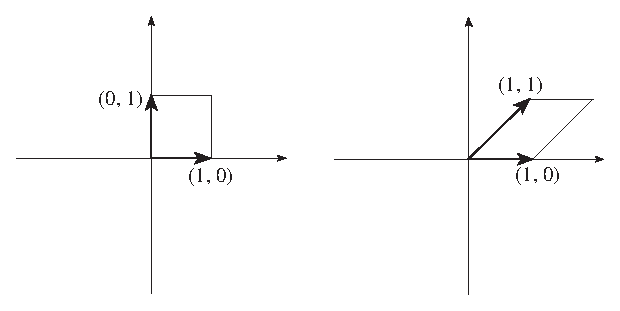
\includegraphics[width=2in]{SL2}
}
\end{center}
\caption{$SL_2({\Bbb R})$ acting on the unit square}
\label{SL2}
\end{figure}
 
 
 
\subsection*{The Orthogonal Group $O(n)$}
 
 
 
Another subgroup of $GL_n({\Bbb R})$ is the orthogonal group. A matrix
$A$ is {\bfi
orthogonal\/}\index{Orthogonal matrix}\index{Matrix!orthogonal} if
$A^{-1} = A^{\rm t}$. The {\bfi orthogonal
group\/}\index{Group!orthogonal}\index{Orthogonal group} consists of
the set of all orthogonal matrices. We write
$O(n)$\label{noteorthogonal} for the $n \times n$ orthogonal group. We
leave as an exercise the proof that $O(n)$ is a subgroup of $GL_n(
{\Bbb R})$.
 
 
\begin{example}{orthogonal}
The following matrices are orthogonal:
\[
\left(
\begin{array}{cc}
3/5 & -4/5 \\
4/5 & 3/5
\end{array}
\right), \; \;
\left(
\begin{array}{cc}
1/2 & -\sqrt{3}/2 \\
\sqrt{3}/2 & 1/2
\end{array}
\right), \; \;
\left(
\begin{array}{ccc}
-1/\sqrt{2} & 0 & 1/ \sqrt{2} \\
1/\sqrt{6} & -2/\sqrt{6} & 1/\sqrt{6} \\
1/ \sqrt{3} & 1/ \sqrt{3} & 1/ \sqrt{3} 
\end{array}
\right).
\]
\end{example}

 
There is a more geometric way of viewing the group $O(n)$. The
orthogonal matrices are exactly those matrices that preserve the
length of vectors. We can define the length of a vector using the
{\bfi Euclidean inner product},\index{Euclidean inner product} or
{\bfi dot product}, of two vectors. The Euclidean inner product of
two vectors ${\bold x}=(x_1, \ldots, x_n)^{\rm t}$ and ${\bold
y}=(y_1, \ldots, y_n)^{\rm t}$ is
\[
\langle  {\bold x}, {\bold y} \rangle
=
{\bold x}^{\rm t}  {\bold y}
=
(x_1, x_2, \ldots, x_n)
\left(
\begin{array}{c}
y_1 \\
y_2 \\
\vdots \\
y_n
\end{array}
\right)
=
x_1 y_1 + \cdots + x_n y_n.
\]
We define the length of a vector ${\bold x}=(x_1, \ldots, x_n)^{\rm
t}$ to be 
\[
\| {\bold x} \|\label{notelengthvect} 
= \sqrt{\langle  {\bold x}, {\bold x} \rangle} 
= \sqrt{x_1^2 + \cdots + x_n^2}.
\]
Associated with the notion of the length of a vector is the idea of
the distance between two vectors. We define the {\bfi distance\/}
between two vectors ${\bold x}$ and ${\bold y}$ to be $\| {\bold
x}-{\bold y} \|$. We leave as an exercise the proof of the following
proposition about the properties of Euclidean inner products.  
 
 
\begin{proposition}
Let ${\bold x}$, ${\bold y}$, and ${\bold w}$ be vectors in ${\Bbb
R}^n$ and $\alpha \in {\Bbb R}$. Then 
\begin{enumerate}
 
\rm \item \it
$\langle {\bold x}, {\bold y} \rangle = \langle {\bold y}, {\bold x}
\rangle$. 
 
\rm \item \it
$\langle {\bold x}, {\bold y} + {\bold w} \rangle = \langle {\bold x},
{\bold y} \rangle + \langle {\bold x}, {\bold w} \rangle$.
 
\rm \item \it
$\langle \alpha {\bold x}, {\bold y} \rangle = \langle {\bold x},
\alpha {\bold y} \rangle = \alpha \langle  {\bold x}, {\bold y}
\rangle$. 
 
\rm \item \it
$\langle {\bold x}, {\bold x} \rangle \geq 0$ with equality exactly
when ${\bold x} = 0$. 
 
\rm \item \it
If $\langle {\bold x}, {\bold y} \rangle = 0$  for all ${\bold x}$ in
${\Bbb R}^n$, then ${\bold y} = 0$. 
 
\end{enumerate}
\end{proposition}
 
 
\begin{example}{}
The vector ${\bold x} =(3,4)^{\rm t}$ has length $\sqrt{3^2 + 4^2} = 5$.  We
can also see that the orthogonal matrix 
\[
A=
\left(
\begin{array}{cc}
3/5 & -4/5 \\
4/5 & 3/5
\end{array}
\right)
\]
preserves the length of this vector. The vector $A{\bold x} =
(-7/5,24/5)^{\rm t}$ also has length 5. 
\end{example}
 
 
Since $\det(A A^{\rm t}) = \det(I) = 1$ and $\det(A) = \det( A^{\rm t}
)$, the determinant of any orthogonal matrix is either 1 or $-1$.
Consider the column vectors 
\[
{\bold a}_j
=
\left(
\begin{array}{c}
a_{1j} \\
a_{2j} \\
\vdots \\
a_{nj}
\end{array}
\right)
\]
of the orthogonal matrix
$A= (a_{ij})$. Since
$AA^{\rm t} = I$,
$\langle {\bold a}_r, {\bold a}_s \rangle = \delta_{rs}$,
where
\[
\delta_{rs}
=
\left\{
\begin{array}{cc}
1 & r = s \\
0 & r \neq s
\end{array}
\right.
\]
is the Kronecker delta\index{Kronecker delta}. Accordingly, column
vectors of an orthogonal matrix all have length 1; and the Euclidean
inner product of distinct column vectors is zero. Any set of vectors
satisfying these properties is called an {\bfi orthonormal
set}\index{Orthonormal set}. Conversely, given an $n \times n$ matrix
$A$ whose columns form an orthonormal set, $A^{-1} = A^{\rm t}$.
 
 
We say that a matrix $A$ is {\bfi
distance-preserving}\index{Matrix!distance-preserving}, {\bfi
length-preserving}\index{Matrix!length-preserving}, or {\bfi inner
product-preserving\/}\index{Matrix!inner product-preserving} when $\|
T{\bold x}- T{\bold y} \| =\| {\bold x}- {\bold y} \|$, $\| T{\bold x}
\| =\| {\bold x} \|$, or $\langle  T{\bold x}, T{\bold y} \rangle =
\langle {\bold x},{\bold y} \rangle$, respectively. The following
theorem, which characterizes the orthogonal group, says that these
notions are the same.
 
 
\begin{theorem}
Let $A$ be an $n \times n$ matrix.  The following statements are
equivalent. 
\begin{enumerate}
 
\rm \item \it
The columns of the matrix $A$ form an orthonormal set.
 
\rm \item \it
$A^{-1} = A^{\rm t}$.
 
\rm \item \it
For vectors ${\bold x}$ and ${\bold y}$, $\langle  A{\bold x}, A
{\bold y} \rangle = \langle  {\bold x}, {\bold y} \rangle$.
 
\rm \item \it
For vectors ${\bold x}$ and ${\bold y}$, $\| A{\bold x}- A{\bold y} \|
=\| {\bold x}- {\bold y} \|$. 
 
\rm \item \it
For any vector ${\bold x}$, $\| A{\bold x} \| = \| {\bold x}\|$.
 
\end{enumerate}
\end{theorem}
 
 
\begin{proof}
We have already shown (1) and (2) to be equivalent.
 
$(2) \Rightarrow (3)$.
\begin{eqnarray*}
\langle A{\bold x}, A{\bold y} \rangle
& = &
(A {\bold x})^{\rm t} A {\bold y} \\
& = &
{\bold x}^{\rm t} A^{\rm t} A {\bold y} \\
& = &
{\bold x}^{\rm t} {\bold y} \\
& = &
\langle {\bold x}, {\bold y} \rangle.
\end{eqnarray*}
 
$(3) \Rightarrow (2)$.
Since
\begin{eqnarray*}
\langle {\bold x}, {\bold x} \rangle
& = &
\langle A{\bold x}, A{\bold x} \rangle \\
& = &
{\bold x}^{\rm t} A^{\rm t} A {\bold y} \\
& = &
\langle {\bold x}, A^{\rm t} A{\bold x} \rangle,
\end{eqnarray*}
we know that $\langle {\bold x}, (A^{\rm t} A - I){\bold x} \rangle =
0$ for all ${\bold x}$.  Therefore, $A^{\rm t} A -I = 0$ or $A^{-1} =
A^{\rm t}$. 
 
 
$(3) \Rightarrow (4)$.
If $A$ is inner product-preserving, then $A$ is distance-preserving,
since 
\begin{eqnarray*}
\| A{\bold x} - A{\bold y} \|^2
& = &
\| A({\bold x} - {\bold y}) \|^2 \\
& = &
\langle
A({\bold x} - {\bold y}), A({\bold x} - {\bold y})
\rangle \\
& = &
\langle
{\bold x} - {\bold y}, {\bold x} - {\bold y}
\rangle \\
& = &
\| {\bold x} - {\bold y} \|^2.
\end{eqnarray*}
 
 
$(4) \Rightarrow (5)$.
If $A$ is distance-preserving, then $A$ is length-preserving. Letting
${\bold y} = 0$, we have
\[
\| A{\bold x}\|
= \| A{\bold x}- A{\bold y} \|
= \| {\bold x}- {\bold y} \|
= \| {\bold x} \|.
\]
 
 
$(5) \Rightarrow (3)$.
We use the following identity to show that length-preserving implies
inner product-preserving: 
\[
\langle {\bold x}, {\bold y} \rangle
=
\frac{1}{2}
\left[
\|{\bold x} +{\bold y}\|^2 -
 \|{\bold x}\|^2 - \|{\bold y}\|^2
\right].
\]
Observe that
\begin{eqnarray*}
\langle A {\bold x}, A {\bold y} \rangle
& = &
\frac{1}{2}
\left[
\|A {\bold x} + A {\bold y} \|^2
- \|A {\bold x} \|^2 -  \|A {\bold y} \|^2
\right] \\
& = &
\frac{1}{2}
\left[
\|A ( {\bold x} + {\bold y} ) \|^2
- \|A {\bold x} \|^2 -  \|A {\bold y} \|^2
\right] \\
& = &
\frac{1}{2}
\left[
\|{\bold x} + {\bold y}\|^2
- \|{\bold x}\|^2 - \|{\bold y}\|^2
\right] \\
& = &
\langle {\bold x}, {\bold y} \rangle.
\end{eqnarray*}
\end{proof}
 

 
 
\begin{figure}[htb]
\begin{center}
\centerline {
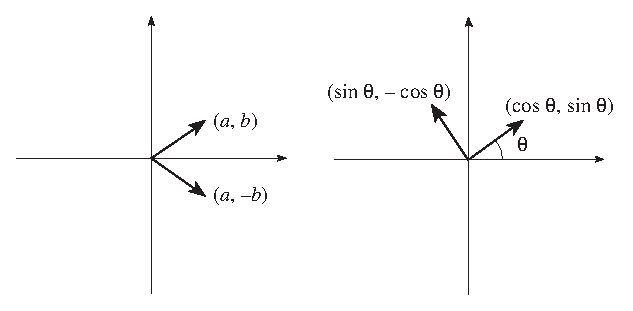
\includegraphics[width=2in]{O2}
}
\end{center}
\caption{$O(2)$ acting on ${\Bbb R}^2$}
\label{O2}
\end{figure}
 
\begin{example}{O2}
Let us examine the orthogonal group  on ${\Bbb R}^2$ a bit more
closely.  An element $T \in O(2)$ is determined by its action on
${\bold e}_1 = (1, 0)^{\rm t}$ and ${\bold e}_2 = (0, 1)^{\rm t}$. If
$T({\bold e}_1) = (a,b)^{\rm t}$, then $a^2 + b^2 = 1$ and $T({\bold
e}_2) = (-b, a)^{\rm t}$. Hence, $T$ can be represented by 
\[
A
=
\left(
\begin{array}{cc}
a & -b \\
b & a
\end{array}
\right)
=
\left(
\begin{array}{cc}
\cos \theta & - \sin \theta \\
\sin \theta & \cos \theta
\end{array}
\right),
\]
where $0 \leq \theta < 2 \pi$. A matrix $T$ in $O(2)$ either reflects
or rotates a vector in ${\Bbb R}^2$ (Figure~\ref{O2}). A reflection is
given by the matrix 
\[
\left(
\begin{array}{cc}
1 & 0 \\
0 & -1
\end{array}
\right),
\]
whereas a rotation by an angle $\theta$ in a counterclockwise direction
must come from a matrix of the form 
\[
\left(
\begin{array}{cc}
\cos \theta & \sin \theta \\
\sin \theta & -\cos \theta
\end{array}
\right).
\]
If $\det A =-1$, then $A$ gives a reflection.
\end{example}
 
 
 
Two of the other matrix or matrix-related groups that we will consider
are the special orthogonal group  and the group of Euclidean motions.
The {\bfi special orthogonal group}\index{Group!special orthogonal},
$SO(n)$\label{notespecialorthog}, is just the intersection of $O(n)$
and $SL_n({\Bbb R})$; that is, those elements in $O(n)$ with determinant
one. The {\bfi Euclidean
group}\index{Euclidean group}\index{Group!Euclidean},
$E(n)$\label{noteeuclidgroup}, can be written as ordered pairs $(A,
{\bold x})$, where $A$ is in $O(n)$ and ${\bold x}$ is in ${\Bbb
R}^n$. We define multiplication by
\[
(A, {\bold x}) (B, {\bold y})
=
(AB, A {\bold y} +{\bold x}).
\]
The identity of the group is $(I,{\bold 0})$; the inverse of $(A,
{\bold x})$ is $(A^{-1}, -A^{-1} {\bold x})$. In Exercise~6, you 
are asked to check that $E(n)$ is indeed a group under this operation.
 
 
 
 
\begin{figure}[hbt]
\begin{center}
\centerline {
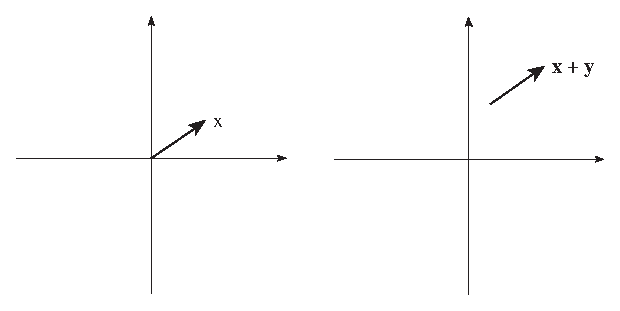
\includegraphics[width=2in]{Isometries}
}
\end{center}
\caption{Translations in ${\Bbb R}^2$}
\label{Isometries}
\end{figure}
 
 
 
 
 
\section{Symmetry}
 
 
 
 
An {\bfi isometry\/}\index{Isometry} or {\bfi rigid
motion\/}\index{Rigid motion} in ${\Bbb R}^n$  is a
distance-preserving function $f$ from ${\Bbb R}^n$ to ${\Bbb R}^n$.
This means that $f$ must satisfy 
\[
\| f({\bold x}) - f({\bold y}) \| =
\|{\bold x} - {\bold y} \|
\]
for all ${\bold x}, {\bold y} \in {\Bbb R}^n$. It is not difficult to
show that $f$ must be a one-to-one map. By Theorem~10.2, any element in
$O(n)$ is an isometry on ${\Bbb R}^n$; however, $O(n)$ does not
include all possible isometries on ${\Bbb R}^n$. Translation by a
vector ${\bold x}$, $T_{\bold y}({\bold x}) = {\bold x} + {\bold y}$
is also an isometry (Figure~\ref{Isometries}); however, $T$ cannot be
in $O(n)$ since it is not a linear map. 
 
 
 
We are mostly interested in isometries in ${\Bbb R}^2$. In fact, the
only isometries in ${\Bbb R}^2$ are rotations and reflections  about
the origin, translations, and combinations of the two. For example, a
{\bfi glide reflection\/}\index{Glide reflection} is a translation
followed by a reflection (Figure~\ref{Glide}).   In ${\Bbb R}^n$ all
isometries are given in the same manner. The proof is very easy to
generalize. 
 
 
\begin{figure}[htb]
\begin{center}
\centerline {
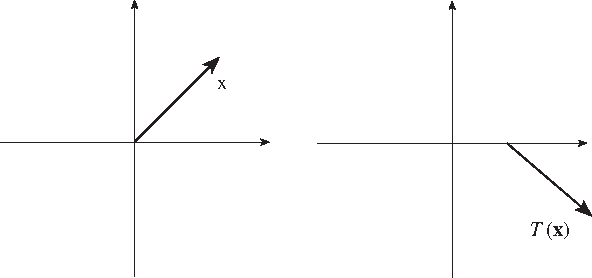
\includegraphics[width=2in]{Glide}
}
\end{center}
\caption{Glide reflections}
\label{Glide}
\end{figure}
 
 
\begin{lemma}
An isometry $f$ that fixes the origin in ${\Bbb R}^2$ is a linear
transformation.  In particular, $f$ is given by an element in $O(2)$. 
\end{lemma}
 
 
\begin{proof}
Let $f$ be an isometry in ${\Bbb R}^2$ fixing the origin. We will
first show that $f$ preserves inner products. Since $f(0) = 0$, $\|
f({\bold x})\| = \| {\bold x} \|$; therefore,
\begin{eqnarray*}
\| {\bold x} \|^2 - 2 \langle f({\bold x}), f({\bold y}) \rangle + \|
{\bold y} \|^2 
& = &
\| f({\bold x}) \|^2 - 2 \langle f({\bold x}), f({\bold y}) \rangle +
\| f({\bold y}) \|^2 \\ 
& = &
\langle
f({\bold x}) -  f({\bold y}), f({\bold x}) -  f({\bold y})
\rangle \\
& = &
\| f({\bold x}) -  f({\bold y}) \|^2 \\
& = &
\| {\bold x} -  {\bold y} \|^2 \\
& = &
\langle
{\bold x} -  {\bold y}, {\bold x} -  {\bold y} \rangle \\
& = &
\| {\bold x} \|^2 - 2 \langle {\bold x}, {\bold y} \rangle + \| {\bold
y} \|^2. 
\end{eqnarray*}
Consequently,
\[
\langle f({\bold x}), f({\bold y}) \rangle
=
\langle {\bold x}, {\bold y} \rangle.
\]
Now let ${\bold e}_1$ and ${\bold e_2}$ be $(1, 0)^{\rm t}$ and $(0,
1)^{\rm t}$, respectively. If 
\[
{\bold x} = (x_1, x_2) = x_1 {\bold e}_1 + x_2 {\bold e}_2,
\]
then
\[
f({\bold x})
=
\langle
f({\bold x}), f({\bold e}_1)
\rangle
f({\bold e}_1)
+\langle
f({\bold x}), f({\bold e}_2)
\rangle
f({\bold e}_2)
=
x_1 f({\bold e}_1)+x_2 f({\bold e}_2).
\]
The linearity of $f$ easily follows.
\end{proof}
 
 
\medskip
 
 
For any arbitrary isometry, $f$,  $T_{\bold x} f$ will fix the origin
for some vector ${\bold x}$ in ${\Bbb R}^2$; hence, $T_{\bold x}
f({\bold y}) = A {\bold y}$ for some matrix $A \in O(2)$.
Consequently, $f({\bold y}) = A {\bold y} + {\bold x}$.  Given the
isometries 
\begin{eqnarray*}
f({\bold y}) & = & A {\bold y} + {\bold x}_1 \\
g({\bold y}) & = & B {\bold y} + {\bold x}_2,
\end{eqnarray*}
their composition is
\[
f(g({\bold y})) =
f(B {\bold y} + {\bold x}_2) =
AB {\bold y} + A{\bold x}_2 + {\bold x}_1.
\]
This last computation allows us to identify the group of isometries on
${\Bbb R}^2$ with~$E(2)$. 
 
 
\begin{theorem}
The group of isometries on ${\Bbb R}^2$ is the Euclidean group,
$E(2)$. 
\end{theorem}
 
 
A {\bfi symmetry group\/}\index{Group!symmetry} in ${\Bbb R}^n$ is a
subgroup of the group of isometries on ${\Bbb R}^n$ that fixes a set
of points $X \subset {\Bbb R}^2$.  It is important to realize that the
symmetry group of $X$ depends {\em both\/} on ${\Bbb R}^n$ and on
$X$. For example, the symmetry group of the origin in ${\Bbb R}^1$ is
${\Bbb Z}_2$, but the symmetry group of the origin in ${\Bbb R}^2$ is
$O(2)$. 
 
 
\begin{theorem}
The only finite symmetry groups in ${\Bbb R}^2$ are ${\Bbb Z}_n$ and
$D_n$. 
\end{theorem}
 
 
\begin{proof}
Any finite symmetry group $G$ in ${\Bbb R}^2$ must be a finite
subgroup of $O(2)$; otherwise, $G$ would have an element in $E(2)$ of
the form $(A, {\bold x})$, where ${\bold x} \neq 0$.  Such an element
must have infinite order. 
 
 
By Example~6, elements in $O(2)$ are either rotations of the form
\[
R_{\theta}
=
\left(
\begin{array}{cc}
\cos \theta & - \sin \theta \\
\sin \theta & \cos \theta
\end{array}
\right)
\]
or reflections of the form
\[T_{\theta}
=
\left(
\begin{array}{cc}
\cos \theta & - \sin \theta \\
\sin \theta & \cos \theta
\end{array}
\right).
\]
Notice that $\det(R_{\theta})=1$,  $\det(T_{\theta})=-1$,
and $T_{\theta}^2=I$. We can divide the proof up into two cases.  In
the first case, all of the elements in $G$ have determinant one. In the
second case, there exists at least one element in $G$ with 
determinant~$-1$.  
 
 
{\em Case 1.}  
The determinant of every element in $G$ is one. In this case every
element in $G$ must be a rotation. Since $G$ is finite, there is a
smallest angle, say $\theta_0$, such that the corresponding element
$R_{\theta_0}$ is the smallest rotation in the positive direction.  We
claim that $R_{\theta_0}$ generates $G$.  If not, then for some
positive integer $n$ there is an angle $\theta_1$ between $n \theta_0$
and $(n+1) \theta_0$. If so, then $(n+1) \theta_0 - \theta_1$
corresponds to a rotation smaller than $\theta_0$, which contradicts
the minimality of $\theta_0$.   
 
 
 
{\em Case 2.}  
The group $G$ contains a reflection $T_{\theta}$.  The kernel of the
homomorphism $\phi : G \rightarrow \{-1, 1\}$ given by $A \mapsto
\det(A)$ consists of elements whose determinant is 1.  Therefore, $|G/
\ker \phi|=2$.  We know that the kernel is cyclic by the first case
and is a subgroup of $G$ of, say, order $n$. Hence, $|G| = 2n$. The
elements of $G$ are
\[
R_{\theta}, \ldots, R_{\theta}^{n-1},  TR_{\theta}, \ldots,
TR_{\theta}^{n-1}.
\]
These elements satisfy the relation
\[
TR_{\theta}T = R_{\theta}^{-1}.
\]
Consequently, $G$ must be isomorphic to $D_n$ in this case.
\end{proof}
 
 
 
 
\begin{figure}[thb]
\begin{center}
\centerline {
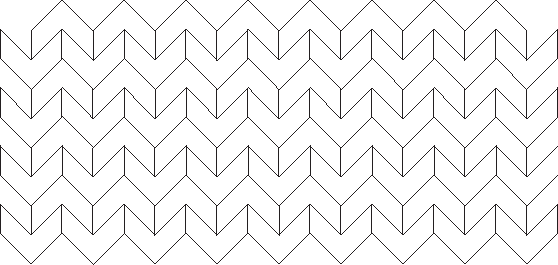
\includegraphics[width=2in]{Wallpaper}
}
\end{center}
\caption{A wallpaper pattern in ${\Bbb R}^2$}
\label{Wallpaper}
\end{figure}
 
 
 
\subsection*{The Wallpaper Groups}
 
 
 
Suppose that we wish to study wallpaper patterns in the plane or
crystals in three dimensions. Wallpaper patterns are simply repeating
patterns in the plane (Figure~\ref{Wallpaper}). The analogs of
wallpaper patterns in ${\Bbb R}^3$ are crystals, which we can think of
as repeating patterns of molecules in three dimensions
(Figure~\ref{Crystals}). The mathematical equivalent of a wallpaper or
crystal pattern is called a  lattice. 
 
 
 
\begin{figure}[hbt]
\begin{center}
\centerline {
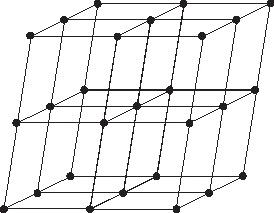
\includegraphics[width=2in]{Crystals}
}
\end{center}
\caption{A crystal structure in ${\Bbb R}^3$}
\label{Crystals}
\end{figure}
 
 

Let us examine wallpaper patterns in the plane a
little more closely. Suppose that ${\bold x}$ and ${\bold y}$ are
linearly independent vectors in ${\Bbb R}^2$; that is, one vector
cannot be a scalar multiple of the other. A {\bfi
lattice\/}\index{Lattice of points} of ${\bold x}$ and ${\bold y}$ is
the set of all linear combinations $m {\bold x} + n {\bold y}$, where
$m$ and $n$ are integers. The vectors ${\bold x}$ and ${\bold y}$ are
said to be a {\bfi basis\/}\index{Basis of a lattice} for the lattice.
 
 
\begin{figure}[htb]
\begin{center}
\centerline {
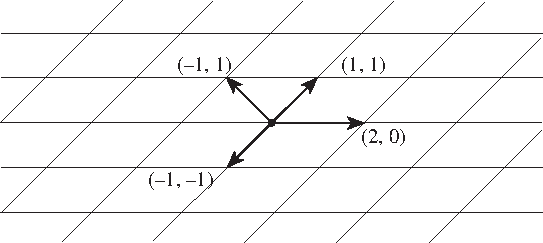
\includegraphics[width=2in]{LatticeExample}
}
\end{center}
\caption{A lattice in  ${\Bbb R}^2$}
\label{lattice}
\end{figure}
 
 
Notice that a lattice can have several bases. For example, the vectors
$(1,1)^{\rm t}$ and $(2,0)^{\rm t}$ have the  same lattice as the
vectors $(-1, 1)^{\rm t}$ and $(-1, -1)^{\rm t}$
(Figure~\ref{lattice}). However, any lattice is completely determined
by a basis. Given two bases for the same lattice, say $\{ {\bold x}_1,
{\bold x}_2 \}$ and $\{ {\bold y}_1, {\bold y}_2 \}$, we can write 
\begin{eqnarray*}
{\bold y}_1 & = & \alpha_1  {\bold x}_1 + \alpha_2 {\bold x}_2 \\
{\bold y}_2 & = & \beta_1  {\bold x}_1 + \beta_2 {\bold x}_2,
\end{eqnarray*}
where $\alpha_1$, $\alpha_2$, $\beta_1$, and $\beta_2$ are integers.
The matrix corresponding to this transformation is 
\[
U
=
\left(
\begin{array}{cc}
\alpha_1 & \alpha_2 \\
\beta_1 & \beta_2
\end {array}
\right).
\]
If we wish to give ${\bold x}_1$ and ${\bold x}_2$ in terms of ${\bold
y}_1$ and ${\bold y}_2$, we need only calculate $U^{-1}$; that is, 
\[
U^{-1}
\left(
\begin{array}{c}
{\bold y}_1 \\
{\bold y}_2
\end{array}
\right)
=
\left(
\begin{array}{c}
{\bold x}_1 \\
{\bold x}_2
\end{array}
\right).
\]
Since $U$ has integer entries, $U^{-1}$ must also have integer
entries; hence the determinants of both $U$ and $U^{-1}$ must be
integers. Because $U U^{-1} = I$,  
\[
\det(U U^{-1}) =\det(U) \det( U^{-1}) = 1;
\]
consequently, $\det(U) = \pm 1$. A matrix with determinant $\pm 1$ and
integer entries is called {\bfi unimodular}\index{Matrix!unimodular}.
For example, the matrix 
\[
\left(
\begin{array}{cc}
3 & 1 \\
5 & 2
\end{array}
\right)
\]
is unimodular. It should be clear that there is a minimum length for
vectors in a lattice.  
 
 
We can classify lattices by studying their symmetry groups. The
symmetry group of a lattice is the subgroup of $E(2)$ that maps the
lattice to itself. We consider two lattices in ${\Bbb R}^2$ to be
equivalent if they have the same symmetry group.  Similarly,
classification of crystals in ${\Bbb R}^3$ is accomplished by
associating a symmetry group, called a {\bfi space group}, with each
type of crystal\index{Group!space}. Two lattices are considered
different if their space groups are not the same.  The natural
question that now arises is how many space groups exist. 
 
 
A space group is composed of two parts: a {\bfi translation
subgroup\/}\index{Subgroup!translation} and a {\bfi point
group}\index{Group!point}.  The translation subgroup is an infinite
abelian subgroup of the space group made up of the translational
symmetries of the crystal; the point group is a finite group 
consisting  of rotations and reflections of the crystal about a point.
More specifically, a space group is a subgroup of $G \subset E(2)$
whose translations are a set of the form $\{ (I, t) : t \in L \}$,
where $L$ is a lattice. Space groups are, of course, infinite. Using
geometric arguments, we can prove the following theorem (see [5] or [6]).
 
 
 
 
\begin{theorem}
Every translation group in ${\Bbb R}^2$ is isomorphic to ${\Bbb Z}
\times {\Bbb Z}$.
\end{theorem}
 
 
\begin{figure}[bht]
\begin{center}
\centerline {
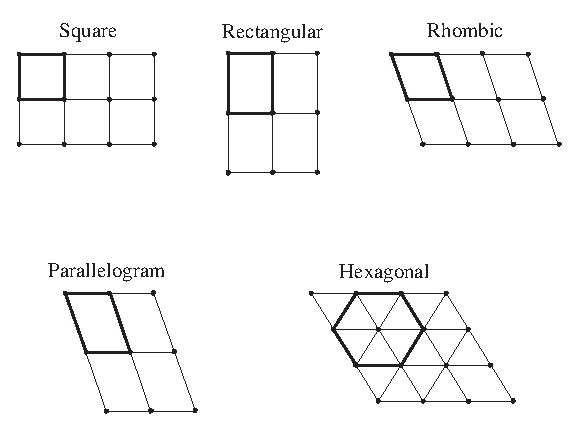
\includegraphics[width=2in]{TypeLattice}
}
\end{center}
\caption{Types of lattices in  ${\Bbb R}^2$}
\label{Types}
\end{figure}
 
 
The point group of $G$ is $G_0 = \{A : (A,b) \in G \mbox{ for some
$b$}  \}$. In particular, $G_0$ must be a subgroup of $O(2)$. Suppose
that ${\bold x}$ is a vector in a lattice $L$ with space group $G$,
translation group $H$, and point group $G_0$. For any element $(A,
{\bold y})$ in $G$,   
\begin{eqnarray*}
(A, {\bold y}) (I, {\bold x}) (A, {\bold y})^{-1}
& = &
(A,A {\bold x} + {\bold y}) (A^{-1},-A^{-1} {\bold y}) \\
& = &
(A A^{-1},-A A^{-1} {\bold y} + A {\bold x} + {\bold y}) \\
& = &
(I, A {\bold x});
\end{eqnarray*}
hence, $(I, A {\bold x})$ is in the translation group of $G$. More
specifically, $A {\bold x}$ must be in the lattice $L$. It is
important to note that $G_0$ is not usually a subgroup of the space
group $G$; however, if $T$ is the translation subgroup of $G$, then
$G/T \cong G_0$. The proof of the following theorem can be found in
[2], [5], or~[6].
 
 
 
\begin{theorem}
The point group in the wallpaper groups is isomorphic to ${\Bbb Z}_n$
or $D_n$, where $n = 1, 2, 3, 4, 6$. 
\end{theorem}
 
 
To answer the question of how the point groups and the translation
groups can be combined, we must look at the different types of
lattices. Lattices can be classified by the structure of a single
lattice cell. The possible cell shapes are parallelogram, rectangular,
square, rhombic, and hexagonal (Figure~\ref{Types}). The wallpaper
groups can now be classified according to the types of reflections
that occur in each group: these are ordinarily reflections, glide
reflections, both, or none.
 
 
 
\begin{table}[htb]
\caption{The 17 wallpaper groups}{\small
\begin{center}
\begin{tabular}{|l|l|l|l|}
\hline
Notation and &             &              & Reflections  \\
Space Groups & Point Group & Lattice Type & or Glide Reflections? \\
\hline
p1 & ${\Bbb Z}_1$ & parallelogram & none \\
p2 & ${\Bbb Z}_2$ & parallelogram & none \\
p3 & ${\Bbb Z}_3$ & hexagonal & none \\
p4 & ${\Bbb Z}_4$ & square & none \\
p6 & ${\Bbb Z}_6$ & hexagonal & none \\
pm & $D_1$ & rectangular & reflections \\
pg & $D_1$ & rectangular & glide reflections\\
cm & $D_1$ & rhombic & both \\
pmm & $D_2$ & rectangular & reflections \\
pmg & $D_2$ & rectangular & glide reflections \\
pgg & $D_2$ & rectangular & both \\
c2mm & $D_2$ & rhombic & both \\
p3m1, p31m & $D_3$ & hexagonal & both \\
p4m, p4g & $D_4$ & square & both \\
p6m & $D_6$ & hexagonal & both \\
\hline
\end{tabular}
\end{center}
}
\end{table}
 
 
\begin{theorem}
There are exactly 17 wallpaper groups.
\end{theorem}
 
 
\begin{figure}[htb]
\begin{center}
\centerline {
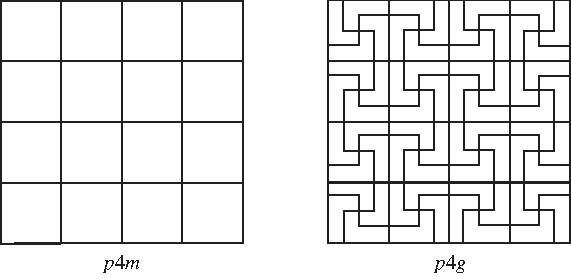
\includegraphics[width=2in]{p4m}
}
\end{center}
\caption{The wallpaper groups p4m and  p4g}
\label{p4m}
\end{figure}
 
 
 
The 17 wallpaper groups are listed in Table~10.1. The groups p3m1 and
p31m can be distinguished by whether or not all of their threefold
centers lie on the reflection axes: those of p3m1 must, whereas those
of p31m may not. Similarly, the fourfold centers of p4m must lie on
the reflection axes whereas those of p4g need not (Figure~\ref{p4m}).
The complete proof of this theorem can be found in several of the
references at the end of this chapter, including [5], [6], [10],
and~[11]. 
 
 
 
\histhead
 
 
\noindent{\small \histf
Symmetry groups have intrigued mathematicians for a long time.
Leonardo da Vinci was probably the first person to know all of the
point groups.  At the International Congress of Mathematicians in
1900, David Hilbert\index{Hilbert, David} gave a now-famous address
outlining 23 problems to guide mathematics in the twentieth
century.  Hilbert's eighteenth problem asked whether or not
crystallographic groups in $n$ dimensions were always finite.  In
1910, L.~Bieberbach\index{Bieberbach, L.} proved that crystallographic
groups are finite in every dimension.  Finding out how many of these
groups there are in each dimension is another matter. In ${\Bbb R}^3$
there are 230 different space groups; in ${\Bbb R}^4$ there are 4783.
No one has been able to compute the number of space groups for ${\Bbb
R}^5$ and beyond. It is interesting to note that the crystallographic
groups were found mathematically for ${\Bbb R}^3$ before the 230
different types of crystals were actually discovered in nature.
\histbox
}
 
 
 
\markright{EXERCISES}
\section*{Exercises}
\exrule
 
 
{\small
\begin{enumerate}
 
 
 
\bf\item\rm
Prove the identity
\[
\langle {\bold x}, {\bold y} \rangle = \frac{1}{2}
\left[
\|{\bold x} + {\bold y}\|^2 - \|{\bold x}\|^2 - \| {\bold y}\|^2
\right].
\]
 
 
\bf\item\rm
Show that $O(n)$ is a group.
 
 
\bf\item\rm
Prove that the following matrices are orthogonal. Are any of
these matrices in $SO(n)$?
 
\vspace{3pt}        %two column exercise list
 
\hspace{-7pt}
\begin{minipage}[t]{4.6in}
\noindent
\begin{minipage}[t]{2.25in}
\begin{itemize}
 
 \item[{\bf (a)}]
\raisebox{-5.5pt}{\parbox{1.85in}{
\[
\left(
\begin{array}{cc}
1/\sqrt{2} & -1/\sqrt{2} \\
1/\sqrt{2} & 1/\sqrt{2}
\end{array}
\right)
\]
}}

 
 \item[{\bf (c)}]
\raisebox{-11.5pt}{\parbox{1.85in}{
\[
\left(
\begin{array}{ccc}
4/ \sqrt{5} & 0 & 3 / \sqrt{5} \\
-3 / \sqrt{5} & 0 & 4 / \sqrt{5} \\
0 & -1 & 0
\end{array}
\right)
\] 
}}

\end{itemize}
\end{minipage} \hfill
\begin{minipage}[t]{2.25in}
\begin{itemize}
 
 \item[{\bf (b)}]
\raisebox{-5.5pt}{\parbox{1.85in}{
\[
\left(
\begin{array}{cc}
1 / \sqrt{5} & 2 / \sqrt{5} \\
- 2 /\sqrt{5} & 1/ \sqrt{5}
\end{array}
\right)
\]
}} 
 
 
 \item[{\bf (d)}]
\raisebox{-11.5pt}{\parbox{1.85in}{
\[
\left(
\begin{array}{ccc}
1/3 & 2/3 & - 2/3 \\
- 2/3 & 2/3 & 1/3 \\
-2/3 & 1/3 & 2/3
\end{array}
\right)
\]
}}
 
 
\end{itemize}
\end{minipage}
\end{minipage}
 
\vspace{2pt}        %end two column exercise list
 
 
 
\bf\item\rm %%%%%%%%%%%%%%%%%%%%%%
Determine the symmetry group of each of the figures in
Figure~\ref{Determine}. 
\begin{figure}[htb]
\begin{center}
\centerline {
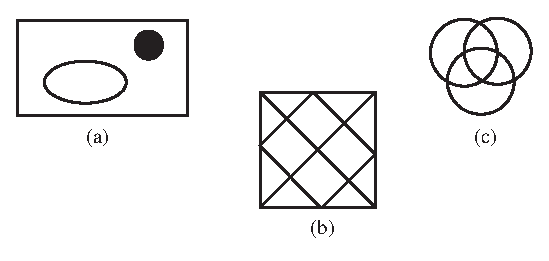
\includegraphics[width=2in]{SymmetryGrp}
}
\end{center}
\caption{}
\label{Determine}
\end{figure}
 
 
\bf\item\rm
Let ${\bold x}$, ${\bold y}$, and ${\bold w}$ be vectors in ${\Bbb
R}^n$ and $\alpha \in {\Bbb R}$.  Prove each of the following
properties of inner products.
\begin{enumerate}
 
 \bf\item\rm
$\langle {\bold x}, {\bold y} \rangle = \langle {\bold y}, {\bold x}
\rangle$. 
 
 \bf\item\rm
$\langle {\bold x}, {\bold y} + {\bold w} \rangle = \langle
{\bold x}, {\bold y} \rangle + \langle {\bold x}, {\bold w}
\rangle$.
 
 \bf\item\rm
$\langle \alpha {\bold x}, {\bold y} \rangle = \langle
{\bold x}, \alpha {\bold y} \rangle = \alpha \langle  {\bold
x}, {\bold y} \rangle$.
 
 \bf\item\rm
$\langle {\bold x}, {\bold x} \rangle \geq 0$ with equality exactly
when ${\bold x} = 0$. 
 
 \bf\item\rm
If $\langle {\bold x}, {\bold y} \rangle = 0$  for all ${\bold x}$ in
${\Bbb R}^n$, then ${\bold y} = 0$. 
 
\end{enumerate}
 
 
\bf\item\rm
Verify that
\[
E(n)
=
\{(A, {\bold x}) : A \in O(n) \mbox{ and } {\bold x} \in
{\Bbb R}^n \}
\]
is a group.
 
 
\bf\item\rm
Prove that $\{ (2,1), (1,1) \}$  and $\{ ( 12, 5), ( 7, 3) \}$ are bases
for the same lattice. 
 
 
\bf\item\rm
Let $G$ be a subgroup of $E(2)$ and suppose that $T$ is the
translation subgroup of $G$.  Prove that the point group of $G$ is
isomorphic to $G/T$. 
 
 
\bf\item\rm
Let $A \in SL_2({\Bbb R})$ and suppose that the vectors ${\bold x}$
and ${\bold y}$ form two sides of a parallelogram in ${\Bbb R}^2$.
Prove that the area of this parallelogram is the same as the area of
the parallelogram with sides $A{\bold x}$ and $A{\bold y}$. 
 
 
\bf\item\rm
Prove that $SO(n)$ is a normal subgroup of $O(n)$.
 
 
\bf\item\rm
Show that any isometry $f$ in ${\Bbb R}^n$ is a one-to-one map.
 
 
\bf\item\rm
Show that an element in $E(2)$ of the form $(A, {\bold x})$,
where ${\bold x} \neq 0$, has infinite order.
 
 
\bf\item\rm
Prove or disprove: There exists an infinite abelian subgroup of 
$O(n)$.
 
 
\bf\item\rm
Let ${\bold x} = (x_1, x_2)$ be a point on the unit circle in ${\Bbb
R}^2$; that is, $x_1^2 + x_2^2 = 1$. If $A \in O(2)$, show that $A
{\bold x}$ is also a point on the unit circle. 
 
 
 
\bf\item\rm
Let $G$ be a group with a subgroup $H$ (not necessarily normal) and a
normal subgroup $N$. Then $G$ is a {\bfi semidirect
product\/}\index{Semidirect product} of $N$ by $H$ if  
\begin{itemize}
 
 \item
$H \cap N = \{ id \}$;
 
 \item
$HN=G$.
 
\end{itemize}
Show that each of the following is true.
\begin{enumerate}
 
 \bf\item\rm
$S_3$ is the semidirect product of $A_3$ by $H = \{(1), (12) \}$.
 
 \bf\item\rm
The quaternion group, $Q_8$, cannot be written as a semidirect product. 
 
 \bf\item\rm
$E(2)$ is the semidirect product of $O(2)$ by $H$, where $H$ consists
of all translations in ${\Bbb R}^2$. 
 
\end{enumerate}
 
 
 
\bf\item\rm
Determine which of the 17 wallpaper groups preserves the symmetry of
the pattern in Figure~\ref{Wallpaper}.  
 
\begin{figure}[htb]
\begin{center}
\centerline {
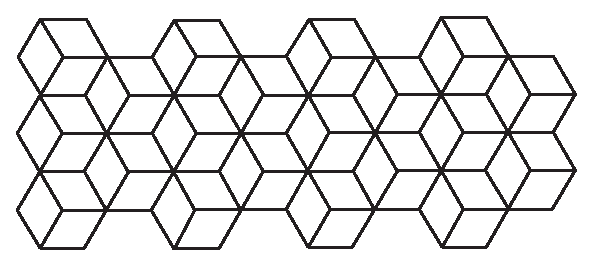
\includegraphics[width=2in]{p6m}
}
\end{center}
\caption{}
\label{For17}
\end{figure}
 
\bf\item\rm
Determine which of the 17 wallpaper groups preserves the symmetry of
the pattern in Figure~\ref{For17}.  
 
 
 
\bf\item\rm
Find the rotation group of a dodecahedron.
 
  
 
\bf\item\rm
For each of the 17 wallpaper groups, draw a wallpaper pattern having
that group as a symmetry group.  
 
\end{enumerate}
}
 
 
 
\subsection*{References and Suggested Readings}
 
 
 
{\small
\begin{itemize}
 
\item[{\bf [1]}]
Coxeter, H. M. and Moser, W. O. J. {\it Generators and
Relations for Discrete Groups}, 3rd ed. Springer-Verlag, New
York, 1972.
 
\item[{\bf [2]}]
Grove, L. C. and Benson, C. T. {\it Finite Reflection
Groups}. 2nd ed. Springer-Verlag, New York, 1985.
 
\item[{\bf [3]}]
Hiller, H. ``Crystallography and Cohomology of Groups,''
{\it American Mathematical Monthly} {\bf 93} (1986), 765--79.
 
\item[{\bf [4]}]
Lockwood, E. H. and Macmillan, R. H. {\it Geometric
Symmetry}. Cambridge University Press, Cambridge, 1978.
 
\item[{\bf [5]}]
Mackiw, G. {\it Applications of Abstract Algebra}. Wiley,
New York, 1985.
 
 
\item[{\bf [6]}]
Martin,  G.  {\it Transformation  Groups:  An Introduction to
Symmetry}.  Springer-Verlag, New York, 1982.
 
  
\item[{\bf [7]}]
Milnor, J. ``Hilbert's Problem 18: On Crystallographic
Groups, Fundamental Domains, and Sphere Packing,'' {\it
Proceedings of Symposia in Pure Mathematics} {\bf 18},
American Mathematical Society, 1976.
 
\item[{\bf [8]}]
Phillips, F. C. {\it An Introduction to Crystallography}.
4th ed. Wiley, New York, 1971.
 
\item[{\bf [9]}]
Rose, B. I. and Stafford, R. D. ``An Elementary Course in
Mathematical Symmetry,'' {\it American Mathematical Monthly} {\bf
88} (1980), 54--64.
 
 
\item[{\bf [10]}]
Schattschneider, D. ``The Plane Symmetry Groups: Their
Recognition and Their Notation,'' {\it American Mathematical 
Monthly} {\bf 85} (1978), 439--50.
 
 
\item[{\bf [11]}]
Schwarzenberger, R. L. ``The 17 Plane Symmetry Groups,'' {\it
Mathematical  Gazette} {\bf 58} (1974), 123--31. 
 
 
\item[{\bf [12]}]
Weyl, H. {\it Symmetry}. Princeton University Press, Princeton, NJ,
1952. 
 
 
\end{itemize}
}
 
 
 
 
   %Groups of Symmetries
%%%%(c)
%%%%(c)  This file is a portion of the source for the textbook
%%%%(c)
%%%%(c)    Abstract Algebra: Theory and Applications
%%%%(c)    Copyright 1997 by Thomas W. Judson
%%%%(c)
%%%%(c)  See the file COPYING.txt for copying conditions
%%%%(c)
%%%%(c)
\chap{The Structure of  Groups}{struct}
 

The ultimate goal of group theory is to classify all groups up to
isomorphism; that is, given a particular group, we should be able to
match it up with a known group via an isomorphism. For example, we
have already proved that any finite cyclic group of order $n$ is
isomorphic to ${\Bbb Z}_n$; hence, we ``know'' all finite cyclic
groups. It is probably not reasonable to expect that we will ever know
all groups; however, we can often classify certain types of groups or
distinguish between groups in special cases.  

In this chapter we will characterize all finite abelian groups. We
shall also investigate groups with sequences of subgroups.  If a group
has a sequence of subgroups, say 
\[
G = H_n \supset H_{n-1} \supset \cdots \supset H_1 \supset H_0 = \{ e
\}, 
\]
where each subgroup $H_i$ is normal in $H_{i+1}$ and each of the
factor groups $H_{i+1}/H_i$ is abelian, then $G$ is a solvable group.
In addition to allowing us to distinguish between certain classes of
groups, solvable groups turn out to be central to the study of
solutions to polynomial equations.
 

\section{Finite Abelian Groups}

In our investigation of cyclic groups we found that every group of
prime order was isomorphic to ${\Bbb Z}_p$, where $p$ was a prime
number.  We also determined that ${\Bbb Z}_{mn} \cong {\Bbb Z}_m
\times {\Bbb Z}_n$ when $\gcd(m, n) =1$. In fact, much more is true.
Every finite abelian group is isomorphic to a direct product of cyclic
groups of prime power order; that is, every finite abelian group is
isomorphic to a group of the type 
\[
{\Bbb Z}_{p_1^{\alpha_1}} \times \cdots \times {\Bbb
Z}_{p_n^{\alpha_n}}.
\]

First, let us examine a slight generalization  of finite abelian
groups. Suppose that $G$ is a group and let $\{ g_i\}$ be a set of 
elements in $G$, where $i$ is in some index set $I$ (not necessarily 
finite).  The smallest subgroup of $G$ containing all of the $g_i$'s 
is the subgroup of $G$ {\bfi generated\/} by the $g_i$'s. If this 
subgroup of $G$ is in fact all of $G$, then $G$ is generated by the 
set $\{g_i : i \in I \}$. In this case the $g_i$'s are said to be 
the {\bfi generators\/}\index{Generators for a 
group}\index{Group!generators of} of $G$. If there is a finite set 
$\{ g_i : i \in I \}$ that generates $G$, then $G$ is {\bfi finitely 
generated}\index{Group!finitely generated}\index{Finitely generated 
group}.
 
 
\begin{example}{finite_groups}
Obviously, all finite groups are finitely generated. For example, the
group $S_3$ is generated by the permutations $(12)$ and $(123)$. The
group ${\Bbb Z} \times {\Bbb Z}_n$ is an infinite group but is
finitely generated by $\{ (1,0), (0,1) \}$.
\end{example}
 
 
 
\begin{example}{infinite_groups}
Not all groups are finitely generated.  Consider the rational numbers
${\Bbb Q}$ under the operation of addition. Suppose that ${\Bbb Q}$ is
finitely generated with generators $p_1/q_1, \ldots, p_n/q_n$, where
each $p_i/q_i$ is a fraction expressed in its lowest terms.  Let $p$
be some prime that does not divide any of the denominators $q_1,
\ldots, q_n$. We claim that $1/p$ cannot be in the subgroup of ${\Bbb
Q}$ that is generated by  $p_1/q_1, \ldots, p_n/q_n$, since $p$ does
not divide the denominator of any element in this subgroup. This fact
is easy to see since the sum of any two generators is
\[
p_i / q_i + p_j / q_j = (p_i q_j + p_j q_i)/(q_i q_j).
\]
\end{example}
 
 
\begin{theorem}
Let $H$ be the subgroup of a group $G$ that is generated by $\{ g_i
\in G : i \in I \}$. Then $h \in H$ exactly when it is a product of
the form 
\[
h = g_{i_1}^{\alpha_1} \cdots g_{i_n}^{\alpha_n},
\]
where the $g_{i_k}$'s are not necessarily distinct.
\end{theorem}
 
 
The reason that powers of a fixed $g_i$ may occur several times in the
product is that we may have a nonabelian group. However, if the group
is abelian, then the $g_i$'s need occur only once. For example, a
product such as $a^{-3} b^5 a^7$ could always be simplified (in this
case, to $a^4 b^5$). 
 
 
\medskip
 
 
\begin{proof}
Let $K$ be the set of all products of the form $g_{i_1}^{\alpha_1}
\cdots g_{i_n}^{\alpha_n}$, where the $g_{i_k}$'s are not necessarily
distinct. Certainly $K$ is a subset of $H$.  We need only show that
$K$ is a subgroup of $G$. If this is the case, then $K=H$, since $H$ is
the smallest subgroup containing all the $g_i$'s.
 
 
Clearly, the set $K$ is closed under the group operation. Since $g_i^0
=1$, the identity is in $K$. It remains to show that the inverse of an
element  $g =g_1^{k_1} \cdots g_{i_n}^{k_n}$ in $K$ must also be in
$K$. However, 
\[
g^{-1}
= (g_1^{k_1} \cdots g_{i_n}^{k_n})^{-1}
= (g_1^{-k_n} \cdots g_{i_n}^{-k_1}).
\]
\end{proof}
 
\medskip
 
Now let us restrict our attention to finite abelian groups. We can
express any finite abelian group as a finite direct product of cyclic
groups. More specifically, letting $p$ be prime, we define a group $G$
to be a {\bfi $p$-group\/}\index{Group!$p$-group} if every element in 
$G$ has as its order a power of $p$. For example, both ${\Bbb Z}_2 
\times {\Bbb Z}_2$ and ${\Bbb Z}_4$ are $2$-groups, whereas 
${\Bbb Z}_{27}$ is a $3$-group. We shall prove that every finite 
abelian group is isomorphic to a direct product of cyclic $p$-groups. 
Before we  state the main theorem concerning finite abelian groups, we 
shall consider a special case.
 
 
\begin{theorem}
Every finite abelian group $G$ is the direct product of $p$-groups. 
\end{theorem}
 
 
\begin{proof}
If $|G|= 1$, then the theorem is trivial.  Suppose that the order of
$G$ is greater than 1, say 
\[
|G| = p_1^{\alpha_1} \cdots p_n^{\alpha_n},
\]
where $p_1, \ldots, p_n$ are all prime, and define $G_i$ to be the set
of elements in $G$ of order $p_i^k$ for some integer $k$. Since $G$ is
an abelian group, we are guaranteed that $G_i$ is a subgroup of $G$
for $i = 1, \ldots, n$. We must show that
\[
G = G_1 \times \cdots \times G_n.
\]
That is, we must be able to write every $g \in G$ as a unique product
$g_{p_1} \cdots g_{p_n}$ where $g_{p_i}$ is of the order of some power
of $p_i$. Since the order of $g$ divides the order of $G$, we know
that 
\[
|g| = p_1^{\beta_1}  p_2^{\beta_2} \cdots p_n^{\beta_n}
\]
for integers $\beta_1, \ldots, \beta_n$. Letting $a_i = |g| /
p_i^{\beta_i}$, the $a_i$'s are relatively prime; hence, there exist
integers $b_1, \ldots, b_n$ such that $a_1 b_1 + \cdots + a_n b_n =
1$. Consequently, 
\[
g = g^{a_1 b_1 + \cdots + a_n b_n} = g^{a_1 b_1} \cdots  g^{a_n b_n}. 
\]
Since
\[
g^{(a_i b_i ) p_i^{\beta_i}} = g^{b_i |g|} = e,
\]
it follows that $g^{a_i b_i}$ must be in $G_{i}$. Let $g_i =
g^{a_i b_i}$. Then $g = g_1 \cdots g_n$ and $G_i \cap G_j = \{ e \}$ for $i
\neq j$. 
 
 
To show uniqueness, suppose that $g = g_1 \cdots g_n = h_1 \cdots h_n$,
with $h_i \in G_i$. Then
\[
e = (g_1 \cdots g_n)(h_1 \cdots h_n)^{-1} = g_1 h_1^{-1} \cdots g_n
h_n^{-1}. 
\]
The order of $g_i h_i^{-1}$ is a power of $p_i$; hence, the order of
$g_1 h_1^{-1} \cdots g_n h_n^{-1}$ is the least common multiple of the
orders of the $g_i h_i^{-1}$.  This must be 1, since the order of the
identity is 1. Therefore, $|g_i h_i^{-1}| =1$ or $g_i =h_i$ for $i =
1, \ldots, n$.
\mbox{\hspace{1in}}
\end{proof}
 
 
\medskip

We shall now state the Fundamental Theorem of Finite Abelian Groups. 
 
 
\begin{theorem}
{\bf (Fundamental Theorem of Finite Abelian
Groups)}\index{Fundamental Theorem!of Finite Abelian Groups} 
Every finite abelian group $G$ is isomorphic to a direct product of
cyclic groups of the form 
\[
{\Bbb Z}_{p_1^{ \alpha_1 }}
\times
{\Bbb Z}_{p_2^{ \alpha_2 }}
\times
\cdots
\times
{\Bbb Z}_{p_n^{ \alpha_n }}
\]
where the $p_i$'s are primes (not necessarily distinct).
\end{theorem}
 
 
\begin{example}{abelian540}
Suppose that we wish to classify all abelian groups of order $540=2^2
\cdot 3^3 \cdot 5$.  The Fundamental Theorem of Finite Abelian Groups 
tells us that we have the following six possibilities.
\begin{itemize}
 
\item
${\Bbb Z}_2 \times {\Bbb Z}_2 \times {\Bbb Z}_3
\times {\Bbb Z}_3 \times {\Bbb Z}_3 \times {\Bbb Z}_5$;
 
\item
${\Bbb Z}_2 \times {\Bbb Z}_2 \times {\Bbb Z}_3
\times {\Bbb Z}_9 \times {\Bbb Z}_5$;
 
 
\item
${\Bbb Z}_2 \times {\Bbb Z}_2
\times {\Bbb Z}_{27} \times {\Bbb Z}_5$;
 
 
\item
${\Bbb Z}_4 \times {\Bbb Z}_3
\times {\Bbb Z}_3 \times {\Bbb Z}_3 \times {\Bbb Z}_5$;
 
\item
${\Bbb Z}_4 \times {\Bbb Z}_3
\times {\Bbb Z}_9 \times {\Bbb Z}_5$;
 
\item
${\Bbb Z}_4 \times {\Bbb Z}_{27} \times {\Bbb Z}_5$.
 
\end{itemize}
\end{example}
 
The  proof of the Fundamental Theorem relies on the following lemma.

\begin{lemma}\label{struct:lemma:finite_abelian}
Let $G$ be a finite abelian $p$-group and suppose that $g \in G$ has
maximal order. Then $G$ can be written as $\langle g \rangle \times H$
for some subgroup $H$~of~$G$. 
\end{lemma}
 
 
\begin{proof}
Suppose that the order of $G$ is $p^n$.  We shall induct on $n$. If
$n= 1$, then $G$ is cyclic of order $p$ and must be generated by $g$.
Suppose now that the statement of the lemma holds for all integers $k$
with $1 \leq k < n$ and let $g$ be of maximal order in $G$, say
$|g| = p^{m}$.  Then $a^{p^m} = e$ for all $a \in G$. Now choose $h$
in $G$ such that $h \notin \langle g \rangle$, where $h$ has the
smallest possible order.  Certainly such an $h$ exists; otherwise, $G
= \langle g \rangle$ and we are done.  Let $H = \langle h \rangle$.
 
 
We claim that $\langle g \rangle \cap H = \{ e \}$. It suffices to
show that $|H|=p$.  Since $|h^p| = |h| / p$, the order of $h^p$ is
smaller than the order of $h$ and must be in $\langle g \rangle$ by
the minimality of $h$; that is, $h^p = g^r$ for some number $r$.
Hence, 
\[
(g^r)^{p^{m-1}} = (h^p)^{p^{m-1}} = h^{p^{m}} = e,
\]
and the order of $g^r$ must be less than or equal to $p^{m-1}$.
Therefore, $g^r$ cannot generate $\langle g \rangle$.  Notice that $p$
must occur as a factor of $r$, say $r = ps$, and $h^p = g^r = g^{ps}$.
Define $a$ to be $g^{-s}h$. Then $a$ cannot be in $\langle g \rangle$;
otherwise, $h$ would also have to be in $\langle g \rangle$. Also, 
\[
a^p = g^{-sp} h^p = g^{-r} h^p = h^{-p} h^p = e.
\]
We have now formed an element $a$ with order $p$ such that $a \notin
\langle g \rangle$. Since $h$ was chosen to have the smallest order of
all of the elements that are not in $\langle g \rangle$, $|H|  = p$.
 
 
Now we will show that the order of $gH$ in the factor group $G/H$ 
must be the same as the order of $g$ in $G$.  If $|gH| < |g| = 
p^m$, then
\[
H = (gH)^{p^{m-1}} =  g^{p^{m-1}} H;
\]
hence, $g^{p^{m-1}}$ must be in $\langle g \rangle \cap H = \{ e \}$,
which contradicts the fact that the order of $g$ is $p^m$.  Therefore,
$gH$ must have maximal order in $G/H$.  By the Correspondence Theorem
and our induction hypothesis,
\[
G/H \cong \langle gH \rangle \times K/H
\]
for some subgroup $K$ of $G$ containing $H$.  We
claim that $\langle g \rangle \cap K = \{ e \}$. If $b \in \langle g
\rangle \cap K$, then $bH \in \langle gH \rangle \cap K/H =  \{ H \}$ and
$b \in \langle g \rangle \cap H = \{ e \}$. It follows that $G =
\langle g \rangle K$ implies that $G \cong \langle g \rangle \times H$. 
\end{proof}
 
\medskip


The proof of the Fundamental Theorem of Finite Abelian Groups follows
very quickly from Lemma~\ref{struct:lemma:finite_abelian}.  Suppose that $G$ is a finite abelian
group and let $g$ be an element of maximal order in $G$. If $\langle g
\rangle = G$, then we are done; otherwise, $G \cong {\Bbb Z}_{|g|}
\times H$ for some subgroup $H$ contained in $G$ by the lemma.  Since
$|H| < |G|$, we can apply mathematical induction.  
 
 
We now state the more general theorem for all finitely generated
abelian groups.  The proof of this theorem can be found in any of the 
references at the end of this chapter.
 
 
\begin{theorem}
{\bf (Fundamental Theorem of Finitely Generated Abelian Groups)}
Every finitely generated abelian group $G$ is isomorphic to a direct
product of cyclic groups of the form 
\[
{\Bbb Z}_{p_1^{ \alpha_1 }}
\times
{\Bbb Z}_{p_2^{ \alpha_2 }}
\times
\cdots
\times
{\Bbb Z}_{p_n^{ \alpha_n }}
\times
{\Bbb Z}
\times \cdots \times
{\Bbb Z},
\]
where the $p_i$'s are primes (not necessarily distinct).
\end{theorem}

 
\section{Solvable Groups}

A {\bfi subnormal series\/}\index{Subnormal series of a group} 
of a group $G$ is a finite sequence of subgroups 
\[
G = H_n \supset H_{n-1} \supset \cdots \supset H_1 \supset
H_0 = \{ e \},
\]
where $H_i$ is a normal subgroup of $H_{i+1}$. If each subgroup $H_i$
is normal in $G$, then the series is called a {\bfi normal
series}\index{Normal series of a group}. The {\bfi length\/} of a 
subnormal or normal series is the number of proper inclusions. 
 

\begin{example}{normal_series}
Any series of subgroups of an abelian group is a normal series.
Consider the following  series of groups: 
\begin{gather*}
{\Bbb Z} \supset 9{\Bbb Z} \supset 45{\Bbb Z} \supset 180{\Bbb Z} 
\supset \{0\}, \\
{\Bbb Z}_{24} \supset \langle 2 \rangle \supset \langle 6 \rangle 
\supset \langle 12 \rangle
\supset \{0\}.
\end{gather*}
\end{example}
 
 
\begin{example}{subnormal_series}
A subnormal series need not be a normal series.  Consider the
following subnormal series of the group $D_4$: 
\[
D_4 \supset \{ (1),
(12)(34), (13)(24), (14)(23) \} \supset  \{  (1), (12)(34) \} 
\supset \{ (1) \}.
\]
The subgroup $\{  (1), (12)(34) \}$ is not normal in $D_4$;
consequently, this series is not a normal series.
\end{example}

 
A subnormal (normal) series $\{ K_j \}$ is a {\bfi refinement of a
subnormal (normal) series\/} $\{ H_i \}$ if $\{ H_i \} \subset \{ K_j
\}$. That is, each $H_i$ is one of the $K_j$. 
 

\begin{example}{refinement}
The series
\[
{\Bbb Z} \supset 3{\Bbb Z} \supset 9{\Bbb Z} \supset 45{\Bbb Z}
\supset 90{\Bbb Z} \supset 180{\Bbb Z} \supset \{0\}
\]
is a refinement of the series
\[
{\Bbb Z} \supset 9{\Bbb Z} \supset 45{\Bbb Z} \supset 180{\Bbb Z} 
\supset \{0\}.
\]
\end{example}

 
The correct way to study a subnormal or normal series of subgroups,
$\{ H_i \}$ of $G$, is actually to study the factor groups
$H_{i+1}/H_i$.  We say that two subnormal (normal) series $\{H_i \}$
and $\{ K_j \}$ of a group $G$ are {\bfi isomorphic\/} if there is a
one-to-one correspondence between the collections of factor groups
$\{H_{i+1}/H_i \}$ and $\{ K_{j+1}/ K_j \}$. 
 

\begin{example}{isomorph_series}
The two normal series
\begin{gather*}
{\Bbb Z}_{60} \supset \langle 3 \rangle \supset  \langle 15 \rangle
\supset \{ 0 \} \\
{\Bbb Z}_{60} \supset \langle 4 \rangle \supset  \langle 20 \rangle
\supset \{ 0 \}
\end{gather*}
of the group ${\Bbb Z}_{60}$ are isomorphic since
\begin{gather*}
{\Bbb Z}_{60} / \langle 3 \rangle \cong \langle 20 \rangle /
\{ 0 \} \cong {\Bbb Z}_{3}
\\
\langle 3 \rangle / \langle 15 \rangle
\cong \langle 4 \rangle /  \langle 20 \rangle \cong {\Bbb Z}_{5}
\\
\langle 15 \rangle / \{ 0 \} \cong {\Bbb Z}_{60} / \langle 4 \rangle
\cong {\Bbb Z}_4.
\end{gather*}
\end{example}
 

A subnormal series $\{ H_i \}$ of a group $G$ is a {\bfi composition
series\/}\index{Composition series} if all the factor groups are 
simple; that is, if none of the factor groups of the series contains a
normal subgroup. A normal series $\{ H_i \}$ of $G$ is a {\bfi 
principal series\/}\index{Principal series} if all the factor groups 
are simple.  
 
 
 
\begin{example}{composition_series}
The group ${\Bbb Z}_{60}$ has  a composition series 
\[
{\Bbb Z}_{60} \supset \langle 3 \rangle \supset  \langle 15 \rangle
\supset \langle 30 \rangle  \supset \{ 0 \}
\]
with factor groups
\begin{align*}
{\Bbb Z}_{60} / \langle 3 \rangle & \cong  {\Bbb Z}_{3} \\
\langle 3 \rangle / \langle 15 \rangle & \cong  {\Bbb Z}_{5} \\
\langle 15 \rangle / \langle 30 \rangle & \cong  {\Bbb Z}_{2} \\
\langle 30 \rangle / \{ 0 \} & \cong  {\Bbb Z}_2.
\end{align*}
Since ${\Bbb Z}_{60}$ is an abelian group, this series is
automatically a principal series. Notice that a composition series
need not be unique.  The series 
\[
{\Bbb Z}_{60} \supset \langle 2 \rangle \supset \langle 4 \rangle 
\supset  \langle 20 \rangle \supset \{ 0 \}
\]
is also a composition series.
\end{example}
 
 
 
\begin{example}{Sn_series}
or $n \geq 5$, the series
\[
S_n \supset A_n \supset \{ (1) \}
\]
is a composition series for $S_n$ since $S_n / A_n \cong {\Bbb Z}_2$
and $A_n$ is simple.
\end{example}
 
 
 
\begin{example}{Z_series}
Not every group has a composition series or a principal series.
Suppose that 
\[
\{ 0 \} = H_0 \subset H_1 \subset \cdots \subset H_{n-1}
\subset H_n = {\Bbb Z}
\]
is a subnormal series for the integers under addition. Then $H_1$ must
be of the form $n {\Bbb Z}$ for some $n \in {\Bbb N}$. In this case
$H_1 / H_0 \cong n {\Bbb Z}$ is an infinite cyclic group with many
nontrivial proper normal subgroups. 
\end{example}
 
 
 
Although composition series need not be unique as in the case of
${\Bbb Z}_{60}$, it turns out that any two composition series are
related. The factor groups of the two composition series for ${\Bbb 
Z}_{60}$ are ${\Bbb Z}_2$,  ${\Bbb Z}_2$,  ${\Bbb Z}_3$, and  ${\Bbb
Z}_5$; that is,  the two composition series are isomorphic. The
Jordan-H\"{o}lder Theorem says that this is always the case.
 
 
\begin{theorem}[Jordan-H\"{o}lder]\index{Jordan-H\"{o}lder Theorem}
Any two composition series of $G$ are isomorphic.
\end{theorem}
 
 
\begin{proof}
We shall employ mathematical induction on the length of the
composition series.  If the length of a composition series is 1, 
then $G$ must be a simple group.  In this case any two composition
series are isomorphic.
 
 
Suppose now that the theorem is true for all groups having a
composition series of length $k$, where $1 \leq k <n$. Let 
\begin{gather*}
G = H_n \supset H_{n-1} \supset \cdots \supset H_1 \supset
H_0 = \{ e \} \\
G = K_m \supset K_{m-1} \supset \cdots \supset K_1 \supset
K_0 = \{ e \}
\end{gather*}
be two composition series for $G$.  We can form two new subnormal
series for $G$ since $H_i \cap K_{m-1}$ is normal in $H_{i+1} \cap
K_{m-1}$ and $K_j \cap H_{n-1}$ is normal in $K_{j+1} \cap H_{n-1}$:
\begin{gather*}
G = H_n \supset H_{n-1} \supset H_{n-1} \cap K_{m-1} \supset 
\cdots \supset H_0 \cap K_{m-1} = \{ e \} \\
G = K_m \supset K_{m-1} \supset K_{m-1} \cap H_{n-1} \supset 
\cdots \supset K_0 \cap H_{n-1} = \{ e \}.
\end{gather*}
Since $H_i \cap K_{m-1}$ is normal in $H_{i+1} \cap K_{m-1}$, the
Second Isomorphism Theorem (Theorem~\ref{homomorph:theorem:2nd_isomorph}) implies that 
\begin{align*}
(H_{i+1} \cap K_{m-1}) / (H_i \cap K_{m-1}) 
& =  (H_{i+1} \cap K_{m-1}) / (H_i \cap ( H_{i+1} \cap K_{m-1} )) \\
& \cong  H_i (H_{i+1} \cap K_{m-1})/ H_i,
\end{align*}
where $H_i$ is normal in $H_i (H_{i+1} \cap K_{m-1})$. Since $\{ H_i
\}$  is a composition series, $H_{i+1} / H_i$ must be simple;
consequently, $H_i (H_{i+1} \cap K_{m-1})/ H_i$ is either $H_{i+1}/
H_i$ or $H_i/H_i$.  That is, $H_i (H_{i+1} \cap K_{m-1})$ must be
either $H_i$ or $H_{i+1}$. Removing any nonproper inclusions from the
series 
\[
H_{n-1} \supset H_{n-1} \cap K_{m-1} \supset 
\cdots \supset H_0 \cap K_{m-1} = \{ e \}, 
\]
we have a composition series for $H_{n-1}$. Our induction hypothesis
says that this series must be equivalent to the composition series
\[
H_{n-1} \supset \cdots \supset H_1 \supset H_0 = \{ e \}.
\]
Hence, the composition series
\[
G = H_n \supset H_{n-1} \supset \cdots \supset H_1 \supset
H_0 = \{ e \} 
\]
and 
\[
G = H_n \supset H_{n-1} \supset H_{n-1} \cap K_{m-1} \supset 
\cdots \supset H_0 \cap K_{m-1} = \{ e \} 
\]
are equivalent. If $H_{n-1} = K_{m-1}$, then the composition series
$\{H_i \}$ and $\{ K_j \}$ are equivalent and we are done; otherwise,
$H_{n-1} K_{m-1}$  is a normal subgroup of $G$ properly containing
$H_{n-1}$.  In this case $H_{n-1} K_{m-1} = G$ and we can apply the
Second Isomorphism Theorem once again; that is,
\[
K_{m-1} / (K_{m-1} \cap H_{n-1}) \cong (H_{n-1} K_{m-1}) / H_{n-1} =
G/H_{n-1}.
\]
Therefore,
\[
G = H_n \supset H_{n-1} \supset H_{n-1} \cap K_{m-1} \supset 
\cdots \supset H_0 \cap K_{m-1} = \{ e \}
\]
and 
\[
G = K_m \supset K_{m-1} \supset K_{m-1} \cap H_{n-1} \supset 
\cdots \supset K_0 \cap H_{n-1} = \{ e \}
\]
are equivalent and the proof of the theorem is complete.
\end{proof}
 
 
\medskip
 
 
A group $G$ is {\bfi solvable\/}\index{Group!solvable} if it has 
a composition series $\{ H_i \}$ such that all of the factor groups 
$H_{i+1} / H_i$ are abelian. Solvable groups will play a fundamental 
role when we study Galois theory and the solution of polynomial 
equations. 
 
 
 
\begin{example}{solvable}
The group $S_4$ is solvable since
\[
S_4 \supset A_4 \supset \{ (1), (12)(34), (13)(24), (14)(23) \} 
\supset \{ (1) \}
\]
has abelian factor groups; however, for $n \geq 5$ the series
\[
S_n \supset A_n \supset \{ (1) \}
\]
is a composition series for $S_n$ with a nonabelian factor group.
Therefore, $S_n$ is not a solvable group for $n \geq 5$. 
\end{example}
 
 
 
 
\markright{EXERCISES}
\section*{Exercises}
\exrule
 
 
 
{\small
\begin{enumerate}
 
\item
Find all of the abelian groups of order less than or equal to 40 up to
isomorphism.
 
\item
Find all of the abelian groups of order 200 up to isomorphism.
 
\item
Find all of the abelian groups of order 720 up to isomorphism.
 
\item
Find all of the composition series for each of the following groups.
\begin{multicols}{2}
\begin{enumerate}

\item
${\Bbb Z}_{12}$

\item
${\Bbb Z}_{48}$

\item
The quaternions, $Q_8$

\item
$D_4$

\item
$S_3 \times {\Bbb Z}_4$

\item
$S_4$

\item
$S_n$, $n \geq 5$

\item
${\Bbb Q}$


\end{enumerate}
\end{multicols}
 
 
 
 
\item  %%%%%%%%%%%%%%%%%%%%%%%%%%%%%%%%%%%%%%%%%%%
Show that the infinite direct product $G = {\Bbb Z}_2 \times {\Bbb
Z}_2 \times \cdots$ is not finitely generated.
 
 
%*******************THEORY*****************
 
\item
Let $G$ be an abelian group of order $m$.  If $n$ divides $m$, prove
that $G$ has a subgroup of order $n$.
 
\item
A group $G$ is a {\bfi torsion group\/}\index{Group!torsion} if every 
element of $G$ has finite order.  Prove that a finitely generated 
torsion group must be finite.
 
\item
Let $G$, $H$, and $K$ be finitely generated abelian
groups. Show that if $G \times H \cong G \times K$, then $H
\cong K$.  Give a counterexample to show that this cannot be
true in general.
 
%****************************************
 
\item
Let $G$ and $H$ be solvable groups.  Show that $G \times H$ is also
solvable.
 
 
\item
If $G$ has a composition (principal) series and if $N$ is a
proper normal subgroup of $G$, show there exists a
composition (principal) series containing $N$.
 
 
 
\item
Prove or disprove:
Let $N$ be a normal subgroup of $G$.  If $N$ and $G/N$ have
composition series, then $G$ must also have a composition series.
 
\item
Let $N$ be a normal subgroup of $G$.  If $N$ and $G/N$ are solvable
groups, show that $G$ is also a solvable group.
 
\item
Prove that $G$ is a solvable group if and only if $G$ has a series of
subgroups
\[
G = P_n \supset P_{n-1} \supset \cdots \supset P_1 \supset P_0 = \{ e \}
\]
where $P_i$ is normal in $P_{i+1}$ and the order of $P_{i+1} / P_i$ is
prime. 
 
\item
Let $G$ be a solvable group.  Prove that any subgroup of $G$ is also
solvable.
 
\item
Let $G$ be a solvable group and $N$ a normal subgroup of $G$.  Prove
that $G/N$ is solvable.
 
\item
Prove that $D_n$ is solvable for all integers $n$.
 
 
\item
Suppose that $G$ has a composition series.  If $N$ is a normal
subgroup of $G$, show that $N$ and $G/N$ also have composition series.
 
\item
Let $G$ be a cyclic $p$-group with subgroups $H$ and $K$.  Prove that
either $H$ is contained in $K$ or $K$ is contained in $H$.
 
\item
Suppose that $G$ is a solvable group with order $n \geq 2$.
Show that $G$ contains a normal nontrivial abelian subgroup.
 
\item
Recall that the {\bfi commutator
subgroup\/}\index{Subgroup!commutator} $G'$ of a group $G$ is
defined as the subgroup of $G$ generated by elements of the form
$a^{-1} b ^{-1} ab$ for $a, b \in G$.  We can define a series of
subgroups of $G$ by $G^{(0)} = G$, $G^{(1)} = G'$, and $G^{(i+1)} =
(G^{(i)})'$.
\begin{enumerate}
 
\item
Prove that $G^{(i+1)}$ is normal in $(G^{(i)})'$.  The series of
subgroups
\[
G^{(0)} = G \supset G^{(1)} \supset G^{(2)} \supset \cdots
\]
is called the {\bfi derived series\/}\index{Derived series} of $G$.
 
\item
Show that $G$ is solvable if and only if $G^{(n)} = \{ e \}$ for some
integer $n$.
 
\end{enumerate}
 
 
\item
Suppose that $G$ is a solvable group with order $n \geq 2$.
Show that $G$ contains a normal nontrivial abelian factor group.
 
 
 
 
\item
{\bf Zassenhaus Lemma.}\index{Zassenhaus Lemma}
Let $H$ and $K$ be subgroups of a group $G$. Suppose also that $H^*$
and $K^*$ are normal subgroups of $H$ and $K$ respectively.  Then
\begin{enumerate}
 
\item
$H^* ( H \cap K^*)$ is a normal subgroup of $H^* ( H \cap K)$.
 
\item
$K^* ( H^* \cap K)$ is a normal subgroup of $K^* ( H \cap K)$.
 
\item
\raisebox{-5.5pt}{\parbox{4in}{
\begin{align*}
H^* ( H \cap K) / H^* ( H \cap K^*) 
& \cong  K^* ( H \cap K) / K^* ( H^* \cap K) \\
& \cong  (H \cap K) / (H^* \cap K)(H \cap K^*).
\end{align*}
}}
 

\end{enumerate}
[{\em Hint:\/} Use the diagram in Figure~\ref{Butterfly}. The Zassenhaus Lemma is often
referred to as the Butterfly Lemma because of this diagram.]
\begin{figure}[htb]


%Replaced figure with tikz figure - TWJ 5/21/2010
\begin{center}
\begin{tikzpicture}[scale=1.7]

\draw  (0,0) -- (1,0.5) -- (2,-1.5) -- cycle;
\draw  (0,0) -- (0,1.25) -- (1,1.75) -- (1,0.5);
\draw (1,0.5) -- (3,-0.75) -- (2,-1.5) node [below] {$H \cap K^*$};
\draw (1,1.75) -- (2,2.25) node [above] {$K$} -- (3,-0.75) node [right] {$K^*$};
\node at (1, 0.6) [right] {$K^*(H^* \cap K)$};
\node at (1, 1.5) [right] {$K^*(H \cap K)$};


\draw  (0,0) -- (-1,0.5) -- (-2,-1.5) -- cycle;
\draw  (0,1.25) -- (-1,1.75) -- (-1,0.5);
\draw (-1,0.5) -- (-3,-0.75) -- (-2,-1.5) node [below] {$H^* \cap K$};
\draw (-1,1.75) -- (-2,2.25) node [above] {$H$} -- (-3,-0.75) node [left] {$H^*$};
\node at (-1, 0.6) [left] {$H^*(H \cap K^*)$};
\node at (-1, 1.5) [left] {$H^*(H \cap K)$};

\node at (0, -1) {$(H^* \cap K)(H \cap K^*)$};
\node at (0, 1.65) {$H \cap K$};

\end{tikzpicture}
\end{center}

\caption{The Zassenhaus Lemma}
\label{Butterfly}
\end{figure}
 
\item
{\bf Schreier's Theorem.}\index{Schreier's Theorem}
Use the Zassenhaus Lemma to prove that two subnormal (normal) series 
of a group $G$ have isomorphic refinements.
 
 
\item
Use Schreier's Theorem to prove the  Jordan-H\"{o}lder Theorem.
 
\end{enumerate}
}
 
\subsection*{Programming Exercises}
 
{\small
Write a program that will compute all possible abelian
groups of order $n$.  What is the largest $n$ for which your
program will work?
}
 
 
 
\subsection*{References and Suggested Readings}  %%References checked and updated - TWJ 6/22/2010
 
{\small
Each of the following references contains a proof of the Fundamental
Theorem of Finitely Generated Abelian Groups.
\begin{itemize}
 
\item[{\bf [1]}]   %%Reference updated 6/22/2010 - TWJ
Hungerford, T. W. 
{\it Algebra}. Springer, New York, 1974. .
 
\item[{\bf [2]}] %%Reference updated 6/22/2010 - TWJ
Lang, S. 
{\it Algebra}. 3rd ed. Springer, New York, 2002.

 
\item[{\bf [3]}] %%Reference updated 6/22/2010 - TWJ
Rotman, J. J. {\it An Introduction to the Theory of
Groups}. 4th ed. Springer, New York, 1995.
 
 
\end{itemize}
}
 
 
 
 
 
   %Abelian and Solvable Groups
%%%%(c)
%%%%(c)  This file is a portion of the source for the textbook
%%%%(c)
%%%%(c)    Abstract Algebra: Theory and Applications
%%%%(c)    Copyright 1997 by Thomas W. Judson
%%%%(c)
%%%%(c)  See the file COPYING.txt for copying conditions
%%%%(c)
%%%%(c)
\chap{Group Actions}{actions}

Group actions generalize group multiplication.  If $G$ is a group and $X$ is an arbitrary set, a group action of an element $g \in G$ and $x \in X$ is a product, $gx$,  living in $X$.  Many problems in algebra may best be attacked via group actions.  For example, the proofs of the Sylow theorems and of Burnside's Counting Theorem are most easily understood when they are formulated in terms of group actions. 


\section{Groups Acting on Sets}

Let $X$ be a set and $G$ be a group.  A  {\bfi (left) action\/}\index{Group!action} of $G$ on $X$ is a map $G \times X \rightarrow X$ given by $(g,x) \mapsto gx$, where 
\begin{enumerate}
 
\item 
$ex = x$ for all $x \in X$;
 
\item 
$(g_1 g_2)x = g_1(g_2 x)$ for all $x \in X$ and all $g_1, g_2 \in G$. 
 
\end{enumerate}
Under these considerations $X$ is called a {\bfi $G$-set}\index{$G$-set}.  Notice that we are not requiring $X$ to be related to $G$ in any way.  It is true that every group $G$ acts on every set $X$ by the trivial action $(g,x) \mapsto x$; however, group actions are more interesting if the set $X$ is somehow related to the group $G$. 

\begin{example}{GL2_action}
Let $G = GL_2( {\mathbb R} )$ and $X = {\mathbb R}^2$. Then $G$ acts on $X$ by left multiplication.  If $v \in {\mathbb R}^2$ and $I$ is the identity matrix, then $Iv = v$.  If $A$ and $B$ are $2 \times 2$ invertible matrices, then $(AB)v = A(Bv)$ since matrix multiplication is
associative. 
\end{example}

\begin{example}{D4_action}
Let $G = D_4$ be the symmetry group of a square.  If $X = \{ 1, 2, 3, 4 \}$ is the set of vertices of the square, then we can consider $D_4$
to consist of the following permutations: 
\[
\{ (1), (13), (24), (1432), (1234), (12)(34), (14)(23), (13)(24) \}.
\]
The elements of $D_4$ act on $X$ as functions.  The permutation $(13)(24)$ acts on vertex 1 by sending it to vertex 3, on vertex 2 by
sending it to vertex 4, and so on.  It is easy to see that the  axioms of a group action are satisfied.
\mbox{\hspace{1in}}
\end{example}



In general, if $X$ is any set and $G$ is a subgroup of $S_X$, the
group of all permutations acting on $X$, then $X$ is a $G$-set under
the group action 
\[
(\sigma, x) \mapsto \sigma(x)
\]
for $\sigma \in G$ and $x \in X$.
 
 
\begin{example}{left_action}
If we let $X = G$, then every group $G$ acts on itself by the left
regular representation; that is, $(g,x) \mapsto \lambda_g(x) = gx$, 
where  $\lambda_g$ is left multiplication:
\begin{gather*}
e \cdot x = \lambda_e x = ex = x \\
(gh) \cdot x = \lambda_{gh}x = \lambda_g \lambda_h x =
\lambda_g(hx) = g \cdot ( h \cdot x).
\end{gather*}
If $H$ is a subgroup of $G$, then $G$ is an $H$-set under left
multiplication by elements of $H$. 
\end{example}
 
 
\begin{example}{conj_action}
Let $G$ be a group and suppose that $X=G$. If $H$ is a subgroup of
$G$, then $G$ is an $H$-set under {\bfi
conjugation}\index{Conjugation}; that is, we can define an action of
$H$ on $G$, 
\[
H \times G \rightarrow G,
\]
via
\[
(h,g) \mapsto hgh^{-1}
\]
for $h \in H$ and $g \in G$.  Clearly, the first axiom for a group
action holds.  Observing that 
\begin{align*}
(h_1 h_2, g) 
& = h_1 h_2 g (h_1 h_2 )^{-1} \\
& = h_1( h_2 g h_2^{-1}) h_1^{-1} \\
& =  (h_1, (h_2, g) ),
\end{align*}
we see that the second condition is also satisfied.
\end{example}
 
 
\begin{example}{left_coset_action}
Let $H$ be a subgroup of $G$ and ${\mathcal L}_H$ the set of left cosets
of $H$.  The set ${\mathcal L}_H$ is a $G$-set under the action
\[
(g, xH) \mapsto gxH.
\]
Again, it is easy to see that the first axiom is true. Since $(g g')xH
= g( g'x H)$, the second axiom is  also true.
\end{example}
 
 
 
If $G$ acts on a set $X$ and $x, y \in X$, then $x$ is said to be
{\bfi  $G$-equivalent\/}\index{$G$-equivalent} to $y$ if there exists a
$g \in G$ such that $gx =y$. We  write $x \sim_G y$ or $x \sim y$ if
two elements are $G$-equivalent. 
 
 
\begin{proposition}
Let  $X$ be a $G$-set. Then $G$-equivalence is an equivalence relation
on $X$. 
\end{proposition}
 
 
\begin{proof}
The relation $\sim$ is reflexive since $ex = x$. Suppose that $x \sim
y$ for $x, y \in X$. Then there exists a $g$ such that $gx = y$. In
this case $g^{-1}y=x$; hence, $y \sim x$. To show that the relation is
transitive, suppose that $x \sim y$ and $y \sim z$. Then there must
exist group elements $g$ and $h$ such that $gx = y$ and $hy= z$. So $z
= hy = (hg)x$, and  $x$ is equivalent to $z$.
\end{proof}
 
 
\medskip
 
 
If $X$ is a $G$-set, then each partition of $X$ associated with
$G$-equivalence is called an {\bfi orbit\/}\index{Orbit} of $X$ under
$G$.  We will denote the orbit that contains an element $x$  of $X$ by
${\mathcal O}_x$\label{noteorbit}. 
 
 
\begin{example}{permute_action}
Let $G$ be the permutation group defined by
\[
G =\{(1), (1 2
3), (1 3 2), (4 5), (1 2 3)(4 5), (1 3 2)(4 5) \}
\]
and $X = \{ 1, 2, 3, 4, 5\}$. Then $X$ is a $G$-set. The orbits are
${\mathcal O}_1 = {\mathcal O}_2 = {\mathcal O}_3 =\{1, 2, 3\}$ and $ {\mathcal O}_4=
{\mathcal O}_5 = \{4, 5\}$. 
\end{example}
 
 

 
 
Now suppose that $G$ is a group acting on a set $X$ and let $g$ be
an element of $G$. The {\bfi fixed point set\/}\index{Fixed point
set} of $g$ in $X$, denoted by $X_g$\label{notefixed}, is the set of 
all $x \in X$ such
that $gx = x$.  We can also study the group elements $g$ that fix a
given $x \in X$. This set is more than a subset of  $G$, it is a
subgroup.  This subgroup is called the {\bfi stabilizer 
subgroup\/}\index{Subgroup!stabilizer} or {\bfi isotropy 
subgroup\/}\index{Subgroup!isotropy} of $x$. We will denote the 
stabilizer subgroup of $x$ by $G_x$\label{noteisotropy}. 
 
 
\medskip
 
 
\noindent {\bf Remark.}  
It is important to remember that $X_g \subset X$ and $G_x \subset G$. 
 
 
\begin{example}{stabilizer_action}
Let $X = \{1, 2, 3, 4, 5, 6\}$ and suppose that $G$ is the permutation
group given by the permutations 
\[
\{
(1), (1 2)(3 4 5 6), (3 5)(4 6), (1 2)( 3 6 5 4)
\}.
\]
Then the fixed point sets  of $X$ under the action of $G$ are
\begin{gather*}
X_{(1)}  =  X, \\
X_{(3 5)(4 6)}  =  \{1,2\}, \\
X_{(1 2)(3 4 5 6)}  = X_{(1 2)(3 6 5 4)}  =  \emptyset,
\end{gather*}
and the stabilizer subgroups are
\begin{gather*}
G_1 =  G_2  =  \{(1), (3 5)(4 6) \}, \\
G_3  = G_4  = G_5  = G_6 =  \{(1)\}.
\end{gather*}
It is easily  seen that  $G_x$ is a subgroup of $G$ for each $x \in
X$. 
\end{example}
 
 
\begin{proposition}
Let $G$ be a  group acting on a set $X$ and $x \in X$. The stabilizer
group, $G_x$, of $x$ is a subgroup of $G$. 
\end{proposition}
 
 
\begin{proof}
Clearly,  $e \in G_x$ since the identity fixes every element in the
set $X$. Let $g, h \in G_x$. Then $gx = x$ and $hx = x$. So $(gh)x =
g(hx) = gx = x$; hence, the product of two elements in $G_x$ is also
in $G_x$. Finally, if $g \in G_x$, then $x = ex = (g^{-1}g)x =
(g^{-1})gx = g^{-1} x$. So $g^{-1}$ is in $G_x$. 
\end{proof}
 
 
\medskip
 
 
We will denote the number of elements in the fixed point set of an
element $g \in G$ by $|X_g|$ and denote the number of elements in the
orbit of $x$ of $x \in X$ by $|{\mathcal O}_x|$. The next theorem
demonstrates the relationship between orbits of an element $x \in X$
and the left cosets of $G_x$ in $G$.
 
 
\begin{theorem}\label{orbit_theorem}
Let $G$ be a finite group and $X$ a finite $G$-set. If $x \in X$,
then $|{\mathcal O}_x| = [G:G_x]$. 
\end{theorem}
 
 
\begin{proof}
We know that  $|G|/|G_x|$ is the number of left cosets of $G_x$ in $G$
by Lagrange's Theorem. We will define a bijective  map $\phi$
between the orbit ${\mathcal O}_x$ of $X$ and the set of left cosets 
${\mathcal L}_{G_x}$ of $G_x$ in $G$. Let $y \in {\mathcal O}_x$. Then there 
exists a $g$ in $G$ such that $g x = y$. Define $\phi$ by $\phi( y ) 
= g G_x$. First we must show that this map is well-defined and does 
not depend on our selection of $g$. Suppose that $h$ is another 
element in $G$ such that $hx = y$. Then $g x = h x$ or $x= g^{-1} h x$; 
hence, $g^{-1}h$ is in the stabilizer subgroup of $x$. Therefore, 
$h \in g G_x$ or $g G_x = h G_x$.  Thus, $y$ gets mapped to the same 
coset regardless of the choice of the representative from that coset.
 
 
To show that $\phi$ is one-to-one, assume that $\phi(x_1) =
\phi(x_2)$. Then there exist $g_1, g_2 \in G$ such that $x_1 = g_1 x$
and $x_2 = g_2 x$. Since there exists a $g \in G_x$ such that $g_2=g_1
g$, 
\[
x_2 = g_2 x = g_1 g x = g_1 x = x_1;
\]
consequently, the map $\phi$ is  one-to-one. Finally, we must show
that the map $\phi$ is onto. Let $g G_x$ be a left coset. If $g x =
y$, then $\phi(y) = g G_x$. 
\end{proof}
 
 
 
 
\section{The Class Equation}
 
 
 
Let $X$ be a finite $G$-set and $X_G$\label{noteXG} be the set of fixed 
points in $X$; that is, 
\[
X_G = \{ x \in X : gx = x \mbox{ for all $g \in G$} \}.
\]
Since the orbits of the action partition $X$,
\[
|X| = |X_G| + \sum_{i = k}^n |{\mathcal O}_{x_i}|,
\]
where $x_k, \ldots, x_n$ are representatives from the distinct
nontrivial orbits of $X$. 
 
 
Now consider the special case in which $G$ acts on itself by conjugation,
$(g,x) \mapsto gxg^{-1}$. The {\bfi center\/}\index{Group!center of} of
$G$, 
\[
Z(G) = \{x : xg = gx \mbox{ for all $g \in G$} \},
\]
is the set of points that are fixed by conjugation. The nontrivial
orbits of the action are called the {\bfi conjugacy
classes\/}\index{Conjugacy classes} of $G$. If $x_1, \ldots, x_k$ are
representatives from each of the nontrivial conjugacy classes of $G$
and $|{\mathcal O}_{x_1}| = n_1, \ldots, |{\mathcal O}_{x_k}| = n_k$, then 
\[
|G| = |Z(G)| + n_1 + \cdots + n_k.
\]
The stabilizer subgroups of each of the $x_i$'s, $C(x_i) = \{ g \in G
: g x_i = x_i g \}$, are called the {\bfi centralizer
subgroups\/}\index{Subgroup!centralizer}\index{Centralizer!of a
subgroup} of the $x_i$'s. From Theorem~12.3, we obtain the {\bfi class
equation\/}\index{Class equation}: 
\[
|G| = |Z(G)| + [G: C(x_1) ] + \cdots + [ G: C(x_k)].
\]
One of the consequences of the class equation is that the order of
each conjugacy class must divide the order of $|G|$.
 
 
\begin{example}{conjugacy_class_S3}
It is easy to check that  the conjugacy classes in $S_3$ are the
following: 
\[
\{ (1) \},  \quad \{ (123), (132) \}, \quad \{(12), (13), (23) \}.
\]
The class equation is $6 = 1+2+3$.
\end{example}
 
 
\begin{example}{conjugacy_class_D4}
The conjugacy classes for $D_4$ are
\[
\{ (1) \}, \quad
\{ (13), (24) \}, \quad
\{ (1432), (1234) \}, \quad
\{ (12)(34), (14)(23), (13)(24) \}.
\]
The class equation is $8 = 1 + 2 + 2 + 3$.
\end{example}
 
 
\begin{example}{Conjugacy_Class_Sn}
For $S_n$ it takes a bit of work to find the conjugacy classes.  We
begin with cycles.  Suppose that $\sigma = ( a_1, \ldots, a_k)$ is a
cycle and let $\tau \in S_n$. By Theorem~\ref{cosets:cycle_length_theorem},
\[
\tau \sigma \tau^{-1} = ( \tau( a_1), \ldots, \tau(a_k)).
\]
Consequently, any two cycles of the same length are conjugate. Now let
$\sigma = \sigma_1 \sigma_2 \cdots \sigma_r$ be a cycle decomposition,
where the length of each cycle $\sigma_i$ is $r_i$. Then $\sigma$ is
conjugate to every other $\tau \in S_n$ whose cycle decomposition has
the same lengths. 
 
 
The number of conjugate classes in $S_n$ is the number of ways in
which $n$ can be partitioned into sums of positive integers. For
example, we can partition the integer 3 into the following three sums: 
\begin{align*}
3 & =  1 + 1 + 1 \\
3 & =  1 + 2 \\
3 & =  3;
\end{align*}
therefore, there are three conjugacy classes. The problem of finding
the number of such partitions for any positive integer $n$ is what
computer scientists call {\bfi NP-complete}.  This effectively means
that the problem cannot be solved for a large $n$ because the
computations would be too time-consuming for even the largest computer. 
\end{example}
 
 

 
 
\begin{theorem}\label{pn_theorem}
Let $G$ be a group of order $p^n$ where $p$ is prime. Then $G$ has a
nontrivial center. 
\end{theorem}
 
 
\begin{proof}
We apply the class equation
\[
|G| = |Z(G)|  + n_1 + \cdots + n_k.
\]
Since each $n_i>1$ and $n_i \mid G$, $p$  must divide each $n_i$.
Also, $p \mid |G|$; hence, $p$ must divide $|Z(G)|$. Since the
identity is always in the center of $G$, $|Z(G)| \geq 1$. Therefore,
$|Z(G)|  \geq p$ and there exists some $g \in Z(G)$ such that $g \neq
1$. 
\mbox{\hspace*{1in}} 
\end{proof}
 
 
\begin{corollary}\label{actions:p2abelian}
Let $G$ be a group of order $p^2$ where $p$ is prime. Then $G$ is
abelian. 
\end{corollary}
 
 
\begin{proof}
By Theorem~\ref{pn_theorem}, $|Z(G)| = p$ or $p^2$.  If $|Z(G)| = p^2$, then
we are done.  Suppose that $|Z(G)| = p$. Then $Z(G)$ and $G / Z(G)$
both have order $p$ and must both be cyclic groups.  Choosing  a
generator $aZ(G)$ for $G / Z(G)$, we can write any element $gZ(G)$ in
the quotient group as $a^m Z(G)$ for some integer $m$; hence, $g = a^m
x$ for some $x$ in the center of $G$.  Similarly, if $hZ(G) \in G /
Z(G)$, there exists a $y$ in $Z(G)$ such that $h = a^n y$ for some
integer $n$.  Since $x$ and $y$ are in the center of $G$, they commute
with all other elements of $G$; therefore, 
\[
gh  =  a^m x a^n y =  a^{m+n} x y = a^n y a^m x = hg,
\]
and $G$ must be abelian.
\end{proof}
 
 
 
\section{Burnside's Counting Theorem}
 
 
 
Suppose that we are to color the vertices of a square with two
different colors, say black and white.  We might suspect that there
would be $2^4=16$ different colorings. However, some of these
colorings are equivalent.  If we color the first vertex black and the
remaining vertices white, it is the same as coloring the second vertex
black and the remaining ones white since we could obtain the second
coloring simply by rotating the square $90^\circ$
(Figure~\ref{colorings}). 
 
\begin{figure}[htb]

\begin{center}
\tikzpreface{actions_colorings_square}
\begin{tikzpicture}[scale=0.85] %%Replaced figure with tikz figure - TWJ 6/28/2010

\draw (0,0) rectangle (2,2);
\node at (-0.2,0) [below] {$B$};
\node at (2.2,0) [below] {$W$};
\node at (-0.2,2) [above] {$W$};
\node at (2.2,2) [above] {$W$};

\draw (3.5,0) rectangle (5.5,2);
\node at (3.3,0) [below] {$W$};
\node at (5.7,0) [below] {$B$};
\node at (3.3,2) [above] {$W$};
\node at (5.7,2) [above] {$W$};

\draw (0,3.5) rectangle (2,5.5);
\node at (-0.2,3.5) [below] {$W$};
\node at (2.2,3.5) [below] {$W$};
\node at (-0.2,5.5) [above] {$B$};
\node at (2.2,5.5) [above] {$W$};


\draw (3.5,3.5) rectangle (5.5,5.5);
\node at (3.3,3.5) [below] {$W$};
\node at (5.7,3.5) [below] {$W$};
\node at (3.3,5.5) [above] {$W$};
\node at (5.7,5.5) [above] {$B$};

\end{tikzpicture}
\end{center}
\caption{Equivalent colorings of square}
\label{colorings}
\end{figure}
 
 
Burnside's Counting Theorem offers a method of computing the number of
distinguishable ways in which something can be done. In addition to
its geometric applications, the theorem has interesting applications
to areas in switching theory and chemistry. The proof of Burnside's
Counting Theorem depends on the following lemma.
 
 
\begin{lemma}\label{Gset_lemma}
Let $X$ be a $G$-set and suppose that $x \sim y$. Then $G_x$ is
isomorphic to $G_y$.  In particular, $|G_x| = |G_y|$. 
\end{lemma}
 
 
\begin{proof}
Let $G$ act on $X$ by $(g,x) \mapsto g \cdot x$. Since $x \sim y$,
there exists a $g \in G$ such that $g \cdot x=y$. Let $a \in G_x$.
Since 
\[
gag^{-1} \cdot y = ga \cdot g^{-1}y = ga \cdot x = g \cdot
x = y,
\]
we can define a map $\phi: G_x \rightarrow G_y$ by $\phi(a) =
gag^{-1}$. The map $\phi$ is a homomorphism since 
\[
\phi(ab) = gabg^{-1} = gag^{-1} gbg^{-1} = \phi(a) \phi(a).
\]
Suppose that $\phi(a) = \phi(b)$. Then $gag^{-1}= gbg^{-1}$ or $a=b$;
hence, the map is injective.  To show that $\phi$ is onto, let $b$ be
in $G_y$; then $g^{-1}bg$ is in $G_x$ since
\[
g^{-1}bg \cdot x = g^{-1}b \cdot gx = g^{-1}b \cdot y = g^{-1} \cdot y
= x; 
\]
and $\phi(g^{-1}bg ) = b$.
\end{proof}
 
 
\begin{theorem}[Burnside]\index{Burnside's Counting Theorem}
Let $G$ be a  finite group acting on a set $X$ and let $k$ denote the
number of orbits of $X$. Then
\[
k = \frac{1}{|G|} \sum_{g \in G} |X_g|.
\]
\end{theorem}
 
 
\begin{proof}
We look at all the fixed points $x$ of all the elements in $g \in G$;
that is, we look at all $g$'s and all $x$'s such that $gx =x$.
If viewed in terms of fixed point sets, the number of all $g$'s fixing
$x$'s is 
\[
\sum_{g \in G} |X_g|.
\]
However, if viewed in terms of the stabilizer subgroups, this number
is 
\[
\sum_{x \in X} |G_x|;
\]
hence, $\sum_{g \in G} |X_g| = \sum_{x \in X} |G_x|$. By Lemma~\ref{Gset_lemma}, 
\[
\sum_{y \in {\mathcal O}_x} |G_y|  =  | {\mathcal O}_x| \cdot |G_x|.
\]
By Theorem~\ref{orbit_theorem} and Lagrange's Theorem, this expression is equal 
to $|G|$. Summing over all of the $k$ distinct orbits, we conclude that
\[
\sum_{g \in G} |X_g| = \sum_{x \in X} |G_x| = k \cdot |G|.
\]
\end{proof}
 
 
\begin{example}{Burnside_example}
Let $X = \{1, 2, 3, 4, 5 \}$ and suppose that $G$ is the permutation
group $G= \{(1), (1 3), (1 3)(2 5), (2 5) \}$. The orbits of $X$ are
$\{1, 3\}$, $\{2, 5\}$, and $\{4\}$. The fixed point sets are 
\begin{align*}
X_{(1)} & =  X \\
X_{(1 3)} & =  \{2, 4, 5 \} \\
X_{(1 3)(2 5)} & =  \{4\} \\
X_{(2 5)} & =  \{1, 3, 4 \} .
\end{align*}
Burnside's Theorem says that
\[
k = \frac{1}{|G|} \sum_{g \in G} |X_g| = \frac{1}{4}(5+
3+1+3) = 3.
\]
\end{example}
 
 
 
\subsection*{A Geometric Example}
 
 
 
Before we apply Burnside's Theorem to switching-theory problems, let
us examine the number of ways in which the vertices of a square can be
colored black or white. Notice that we can sometimes obtain equivalent
colorings by simply applying a rigid motion to the square. For
instance, as we have pointed out, if we color one of the vertices
black and the remaining three white, it does not matter which vertex
was colored black since a rotation will give an equivalent coloring.  
 
 
The  symmetry group of a square, $D_4$, is given by the following
permutations: 
\[
\begin{array}{cccc}
(1)    & (13)     & (24)     & (1432) \\
(1234) & (12)(34) & (14)(23) & (13)(24)
\end{array}
\]
The group $G$ acts on the set of vertices $\{ 1, 2, 3, 4\}$ in the
usual manner. We can describe the different colorings by mappings from
$X$ into $Y = \{ B, W \}$ where $B$ and $W$ represent the colors black
and white, respectively. Each map $f : X \rightarrow Y$ describes a
way to color the corners of the square. Every $\sigma \in D_4$ induces
a permutation $\widetilde{ \sigma }$ of the possible colorings given
by $\widetilde{\sigma}(f) = f \circ \sigma$ for $f : X \rightarrow Y$.
For example, suppose that $f$ is defined by 
\begin{align*}
f(1) & =  B \\
f(2) & =  W \\
f(3) & =  W \\
f(4) & =  W
\end{align*}
and $\sigma = (1 2)(3 4)$. Then $\widetilde{\sigma}(f) = f \circ
\sigma$ sends vertex 2 to $B$ and the remaining vertices to $W$. The
set of all such $\widetilde{\sigma}$ is a permutation group
$\widetilde{G}$ on the set of possible colorings. Let $\widetilde{X}$
denote the set of all possible colorings; that is, $\widetilde{X}$ is
the set of all possible maps from $X$ to $Y$.  Now we must compute the
number of $\widetilde{G}$-equivalence classes. 
\begin{enumerate}
 
\item
$\widetilde{X}_{(1)} = \widetilde{X}$ since the identity fixes every
possible coloring. $|\widetilde{X}| = 2^4 =~16$.
 
\item
$\widetilde{X}_{(1 2 3 4)}$ consists of all $f \in \widetilde{X}$ such
that $f$ is unchanged by the permutation $(1 23 4)$. In this case
$f(1) = f(2) = f(3) = f(4)$, so that all values of $f$ must be the 
same; that is, either $f(x)= B$ or $f(x)= W$ for every vertex $x$ of 
the square. So $|\widetilde{X}_{(1 2 3 4)}| = 2$.
 
\item 
$|\widetilde{X}_{(1 4 3 2)}| = 2$.
 
\item 
For $\widetilde{X}_{(1 3)(2 4)}$, $f(1) = f(3)$ and $f(2) =
f(4)$. Thus, $|\widetilde{X}_{(13)(24)}| = 2^2 = 4$.
 
\item 
$|\widetilde{X}_{(1 2)(3 4)}| = 4$.
 
\item 
$|\widetilde{X}_{(1 4)(2 3)}| = 4$.
 
\item 
For $\widetilde{X}_{(1  3 )}$, $f(1) = f(3)$ and the other corners can
be of any color; hence, $|\widetilde{X}_{(1 3)}| = 2^3 = 8$.
 
\item 
$|\widetilde{X}_{(2 4)}| = 8$.
 
\end{enumerate}
By Burnside's Theorem, we can conclude that there are exactly
\[
\frac{1}{8} ( 2^4 + 2^1 + 2^2 + 2^1  + 2^2 + 2^2 +2^3 + 2^3)
= 6
\]
ways to color the vertices of the square.
 
 
\begin{proposition}
Let $G$ be a permutation group of $X$ and $\widetilde{X}$ the set of
functions from $X$ to $Y$. Then there exists a permutation group 
$\widetilde{G}$ acting on $\widetilde{X}$, where $\widetilde{\sigma} 
\in \widetilde{G}$ is defined by $\widetilde{\sigma}(f) = f \circ 
\sigma$ for $\sigma \in G$ and $f \in \widetilde{X}$. Furthermore, 
if $n$ is the number of cycles in the cycle decomposition 
of $\sigma$, then $|\widetilde{X}_{\sigma}| = |Y|^n$. 
\end{proposition}
 
 
\begin{proof}
Let $\sigma \in G$ and $f \in  \widetilde{X}$. Clearly, $f \circ
\sigma$ is also in $\widetilde{X}$. Suppose that $g$ is another
function from $X$ to $Y$ such that $\widetilde{\sigma}(f) =
\widetilde{\sigma}(g)$. Then for each $x \in X$,
\[
f( \sigma(x ))
= \widetilde{\sigma}(f)(x)
= \widetilde{\sigma}(g)(x)
= g( \sigma(x )).
\]
Since $\sigma$ is a permutation of $X$, every element $x'$ in $X$ is
the image of some $x$ in $X$ under $\sigma$; hence, $f$ and $g$ agree
on all elements of $X$. Therefore, $f=g$ and $\widetilde{\sigma}$ is
injective.  The map $\sigma \mapsto \widetilde{\sigma}$ is onto, since
the two sets are the same size.
 
 
Suppose that $\sigma$ is a permutation of $X$ with cycle decomposition
$\sigma = \sigma_1 \sigma_2 \cdots \sigma_n$. Any $f$ in
${\widetilde{X}}_{\sigma}$ must have the same value on each cycle of
$\sigma$. Since there are $n$ cycles and $|Y|$ possible values for
each cycle, $|{\widetilde{X}}_{\sigma}| = |Y|^n$.
\mbox{\hspace{1in}}
\end{proof}
 
 
\begin{example}{burnside_X7}
Let $X = \{1, 2, \ldots, 7\}$ and suppose that $Y = \{ A, B, C \}$. If
$g$ is the permutation of $X$ given by $(1 3)(2 4 5) = (1 3)(2 4
5)(6)(7)$, then $n = 4$. Any $f \in {\mathcal F}_g$ must have the same
value on each cycle in $g$. There are $|Y|=3$ such choices for any
value, so $|{\mathcal F}_g|  = 3^4 = 81$.
\end{example}
 
 
\begin{example}{color_square}
Suppose that we wish to color the vertices of a square using four
different colors. By Proposition~12.8, we can immediately
decide that there are 
\[
\frac{1}{8} (4^4 + 4^1 + 4^2 + 4^1 + 4^2 + 4^ 2 + 4^3 + 4^3)
=55
\]
possible ways.
\end{example}
 
 
\begin{figure}[thb]


\begin{center}
\tikzpreface{actions_switching_function}
\begin{tikzpicture}[scale=1.25] %%Replaced figure with tikz figure - TWJ 6/28/2010

\draw (1,0) rectangle (2.7,2);
\node at (1.85,1)  {$f$};
\draw [->] (2.7,1) -- (3.2,1) node [right] {$f(x_1, x_2, \ldots, x_n)$};
\draw [->] (0.5,0.4) node [left] {$x_n$} -- (1,0.4);
\draw [->] (0.5,1.2) node [left] {$x_2$} -- (1,1.2);
\draw [->] (0.5,1.6) node [left] {$x_1$} -- (1,1.6);
\node at (0.5,0.85)  [left] {$\vdots$};

\end{tikzpicture}
\end{center}

\caption{A switching function of $n$ variables}
\label{nvariables}
\end{figure}
 
 
 
\subsection*{Switching Functions}
 
 
 
In switching theory we are concerned with the design of electronic
circuits with binary inputs and outputs. The simplest of these
circuits is a switching function that has $n$ inputs and a single output
(Figure~\ref{nvariables}). Large electronic circuits can often be 
constructed by combining smaller modules of this kind. The inherent
problem here is that even for a simple circuit a large number of
different switching functions can be constructed.  With only four
inputs and a single output, we can construct $65,536$ different
switching functions. However, we can often replace one switching
function with another merely by permuting the input leads to the
circuit (Figure~\ref{twovar}). 
 
 
\begin{figure}[htb]

\begin{center}
\tikzpreface{actions_switching_two_variables}
\begin{tikzpicture}[scale=0.8] %%Replaced figure with tikz figure - TWJ 6/28/2010

\draw (1,0) rectangle (3,2);
\node at (2,1)  {$f$};
\draw [->] (3,1) -- (3.5,1) node [right] {$f(a,b)$};
\draw [->] (0.5,1.5) node [left] {$a$} -- (1,1.5);
\draw [->] (0.5,0.5) node [left] {$b$} -- (1,0.5);

\draw (7,0) rectangle (9,2);
\node at (8,1)  {$f$};
\draw [->] (9,1) -- (9.5,1) node [right] {$f(b,a) = g(a,b)$};
\draw [->] (6.3,1.5) node [left] {$a$} -- (6.5,1.5) -- (7,0.5);
\draw [->] (6.3,0.5) node [left] {$b$} -- (6.5,0.5) -- (7,1.5);

\end{tikzpicture}
\end{center}

\caption{A switching function of two variables}
\label{twovar}
\end{figure}
 
 
We define a {\bfi
switching\/}\index{Function!switching}\index{Switching function} or
{\bfi Boolean
function\/}\index{Boolean function}\index{Function!Boolean} of $n$
variables to be a function from ${\mathbb Z}_2^n$ to ${\mathbb Z}_2$. Since 
any switching function can have two possible values for each binary
$n$-tuple and there are $2^n$ binary $n$-tuples, $2^{2^n}$ switching
functions are possible for $n$ variables. In general, allowing
permutations of the inputs greatly reduces the number of different
kinds of modules that are needed to build a large circuit.
 
 
The possible switching functions  with two input variables $a$ and
$b$ are listed in Table~\ref{switching_2variable}. Two switching functions $f$ and $g$
are equivalent if $g$ can be obtained from $f$ by a permutation of the
input variables. For example, $g(a, b, c) = f(b, c, a)$. In this 
case $g \sim f$ via the permutation $(acb)$. In the case of switching
functions of two variables, the permutation $(ab)$ reduces 16
possible switching functions to 12 equivalent functions since
\begin{align*}
f_2 & \sim  f_4 \\
f_3 & \sim  f_5 \\
f_{10} & \sim  f_{12} \\
f_{11} & \sim  f_{13}.
\end{align*}
 
 
\begin{table}[htb]
\caption{Switching functions in two variables}{\small
\medskip
\begin{center}
\begin{tabular}{|cc|cccccccc|}
\hline
\multicolumn{2}{|c|}{Inputs}
 & \multicolumn{8}{|c|}{Outputs}    \\
\hline
         &     & $f_0$ & $f_1$ & $f_2$ & $f_3$ & $f_4$ &
$f_5$ & $f_6$ & $f_7$  \\ \hline
0 & 0   & 0 & 0 & 0 & 0 & 0 & 0 & 0 & 0 \\
0 & 1   & 0 & 0 & 0 & 0 & 1 & 1 & 1 & 1 \\
1 & 0   & 0 & 0 & 1 & 1 & 0 & 0 & 1 & 1 \\
1 & 1   & 0 & 1 & 0 & 1 & 0 & 1 & 0 & 1 \\ \hline\hline
\multicolumn{2}{|c|}{Inputs}
 & \multicolumn{8}{|c|}{Outputs}    \\
\hline
         &     & $f_8$ & $f_9$ & $f_{10}$ & $f_{11}$
& $f_{12}$ & $f_{13}$ & $f_{14}$ & $f_{15}$ \\ \hline
0 & 0   & 1 & 1 & 1 & 1 & 1 & 1 & 1 & 1 \\
0 & 1   & 0 & 0 & 0 & 0 & 1 & 1 & 1 & 1 \\
1 & 0   & 0 & 0 & 1 & 1 & 0 & 0 & 1 & 1 \\
1 & 1   & 0 & 1 & 0 & 1 & 0 & 1 & 0 & 1 \\ \hline
\end{tabular}
\end{center}\label{switching_2variable}
}
\end{table}
 
 
For three input variables there are $2^{2^3}=256$ possible switching
functions; in the case of four variables there are $2^{2^4} =
\mbox{65,536}$. The number of equivalence classes is too large to reasonably
calculate directly. It is necessary to employ  Burnside's Theorem.
 
 
Consider a  switching function with three possible inputs, $a$, $b$,
and $c$. As we have mentioned, two switching functions $f$ and $g$ are
equivalent if a permutation of the input variables of $f$ gives $g$.
It is important to notice that a permutation of the switching
functions is not simply a permutation of the input values $\{a, b,
c\}$. A switching function is a set of output values for the inputs
$a$, $b$, and $c$, so when we consider equivalent switching functions, we
are permuting $2^3$ possible outputs, not just three input values. For
example, each binary triple $(a, b, c)$ has a specific output
associated with it. The  permutation $(acb)$ changes outputs as follows: 
\begin{align*}
(0, 0, 0) & \mapsto  (0, 0, 0) \\
(0, 0, 1) & \mapsto  (0, 1, 0) \\
(0, 1, 0) & \mapsto  (1, 0, 0) \\
& \vdots  \\
(1, 1, 0) & \mapsto  (1, 0, 1) \\
(1, 1, 1) & \mapsto  (1, 1, 1).
\end{align*}

Let $X$ be the set of output values for a switching function in $n$
variables. Then $|X|=2^n$. We can enumerate these values as follows: 
\begin{align*}
(0, \ldots, 0, 1) & \mapsto  0 \\
(0, \ldots, 1, 0) & \mapsto  1 \\
(0, \ldots, 1, 1) & \mapsto  2 \\
& \vdots  \\
(1, \ldots, 1, 1) & \mapsto  2^n-1.
\end{align*}
Now let us consider a circuit with four input variables and a single
output. Suppose that we can permute the leads  of any circuit
according to the following permutation group: 
\begin{gather*}
(a)    \quad (ac)     \quad (bd)     \quad (adcb) \\
(abcd) \quad (ab)(cd) \quad (ad)(bc) \quad (ac)(bd).
\end{gather*}
The permutations of the four possible input variables induce the
permutations of the output values in Table~\ref{switching_permute}. 
 
 

 
 
Hence, there are
\[
\frac{1}{8} (2^{16} + 2 \cdot 2^{12} + 2 \cdot 2^6 + 3 \cdot
2^{10}) = 9616
\]
possible switching functions of four variables under this group of
permutations. This number will be even smaller if we consider the full
symmetric group on four letters. 
 
 
 \begin{table}[htb]
\caption{Permutations of switching functions in four variables}{\small 
\medskip
\begin{center}
\begin{tabular}{|l|l|l|}
\hline
Group       &                                 &  Number  \\
Permutation &  Switching Function Permutation &  of Cycles  \\
\hline
$(a)$        & $(0)$ & 16 \\
$(a c)$      & $(2,8)(3,9)(6,12)(7,13)$ & 12 \\
$(b d)$      & $(1,4)(3,6)(9,12)(11,14)$ & 12 \\
$(a d c b)$  & $(1,2,4,8)(3,6.12,9)(5,10)(7,14,13,11)$ & 6\\
$(a b c d)$  & $(1,8,4,2)(3,9,12,6)(5,10)(7,11,13,14)$ & 6\\
$(a b)(c d)$ & $(1,2)(4,8)(5,10)(6,9)(7,11)(13,14)$ & 10\\
$(a d)(b c)$ & $(1,8)(2,4)(3,12)(5,10)(7,14)(11,13)$ & 10\\
$(a c)(b d)$ & $(1,4)(2,8)(3,12)(6,9)(7,13)(11,14)$ & 10 \\
\hline
\end{tabular}
\end{center}\label{switching_permute}
}
\end{table}
\histhead
 
 
 
\noindent{\small \histf
William Burnside\index{Burnside, William} was born in London in 1852.
He attended Cambridge University from 1871 to 1875 and won the Smith's
Prize in his last year.  After his graduation he lectured at
Cambridge.  He was made a member of the Royal Society in 1893.
Burnside wrote approximately 150 papers on topics in applied
mathematics, differential geometry, and probability, but his most
famous contributions were in group theory.  Several of Burnside's
conjectures have stimulated research to this day.  One such conjecture
was that every group of odd order is solvable; that is, for a group
$G$ of odd order, there exists a sequence of subgroups 
\[
G = H_n \supset H_{n-1} \supset \cdots \supset H_1 \supset
H_0 = \{ e \}
\]
such that $H_i$ is normal in $H_{i+1}$ and $H_{i+1} / H_i$ is abelian.
This conjecture was finally proven by W. Feit\index{Feit, W.}
and J. Thompson\index{Thompson, J.} in 1963. 
Burnside's  {\small \it The Theory of Groups of Finite Order},
published in 1897, was one of the first books to treat groups in a
modern context as 
opposed to permutation groups. The second edition, published in 1911,
is still a classic. 
\histbox
}
 
 
 
\markright{EXERCISES}
\section*{Exercises}
\exrule
 
 
 
 
{\small
\begin{enumerate}
 
%***************Calculations************************

% 2010/05/10 R Beezer: made it clearer what the G-equivalence classes are
\item
Examples~\ref{example:actions:GL2_action}--\ref{example:actions:left_coset_action}  in the first section each describe an action of a group $G$ on a set $X$, which will give rise to the equivalence relation defined by $G$-equivalence.  For each example, compute the equivalence classes of the equivalence relation,  the {\bfi $G$-equivalence classes\/}\index{$G$-equivalence classes}.
 
 
\item \label{actions:computation:exercise}
Compute all $X_g$ and all $G_x$ for each of the following permutation
groups. 
\begin{enumerate}
 
 \item
$X= \{1, 2, 3\}$, \\
$G=S_3=\{(1), (12), (13), (23), (123), (132)  \}$
 
 \item
$X = \{1, 2, 3, 4, 5, 6\}$, \\
$G = \{(1), (12), (345), (354), (12)(345), (12)(354)  \}$
 
\end{enumerate}
 
 
\item
Compute the $G$-equivalence classes of $X$ for each of the $G$-sets in
Exercise~\ref{actions:computation:exercise}. For each $x \in X$ verify that $|G|=|{\mathcal O}_x| \cdot
|G_x|$.  
 
 
\item
Let $G$ be the additive group of real numbers. Let the action of
$\theta \in G$ on the real plane ${\mathbb R}^2$ be given by rotating the
plane counterclockwise about the origin through $\theta$ radians. Let
$P$ be a point on the plane other than the origin.
\begin{enumerate}
 
 \item
Show that ${\mathbb R}^2$ is a $G$-set.
 
 \item
Describe geometrically the orbit containing $P$.
 
 \item
Find the group $G_P$.
 
\end{enumerate}
 
 
\item
Let $G =  A_4$ and suppose that $G$ acts on itself by conjugation;
that is, $(g,h)~\mapsto~ghg^{-1}$. 
\begin{enumerate}
 
 \item
Determine the conjugacy classes (orbits) of each element of $G$.
 
 \item
Determine all of the isotropy subgroups for each element of $G$.
 
\end{enumerate}
 
 
\item
Find the conjugacy classes and the class equation for each of the
following groups. 
\begin{multicols}{2}
\begin{enumerate}

\item
$S_4$

\item
$D_5$

\item
${\mathbb Z}_9$

\item
$Q_8$


\end{enumerate}
\end{multicols}
 

 
 
\item  %%%%%%%%%%%%%%%%
Write the class equation for $S_5$ and for $A_5$.
 
 
\item
If a square remains fixed in the plane, how many different ways can
the corners of the square be colored if three colors are used?
 
 
\item
How many ways can the vertices of an equilateral triangle be colored
using three different colors? 
 
 
\item
Find the number of ways a six-sided die can be constructed if each
side is  marked differently with $1, \ldots, 6$ 
dots.
 
\item
Up to a rotation, how many ways can the faces of a cube be colored
with three different colors? 
 
 
 
\item
Consider 12 straight wires of equal lengths with their ends soldered
together to form the edges of a cube. Either silver or copper wire can be
used for each edge.  How many different ways can the cube be
constructed? 
 
 
 
\item
Suppose that we color each of the eight corners of a cube. Using three
different colors, how many ways can the corners be colored up to a
rotation of the cube? 
 
 
\item
Each of the faces of a regular tetrahedron can be painted either red
or white.  Up to a rotation, how many different ways can the
tetrahedron be painted? 
 
 
\item
Suppose that the vertices of a regular hexagon are to be colored either
red or white.  How many ways can this be done up to a symmetry  of the
hexagon? 
 
 
\item
A molecule of benzene is made up of six carbon atoms and six hydrogen
atoms, linked together in a hexagonal shape as in Figure~\ref{benzene}.
\begin{enumerate}
 
 \item
How many different compounds can be formed by replacing one or more of
the hydrogen atoms with a chlorine atom? 
 
 \item
Find the number of different chemical compounds that can be formed by
replacing three of the six hydrogen atoms in a benzene ring with a
$CH_3$ radical.
 
\end{enumerate}
 
 
\begin{figure}[ht]
\begin{center}
\tikzpreface{actions_benzene}
\begin{tikzpicture}[scale=1.0] %%Replaced figure with tikz figure - TWJ 6/28/2010

\draw (40:1.2) -- (90:1.7) -- (140:1.2) -- (220:1.2) -- (270:1.7) -- (320:1.2) -- cycle;
\draw (90:1.7) -- (90:2.1) node [above] {$H$};
\draw (270:1.7) -- (270:2.1) node [below] {$H$};
\draw (40:1.2) -- (40:1.6);
\node at (40:1.9) {$H$};
\draw (140:1.2) -- (140:1.6);
\node at (140:1.9) {$H$};
\draw (220:1.2) -- (220:1.6);
\node at (220:1.9) {$H$};
\draw (320:1.2) -- (320:1.6);
\node at (320:1.9) {$H$};

\end{tikzpicture}
\end{center}
\caption{A benzene ring}
\label{benzene}
\end{figure}
 
 
\item
How many equivalence classes of switching functions are there if the
input variables $x_1$, $x_2$, and $x_3$ can be permuted by any
permutation in $S_3$? What if the input variables $x_1$, $x_2$, $x_3$,
and $x_4$ can be permuted by any permutation in $S_4$?
 
 
\item
How many equivalence classes of switching functions are there if the
input variables $x_1$, $x_2$, $x_3$, and $x_4$ can be permuted by any
permutation in the subgroup of $S_4$ generated by the permutation
$(x_1 x_2 x_3 x_4)$?  
 
 
\item
A striped necktie has 12 bands of color. Each band can be colored
by one of four possible colors.  How many possible different-colored
neckties are there? 
 
 
%***************Theory******************************
 
 
\item
A group acts {\bfi faithfully\/} on a $G$-set $X$ if the identity is the
only element of $G$ that leaves every element of $X$ fixed. Show that
$G$ acts faithfully  on $X$ if and only if no two distinct elements of
$G$ have the same action on each element of $X$.
 
 
\item
Let $p$ be prime. Show that the number of different abelian groups of
order $p^n$ (up to isomorphism)  is the same as the number of
conjugacy classes in $S_n$. 
 
 
\item
Let $a \in G$. Show that for any $g \in G$, $gC(a) g^{-1} =
C(gag^{-1})$. 
 
 
\item
Let $|G| = p^n$ and suppose that $|Z(G)| = p^{n-1}$ for  $p$ prime.
Prove that $G$ is abelian. 
 
 
\item
Let $G$ be a group with order $p^n$ where $p$ is prime and $X$ a
finite $G$-set.  If $X_G = \{ x \in X : gx = x \mbox{ for all $g \in
G$} \}$ is the set of elements in $X$ fixed by the group action, then
prove that $|X| \equiv |X_G| \pmod{ p}$.
 
 
\end{enumerate}
}
 
 
 
\subsection*{Programming Exercise}
 
 
 
{\small
Write a program to compute the number of conjugacy classes in $S_n$.
What is the largest $n$ for which your program will work?
}
 
 
 
\subsection*{References and Suggested Reading} %%TWJ 6/28/2010 - References checked.
 
 
 
{\small
\begin{itemize}
 
\item[{\bf [1]}]
De Bruijin, N. G. ``P\'{o}lya's Theory of Counting,'' in {\it
Applied Combinatorial Mathematics}, Beckenbach, E. F., ed.
Wiley, New York, 1964.
 
\item[{\bf [2]}]
Eidswick, J. A. ``Cubelike Puzzles---What Are They and How
Do You Solve Them?'' {\it American Mathematical
Monthly} {\bf 93} (1986), 157--76.
 
\item[{\bf [3]}]
Harary, F., Palmer, E. M., and Robinson, R. W. ``P\'{o}lya's
Contributions to Chemical Enumeration,'' in {\it Chemical
Applications of Graph Theory}, Balaban, A. T., ed. Academic
Press, London, 1976.
 
\item[{\bf [4]}] %%TWJ 6/28/2010 - This is out of print
G{\aa}ding, L. and Tambour, T. {\it Algebra for Computer
Science}. Springer-Verlag, New York, 1988.
 
\item[{\bf [5]}] %%TWJ 6/28/2010 - This is out of print
Laufer, H. B. {\it Discrete Mathematics and Applied Modern
Algebra}. PWS-Kent, Boston, 1984.
 
 
\item[{\bf [6]}] %%TWJ 6/28/2010 - This is out of print
P\'{o}lya, G. and Read, R. C. {\it Combinatorial Enumeration
of Groups, Graphs, and Chemical Compounds}. Springer-Verlag,
New York, 1985.
 
\item[{\bf [7]}]
Shapiro, L. W. ``Finite Groups Acting on Sets with
Applications,'' {\it Mathematics Magazine}, May--June 1973,
136--47.
 
\end{itemize}
}
 
 
 
  %Group Actions
%%%%(c)
%%%%(c)  This file is a portion of the source for the textbook
%%%%(c)
%%%%(c)    Abstract Algebra: Theory and Applications
%%%%(c)    by Thomas W. Judson
%%%%(c)
%%%%(c)    Sage Material
%%%%(c)    Copyright 2011 by Robert A. Beezer
%%%%(c)
%%%%(c)  See the file COPYING.txt for copying conditions
%%%%(c)
%%%%(c)
\begin{sageverbatim}\end{sageverbatim}
%
\sageexercise{1}%
This exercise verifies Theorem~\extref{sylow:commutator_subgroup_theorem}{15.9}{quotient by commutator is abelian}.  The commutator subgroup is computed with the permutation group method \verb?.commutator()?.  For the dihedral group of order 40, $D_{20}$ (\verb?DihedralGroup(20)? in Sage), compute the commutator subgroup and form the quotient with the dihedral group.  Then verify that this quotient is abelian.  Can you identify the quotient group exactly (in other words, up to isomorphism)?
\begin{sageverbatim}\end{sageverbatim}
%
\sageexercise{2}%
For each possible prime, find all of the distinct Sylow $p$-subgroups of the alternating group $A_5$.  Confirm that your results are consistent with the Third Sylow Theorem for each prime.  We know that $A_5$ is a simple group.  Explain how this would explain or predict some aspects of your answers.\par
%
Count the number of distinct elements contained in the union of all the Sylow subgroups you just found.  What is interesting about this count?
\begin{sageverbatim}\end{sageverbatim}
%
\sageexercise{3}%
For each possible prime, find all of the distinct Sylow $p$-subgroups of the dihedral group $D_{36}$ (symmetries of a $36$-gon) for each possible prime.  Confirm that your results are consistent with the Third Sylow Theorem for each prime.  It can be proved that {\em any group} with order $72$ is not a simple group, using techniques such as those used in the later examples in this chapter.  Explain how this result would explain or predict some aspects of your answers.\begin{sageverbatim}\end{sageverbatim}
%
\sageexercise{4}%
This exercise verifies Lemma~\extref{distinct_conj_lemma}{15.5}{number of conjugacy classes}.  Let $G$ be the dihedral group of order $36$, $D_{18}$.  Let $H$ be the one Sylow $3$-subgroup.  Let $K$ be the subgroup of order $6$ generated by the two permutations \verb?a? and \verb?b? given below.  First, form a list of the distinct conjugates of $K$ by the elements of $H$, and determine the number of subgroups in this list.  Compare this with the index given in the statement of the lemma, employing a single (long) statement making use of the \verb?.order()?, \verb?.normalizer()? and \verb?.intersection()? methods.\par
%
\begin{sageexample}
sage: G = DihedralGroup(18)
sage: a = G("(1,7,13)(2,8,14)(3,9,15)(4,10,16)(5,11,17)(6,12,18)")
sage: b = G("(1,5)(2,4)(6,18)(7,17)(8,16)(9,15)(10,14)(11,13)")
\end{sageexample}
%
\begin{sageverbatim}\end{sageverbatim}
%
\sageexercise{5}%
Example~\extref{example:sylow:G48}{9}{example on order 48 subgroup} shows that every group of order $48$ has a normal subgroup.  The dicyclic groups are an infinite family of non-abelian groups with order $4n$, which includes the quaternions when $n=2$.  So the permutation group \verb?DiCyclicGroup(12)? has order 48.  Use Sage to follow the logic of the proof in Example~\extref{example:sylow:G48}{9}{example on order 48 subgroup} and construct a normal subgroup in this group.  (In other words, do not just ask for a list of the normal subgroups, but trace through the implications in the example to arrive at the normal subgroup, and check your answer.)
\begin{sageverbatim}\end{sageverbatim}
%
    %Sylow Theorems
%%%%(c)
%%%%(c)  This file is a portion of the source for the textbook
%%%%(c)
%%%%(c)    Abstract Algebra: Theory and Applications
%%%%(c)    Copyright 1997 by Thomas W. Judson
%%%%(c)
%%%%(c)  See the file COPYING.txt for copying conditions
%%%%(c)
%%%%(c)
\chap{Rings}{rings}
 
Up to this point we have studied sets with a single binary operation
satisfying certain axioms, but often we are more interested in working
with sets that have two binary operations.  For example, one of the
most natural algebraic structures to study is the integers 
with the operations of addition and multiplication. These operations
are related to one another by the distributive
property. If we consider a set with two such related binary operations
satisfying certain axioms, we have an algebraic structure called a
ring. In a ring we add and multiply such elements as real numbers,
complex numbers, matrices, and functions. 
 

\section{Rings}

A nonempty set $R$ is a {\bfi ring\/}\index{Ring!definition of} if
it has two closed binary operations, addition and multiplication,
satisfying the following conditions.  
\begin{enumerate}
 
\item
$a + b = b + a$ for $a, b \in R$.
 
\item
$(a + b) + c = a + ( b + c)$ for $a, b, c  \in R$.
 
\item
There is an element $0$ in $R$ such that $a + 0 = a$ for all $a \in
R$. 
 
\item
For every element $a \in R$, there exists an element $-a$ in $R$ such
that $a + (-a) = 0$. 
 
\item
$(ab)  c = a  ( b  c)$ for $a, b, c  \in R$.
 
\item
For $a, b, c \in R$,
\begin{align*}
a( b + c)&= ab +ac \\
(a + b)c & = ac + bc.
\end{align*}
 
\end{enumerate}
This last condition, the distributive axiom, relates the binary
operations of addition and multiplication. Notice that the first four
axioms simply require that a ring be an abelian group under addition,
so we could also have defined a ring to be an abelian group
$(R, +)$ together with a second binary operation satisfying the fifth
and sixth conditions given above.  
 
 
If there is an element $1 \in R$ such that $1 \neq 0$ and  $1a = a1 =
a$ for each element $a \in R$, we say that $R$ is a ring with {\bfi
unity\/}\index{Ring!with unity} or {\bfi identity\/}\index{Ring!with
identity}. A ring $R$ for which $ab = ba$ for all $a, 
b$ in $R$ is called a {\bfi commutative
ring}\index{Ring!commutative}\index{Commutative rings}. A commutative
ring $R$ with identity is called an {\bfi integral
domain\/}\index{Integral domain} if, for every $a, b  \in R$ such that
$ab = 0$, either $a = 0$ or $b = 0$.  A {\bfi division
ring\/}\index{Division ring}\index{Ring!division} is a ring $R$, with an
identity, in which every nonzero element in $R$ is a {\bfi
unit}\index{Unit}; that is, for each $a \in R$ with $a \neq 0$, there
exists a unique element $a^{-1}$ such that $a^{-1} a = a a^{-1}  = 1$.
A commutative division ring is called a {\bfi field}\index{Field}. 
The relationship among rings, integral domains, division rings, and
fields is shown in Figure~\ref{Rings}.  
 
\begin{figure}[hbt] %Replaced figure with tikz figure - TWJ 8/13/2010
\begin{center}
\tikzpreface{rings_types}
\begin{tikzpicture}[scale=0.8]

\draw  (2,0.4) -- (2,-0.4);
\draw  (-2,0.4) -- (-2,-0.4);
\draw  (1,0.8) -- (-1,-0.8);
\draw  (1.6,1.6) -- (0.4,2.6);
\draw  (-1.6,1.6) -- (-0.4,2.6);
\draw  (1.6,-1.6) -- (0.4,-2.6);
\draw  (-1.6,-1.6) -- (-0.4,-2.6);

\node [text width=2cm, text centered] at (2, 1) {\small \it Rings with Identity};
\node [text width=1.5cm, text centered] at (2, -1) {\small \it Division Rings};

\node [text width=2cm, text centered] at (-2, 1) {\small \it Commutative Rings};
\node [text width=1.5cm, text centered] at (-2, -1) {\small \it Integral Domains};

\node at (0,3) {\small \it Rings};
\node at (0,-3) {\small \it Fields};
\end{tikzpicture}

\end{center}
\caption{Types of rings}
\label{Rings}
\end{figure}
 
 
 
\begin{example}{integer_ring}
As we have mentioned previously, the integers form a ring. In fact, ${\mathbb
Z}$ is an integral domain.  Certainly if $a b = 0$ for two integers
$a$ and $b$, either $a=0$ or $b=0$. However, ${\mathbb Z}$ is not a
field. There is no integer that is the multiplicative inverse of 2,
since $1/2$ is not an integer.  The only integers with multiplicative
inverses are 1 and $-1$.  
\end{example}
 
 
\begin{example}{field_ring}
Under the ordinary operations of addition and multiplication, all of
the familiar number systems are rings: the rationals, ${\mathbb Q}$; the
real numbers, ${\mathbb R}$; and the complex numbers, ${\mathbb C}$. Each of
these rings is a field. 
\end{example}
 
 
\begin{example}{Zn_rings}
We can define the product of two elements $a$ and $b$ in ${\mathbb Z}_n$
by $ab~\pmod{n}$. For instance, in ${\mathbb Z}_{12}$,  $5 \cdot 7 \equiv
11 \pmod{12}$.  This product makes the abelian group ${\mathbb Z}_n$ into
a ring. Certainly ${\mathbb Z}_n$ is a commutative ring; however, it may
fail to be an integral domain.  If we consider $3 \cdot 4 \equiv 0
\pmod{12}$ in ${\mathbb Z}_{12}$, it is easy to see that a product of two 
nonzero elements in the ring can be equal to zero.  
\end{example}

 
 
A nonzero element $a$ in a ring $R$ is called a {\bfi zero
divisor\/}\index{Zero divisor} if there is a nonzero element $b$ in $R$
such that $ab = 0$. In the previous example,  3 and 4 are zero
divisors in ${\mathbb Z}_{12}$.  
 
 
\begin{example}{function_ring}
In calculus the continuous real-valued functions on an interval
$[a,b]$ form a commutative ring. We add or multiply two functions by 
adding or multiplying the values of the functions.  If $f(x) = x^2$ and
$g(x) = \cos x$, then $(f+g)(x) = f(x) + g(x) = x^2 + \cos x$ and
$(fg)(x) = f(x) g(x) = x^2 \cos x$.
\mbox{\hspace{1in}}
\end{example}
 
 
\begin{example}{matrix_ring}
The $2 \times 2$ matrices  with entries in ${\mathbb R}$ form a ring
under the usual operations of matrix addition and multiplication. This
ring is \mbox{noncommutative}, since it is usually the case that $AB \neq
BA$. Also, notice that we can have $AB = 0$ when neither $A$ nor $B$
is zero. 
\end{example}
 
 
\begin{example}{noncommute_ring}
For an example of a noncommutative division ring, let
\[
1 = 
\begin{pmatrix}
1 & 0 \\
0 & 1
\end{pmatrix},
\quad
{\mathbf i}
=
\begin{pmatrix}
0 & 1 \\
-1 & 0
\end{pmatrix},
\quad
{\mathbf j} =
\begin{pmatrix}
0 & i \\
i & 0
\end{pmatrix},
\quad
{\mathbf k} = 
\begin{pmatrix}
i & 0 \\
0 & -i
\end{pmatrix},
\]
where $i^2 = -1$. These elements satisfy the following relations: 
\begin{align*}
{\mathbf i}^2 = {\mathbf j}^2 & =  {\mathbf k}^2 = -1 \\
{\mathbf i}  {\mathbf j} & =  {\mathbf k}  \\
{\mathbf j}  {\mathbf k} & =  {\mathbf i}  \\
{\mathbf k}  {\mathbf i} & =  {\mathbf j}  \\
{\mathbf j}  {\mathbf i} & =  - {\mathbf k}  \\
{\mathbf k}  {\mathbf j} & =  - {\mathbf i}  \\
{\mathbf i}  {\mathbf k} & =  - {\mathbf j}. 
\end{align*}
Let ${\mathbb H}$\label{noteringH} consist of elements of the form $a + b
{\mathbf i}  + c {\mathbf j} +d {\mathbf k}$, where $a, b , c, d$ are real
numbers. Equivalently, ${\mathbb H}$ can be considered to be the set of
all $2 \times 2$ matrices of the form  
\[
\begin{pmatrix}
\alpha & \beta \\
-\overline{\beta} & \overline{\alpha }
\end{pmatrix},
\]
where $\alpha = a + di$ and $\beta = b+ci$ are complex numbers. We can
define addition and multiplication on ${\mathbb H}$ either by the usual matrix
operations or in terms of the generators 1, ${\mathbf i}$, ${\mathbf j}$,
and ${\mathbf k}$: 
\begin{multline*}
(a_1 + b_1 {\mathbf i}  + c_1 {\mathbf j} +d_1 {\mathbf k} )
+ ( a_2 + b_2 {\mathbf i}  + c_2 {\mathbf j} +d_2 {\mathbf k} ) \\
=
(a_1 + a_2) + ( b_1 + b_2) {\mathbf i}  + ( c_1 + c_2)
{\mathbf j} + ( d_1 + d_2) {\mathbf k}
\end{multline*}
and
\[
(a_1 + b_1 {\mathbf i}  + c_1 {\mathbf j} +d_1 {\mathbf k} ) ( a_2 + b_2
{\mathbf i}  + c_2 {\mathbf j} +d_2 {\mathbf k} ) = \alpha + \beta {\mathbf
i}  + \gamma {\mathbf j} + \delta {\mathbf k},
\]
where
\begin{align*}
\alpha & =  a_1 a_2 - b_1 b_2 - c_1 c_2 -d_1 d_2 \\
\beta & =  a_1 b_2 + a_1 b_1 + c_1 d_2 - d_1 c_2 \\
\gamma & =  a_1 c_2 - b_1 d_2 + c_1 a_2 - d_1 b_2 \\
\delta & =  a_1 d_2 + b_1 c_2 - c_1 b_2 - d_1 a_2.
\end{align*}
Though multiplication looks complicated, it is actually a
straightforward computation if we remember that we just add and
multiply elements in ${\mathbb H}$ like polynomials and keep in mind the
relationships between the generators ${\mathbf i}$, ${\mathbf j}$, and
${\mathbf k}$. The ring ${\mathbb H}$ is called the ring of {\bfi
quaternions}\index{Quaternions}.
 
 
To show that the quaternions are a division ring, we must be able to
find an inverse for each nonzero element. Notice that 
\[
( a + b {\mathbf i}  + c {\mathbf j} +d {\mathbf k} )( a - b
{\mathbf i}  - c {\mathbf j}
-d {\mathbf k} ) = a^2 + b^2 + c^2 + d^2.
\]
This element can be zero only if $a$, $b$, $c$, and $d$ are
all zero. So if $a + b {\mathbf i}  + c {\mathbf j} +d {\mathbf k}
\neq 0$,
\[
( a + b {\mathbf i}  + c {\mathbf j} +d {\mathbf k} )
\left(
\frac{a - b {\mathbf i} - c {\mathbf j} - d {\mathbf k} }{ a^2 + b^2 + c^2
+ d^2 }
\right)
= 1.
\]
\end{example}
 
 
\begin{proposition}
Let $R$ be a ring with $a, b \in R$. Then
\begin{enumerate}
 
\rm \item \it
$a0 = 0a = 0$;
 
\rm \item \it
$a(-b) = (-a)b = -ab$;
 
\rm \item \it
$(-a)(-b) =ab$.
 
\end{enumerate}
\end{proposition}
 
 
\begin{proof}
To prove (1), observe that
\[
a0 = a(0+0)= a0+ a0;
\]
hence, $a0=0$. Similarly, $0a = 0$. For (2), we have $ab + a(-b) =
a(b-b) = a0 = 0$; consequently, $-ab = a(-b)$. Similarly, $-ab =
(-a)b$. Part (3) follows directly from (2) since $(-a)(-b) = -(a(- b))
= -(-ab) = ab$. 
\end{proof}
 
 
\medskip
 
 
Just as we have subgroups of groups, we have an analogous class of 
\mbox{substructures} for rings. A {\bfi subring}\index{Subring} $S$ 
of a ring
$R$ is a subset $S$ of $R$ such that $S$ is also a ring under the
inherited operations from $R$.
 
 
\begin{example}{subring_chain}
The ring $n {\mathbb Z}$ is a subring of ${\mathbb Z}$.  Notice that even
though the original ring may have an identity, we do not require
that its subring have an identity. We have the following chain of
subrings: 
\[
{\mathbb Z} \subset {\mathbb Q} \subset {\mathbb R} \subset {\mathbb C}.
\]
\end{example}
 
 

 
 
The following proposition gives us some easy criteria for determining
whether or not a  subset of a ring is indeed a subring. (We will leave
the proof of this proposition as an exercise.)
 
 
\begin{proposition}\label{rings:prop2}
Let $R$ be a ring and $S$ a subset of $R$.  Then $S$ is a subring of
$R$ if and only if the following conditions are satisfied. 
\begin{enumerate}
 
\rm \item \it
$S \neq \emptyset$.
 
\rm \item \it
$rs \in S$ for all $r, s \in S$.
 
\rm \item \it
$r-s \in S$ for all $r, s \in S$.
 
\end{enumerate}
\end{proposition}
 
 
\begin{example}{M2_ring}
Let  $R ={\mathbb M}_2( {\mathbb R} )$ be the ring of $2 \times 2$ matrices
with entries in ${\mathbb R}$. If $T$ is the set of upper triangular
matrices in $R$; i.e.,
\[
T =
\left\{
\begin{pmatrix}
a & b \\
0 & c
\end{pmatrix}
: a, b, c \in {\mathbb R}
\right\},
\]
then $T$ is a subring of $R$. If
\[
A=
\begin{pmatrix}
a & b \\
0 & c
\end{pmatrix}
\quad \text{and} \quad
B =
\begin{pmatrix}
a' & b' \\
0 & c'
\end{pmatrix}
\]
are in $T$, then clearly $A-B$ is also in $T$. Also,
\[
AB =
\begin{pmatrix}
a a' & ab' + bc' \\
0 & cc'
\end{pmatrix}
\]
is in $T$.
\end{example}
 
 
 
\section{Integral Domains and Fields}
 
 
Let us briefly recall some definitions. If $R$ is a ring and $r$ is a
nonzero element in $R$, then $r$ is said to  be a {\bfi zero divisor\/}
if there is some nonzero element $s \in R$ such that $rs = 0$. A
commutative ring with identity is said to be an {\bfi integral
domain\/} if it has no zero divisors.  If an element $a$ in a ring $R$
with identity has a multiplicative inverse, we say that $a$ is a {\bfi
unit}. If every nonzero element in a ring $R$ is a unit, then $R$ is
called a {\bfi division ring}.  A commutative division ring is called
a {\bfi field}. 
 
 
\begin{example}{gaussian_ring}
If $i^2 = -1$, then the set ${\mathbb Z}[ i ] = \{ m + ni : m, n \in
{\mathbb Z} \}$ forms a ring known as the {\bfi Gaussian
integers}\index{Gaussian integers}\label{gaussianintegers}. It is
easily seen that the Gaussian integers are a subring of the complex
numbers since they are closed under addition and multiplication. Let
$\alpha = a + bi$ be a unit in ${\mathbb Z}[ i ]$. Then
$\overline{\alpha} = a - bi$ is also a unit since if $\alpha \beta =
1$, then $\overline{\alpha} \overline{\beta} = 1$. If $\beta = c +
di$, then   
\[
1 = \alpha \beta \overline{\alpha} \overline{\beta} = (a^2 +
b^2 )(c^2
+ d^2).
\]
Therefore, $a^2 + b^2$ must either be 1 or $-1$; or, equivalently, $a
+ bi = \pm 1$ or $a+ bi = \pm i$.  Therefore, units of this ring are
$\pm 1$ and $\pm i$; hence, the Gaussian integers are not a field. We
will leave it as an exercise to prove that the Gaussian integers are
an integral domain. 
\end{example}
 
 
\begin{example}{matrix_Z2}
The set of matrices
\[
F
=
\left\{
\begin{pmatrix}
1 & 0 \\
0 & 1
\end{pmatrix},
\begin{pmatrix}
1 & 1 \\
1 & 0
\end{pmatrix},
\begin{pmatrix}
0 & 1 \\
1 & 1
\end{pmatrix},
\begin{pmatrix}
0 & 0 \\
0 & 0
\end{pmatrix}
\right\}
\]
with entries in ${\mathbb Z}_2$ forms a field.
\end{example}
 
 
\begin{example}{Q_sqrt2_field}
The set ${\mathbb Q}( \sqrt{2}\, ) = \{ a + b \sqrt{2} : a, b \in {\mathbb Q}
\}$ is a field. The inverse of an element $a + b \sqrt{2}$ in ${\mathbb
Q}( \sqrt{2}\, )$ is  
\[
\frac{a}{a^2 - 2 b^2} +\frac{- b}{ a^2 - 2 b^2} \sqrt{2}.
\]
\end{example}
 
 

 
 
We have the following alternative characterization of integral
domains. 
 
 

 
 
\begin{proposition}[Cancellation Law]\index{Cancellation law!for
integral domains}
Let $D$ be a commutative ring with identity. Then $D$ is an integral
domain if and only if for all nonzero elements $a \in D$ with $ab =
ac$, we have $b=c$. 
\end{proposition}
 
 
\begin{proof}
Let $D$ be an integral domain. Then $D$ has no zero divisors.  Let $ab
= ac$ with $a \neq 0$. Then $a(b - c) =0$.  Hence, $b - c = 0$ and $b
= c$. 
 
 
Conversely, let us suppose that cancellation is possible in $D$.
That is, suppose that $ab = ac$ implies $b=c$. Let $ab = 0$.  If $a
\neq 0$, then $ab = a 0$ or $b=0$.  Therefore, $a$ cannot be a zero
divisor. 
\end{proof}
 
 
\medskip
 
 
The following surprising theorem is due to Wedderburn.
 
 
\begin{theorem}
Every finite integral domain is a field.
\end{theorem}
 
 
\begin{proof}
Let $D$ be a finite integral domain and $D^\ast$ be the set of nonzero
elements of $D$.  We must show that every element in $D^*$ has an
inverse. For each $a \in D^\ast$ we can define a map $\lambda_a :
D^\ast \rightarrow D^\ast$ by $\lambda_a(d) = ad$.  This map makes
sense, because if  $a \neq 0$ and $d \neq 0$, then $ad \neq 0$.  The map
$\lambda_a$ is one-to-one, since for $d_1, d_2 \in D^*$, 
\[
ad_1 = \lambda_a(d_1) = \lambda_a(d_2) = ad_2
\]
implies $d_1 = d_2$ by left cancellation. Since $D^\ast$ is a finite
set, the map $\lambda_a$ must also be onto; hence, for some $d \in
D^\ast$, $\lambda_a(d) = ad = 1$. Therefore, $a$ has a left inverse.
Since $D$ is commutative, $d$ must also be a right inverse for $a$.
Consequently, $D$ is a field. 
\end{proof}
 
 
\medskip
 
 
For any nonnegative integer $n$ and any element $r$ in a ring $R$ we 
write $r + \cdots + r$ ($n$ times) as $nr$. We  define the {\bfi
characteristic\/}\index{Characteristic of a
ring}\index{Ring!characteristic of}\label{ringchar} of a ring $R$ to 
be the least positive integer $n$ such that $nr=0$ for all $r \in R$.
If no such integer exists, then the characteristic of $R$ is defined
to be 0.  
 
 
\begin{example}{Zp_field}
For every prime $p$, ${\mathbb Z}_p$ is a field of characteristic $p$. By
Proposition~\ref{Zn_equiv_classes}, every nonzero element in ${\mathbb Z}_p$ has an inverse;
hence, ${\mathbb Z}_p$ is a field. If $a$ is any nonzero element in the
field, then $pa =0$, since the order of any nonzero element in the
abelian group ${\mathbb Z}_p$ is $p$. 
\end{example}

\begin{lemma}\label{rings:char_lemma}
Let $R$ be a ring with identity.  If 1 has order $n$, then the characteristic of $R$ is $n$.
\end{lemma}

%Lemma suggested by R. Beezer to correct the proof in the following theorem.  TWJ - 2/15/2012

\begin{proof}
If 1 has order $n$, then $n$ is the least positive integer such that $n 1 = 0$.  Thus, for all $r \in R$,
\[
nr = n(1r) = (n 1) r = 0r = 0.
\]
On the other hand, if no positive $n$ exists such that $n1 = 0$, then the characteristic of $R$ is zero.
\end{proof}
 
 
\begin{theorem}\label{rings:characteristic_theorem}
The characteristic of an integral domain is either prime or~zero.
\end{theorem}
 
 
\begin{proof}
Let $D$ be an integral domain and suppose that the characteristic of
$D$ is $n$ with $n \neq 0$. If $n$ is not prime, then $n = ab$, where
$1 < a <n$ and $1 < b < n$. By Lemma~\ref{rings:char_lemma}, we need only consider the case $n 1 = 0$.  Since $0 = n 1 = (ab)1 = (a1)(b1)$ and
there are no zero divisors in $D$, either $a1 =0$ or $b1=0$. Hence,
the characteristic of $D$ must be less than $n$, which is a
contradiction.  Therefore, $n$ must be prime. 
\end{proof}
 
 
 
\section{Ring Homomorphisms and Ideals}
 
 
In the study of groups, a homomorphism is a map that preserves the
operation of the group.  Similarly, a homomorphism between rings
preserves the operations of addition and multiplication in the ring.
More specifically, if  $R$ and $S$ are rings, then   a {\bfi ring
homomorphism\/}\index{Homomorphism!ring}\index{Ring!homomorphism} is a
map $\phi : R \rightarrow S$ satisfying  
\begin{align*}
\phi( a + b ) & = \phi( a ) + \phi(b) \\
\phi( a b ) & = \phi( a ) \phi(b)
\end{align*}
for all $a, b \in R$.  
If $\phi : R \rightarrow S$ is a one-to-one and onto homomorphism,
then $\phi$ is called an {\bfi
isomorphism\/}\index{Isomorphism!ring}\index{Ring!isomorphism} of rings.   
 
 
The set of elements that a ring homomorphism maps to $0$ plays a
fundamental role in the theory of rings. For any ring homomorphism
$\phi : R \rightarrow S$, we define the {\bfi
kernel\/}\index{Homomorphism!kernel of a ring}\index{Kernel!of a ring
homomorphism} of a ring homomorphism to be the set
\[
\ker \phi = \{ r \in R : \phi( r ) = 0 \}.
\]
 
 
\begin{example}{ring_homo}
For any integer $n$ we can define a ring homomorphism $\phi~:~{\mathbb Z}
\rightarrow {\mathbb Z}_n$ by $a \mapsto a \pmod{n}$. This is indeed a
ring homomorphism, since 
\begin{align*}
\phi( a + b )  & = (a + b) \pmod{n} \\
 & =  a \pmod{n} + b \pmod{n}\\
 & = \phi( a ) + \phi(b)
\end{align*}
and
\begin{align*}
\phi( a b )  & =  ab \pmod{n} \\
 & = a \pmod{n}\cdot  b \pmod{n} \\
 & = \phi( a ) \phi(b).
\end{align*}
The kernel of the homomorphism $\phi$ is $n {\mathbb Z}$.
\end{example}
 
 
\begin{example}{cont_function_homomorpj}
Let $C[a, b]$ be the ring of continuous real-valued functions on an
interval $[a,b]$ as in Example~\ref{example:rings:function_ring}. For a fixed  $\alpha \in [a, b]$,
we can define a ring homomorphism $\phi_{\alpha} : C[a, b] \rightarrow
{\mathbb R}$ by $\phi_{\alpha} (f ) = f( \alpha)$. This  is a ring
homomorphism since 
\[
\begin{array}{c}
\phi_{\alpha}( f + g )  = (f + g)( \alpha) = f(\alpha) + g(\alpha) =
\phi_{\alpha}( f ) + \phi_{\alpha}(g ) \\
\phi_{\alpha}( f  g )  = (f  g)( \alpha) = f(\alpha)  g(\alpha) =
\phi_{\alpha}( f )  \phi_{\alpha}(g ).
\end{array}
\]
Ring homomorphisms of the type $\phi_{\alpha}$ are called {\bfi
evaluation homomorphisms}\index{Homomorphism!evaluation}.
\end{example}
 
 

 
 
In the next proposition we will examine some fundamental properties
of ring homomorphisms. The proof of the proposition is left as an
exercise.
 
 
\begin{proposition}
Let $\phi : R \rightarrow S$ be a ring homomorphism.
\begin{enumerate}
 
\rm \item \it
If $R$ is a commutative ring, then $\phi(R)$ is a
commutative ring. 
 
\rm \item \it
$\phi( 0 ) = 0$. 
 
\rm \item \it
Let $1_R$ and $1_S$ be the identities for $R$ and $S$, respectively.
If $\phi$ is onto, then $\phi(1_R) = 1_S$.  
 
\rm \item \it
If $R$ is a field and $\phi(R) \neq \{ 0 \}$, then $\phi(R)$ is a field.
 
\end{enumerate}
\end{proposition}

%Last statement changed from 0 to \{ 0 \}.  Suggested by B. Cohen.
%TWJ 2012/10/21
 
 
In group theory we found that normal subgroups play a special role.
These subgroups have nice characteristics that make them more
interesting to study than arbitrary subgroups.  In ring theory the
objects corresponding to normal subgroups are a special class of
subrings called ideals. An {\bfi ideal\/}\index{Ideal!definition of}
in a ring $R$ is a subring $I$ of $R$ such that if $a$ is in $I$ and
$r$ is in $R$, then both $ar$ and $ra$ are in $I$; that is, $rI
\subset I$ and $Ir \subset I$ for all $r \in R$.  
 
 
\begin{example}{trivial_ideal}
Every ring $R$ has at least two ideals, $\{ 0 \}$ and $R$.  These
ideals are called the {\bfi trivial ideals}\index{Ideal!trivial}. 
\end{example}
 
 

 %% TWJ, 2010/12/13
%% Fixed the error $1$ is in $I$.  Thanks to Stuart McAlpine
 
Let $R$ be a ring with identity and suppose that $I$ is an ideal in
$R$ such that $1$ is in $I$. Since for any $r \in R$, $r1 = r \in 
I$ by the definition of an ideal, $I = R$.
 
 
\begin{example}{commute_ideal}
If $a$ is any element in a commutative ring $R$ with identity, then
the set   
\[
\langle a \rangle = \{ ar : r \in R \}
\]
is an ideal in $R$. Certainly, $\langle a \rangle$ is nonempty since both
$0 = a0$ and $a = a1$ are in $\langle a \rangle$. The
sum of two elements in $\langle a \rangle$ is again in $\langle a
\rangle$ since $ar + ar' =  a(r + r')$. The inverse of $ar$ is $-ar =
a (-r) \in \langle a \rangle$.  Finally, if we multiply an element $ar
\in \langle a \rangle$ by an arbitrary element $s \in R$, we have
$s(ar) = a(sr)$.  Therefore, $\langle a \rangle$ satisfies the
definition of an ideal. 
\end{example}
 
 

 
 
If $R$ is a commutative ring with identity, then an ideal of the form
$\langle a \rangle  = \{ ar : r \in R \}$  is called a {\bfi principal
ideal}\index{Ideal!principal}\index{Principal ideal}.  
 
 
\begin{theorem}\label{rings:Z_ideals}
Every ideal in the ring of integers ${\mathbb Z}$ is a principal ideal.
\end{theorem}
 
 
\begin{proof}
The zero ideal $\{ 0 \}$ is a principal ideal since $\langle 0
\rangle = \{ 0 \}$. If  $I$ is any nonzero ideal in ${\mathbb Z}$, then 
$I$ must contain some positive integer $m$.  There exists at least one
such positive integer $n$ in $I$ by the Principle of Well-Ordering. 
Now let $a$ be any element in $I$. Using the division algorithm, we 
know that there exist integers $q$ and $r$ such that 
\[
a = nq + r
\]
where $0 \leq r < n$. This equation tells us that $r = a - nq \in I$,
but $r$ must be $0$ since $n$ is the least positive element in $I$.
Therefore, $a = nq$ and $I = \langle n \rangle$.
\mbox{\hspace*{1in}}
\end{proof}
 
 
\begin{example}{integer_ideal}
The set $n {\mathbb Z}$ is ideal in the ring of integers. If $na$ is in
$n{\mathbb Z}$ and $b$ is in ${\mathbb Z}$, then $nab$ is in  $n {\mathbb Z}$
as required. In fact, by Theorem~\ref{rings:Z_ideals}, these are the only
ideals of ${\mathbb Z}$.
\end{example}
 
 
\begin{proposition}
The kernel of any ring homomorphism $\phi : R \rightarrow S$ is an
ideal in $R$. 
\end{proposition}
 
 
\begin{proof}
We know from group theory that $\ker \phi$ is an additive subgroup of
$R$. Suppose that $r \in R$ and $a \in \ker \phi$. Then we must show
that $ar$ and $ra$ are in $\ker \phi$. However, 
\[
\phi(ar) = \phi(a) \phi(r) = 0 \phi(r) = 0
\]
and 
\[
\phi(ra) = \phi(r) \phi(a) =  \phi(r)0 = 0.
\]
\end{proof}
 
 
\medskip
 
 
\noindent {\bf Remark.}
In our definition of an ideal we have required that $rI \subset I$ and
$Ir \subset I$ for all $r \in R$.  Such ideals are sometimes referred
to as {\bfi two-sided ideals}\index{Ideal!two-sided}.  We can also
consider {\bfi one-sided ideals}\index{Ideal!one-sided}; that is,  we
may require only that either $rI \subset I$ or $Ir \subset I$ for $r
\in R$ hold but not both. Such ideals are called {\bfi left ideals\/}
and {\bfi right ideals}, respectively. Of course, in a commutative
ring any ideal must be two-sided. In this text we will concentrate on
two-sided ideals.
 

 
 
\begin{theorem}\label{rings:factor_ring_theorem}
Let $I$ be an ideal of $R$. The factor group $R/I$ is a ring with
multiplication defined by
\[
(r + I)(s + I) = rs + I.
\]
\end{theorem}
 
 
\begin{proof}
We already know that $R/I$ is an abelian group under addition. Let
$r+I$ and $s +I$ be in $R/I$. We must show that the product $(r + I)(s
+ I) = rs + I$ is independent of the choice of coset; that is, if $r' \in
r+I$ and $s' \in s+I$, then $r's'$ must be in $rs+I$. Since $r' \in
r+I$, there exists an element $a$  in $I$ such that $r' = r + a$.
Similarly, there exists a $b \in I$ such that $s' = s + b$. Notice
that 
\[
r' s' = (r+a)(s+b) = rs + as + rb + ab
\]
and $as + rb + ab \in I$ since $I$ is an ideal; consequently, $r' s'
\in rs + I$. We will leave as an exercise the verification of the 
associative law for multiplication and the distributive laws.
\end{proof}
 
 
\medskip
 
 
The ring $R/I$ in Theorem~\ref{rings:factor_ring_theorem} is called the {\bfi
factor\/}\index{Ring!factor} or {\bfi quotient
ring}\index{Ring!quotient}. Just as with group homomorphisms and
normal subgroups, there is a relationship between ring homomorphisms
and ideals.  
 
 
\begin{theorem}
Let $I$ be an ideal of $R$. The map $\psi : R \rightarrow R/I$ defined
by $\psi( r ) = r + I$ is a ring homomorphism of $R$ onto $R/I$ with
kernel $I$.
\end{theorem}
 
 
\begin{proof}
Certainly $\psi : R \rightarrow R/I$ is a surjective abelian group
homomorphism. It remains to show that $\psi$ works correctly under
ring multiplication.  Let $r$ and $s$ be in $R$. Then
\[
\psi(r) \psi(s) = (r + I)(s+I) = rs + I = \psi(rs),
\]
which completes the proof of the theorem.
\end{proof}
 
 
\medskip
 
 
The map $\psi : R \rightarrow R/I$ is often called the {\bfi
natural\/}\index{Homomorphism!natural} or {\bfi canonical
homomorphism}\index{Homomorphism!canonical}. In ring theory we have
isomorphism  theorems relating ideals and ring homomorphisms similar
to the isomorphism theorems for groups that relate normal subgroups
and homomorphisms in Chapter~\ref{homomorph}. We will prove only the First
Isomorphism Theorem for rings in this chapter and  leave the proofs of
the other two theorems as exercises. All of the proofs are similar to
the proofs of the isomorphism theorems for groups. 
 
 
\begin{theorem}[First Isomorphism Theorem]\index{First Isomorphism
Theorem!for rings}
Let $\phi : R \rightarrow S$ be a ring homomorphism. Then $\ker \phi$
is an ideal of $R$. If $\psi~:~R~\rightarrow~R/\ker \phi$ is the
canonical homomorphism, then there exists a unique isomorphism
$\eta:~R/\ker~\phi~\rightarrow~\phi(R)$ such that $\phi = \eta \psi$. 
\end{theorem}
 
 
\begin{proof}
Let $K = \ker \phi$. By the First Isomorphism Theorem for groups, there
exists a well-defined group homomorphism $\eta: R/K \rightarrow
\psi(R)$ defined by $\eta(r + K) = \psi(r)$ for the additive abelian
groups $R$ and $R/K$.  To show that this is a ring homomorphism, we
need only show that $\eta( (r + K)(s + K) ) = \eta(r + K) \eta( s +
K)$; but
\begin{align*}
\eta( (r + K)( s +K )) & = \eta(r s +K ) \\
& = \psi(r s) \\
& = \psi(r) \psi(s) \\
& = \eta( r + K ) \eta( s + K ).
\end{align*}
\end{proof}
 
 
\begin{theorem}[Second Isomorphism Theorem]\index{Second Isomorphism
Theorem! for rings}
Let $I$ be a  subring of a ring $R$  and  $J$ an ideal of $R$.  Then
$I \cap J$ is an ideal of $I$ and 
\[
I / I \cap J \cong (I+ J) /J.
\]
\end{theorem}
 
 
\begin{theorem}[Third Isomorphism Theorem]\index{Third Isomorphism
Theorem!for rings}
Let $R$ be a ring and $I$ and $J$ be ideals of $R$ where $J \subset
I$.  Then 
\[
R/I \cong \frac{R/J}{I/J}.
\]
\end{theorem}
 
 
\begin{theorem} {\bf (Correspondence Theorem)}\index{Correspondence
Theorem!for rings}\label{rings:correspond_theorem}
Let $I$ be an ideal of a ring $R$. Then $S \rightarrow S/I$ is a
one-to-one correspondence between the set of subrings $S$ containing
$I$  and the set of subrings of $R/I$. Furthermore, the ideals
of $R$ containing $I$ correspond to ideals of $R/I$. 
\end{theorem}
 
 
 
 
 
\section{Maximal and Prime Ideals}
 
 
In this particular section we are especially interested in certain
ideals of commutative rings. These ideals give us special types of factor
rings. More specifically, we would like to characterize those ideals
$I$ of a commutative ring $R$ such that $R/I$ is an integral domain or
a field.  
 
 
A proper ideal $M$ of a ring $R$ is a {\bfi maximal
ideal\/}\index{Ideal!maximal}\index{Maximal ideal} of $R$ if the ideal
$M$ is not a proper subset of any ideal of $R$ except $R$ itself.
That is, $M$ is a 
maximal ideal if for any ideal $I$ properly containing $M$, $I = R$.
The following theorem completely characterizes maximal ideals for
commutative rings with identity in terms of their corresponding factor
rings.  
 
 
\begin{theorem}\label{theorem:maximalfield}
Let $R$ be a commutative ring with identity and $M$ an ideal in $R$.
Then $M$ is a maximal ideal of $R$ if and only if $R/M$ is a field. 
\end{theorem}
 
 
\begin{proof}
Let $M$ be a maximal ideal in $R$. If $R$ is a commutative ring, then
$R/M$ must also be a commutative ring.  Clearly, $1 + M$ acts as an
identity for $R/M$. We must also show that every nonzero element in
$R/M$ has an inverse.  If $a+M$ is a nonzero element in $R/M$, then $a
\notin M$. Define $I$ to be the set $\{ ra +m : r \in R \mbox{ and } m
\in M \}$. We will show that $I$ is an ideal in $R$. The set $I$ is
nonempty since $0a+0=0$ is in $I$. If $r_1 a +m_1$ and $r_2 a +m_2$
are two elements in $I$, then 
\[
(r_1 a + m_1) - ( r_2 a +m_2) = (r_1 - r_2)a + (m_1 -m_2)
\]
is in $I$. Also, for any $r \in R$ it is true that $rI \subset I$;
hence, $I$ is closed under multiplication and satisfies the
necessary conditions to be an ideal. Therefore, by Proposition~\ref{rings:prop2}
and the definition of an ideal, $I$ is an ideal properly containing
$M$. Since $M$ is a maximal ideal, $I=R$; consequently, by the
definition of $I$ there must be an $m$ in $M$ and a $b$ in $R$ such that
$1=ab+m$. Therefore, 
\[
1 + M = ab + M = ba + M = (a+M)(b+M).
\]
%Label repaired.  Suggested by R. Beezer.
%TWJ - 12/19/2011
 
 
Conversely, suppose that $M$ is an ideal and $R/M$ is a field. Since
$R/M$ is a field, it must contain at least two elements: $0 + M = M$
and $1 + M$. Hence, $M$ is a proper ideal of $R$.  Let $I$ be any
ideal properly containing $M$. We need to show that $I = R$. Choose
$a$ in $I$ but not in $M$. Since $a+ M$ is a nonzero element in a
field, there exists an element $b +M$ in $R/M$ such that $(a+M)(b+M) =
ab + M = 1+M$.  Consequently, there exists an element $m \in M$ such
that $ab + m = 1$ and $1$ is in $I$. Therefore, $r1 =r \in I$ for all
$r \in R$. Consequently, $I = R$. 
\end{proof}
 
 
\begin{example}{prime_ideal}
Let $p{\mathbb Z}$ be an ideal in ${\mathbb Z}$, where $p$ is prime. Then
$p{\mathbb Z}$  is a maximal ideal since ${\mathbb Z}/ p {\mathbb Z} \cong
{\mathbb Z}_p$ is a field. 
\end{example}
  
 

 
 
An ideal $P$ in a commutative ring $R$ is called a {\bfi prime
ideal\/}\index{Ideal!prime}\index{Prime ideal} if whenever $ab \in P$,
then either $a \in P$ or $b \in P$.
 
%\footnote{It is possible to define prime ideals in a noncommutative ring. See [1] or [3].}
 
 
\begin{example}{Z12_ideal}
It is easy to check that the set $P = \{ 0, 2, 4, 6, 8, 10  \}$ is an
ideal in ${\mathbb Z}_{12}$. This ideal is prime. In fact, it is a
maximal ideal.
\end{example}
 
 
\begin{proposition}
Let $R$ be a commutative ring with identity. Then $P$ is a prime ideal
in $R$ if and only if $R/P$ is an integral domain.  
\end{proposition}
 
 
\begin{proof}
First let us assume that $P$ is an ideal in $R$ and $R/P$ is an
integral domain.  Suppose that $ab \in P$. If $a +P$ and $b+P$ are two 
elements of $R/P$ such that $(a+P)(b+P) = 0+P = P$, then either $a + P
= P$ or $b+P = P$.  This means that either $a$ is in $P$ or $b$ is in
$P$, which shows that $P$ must be prime. 
 
 
Conversely, suppose that $P$ is prime and 
\[
(a +P)(b+P) = ab + P = 0 + P = P. 
\]
Then $ab \in P$. If $a \notin P$, then $b$ must be in $P$ by the
definition of a prime ideal; hence, $b + P = 0 + P$ and $R/P$ is an
integral domain. 
\end{proof}
 
 
\begin{example}{nZ_ideal}
Every ideal in ${\mathbb Z}$ is of the form $n {\mathbb Z}$.  The factor
ring ${\mathbb Z} / n{\mathbb Z} \cong {\mathbb Z}_n$ is an integral domain
only when $n$ is prime.  It is actually a field.  Hence, the nonzero
prime ideals in ${\mathbb Z}$ are the ideals $p{\mathbb Z}$, where $p$ is
prime. This example really justifies the use of the word ``prime'' in
our  definition of prime ideals. 
\mbox{\hspace{1in}}  
\end{example}
 
 

 
 
Since every field is an integral domain, we have the following
corollary.
 
 

 
 
\begin{corollary}\label{rings:max_ideal_corollary}
Every maximal ideal in a commutative ring with identity is also a
prime ideal. 
\end{corollary}
 
 

 
\histhead
 
 
\noindent{\small \histf
Amalie Emmy Noether\index{Noether, A. Emmy}, one of the  outstanding
mathematicians of this century, was born in Erlangen, Germany in 1882.
She was the daughter of Max Noether\index{Noether, Max} (1844--1921),
a distinguished mathematician at the University of Erlangen. Together 
with Paul Gordon (1837--1912), Emmy Noether's father strongly influenced
her early education. She entered the University of Erlangen
at the age of 18. Although women had been admitted to
universities in England, France, and Italy for decades, there was
great resistance to their presence at universities in Germany.
Noether was one of only two women among the university's 986 students.
After completing her doctorate under Gordon in 1907, she continued to
do research at Erlangen, occasionally lecturing when her father was
ill.  
 
 
Noether went to G\"{o}ttingen to study in 1916. David
Hilbert\index{Hilbert, David} and Felix Klein\index{Klein, Felix}
tried unsuccessfully to secure her an appointment at
G\"{o}ttingen. Some of the faculty objected to women lecturers, saying, 
``What will our soldiers think when they return to the university and
are expected to learn at the feet of a woman?''  Hilbert, annoyed at
the question, responded, ``Meine Herren, I do not see that the sex of
a candidate is an argument against her admission as a Privatdozent.
After all, the Senate is not a bathhouse.''  At the end of World War
I, attitudes changed and conditions greatly improved for women.  After
Noether passed her habilitation examination in 1919, she was given a
title and was paid a small sum for her lectures. 
 
 
In 1922, Noether became a Privatdozent at G\"{o}ttingen. Over the
next 11 years she used axiomatic methods to develop an abstract 
theory of rings and ideals. Though she was not good at lecturing,
Noether was an inspiring teacher. One of her many students was B. L.
van der Waerden, author of the first text treating abstract algebra
from a modern point of view. Some of the other mathematicians 
Noether influenced or closely worked with were Alexandroff, Artin,
Brauer, Courant, Hasse, Hopf, Pontryagin, von Neumann, and Weyl. One
of the high points of her career was an invitation to address the
International Congress of Mathematicians in Zurich in 1932. In spite 
of all the recognition she received from her colleagues, Noether's
abilities were never recognized as they should have been during her
lifetime. She was never promoted to full professor by the Prussian
academic bureaucracy.
 
 
In 1933, Noether, a Jew, was banned from participation in all academic
activities in Germany. She emigrated to the United States, took a
position at Bryn Mawr College, and became a member of the Institute
for Advanced Study at Princeton. Noether died suddenly on April 14,
1935. After her death she was eulogized by such notable
scientists as Albert Einstein. 
\histbox
} 
 
 
 
\section{An Application to Software Design}
 
 
The Chinese Remainder Theorem is a result from elementary number
theory about the solution of systems of simultaneous congruences. The 
Chinese mathematician Sun-ts\"{\i} wrote about the theorem in the
first century A.D\@. This theorem has some interesting
consequences in the design of software for parallel processors.
 
 
\begin{lemma}\label{rings:chinese_remainder_lemma}
Let $m$ and $n$ be positive integers such that $\gcd( m, n) = 1$. Then
for $a, b \in {\mathbb Z}$ the system
\begin{align*}
x & \equiv  a \pmod{m} \\
x & \equiv  b \pmod{n} 
\end{align*}
has a solution.  If $x_1$ and $x_2$ are two solutions of the system,
then  $x_1 \equiv x_2 \pmod{mn}$.
\end{lemma}
 
 
\begin{proof}
The equation $x \equiv a \pmod{m}$ has a solution since $a +km$
satisfies the equation for all $k \in {\mathbb Z}$.  We must show that
there exists an integer $k_1$ such that 
\[
a + k_1 m \equiv b \pmod{n}.
\] 
This is equivalent to showing that 
\[
k_1 m \equiv (b-a) \pmod{n}
\] 
has a solution for $k_1$.  Since $m$ and $n$ are relatively prime,
there exist integers $s$ and $t$ such that $ms + nt = 1$.
Consequently, 
\[
(b-a) ms = (b-a) -(b-a) nt,
\]
or 
\[
[(b-a)s]m \equiv (b-a) \pmod{n}. 
\]
Now let $k_1 = (b-a)s$.
 
 
To show that any two solutions are congruent modulo $mn$, let $c_1$ and
$c_2$ be two solutions of  the system. That is,
\begin{align*}
c_i & \equiv  a \pmod{m} \\
c_i & \equiv  b \pmod{n} 
\end{align*}
for $i = 1, 2$. Then
\begin{align*}
c_2 & \equiv  c_1 \pmod{m} \\
c_2 & \equiv  c_1 \pmod{n}. 
\end{align*}
Therefore, both $m$ and $n$ divide $c_1 - c_2$. Consequently,
$c_2 \equiv c_1 \pmod{mn}$.
\mbox{\hspace*{1in}}  
\end{proof}
 
 
\begin{example}{solve_system}
Let us solve the system
\begin{align*}
x & \equiv  3 \pmod{4} \\
x & \equiv  4 \pmod{5}. 
\end{align*}
Using the Euclidean algorithm, we can find integers $s$ and $t$ such
that $4s + 5t =1$. Two such integers are $s = -1$ and $t = 1$.
Consequently,
\[
x = a + k_1 m = 3 + 4k_1 = 3 + 4[(5-4)4] = 19.
\]
\end{example}
 
 
\begin{theorem}[Chinese Remainder Theorem]\index{Chinese Remainder
Theorem!for integers}
Let $n_1, n_2, \ldots, n_k$ be positive integers such that $\gcd(n_i, n_j)
= 1$ for $i \neq j$. Then for any integers $a_1, \ldots, a_k$, the
system
\begin{align*}
x & \equiv  a_1 \pmod{n_1} \\
x & \equiv  a_2 \pmod{n_2} \\
 &  \vdots  \\
x & \equiv  a_k \pmod{n_k}
\end{align*}
has a solution.  Furthermore, any two solutions of the system are
congruent modulo $n_1 n_2 \cdots n_k$.
\end{theorem}
 
\begin{proof}
We will use mathematical induction on the number of equations in the
system. If there are $k= 2$ equations, then the theorem is true by 
Lemma~\ref{rings:chinese_remainder_lemma}. Now suppose that the result is true for a system of $k$ 
equations or less and that we wish to find a solution of 
\begin{align*}
x & \equiv  a_1 \pmod{n_1} \\
x & \equiv  a_2 \pmod{n_2} \\
  & \vdots  \\
x & \equiv  a_{k+1} \pmod{n_{k+1}}.
\end{align*}
Considering the first $k$ equations, there exists a solution that is
unique modulo $n_1 \cdots n_k$, say $a$. Since $n_1 \cdots n_k$ and
$n_{k+1}$ are relatively prime, the system 
\begin{align*}
x & \equiv  a \pmod{n_1 \cdots n_k } \\
x & \equiv  a_{k+1} \pmod{n_{k+1}}
\end{align*}
has a solution that is unique modulo $n_1 \ldots n_{k+1}$ by the
lemma.
\end{proof}
 
 
\begin{example}{system_mod4or5}
Let us solve the system
\begin{align*}
x & \equiv  3 \pmod{4} \\
x & \equiv  4 \pmod{5} \\
x & \equiv  1 \pmod{9} \\
x & \equiv  5 \pmod{7}. 
\end{align*}
From Example \ref{example:rings:solve_system} we know that 19 is a solution of the first two
congruences and any other solution of the system is congruent to $19
\pmod{20}$. Hence, we can reduce the system to a system of three 
congruences:
\begin{align*}
x & \equiv  19 \pmod{20} \\
x & \equiv  1 \pmod{9} \\
x & \equiv  5 \pmod{7}. 
\end{align*}
Solving the next two equations, we can reduce the system to
\begin{align*}
x & \equiv  19 \pmod{180} \\
x & \equiv  5 \pmod{7}. 
\end{align*}
Solving this last system, we find that 19 is a solution for the system
that is unique up to modulo 1260.
\end{example}
 
 
One interesting application of the Chinese Remainder Theorem in the
design of computer software is that the theorem allows us to break up
a calculation involving large integers into several less formidable
calculations. Most computers will handle integer calculations only up
to a certain size.  For example, the largest integer available on many
workstations is $2^{31} - 1 = \mbox{2,147,483,647}$.  Special
software is required for calculations involving larger integers which 
cannot be added directly by the machine.  However, by using the Chinese
Remainder Theorem we can break down large integer additions and
multiplications into calculations that the computer can handle
directly. This is especially useful on parallel processing computers
which have the ability to
run several programs concurrently. 
 
Most computers have a single central
processing unit (CPU), which can only add two numbers at a time. To add 
a list of ten numbers, the CPU must do nine additions
in sequence. However, a parallel processing computer has more than
one CPU. A computer with 10 CPUs, for example,  can perform 10
different additions at the same time. If we can take a large integer 
and break
it down into parts, sending each part to a different CPU, then by
performing several additions or multiplications
simultaneously on those parts, we can work with an integer that the
computer would not be able to handle as a whole.  
 
 
\begin{example}{ring2134}
Suppose that we wish to multiply 2134 by 1531. We will use the integers
95, 97, 98, and 99 because they are relatively prime. We can break down
each integer into four parts:
\begin{align*}
2134 & \equiv  44 \pmod{95} \\
2134 & \equiv  0 \pmod{97} \\
2134 & \equiv  76 \pmod{98} \\
2134 & \equiv  55 \pmod{99} 
\end{align*}
and
\begin{align*}
1531 & \equiv  11 \pmod{95} \\
1531 & \equiv  76 \pmod{97} \\
1531 & \equiv  61 \pmod{98} \\
1531 & \equiv  46 \pmod{99}. 
\end{align*}
Multiplying the corresponding equations, we obtain
\begin{align*}
2134 \cdot 1531 & \equiv  44 \cdot 11  \equiv  9 \pmod{95} \\
2134 \cdot 1531 & \equiv  0  \cdot 76  \equiv  0 \pmod{97} \\
2134 \cdot 1531 & \equiv  76 \cdot 61  \equiv  30 \pmod{98} \\
2134 \cdot 1531 & \equiv  55 \cdot 46  \equiv 55 \pmod{99}. 
\end{align*}
Each of these four computations can be sent to a different processor
if our computer has several CPUs. By the above calculation, we know
that \mbox{$2134 \cdot 1531$} is a solution of the system
\begin{align*}
x & \equiv  9 \pmod{95} \\
x & \equiv  0 \pmod{97} \\
x & \equiv  30 \pmod{98} \\
x & \equiv  55 \pmod{99}. 
\end{align*}
The Chinese Remainder Theorem tells us that solutions are unique up to
modulo $95 \cdot 97 \cdot 98 \cdot 99 = \mbox{89,403,930}$. Solving
this system of congruences for $x$ tells us that $2134 \cdot 1531 =
\mbox{3,267,154}$.  
 
 
The conversion of the computation into the four subcomputations will
take some computing time.  In addition, solving the system of
congruences can also take considerable time.  However, if we have
many computations to be performed on a particular set of numbers, it
makes sense to transform the problem as we have done above and to perform
the necessary calculations simultaneously.
\end{example}
 

 
 
\markright{EXERCISES}
\section*{Exercises}
\exrule
 
 
{\small
\begin{enumerate}
 
 
\item
Which of the following sets are rings with respect to the usual
operations of addition and multiplication?  If the set is a ring, is
it also a field?
\begin{enumerate}
 
 \item
$7 {\mathbb Z}$
 
 \item
${\mathbb Z}_{18}$
 
 \item
${\mathbb Q} ( \sqrt{2}\, ) = \{a + b \sqrt{2} : a, b \in {\mathbb Q}\}$
 
 \item
${\mathbb Q} ( \sqrt{2}, \sqrt{3}\, ) = \{a + b \sqrt{2} + c \sqrt{3} + d
\sqrt{6} :  a, b, c, d \in {\mathbb Q}\}$
 
 \item
${\mathbb Z}[\sqrt{3}\, ] = \{ a + b \sqrt{3} : a, b \in {\mathbb Z} \}$
 
 \item
$R = \{a + b \sqrt[3]{3} : a, b \in {\mathbb Q} \}$
 
 \item
${\mathbb Z}[ i ] = \{ a + b i : a, b \in {\mathbb Z} \text{ and } i^2 = -1 \}$
 
 \item
${\mathbb Q}( \sqrt[3]{3}\, ) = \{ a + b \sqrt[3]{3} + c \sqrt[3]{9} : a, b,
c \in {\mathbb Q} \}$ 
 
\end{enumerate}
 
 
\item
Let $R$ be the ring of $2 \times 2$ matrices of the form
\[
\begin{pmatrix}
a & b \\
0 & 0
\end{pmatrix},
\]
where $a, b \in {\mathbb R}$.  Show that although $R$ is a ring that has no
identity, we can find a subring $S$ of $R$ with an identity.
 
 
\item
List or characterize all of the units in each of the following rings.
\begin{enumerate}
 
 \item
${\mathbb Z}_{10}$
 
 \item
${\mathbb Z}_{12}$
 
 \item
${\mathbb Z}_{7}$
 
 \item
${\mathbb M}_2( {\mathbb Z} )$, the $2 \times 2$ matrices with entries in
${\mathbb Z}$ 
 
 \item
${\mathbb M}_2( {\mathbb Z}_2 )$, the $2 \times 2$ matrices with entries in
${\mathbb Z}_2$  
\end{enumerate}
 
 
\item
Find all of the ideals in each of the following rings.  Which of these
ideals are maximal and which are prime?
\begin{enumerate}
 
 \item
${\mathbb Z}_{18}$
 
 \item
${\mathbb Z}_{25}$
 
 \item
${\mathbb M}_2( {\mathbb R} )$, the $2 \times 2$ matrices with entries in
${\mathbb R}$ 
 
 \item
${\mathbb M}_2( {\mathbb Z} )$, the $2 \times 2$ matrices with entries in
${\mathbb Z}$ 
 
 \item
${\mathbb Q}$
 
\end{enumerate}
 
 
\item
For each of the following rings $R$ with ideal $I$, give an addition
table and a multiplication table for $R/I$. 
\begin{enumerate}
 
 \item
$R = {\mathbb Z}$ and $I = 6 {\mathbb Z}$
 
 \item
$R = {\mathbb Z}_{12}$ and $I = \{ 0, 3, 6, 9 \}$
 
\end{enumerate}
 
 
\item
Find all homomorphisms $\phi : {\mathbb Z} / 6 {\mathbb Z} \rightarrow {\mathbb
Z} / 15 {\mathbb Z}$. 
 
 
\item
Prove that ${\mathbb R}$ is not isomorphic to ${\mathbb C}$.
 
 
\item
Prove or disprove: The ring ${\mathbb Q}( \sqrt{2}\, ) = \{ a + b \sqrt{2}
: a, b \in {\mathbb Q} \}$ is isomorphic to the ring ${\mathbb Q}( \sqrt{3}\,
) = \{a + b \sqrt{3} : a, b \in {\mathbb Q}  \}$.
 
 
\item
What is the characteristic of the field formed by the set of matrices
\[
F
=
\left\{
\begin{pmatrix}
1 & 0 \\
0 & 1
\end{pmatrix},
\begin{pmatrix}
1 & 1 \\
1 & 0
\end{pmatrix},
\begin{pmatrix}
0 & 1 \\
1 & 1
\end{pmatrix},
\begin{pmatrix}
0 & 0 \\
0 & 0
\end{pmatrix}
\right\}
\]
with entries in ${\mathbb Z}_2$?
 
 
\item
Define a map $\phi : {\mathbb C} \rightarrow {\mathbb M}_2 ({\mathbb R})$ by
\[
\phi( a + bi) =
\begin{pmatrix}
a & b \\
-b & a
\end{pmatrix}.
\]
Show that $\phi$ is an isomorphism of ${\mathbb C}$ with its image in
${\mathbb M}_2 ({\mathbb R})$.
 
 
 
\item
Prove that the Gaussian integers, ${\mathbb Z}[i ]$, are an integral
domain. 
 
 
 
\item\label{rings:gaussian_exercise}
Prove that  ${\mathbb Z}[ \sqrt{3}\, i ] = \{ a + b \sqrt{3}\, i : a, b \in
{\mathbb Z} \}$ is an integral domain.
 
 
\item
Solve each of the following systems of congruences.
\begin{multicols}{2}
\begin{enumerate}

\item
\begin{align*}
x & \equiv  2 \pmod{5} \\
x & \equiv  6 \pmod{11}
\end{align*}

\item
\begin{align*}
x & \equiv  3 \pmod{7} \\
x & \equiv  0 \pmod{8} \\
x & \equiv  5 \pmod{15} 
\end{align*}

\item
\begin{align*}
x & \equiv  2 \pmod{4} \\
x & \equiv  4 \pmod{7} \\
x & \equiv  7 \pmod{9} \\
x & \equiv  5 \pmod{11} 
\end{align*}

\item
\begin{align*}
x & \equiv  3 \pmod{5} \\
x & \equiv  0 \pmod{8} \\
x & \equiv  1 \pmod{11} \\
x & \equiv  5 \pmod{13} 
\end{align*}


\end{enumerate}
\end{multicols}
 

 
 
 
\item  %%%%%%%%%%%%%%%
Use the method of parallel computation outlined in the text to
calculate $2234 + 4121$ by dividing the calculation 
into four separate additions modulo 95, 97, 98, and 99. 
 
\item
Explain why the method of parallel computation outlined in the text
fails for $2134 \cdot 1531$ if we attempt to break the calculation
down into two smaller calculations modulo 98 and 99.
 
%***********THEORY************
 
\item
If $R$ is a field,
 show that the only two ideals of $R$ are $\{ 0 \}$
and $R$ itself.
 
 
\item
Let $a$ be any element in a ring $R$ with identity. Show that $(-1)a=
-a$. 
 
 
%\item
%Prove that $(-a)(-b) = ab$ for any elements $a$ and $b$ in a ring $R$. 
%Omitted this exercise since it is proven in the text.  Suggested by A. Glesser.  TWJ 2/1/2012
 
  
\item
Let $\phi : R \rightarrow S$ be a ring homomorphism. Prove each of the
following statements. 
\begin{enumerate}
 
 \item
If $R$ is a commutative ring, then $\phi(R)$ is a commutative ring. 
 
 \item
$\phi( 0 ) = 0$.
 
 \item
Let $1_R$ and $1_S$ be the identities for $R$ and $S$, respectively.
If $\phi$ is onto, then $\phi(1_R) = 1_S$. 
 
 \item
If $R$ is a field and $\phi(R) \neq 0$, then $\phi(R)$ is a field.
 
\end{enumerate}
 
 
\item
Prove that the associative law for multiplication and the distributive
laws hold in $R/I$. 
 
 
\item
Prove the Second Isomorphism Theorem for rings: Let $I$ be a  subring
of a ring $R$  and  $J$ an ideal in $R$.  Then $I \cap J$ is an ideal
in $I$ and 
\[
I / I \cap J \cong I + J /J.
\]
 
 
\item
Prove the Third Isomorphism Theorem for rings: Let $R$ be a ring and
$I$ and $J$ be ideals of $R$, where $J \subset I$.  Then
\[
R/I \cong \frac{R/J}{I/J}.
\]
 
 
\item
Prove the Correspondence Theorem:
Let $I$ be an ideal of a ring $R$. Then $S \rightarrow S/I$ is a
one-to-one correspondence between the set of subrings $S$ containing
$I$  and the set of subrings of $R/I$. Furthermore, the ideals
of $R$ correspond to ideals of $R/I$.

%"a ideal" changed to "an ideal".  Suggested by L. Franklin.  TWJ 2/15/2012
 
 
 
\item
Let $R$ be a ring and $S$ a subset of $R$.  Show that $S$ is a subring
of $R$ if and only if each of the following conditions is satisfied. 
\begin{enumerate}
 
 \item
$S \neq \emptyset$. 
 
 \item
$rs \in S$ for all $r, s \in S$.
 
 \item
$r-s \in S$ for all $r, s \in S$.
 
\end{enumerate}
 
 
\item
Let $R$ be a ring with a collection of subrings $\{ R_{\alpha} \}$.
Prove that $\bigcap  R_{\alpha}$ is a subring of $R$.  Give an example
to show that the union of two subrings cannot be a subring.
 
 
\item
Let $\{ I_{\alpha} \}_{\alpha \in A}$ be a collection of ideals in a
ring $R$.  Prove that $\bigcap_{\alpha \in A} I_{\alpha}$ is also an
ideal in $R$. Give an example to show that if $I_1$ and $I_2$ are
ideals in $R$, then $I_1 \cup I_2$ may not be an ideal. 
 
 
\item
Let $R$ be an integral domain.  Show that if the only ideals in $R$ 
are $\{ 0 \}$ and $R$ itself, $R$ must be a field. 
 
 
\item
Let $R$ be a commutative ring.  An element $a$ in $R$ is {\bfi
nilpotent\/}\index{Nilpotent element}\index{Element!nilpotent} if $a^n =
0$ for some positive integer $n$. Show that the set of all nilpotent
elements forms an ideal in $R$.   
 
 
\item
A ring $R$ is a {\bfi Boolean
ring\/}\index{Boolean ring}\index{Ring!Boolean} if for every $a \in R$,
$a^2 = a$. Show that every Boolean ring is a commutative ring.
 
 
\item
Let $R$ be a ring, where $a^3 =a$ for all $a \in R$. Prove that $R$
must be a commutative ring. 
 
 
\item
Let $R$ be a ring with identity $1_R$ and $S$ a subring of $R$ with
identity $1_S$.  Prove or disprove that $1_R = 1_S$.
 
 
 
\item
If we do not require the identity of a ring to be distinct from 0, we
will not have a very interesting mathematical structure. Let $R$ be a
ring such that $1 = 0$. Prove that $R = \{ 0 \}$. 
 
 
\item
Let $S$ be a subset of a ring $R$.  Prove that there is a subring $R'$
of $R$ that contains $S$. 
 
 
\item
Let $R$ be a ring. Define the {\bfi center\/}\index{Center!of a
ring}\index{Ring!center of} of $R$ to be 
\[
Z(R) = \{ a \in R : \mbox{ $ar = ra$ for all $r \in R$ } \}.
\]
Prove that $Z(R)$ is a commutative subring of $R$.
 
 
\item
Let $p$ be prime. Prove that
\[
{\mathbb Z}_{(p)}\label{notelocalint} = \{ a / b :  \mbox{ $a, b \in
{\mathbb Z}$ and $\gcd( b,p) =  1$}  \}  
\]
is a ring.  The ring ${\mathbb Z}_{(p)}$ is called the {\bfi ring of
integers localized at $p$}\index{Ring!of integers localized at $p$}.  
 
 
\item
Prove or disprove: Every finite integral domain is isomorphic to
${\mathbb Z}_p$. 
 
 
\item
Let $R$ be a ring with identity.
\begin{enumerate}

%Changed to read ring with identity.  Suggested by R. Beezer.  TWJ 2/13/2012
 
 \item
Let $u$ be a unit in $R$.  Define a map $i_u : R \rightarrow R$ by $r
\mapsto uru^{-1}$. Prove that $i_u$ is an automorphism of $R$. Such an
automorphism of $R$ is called an inner automorphism of $R$. Denote the
set of all inner automorphisms of $R$ by $Inn(R)$.
 
 \item
Denote the set of all automorphisms of $R$ by $Aut(R)$. Prove that
$Inn(R)$ is a normal subgroup of  $Aut(R)$. 
 
 \item
Let $U(R)$ be the group of units in $R$. Prove that the map
\[
\phi : U(R) \rightarrow Inn(R)
\]
defined by $u \mapsto i_u$ is a homomorphism.  Determine the kernel of
$\phi$. 
 
 \item
Compute $Aut( {\mathbb Z})$, $Inn( {\mathbb Z})$,  and $U( {\mathbb Z})$. 
 
\end{enumerate}
 
 
\item
Let $R$ and $S$ be arbitrary rings.  Show that their Cartesian product
is a ring if we define addition and multiplication in $R \times S$  by 
\begin{enumerate}
 
 \item
$(r, s) + (r', s') = ( r + r', s + s')$
 
 \item
$(r, s)(r', s') = ( rr', ss')$
 
\end{enumerate}
 
 
\item
An element $x$ in a ring is called an {\bfi
idempotent\/}\index{Idempotent}\index{Element!idempotent} if $x^2 = x$.
Prove that the only idempotents in an integral domain are $0$ and $1$. 
Find a ring with a idempotent $x$ not equal to 0 or 1.

%Typo fixed.  Suggested by L. Franklin.  TWJ 2/15/2012

 
\item
Let $\gcd(a, n) = d$ and $\gcd(b, d) \neq 1$.  Prove that $ax \equiv b
\pmod{n}$ does not have a solution.

%Problem was not true as stated.  Changed the $\gcd(b, d) = 1$ to $\gcd(b, d) \neq 1$.  Suggested by L. Franklin.  TWJ 2/15/2011.
 
\item
{\bf The Chinese Remainder Theorem for Rings.}\index{Chinese Remainder
Theorem!for rings}
Let $R$ be a ring and $I$ and $J$ be ideals in $R$ such that $I+J =
R$. 
\begin{enumerate}
 
  \item
Show that for any $r$ and $s$ in $R$, the system of equations
\begin{align*}
x & \equiv  r \pmod{I} \\
x & \equiv  s \pmod{J}
\end{align*}
has a solution.  
 
  \item
In addition, prove that any two solutions of the system are congruent
modulo $I \cap J$. 
 
  \item
Let $I$ and $J$ be ideals in a ring $R$ such that $I + J = R$. Show
that there exists a ring isomorphism
\[
R/(I \cap J) \cong R/I \times R/J.
\]
\end{enumerate}
 
 
 
\end{enumerate}
}
 
 
 
\subsection*{Programming Exercise}
 
 
Write a computer program implementing fast addition and multiplication
using the Chinese Remainder Theorem and the method outlined in the
text. 
 
 
 
\subsection*{References and Suggested Readings}
 
{\small
\begin{itemize}
 
\item[{\bf [1]}] %Reference updated - TWJ 8/14/2010
Anderson, F. W. and Fuller, K. R. {\it Rings and Categories of
Modules}. 2nd ed.  Springer, New York, 1992.
 
\item[{\bf [2]}] %Reference updated - TWJ 8/14/2010
Atiyah, M. F.  and MacDonald, I. G. {\it Introduction to
Commutative Algebra}. Westview Press, Boulder, CO, 1994.
 
\item[{\bf [3]}] %Reference updated - TWJ 8/14/2010
Herstein, I. N. {\it Noncommutative Rings}. Mathematical Association of America,
Washington, DC, 1994.
 
 
\item[{\bf [4]}] %Out of print - TWJ 8/14/2010
Kaplansky, I. {\it Commutative Rings}. Revised edition.
University of Chicago Press, Chicago, 1974.
 
 
\item[{\bf [5]}] %Reference updated - TWJ 8/14/2010
Knuth, D. E. {\it The Art of Computer Programming: Semi-Numerical
Algorithms}, vol. 2. 3rd ed. Addison-Wesley Professional, Boston, 1997. 
 
 
\item[{\bf [6]}] %Reference updated - TWJ 8/14/2010
Lidl, R. and Pilz, G. 
{\it Applied Abstract Algebra}. 2nd ed. Springer,
New York, 1998. A good source for applications.
 
\item[{\bf [7]}] %Out of print ??? - TWJ 8/14/2010
Mackiw, G. {\it Applications of Abstract Algebra}. Wiley,
New York, 1985.
 
 
\item[{\bf [8]}] %Out of print ??? - TWJ 8/14/2010
McCoy,  N. H. {\it  Rings and Ideals}. Carus Monograph Series, No. 8.
Mathematical Association of America, Washington, DC, 1968. 
 
\item[{\bf [9]}] %Out of print ??? - TWJ 8/14/2010
McCoy,  N. H. {\it  The Theory of Rings}. Chelsea, New York, 1972.
 
\item[{\bf [10]}] %Reference updated - TWJ 8/14/2010
Zariski, O. and Samuel, P. {\it Commutative Algebra}, vols. I
and II. Springer, New York, 1975, 1960.
 
 
 
\end{itemize}
}
 
\sagesection
 
 
    %Introduction to Rings
%%%%(c)
%%%%(c)  This file is a portion of the source for the textbook
%%%%(c)
%%%%(c)    Abstract Algebra: Theory and Applications
%%%%(c)    Copyright 1997 by Thomas W. Judson
%%%%(c)
%%%%(c)  See the file COPYING.txt for copying conditions
%%%%(c)
%%%%(c)
\chap{Polynomials}{poly}
 
Most people are fairly familiar with polynomials by the time they begin to study abstract algebra.  When we examine polynomial expressions such as 
\begin{align*} 
p(x) & = x^3 -3x +2 \\
q(x) & = 3x^2 -6x +5,
\end{align*}
we have a pretty good idea of what $p(x) + q(x)$ and $p(x) q(x)$ mean.  We just add and multiply polynomials as functions; that is, 
\begin{align*}
(p +q)(x) & = p(x) + q(x) \\
& =  ( x^3 - 3 x + 2 ) + ( 3 x^2 - 6 x + 5 ) \\
& = x^3 + 3 x^2 - 9 x + 7
\end{align*}
and
\begin{align*}
(p q)(x) & = p(x)  q(x) \\
& =  ( x^3 - 3 x + 2 )  ( 3 x^2 - 6 x + 5 ) \\
& = 3 x^5 - 6 x^4 - 4 x^3 + 24 x^2 - 27 x + 10.
\end{align*}
It is probably no surprise that polynomials form a ring.  In this chapter we shall emphasize the algebraic structure of polynomials by studying polynomial rings.  We can prove many results for polynomial rings that are similar to the theorems we proved for the integers.  Analogs of prime numbers, of the division algorithm, and of the Euclidean algorithm exist for polynomials.   

 
\section{Polynomial Rings}\label{poly_section_1}
 
Throughout this chapter we shall assume that $R$ is a commutative ring with identity.  Any expression of the form 
\[
f(x) = \sum^{n}_{i=0} a_i x^i = a_0 + a_1 x +a_2 x^2 + \cdots + a_n x^n, 
\]
where $a_i \in R$ and $a_n \neq 0$, is called a {\bfi polynomial over $R$}\index{Polynomial!definition of} with {\bfi indeterminate}\index{Indeterminate} $x$.  The elements $a_0, a_1, \ldots, a_n$ are called the {\bfi coefficients\/} of $f$.  The coefficient $a_n$ is called the {\bfi leading coefficient}\index{Polynomial!leading coefficient of}.  A polynomial is called {\bfi monic\/}\index{Polynomial!monic}\index{Monic polynomial} if the leading coefficient is 1.  If $n$ is the largest nonnegative number for which $a_n \neq 0$, we say that the {\bfi degree\/}\index{Polynomial!degree of} of $f$ is $n$ and write $\deg f(x) = n$\label{polydegree}.  If no such $n$ exists---that is, if $f=0$ is the zero polynomial---then the degree of $f$ is defined to be $-\infty$.  We will denote the set of all polynomials with coefficients in a ring $R$ by $R[x]$\label{polynomialring}.  Two polynomials are equal exactly when their corresponding coefficients are equal; that is, if we let    
\begin{align*}
p(x) & = a_0 + a_1 x + \cdots + a_n x^n \\
q(x) & = b_0 + b_1 x + \cdots + b_m x^m,
\end{align*}
then $p(x) = q(x)$ if and only if $a_i = b_i$ for all $i \geq 0$.

To show that the set of all polynomials forms a ring, we must first define addition and multiplication.  We define the sum of two polynomials as follows.  Let
\begin{align*}
p(x) & = a_0 + a_1 x + \cdots + a_n x^n \\
q(x) & = b_0 + b_1 x + \cdots + b_m x^m.
\end{align*}
Then the sum of $p(x)$ and $q(x)$ is
\[
p(x) + q(x) = c_0 + c_1 x + \cdots + c_k x^k,
\]
where $c_i = a_i + b_i$ for each $i$.  We define the product of $p(x)$ and $q(x)$ to be 
\[
p(x) q(x) = c_0 + c_1 x + \cdots + c_{m + n} x^{m + n},
\]
where
\[
c_i = \sum_{k = 0}^i a_k b_{i - k} = a_0  b_i + a_1 b_{i -1} + \cdots + a_{i -1} b _1 + a_i b_0
\]
for each $i$.  Notice that in each case some of the coefficients may be zero. 

\begin{example}{poly_operations}
Suppose that
\[
p(x) = 3 + 0 x + 0 x^2 + 2 x^3 + 0 x^4
\]
and
\[
q(x) = 2 + 0 x - x^2 + 0 x^3 + 4 x^4
\]
are polynomials in ${\mathbb Z}[x]$.  If the coefficient of some term in a polynomial is zero, then we usually just omit that term.  In this case we  would write $p(x) =  3 + 2 x^3$ and $q(x) = 2 - x^2 + 4 x^4$.  The sum of these two polynomials is
\[
p(x) + q(x)= 5 - x^2 + 2 x^3 + 4 x^4.
\]
The product,
\[
p(x) q(x) = (3 + 2 x^3)( 2 - x^2 + 4 x^4 ) =  6 - 3x^2 + 4 x^3 + 12 x^4  - 2 x^5 + 8 x^7,
\]
can be calculated either by determining the $c_i$'s in the definition or by simply multiplying polynomials in the same way as we have
always done.
\end{example}

\begin{example}{poly_domain}
Let
\[
p(x) = 3 + 3 x^3
\qquad \text{and} \qquad
q(x) = 4 + 4 x^2 + 4 x^4
\]
be polynomials in ${\mathbb Z}_{12}[x]$. The sum of $p(x)$ and $q(x)$ is $7 + 4 x^2 + 3 x^3 + 4 x^4$.  The product of the two polynomials is  the zero polynomial.  This example tells us that $R[x]$ cannot be an integral domain if $R$ is not an integral domain.
\mbox{\hspace{1in}}
\end{example}
 
\medskip
 
\begin{theorem}\label{poly_theorem_1}
Let $R$ be a commutative ring with identity.  Then $R[x]$ is a commutative ring with identity.
\end{theorem}

\begin{proof}
Our first task is to show that $R[x]$ is an abelian group under polynomial addition.  The zero polynomial, $f(x) = 0$, is the additive identity.  Given a polynomial $p(x) = \sum_{i = 0}^{n} a_i x^i$, the inverse of $p(x)$ is easily verified to be $-p(x) = \sum_{i = 0}^{n} (-a_i) x^i = -\sum_{i = 0}^{n} a_i x^i$.  Commutativity and associativity follow immediately from the definition of polynomial addition and from the fact that addition in $R$ is both commutative and associative.

To show that polynomial multiplication is associative, let
\begin{align*}
p(x) & = \sum_{i=0}^{m} a_i x^i, \\
q(x) & = \sum_{i=0}^{n} b_i x^i, \\
r(x) & = \sum_{i=0}^{p} c_i x^i. 
\end{align*}
Then
\begin{align*}
[p(x) q(x)] r(x) 
& =
\left[
\left(
\sum_{i=0}^{m} a_i x^i 
\right)
\left( 
\sum_{i=0}^{n} b_i x^i
\right)
\right]
\left(
\sum_{i=0}^{p} c_i x^i
\right) \\
& =
\left[
\sum_{i=0}^{m+n}
\left( 
\sum_{j=0}^{i} a_j b_{i-j}
\right) x^i
\right]
\left(
\sum_{i=0}^{p} c_i x^i
\right) \\
& =
\sum_{i=0}^{m+n+p} 
\left[
\sum_{j=0}^{i}
\left(
\sum_{k=0}^j a_k b_{j-k} 
\right) c_j
\right]
 x^i \\
& =
\sum_{i=0}^{m+n+p} 
\left(
\sum_{j+k+l=i} a_j b_k c_r
\right) x^i \\
& =
\sum_{i=0}^{m+n+p}
\left[
\sum_{j=0}^{i} a_j 
\left(
\sum_{k=0}^{i-j} b_k c_{i-j-k}
\right)
\right]  x^i \\
& =
\left(
\sum_{i=0}^{m} a_i x^i 
\right)
\left[
\sum_{i=0}^{n+p} 
\left(
\sum_{j=0}^{i} b_j c_{i-j}
\right) x^i
\right] \\
& =
\left(
\sum_{i=0}^{m} a_i x^i 
\right)
\left[
\left( 
\sum_{i=0}^{n} b_i x^i
\right)
\left(
\sum_{i=0}^{p} c_i x^i
\right)
\right] \\
& = p(x) [ q(x) r(x) ]
\end{align*}
The commutativity and distribution properties of polynomial multiplication are proved in a similar manner.  We shall leave the proofs of these properties as an exercise.
\end{proof}

\begin{proposition}\label{poly:integral_domain_ther}
Let $p(x)$ and $q(x)$ be polynomials in $R[x]$, where $R$ is an integral domain.  Then $\deg p(x) + \deg q(x) = \deg( p(x) q(x) )$.  Furthermore, $R[x]$ is an integral domain.
\end{proposition}

\begin{proof}
Suppose that we have two nonzero polynomials 
\[
p(x) = a_m x^m + \cdots + a_1 x + a_0
\]
and 
\[
q(x) = b_n x^n + \cdots + b_1 x + b_0
\]
with $a_m \neq 0$ and $b_n \neq 0$. The degrees of $p$ and $q$ are $m$ and $n$, respectively.  The leading term of $p(x) q(x)$ is $a_m b_n x^{m + n}$, which cannot be zero since $R$ is an integral domain; hence, the degree of $p(x) q(x)$ is $m + n$, and $p(x)q(x) \neq 0$.  Since $p(x) \neq 0$ and $q(x) \neq 0$ imply that $p(x)q(x) \neq 0$, we know that $R[x]$ must also be an integral domain.
\end{proof}

\medskip

We also want to consider polynomials in two or more variables, such as $x^2 - 3 x y + 2 y^3$.  Let $R$ be a ring and suppose that we are given two indeterminates $x$ and $y$.  Certainly we can form the ring $(R[x])[y]$.  It is straightforward but perhaps tedious to show that $(R[x])[y] \cong R([y])[x]$.  We shall identify these two rings by this isomorphism and simply write $R[x,y]$.  The ring $R[x, y]$ is called the {\bfi ring of polynomials in two indeterminates $x$ and $y$ with coefficients in} $R$.  We can define the {\bfi ring of polynomials in}\index{Polynomial!in $n$ indeterminates} $n$ {\bfi indeterminates with coefficients in} $R$ similarly.  We shall denote this ring by $R[x_1, x_2, \ldots, x_n]$\label{notepolynvar}.  

\begin{theorem}\label{poly_theorem_3}
Let $R$ be a commutative ring with identity and $\alpha \in R$.  Then we have a ring homomorphism  $\phi_{\alpha} : R[x] \rightarrow R$\label{noteevalhomo} defined by  
\[
\phi_{\alpha} (p(x) ) = p( \alpha ) = a_n \alpha^n + \cdots + a_1 \alpha + a_0,
\]
where $p( x ) = a_n x^n + \cdots + a_1 x + a_0$.
\end{theorem}

\begin{proof}
Let $p(x) = \sum_{i = 0}^n a_i x^i$ and $q(x) = \sum_{i = 0}^m b_i x^i$.  It is easy to show that $\phi_{\alpha}(p(x) + q(x)) = \phi_{\alpha}(p(x))  + \phi_{\alpha}(q(x))$.  To show that multiplication is preserved under the map $\phi_{\alpha}$, observe that
\begin{align*}
\phi_{\alpha} (p(x) ) \phi_{\alpha} (q(x) ) 
& = 
p( \alpha ) q(\alpha) \\
& = 
\left(
\sum_{i = 0}^n a_i \alpha^i
\right)
\left(
\sum_{i=0}^m b_i \alpha^i
\right) \\
& = 
\sum_{i=0}^{m+n} 
\left(
\sum_{k=0}^i a_k b_{i-k}
\right)  \alpha^i \\
& =
\phi_{\alpha} (p(x) q(x) ). 
\end{align*}
\end{proof}

\medskip

The map  $\phi_{\alpha} : R[x] \rightarrow R$ is called the {\bfi evaluation homomorphism\/}\index{Homomorphism!evaluation} at~$\alpha$. 
 

\section{The Division Algorithm}

Recall that the division algorithm for integers (Theorem~\ref{integers_division_algorithm}) says
that if $a$ and $b$ are integers with $b>0$, then there exist unique
integers $q$ and $r$ such that $a = bq+r$, where $0 \leq r < b$. The
algorithm by which $q$ and $r$ are found is just long division.  A
similar theorem exists for polynomials.	The division algorithm for
polynomials has several important consequences. Since its proof is
very similar to the corresponding proof for integers, it is worthwhile
to review Theorem~\ref{integers_division_algorithm} at this point.  
 
 
\begin{theorem} 
{\bf (Division Algorithm)}\index{Division algorithm!for
polynomials}\index{Algorithm!division} Let $f(x)$ and $g(x)$ be two
nonzero polynomials in $F[x]$, where $F$ is a field and  $g(x)$ is a
nonconstant polynomial.  Then there exist unique polynomials $q(x),
r(x) \in F[x]$ such that 
\[
f(x) = g(x) q(x) + r(x),
\]
where either  $\deg r(x) < \deg g(x)$ or $r(x)$ is the zero
polynomial. 
\end{theorem}
 
 
\begin{proof}
We will first consider the existence of $q(x)$ and $r(x)$. Let $S = \{
f(x) - g(x) h(x)   :  h(x) \in F[x]  \}$ and assume that 
\[
g(x) = a_0 + a_1 x + \cdots + a_n x^n
\]
is a polynomial of degree $n$. This set is nonempty since $f(x) \in
S$. If $f(x)$ is the zero polynomial, then 
\[
0 = f(x) = 0 \cdot g(x) + 0;
\]
hence, both $q$ and $r$ must also be the zero polynomial. 
 
 
Now suppose that the zero polynomial is not in $S$. In this case the
degree of every polynomial in $S$ is nonnegative.  Choose a polynomial
$r(x)$ of smallest degree in $S$; hence, there must exist a $q(x) \in
F[x]$ such that  
\[
r(x) = f(x) - g(x) q(x),
\]
or 
\[
f(x) = g(x ) q(x) + r(x).
\]
We need to show that the degree of $r(x)$ is less than the degree of
$g(x)$. Assume that $\deg g(x) \leq \deg r(x)$. Say $r(x) = b_0 + b_1 
x + \cdots + b_m x^m$ and $m \geq n$. Then
\begin{align*}
f(x) - g(x) [ q(x) - (b_m/a_n) x^{m-n} ]
& = f(x) - g(x) q(x) 
    +  (b_m/a_n) x^{m-n} g(x)  \\
& = r(x) + (b_m/a_n) x^{m-n} g(x) \\
& = r(x) + b_m x^m    + \mbox{ terms of lower degree}
\end{align*}
is in $S$. This is a polynomial of lower degree than $r(x)$, which
contradicts the fact that $r(x)$ is a polynomial of smallest degree
in $S$; hence, $\deg r(x) < \deg g(x)$.
 
 
To show that  $q(x)$ and $r(x)$ are unique, suppose that there exist
two other polynomials $q'(x)$ and $r'(x)$ such that $f(x) = g(x) q'(x)
+ r'(x)$ and $\deg r'(x) < \deg g(x)$ or $r'(x) = 0$, so that
\[
f(x) = g(x) q(x) + r(x) = g(x) q'(x) + r'(x),
\]
and
\[
g(x) [q(x) - q'(x) ] = r'(x) - r(x).
\]
If $g$ is not the zero polynomial, then 
\[
\deg( g(x) [q(x) - q'(x) ] )= \deg( r'(x) - r(x) ) \geq \deg g(x).
\]
However, the degrees of both $r(x)$ and $r'(x)$ are strictly less than
the degree of $g(x)$; therefore, $r(x) = r'(x)$ and $q(x) = q'(x)$.
\end{proof}
 
 
\begin{example}{poly_division}
The division algorithm merely formalizes long division of polynomials,
a task we have been familiar with since high school. For example,
suppose that we divide $x^3 - x^2 + 2 x - 3$ by $x - 2$.  
\begin{center}
\begin{tabular}{rrcrcrcr}
        &  $x^2$  &  $+$  &      $x$  &  $+$  &    $4$  &       &       \\ \cline{2-8}
 \multicolumn{1}{r|}{$x - 2$}
        &  $x^3$  &  $-$  &    $x^2$  &  $+$  &  $2 x$  &  $-$  &  $3$  \\
        &  $x^3$  &  $-$  &  $2 x^2$  &       &         &       &       \\ \cline{2-8}
        &         &       &    $x^2$  &  $+$  &  $2 x$  &  $-$  &  $3$  \\
        &         &       &    $x^2$  &  $-$  &  $2 x$  &       &       \\ \cline{4-8}
        &         &       &           &       &  $4 x$  &  $-$  &  $3$  \\
        &         &       &           &       &  $4 x$  &  $-$  &  $8$  \\ \cline{6-8}
        &         &       &           &       &         &       &  $5$
\end{tabular}
\end{center}
Hence, $x^3 - x^2 + 2 x - 3 = (x - 2) (x^2 + x + 4 ) + 5$.
\end{example}

 
 
Let $p(x)$ be a polynomial in $F[x]$ and $\alpha \in F$.  We say that
$\alpha$ is a {\bfi zero\/}\index{Polynomial!zero of}\index{Zero!of a
polynomial} or {\bfi root\/}\index{Polynomial!root of} of $p(x)$ if
$p(x)$ is in the kernel of the evaluation homomorphism
$\phi_{\alpha}$. All we are really saying here is that $\alpha$ is a
zero of $p(x)$ if $p(\alpha) = 0$.  
 
 
\begin{corollary}\label{poly:factor_corollary}
Let $F$ be a field.
An element $\alpha \in F$ is a zero of $p(x) \in F[x]$ if and only if
$x - \alpha$ is a factor of $p(x)$ in $F[x]$. 
\end{corollary}
 
 
\begin{proof}
Suppose that $\alpha \in F$ and $p( \alpha ) = 0$. By the division
algorithm, there exist polynomials $q(x)$ and $r(x)$ such that
\[
p(x) = (x -\alpha) q(x) + r(x)
\]
and the degree of $r(x)$ must be less than the degree of $x -\alpha$.
Since the degree of $r(x)$ is less than 1, $r(x) = a$ for $a \in F$;
therefore, 
\[
p(x) = (x -\alpha) q(x) + a.
\]
But 
\[
0 = p(\alpha) = 0 \cdot q(x) + a = a;
\]
consequently, $p(x) = (x - \alpha) q(x)$, and $x - \alpha$ is a factor 
of $p(x)$.
 
 
Conversely, suppose that $x - \alpha$ is a factor of $p(x)$; say $p(x)
= (x - \alpha) q(x)$. Then $p( \alpha ) = 0 \cdot q(x) = 0$. 
\end{proof}
 
 
\begin{corollary}\label{zeros_poly}
Let $F$ be a field. A nonzero polynomial $p(x)$ of degree $n$ in
$F[x]$ can have at most $n$ distinct zeros in $F$.  
\end{corollary}
 
 
\begin{proof}
We will use induction on the degree of $p(x)$. If $\deg p(x) = 0$,
then $p(x)$ is a constant polynomial and has no zeros.  Let $\deg p(x)
= 1$. Then $p(x) = ax +b$ for some $a$ and $b$ in $F$. If $\alpha_1$ and
$\alpha_2$ are zeros of $p(x)$, then $a\alpha_1 + b = a\alpha_2 +b$ or
$\alpha_1 = \alpha_2$. 
 
Now assume that $\deg p(x) > 1$. If $p(x)$ does not have a zero in
$F$, then we are done.  On the other hand, if $\alpha$ is a zero of
$p(x)$, then $p(x) = (x - \alpha ) q(x)$ for some $q(x) \in F[x]$ by
Corollary~\ref{poly:factor_corollary}. The degree of $q(x)$ is $n-1$ by Proposition~\ref{poly:integral_domain_ther}.
Let $\beta$ be some other zero of $p(x)$ that is distinct from
$\alpha$. Then $p(\beta) = (\beta - \alpha) q(\beta) = 0$. Since
$\alpha \neq \beta$ and $F$ is a field, $q(\beta ) = 0$. By our
induction hypothesis, $p(x)$ can have at most $n -1$ zeros in $F$ that
are distinct from $\alpha$. Therefore, $p(x)$ has at most $n$ distinct
zeros in $F$.
\end{proof}
 
 
\medskip
 
 
Let $F$ be a field.  A monic polynomial $d(x)$ is a {\bfi greatest
common divisor\/}\index{Polynomial!greatest common divisor
of}\index{Greatest common divisor!of two polynomials} of polynomials 
$p(x), q(x) \in F[x]$ if $d(x)$ evenly divides both $p(x)$ and $q(x)$;
and, if for any other polynomial $d'(x)$ dividing both $p(x)$ and
$q(x)$,  $d'(x) \mid d(x)$.  We write $d(x) = \gcd( p(x), q( x))$. Two
polynomials $p(x)$ and $q(x)$ are {\bfi relatively prime\/} if $\gcd(
p(x), q(x) ) = 1$. 
 
 
\begin{proposition}\label{poly:gcd_ther}
Let $F$ be a field and suppose that $d(x)$ is the greatest common
divisor of two polynomials $p(x)$ and $q(x)$ in $F[x]$. Then there
exist polynomials $r(x)$ and $s(x)$ such that
\[
d(x) = r(x) p(x) + s(x) q(x).
\]
Furthermore, the greatest common divisor of two polynomials is unique. 
\end{proposition}
 
 
\begin{proof}
Let $d(x)$ be the monic polynomial of smallest degree in the set 
\[
S = \{ f(x) p(x) + g(x) q(x) : f(x), g(x) \in F[x]  \}.
\]
 We can write
$d(x) = r(x) p(x) + s(x) q(x)$ for two polynomials  $r(x)$ and $s(x)$
in $F[x]$. We need to show that $d(x)$ divides both $p(x)$ and $q(x)$.
We shall first show that $d(x)$ divides $p(x)$. By the division
algorithm, there exist polynomials $a(x)$ and $b(x)$ such that
$p(x) = a(x) d(x) + b(x)$, where $b(x)$ is either the
zero polynomial or $\deg b(x) < \deg d(x)$.  Therefore, 
\begin{align*}
b(x) & = p(x) - a(x) d(x) \\
& = p(x) - a(x)( r(x) p(x) + s(x) q(x))  \\
& = p(x) - a(x) r(x) p(x) - a(x)  s(x) q(x) \\
& = p(x)( 1  - a(x) r(x) ) + q(x) ( - a(x)  s(x) )
\end{align*}
is a linear combination of $p(x)$ and $q(x)$ and therefore must be in
$S$. However, $b(x)$ must be the zero polynomial since $d(x)$ was
chosen to be of smallest degree; consequently, $d(x)$ divides $p(x)$. 
A symmetric argument shows that $d(x)$ must also divide $q(x)$; hence,
$d(x)$ is a common divisor of $p(x)$ and $q(x)$. 
 
 
To show that $d(x)$ is a greatest common divisor of $p(x)$ and $q(x)$,
suppose that $d'(x)$ is another common divisor of $p(x)$ and $q(x)$.
We will show that $d'(x) \mid d(x)$.  Since $d'(x)$ is a common
divisor of $p(x)$ and $q(x)$, there exist polynomials $u(x)$ and
$v(x)$ such that $p(x) = u(x) d'(x)$ and $q(x) = v(x) d'(x)$.
Therefore, 
\begin{align*}
d(x) & = r(x) p(x) + s(x) q(x) \\
& =  r(x) u(x) d'(x) + s(x) v(x) d'(x) \\
& = d'(x) [r(x) u(x) + s(x) v(x)].
\end{align*}
Since $d'(x) \mid d(x)$, $d(x)$ is a greatest common divisor of $p(x)$ 
and $q(x)$.
 
 
Finally, we must show that the greatest common divisor of $p(x)$ and
$q(x))$ is unique. Suppose that $d'(x)$ is another greatest common
divisor of $p(x)$ and $q(x)$. We have just shown that there exist
polynomials $u(x)$ and $v(x)$ in $F[x]$ such that $d(x) = d'(x)[r(x)
u(x) + s(x) v(x)]$. Since 
\[
\deg d(x) =  \deg d'(x) + \deg[r(x) u(x) + s(x) v(x)]
\]
and $d(x)$ and $d'(x)$ are both greatest common divisors, $\deg d(x) =
\deg d'(x)$. Since $d(x)$ and $d'(x)$ are both monic polynomials of
the same degree, it must be the case that $d(x) =~d'(x)$.
\end{proof}
 
 
\medskip
 
 
Notice the similarity between the proof of Proposition~\ref{poly:gcd_ther} and the 
proof of Theorem~\ref{integers:gcd_theorem}.
 
 
 
\section{Irreducible Polynomials}
 
 
A nonconstant polynomial $f(x) \in F[x]$ is {\bfi
irreducible\/}\index{Polynomial!irreducible}\index{Irreducible polynomial}
over a field $F$ if $f(x)$ cannot be expressed as a product of two
polynomials $g(x)$ and $h(x)$ in $F[x]$, where the degrees of $g(x)$
and $h(x)$ are both smaller than the degree of $f(x)$.  Irreducible
polynomials function as the ``prime numbers'' of polynomial rings.
 
 
\begin{example}{poly_irred}
The polynomial $x^2 - 2 \in {\mathbb Q}[x]$ is irreducible since it
cannot be factored any further over the rational numbers. Similarly,
$x^2 + 1$ is  irreducible over the real numbers. 
\end{example}
 
 
\begin{example}{finite_poly}
The polynomial $p(x) = x^3 + x^2 + 2$ is irreducible over ${\mathbb
Z}_3[x]$. Suppose that this polynomial was reducible over ${\mathbb
Z}_3[x]$.  By the division algorithm there would have to be a factor
of the form $x - a$, where $a$ is some element in ${\mathbb Z}_3[x]$.
Hence, it would have to be true that $p(a) = 0$.  However,
\begin{align*}
p(0) & = 2 \\
p(1) & = 1 \\
p(2) & = 2.
\end{align*}
Therefore, $p(x)$ has no zeros in ${\mathbb Z}_3$ and must be
irreducible. 
\end{example}
 
 
\begin{lemma}\label{poly:integer_coef_lemma}
Let $p(x) \in {\mathbb Q}[x]$.  Then
\[
p(x) = \frac{r}{s}(a_0 + a_1 x + \cdots + a_n x^n),
\]
where $r, s, a_0, \ldots, a_n$ are integers, the $a_i$'s are
relatively prime, and $r$ and $s$ are relatively prime. 
\end{lemma}
 
 
\begin{proof}
Suppose that
\[
p(x) = \frac{b_0}{c_0} + \frac{b_1}{c_1} x + \cdots + \frac{b_n}{c_n}
x^n,
\]
where the $b_i$'s and the $c_i$'s are integers. We can rewrite $p(x)$
as 
\[
p(x) = \frac{1}{c_0 \cdots c_n} (d_0 + d_1 x + \cdots + d_n x^n),
\]
where $d_0, \ldots, d_n$ are integers. Let $d$ be the greatest common
divisor of $d_0, \ldots, d_n$.  Then
\[
p(x) = \frac{d}{c_0 \cdots c_n} (a_0 + a_1 x + \cdots + a_n x^n),
\]
where $d_i = d a_i$ and the $a_i$'s are relatively prime. Reducing $d
/(c_0 \cdots c_n)$ to its lowest terms, we can write
\[
p(x) = \frac{r}{s}(a_0 + a_1 x + \cdots + a_n x^n), 
\]
where $\gcd(r,s) = 1$.
\end{proof}
 
 
\begin{theorem}[Gauss's Lemma]\label{poly:Gauss_lemma}
Let $p(x) \in {\mathbb Z}[x]$ be a monic polynomial such that $p(x)$
factors into a product of two polynomials $\alpha(x)$ and $\beta(x)$
in ${\mathbb Q}[x]$, where the degrees of both $\alpha(x)$ and $\beta(x)$
are less than the degree of $p(x)$. Then $p(x) = a(x) b(x)$, where
$a(x)$ and $b(x)$ are monic polynomials in ${\mathbb Z}[x]$ with $\deg
\alpha(x) = \deg a(x)$ and $\deg \beta(x) = \deg b(x)$. 
\end{theorem}
 
 
\begin{proof}
By Lemma~\ref{poly:integer_coef_lemma}, we can assume that
\begin{align*}
\alpha(x)  & =  \frac{c_1}{d_1} (a_0 + a_1 x + \cdots + a_m x^m )=
\frac{c_1}{d_1} \alpha_1(x) \\
\beta(x)  & =  \frac{c_2}{d_2} (b_0 + b_1 x + \cdots + b_n x^n)  =
\frac{c_2}{d_2} \beta_1(x),
\end{align*}
where the $a_i$'s are relatively prime and the $b_i$'s are relatively
prime. Consequently, 
\[
p(x) = \alpha(x) \beta(x) = \frac{c_1 c_2}{d_1 d_2} \alpha_1(x)
\beta_1(x) = \frac{c}{d} \alpha_1(x) \beta_1(x),
\]
where  $c/d$ is the product of $c_1/d_1$ and $c_2/d_2$ expressed in
lowest terms. Hence, $d p(x) = c \alpha_1(x) \beta_1(x)$. 

 
 
If $d = 1$, then $c a_m b_n = 1$ since $p(x)$ is a monic polynomial.
Hence, either $c=1$ or $c = -1$. If $c=1$, then either $a_m = b_n = 1$ or
$a_m = b_n = -1$. In the first case $p(x) = \alpha_1(x) \beta_1(x)$,
where $\alpha_1(x)$ and $\beta_1(x)$ are monic polynomials with $\deg
\alpha(x) = \deg \alpha_1(x)$ and $\deg \beta(x) = \deg \beta_1(x)$.
In the second case $a(x) = -\alpha_1(x)$ and $b(x) = -\beta_1(x)$ are
the correct monic polynomials since $p(x) = (-\alpha_1(x))(-
\beta_1(x)) = a(x) b(x)$. The case in which $c = -1$ can be handled
similarly. 
 
 
Now suppose that $d \neq 1$. Since $\gcd(c, d) = 1$, there exists a
prime $p$ such that $p \mid d$ and $p \notdivide c$. Also, since the
coefficients of $\alpha_1(x)$ are relatively prime, there exists a
coefficient $a_i$ such that $p \notdivide a_i$.  Similarly, there exists
a coefficient $b_j$ of $\beta_1(x)$ such that $p \notdivide b_j$. Let 
$\alpha_1'(x)$ and $\beta_1'(x)$ be the polynomials in ${\mathbb Z}_p[x]$
obtained by reducing the coefficients of $\alpha_1(x)$ and
$\beta_1(x)$ modulo $p$. Since $p \mid d$, $\alpha_1'(x) \beta_1'(x) = 
0$ in ${\mathbb Z}_p[x]$. However, this is impossible since neither
$\alpha_1'(x)$ nor $\beta_1'(x)$ is the zero polynomial and ${\mathbb
Z}_p[x]$ is an integral domain.  Therefore, $d=1$ and the theorem is
proven. 
\end{proof}
 
 
\begin{corollary}\label{poly:zeros_corollary}
Let $p(x) = x^n + a_{n-1} x^{n-1} + \cdots + a_0$ be  a polynomial
with coefficients in ${\mathbb Z}$ and $a_0 \neq 0$. If $p(x)$ has a zero
in ${\mathbb Q}$, then $p(x)$ also has a zero $\alpha$ in ${\mathbb Z}$.
Furthermore, $\alpha$ divides $a_0$.  
\end{corollary}
 
 
\begin{proof}
Let $p(x)$ have a zero $a \in {\mathbb Q}$. Then $p(x)$ must have a
linear factor $x-a$.  By Gauss's Lemma, $p(x)$ has a factorization
with a linear factor in ${\mathbb Z}[x]$. Hence, for some $\alpha \in
{\mathbb Z}$ 
\[
p(x) = (x - \alpha)( x^{n-1} + \cdots - a_0 / \alpha ).
\]
Thus $a_0 /\alpha \in {\mathbb Z}$ and so $\alpha \mid a_0$.
\end{proof}
 
 
\begin{example}{poly_factor}
Let $p(x) = x^4 - 2 x^3 + x + 1$. We shall show that $p(x)$ is
irreducible over ${\mathbb Q}[x]$.  Assume that $p(x)$ is reducible. Then
either $p(x)$ has a linear factor, say $p(x) = (x - \alpha) q(x)$,
where $q(x)$ is a polynomial of degree three, or $p(x)$ has two 
quadratic factors. 
 
 
If $p(x)$ has a linear factor in ${\mathbb Q}[x]$, then it has a zero in
${\mathbb Z}$.  By  Corollary~\ref{poly:zeros_corollary}, any zero must divide 1 and therefore
must be $\pm 1$; however, $p(1) = 1$ and $p(-1)= 3$. Consequently, we
have eliminated the possibility that $p(x)$ has any linear factors.   
 
 
Therefore, if $p(x)$ is reducible it must factor into two quadratic 
polynomials, say
\begin{align*}
p(x) & = (x^2 + ax + b )( x^2 + cx + d ) \\
& = x^4 + (a + c)x^3 + (ac + b + d)x^2 + (ad + bc)x + bd,
\end{align*}
where each factor is in ${\mathbb Z}[x]$ by Gauss's Lemma. Hence,
\begin{align*}
a + c & = - 2 \\
ac + b + d & = 0 \\
ad + bc & = 1 \\
bd & = 1.
\end{align*}
Since $bd = 1$, either $b = d = 1$ or $ b = d = -1$. In either case $b
= d$ and so 
\[
ad + bc  = b( a + c ) = 1.
\]
Since $a + c = -2$, we know that $-2b = 1$. This is impossible since
$b$ is an integer. Therefore, $p(x)$ must be irreducible over ${\mathbb
Q}$. 
\end{example}
 
% 2010/05/18 R Beezer, fixed n-1 in range for p \mid a_i
\begin{theorem}[Eisenstein's Criterion]\index{Eisenstein's Criterion}
Let $p$ be a prime and suppose that
\[
f(x) = a_n x^n + \cdots + a_0 \in {\mathbb Z}[x].
\]
If $p \mid a_i$ for $i = 0, 1, \ldots, n-1$, but $p \notdivide a_n$
and $p^2 \notdivide a_0$, then $f(x)$ is irreducible over ${\mathbb Q}$. 
\end{theorem}
 
 
\begin{proof}
By Gauss's Lemma, we need only show that $f(x)$ does not factor into
polynomials of lower degree in ${\mathbb Z}[x]$. Let  
\[
f(x) = (b_rx^r + \cdots + b_0)(c_s x^s + \cdots + c_0 )
\]
be a factorization in ${\mathbb Z}[x]$, with $b_r$ and $c_s$ not equal to
zero and $r, s < n$. Since $p^2$ does not divide $a_0 = b_0 c_0$,
either $b_0$ or $c_0$ is not divisible by $p$. Suppose that $p \notdivide
b_0$ and $p \mid c_0$. Since $p \notdivide a_n$ and $a_n = b_r c_s$,
neither $b_r$ nor $c_s$ is divisible by $p$. Let $m$ be the smallest
value of $k$ such that $p \notdivide c_k$. Then  
\[
a_m = b_0 c_m + b_1 c_{m-1} + \cdots + b_m c_0
\]
is not divisible by $p$, since each term on the right-hand side of the
equation is divisible by $p$ except for $b_0 c_m$.  Therefore, $m =n$
since $a_i$ is divisible by $p$ for $m < n$.  Hence, $f(x)$ cannot be
factored into polynomials of lower degree and therefore must be
irreducible. 
\end{proof}
 
 
\begin{example}{poly_eisen}
The polynomial
\[
p(x) = 16 x^5  -9 x^4 + 3x^2 + 6 x - 21
\]
is easily seen to be irreducible over ${\mathbb Q}$ by Eisenstein's
Criterion if we let $p = 3$.
\end{example}
 
 
\medskip
 
 
Eisenstein's Criterion is more useful in constructing irreducible
polynomials of a certain degree over ${\mathbb Q}$ than in determining the
irreducibility of an arbitrary polynomial in ${\mathbb Q}[x]$: given an
arbitrary polynomial, it is not very likely that we can apply
Eisenstein's Criterion.  The real value of Theorem~15.11 is that we now
have an easy method of generating irreducible polynomials of any
degree. 
 
 
 
\subsection*{Ideals in $F[x]$}
 
 
Let $F$ be a field. Recall that a principal ideal in $F[x]$ is an
ideal $\langle p(x) \rangle$ generated by some polynomial $p(x)$; that
is,
\[
\langle p(x) \rangle = \{ p(x) q(x) : q(x) \in F[x] \}.
\]
 
 
\begin{example}{poly_ideal}
The polynomial $x^2$ in $F[x]$ generates the ideal $\langle x^2
\rangle$ consisting of all polynomials with no constant term or term
of degree 1.
\end{example}
 
 
\begin{theorem}
If $F$ is a field, then every ideal in $F[x]$ is a principal ideal. 
\end{theorem}
 
 
\begin{proof}
Let $I$ be an ideal of $F[x]$.  If $I$ is the zero ideal, the theorem
is easily true.  Suppose that $I$ is a nontrivial ideal in $F[x]$, and
let $p(x) \in I$ be a nonzero element of minimal degree. If $\deg
p(x)= 0$, then $p(x)$ is a nonzero constant and 1 must be in $I$.
Since 1 generates all of $F[x]$, $\langle 1 \rangle = I = F[x]$ and
$I$ is again a principal ideal. 
 
 
Now assume that $\deg p(x) \geq 1$ and let $f(x)$ be any element in
$I$.  By the division algorithm there exist $q(x)$ and $r(x)$ in
$F[x]$ such that $f(x) = p(x) q(x) + r(x)$ and $\deg r(x) < \deg 
p(x)$. Since $f(x), p(x) \in I$ and $I$ is an ideal, $r(x) = f(x) -
p(x) q(x)$ is also in $I$. However, since we chose $p(x)$ to be of
minimal degree, $r(x)$ must be the zero polynomial. Since we can write
any element $f(x)$ in $I$ as $p(x) q(x)$ for some $q(x) \in F[x]$, it
must be the case that $I = \langle p(x) \rangle$. 
\end{proof}
 
 
\begin{example}{poly_xy}
It is not the case that every ideal in the ring $F[x,y]$ is a
principal ideal. Consider the ideal of $F[x, y]$ generated by the
polynomials $x$ and $y$.  This is the ideal of $F[x, y]$ consisting of
all polynomials with no constant term. Since both $x$ and $y$ are in
the ideal, no single polynomial can generate the entire ideal.
\end{example}
 
 
\begin{theorem}\label{poly:max_ideal_theorem}
Let $F$ be a field and suppose that $p(x) \in F[x]$. Then the ideal
generated by $p(x)$ is maximal if and only if $p(x)$ is irreducible.
\end{theorem}
 
 
\begin{proof}
Suppose that $p(x)$ generates a maximal ideal of $F[x]$. Then $\langle
p(x) \rangle$ is also a prime ideal of $F[x]$. Since a maximal ideal
must be properly contained inside $F[x]$, $p(x)$ cannot be a constant
polynomial. Let us assume that $p(x)$ factors into two polynomials of
lesser degree, say $p(x) = f(x) g(x)$. Since $\langle p(x) \rangle$ is
a prime ideal one of these factors, say $f(x)$, is in $\langle p(x)
\rangle$ and therefore be a multiple of $p(x)$. But this would imply
that $\langle p(x) \rangle \subset \langle f(x) \rangle$, which is 
impossible since $\langle p(x) \rangle$ is maximal.
 
 
Conversely, suppose that $p(x)$ is irreducible over $F[x]$. Let $I$ be
an ideal in $F[x]$ containing $\langle p(x) \rangle$. By Theorem~15.12,
$I$ is a principal ideal; hence, $I = \langle f(x) \rangle$ for some
$f(x) \in F[x]$. Since $p(x) \in I$, it must be the case that $p(x) =
f(x) g(x)$ for some $g(x) \in F[x]$. However, $p(x)$ is irreducible;
hence, either $f(x)$ or $g(x)$ is a constant polynomial. If $f(x)$ is
constant, then $I = F[x]$ and we are done.  If $g(x)$ is constant, then
$f(x)$ is a constant multiple of $I$ and $I = \langle p(x) \rangle$.
Thus, there are no proper ideals of $F[x]$ that properly contain~
\mbox{$\langle p(x)\rangle$}. 
\end{proof}

\histhead

\noindent{\small \histf
Throughout history, the solution of polynomial equations has been a challenging problem.  The Babylonians knew how to solve the equation $ax^2+bx+c=0$.  Omar Khayyam (1048--1131) devised methods of solving cubic equations through the use of  geometric constructions and conic sections.  The algebraic solution of the general cubic equation $ax^3+bx^2+cx+d=0$ was not discovered until the sixteenth century.  An Italian mathematician, Luca Paciola (ca. 1445--1509), wrote  in {\it Summa de Arithmetica} that the solution of the cubic was impossible.  This was taken as a challenge by the rest of the mathematical community.

Scipione del Ferro\index{Ferro, Scipione del} (1465--1526), of the University of Bologna, solved the ``depressed cubic,'' 
\[
ax^3 + cx + d = 0.
\]
He kept his solution an absolute secret.  This may seem surprising today, when mathematicians are usually very eager to publish their results, but in the days of the Italian Renaissance secrecy was customary. Academic appointments were not easy to secure and depended on the ability to prevail in public contests.  Such challenges could be issued at any time.  Consequently, any major new discovery was a valuable weapon in such a contest. If an opponent presented a list of problems to be solved, del Ferro could in turn present a list of depressed cubics.  He kept the secret of his discovery throughout his life, passing it on only on his deathbed to his student Antonio Fior\index{Fior, Antonio} (ca. 1506--?).  

Although Fior was not the equal of his teacher, he immediately issued a challenge to Niccolo Fontana (1499--1557).  Fontana was known as Tartaglia\index{Tartaglia} (the Stammerer).  As a youth he had suffered a blow from the sword of a French soldier during an attack on his village. He survived the savage wound, but his speech was permanently impaired.  Tartaglia sent Fior a list of 30 various mathematical problems; Fior countered by sending Tartaglia a list of 30 depressed cubics.  Tartaglia would either solve all 30 of the problems or absolutely fail.  After much effort Tartaglia finally succeeded in solving the depressed cubic and defeated Fior, who faded into obscurity. 

At this point another mathematician, Gerolamo Cardano\index{Cardano, Gerolamo} (1501--1576), entered the story.  Cardano wrote to Tartaglia, begging him for the solution to the depressed cubic.  Tartaglia refused several of his requests, then finally revealed the solution to Cardano after the latter swore an oath not to publish the secret or to pass it on to anyone else. Using the knowledge that he had obtained from Tartaglia, Cardano eventually solved the general cubic 
\[
a x^3 + bx^2 +cx +d = 0.
\]
Cardano shared the secret with his student, Ludovico Ferrari\index{Ferrari, Ludovico} (1522--1565), who solved the general quartic equation, 
\[
a x^4 + b x^3 + cx^2 + d x + e =0.
\]
In 1543, Cardano and Ferrari examined del Ferro's papers and discovered that he had also solved the depressed cubic.  Cardano felt that this relieved him of his obligation to Tartaglia, so he proceeded to publish the solutions in {\it Ars Magna} (1545), in which he gave credit to del Ferro for solving the special case of the cubic.  This resulted in a bitter dispute between Cardano and Tartaglia, who published the story of the oath a year later.
\histbox
} 
 

\markright{EXERCISES}
\section*{Exercises}
\exrule

{\small
\begin{enumerate}

\item
List all of the polynomials of degree 3 or less in ${\mathbb Z}_2[x]$.

\item
Compute each of the following.
\begin{enumerate}
 
 \item
$(5x^2 + 3x - 4) + (4x^2 - x + 9)$ in ${\mathbb Z}_{12}$
 
 \item
$(5x^2 + 3x - 4) (4x^2 - x + 9)$ in ${\mathbb Z}_{12}$
 
 \item
$(7x^3 + 3x^2 - x) + (6x^2 - 8x + 4)$ in ${\mathbb Z}_9$
 
 \item
$(3x^2 + 2x - 4) + (4x^2 + 2)$ in ${\mathbb Z}_5$
  
 \item
$(3x^2 + 2x - 4) (4x^2 + 2)$ in ${\mathbb Z}_5$
 
 \item
$(5x^2 + 3x - 2)^2$ in ${\mathbb Z}_{12}$
 
\end{enumerate}

\item
Use the division algorithm to find $q(x)$ and $r(x)$ such that $a(x) = q(x) b(x) + r(x)$ with $\deg r(x) < \deg b(x)$ for each of the following  pairs of polynomials.  
\begin{enumerate}
 
 \item
$p(x) = 5 x^3 + 6x^2 -  3 x + 4$ and $q(x) = x - 2$ in ${\mathbb Z}_7[x]$
 
 \item
$p(x) = 6 x^4 - 2 x^3 +  x^2 - 3 x + 1$ and $q(x) = x^2 + x - 2$ in ${\mathbb Z}_7[x]$
 
 \item
$p(x) = 4 x^5 - x^3 + x^2 + 4$ and $q(x) = x^3 - 2$ in ${\mathbb Z}_5[x]$ 
 
 \item
$p(x) = x^5 + x^3 -x^2 - x$ and $q(x) = x^3 + x$ in ${\mathbb Z}_2[x]$
 
\end{enumerate}

\item
Find the greatest common divisor of each of the following pairs $p(x)$ and $q(x)$ of polynomials. If $d(x) = \gcd( p(x), q(x) )$, find two polynomials $a(x)$ and $b(x)$ such that $a(x) p(x) + b(x) q(x) = d(x)$. 
\begin{enumerate}
 
 \item
$p(x) = 7x^3 + 6x^2 - 8x + 4$ and $q(x) = x^3 + x - 2$, where $p(x), q(x) \in {\mathbb Q}[x]$  
 
 \item
$p(x) = x^3 + x^2 - x + 1$ and $q(x) = x^3 + x - 1$, where $p(x), q(x) \in {\mathbb Z}_2[x]$
 
 \item
$p(x) = x^3 + x^2 - 4x + 4$ and $q(x) = x^3 + 3 x -2$, where $p(x), q(x) \in {\mathbb Z}_5[x]$
 
 \item
$p(x) = x^3 - 2 x + 4$ and $q(x) = 4 x^3 + x + 3$, where $p(x), q(x) \in {\mathbb Q}[x]$ 
 
\end{enumerate}

\item
Find all of the zeros for each of the following polynomials.
\begin{multicols}{2}
\begin{enumerate}

\item 
$5x^3 + 4x^2 - x + 9$ in ${\mathbb Z}_{12}$

\item 
$3x^3 - 4x^2 - x + 4$ in ${\mathbb Z}_{5}$

\item 
$5x^4 + 2x^2 - 3$ in ${\mathbb Z}_{7}$

\item 
$x^3 + x + 1$ in ${\mathbb Z}_2$

\end{enumerate}
\end{multicols}
 
\item
Find all of the units in ${\mathbb Z}[x]$.

\item
Find a unit $p(x)$ in ${\mathbb Z}_4[x]$ such that $\deg p(x) > 1$.

\item
Which of the following polynomials are irreducible over ${\mathbb Q}[x]$?
\begin{multicols}{2}
\begin{enumerate}

\item 
$x^4 - 2 x^3 + 2x^2 + x + 4$

\item 
$x^4 - 5x^3 + 3x -2$

\item 
$3 x^5 - 4 x^3 - 6 x^2 + 6$

\item 
$5 x^5 - 6 x^4 - 3 x^2 + 9 x - 15$

\end{enumerate}
\end{multicols}
 
\item
Find all of the irreducible polynomials of degrees 2 and 3 in ${\mathbb Z}_2[x]$. 
 
\item
Give two different factorizations of $x^2 + x + 8$ in ${\mathbb Z}_{10}[x]$. 

\item
Prove or disprove: There exists a polynomial $p(x)$ in ${\mathbb Z}_6[x]$ of degree $n$ with more than $n$ distinct zeros. 
 

%*************************THEORY*************************

\item
If $F$ is a field, show that $F[x_1, \ldots, x_n]$ is an integral  domain. 

\item
Show that the division algorithm does not hold for ${\mathbb Z}[x]$.  Why does it fail?

\item
Prove or disprove: $x^p + a$ is irreducible for any $a \in {\mathbb Z}_p$, where $p$ is prime.

\item
Let $f(x)$ be irreducible.  If $f(x) \mid p(x)q(x)$, prove that either $f(x) \mid p(x)$ or $f(x) \mid q(x)$.

\item
Suppose that $R$ and $S$ are isomorphic rings.  Prove that $R[x] \cong S[x]$.

\item
Let $F$ be a field and $a \in F$.  If $p(x) \in F[x]$, show that $p(a)$ is the remainder obtained when $p(x)$ is divided by $x-a$.

\item
Let ${\mathbb Q}^*$ be the multiplicative group of positive rational numbers.  Prove that ${\mathbb Q}^*$ is isomorphic to $( {\mathbb Z}[x], +)$.

\item
{\bf Cyclotomic Polynomials.}
The polynomial
\[
\Phi_n(x) = \frac{x^n - 1}{x - 1} = x^{n - 1} + x^{n - 2} + \cdots + x + 1
\]
is called the {\bfi cyclotomic polynomial}\index{Polynomial!cyclotomic}.  Show that $\Phi_p(x)$ is irreducible over ${\mathbb Q}$ for any prime $p$. 

\item
If $F$ is a field, show that there are infinitely many irreducible polynomials in $F[x]$.

\item
Let $R$ be a commutative ring with identity. Prove that multiplication is commutative in $R[x]$.

\item
Let $R$ be a commutative ring with identity. Prove that multiplication is distributive in $R[x]$.
 
\item
Show that $x^p - x$ has $p$ distinct zeros in ${\mathbb Z}_p[x]$, for any prime $p$.  Conclude that therefore
\[
x^p-x = x(x-1)(x-2) \cdots (x - (p - 1)).
\]
 
\item
Let $F$ be a ring and $f(x) = a_0 + a_1 x + \cdots + a_n x^n$ be in $F[x]$. Define $f'(x) = a_1  + 2 a_2 x + \cdots + n a_n x^{n - 1}$ to be the {\bfi derivative\/}\index{Derivative} of $f(x)$. 
\begin{enumerate}
 
 \item
Prove that
\[
(f + g)'(x) = f'(x) + g'(x).
\]
Conclude that we can define a homomorphism of abelian groups $D : F[x] \rightarrow F[x]$ by $(D(f(x)) = f'(x)$.
 
 \item
Calculate the kernel of $D$ if $\mbox{char} F = 0$.
 
 \item
Calculate the kernel of $D$ if $\mbox{char} F = p$.
 
 \item
Prove that
\[
(fg)'(x) = f'(x)g(x) + f(x) g'(x).
\]
 
 \item
Suppose that we can factor a polynomial $f(x) \in F[x]$ into linear factors, say
\[
f(x) = a(x - a_1) (x - a_2) \cdots ( x - a_n).
\]
Prove that $f(x)$ has no repeated factors if and only if $f(x)$ and $f'(x)$ are relatively prime.
 
\end{enumerate}

\item
Let $F$ be a field. Show that $F[x]$ is never a field.

\item
Let $R$ be an integral domain.  Prove that $R[x_1, \ldots, x_n]$ is an integral domain.
 
\item
Let $R$ be a commutative ring with identity.  Show that $R[x]$ has a subring $R'$ isomorphic to $R$.
 
\item
Let $p(x)$ and $q(x)$ be polynomials in $R[x]$, where $R$ is a commutative ring with identity.  Prove that  $\deg( p(x) + q(x) ) \leq \max( \deg p(x), \deg q(x) )$. 

\end{enumerate}
}
 

\subsection*{Additional Exercises:  Solving the Cubic and Quartic \\
Equations}

{\small
 
\begin{enumerate}
 
\item
Solve the general quadratic equation 
\[
ax^2 + bx + c = 0
\]
to obtain
\[
x = \frac{-b \pm \sqrt{b^2 - 4ac}}{2a}.
\]
The {\bfi discriminant\/}\index{Discriminant!of the quadratic equation} of the quadratic equation $\Delta = b^2 - 4ac$ determines the nature of the solutions of the equation.  If $\Delta > 0$, the equation has two distinct real solutions.  If $\Delta = 0$, the equation has a single repeated real root. If $\Delta < 0$, there are two distinct imaginary solutions. 

\item
Show that any cubic equation of the form
\[
x^3 + bx^2 + cx + d = 0
\]
can be reduced to the form $y^3 + py + q = 0$ by making the substitution $x = y - b/3$.

\item
Prove that the cube roots of 1 are given by
\begin{align*}
\omega & = \frac{-1+ i \sqrt{3}}{2} \\
\omega^2 & = \frac{-1- i \sqrt{3}}{2} \\
\omega^3 & = 1.
\end{align*}

\item
Make the substitution 
\[
y = z - \frac{p}{3 z}
\]
for $y$ in the equation $y^3 + py + q = 0$ and obtain two solutions $A$ and $B$ for~$z^3$.

\item
Show that the product of the solutions obtained in (4) is $-p^3/27$, deducing that $\sqrt[3]{A B} = -p/3$.

% 2010/05/18 R Beezer, changed one omega to omega-squared in general solution below
\item 
Prove that the possible solutions for $z$ in (4) are given by 
\[
\sqrt[3]{A}, \quad \omega \sqrt[3]{A}, \quad \omega^2 \sqrt[3]{A}, \quad
\sqrt[3]{B}, \quad \omega \sqrt[3]{B}, \quad \omega^2 \sqrt[3]{B}
\]
and use this result to show that the three possible solutions for $y$
are 
\[
\omega^i \sqrt[3]{-\frac{q}{2}+ \sqrt{\frac{p^3}{27}  + \frac{q^2}{4}}  } +
\omega^{2i} \sqrt[3]{-\frac{q}{2}- \sqrt{\frac{p^3}{27}  + \frac{q^2}{4}}  },
\]
where $i = 0, 1, 2$.
 
\item
The {\bfi discriminant\/}\index{Discriminant!of the cubic equation} of the cubic equation is  
\[
\Delta = \frac{p^3}{27}  + \frac{q^2}{4}.
\]
Show that $y^3 + py + q=0$ 
\begin{enumerate}
 
\item
has three real roots, at least two of which are equal, if $\Delta = 0$.
 
\item
has one real root and two conjugate imaginary roots if $\Delta > 0$.
 
\item
has three distinct real roots if $\Delta < 0$.
 
\end{enumerate}

\item
Solve the following cubic equations.
\begin{multicols}{2}
\begin{enumerate}

\item 
$x^3 - 4x^2 + 11 x + 30 = 0$

\item 
$x^3 - 3x +5 = 0$

\item 
$x^3 - 3x +2 = 0$

\item 
$x^3 + x + 3 = 0$

\end{enumerate}

\end{multicols} 
 
\item
Show that the general quartic equation
\[
x^4 + ax^3 + bx^2 + cx + d =0
\]
can be reduced to
\[
y^4 + py^2 + qy + r = 0
\]
by using the substitution $x = y - a/4$.
 
 
\item
Show that
\[
\left(
y^2 + \frac{1}{2} z
\right)^2 =
(z - p)y^2 - qy + 
\left(
\frac{1}{4} z^2 - r
\right).
\] 
 
\item
Show that the right-hand side of (10) can be put in the form $(my + k)^2$ if and only if
\[
q^2 - 4(z - p)\left(
\frac{1}{4} z^2 - r
\right) = 0.
\]
 
\item
From (11) obtain the {\bfi resolvent cubic equation}\index{Resolvent cubic equation}
\[
z^3 - pz^2 - 4rz + (4pr - q^2) = 0.
\]
Solving the resolvent cubic equation, put the equation found in (10) in the form
\[
\left(
y^2 + \frac{1}{2} z
\right)^2 
=
(my + k)^2
\] 
to obtain the solution of the quartic equation.

\item
Use this method to solve the following quartic equations.
\begin{multicols}{2}
\begin{enumerate}

\item 
$x^4 - x^2 - 3x + 2 = 0$

\item 
$x^4 +  x^3 - 7 x^2 - x + 6 = 0$

\item 
$x^4 -2 x^2 + 4 x -3 = 0$

\item 
$x^4 - 4 x^3 + 3x^2 - 5x +2 = 0$

\end{enumerate}
\end{multicols} 
 
\end{enumerate}
 
}
 
 
 
 
 
 
     %Polynomial Rings
%%%%(c)
%%%%(c)  This file is a portion of the source for the textbook
%%%%(c)
%%%%(c)    Abstract Algebra: Theory and Applications
%%%%(c)    Copyright 1997 by Thomas W. Judson
%%%%(c)
%%%%(c)  See the file COPYING.txt for copying conditions
%%%%(c)
%%%%(c)
\chapter{Integral Domains}
 
One of the most important rings we study is the ring of integers.  It was our first example of an algebraic structure: the first polynomial
ring that we examined was ${\mathbb Z}[x]$.  We also know that the integers sit naturally inside the field of rational numbers, ${\mathbb
Q}$.  The ring of integers is the model for all integral domains.  In this chapter we will examine integral domains in general, answering
questions about the ideal structure of integral domains, polynomial rings over integral domains, and whether or not an integral domain can
be embedded in a field.
 

\section{Fields of Fractions}

Every field is also an integral domain; however, there are many integral domains that are not fields.  For example, the integers ${\mathbb Z}$ are an integral domain but not a field.  A question that naturally arises is how we might associate an integral domain with a field.  There is a natural way to construct the rationals ${\mathbb Q}$ from the integers: the rationals can be represented as formal quotients of two integers.  The rational numbers are certainly a field.  In fact, it can be shown that the rationals are the smallest field that contains the integers.  Given an integral domain $D$, our question now becomes how to construct a smallest field $F$ containing $D$.  We will do this in the same way as we constructed the rationals from the integers.  

An element $p/q \in {\mathbb Q}$ is the quotient of two integers $p$ and $q$; however, different pairs of integers can represent the same
rational number.  For instance, $1/2 = 2/4 = 3/6$. We know that 
$$
\frac{a}{b} = \frac{c}{d}
$$
if and only if $ad = bc$. A more formal way of considering this problem is to examine fractions in terms of equivalence relations.  We can think of elements in ${\mathbb Q}$ as ordered pairs in ${\mathbb Z} \times {\mathbb Z}$.  A quotient $p/q$ can be written as $(p, q)$.  For instance, $(3, 7)$ would represent the fraction $3/7$.  However, there are problems if we consider all possible pairs in ${\mathbb Z} \times {\mathbb Z}$.  There is no fraction $5/0$ corresponding to the pair $(5,0)$.  Also, the pairs $(3,6)$ and $(2,4)$ both represent the fraction $1/2$.  The first problem is easily solved if we require the second coordinate to be nonzero.  The second problem is solved by considering two pairs $(a, b)$ and $(c, d)$ to be equivalent if $ad = bc$.

If we use the approach of ordered pairs instead of fractions, then we can study integral domains in general.  Let $D$ be any integral domain and let 
$$
S = \{ (a, b) : a, b \in D \mbox{ and } b \neq 0 \}.
$$
Define a relation on $S$ by $(a, b) \sim (c, d)$ if $ad=bc$.

\begin{lemma}
The relation $\sim$ between elements of $S$ is an equivalence relation. 
\end{lemma}
 
\begin{proof}
Since $D$ is commutative, $ab = ba$; hence, $\sim$ is reflexive on $D$.
Now suppose that $(a,b) \sim (c,d)$. Then $ad=bc$ or $cb = da$.
Therefore, $(c,d) \sim (a, b)$ and the relation is symmetric. Finally,
to show that the relation is transitive, let $(a, b) \sim (c, d)$ and
$(c, d) \sim (e,f)$. In this case $ad=bc$ and $cf = de$. Multiplying
both sides of $ad=bc$ by $f$ yields
$$
a f d = a d f = b c f = b d e = bed.
$$
Since $D$ is an integral domain, we can deduce that $af = be$ or 
$(a,b ) \sim (e, f)$. \mbox{\hspace{1in}}
\end{proof}
 

\medskip
 

We will denote the set of equivalence classes on $S$ by $F_D$. We now
need to define the operations of addition and multiplication on
$F_D$.  Recall how fractions are added and multiplied in ${\mathbb
Q}$:
\begin{eqnarray*}
\frac{a}{b} + \frac{c}{d} & = & \frac{ad + b c}{b d}; \\
\frac{a}{b} \cdot \frac{c}{d} & = & \frac{ac}{b d}.
\end{eqnarray*}
It seems reasonable to define the operations of addition and
multiplication on $F_D$ in a similar manner.  If we denote the
equivalence class of $(a, b) \in S$ by $[a, b]$, then we are led to
define the operations of addition and multiplication on $F_D$ by
$$
[a, b] + [c, d] = [ad + b c,b d]
$$
and
$$
[a, b] \cdot [c, d] = [ac, b d],
$$
respectively.  The next lemma demonstrates that these operations are
independent of the choice of representatives from each equivalence
class.
 
 
\begin{lemma}
The operations of addition and multiplication on $F_D$ are well-defined.
\end{lemma}
 

\begin{proof}
We will prove that the operation of addition is well-defined.  The
proof that multiplication is well-defined is left as an exercise.
Let $[a_1, b_1] = [a_2, b_2]$ and $[c_1, d_1] =[ c_2, d_2]$.  We must
show that
$$
[a_1 d_1 + b_1 c_1,b_1 d_1] = [a_2 d_2 + b_2 c_2,b_2 d_2]
$$
or, equivalently, that
$$
(a_1 d_1 + b_1 c_1)( b_2 d_2) = (b_1 d_1) (a_2 d_2 + b_2 c_2).
$$
Since  $[a_1, b_1] = [a_2, b_2]$ and $[c_1, d_1] =[ c_2, d_2]$, we
know that $a_1 b_2 = b_1 a_2$ and $c_1 d_2 = d_1 c_2$.  Therefore,
\begin{eqnarray*}
(a_1 d_1 + b_1 c_1)( b_2 d_2) 
& = & 
a_1 d_1 b_2 d_2 + b_1 c_1 b_2 d_2 \\
& = &
a_1 b_2 d_1 d_2 + b_1 b_2 c_1 d_2 \\
& = &
b_1 a_2 d_1 d_2 + b_1 b_2 d_1 c_2 \\
& = & 
(b_1 d_1) (a_2 d_2 + b_2 c_2).
\end{eqnarray*}
\end{proof}
 

\begin{lemma}
The set of equivalence classes of $S$, $F_D$, under the equivalence
relation $\sim$, together with the operations of addition and 
multiplication defined~by
\begin{eqnarray*}
[a, b] + [c, d] & = & [ad + b c, b d] \\
{[ a, b]} \cdot [c, d] & = & [ac, b d],
\end{eqnarray*}
is a field.
\end{lemma}
 

\begin{proof}
The additive and multiplicative identities are $[0,1]$ and $[1,1]$, 
respectively. To show that $[0,1]$ is the additive identity, observe 
that
$$
[a, b] + [0, 1] =  [ a 1 + b 0, b 1] = [a,b].
$$
It is easy to show that $[1, 1]$ is the multiplicative identity. Let
$[a, b] \in F_D$ such that $a \neq 0$. Then $[b, a]$ is also in $F_D$
and $[a,b] \cdot [b, a] = [1,1]$; hence, $[b, a]$ is the
multiplicative inverse for $[a, b]$.  Similarly, $[-a,b]$ is the
additive inverse of $[a, b]$.  We leave as exercises the verification
of the associative and  commutative properties of multiplication in
$F_D$. We also leave it to the reader to show that $F_D$ is an abelian
group under addition.  
 
 
It remains to show that the distributive property holds in $F_D$;
however, 
\begin{eqnarray*}
[a, b] [e, f] + [c, d][ e, f ] 
& = & 
[a e, b f ] + [c e, d f] \\
& = &
[a e d f + b f c e, b d f^2 ] \\
& = &
[a e d + b c e, b d f ] \\
& = &
[a d e + b c e, b d f ] \\
& = &
( [a, b]  + [c, d] ) [ e, f ] 
\end{eqnarray*}
and the lemma is proved.
\end{proof} 	


\medskip

The field $F_D$ in Lemma~16.3 is called the {\bfi field of
fractions\/}\index{Field!of fractions} or {\bfi field of
quotients\/}\index{Field!of quotients} of the integral domain $D$.  
 

\begin{theorem}
Let $D$ be an integral domain.  Then $D$ can be embedded in a field of
fractions $F_D$, where any element in $F_D$ can be expressed as the
quotient of two elements in $D$.  Furthermore, the field of fractions
$F_D$ is unique in the sense that if $E$ is any field containing $D$,
then there exists a map $\psi : F_D \rightarrow E$ giving an isomorphism
with a subfield of $E$ such that $\psi(a) = a$ for all elements $a \in
D$. 
\end{theorem}
 

\begin{proof}
We will first demonstrate that $D$ can be embedded in the field 
$F_D$.  Define a map $\phi : D \rightarrow F_D$ by $\phi(a) 
= [a, 1]$.  Then for $a$ and $b$ in $D$,
$$
\phi( a + b ) = [a+b, 1] = [a, 1] + [b, 1] = \phi(a ) + \phi(b)
$$							       
and
$$
\phi( a b ) = [a b, 1] = [a, 1]  [b, 1] = \phi(a ) \phi(b);
$$
hence, $\phi$ is a homomorphism.  To show that $\phi$ is one-to-one,
suppose that $\phi(a) = \phi( b)$.  Then $[a, 1] = [b, 1]$, or $a = a1
= 1b = b$. Finally, any element of $F_D$ can expressed as the quotient
of two elements in $D$, since   
$$
\phi(a) [\phi(b)]^{-1} = [a, 1] [b, 1]^{-1} = [a, 1] \cdot [1, b]
= [a, b].
$$

 
Now let $E$ be a field containing $D$ and define a map $\psi :F_D
\rightarrow E$ by $\psi([a, b]) = a b^{-1}$.  To show that $\psi$ is
well-defined, let $[a_1, b_1] = [a_2, b_2]$. Then $a_1 b_2 = b_1 a_2$.
Therefore, $a_1 b_1^{-1} = a_2 b_2^{-1}$  and $\psi( [a_1, b_1]) =
\psi( [a_2, b_2])$.
 

If $[a, b ]$ and $[c, d]$ are in $F_D$, then
\begin{eqnarray*}
\psi( [a, b] + [c, d] ) 
& = & \psi( [ad + b c, b d ] ) \\
& = &  (ad +b c)(b d)^{-1} \\
& = & a b^{-1} + c d^{-1} \\
& = & \psi( [a, b] ) + \psi( [c, d] )
\end{eqnarray*}
and
\begin{eqnarray*}
\psi( [a, b] \cdot [c, d] ) & = & \psi( [ac, b d ] )\\
 & = &  (ac)(b d)^{-1}\\
& = & a b^{-1}  c d^{-1}\\
 & = & \psi( [a, b] )  \psi( [c, d] ).
\end{eqnarray*}
Therefore, $\psi$ is a homomorphism.
 

To complete the proof of the theorem, we need to show that $\psi$ is
one-to-one.  Suppose that $\psi( [a, b] ) = ab^{-1} = 0$. Then $a =
0b = 0$ and $[a, b] = [0, b]$.  Therefore, the kernel of $\psi$ is
the zero element $[ 0, b]$ in $F_D$, and $\psi$ is injective.
\mbox{\hspace{1in}}
\end{proof}
 

\medskip
 
 
\noindent {\bf Example 1.}
Since ${\mathbb Q}$ is a field, ${\mathbb Q}[x]$ is an integral domain. The
field of fractions of ${\mathbb Q}[x]$ is the set of all rational
expressions $p(x)/q(x)$, where $p(x)$ and $q(x)$ are polynomials over
the rationals and $q(x)$ is not the zero polynomial. We will denote 
this field by ${\mathbb Q}(x)$.\label{noteratpoly} 
\hspace{\fill} $\blacksquare$
 

\medskip
 

We will leave the proofs of the following corollaries of Theorem 16.4
as exercises. 
 

\begin{corollary}
Let $F$ be a field of characteristic zero. Then $F$ contains a
subfield isomorphic to ${\mathbb Q}$.	       
\end{corollary}


\begin{corollary}
Let $F$ be a field of characteristic $p$. Then $F$ contains a
subfield isomorphic to ${\mathbb Z}_p$.	       
\end{corollary}
 


\section{Factorization in Integral Domains}

 
The building blocks of the integers are the prime numbers.  If $F$ is
a field, then irreducible polynomials in $F[x]$ play a role that is
very similar to that of the prime numbers in the ring of integers.
Given an arbitrary integral domain, we are led to the following
series of definitions. 
 

Let $R$ be a commutative ring with identity, and let $a$ and $b$ be
elements in $R$.  We say that $a$ {\bfi divides} $b$, and write $a \mid
b$, if there exists an element $c \in R$ such that $b = ac$.  A {\bfi
unit\/}\index{Unit} in $R$ is an element that has a multiplicative
inverse.  Two elements $a$ and $b$ in $R$ are said to be {\bfi
associates\/}\index{Element!associate}\index{Associate elements} if
there exists a unit $u$ in $R$ such that $a = ub$.   
 

Let $D$ be an integral domain.  A nonzero element $p \in D$ that is
not a unit is said to be {\bfi
irreducible\/}\index{Element!irreducible}\index{Irreducible element}
provided that whenever $p = ab$, either $a$ or $b$ is a unit.
Furthermore, $p$ is {\bfi
prime\/}\index{Prime element}\index{Element!prime} if whenever $p \mid
ab$ either $p \mid a$ or $p \mid b$.

\medskip
 
\noindent {\bf Example 2.}
It is important to notice that prime and irreducible elements do not
always coincide. Let $R$ be the subring of ${\mathbb Q}[x, y]$ generated
by $x^2$, $y^2$, and $xy$.  Each of these elements is irreducible in
$R$; however, $xy$ is not prime, since $xy$ divides $x^2 y^2$ but does
not divide either $x^2$ or $y^2$.
\hspace{\fill} $\blacksquare$
 
\medskip
 
The Fundamental Theorem of Arithmetic states that every positive
integer $n >1$ can be factored into a product of prime numbers $p_1
\cdots p_k$, where the $p_i$'s are not necessarily distinct. We also
know that such factorizations are unique up to the order of the
$p_i$'s. We can easily extend this result to the integers. The
question arises of whether or not such factorizations are possible in
other rings.  Generalizing this definition, we say an integral domain
$D$ is a {\bfi unique factorization domain},\index{Unique
factorization domain (UFD)}\index{Domain!unique factorization} or {\bfi
UFD}, if $D$ satisfies the following criteria.  
\begin{enumerate}
 
\item
Let $a \in D$ such that $a \neq 0$ and $a$ is not a unit.
Then $a$ can be written as the product of irreducible
elements in $D$.
 
\item
Let $a = p_1 \cdots p_r = q_1 \cdots q_s$, where the $p_i$'s and the
$q_i$'s are irreducible. Then $r=s$ and there is a $\pi \in S_k$ such
that $p_i = q_{\pi(j)}$ for \mbox{$j = 1, \ldots, r = s$}. 
 
\end{enumerate}

\medskip

\noindent {\bf Example 3.}
The integers are a unique factorization domain by the Fundamental
Theorem of Arithmetic.
\hspace{\fill} $\blacksquare$
 

\medskip


\noindent {\bf Example 4.}
Not every integral domain is a unique factorization domain. The
subring ${\mathbb Z}[ \sqrt{3}\, i ] = \{ a + b \sqrt{3}\, i\}$ of the
complex numbers is an integral domain (Exercise~12, Chapter~14). Let
$z = a + b \sqrt{3}\, i$ and define \mbox{$\nu : {\mathbb Z}[ \sqrt{3}\, i ]
\rightarrow {\mathbb N} \cup \{ 0 \}$} by $\nu( z) = |z|^2 = a^2 + 3 b^2$.
It is clear that $\nu(z) \geq 0$ with equality when $z = 0$. Also,
from our knowledge of complex numbers we know that $\nu(z w) = \nu(z)
\nu(w)$. It is easy to show that if $\nu(z) = 1$, then $z$ is a unit,
and that the only units of ${\mathbb Z}[ \sqrt{3}\, i ]$ are 1 and $-1$.   
 

We claim that 4 has two distinct factorizations into irreducible
elements: 
$$
4 = 2 \cdot 2 = (1 - \sqrt{3}\, i) (1 + \sqrt{3}\, i).
$$
We must show that each of these factors is an irreducible element in
${\mathbb Z}[ \sqrt{3}\, i ]$. If 2 is not irreducible, then $2 = z w$ for
elements $z, w$ in ${\mathbb Z}[ \sqrt{3}\, i ]$ where $\nu( z) = \nu(w) =
2$. However, there does not exist an element in $z$ in ${\mathbb
Z}[\sqrt{3}\, i ]$ such that $\nu(z) = 2$ because the equation $a^2 + 3
b^2 = 2$ has no integer solutions. Therefore, 2 must be irreducible. A
similar argument shows that both $1 - \sqrt{3}\, i$ and $1 + \sqrt{3}\, i$
are irreducible. Since 2 is not a unit multiple of either $1 - 
\sqrt{3}\, i$ or $1 + \sqrt{3}\, i$, 4 has at least two distinct
factorizations into irreducible elements.
\mbox{\hspace{1in}}
\hspace{\fill} $\blacksquare$
 

 
\subsection*{Principal Ideal Domains}
 

Let $R$ be a commutative ring with identity. Recall that a principal
ideal generated by $a \in R$ is an ideal of the form $\langle a
\rangle = \{ ra : r \in R \}$. An integral domain in which every ideal
is principal is called a {\bfi principal ideal domain},\index{Principal
ideal domain (PID)}\index{Domain!principal ideal} or  {\bfi PID}. 
 

\begin{lemma}
Let $D$ be an integral domain and let $a, b \in D$.
Then  
\begin{enumerate}

\rm\item\it
$a \mid b \Leftrightarrow \langle b \rangle \subset \langle a
\rangle$. 

\rm\item\it
$a$ and $b$ are associates $\Leftrightarrow$ $\langle b \rangle =
\langle a \rangle$.

\rm\item\it
$a$ is a unit in $D$ $\Leftrightarrow$ $\langle a \rangle = D$.

\end{enumerate} 
\end{lemma}


\begin{proof}
(1)
Suppose that $a \mid b$. Then $b = ax$ for some $x \in D$. Hence, for
every $r$ in $D$, $br =(ax)r = a(xr)$ and $\langle b \rangle \subset
\langle a \rangle$. Conversely, suppose that $\langle b \rangle
\subset \langle a \rangle$. Then $b \in \langle a \rangle$.
Consequently, $b =a x$ for some $x \in D$.  Thus, $a \mid b$.
 

(2)
Since $a$ and $b$ are associates, there exists a unit $u$ such that 
$a = u b$.  Therefore, $b \mid a$ and $\langle a \rangle \subset 
\langle b \rangle$. Similarly, $\langle b \rangle \subset \langle a 
\rangle$. It follows that $\langle a \rangle = \langle b \rangle$.
Conversely, suppose that $\langle a \rangle = \langle b
\rangle$. By part (1), $a \mid b$ and $b \mid a$. Then $a = bx$ and $b
= ay$ for some $x, y \in D$. Therefore, $a = bx = ayx$. Since $D$ is
an integral domain, $x y =1$; that is, $x$ and $y$ are units and $a$
and $b$ are associates.   


(3)
An element $a \in D$ is a unit if and only if $a$ is an associate of
1. However, $a$ is an associate of 1 if and only if $\langle a \rangle
= \langle 1 \rangle = D$. 
\end{proof}


\begin{theorem}
Let $D$ be a PID and $\langle p \rangle$ be a nonzero ideal in $D$. 
Then $\langle p \rangle$ is a maximal ideal if and only if $p$ is
irreducible.
\end{theorem}


\begin{proof}
Suppose that $\langle p \rangle$ is a maximal ideal.  If some element
$a$ in $D$ divides $p$, then $\langle p \rangle \subset \langle a
\rangle$.  Since $\langle p \rangle$ is maximal, either $D = \langle
a \rangle$ or $\langle p \rangle = \langle a \rangle$.  Consequently,
either $a$ and $p$ are associates or $a$ is a unit.  Therefore, $p$
is irreducible.


Conversely, let $p$ be irreducible. If $\langle a \rangle$ is an
ideal in $D$ such that  $\langle p \rangle \subset \langle a \rangle
\subset D$, then $a \mid p$. Since $p$ is irreducible, either $a$ must
be a unit or $a$ and $p$ are associates. Therefore, either $D =
\langle a \rangle$ or $\langle p \rangle = \langle a \rangle$.  Thus,
$\langle p \rangle$ is a maximal ideal.
\end{proof}


\begin{corollary}
Let $D$ be a PID. If $p$ is irreducible, then $p$ is prime.
\end{corollary}


\begin{proof}
Let $p$ be irreducible and suppose that $p \mid ab$.  Then $\langle
ab \rangle \subset \langle p \rangle$. By Corollary~14.17, since
$\langle p \rangle$ is a maximal ideal, $\langle p \rangle$ must also
be a prime ideal. Thus, either $a \in \langle p \rangle$ or $b \in
\langle p \rangle$.  Hence, either $p \mid a $ or $p \mid b$. 
\end{proof}


\begin{lemma}
Let $D$ be a PID.  Let $I_1, I_2, \ldots$ be a set of ideals such that 
$I_1 \subset I_2 \subset \cdots$. Then there exists an integer $N$
such that $I_n = I_N$ for all $n \geq N$.
\end{lemma}
 

\begin{proof}
We claim that $I= \bigcup_{i=1}^\infty$ is an ideal of $D$. Certainly
$I$ is not empty, since $I_1 \subset I$ and $0 \in I$. If $a, b \in I$,
then $a \in I_i$ and $b \in I_j$ for some $i$ and $j$ in ${\mathbb N}$.
Without loss of generality we can assume that $i \leq j$.  Hence, $a$
and $b$ are both in $I_j$ and so $a - b$ is also in $I_j$. Now let $r
\in D$ and $a \in I$. Again, we note that $a \in I_i$ for some
positive integer $i$.  Since $I_i$ is an ideal, $ra \in I_i$ and hence
must be in $I$. Therefore, we have shown that $I$ is an ideal in $D$.


Since $D$ is a principal ideal domain, there exists an element 
$\overline{a} \in D$ that generates $I$. Since $\overline{a}$ is in 
$I_N$ for some $N \in {\mathbb N}$, we know that $I_N = I = \langle 
\overline{a} \rangle$. Consequently, $I_n = I_N$ for $n \geq N$.
\end{proof}		    
 

\medskip


Any commutative ring satisfying the condition in Lemma~16.10 is said
to satisfy the {\bfi ascending chain condition},\index{Ascending chain
condition} or {\bfi ACC}.  Such rings are called {\bfi
Noetherian rings},\index{Ring!Noetherian} after Emmy Noether.  


\begin{theorem}
Every PID is a UFD.
\end{theorem}
 

\begin{proof}
{\em Existence of a factorization.}
Let $D$ be a PID and $a$ be a nonzero element in $D$ that is not a
unit. If $a$ is irreducible, then we are done. If not, then there
exists a factorization $a = a_1 b_1$, where neither $a_1$ nor $b_1$ is
a unit. Hence, $\langle a \rangle \subset \langle a_1 \rangle$. By
Lemma~16.7, we know that $\langle a \rangle \neq \langle a_1 \rangle$;
otherwise, $a$ and $a_1$ would be associates and $b_1$ would be a unit,
which would contradict our assumption. Now suppose that $a_1 =  a_2
b_2$, where neither $a_2$ nor $b_2$ is a unit. By the same argument as
before, $\langle a_1 \rangle \subset \langle a_2 \rangle$.  We can
continue with this construction to obtain an ascending chain of ideals
$$
\langle a \rangle \subset \langle a_1 \rangle \subset \langle a_2
\rangle \subset \cdots.
$$
By Lemma~16.10, there exists a positive integer $N$ such that
$\langle a_n \rangle = \langle a_N \rangle$ for all $n \geq N$. 
Consequently, $a_N$ must be irreducible. We have now shown that $a$ is
the product of two elements, one of which must be irreducible.  


Now suppose that $a = c_1 p_1$, where $p_1$ is irreducible. If $c_1$
is not a unit, we can repeat the preceding argument to conclude that
$\langle a \rangle \subset \langle c_1 \rangle$. Either $c_1$ is
irreducible or $c_1 = c_2 p_2$, where $p_2$ is irreducible and $c_2$
is not a unit.  Continuing in this manner, we obtain another chain of
ideals
$$
\langle a \rangle \subset \langle c_1 \rangle \subset \langle c_2
\rangle \subset \cdots.	   
$$
This chain must satisfy the ascending chain condition; therefore, 
$$
a = p_1 p_2 \cdots p_r
$$
for irreducible elements $p_1, \ldots, p_r$.


{\em Uniqueness of the factorization.}
To show uniqueness, let
$$
a= p_1 p_2 \cdots p_r = q_1 q_2 \cdots q_s,
$$
where each $p_i$ and each $q_i$ is irreducible.  Without loss of
generality, we can assume that $r < s$. Since $p_1$ divides $q_1 q_2
\cdots q_s$, by Corollary~16.9 it must divide some $q_i$. By
rearranging the $q_i$'s, we can assume that $p_1 \mid q_1$; hence,
$q_1 = u_1 p_1$ for some unit $u_1$ in $D$. Therefore,
$$
a = p_1 p_2 \cdots p_r = u_1 p_1 q_2 \cdots q_s
$$
or 
$$
p_2 \cdots p_r = u_1 q_2 \cdots q_s.
$$
Continuing in this manner, we can arrange the $q_i$'s such that $p_2
= q_2, p_3 = q_3, \ldots, p_r = q_r$, to obtain
$$
u_1 u_2 \cdots u_r q_{r+1} \cdots q_s = 1.
$$
In this case $q_{r+1} \cdots q_s$ is a unit, which contradicts the
fact that $q_{r+1}, \ldots, q_s$ are irreducibles. Therefore, $r=s$
and the factorization of $a$ is unique.
\end{proof}

\begin{corollary}
Let $F$ be a field.  Then $F[x]$ is a UFD.
\end{corollary}

\noindent {\bf Example 5.}
Every PID is a UFD, but it is not the case that every UFD is a PID. In Corollary~16.22, we will prove that ${\mathbb Z}[x]$ is a UFD.  However,
${\mathbb Z}[x]$ is not a PID.  Let $I = \{ 5 f(x) + x g(x) : f(x), g(x)  \in {\mathbb Z}[x] \}$.  We can easily show that $I$ is an ideal of 
${\mathbb Z}[x]$.  Suppose that $I = \langle p(x) \rangle$.  Since $5 \in I$,  $5 = f(x) p(x)$.  In this case $p(x) = p$ must be a constant.  Since $x  \in I$, $x = p g(x)$; consequently, $p = \pm 1$. However, it follows from this fact that $\langle p(x) \rangle = {\mathbb Z}[x]$. But this would 
mean that 3 is in $I$. Therefore, we can write $3 = 5 f(x) + x g(x)$ for  some $f(x)$ and $g(x)$ in ${\mathbb Z}[x]$.  Examining the constant term of  this polynomial, we see that $3 = 5 f(x)$, which is impossible. 
\hspace{\fill} $\blacksquare$


\subsection*{Euclidean Domains}

We have repeatedly used the division algorithm when proving results about either ${\mathbb Z}$ or $F[x]$, where $F$ is a field.  We
should now ask when a division algorithm is available for an integral domain. 

Let $D$ be an integral domain such that for each $a \in D$ there is  a nonnegative integer $\nu(a)$\label{notevaluation} satisfying the
following conditions. 
\begin{enumerate}
 
\item
If $a$ and $b$ are nonzero elements in $D$, then $\nu(a) \leq \nu(ab)$.  
 
\item
Let $a, b \in D$ and suppose that $b \neq 0$. Then there exist elements $q, r \in D$ such that $a = bq +r$ and either $r=0$ or
$\nu(r) < \nu(b)$. 
 
\end{enumerate}
Then $D$ is called a {\bfi Euclidean domain\/}\index{Euclidean domain}\index{Domain!Euclidean} and $\nu$ is called a {\bfi Euclidean valuation}\index{Euclidean valuation}.  

\medskip

\noindent {\bf Example 6.}
Absolute value on ${\mathbb Z}$ is a Euclidean valuation.
\hspace{\fill} $\blacksquare$

\medskip

\noindent {\bf Example 7.}
Let $F$ be a field. Then the degree of a polynomial in $F[x]$ is a Euclidean valuation. 
\hspace{\fill} $\blacksquare$

\medskip

\noindent {\bf Example 8.}
Recall that the Gaussian integers in Example~9 of Chapter~14 are defined by
$$
{\mathbb Z}[i] = \{  a + b i : a, b \in {\mathbb Z} \}.
$$
We usually measure the size of a complex number $a + bi$ by its absolute value, $|a + bi| = \sqrt{ a^2 + b^2}$; however, $\sqrt{a^2 + b^2}$ may not be an integer. For our valuation we will let $\nu(a + bi) = a^2 + b^2$ to ensure that we have an integer.  

We claim that $\nu( a+ bi) = a^2 + b^2$ is a Euclidean valuation on ${\mathbb Z}[i]$. Let $z, w \in {\mathbb Z}[i]$.  Then $\nu( zw) = |zw|^2 =
|z|^2 |w|^2  = \nu(z) \nu(w)$.  Since $\nu(z) \geq 1$ for every nonzero $z \in {\mathbb Z}[i]$, $\nu( z) = \nu(z) \nu(w)$.

Next, we must show that for any $z= a+bi$ and $w = c+di$ in ${\mathbb Z}[i]$ with $w \neq 0$, there exist elements $q$ and $r$ in 
${\mathbb Z}[i]$  such that $z = qw + r$ with either $r=0$ or  $\nu(r) < \nu(w)$.  We can view $z$ and $w$ as elements in ${\mathbb
Q}(i) = \{ p + qi : p, q \in {\mathbb Q} \}$, the field of fractions of ${\mathbb Z}[i]$.  Observe that
\begin{eqnarray*}
z w^{-1} & = & (a +b i) \frac{c -d i}{c^2 + d^2} \\
& = &
\frac{ac + b d}{c^2 + d^2} + \frac{b c -ad}{c^2 + d^2}i \\
& = &
\left( 
m_1 + \frac{n_1}{c^2 + d^2}
\right)
+ 
\left(
m_2 + \frac{n_2}{c^2 + d^2}
\right) i \\
& = &
(m_1 + m_2 i) + \left( 
\frac{n_1}{c^2 + d^2}
+ 
\frac{n_2}{c^2 + d^2}i
\right) \\
& = &
(m_1 + m_2 i) + (s + ti)
\end{eqnarray*}
in ${\mathbb Q}(i)$.  In the last steps we are writing the real and imaginary parts as an integer plus a proper fraction.  That is, we take
the closest integer $m_i$ such that the fractional part satisfies $|n_i / (a^2 + b^2)| \leq 1/2$.  For example, we write 
\begin{eqnarray*}
\frac{9}{8} & = & 1 + \frac{1}{8} \\
\frac{15}{8} & = & 2 - \frac{1}{8}.
\end{eqnarray*}
Thus, $s$ and $t$ are the ``fractional parts'' of $z w^{-1} = (m_1 + m_2 i) + (s + ti)$. We also know that $s^2 + t^2 \leq 1/4 + 1/4 =
1/2$.  Multiplying by $w$, we have
$$
z = z w^{-1} w = w (m_1 + m_2 i) + w (s + ti)  = q w + r,
$$
where $q = m_1 + m_2 i$ and $r =  w (s + ti)$.  Since $z$ and $qw$ are in ${\mathbb Z}[i]$, $r$ must be in ${\mathbb Z}[i]$.  Finally, we need to show that either $r = 0$ or $\nu(r) < \nu(w)$.  However,
$$
\nu(r) = \nu(w) \nu(s + ti) \leq \frac{1}{2} \nu(w) < \nu(w).
$$
\hspace{\fill} $\blacksquare$

\begin{theorem}
Every Euclidean domain is a principal ideal domain.
\end{theorem}
 
\begin{proof}
Let $D$ be a Euclidean domain and let $\nu$ be a Euclidean valuation
on $D$.  Suppose $I$ is a nontrivial ideal in $D$ and choose a nonzero
element $b \in I$ such that $\nu(b)$ is minimal for all $a \in I$. 
Since $D$ is a Euclidean domain, there exist elements $q$ and $r$ in
$D$ such that $a = bq +r$ and either $r=0$ or $\nu(r) < \nu(b)$. But
$r = a - bq$ is in $I$ since $I$ is an ideal; therefore, $r = 0$ by the
minimality of $b$. It follows that $a = bq$ and $I = \langle b
\rangle$. 
\end{proof}
 

\begin{corollary}
Every Euclidean domain is a unique factorization domain.
\end{corollary}


\subsection*{Factorization in $D[x]$}

One of the most important polynomial rings is ${\mathbb Z}[x]$.  One of the first questions that come to mind about ${\mathbb Z}[x]$ is whether or not it is a UFD.  We will prove a more general statement here.  Our first task is to obtain a more general version of Gauss's Lemma
(Theorem~15.9).  

Let $D$ be a unique factorization domain and suppose that 
$$
p(x) = a_n x^n + \cdots + a_1 x + a_0
$$
in $D[x]$.  Then the {\bfi content\/}\index{Polynomial!content of} of $p(x)$ is the greatest common divisor of $a_0, \ldots, a_1$.  We say
that $p(x)$ is {\bfi primitive\/}\index{Primitive polynomial}\index{Polynomial!primitive} if $\gcd(a_0, \ldots, a_n ) = 1$.    
 
\medskip
 
\noindent {\bf Example 9.}
In ${\mathbb Z}[x]$ the polynomial $p(x)= 5 x^4 - 3 x^3 + x -4$ is a primitive polynomial since the greatest common divisor of the
coefficients is 1; however, the polynomial $q(x) = 4 x^2 - 6 x + 8$ is not primitive since the content of $q(x)$ is 2.
\hspace{\fill} $\blacksquare$
 
\begin{theorem}[Gauss's Lemma]\index{Gauss's Lemma}
Let $D$ be a UFD and let $f(x)$ and $g(x)$ be primitive polynomials in $D[x]$.  Then $f(x) g(x)$ is primitive.
\end{theorem}
 
\begin{proof}
Let $f(x) = \sum_{i=0}^{m} a_i x^i$ and $g(x) = \sum_{i=0}^{n} b_i x^i$.  Suppose that $p$ is a prime dividing the coefficients of $f(x)
g(x)$.  Let $r$ be the smallest integer such that $p \notmid a_r$ and $s$ be the smallest integer such that $p \notmid b_s$.  The
coefficient of $x^{r+s}$ in $f(x) g(x)$ is 
$$
c_{r+s} = a_0 b_{r+s} + a_1 b_{r+s-1} + \cdots + a_{r+s-1} b_1 +
a_{r+s} b_0. 
$$
Since $p$ divides $a_0, \ldots, a_{r-1}$ and $b_0, \ldots, b_{s-1}$, $p$ divides every term of $c_{r+s}$ except for the term $a_r b_s$.  However, since $p \mid c_{r+s}$, either $p$ divides $a_r$ or $p$ divides $b_s$. But this is impossible.
\end{proof}
 

\begin{lemma}
Let $D$ be a UFD, and let $p(x)$ and $q(x)$ be in $D[x]$. Then the
content of $p(x) q(x)$ is equal to the product of the contents of
$p(x)$ and~$q(x)$.
\end{lemma}

\begin{proof}
Let $p(x) = c p_1(x)$ and $q(x) = d q_1(x)$, where $c$ and $d$ are the
contents of $p(x)$ and $q(x)$, respectively.  Then $p_1(x)$ and
$q_1(x)$ are primitive. We can now write $p(x) q(x) = c d p_1(x)
q_1(x)$. Since $p_1(x) q_1(x)$ is primitive, the content of $p(x)
q(x)$ must be $cd$.
\end{proof}

\begin{lemma}
Let $D$ be a UFD and $F$ its field of fractions. Suppose that $p(x)
\in D[x]$ and $p(x) = f(x) g(x)$, where $f(x)$ and $g(x)$ are in 
$F[x]$. Then $p(x) = f_1(x) g_1(x)$, where $f_1(x)$ and $g_1(x)$ are in
$D[x]$.  Furthermore, $\deg f(x) = \deg f_1(x)$ and $\deg g(x) = \deg
g_1(x)$. 
\end{lemma}

\begin{proof}
Let $a$ and $b$ be nonzero elements of $D$ such that $a f(x), b g(x)$
are in $D[x]$. We can find $a_1, b_2 \in D$ such that $a f(x) = a_1
f_1(x)$ and $b g(x) = b_1 g_1(x)$, where $f_1(x)$ and $g_1(x)$ are
primitive polynomials in $D[x]$. Therefore, $a b p(x) = (a_1 f_1(x))(
b_1 g_1(x))$.  Since $f_1(x)$ and $g_1(x)$ are primitive polynomials,
it must be the case that $ab \mid a_1 b_1$ by Gauss's Lemma. Thus there
exists a $c \in D$ such that $p(x) = c f_1(x) g_1(x)$. Clearly, $\deg
f(x) = \deg f_1(x)$ and $\deg g(x) = \deg g_1(x)$. 
\end{proof}

\medskip

The following corollaries are direct consequences of Lemma~16.17. 

\begin{corollary}
Let $D$ be a UFD and $F$ its field of fractions.  A primitive
polynomial $p(x)$ in $D[x]$ is irreducible in $F[x]$ if and only if it
is irreducible in $D[x]$.
\end{corollary}

\begin{corollary}
Let $D$ be a UFD and $F$ its field of fractions.  If $p(x)$ is a monic
polynomial in $D[x]$ with $p(x) = f(x) g(x)$ in $F[x]$, then $p(x) =
f_1(x) g_1(x)$, where $f_1(x)$ and $g_1(x)$ are in $D[x]$. Furthermore,
$\deg f(x) = \deg f_1(x)$ and $\deg g(x) = \deg g_1(x)$.
\end{corollary}


\begin{theorem}
If $D$ is a UFD, then $D[x]$ is a UFD.
\end{theorem}
 
 
\begin{proof}
Let $p(x)$ be a nonzero polynomial in $D[x]$.  If $p(x)$ is a constant
polynomial, then it must have a unique factorization since $D$ is a
UFD. Now suppose that $p(x)$ is a polynomial of positive degree in
$D[x]$. Let $F$ be the field of fractions of $D$, and let $p(x) =
f_1(x) f_2(x) \cdots f_n(x)$ by a factorization of $p(x)$, where each
$f_i(x)$ is irreducible. Choose $a_i \in D$ such that $a_i f_i(x)$ is in
$D[x]$. There exist $b_1, \ldots, b_n \in D$ such that $a_i f_i(x) =
b_i g_i(x)$, where $g_i(x)$ is a primitive polynomial in $D[x]$. By 
Corollary 16.18, each $g_i(x)$ is irreducible in $D[x]$. Consequently, 
we can write
$$
a_1 \cdots a_n p(x) = b_1 \cdots b_n g_1(x) \cdots g_n(x).
$$
Let $b = b_1 \cdots b_n$. Since $g_1(x) \cdots g_n(x)$ is primitive,
$a_1 \cdots a_n$ divides $b$. Therefore, $p(x) = a g_1(x) \cdots
g_n(x)$, where $a \in D$. Since $D$ is a UFD, we can factor $a$ as $u
c_1 \cdots c_k$, where $u$ is a unit and each of the $c_i$'s is
irreducible in $D$. 


We will now show the uniqueness of this factorization. Let
$$
p(x) = a_1 \cdots a_m f_1(x) \cdots f_n(x) = b_1 \cdots b_r g_1(x)
\cdots g_s(x)
$$
be two factorizations of $p(x)$, where all of the factors are
irreducible in $D[x]$.  By Corollary~16.18, each of the $f_i$'s and
$g_i$'s is irreducible in $F[x]$. The $a_i$'s and the $b_i$'s are
units in $F$. Since $F[x]$ is a PID, it is a UFD; therefore, $n=s$.
Now rearrange the $g_i(x)$'s so that $f_i(x)$ and $g_i(x)$ are
associates for $i = 1, \ldots, n$.  Then there exist $c_1, \ldots,
c_n$ and $d_1, \ldots, d_n$ in $D$ such that $(c_i / d_i) f_i(x) =
g_i(x)$ or $c_i f_i(x) = d_i g_i(x)$. The polynomials $f_i(x)$ and
$g_i(x)$ are primitive; hence, $c_i$ and $d_i$ are associates in $D$.
Thus, $a_1 \cdots a_m = u b_1 \cdots b_r$ in $D$, where $u$ is a unit
in $D$. Since $D$ is a unique factorization domain, $m =s$. Finally,
we can reorder the $b_i$'s so that $a_i$ and $b_i$ are associates for
each $i$. This completes the uniqueness part of the proof.   
\end{proof}


\medskip


The theorem that we have just proven has several obvious but important 
corollaries. 
 

\begin{corollary}
Let $F$ be a field. Then $F[x]$ is a UFD.
\end{corollary}


\begin{corollary}
${\mathbb Z}[x]$ is a UFD.
\end{corollary}


\begin{corollary}
Let $D$ be a UFD. Then $D[x_1, \ldots, x_n]$ is a UFD. 
\end{corollary} 



\noindent {\bf Remark.}
It is important to notice that every Euclidean domain is a PID and
every PID is a UFD. However, as demonstrated by our examples, the
converse of each of these statements fails.  There are principal
ideal domains that are not Euclidean domains, and there are unique
factorization domains that are not principal ideal domains (${\mathbb
Z}[x]$). 

\histhead

\noindent
Karl Friedrich Gauss\index{Gauss, Karl Friedrich}, born in Brunswick, Germany on April 30, 1777, is considered to be one of the greatest
mathematicians who ever lived.  Gauss was truly a child prodigy.  At the age of three he was able to detect errors in the books of his father's
business.  Gauss entered college at the age of 15.  Before the age of 20, Gauss was able to construct a regular 17-sided polygon with a ruler
and compass.  This was the first new construction of a regular $n$-sided polygon since the time of the ancient Greeks.  Gauss succeeded in showing that if $N= 2^{2^n}+1$ was prime, then it was possible to construct a regular $N$-sided polygon.  

Gauss obtained his Ph.D. in 1799 under the direction of Pfaff at the University of Helmstedt.  In his dissertation he gave the first complete proof of the Fundamental Theorem of Algebra, which states that every polynomial with real coefficients can be factored into linear factors over the complex numbers.  The acceptance of complex numbers was brought about by Gauss, who was the first person to use the notation of $i$ for $\sqrt{-1}$. 

Gauss then turned his attention toward number theory; in 1801, he published his famous book on number theory, {\it Disquisitiones
Arithmeticae}.  Throughout his life Gauss was intrigued with this branch of mathematics.  He once wrote, ``Mathematics is the queen of the sciences, and the theory of numbers is the queen of mathematics.'' 

In 1807, Gauss was appointed director of the Observatory at the University of G\"{o}ttingen, a position he held until his death.  This position required him to study applications of mathematics to the sciences.  He succeeded in making contributions to fields such as astronomy, mechanics, optics, geodesy, and magnetism.  Along with Wilhelm Weber, he coinvented the first practical electric telegraph some years before a better version was invented by Samuel F. B. Morse. 

Gauss was clearly the most prominent mathematician in the world in the early nineteenth century. His status naturally made his discoveries
subject to intense scrutiny.  Gauss's  cold and distant personality many times led him to ignore the work of his contemporaries, making him many enemies.  He did not enjoy teaching very much, and young mathematicians who sought him out for encouragement were often
rebuffed.  Nevertheless, he had many outstanding students, including Eisenstein, Riemann, Kummer, Dirichlet, and Dedekind. Gauss also
offered a great deal of encouragement to Sophie Germain (1776--1831), who overcame the many obstacles facing women in her day to become a very prominent mathematician.  Gauss died at the age of 78 in G\"{o}ttingen on February 23, 1855.
\histbox

 
\markright{EXERCISES}
\section*{Exercises}
\exrule

{\small
\begin{enumerate}

\item
Let $z = a + b \sqrt{3}\, i$ be in ${\mathbb Z}[ \sqrt{3}\, i]$. If $a +3 b^2 = 1$, show that $z$ must be a unit. Show that the only units of ${\mathbb Z}[ \sqrt{3}\, i ]$ are 1 and $-1$. 

\item
The Gaussian integers, ${\mathbb Z}[i]$, are a UFD.  Factor each of the following elements in ${\mathbb Z}[i]$ into a product of irreducibles.
\begin{multicols}{2}
\begin{enumerate}

\item 
5

\item 
$1 + 3i$

\item 
$6+8i$

\item 
2

\end{enumerate}
\end{multicols}

%*****************Theory---Fields of fractions****************
 
\item
Let $D$ be an integral domain. 
\begin{enumerate}
 
 \item
Prove that $F_D$ is an abelian group under the operation of addition.

 \item
Show that the operation of multiplication is well-defined in the field
of fractions, $F_D$.  
 
 \item
Verify the associative and commutative properties for multiplication
in $F_D$. 

\end{enumerate}


\item
Prove or disprove: Any subring of a field $F$ containing $1$ is an
integral domain.

 
\item
Let $F$ be a field of characteristic zero. Prove that $F$ contains a
subfield isomorphic to ${\mathbb Q}$.
 
\item
Let $F$ be a field.
\begin{enumerate}

 \item
Prove that the field of fractions of $F[x]$, denoted by
$F(x)$\label{noteratfun},  is isomorphic to the set all rational
expressions $p(x) / q(x)$, where $q(x)$ is not the zero polynomial. 

 \item
Let $p(x_1, \ldots, x_n)$ and $q(x_1, \ldots, x_n)$ be polynomials in
$F[x_1, \ldots, x_n]$. Show that the set of all rational expressions
$p(x_1, \ldots, x_n) / q(x_1, \ldots, x_n)$ is isomorphic to the field
of fractions of $F[x_1, \ldots, x_n]$.  We denote the field of
fractions of $F[x_1, \ldots, x_n]$ by $F(x_1, \ldots,
x_n)$\label{noteratnvar}.    

\end{enumerate}


\item
Let $p$ be prime and denote the field of fractions of ${\mathbb Z}_p[x]$
by ${\mathbb Z}_p(x)$.  Prove that ${\mathbb Z}_p(x)$ is an infinite field
of characteristic $p$. 

 
\item
Prove that the field of fractions of the Gaussian integers, ${\mathbb
Z}[i]$, is 
$$
{\mathbb Q}(i) = \{ p + q i : p, q \in {\mathbb Q}  \}.
$$

 
\item
A field $F$ is called a {\bfi prime
field\/}\index{Prime field}\index{Field!prime} if it has no proper
subfields. If $E$ is a subfield of $F$ and $E$ is a prime field, then  
$E$ is a {\bfi prime
subfield\/}\index{Prime subfield}\index{Subfield!prime} of $F$. 
\begin{enumerate}
 
 \item
Prove that every field contains a unique prime subfield.
 
 \item
If $F$ is a field of characteristic 0, prove that the prime subfield
of $F$ is isomorphic to the field of rational numbers, ${\mathbb Q}$.
 
 \item
If $F$ is a field of characteristic $p$, prove that the prime subfield
of $F$ is isomorphic to  ${\mathbb Z}_p$. 
 
\end{enumerate}

 



%*****************Theory---Factorization**********************


 
 
 
\item
Let ${\mathbb Z}[ \sqrt{2}\, ] = \{ a + b \sqrt{2} : a, b \in {\mathbb Z} \}$. 
\begin{enumerate}

 \item
Prove that ${\mathbb Z}[ \sqrt{2}\, ]$ is an integral domain. 

 \item
Find all of the units in ${\mathbb Z}[\sqrt{2}\, ]$. 

 \item
Determine the field of fractions of ${\mathbb Z}[ \sqrt{2}\, ]$. 
 
 \item
Prove that  ${\mathbb Z}[ \sqrt{2} i ]$ is a Euclidean domain under the
Euclidean valuation $\nu( a + b \sqrt{2}\, i) = a^2 + 2b^2$. 
 
\end{enumerate}


\item
Let $D$ be a UFD. An element $d \in D$ is a {\bfi greatest common
divisor of}\index{Greatest common divisor!of elements in a UFD} $a$
{\bfi and} $b$ {\bfi in} $D$ if $d \mid a$ and $d \mid b$ and $d$ is
divisible by any other element dividing both $a$ and $b$.  
\begin{enumerate}

 \item
If $D$ is a PID and $a$ and $b$ are both nonzero elements of $D$,
prove there exists a unique greatest common divisor of $a$ and $b$. We 
write $\gcd( a, b)$ for the greatest common divisor of $a$ and $b$. 

 \item
Let $D$ be a PID and $a$ and $b$ be nonzero elements of $D$. Prove
that there exist elements $s$ and $t$ in $D$ such that $\gcd(a, b) =
as + bt$.

\end{enumerate}


\item
Let $D$ be an integral domain. Define a relation on $D$ by $a \sim b$
if $a$ and $b$ are associates in $D$.  Prove that $\sim$ is an
equivalence relation on $D$.  


\item
Let $D$ be a Euclidean domain with Euclidean valuation $\nu$.  If $u$
is a unit in $D$, show that $\nu(u) = \nu(1)$.


\item
Let $D$ be a Euclidean domain with Euclidean valuation $\nu$.  If $a$
and $b$ are associates in $D$, prove that $\nu(a) = \nu(b)$.


\item
Show that ${\mathbb Z}[\sqrt{5}\, i]$ is not a unique factorization domain.



\item
Prove or disprove:  Every subdomain of a UFD is also a UFD.


\item
An ideal of a commutative ring $R$ is said to be {\bfi finitely
generated\/}\index{Ring!finitely generated} if there exist elements
$a_1, \ldots, a_n$ in $R$ such that every element $r \in R$ can be
written as $a_1 r_1 + \cdots + a_n r_n$ for some $r_1, \ldots, r_n$ in
$R$.  Prove that $R$ satisfies the ascending chain condition if and
only if every ideal of $R$ is finitely generated.  


\item
Let $D$ be an integral domain with a descending chain of ideals $I_1
\supset I_2 \supset \cdots$.  Show that there exists an $N$ such that
$I_k = I_N$ for all $k \geq N$. A ring satisfying this condition is
said to satisfy the {\bfi descending chain condition},\index{Descending
chain condition} or {\bfi DCC}. Rings satisfying the DCC are called
{\bfi Artinian rings},\index{Ring!Artinian} after Emil
Artin\index{Artin, Emil}.  


\item
Let $R$ be a commutative ring with identity. We define a {\bfi
multiplicative subset\/}\index{Multiplicative subset} of $R$ to be a
subset $S$ such that $1 \in S$ and $ab \in S$ if $a, b \in S$. 
\begin{enumerate}
 
 \item
Define a relation $\sim$ on $R \times S$ by $(a, s) \sim (a', s')$ if
there exists an $s \in S$ such that $s(s' a -s a') =0$. Show that
$\sim$ is an equivalence relation on $R \times S$.
 
 
 \item
Let $a/s$ denote the equivalence class of $(a,s) \in R \times S$ and
let $ S^{-1}R$ be the set of all equivalence classes with respect to
$\sim$.  Define  the operations of addition and multiplication on
$S^{-1} R$ by
\begin{eqnarray*}
\frac{a}{s} + \frac{b}{t} & = & \frac{at + b s}{s t} \\
\frac{a}{s}  \frac{b}{t} & = & \frac{a b}{s t},
\end{eqnarray*}
respectively. Prove that these operations are well-defined on $S^{-1}R$
and that $S^{-1}R$ is a ring with identity under these operations.
The ring $S^{-1}R$ is called the {\bfi ring of
quotients\/}\index{Ring!of quotients} of $R$ with respect to $S$.


 
 \item
Show that the map $\psi : R \rightarrow S^{-1}R$ defined by $\psi(a)
= a/1$ is a ring homomorphism.
 
 \item
If $R$ has no zero divisors and $0 \notin S$, show that $\psi$ is
one-to-one.
 
 
\item
Prove that $P$ is a prime ideal of $R$ if and only if $S = R \setminus
P$ is a multiplicative subset of $R$. 
 
\item
If $P$ is a prime ideal of $R$ and $S = R \setminus P$, show that the
ring of quotients $S^{-1}R$ has a unique maximal ideal. Any ring
that has a unique maximal ideal is called a {\bfi local
ring}\index{Ring!local}.  
 
 
\end{enumerate}



 
\end{enumerate}
}
 
 
 
\subsection*{References and Suggested Readings}
 
{\small
 
\begin{itemize}
 
\item[{\bf [1]}]
Atiyah, M. F.  and MacDonald, I. G. {\it Introduction to
Commutative Algebra}. Addison-Wesley, Reading, MA, 1969.
 


\item[{\bf [2]}]
Zariski, O. and Samuel, P. {\it Commutative Algebra}, vols. I
and II. Springer-Verlag, New York, 1986, 1991.
 
 
\end{itemize}
}
 


  %Integral Domains
%%%%(c)
%%%%(c)  This file is a portion of the source for the textbook
%%%%(c)
%%%%(c)    Abstract Algebra: Theory and Applications
%%%%(c)    by Thomas W. Judson
%%%%(c)
%%%%(c)    Sage Material
%%%%(c)    Copyright 2011 by Robert A. Beezer
%%%%(c)
%%%%(c)  See the file COPYING.txt for copying conditions
%%%%(c)
%%%%(c)
Sage has support for both partially ordered sets (``posets'') and lattices, and does an excellent job of providing visual depictions of both.
%
\sagesubsection{Creating Partially Ordered Sets}
%
Example~\ref{example:boolean:poset_div} in the text is a good example to replicate as a demonstration of Sage commands.  We first define the elements of the set $X$.
%
\begin{sageexample}
sage: X = [1, 2, 3, 4, 6, 8, 12, 24]
\end{sageexample}
%
One approach to creating the relation is to specify \emph{every} instance where one element is comparable to the another.  So we build a list of pairs, where each pair contains comparable elements, with the lesser one first.  This is the set of relations.
%
\begin{sageexample}
sage: R = [(a,b) for a in X for b in X if a.divides(b)]; R
[(1, 1), (1, 2), (1, 3), (1, 4), (1, 6), (1, 8), (1, 12), (1, 24),
 (2, 2), (2, 4), (2, 6), (2, 8), (2, 12), (2, 24), (3, 3), (3, 6),
 (3, 12), (3, 24), (4, 4), (4, 8), (4, 12), (4, 24), (6, 6),
 (6, 12), (6, 24), (8, 8), (8, 24), (12, 12), (12, 24), (24, 24)]
\end{sageexample}
%
We construct the poset by giving the the \verb?Poset? constructor a list containing the elements and the relations.  We can then easily get a ``plot'' of the poset.  Notice the plot just shows the ``cover relations'' --- a minimal set of comparisons which the assumption of transitivity would expand into all the relations.
%
\begin{sageexample}
sage: D = Poset([X, R])
sage: D.plot()    # not tested
\end{sageexample}
%
Another approach to creating a \verb?Poset? is to let the poset constructor run over all the pairs of elements, and all we do is give the constructor a way to test if two elements are comparable.  Our comparison function should expect two elements and then return \verb?True? or \verb?False?.  A ``lambda'' function is one way to quickly build such a function.  This may be a new idea for you, but mastering lambda functions can be a great convenience.  Notice that ``lambda'' is a word reserved for just this purpose.  There are other ways to make functions in Sage, but a lambda function is quickest when the function is simple.
%
\begin{sageexample}
sage: divisible = lambda x, y: x.divides(y)
sage: L = Poset([X, divisible])
sage: L == D
True
sage: L.plot()    # not tested
\end{sageexample}
%
Sage also has a collection of stock posets.  Some are one-shot constructions, while others are members of parameterized families.  Use tab-completion on \verb?Posets.? to see the full list.  Here are some examples.

A one-shot construction.  Perhaps what you would expect, though there might be other, equally plausible, alternatives.
%
\begin{sageexample}
sage: Q = Posets.PentagonPoset()
sage: Q.plot()    # not tested
\end{sageexample}
%
A parameterized family.  This is the classic example where the elements are subsets of a set with $n$ elements and the relation is ``subset of.''
%
\begin{sageexample}
sage: S = Posets.BooleanLattice(4)
sage: S.plot()    # not tested
\end{sageexample}
%
And random posets.  These can be useful for testing and experimenting, but are unlikely to exhibit special cases that may be important.  You might run the following command many times and vary the second argument, which is a rough upper bound on the probability any two elements are comparable. Remember that the plot only shows the cover relations.  The more elements that are comparable, the more ``vertically stretched'' the plot will be.
%
\begin{sageexample}
sage: T = Posets.RandomPoset(20,0.05)
sage: T.plot()    # not tested
\end{sageexample}
%
\sagesubsection{Properties of a Poset}
%
Once you have a poset, what can you do with it?  Let's return to our first example, \verb?D?.  We can of course determine if one element is less than another, which is the fundamental structure of a poset.
%
\begin{sageexample}
sage: D.is_lequal(4, 8)
True
sage: D.is_lequal(4, 4)
True
sage: D.is_less_than(4, 8)
True
sage: D.is_less_than(4, 4)
False
sage: D.is_lequal(6, 8)
False
sage: D.is_lequal(8, 6)
False
\end{sageexample}
%
Notice that \verb?6? and \verb?8? are not comparable in this poset  (it is a \emph{partial} order).  The methods \verb?.is_gequal()?  and \verb?.is_greater_than()? work similarly, but returns \verb?True?  if the first element is greater (or equal).
%
\begin{sageexample}
sage: D.is_gequal(8, 4)
True
sage: D.is_greater_than(4, 8)
False
\end{sageexample}
%
We can find the largest and smallest elements of a poset.  This is a random poset built with a 10\% probability, but copied here to be repeatable.
%
\begin{sageexample}
sage: X = range(20)
sage: C = [[18, 7],  [9, 11], [9, 10], [11, 8], [6, 10],
...        [10, 2],   [0, 2],  [2, 1],  [1, 8], [8, 12],
...         [8, 3],  [3, 15], [15, 7], [7, 16],  [7, 4],
...       [16, 17], [16, 13], [4, 19], [4, 14], [14, 5]]
sage: P = Poset([X, C])
sage: P.plot()    # not tested
\end{sageexample}
%
\begin{sageexample}
sage: P.minimal_elements()
[18, 9, 6, 0]
sage: P.maximal_elements()
[17, 13, 19, 5, 12]
\end{sageexample}
%
Elements of a poset can be partioned into level sets.  In plots of posets, elements at the same level are plotted vertically at the same height.  Each level set is obtained by removing all of the previous level sets and then taking the minimal elements of the result.
%
\begin{sageexample}
sage: P.level_sets()
[[18, 9, 6, 0], [11, 10], [2], [1], [8], [3, 12],
 [15], [7], [16, 4], [17, 13, 19, 14], [5]]
\end{sageexample}
%
If we make two elements in \verb?R? comparable when they had not previously been, this is an extension of \verb?R?.  Consider all possible extensions of one poset --- we can make a poset from all of these, where set inclusion is the relation.  A linear extension is a maximal element in this poset of posets.  Informally, we are adding as many new relations as possible, consistent with the original poset and so that the result is a total order (there is an ordering of the elements  consistent with the order in the poset).  We can build such a thing, but the output is just a list of the elements in the linear order.  A computer scientist would be inclined to call this a ``topological sort.''\par
%
\begin{sageexample}
sage: linear = P.linear_extension(); linear
[18, 9, 11, 6, 10, 0, 2, 1, 8, 3, 15,
  7, 16, 17, 13, 4, 19, 14, 5, 12]
\end{sageexample}
%
We can construct subposets by giving a set of elements to induce the new poset.  Here we take roughly the ``bottom half'' of the random poset \verb?P?  by inducing the subposet on a union of some of the level sets.
%
\begin{sageexample}
sage: level = P.level_sets()
sage: bottomhalf = sum([level[i] for i in range(5)], [])
sage: B = P.subposet(bottomhalf)
sage: B.plot()    # not tested
\end{sageexample}
%
The dual of a poset retains the same set of elements, but reverses any comparisons.
%
\begin{sageexample}
sage: Pdual = P.dual()
sage: Pdual.plot()    # not tested
\end{sageexample}
%
Taking the dual of the divisibility poset from Example~\ref{example:boolean:poset_div} would be like changing the relation to ``is a multiple of.''
%
\begin{sageexample}
sage: Ddual = D.dual()
sage: Ddual.plot()    # not tested
\end{sageexample}
%
\sagesubsection{Lattices}
%
Every lattice is a poset, so all the commands above will work equally well for a lattice.  But how do you create a lattice?  Simple --- first create a poset and then feed it into the \verb?LatticePoset()? constructor.  But realize that just because you give this constructor a poset, it does not mean a lattice will always come back out.  Only if the poset \emph{is already} a lattice will it get upgraded from a poset to a lattice for Sage's purposes.\par
%
An integer composition of $n$ is an ordered list of positive integers that sum to $n$.  One composition covers another if it can be formed by adding two consecutive parts of the larger composition, and possibly re-sorting.  For example, $[2, 1, 2] > [3, 2]$.  This forms a poset that is also a lattice.
%
\begin{sageexample}
sage: CP = Posets.IntegerCompositions(5)
sage: C = LatticePoset(CP)
sage: C.plot()    # not tested
\end{sageexample}
%
A meet or a join is a fundamental operation in a lattice.
%
%% RAB 2012/08/11, Sage 5.2
%% Seems we cannot create lattice elements reliably via __call__ , try again later?
%
\begin{sageexample}
sage: elements = list(C)
sage: a = elements[13]; b = elements[11]
sage: a, b
([1, 1, 1, 2], [2, 1, 1, 1])
sage: C.meet(a, b)
[2, 1, 2]
sage: c = elements[1]; d = elements[8]
sage: c, d
([1, 4], [2, 3])
sage: C.join(c, d)
[1, 1, 3]
\end{sageexample}
%
Once a poset is upgraded to lattice status, then additional commands become available, or the character of their results changes.\par
%
An example of the former is the \verb?.is_distributive()?  method.
%
\begin{sageexample}
sage: C.is_distributive()
True
\end{sageexample}
%
An example of the latter is the \verb?.top()?  method.  What your text calls a largest element and a smallest element of a lattice, Sage calls a top and a bottom.  For a poset, \verb?.top()? and \verb?.bottom()? may return an element or may not (returning \verb?None?), but for a lattice it is guaranteed to return an element.
%
\begin{sageexample}
sage: C.top()
[1, 1, 1, 1, 1]
sage: C.bottom()
[5]
\end{sageexample}
%
Notice that the returned values are elements of the lattice, in this case ordered lists of integers summing to $5$.\par
%
Complements now make sense in a lattice, and the lattice of integer compositions is a complemented lattice.
%
\begin{sageexample}
sage: comp = C.complements()
sage: C[comp[2]]
[1, 1, 1, 2]
sage: C[2]
[4, 1]
\end{sageexample}
%
\begin{sageexample}
sage: C.is_complemented()
True
\end{sageexample}
%
There are many more commands which apply to posets and lattices, so build a few and use tab-completion liberally to explore.  There is more to discover than we can cover in just a single chapter, but you now have the basic tools to profitably study posets and lattices in Sage.
%
  %Lattices and Boolean Algebras
%%%%(c)
%%%%(c)  This file is a portion of the source for the textbook
%%%%(c)
%%%%(c)    Abstract Algebra: Theory and Applications
%%%%(c)    Copyright 1997 by Thomas W. Judson
%%%%(c)
%%%%(c)  See the file COPYING.txt for copying conditions
%%%%(c)
%%%%(c)
\chap{Vector Spaces}{vect}


 
In a physical system a quantity can often be described with a single
number. For example, we need to know only a single number to describe
temperature, mass, or volume.  However, for some quantities, such as
location, we need several numbers. To give the location of a point in
space, we need $x$, $y$, and $z$ coordinates. Temperature
distribution over a solid object requires four numbers: three to
identify each point within the object and a fourth to describe the
temperature at that point.  Often $n$-tuples of numbers, or vectors,
also have certain algebraic properties, such as addition or scalar 
multiplication.  


In this chapter we will examine mathematical structures called vector
spaces. As with groups and rings, it is desirable to give a simple
list of axioms that must be satisfied to make a set of vectors a
structure worth studying.  
 
 
 
\section{Definitions and Examples}
 

A {\bfi vector space\/}\index{Vector space!definition of} $V$ over a
field $F$ is an abelian group with a {\bfi scalar
product\/}\index{Scalar product} $\alpha \cdot v$ or $\alpha v$ defined
for all $\alpha \in F$ and all $v \in V$ satisfying the following
axioms.  
\begin{itemize}

\item 
$\alpha(\beta v) =(\alpha \beta)v$;

\item 
$(\alpha + \beta)v =\alpha v + \beta v$;

\item 
$\alpha(u + v) = \alpha u + \alpha v$;

\item 
$1v=v$;

\end{itemize}
where $\alpha, \beta \in F$ and $u, v \in V$.
 

The elements of $V$ are called {\bfi vectors}; the elements of $F$
are called {\bfi scalars}.  It is important to notice that in most
cases two vectors cannot be multiplied.  In general, it is only
possible to multiply a vector with a scalar. To differentiate between
the scalar zero and the vector zero, we will write them as 0 and
${\bold 0}$, respectively.  


Let us examine several examples of vector spaces. Some of them will be
quite familiar; others will seem less so.
 
 
\begin{example}{vector_space_Rn}
The $n$-tuples of real numbers, denoted by ${\mathbb R}^n$, form a vector
space over ${\mathbb R}$. Given vectors $u = (u_1, \ldots, u_n)$ and $v =
(v_1, \ldots, v_n)$ in ${\mathbb R}^n$ and $\alpha$ in ${\mathbb R}$, we can
define vector addition by
\[
u + v = (u_1, \ldots, u_n) + (v_1, \ldots, v_n)
=
(u_1 + v_1, \ldots, u_n + v_n)
\]
and scalar multiplication by 
\[
\alpha u = \alpha(u_1, \ldots, u_n)= (\alpha u_1, \ldots, \alpha u_n).
\]
\end{example}
 
 
 
\begin{example}{vector_space_Fx}
If $F$ is a field, then $F[x]$ is a vector space over $F$. The vectors
in $F[x]$ are simply polynomials.  Vector addition is just polynomial
addition. If $\alpha \in F$ and $p(x) \in F[x]$, then scalar
multiplication is defined by $\alpha p(x)$.
\end{example}
 
 
\begin{example}{vector_space_cont}
The set of all continuous real-valued functions on a closed interval
$[a,b]$ is a vector space over ${\mathbb R}$.  If $f(x)$ and $g(x)$ are
continuous on $[a, b]$, then $(f+g)(x)$ is defined to be $f(x) +
g(x)$.  Scalar multiplication is defined by
$(\alpha f)(x) = \alpha f(x)$ for $\alpha \in 
{\mathbb R}$. For example, if $f(x) = \sin x$ and $g(x)= x^2$, then 
$(2f+5g)(x) =2 \sin x + 5 x^2$. 
\end{example}
 

 
\begin{example}{vector_space_sqrt2}
Let $V = {\mathbb Q}(\sqrt{2}\, ) = \{ a + b \sqrt{2} : a, b \in 
{\mathbb Q } \}$. Then $V$ is a
vector space over ${\mathbb Q}$. If $u = a + b \sqrt{2}$ and $v = c + d
\sqrt{2}$, then $u + v = (a + c) + (b + d ) \sqrt{2}$ is again in $V$.
Also, for $\alpha \in {\mathbb Q}$, $\alpha v$ is in $V$.  We will leave
it as an exercise to verify that all of the vector space axioms hold
for $V$. 
\end{example}

 
\begin{proposition}
Let $V$ be a vector space over $F$. Then each of the following
statements is true. 
\begin{enumerate}

\rm \item \it 
$0v ={\bold 0}$ for all $v \in V$.

\rm \item \it 
$\alpha {\bold 0} = {\bold 0}$ for all $\alpha \in F$.


\rm \item \it 
If $\alpha v = {\bold 0}$, then either $\alpha = 0$ or $v = {\bold
0}$.  

\rm \item \it
$(-1) v = -v$ for all $v \in V$.

\rm \item \it 
$-(\alpha v) = (-\alpha)v = \alpha(-v)$ for all $\alpha \in F$ and all
$v \in V$. 

\end{enumerate}
\end{proposition}


\begin{proof}
To prove (1), observe that 
\[
0 v = (0 + 0)v = 0v + 0v;
\]
consequently, ${\bold 0} + 0 v = 0v + 0v$. Since $V$ is an abelian
group, ${\bold 0} = 0v$. 


The proof of (2) is almost identical to the proof of (1). For (3), we
are done if $\alpha = 0$.  Suppose that $\alpha \neq 0$. Multiplying
both sides of $\alpha v = {\bold 0}$ by $1/ \alpha$, we have $v =
{\bold 0}$.


To show (4), observe that
\[
v + (-1)v = 1v + (-1)v = (1-1)v = 0v = {\bold 0},
\]
and so $-v = (-1)v$. We will leave the proof of (5) as an exercise.
\end{proof}
 
 
 
\section{Subspaces}


Just as groups have subgroups and rings have subrings, vector spaces
also have substructures. Let $V$ be a vector space over a field $F$,
and $W$ a subset of $V$. Then $W$ is a {\bfi subspace\/}\index{Vector
space!subspace of} of $V$ if it is closed under vector addition and
scalar multiplication; that is, if $u, v \in W$ and $\alpha
\in F$, it will always be the case that $u+v$ and $\alpha v$ are also
in $W$.   
 

 
\begin{example}{subspace_W}
Let $W$ be the subspace of ${\mathbb R}^3$ defined by $W = \{ (x_1, 2 x_1
+ x_2, x_1 - x_2) : x_1, x_2 \in {\mathbb R} \}$. We claim that $W$ is a 
subspace of ${\mathbb R}^3$.  Since 
\begin{align*}
\alpha (x_1, 2 x_1 + x_2, x_1 - x_2) 
& =  (\alpha x_1, \alpha(2 x_1 + x_2), \alpha( x_1 - x_2)) \\
& =  (\alpha x_1, 2(\alpha x_1) + \alpha x_2, \alpha x_1 -\alpha x_2),
\end{align*}
$W$ is closed under scalar multiplication. To show that $W$ is closed
under vector addition, let $u = (x_1, 2 x_1 + x_2, x_1 - x_2)$ and $v
= (y_1, 2 y_1 + y_2, y_1 - y_2)$ be vectors in $W$. Then
\[
u + v = 
(x_1 + y_1, 2( x_1 + y_1) +( x_2 + y_2), (x_1 + y_1) - (x_2+ y_2)).
\]
\end{example}
 
 
 
\begin{example}{subspace_poly}
Let $W$ be the subset of polynomials of $F[x]$ with no odd-power
terms. If $p(x)$ and $q(x)$ have no odd-power terms, then neither will 
$p(x) + q(x)$.  Also, $\alpha p(x) \in W$ for $\alpha \in F$ and $p(x)
\in W$.
\end{example}
  

% 2010/05/18 R Beezer, "vector field" to "vector space"
Let $V$ be any vector space over a field $F$ and suppose that $v_1,
v_2, \ldots, v_n$ are vectors in $V$ and $\alpha_1, \alpha_2, \ldots,
\alpha_n$ are scalars in $F$. Any vector $w$ in $V$ of the form
\[
w = \sum_{i=1}^n \alpha_i v_i = \alpha_1 v_1 + \alpha_2 v_2 + \cdots + \alpha_n v_n
\]
is called a {\bfi linear combination\/}\index{Linear combination} of the
vectors $v_1, v_2, \ldots, v_n$. The {\bfi spanning
set\/}\index{Spanning set} of vectors $v_1, v_2, \ldots, v_n$ is the
set of vectors obtained from all possible linear combinations of
$v_1, v_2, \ldots, v_n$. If $W$ is the spanning set of $v_1, v_2,
\ldots, v_n$, then we often say that $W$ is {\bfi spanned\/} by $v_1,
v_2, \ldots, v_n$. 
 
 
\begin{proposition}
Let $S= \{v_1, v_2, \ldots, v_n \}$ be vectors in a vector space $V$.
Then the span of $S$ is a subspace of $V$. 
\end{proposition}


\begin{proof}
Let $u$ and $v$ be in $S$. We can write both of these vectors as 
linear combinations of the $v_i$'s:
\begin{align*}
u & =  \alpha_1 v_1 + \alpha_2 v_2 + \cdots + \alpha_n v_n \\
v & =  \beta_1 v_1 + \beta_2 v_2 + \cdots + \beta_n v_n.
\end{align*}
Then
\[
u+ v =( \alpha_1 + \beta_1) v_1 + (\alpha_2+ \beta_2) v_2 + \cdots +
(\alpha_n + \beta_n) v_n 
\]
is a linear combination of the $v_i$'s. For $\alpha \in F$,
\[
\alpha u = (\alpha \alpha_1) v_1 + ( \alpha \alpha_2) v_2 + \cdots +
(\alpha \alpha_n ) v_n 
\]
is in the span of $S$.
\end{proof}


 
\section{Linear Independence}
 

Let $S = \{v_1, v_2, \ldots, v_n\}$ be a set of vectors in a vector
space $V$. If there exist scalars $\alpha_1, \alpha_2 \ldots \alpha_n
\in F$ such that not all of the $\alpha_i$'s are zero and 
\[
\alpha_1 v_1 + \alpha_2 v_2 + \cdots + \alpha_n v_n = {\bold 0 },
\]
then $S$ is said to be {\bfi linearly
dependent}\index{Linear dependence}. If the set $S$ is not linearly
dependent, then it is said to be {\bfi linearly
independent}\index{Linear independence}. More specifically, $S$ is a
linearly independent set if
\[ 
\alpha_1 v_1 + \alpha_2 v_2 + \cdots + \alpha_n v_n = {\bold 0 }
\]
implies that
\[
\alpha_1 = \alpha_2 = \cdots = \alpha_n = 0
\]
for any set of scalars $\{ \alpha_1, \alpha_2 \ldots \alpha_n \}$.


 
\begin{proposition}
Let $\{ v_1, v_2, \ldots, v_n \}$ be a set of linearly independent
vectors in a vector space. Suppose that 
\[
v = \alpha_1 v_1 + \alpha_2 v_2 + \cdots + \alpha_n v_n
= \beta_1 v_1 + \beta_2 v_2 + \cdots + \beta_n v_n.
\]
Then $\alpha_1 = \beta_1, \alpha_2 = \beta_2, \ldots, \alpha_n =
\beta_n$. 
\end{proposition}

\begin{proof}
If 
\[
v = \alpha_1 v_1 + \alpha_2 v_2 + \cdots + \alpha_n v_n
= \beta_1 v_1 + \beta_2 v_2 + \cdots + \beta_n v_n,
\]
then
\[
(\alpha_1 - \beta_1) v_1 + (\alpha_2 - \beta_2) v_2 + \cdots +
(\alpha_n - \beta_n) v_n = {\bold 0}.
\]
Since $v_1, \ldots, v_n$ are linearly independent, $\alpha_i - \beta_i
=0$ for $i = 1, \ldots, n$.
\end{proof}
 

\medskip


The definition of linear dependence makes more sense if we consider
the following proposition.

 
\begin{proposition}
A set $\{ v_1, v_2, \dots, v_n \}$ of vectors in a vector space $V$ is
linearly dependent if and only if one of the $v_i$'s is a linear
combination of the rest. 
\end{proposition}


\begin{proof}
Suppose that $\{ v_1, v_2, \dots, v_n \}$ is a set of linearly dependent
vectors.  Then there exist scalars $\alpha_1, \ldots, \alpha_n$
such that
\[
\alpha_1 v_1 + \alpha_2 v_2 + \cdots + \alpha_n v_n = {\bold 0 },
\]
with at least one of the $\alpha_i$'s not equal to zero.  Suppose that
$\alpha_k \neq 0$. Then 
\[
v_k = - \frac{\alpha_1}{\alpha_k} v_1 
- \cdots 
- \frac{\alpha_{k-1}}{\alpha_k}	v_{k-1}
- \frac{\alpha_{k+1}}{\alpha_k}	v_{k+1}
- \cdots 
- \frac{\alpha_n}{\alpha_k} v_n.
\]


Conversely, suppose that 
\[
v_k = \beta_1 v_1 
+ \cdots 
+ \beta_{k-1} v_{k-1}
+ \beta_{k+1} v_{k+1}
+ \cdots 
+ \beta_n v_n.
\]
Then
\[
\beta_1 v_1 
+ \cdots 
+ \beta_{k-1} v_{k-1}
- v_k
+ \beta_{k+1} v_{k+1}
+ \cdots 
+ \beta_n v_n = {\bold 0}.
\]
\end{proof}

\medskip


The following proposition is a consequence of the fact that any system
of homogeneous linear equations with more unknowns than equations will
have a nontrivial solution.  We leave the details of the proof for the
end-of-chapter exercises. 
 

\begin{proposition}
Suppose that a vector space $V$ is spanned by $n$ vectors. If $m > n$,
then any set of $m$ vectors in $V$ must be linearly dependent. 
\end{proposition}
 
  
A set $\{ e_1, e_2, \ldots, e_n \}$ of vectors in a vector space $V$
is called a {\bfi basis\/}\index{Vector space!basis of} for $V$ if $\{
e_1, e_2, \ldots, e_n \}$ is a linearly independent set that spans
$V$.

 
 
\begin{example}{basis_R3}
The vectors $e_1 = (1, 0, 0)$, $e_2 = (0, 1, 0)$, and $e_3 =(0, 0, 1)$
form a basis for ${\mathbb R}^3$.  The set certainly spans ${\mathbb R}^3$,
since any arbitrary vector $(x_1, x_2, x_3)$ in ${\mathbb R}^3$ can be
written as $x_1 e_1 + x_2 e_2 + x_3 e_3$. Also, none of the vectors
$e_1, e_2, e_3$ can be written as a linear combination of the other
two; hence, they are linearly independent.  The vectors $e_1, e_2,
e_3$ are not the only basis of ${\mathbb R}^3$:  the set $\{ (3, 2, 1),
(3, 2, 0), (1, 1, 1) \}$ is also a basis for ${\mathbb R}^3$. 
\end{example}

 
 
\begin{example}{basis_sqrt2}
Let $\mbox{${\mathbb Q}( \sqrt{2}\, )$} = \{ a + b \sqrt{2} : a, b \in {\mathbb Q} \}$.
The sets $\{1, \sqrt{2}\,  \}$ and $\{1+\sqrt{2}, 1- \sqrt{2}\,  \}$ are
both bases of ${\mathbb Q}( \sqrt{2}\, )$.  
\end{example}





From the last two examples it should be clear that a given vector
space has several bases. In fact, there are an infinite number of
bases for both of these examples. {\em In general, there is no unique 
basis for a vector space}.  However, every basis of ${\mathbb R}^3$ consists
of exactly three vectors, and every  basis of ${\mathbb Q}(\sqrt{2}\, )$ 
consists of exactly two vectors. This is a consequence of the next 
proposition.


\begin{proposition}
Let $\{ e_1, e_2, \ldots, e_m \}$ and $\{ f_1, f_2, \ldots, f_n \}$ be
two bases for a vector space $V$. Then $m=n$. 
\end{proposition}


\begin{proof}
Since $\{ e_1, e_2, \ldots, e_m \}$ is a basis, it is a linearly
independent set.  By  Proposition~18.5, $n \leq m$. Similarly, $\{
f_1, f_2, \ldots, f_n \}$ is a linearly independent set, and the last
proposition implies that $m \leq n$.  Consequently, $m =n$.
\mbox{\hspace{1in}}
\end{proof}
 

\medskip
 

If $\{ e_1, e_2, \ldots, e_n \}$ is a basis for a vector space $V$,
then we say that the {\bfi dimension\/}\index{Vector space!dimension of}
of $V$ is $n$ and we write $\dim V =n$\label{vectdim}. 
We will leave the proof of the following theorem as an exercise.


\begin{theorem}
Let $V$ be a vector space of dimension $n$.
\begin{enumerate}

\rm \item \it
If $S = \{v_1, \ldots, v_n \}$ is a set of linearly independent
vectors for $V$, then $S$ is a basis for $V$. 

\rm \item \it
If $S = \{v_1, \ldots, v_n \}$ spans $V$, then $S$ is a basis for $V$. 

\rm \item \it
If $S = \{v_1, \ldots, v_k \}$ is a set of linearly independent
vectors for $V$ with $k < n$, then there exist vectors $v_{k+1},
\ldots, v_n$ such that  
\[
\{v_1, \ldots, v_k, v_{k+1}, \ldots, v_n \}
\] 
is a basis for $V$. 

\end{enumerate}
\end{theorem}


 
\markright{EXERCISES}
\section*{Exercises}
\exrule

 
{\small
\begin{enumerate}

  
\item
If $F$ is a field, show that $F[x]$ is a vector space over $F$, where
the vectors in $F[x]$ are polynomials.  Vector addition is polynomial
addition, and scalar multiplication is defined by $\alpha p(x)$ for
$\alpha \in F$.  

\item
Prove that ${\mathbb Q }( \sqrt{2}\, )$ is a vector space.


\item
Let ${\mathbb Q }( \sqrt{2}, \sqrt{3}\, )$ be the field generated by
elements of the form $a + b \sqrt{2}  + c \sqrt{3}$, where $a, b, c$
are in ${\mathbb Q}$. Prove that ${\mathbb Q }( \sqrt{2}, \sqrt{3}\, )$ is a
vector space of dimension 4 over ${\mathbb Q}$.  Find a basis for 
${\mathbb Q }( \sqrt{2}, \sqrt{3}\, )$.


\item 
Prove that the complex numbers are a vector space of dimension 2
over ${\mathbb R}$. 


\item
Prove that the set $P_n$ of all polynomials of degree less than $n$
form a subspace of the vector space $F[x]$. Find a basis for $P_n$ and
compute the dimension of~$P_n$. 


\item
Let $F$ be a field and denote the set of $n$-tuples of $F$ by $F^n$.
Given vectors $u = (u_1, \ldots, u_n)$ and $v = (v_1, \ldots, v_n)$ in
$F^n$ and $\alpha$ in $F$, define vector addition by
\[
u + v = (u_1, \ldots, u_n) + (v_1, \ldots, v_n)
=
(u_1 + v_1, \ldots, u_n + v_n)
\]
and scalar multiplication by 
\[
\alpha u = \alpha(u_1, \ldots, u_n)= (\alpha u_1, \ldots, \alpha u_n).
\]
Prove that $F^n$ is a vector space of dimension $n$ under these
operations. 


\item
Which of the following sets are subspaces of ${\mathbb R}^3$? If the set
is indeed a subspace, find a basis for the subspace and compute its
dimension.
\begin{enumerate}

  \item
$\{ (x_1, x_2, x_3) : 3 x_1 - 2 x_2 + x_3 = 0 \}$

  \item
$\{ (x_1, x_2, x_3) : 3 x_1 + 4 x_3 = 0, 2 x_1 - x_2 + x_3 = 0 \}$

  \item
$\{ (x_1, x_2, x_3) : x_1 - 2 x_2 + 2 x_3 = 2 \}$

  \item
$\{ (x_1, x_2, x_3) : 3 x_1 - 2 x_2^2 = 0 \}$

\end{enumerate}


\item
Show that the set of all possible solutions $(x, y, z) \in {\mathbb R}^3$
of the equations
\begin{align*}
Ax + B y + C z & =  0 \\
D x + E y + C z & =  0
\end{align*}
forms a subspace of ${\mathbb R}^3$.


\item
Let $W$ be the subset of continuous functions on $[0, 1]$ such that
$f(0) = 0$.  Prove that $W$ is a subspace of $C[0, 1]$.


%*******************THEORY***********************


\item
Let $V$ be a vector space over $F$. Prove that $-(\alpha v) =
(-\alpha)v = \alpha(-v)$ for all $\alpha \in F$ and all $v \in V$. 


\item
Let $V$ be a vector space of dimension $n$. Prove each of the
following statements. 
\begin{enumerate}

 \item
If $S = \{v_1, \ldots, v_n \}$ is a set of linearly independent
vectors for $V$, then $S$ is a basis for $V$. 

 \item
If $S = \{v_1, \ldots, v_n \}$ spans $V$, then $S$ is a basis for $V$.

 \item 
If $S = \{v_1, \ldots, v_k \}$ is a set of linearly independent
vectors for $V$ with $k < n$, then there exist vectors $v_{k+1},
\ldots, v_n$ such that 
\[
\{v_1, \ldots, v_k, v_{k+1}, \ldots, v_n \}
\] 
is a basis for $V$. 

\end{enumerate}


\item
Prove that any set of vectors containing ${\bold 0}$ is linearly
dependent. 


\item
Let $V$ be a vector space. Show that $\{ {\bold 0} \}$ is a subspace
of $V$ of dimension zero.


\item
If a vector space $V$ is spanned by $n$ vectors, show that any set of
$m$ vectors in $V$ must be linearly dependent for $m >n$.  


\item \label{vect:linear_transformation}
{\bf Linear Transformations.}
Let $V$ and $W$ be vector spaces over a field $F$, of dimensions $m$
and $n$, respectively. If $T: V \rightarrow W$ is a map satisfying
\begin{align*}
T( u+ v ) & =  T(u ) + T(v) \\
T( \alpha v ) & =  \alpha T(v)
\end{align*}
for all $\alpha \in F$ and all $u, v \in V$, then $T$ is called a
{\bfi linear transformation\/}\index{Linear transformation!definition
of} from $V$ into $W$. 
\begin{enumerate}

   \item
Prove that the {\bfi kernel\/}\index{Kernel!of a linear
transformation}\index{Linear transformation!kernel of} of $T$, 
$\ker(T) = \{ v \in V : T(v) = 
{\bold 0} \}$, is a subspace of $V$. The kernel of $T$ is sometimes
called the {\bfi null space\/}\index{Null space!of a linear
transformation}\index{Linear transformation!null space of} of $T$. 

   \item
Prove that the {\bfi range\/}\index{Linear transformation!range of} or
{\bfi range space\/} of $T$, $R(V) = \{ w \in W : T(v) = w \mbox{ for
some $v \in V$} \}$, is a subspace of $W$. 

   \item
Show that $T : V \rightarrow W$ is injective if and only if 
$\ker(T) = \{ \bold 0 \}$.

   \item
Let $\{ v_1, \ldots, v_k \}$ be a basis for the null space of $T$. We
can extend this basis to be a basis $\{ v_1, \ldots, v_k, v_{k+1},
\ldots, v_m\}$ of $V$. Why?  Prove that $\{ T(v_{k+1}), \ldots, T(v_m)
\}$ is a basis for the range of $T$. Conclude that the range of $T$
has dimension $m-k$.

   \item
Let $\dim V = \dim W$.  Show that a linear transformation $T : V
\rightarrow W$ is injective if and only if it is surjective.

\end{enumerate}


\item
Let $V$ and $W$ be finite dimensional vector spaces of dimension $n$
over a field $F$. Suppose that  $T: V \rightarrow W$ is a vector space
isomorphism.  If $\{ v_1, \ldots, v_n \}$ is a basis of $V$, show that
$\{ T(v_1), \ldots, T(v_n) \}$ is a basis of $W$. Conclude that any
vector space over a field $F$ of dimension $n$ is isomorphic to $F^n$. 


\item
{\bf Direct Sums.} 
Let $U$ and $V$ be subspaces of a vector space $W$. The sum of $U$ and
$V$, denoted $U + V$, is defined to be the set of all vectors of the
form $u + v$, where $u \in U$ and $v \in V$. 
\begin{enumerate}

   \item
Prove that $U + V$ and $U \cap V$ are subspaces of $W$.

   \item
If $U + V = W$ and $U \cap V = {\bold 0}$, then $W$ is said to be the
{\bfi direct sum\/}\index{Direct sum of vector spaces}\index{Vector
space!direct sum of} of $U$ and $V$ and we write $W = U \oplus
V$\label{notedirectsum}.
Show that every element $w \in W$ can be written uniquely as $w = u +
v$, where $u \in U$ and $v \in V$.

   \item
Let $U$ be a subspace of dimension $k$ of a vector space $W$ of
dimension $n$. Prove that there exists a subspace $V$ of dimension
$n-k$ such that $W = U \oplus V$.  Is the subspace $V$ unique?

   \item
If $U$ and $V$ are arbitrary subspaces of a vector space $W$, show
that 
\[
\dim( U + V) = \dim U + \dim V - \dim( U \cap V).
\]

\end{enumerate}


\item
{\bf Dual Spaces.} 
Let $V$ and $W$ be finite dimensional vector spaces over a field~$F$. 
\begin{enumerate}

   \item
Show that the set of all linear transformations from $V$ into $W$,
denoted by $\Hom(V, W)$\label{noteHom}, 
is a vector space over $F$, where we
define vector addition as follows:
\begin{align*}
(S + T)(v) &=  S(v) +T(v) \\
(\alpha S)(v) & =  \alpha S(v),
\end{align*}
where $S, T \in \Hom(V, W)$, $\alpha \in F$, and $v \in V$.
 
   \item
Let $V$ be an $F$-vector space.  Define the {\bfi dual
space\/}\index{Vector space!dual of} of $V$ 
to be $V^\ast = \Hom(V, F)$\label{notedual}. Elements in the dual space of $V$ are
called {\bfi linear functionals}\index{Linear functionals}.  Let $v_1,
\ldots, v_n$ be an ordered basis for $V$. If $v = \alpha_1 v_1 +
\cdots + \alpha_n v_n$ is any vector in $V$, define a linear
functional  $\phi_i : V \rightarrow F$ by $\phi_i (v) = \alpha_i$.
Show that the $\phi_i$'s form a basis for $V^\ast$.  This basis is
called the {\bfi dual basis\/} of $v_1, \ldots, v_n$ (or simply the dual
basis if the context makes the meaning clear).  
 

   \item
Consider the basis $\{ (3, 1), (2, -2) \}$ for ${\mathbb R}^2$. What is
the dual basis for $({\mathbb R}^2)^\ast$? 
 
   \item
Let $V$ be a vector space of dimension $n$ over a field $F$ and let
$V^{\ast \ast}$ be the dual space $V^\ast$.  Show that each element $v
\in V$ gives rise to an element $\lambda_v$ in $V^{\ast \ast}$ and
that the map $v \mapsto \lambda_v$ is an isomorphism of $V$ with
$V^{\ast \ast}$. 

\end{enumerate}
 

\end{enumerate}
}


 
\subsection*{References and Suggested Readings}  %References updated - TWJ 8/19/2010
 

{\small
\begin{itemize}

\item[{\bf [1]}] %Reference added - TWJ 8/19/2010
Beezer, R. {\it A First Course in Linear Algebra}.
Available online at \\
{\tt http://linear.ups.edu/}.  2004.

\item[{\bf [2]}] %Reference added - TWJ 8/19/2010
Bretscher, O. {\it Linear Algebra with Applications}. 4th ed.
Pearson, Upper Saddle River, NJ, 2009.
 
\item[{\bf [3]}]  
Curtis, C. W. {\it Linear Algebra: An Introductory Approach}. 4th ed.
Springer, New York, 1984.
 
\item[{\bf [4]}]
Hoffman, K. and Kunze, R. {\it Linear Algebra}. 2nd ed.
Prentice-Hall, Englewood Cliffs, NJ, 1971.

\item[{\bf [5]}] %Reference updated.  Not yet published. - TWJ 8/19/2010
Johnson, L. W., Riess, R. D., and Arnold, J. T. {\it Introduction to
Linear Algebra}. 6th ed. 
Pearson, Upper Saddle River, NJ, 2011.
 
\item[{\bf [6]}] %Reference updated - TWJ 8/19/2010
Leon, S. J. {\it Linear Algebra with Applications}. 8th ed.
Pearson, Upper Saddle River, NJ, 2010.
 

\end{itemize}
}


     %Vector Spaces
%%%%(c)
%%%%(c)  This file is a portion of the source for the textbook
%%%%(c)
%%%%(c)    Abstract Algebra: Theory and Applications
%%%%(c)    Copyright 1997 by Thomas W. Judson
%%%%(c)
%%%%(c)  See the file COPYING.txt for copying conditions
%%%%(c)
%%%%(c)
\chap{Fields}{fields}

It is natural to ask whether or not some field $F$ is contained in a
larger field.  We think of the rational numbers, which reside inside
the real numbers, while in turn, the real numbers live inside the
complex numbers.  We can also study the fields between ${\mathbb Q}$ and
${\mathbb R}$ and inquire as to the nature of these fields.

 
More specifically if we are given a field $F$ and a polynomial $p(x)
\in F[x]$, we can ask whether or not we can find a field $E$
containing $F$ such that $p(x)$ factors into linear factors over
$E[x]$.  For example, if we consider the polynomial  
\[
p(x) =x^4 -5 x^2 + 6
\]
in ${\mathbb Q}[x]$,  then $p(x)$ factors as $(x^2 - 2)(x^2 - 3)$.
However, both of these factors are irreducible in ${\mathbb Q}[x]$.  If
we wish to find a zero of $p(x)$, we must go to a larger field.
Certainly the field of real numbers will work, since
\[
p(x) = (x - \sqrt{2} ) (x + \sqrt{2} )( x - \sqrt{3})(x + \sqrt{3}).
\]
It is possible to find a smaller field in which $p(x)$ has a zero,
namely 
\[
{\mathbb Q }( \sqrt{2} ) = \{ a + b \sqrt{2} : a, b \in {\mathbb Q} \}. 
\]
We wish to be able to compute and study such fields for arbitrary 
polynomials over a field $F$.  


\section{Extension Fields}

A field $E$ is an {\bfi extension
field\/}\index{Extension!field}\index{Field!extension} of a field $F$
if $F$ is a subfield of $E$. The field $F$ is called the {\bfi base 
field}\index{Field!base}.  We write $F \subset E$.

\begin{example}{field_Q_sqrt2}
For example, let 
\[
F = {\mathbb Q}( \sqrt{2}\,) = \{ a + b \sqrt{2} : a, b \in {\mathbb Q} \}
\]
and
let
$E =  {\mathbb Q }( \sqrt{2} +  \sqrt{3}\,)$ be the smallest field
containing both ${\mathbb Q}$ and $\sqrt{2} + \sqrt{3}$. Both $E$ and $F$
are extension fields of the rational numbers. We claim that $E$ is an
extension field of $F$. To see this, we need only show that $\sqrt{2}$
is in $E$. Since $\sqrt{2} + \sqrt{3}$ is in $E$, $1 / (\sqrt{2} +
\sqrt{3}\,) = \sqrt{3} - \sqrt{2}$ must also be in $E$. Taking linear
combinations of $\sqrt{2} + \sqrt{3}$ and $\sqrt{3} - \sqrt{2}$, we
find that $\sqrt{2}$ and $\sqrt{3}$ must both be in $E$.
\end{example}


\begin{example}{finite_field4}
Let $p(x) = x^2 + x + 1 \in {\mathbb Z}_2[x]$. Since neither 0 nor 1 is a
root of this polynomial, we know that $p(x)$ is irreducible over
${\mathbb Z}_2$. We will construct a field extension of ${\mathbb Z}_2$
containing an element $\alpha$ such that $p(\alpha) = 0$. By
Theorem~\ref{poly:max_ideal_theorem}, the ideal $\langle p(x) \rangle$ generated by $p(x)$
is maximal; hence, ${\mathbb Z}_2[x] / \langle p(x) \rangle$ is a field. 
Let $f(x) + \langle p(x) \rangle$ be an arbitrary element of
${\mathbb Z}_2[x] / \langle p(x) \rangle$. By the division algorithm,   
\[
f(x) = (x^2 + x + 1) q(x) + r(x),
\]
where the degree of $r(x)$ is less than the degree of $x^2 + x + 1$.
Therefore, 
\[
f(x) + \langle x^2 + x + 1 \rangle = r(x) + \langle x^2 + x + 1
\rangle. 
\]
The only possibilities for $r(x)$ are then $0$, $1$, $x$, and $1+x$.
Consequently, $E = {\mathbb Z}_2[x] / \langle x^2 + x + 1 \rangle$ is a field
with four elements and must be a field extension of ${\mathbb Z}_2$,
containing a zero $\alpha$ of $p(x)$. The field ${\mathbb Z}_2(  \alpha)$
consists of elements  
\begin{align*}
0 + 0 \alpha & = 0 \\
1 + 0 \alpha & = 1 \\
0 + 1 \alpha & = \alpha \\
1 + 1 \alpha & = 1 + \alpha.
\end{align*}
Notice that ${\alpha}^2 + {\alpha} + 1 = 0$; hence, if we compute $(1
+ \alpha)^2$,  
\[
(1 + \alpha)(1 + \alpha)= 1 + \alpha + \alpha + (\alpha)^2 = \alpha. 
\]
Other calculations are accomplished in a similar manner.  We summarize
these computations in the following tables, which tell us how to add
and multiply elements in $E$.
\begin{center}
\begin{tabular}{c|cccc}
+            & 0            & 1            & $\alpha$     & $1 + \alpha$ \\
\hline
0            & 0            & 1            & $\alpha$     & $1 + \alpha$ \\
1            & 1            & 0            & $1 + \alpha$ & $\alpha$ \\
$\alpha$     & $\alpha$     & $1 + \alpha$ & 0            & 1 \\
$1 + \alpha$ & $1 + \alpha$ & $\alpha$     & 1            & 0  
\end{tabular}
\end{center}
\medskip
\begin{center}
\begin{tabular}{c|cccc}
$\cdot$      & 0 & 1             & $\alpha$     & $1 + \alpha$ \\
\hline
0            & 0 & 0             & 0            & 0 \\
1            & 0 & 1             & $\alpha$     & $1 + \alpha$ \\
$\alpha$     & 0 & $\alpha$      & $1 + \alpha$ & 1 \\
$1 + \alpha$ & 0 & $1 + \alpha$  & 1            & $\alpha$
\end{tabular}
\end{center}
\end{example}


The following theorem, due to Kronecker, is so important and so basic 
to our understanding of fields that it is often known as the
Fundamental Theorem of Field Theory.
 

\begin{theorem}\label{fields:ext_exist_theorem}
Let $F$ be a field and let $p(x)$ be a nonconstant polynomial in
$F[x]$.  Then there exists an extension field $E$ of $F$ and an 
element $\alpha \in E$ such that $p(\alpha) = 0$. 
\end{theorem}
 

\begin{proof}
To prove this theorem, we will employ the method that we used to
construct Example~\ref{example:fields:finite_field4}. Clearly, we can assume that $p(x)$ is an
irreducible polynomial. We wish to find an extension field $E$ of $F$
containing an element $\alpha$ such that $p(\alpha) = 0$. The ideal
$\langle p(x) \rangle$ generated by $p(x)$ is a maximal ideal in
$F[x]$ by Theorem~\ref{poly:max_ideal_theorem}; hence, $F[x]/\langle p(x) \rangle$ is a
field. We claim that $E = F[x]/\langle p(x) \rangle$ is the desired 
field.  


We first show that $E$ is a field extension of $F$. We can define a
homomorphism of commutative rings by the map
\mbox{$\psi:F \rightarrow F[x]/\langle p(x) \rangle$}, where $\psi(a) = a +
\langle p(x)\rangle$ for $a \in F$. It is easy to check that $\psi$ is
indeed a ring homomorphism.  Observe that 
\[
\psi( a ) + \psi( b ) = (a + \langle p(x) \rangle) + (b + \langle p(x)
\rangle) = (a + b) + \langle p(x) \rangle = \psi( a + b ) 
\]
and
\[
\psi( a )  \psi( b ) = (a  + \langle p(x) \rangle)  (b + \langle p(x)
\rangle) = a  b  + \langle p(x) \rangle = \psi( a  b ). 
\]
To prove that $\psi$ is one-to-one, assume that
\[
a + \langle p(x) \rangle = \psi(a) = \psi(b) = b + \langle p(x)
\rangle. 
\]
Then $a - b$ is a multiple of $p(x)$, since it lives in the
ideal $\langle p(x) \rangle$. Since $p(x)$ is a nonconstant
polynomial, the only possibility is that \mbox{$a - b = 0$}.
Consequently, $a = b$ and $\psi$ is injective. Since $\psi$ is
one-to-one, we can identify $F$ with the subfield $\{ a + \langle p(x)
\rangle : a \in F \}$ of $E$ and view $E$ as an extension field of $F$.
 

It remains for us to prove that $p(x)$ has a zero $\alpha \in F$. Set
$\alpha = x + \langle p(x) \rangle$. Then $\alpha$ is in $E$. If $p(x) =
a_0 + a_1 x + \cdots + a_n x^n$, then
\begin{align*}
p( \alpha )
& = 
a_0 + a_1( x + \langle p(x) \rangle) + \cdots + a_n ( x + \langle p(x)
\rangle)^n \\
& = 
a_0 + ( a_1 x + \langle p(x) \rangle) + \cdots + (a_n  x^n + \langle p(x)
\rangle) \\
& = 
a_0 + a_1 x + \cdots + a_n x^n + \langle p(x) \rangle \\
& = 
0 + \langle p(x) \rangle.
\end{align*}
Therefore, we have found an element $\alpha \in E = F[x]/\langle p(x)
\rangle$ such that $\alpha$ is a zero of $p(x)$.
\end{proof}
 


\begin{example}{finite_field8}
Let $p(x) = x^5 + x^4 + 1 \in {\mathbb Z}_2[x]$. Then $p(x)$ has irreducible
factors $x^2 + x + 1$ and $x^3 + x + 1$. For a field extension $E$ of
${\mathbb Z}_2$ such that $p(x)$ has a root in $E$, we can let $E$
be either ${\mathbb Z}_2[x] / \langle x^2 + x + 1 \rangle$ or ${\mathbb Z}_2[x] /
\langle x^3 + x + 1 \rangle$.  We will leave it as an exercise to
show that ${\mathbb Z}_2[x] / \langle x^3 + x + 1 \rangle$ is a field
with $2^3=8$ elements. 
\end{example}


 
\subsection*{Algebraic Elements}
 

An element $\alpha$ in an extension field $E$ over $F$ is {\bfi
algebraic\/} over $F$ if $f(\alpha)=0$ for some nonzero polynomial $f(x)
\in F[x]$. An element in $E$ that is not algebraic over $F$ is {\bfi
transcendental\/}\index{Element!transcendental}\index{Transcendental element}
over $F$. An extension field $E$ of a field $F$ is an {\bfi algebraic 
extension\/}\index{Algebraic extension}\index{Extension!algebraic} of
$F$ if every element in $E$ is algebraic over $F$. If $E$ is a field
extension of $F$ and $\alpha_1, \ldots, \alpha_n$ are contained in
$E$, we denote the smallest field containing $F$ and $\alpha_1,
\ldots, \alpha_n$ by $F( \alpha_1, \ldots,
\alpha_n)$\label{notefieldcont}. If $E = F(
\alpha )$ for some $\alpha \in E$, then $E$ is a {\bfi simple
extension\/}\index{Simple extension}\index{Extension!simple} of $F$.  


\begin{example}{extension_pi}
Both $\sqrt{2}$ and $i$ are algebraic over ${\mathbb Q}$ since they are
zeros of the polynomials $x^2 -2$ and $x^2 + 1$, respectively. Clearly
$\pi$ and $e$ are algebraic over the real numbers; however, it is a
nontrivial fact that they are transcendental over ${\mathbb Q}$. Numbers
in ${\mathbb R}$ that are algebraic over ${\mathbb Q}$ are in fact quite
rare. Almost all real numbers are transcendental over ${\mathbb
Q}$.\footnote{If we choose a number in ${\mathbb R}$, then there is a
probability of 1 that the number will be transcendental over ${\mathbb
Q}$.}  
(In many cases we do not know whether or not a particular number is 
transcendental; for example, it is not known whether $\pi + e$ is
transcendental or algebraic.)  
\hspace*{1in}
\end{example}
 
 
A complex number that is algebraic over ${\mathbb Q}$ is an {\bfi
algebraic number}\index{Algebraic number}. A {\bfi transcendental
number\/}\index{Transcendental number} is an element of ${\mathbb C}$ that
is transcendental over ${\mathbb Q}$.  


\begin{example}{field_sqrt3}
We will show that $\sqrt{2 + \sqrt{3} }$ is algebraic over ${\mathbb Q}$.
If $\alpha = \sqrt{2 + \sqrt{3} }$, then $\alpha^2 = 2 + \sqrt{3}$.
Hence, $\alpha^2 -  2 = \sqrt{3}$ and $( \alpha^2 -  2)^2 = 3$. Since
$\alpha^4 - 4 \alpha^2 + 1 = 0$, it must be true that $\alpha$ is a
zero of the polynomial $x^4 - 4 x^2 + 1 \in {\mathbb Q}[x]$. 
\end{example}
 

It is very easy to give an example of an extension field $E$ over a 
field $F$, where $E$ contains an element transcendental over $F$. 
The following theorem characterizes transcendental extensions. 
 

\begin{theorem}
Let $E$ be an extension field of $F$ and $\alpha \in E$. Then $\alpha$ 
is transcendental over $F$ if and only if $F( \alpha )$ is isomorphic
to $F(x)$, the field of fractions of $F[x]$.
\end{theorem}
 
 
\begin{proof}
Let $\phi_{\alpha} : F[x] \rightarrow E$ be the evaluation
homomorphism for $\alpha$. Then $\alpha$ is transcendental over 
$F$ if and only if $\phi_{\alpha} (p(x)) = p(\alpha) \neq 0$ for all 
nonconstant polynomials $p(x) \in F[x]$.  This is true if and only 
if $\ker \phi_{\alpha} = \{ 0 \}$; that is, it is true exactly when 
$\phi_{\alpha}$ is one-to-one. Hence, $E$ must contain a copy of
$F[x]$.  The smallest field containing $F[x]$ is the field of
fractions $F(x)$.  By Theorem~\ref{domains:field_of_quotients_ther}, $E$ must contain a copy of this
field.
\end{proof}


\medskip

 
We have a more interesting situation in the case of algebraic
extensions.


\begin{theorem}
Let $E$ be an extension field of a field $F$ and $\alpha \in E$ with
$\alpha$ algebraic over $F$. Then there is a unique irreducible monic
polynomial $p(x) \in F[x]$ of smallest degree such that $p( \alpha ) =
0$. If $f(x)$ is another monic polynomial in $F[x]$ such that 
$f(\alpha) = 0$, then $p(x)$ divides $f(x)$.   
\end{theorem}
 
 
\begin{proof}
Let $\phi_{\alpha} : F[x] \rightarrow E$ be the evaluation
homomorphism. The kernel of $\phi_{\alpha}$ is a principal ideal
generated by some $p(x) \in F[x]$ with $\deg p(x) \geq 1$. We know
that such a polynomial exists, since $F[x]$ is a principal ideal domain
and $\alpha$ is algebraic. The ideal $\langle p(x) \rangle$ consists
exactly of those elements of $F[x]$ having $\alpha$ as a zero. If $f(
\alpha ) = 0$ and $f(x)$ is not the zero polynomial, then $f(x) \in
\langle p(x) \rangle$ and $p(x)$ divides $f(x)$. So $p(x)$ is a
polynomial of minimal degree having $\alpha$ as a zero. Any other
polynomial of the same degree having $\alpha$ as a zero must have the
form $\beta p( x)$ for some $\beta \in F$. 
 

Suppose now that $p(x) = r(x) s(x)$ is a factorization of $p$ into
polynomials of lower degree. Since $p( \alpha ) = 0$, $r( \alpha ) s(
\alpha ) = 0$; consequently, either \mbox{$r( \alpha )=0$} or
\mbox{$s( \alpha ) = 0$}, which contradicts the fact that $p$ is of
minimal degree. Therefore, $p(x)$ must be irreducible.
\end{proof}
 

\medskip
 
 
Let $E$ be an extension field of $F$ and $\alpha \in E$ be algebraic
over $F$. The unique monic polynomial $p(x)$ of the last theorem is
called the {\bfi minimal
polynomial\/}\index{Polynomial!minimal}\index{Minimal polynomial} for
$\alpha$ over $F$. The degree of $p(x)$ is the {\bfi degree of
$\alpha$ over $F$}. 


\begin{example}{}
Let $f(x) = x^2 - 2$ and $g(x) = x^4 - 4 x^2 + 1$. These polynomials
are the minimal polynomials of $\sqrt{2}$ and $\sqrt{2 + \sqrt{3} }$,
respectively. 
\end{example}
 

\begin{proposition}\label{fields:min_poly_prop}
Let $E$ be a field extension of $F$ and $\alpha \in E$ be algebraic
over $F$.  Then $F( \alpha ) \cong F[x] / \langle p(x) \rangle$, where
$p(x)$ is the minimal polynomial of $\alpha$ over $F$.
\end{proposition}


\begin{proof}
Let $\phi_{\alpha} : F[x] \rightarrow E$ be the evaluation
homomorphism. The kernel of this map is the minimal polynomial $p(x)$
of $\alpha$. By the First Isomorphism Theorem for rings, the image of
$\phi_{\alpha}$ in $E$ is isomorphic to $F( \alpha )$ since it
contains both $F$ and $\alpha$.
\end{proof}
 

\begin{theorem}\label{fields:simple_ext_theorem}
Let $E = F( \alpha )$ be a simple extension of $F$, where $\alpha \in
E$ is algebraic over $F$.  Suppose that the degree of $\alpha$ over $F$
is $n$. Then every element $\beta \in E$ can be expressed uniquely in
the form 
\[
\beta = b_0 + b_1 \alpha + \cdots + b_{n-1} \alpha^{n-1}
\]
for $b_i \in F$.
\end{theorem}
 
 
\begin{proof}
Since $\phi_{\alpha} ( F[x] ) = F( \alpha )$,  every element in $E =
F( \alpha )$ must be of the form $\phi_{\alpha} ( f(x) ) = f( \alpha
)$, where $f(\alpha)$ is a polynomial in $\alpha$ with coefficients in
$F$. Let 
\[
p(x) = x^n + a_{n-1} x^{n-1 } + \cdots + a_0
\]
be the minimal polynomial of $\alpha$. Then $p( \alpha ) = 0$; hence,
\[
{\alpha}^n = - a_{n-1} {\alpha}^{n-1} - \cdots - a_0.
\]
Similarly,
\begin{align*}
{\alpha}^{n+1} & = {\alpha} {\alpha}^n \\
& =
- a_{n-1} {\alpha}^n - a_{n-2} {\alpha}^{n-1} - \cdots - a_0
{\alpha} \\
& =
- a_{n-1}( - a_{n-1} {\alpha}^{n-1} - \cdots - a_0    ) -
a_{n-2} {\alpha}^{n-1} - \cdots - a_0 {\alpha}.
\end{align*}
Continuing in this manner, we can express every monomial ${\alpha}^m$,
$m \geq n$, as a linear combination of powers of ${\alpha}$ that are
less than $n$. Hence, any $\beta \in F( \alpha )$ can be written as 
\[
\beta = b_0 + b_1 \alpha + \cdots + b_{n-1} \alpha^{n-1}.
\]
 

To show uniqueness, suppose that
\[
\beta = 
b_0 + b_1 \alpha + \cdots + b_{n-1} \alpha^{n-1} =
c_0 + c_1 \alpha + \cdots + c_{n-1} \alpha^{n-1}
\]
for $b_i$ and $c_i$ in $F$. Then
\[
g(x) 
= 
(b_0 - c_0) + (b_1 - c_1) x + \cdots + (b_{n-1} - c_{n-1})x^{n-1}
\]
is in $F[x]$ and $g( \alpha ) = 0$. Since the degree of $g(x)$ is less
than the degree of $p( x )$, the irreducible polynomial of $\alpha$,
$g(x)$ must be the zero polynomial. Consequently, 
\[
b_0 - c_0 = b_1 - c_1 = \cdots = b_{n-1} - c_{n-1} = 0,
\]
or $b_i = c_i$ for $i = 0, 1, \ldots, n-1$.  Therefore, we have shown
uniqueness. 
\end{proof}
  

\begin{example}{field_iso}
Since $x^2 + 1$ is irreducible over ${\mathbb R}$, $\langle x^2 + 1
\rangle$ is a maximal ideal in ${\mathbb R}[x]$. So $E = {\mathbb
R}[x]/\langle x^2 + 1 \rangle$ is a field extension of ${\mathbb R}$ that
contains a root of $x^2 + 1$. Let $\alpha = x + \langle x^2 + 1
\rangle$. We can identify $E$ with the complex numbers. By
Proposition~\ref{fields:min_poly_prop}, $E$ is isomorphic to ${\mathbb R}( \alpha ) = \{ a + b
\alpha : a, b \in {\mathbb R} \}$. We know that $\alpha^2 = -1$ in $E$,
since 
\begin{align*}
\alpha^2 + 1 & = (x + \langle  x^2 +1  \rangle)^2 + ( 1  +
\langle  x^2 +1  \rangle)
\\
& = (x^2 + 1) +  \langle  x^2 + 1  \rangle \\
& = 0.
\end{align*}
Hence, we have an isomorphism of ${\mathbb R}( \alpha )$ with ${\mathbb C}$
defined by the map that takes $a + b \alpha$ to $a + bi$. 
\end{example}
 


Let $E$ be a field extension of a field $F$.  If we regard $E$ as a
vector space over $F$, then we can bring the machinery of linear
algebra to bear on the problems that we will encounter in our study of
fields. The elements in the field $E$ are vectors; the elements
in the field $F$ are scalars. We can think of addition in $E$ as
adding vectors.  When we multiply an element in $E$ by an element of
$F$, we are multiplying a vector by a scalar.  This view of field 
extensions is especially fruitful if a field extension $E$ of $F$ 
is a finite dimensional vector space over $F$, and Theorem~\ref{fields:simple_ext_theorem} states
that $E = F(\alpha )$ is finite dimensional vector space over $F$ with
basis $\{ 1, \alpha, {\alpha}^2, \ldots, {\alpha}^{n-1} \}$.  
 

If an extension field $E$ of a field $F$ is a finite dimensional
vector space over $F$ of dimension $n$, then we say that $E$ is a 
{\bfi finite extension of degree $n$ over
$F$}\index{Extension!finite}.  We write  
\[
[E:F]= n.\label{notedegext}
\] 
to indicate the dimension of $E$ over $F$.
 

\begin{theorem}\label{fields:finite_ext_theorem}
Every finite extension field $E$ of a field $F$ is an algebraic extension. 
\end{theorem}
 

\begin{proof}
Let $\alpha \in E$. Since $[E:F] =n$, the elements
\[
1, \alpha, \ldots, {\alpha}^n
\]
cannot be linearly independent.  Hence, there exist $a_i \in F$, not
all zero, such that 
\[
a_n {\alpha}^n + a_{n-1} {\alpha}^{n-1} + \cdots + a_1 \alpha + a_0
=0. 
\]
Therefore,
\[
p(x) = a_n x^n + \cdots + a_0 \in F[x]
\]
is a nonzero polynomial with $p( \alpha ) = 0$.
\end{proof}


\medskip


\noindent {\bf Remark.} 
Theorem~\ref{fields:finite_ext_theorem} says that every finite extension of a field $F$ is an
algebraic extension. The converse is false, however. We will leave it
as an exercise to show that the set of all elements in ${\mathbb R}$ that
are algebraic over ${\mathbb Q}$ forms an infinite field extension of ${\mathbb
Q}$. 


\medskip


The next theorem is a counting theorem, similar to Lagrange's Theorem
in group theory. Theorem~\ref{fields:finite_ext_theorem} will prove to be an extremely useful
tool in our investigation of finite field extensions. 
 

\begin{theorem}\label{fields:tower_indices_theorem}
If $E$ is a finite extension of $F$ and $K$ is a finite extension of
$E$, then $K$ is a finite extension of $F$ and 
\[ 
[K:F]= [K:E] [E:F].
\]
\end{theorem}
 

\begin{proof}
Let $\{ \alpha_1, \ldots, \alpha_n \}$ be a basis for $E$ as a vector
space over $F$ and $\{ \beta_1, \ldots, \beta_m \}$ be a basis for
$K$ as a vector space over $E$. We claim that $\{ \alpha_i \beta_j
\}$ is a basis for $K$ over $F$.  
We will first show that these vectors span $K$. Let $u \in K$. Then $u
= \sum_{j=1}^{m} b_j \beta_j$ and $b_j = \sum_{i=1}^{n} a_{ij}
\alpha_i$, where $b_j \in E$ and $a_{ij} \in F$.	Then 
\[
u = \sum_{j=1}^{m} \left(  \sum_{i=1}^{n} a_{ij}
\alpha_i  \right) \beta_j = \sum_{i,j} a_{ij} ( \alpha_i
\beta_j ).
\]
So the $mn$ vectors $\alpha_i \beta_j$ must span $K$ over $F$. 


We must show that $\{ \alpha_i \beta_j \}$ are linearly independent.
Recall that a set of vectors $v_1, v_2, \ldots, v_n$ in a vector
space $V$ are linearly independent if 
\[
c_1 v_1 + c_2 v_2 + \cdots + c_n v_n = 0
\]
implies that
\[
c_1 = c_2 = \cdots = c_n = 0.
\]
Let 
\[
u = \sum_{i,j} c_{ij} ( \alpha_i \beta_j ) = 0
\]
for $c_{ij} \in F$. We need to prove that all of the $c_{ij}$'s are
zero. We can rewrite $u$ as
\[
\sum_{j=1}^{m} \left(  \sum_{i=1}^{n} c_{ij} \alpha_i
\right) \beta_j = 0,
\]
where $\sum_i c_{ij} \alpha_i \in E$.  Since the $\beta_j$'s are
linearly independent over $E$, it must be the case that 
\[
\sum_{i=1}^n c_{ij} \alpha_i = 0
\]
for all $j$. However, the $\alpha_j$ are also linearly independent 
over $F$.  Therefore, $c_{ij} = 0$ for all $i$ and $j$, which
completes the proof.
\end{proof}


\medskip
 

The following corollary is easily proved using mathematical induction. 
 

\begin{corollary}
If $F_i$ is a field for $i = 1, \dots, k$ and $F_{i+1}$ is a finite
extension of $F_i$, then $F_k$ is a finite extension of $F_1$ and 
\[ 
[F_k : F_1] = [F_k : F_{k-1} ] \cdots [F_2 : F_1 ].
\]
\end{corollary}
 
 
\begin{corollary}
Let $E$ be an extension field of $F$. If $\alpha \in E$ is algebraic over
$F$ with minimal polynomial $p(x)$ and $\beta \in F( \alpha )$ with
minimal polynomial $q(x)$, then $\deg q(x)$ divides $\deg p(x)$. 
\end{corollary}
 

\begin{proof}
We know that $\deg p(x) = [F( \alpha ) : F ]$ and $\deg q(x) = [F(
\beta ) : F ]$. Since $F \subset F( \beta ) \subset F( \alpha )$,
\[
[F( \alpha ) : F ]=
[ F( \alpha ) : F( \beta ) ] [ F( \beta ) : F ].
\]
\end{proof}
 

\begin{example}{sqrt_3_5} %Changed minimal polynomial from  $x^4 - 16 x + 4$ to $x^4 - 16 x^2 + 4$.  Discovered by Bradley Noyes - TWJ 3/25/2011
Let us determine an extension field of ${\mathbb Q}$ containing $\sqrt{3}
+ \sqrt{5}$. It is easy to determine that the minimal  polynomial of
$\sqrt{3} + \sqrt{5}$ is $x^4 - 16 x^2 + 4$. It follows that
\[
[ {\mathbb Q}( \sqrt{3} + \sqrt{5}\, ) : {\mathbb Q} ] = 4.
\]
We know that $\{ 1, \sqrt{3}\, \}$ is a basis for  ${\mathbb Q}( \sqrt{3}\,
)$ over ${\mathbb Q}$. Hence, $\sqrt{3} + \sqrt{5}$ cannot be in ${\mathbb
Q}( \sqrt{3}\, )$. It follows that $\sqrt{5}$ cannot be in ${\mathbb Q}(
\sqrt{3}\, )$ either. Therefore, $\{ 1, \sqrt{5}\, \}$ is a basis for
${\mathbb Q}( \sqrt{3}, \sqrt{5}\, ) = ( {\mathbb Q}(\sqrt{3}\, ))( \sqrt{5}\, )$
over ${\mathbb Q}( \sqrt{3}\, )$ and $\{ 1, \sqrt{3}, \sqrt{5}, \sqrt{3}
\sqrt{5} = \sqrt{15}\,  \}$ is a basis for ${\mathbb Q}( \sqrt{3},
\sqrt{5}\, ) = {\mathbb Q}( \sqrt{3} + \sqrt{5}\, )$ over ${\mathbb Q}$. 
This example shows that it is possible
that some extension $F( \alpha_1, \ldots, \alpha_n )$ is actually a
simple extension of $F$ even though $n > 1$. 
\end{example}
 

\begin{example}{sqrt_3_5_i}
Let us compute a basis for ${\mathbb Q}( \sqrt[3]{5}, \sqrt{5} \, i )$, where
$\sqrt{5}$ is the positive square root of 5 and $\sqrt[3]{5}$ is the
real cube root of 5.  We know that $\sqrt{5} \, i \notin {\mathbb
Q}(\sqrt[3]{5}\, )$, so 
\[
[ {\mathbb Q}(\sqrt[3]{5}, \sqrt{5}\, i) : {\mathbb Q}(\sqrt[3]{5}\, )] = 2.
\]
It is easy to determine that $\{ 1, \sqrt{5}i\,  \}$ is a basis for
${\mathbb Q}( \sqrt[3]{5}, \sqrt{5}\, i )$ over ${\mathbb Q}( \sqrt[3]{5}\, )$. 
We also know
that $\{ 1, \sqrt[3]{5}, (\sqrt[3]{5}\, )^2  \}$ is a basis for ${\mathbb
Q}(\sqrt[3]{5}\, )$ over ${\mathbb Q}$. Hence, a basis for ${\mathbb
Q}(\sqrt{5}, \sqrt[3]{5}\, )$ over ${\mathbb Q}$ is
\[
\{ 1, \sqrt{5}\, i, \sqrt[3]{5}, (\sqrt[3]{5}\, )^2, (\sqrt[6]{5}\, )^5 i,
(\sqrt[6]{5}\, )^7 i = 5 \sqrt[6]{5}\, i \text{ or } \sqrt[6]{5}\, i \}. 
\]
Notice that $\sqrt[6]{5}\, i$ is a zero of $x^6 + 5$. We can show that
this polynomial is irreducible over ${\mathbb Q}$ using Eisenstein's
Criterion, where we let $p=5$. Consequently, 
\[
{\mathbb Q} \subset {\mathbb Q}( \sqrt[6]{5}\, ) \subset {\mathbb Q}( \sqrt[3]{5},
\sqrt{5}\, i ).
\]
But it must be the case that ${\mathbb Q}( \sqrt[6]{5}\, i) = {\mathbb Q}(
\sqrt[3]{5}, \sqrt{5}\, i )$, since the degree of both of these
extensions is 6. 
\end{example}
 
 
\begin{theorem}
Let $E$ be a field extension of $F$. Then  the following statements
are equivalent.
\begin{enumerate}

\rm \item \it
$E$ is a finite extension of $F$.

\rm \item \it
There exists a finite number of algebraic elements $\alpha_1, 
\ldots, \alpha_n \in E$ such that 
$E = F(\alpha_1, \ldots, \alpha_n)$.

\rm \item \it
There exists a sequence of fields
\[
E = F(\alpha_1, \ldots, \alpha_n) \supset F(\alpha_1,
\ldots, \alpha_{n-1} ) \supset \cdots \supset
 F( \alpha_1 ) \supset F,
\]
where each field $F(\alpha_1, \ldots, \alpha_i)$ is algebraic over 
$F(\alpha_1, \ldots, \alpha_{i-1})$.

\end{enumerate}
\end{theorem}
 

\begin{proof}
(1) $\Rightarrow$ (2).
Let $E$ be a finite algebraic extension of $F$.  Then $E$ is a finite
dimensional vector space over $F$ and there exists a basis consisting 
of elements $\alpha_1, \ldots, \alpha_n$ in $E$ such that $E =
F(\alpha_1, \ldots, \alpha_n)$. Each $\alpha_i$ is algebraic over $F$
by Theorem~\ref{fields:finite_ext_theorem}. 


(2) $\Rightarrow$ (3).
Suppose that  $E = F(\alpha_1, \ldots, \alpha_n)$, where every
$\alpha_i$ is algebraic over $F$. Then 
\[
E = F(\alpha_1, \ldots, \alpha_n) \supset F(\alpha_1,
\ldots, \alpha_{n-1} ) \supset \cdots \supset
 F( \alpha_1 ) \supset F,
\]
where each field $F(\alpha_1, \ldots, \alpha_i)$ is algebraic over 
$F(\alpha_1, \ldots, \alpha_{i-1})$.
 

(3) $\Rightarrow$ (1). 
Let 
\[
E = F(\alpha_1, \ldots, \alpha_n) \supset F(\alpha_1,
\ldots, \alpha_{n-1} ) \supset \cdots \supset
 F( \alpha_1 ) \supset F,
\]
where each field $F(\alpha_1, \ldots, \alpha_i)$ is algebraic over 
$F(\alpha_1, \ldots, \alpha_{i-1})$. Since 
\[
F(\alpha_1, \ldots, \alpha_i) = 
F(\alpha_1, \ldots, \alpha_{i-1} )(\alpha_i)
\]
is simple extension and $\alpha_i$ is algebraic over $F(\alpha_1,
\ldots, \alpha_{i-1})$, it follows that
\[
[ F(\alpha_1, \ldots, \alpha_i) : F(\alpha_1, \ldots, \alpha_{i-1} )]
\]
is finite for each $i$. Therefore, $[E : F]$ is finite.
\end{proof}
 

 
\subsection*{Algebraic Closure}


Given a field $F$, the question arises as to whether or not we can
find a field $E$ such that every polynomial $p(x)$ has a root in $E$.
This leads us to the following theorem.

 
\begin{theorem}
Let $E$ be an extension field of $F$. The set of elements in $E$ that
are algebraic over $F$ form a field.
\end{theorem}
 
 
\begin{proof}
Let $\alpha, \beta \in E$ be algebraic over $F$. Then $F( \alpha,
\beta )$ is a finite extension of $F$.  Since every element of $F(
\alpha, \beta )$ is algebraic over $F$, $\alpha \pm \beta$, $\alpha /
\beta$, and $\alpha / \beta$ ($\beta \neq 0$) are all algebraic over
$F$. Consequently, the set of elements in $E$ that are algebraic over
$F$ forms a field.  
\end{proof}

 
\begin{corollary}\label{fields:algebraics_field_corollary}
The set of all algebraic numbers forms a field; that is, the set of all
complex numbers that are algebraic over ${\mathbb Q}$ makes up a field.
\end{corollary}
 

Let $E$ be a field extension of a field $F$. We define the {\bfi
algebraic closure\/}\index{Algebraic closure}  of a field $F$ in $E$ to
be the field consisting of all elements in $E$ that are algebraic over
$F$. A field $F$ is {\bfi algebraically
closed\/}\index{Field!algebraically closed} if every nonconstant
polynomial in  $F[x]$ has a root in $F$. 

 
\begin{theorem}
A field $F$ is algebraically closed if and only if every nonconstant
polynomial in $F[x]$ factors into linear factors over $F[x]$.
\end{theorem}
 
 
\begin{proof}
Let $F$ be an algebraically closed field. If $p(x) \in F[x]$ is a
nonconstant polynomial, then $p(x)$ has a zero in $F$, say $\alpha$.
Therefore, $x-\alpha$ must be a factor of $p(x)$ and so $p(x) = (x-
\alpha) q_1(x)$, where $\deg q_1(x) = \deg p(x) - 1$. Continue this
process with $q_1(x)$ to find a factorization
\[
p(x)=(x-\alpha)(x-\beta)q_2(x),
\]
where $\deg q_2(x) = \deg p(x) -2$. The process must eventually stop
since the degree of $p(x)$ is finite.  
 

Conversely, suppose that every nonconstant polynomial $p(x)$ in $F[x]$ 
factors into linear factors. Let $ax-b$ be such a factor.
Then $p( b/a) = 0$. Consequently, $F$ is algebraically closed.
\end{proof}
 
 
\begin{corollary}
An algebraically closed field $F$ has no proper algebraic extension
$E$. 
\end{corollary}
 

\begin{proof}
Let $E$ be an algebraic extension of $F$; then $F \subset E$. For $\alpha
\in E$, the minimal polynomial of $\alpha$ is $x - \alpha$. Therefore, 
$\alpha \in F$ and $F=E$. 
\end{proof}


\begin{theorem}
Every field $F$ has a unique algebraic closure.
\end{theorem}


It is a nontrivial fact that every field has a unique algebraic
closure. The proof is not extremely difficult, but requires some rather
sophisticated set theory. We refer the reader to [3], [4], or [8] for
a proof of this result.   %not sure how to number these references within the chapter - 19 August 2010 - TWJ


We now state the  Fundamental Theorem of Algebra, first proven by
Gauss at the age of 22 in his doctoral thesis. This theorem states
that every polynomial with coefficients in the complex numbers has a
root in the complex numbers.  The proof of this theorem will be given
in Chapter~\ref{galois}.  
 

\begin{theorem} {\bf (Fundamental Theorem of
Algebra)}\index{Fundamental Theorem!of Algebra}
The field of complex numbers is algebraically closed.
\end{theorem}


 
\section{Splitting Fields}


Let $F$ be a field and $p(x)$ be a nonconstant polynomial in $F[x]$.
We already know that we can find a field extension of $F$ that
contains a root of $p(x)$. However, we would like to know whether an
extension $E$ of $F$ containing all of the roots of $p(x)$ exists.
In other words, can we find a field extension of $F$ such that $p(x)$
factors into a product of linear polynomials? What is the ``smallest''
extension containing all the roots of $p(x)$? 

 
Let $F$ be a field and $p(x) = a_0 + a_1 x + \cdots + a_n x^n$ be a
nonconstant polynomial in $F[x]$. An extension field $E$ of $F$ is a
{\bfi splitting field\/}\index{Splitting field}\index{Field!splitting}
of $p(x)$ if there exist elements $\alpha_1, \ldots, \alpha_n$ in $E$
such that $E = F( \alpha_1, \ldots, \alpha_n )$ and 
\[
p(x) = ( x - \alpha_1 )(x - \alpha_2) \cdots (x - \alpha_n).
\]
A polynomial $p(x) \in F[x]$ {\bfi splits\/} in $E$ if it is the
product of linear factors in~$E[x]$.   
 

\begin{example}{split_field_eg}
Let $p(x) = x^4 + 2x^2 - 8$ be in ${\mathbb Q}[x]$. Then $p(x)$ has
irreducible factors $x^2 -2$ and $x^2 + 4$. Therefore, the field
${\mathbb Q}( \sqrt{2}, i )$ is a splitting field for~$p(x)$. 
\end{example}
 

\begin{example}{field_cuberoot}
Let $p(x) = x^3 -3$ be in ${\mathbb Q}[x]$. Then $p(x)$ has a root in
the field ${\mathbb Q}( \sqrt[3]{3}\, )$.  However, this field is not a
splitting field for $p(x)$ since the complex cube roots of 3,
\[
\frac{-\sqrt[3]{3} \pm (\sqrt[6]{3}\, )^5 i }{2},
\]
are not 
in ${\mathbb Q}( \sqrt[3]{3}\, )$.
\end{example}
 
 
\begin{theorem}
Let $p(x) \in F[x]$ be a nonconstant polynomial. Then there exists a
splitting field $E$ for $p(x)$.
\end{theorem}
 

\begin{proof}
We will use mathematical induction on the degree of $p(x)$.  If $\deg
p(x) = 1$, then $p(x)$ is a linear polynomial and $E= F$.  Assume that
the theorem is true for all polynomials of degree $k$ with $1 \leq k <
n$ and let $\deg p(x) = n$. We can assume that $p(x)$ is irreducible;
otherwise, by our induction hypothesis, we are done. By Theorem~\ref{fields:ext_exist_theorem},
there exists a field $K$ such that $p(x)$ has a zero $\alpha_1$ in
$K$. Hence, $p(x) = (x - \alpha_1)q(x)$, where $q(x) \in K[x]$. Since
$\deg q(x) = n -1$, there exists a splitting field $E \supset K$ of
$q(x)$ that contains the zeros $\alpha_2, \ldots, \alpha_n$ of $p(x)$
by our induction hypothesis. Consequently,   
\[
E = K(\alpha_2, \ldots, \alpha_n) = F(\alpha_1, \ldots, \alpha_n)
\]
is a splitting field of $p(x)$.
\end{proof}


\medskip

The question of uniqueness now arises for splitting fields. This
question is answered in the affirmative. Given two splitting fields
$K$ and $L$ of a polynomial $p(x) \in F[x]$, there exists a field
isomorphism $\phi : K \rightarrow L$ that preserves $F$. In order to
prove this result, we must first prove a lemma. 

\medskip

\begin{lemma}\label{fields:isomorph_lemma}
Let $\phi : E \rightarrow F$ be an isomorphism of fields. Let $K$ be
an extension field of $E$ and $\alpha \in K$ be algebraic over $E$
with minimal polynomial $p(x)$. Suppose that $L$ is an extension field
of $F$ such that $\beta$ is root of the polynomial in $F[x]$ obtained
from $p(x)$ under the image of $\phi$.  Then $\phi$ extends to a unique
isomorphism $\psi : E( \alpha ) \rightarrow F( \beta )$ such that
$\psi( \alpha ) = \beta$ and $\psi$ agrees with $\phi$ on $E$.  
\end{lemma}

\medskip


\begin{proof}
If $p(x)$ has degree $n$, then by Theorem~\ref{fields:simple_ext_theorem} we can write any
element in $E( \alpha )$ as a linear combination of $1, \alpha,
\ldots, \alpha^{n-1}$. Therefore, the isomorphism that we are seeking
must be   
\[
\psi( a_0 + a_1 \alpha + \cdots + a_{n-1} \alpha^{n-1})
= \phi(a_0) + \phi(a_1) \beta + \cdots + \phi(a_{n-1}) \beta^{n-1}, 
\]
where 
\[
a_0 + a_1 \alpha + \cdots + a_{n-1} \alpha^{n-1}
\]
is an
element in $E(\alpha)$. The fact that $\psi$ is an isomorphism could
be checked by direct computation; however, it is easier to observe
that $\psi$ is a composition of maps that we already know to be 
isomorphisms.   

We can extend $\phi$ to be an isomorphism from $E[x]$ to $F[x]$, which
we will also denote by $\phi$, by letting
\[
\phi( a_0 + a_1 x + \cdots + a_n x^n )
= 
\phi( a_0 ) + \phi(a_1) x + \cdots + \phi(a_n) x^n.
\]
This extension agrees with the original isomorphism
$\phi~:~E~\rightarrow~F$, since constant polynomials get mapped to
constant polynomials.  By assumption, $\phi(p(x)) = q(x)$; hence,
$\phi$ maps $\langle p(x) \rangle$ onto $\langle q(x) \rangle$.
Consequently, we have an isomorphism
\mbox{$\overline{\phi} : E[x] / \langle~p(x) \rangle \rightarrow
F[x]/\langle~q(x) \rangle$}. By Theorem~\ref{fields:min_poly_prop}, we have 
isomorphisms
\mbox{$\sigma: E[x]/\langle p(x) \rangle \rightarrow F(\alpha)$} and
\mbox{$\tau : F[x]/\langle q(x) \rangle \rightarrow F( \beta )$},
defined by evaluation at $\alpha$ and $\beta$, respectively.
Therefore, $\psi = \tau^{-1} \overline{\phi} \sigma$ is the required
isomorphism.

\begin{center}
\tikzpreface{fields_extension_isomorph}
\begin{tikzpicture}[scale=0.8] %Replaced figure with tikz figure - TWJ 8/29/2010

\draw [<-] (0,0.5) -- (0,1.5);
\draw [<-] (0,2.5) -- (0,3.5);


\draw [<-] (4,0.5) -- (4,1.5);
\draw  [<-] (4,2.5) -- (4,3.5);


\draw [->] (1.5,0) -- (2.5,0);
\draw [->] (1.5,2) -- (2.5,2);
\draw [->] (1.5,4) -- (2.5,4);


\node at (0,0)  {$E$};
\node at (4,0)  {$F$};

\node at (0,2)  {$E[x] / \langle p(x) \rangle$};
\node at (4,2)  {$F[x]/\langle q(x) \rangle$};

\node at (0,4)  {$E(\alpha)$};
\node at (4,4)  {$F(\beta)$};

\node [above] at (2,0) {$\phi$};
\node [above] at (2,2) {$\overline{\phi}$};
\node [above] at (2,4) {$\psi$};

\node [right] at (0,3) {$\sigma$};
\node [right] at (4,3) {$\tau$};

\end{tikzpicture}
\end{center}

We leave the proof of uniqueness as a exercise.
\end{proof}

 
\begin{theorem}\label{fields:isomorph_extension_theorem}
Let $\phi : E \rightarrow F$ be an isomorphism of fields and let 
$p(x)$ be a nonconstant polynomial in $E[x]$ and $q(x)$
the corresponding polynomial in $F[x]$ under the isomorphism. If $K$ is
a splitting field of $p(x)$ and $L$ is a splitting field of $q(x)$,
then $\phi$ extends to an isomorphism $\psi : K \rightarrow L$.
\end{theorem}


\begin{proof}
We will use mathematical induction on the degree of $p(x)$. We can
assume that $p(x)$ is irreducible over $E$. Therefore, $q(x)$ is also
irreducible over $F$. If $\deg p(x) = 1$, then by the definition of a
splitting field, $K = E$ and $L = F$ and there is nothing to prove. 


Assume that the theorem holds for all polynomials of degree less than
$n$. Since $K$ is a splitting field of $E$, all of the roots of $p(x)$
are in $K$. Choose one of these roots, say $\alpha$, such that $E
\subset E( \alpha ) \subset K$. Similarly, we can find a root $\beta$
of $q(x)$ in $L$ such that $F \subset F( \beta) \subset L$. 
By Lemma~\ref{fields:isomorph_lemma}, there exists an isomorphism $\overline{\phi} : E(
\alpha ) \rightarrow F( \beta)$ such that $\overline{\phi}( \alpha ) =
\beta$  and $\overline{\phi}$ agrees with $\phi$ on $E$. 

\begin{center}
\tikzpreface{fields_splitting_isomorph}
\begin{tikzpicture}[scale=0.8] %Replaced figure with tikz figure - TWJ 8/29/2010

\draw [<-] (0,0.5) -- (0,1.5);
\draw [<-] (0,2.5) -- (0,3.5);


\draw [<-] (3,0.5) -- (3,1.5);
\draw  [<-] (3,2.5) -- (3,3.5);


\draw [->] (0.75,0) -- (2.25,0);
\draw [->] (0.75,2) -- (2.25,2);
\draw [->] (0.75,4) -- (2.25,4);


\node at (0,0)  {$E$};
\node at (3,0)  {$F$};

\node at (0,2)  {$E( \alpha )$};
\node at (3,2)  {$F( \beta )$};

\node at (0,4)  {$K$};
\node at (3,4)  {$L$};

\node [above] at (1.5,0) {$\phi$};
\node [above] at (1.5,2) {$\overline{\phi}$};
\node [above] at (1.5,4) {$\psi$};



\end{tikzpicture}
\end{center}

Now write
$p(x) = (x - \alpha ) f(x)$ and $q(x) = ( x - \beta) g(x)$, where the
degrees of $f(x)$ and $g(x)$ are less than the degrees of $p(x)$ and
$q(x)$, respectively. The field extension $K$ is a splitting field for
$f(x)$ over $E( \alpha)$, and $L$ is a splitting field for $g(x)$
over $F( \beta )$. By our induction hypothesis there exists an
isomorphism  $\psi : K \rightarrow L$ such that $\psi$ agrees with
$\overline{\phi}$ on $E( \alpha)$. Hence, there exists an isomorphism
$\psi : K \rightarrow L$ such that $\psi$ agrees with $\phi$ on $E$. 
\end{proof}


\begin{corollary}\label{fields:splitting_field_corollary}
Let $p(x)$ be a polynomial in $F[x]$. Then there exists a splitting
field $K$ of $p(x)$ that is unique up to isomorphism. 
\end{corollary}


 
\section{Geometric Constructions}


In ancient Greece, three classic problems were posed. These problems
are geometric in nature and involve straightedge-and-compass
constructions from what is now high school geometry; that is, we are
allowed to use only a straightedge and compass to solve them. The
problems can be stated as follows.    
\begin{enumerate}

\item
Given an arbitrary angle, can one trisect the angle into three equal
subangles using only a straightedge and compass?

\item
Given an arbitrary circle, can one construct a square with the same
area using only a straightedge and compass?

\item
Given a cube, can one construct the edge of another cube having twice
the volume of the original? Again, we are only allowed to use a
straightedge and compass to do the construction.

\end{enumerate}
After puzzling mathematicians for over two thousand years, each of
these constructions was finally shown to be impossible.  We will use
the theory of fields to provide a proof that the solutions do not
exist.  It is quite remarkable that the long-sought solution to each
of these three geometric problems came from abstract algebra.  


First, let us determine more specifically what we mean by a
straightedge and compass, and also examine the nature of these
problems in a bit more depth.  To begin with, {\em a straightedge is
not a ruler}. We cannot measure arbitrary lengths with a straightedge.
It is merely a tool for drawing a line through two points. The
statement that the trisection of an arbitrary angle is impossible
means that there is at least one angle that is impossible to trisect
with a straightedge-and-compass construction. Certainly it is
possible to trisect an angle in special cases.  We can construct a
$30^\circ$ angle; hence, it is possible to trisect a $90^\circ$
angle.  However, we will show that it is impossible to construct a 
$20^\circ$ angle.  Therefore, we cannot trisect a $60^\circ$ angle. 

 

\subsection*{Constructible Numbers}
 

A real number $\alpha$ is {\bfi constructible\/}\index{Constructible
number} if we can construct a line segment of length $| \alpha |$ in a
finite number of steps from a segment of unit length by using a
straightedge and compass.  
 

\begin{theorem}\label{fields:construct_num_ther}
The set of all constructible real numbers forms a subfield $F$ of the
field of real numbers. 
\end{theorem}
 
 
\begin{proof}
Let $\alpha$ and $\beta$ be constructible numbers.  We must show that
$\alpha + \beta$, $\alpha - \beta$, $\alpha \beta$, and $\alpha /
\beta$ ($\beta \neq 0$) are also constructible numbers. We can assume
that both $\alpha$ and $\beta$ are positive with $\alpha > \beta$. It
is quite obvious how to construct $\alpha + \beta$ and $\alpha -
\beta$. To find a line segment with length $\alpha \beta$, we assume
that $\beta > 1$ and construct the triangle in Figure~\ref{Multiply}
such that triangles $\triangle ABC$ and $\triangle ADE$ are similar.
Since $\alpha / 1 = x / \beta$, the line segment $x$ has length
$\alpha \beta$.  A similar construction can be made if $\beta <1$. We
will leave it as an exercise to show that the same triangle can be
used to construct $\alpha / \beta$ for $\beta \neq 0$.  
\end{proof}

\begin{figure}[htb]
\begin{center}
\tikzpreface{fields_multiply}
\begin{tikzpicture}[scale=0.7] %Replaced figure with tikz figure and corrected figure - TWJ 8/19/2010

\draw  (0,0) node [left] {$A$} -- (9,0) node [right] {$E$} -- (6,4) -- cycle;
\draw  (6,0)  -- (4,2.667);

\draw  (0,-0.1) -- (0,-0.7);
\draw  (9,-0.1) -- (9,-0.7);
\draw [<-] (0,-0.4) -- (4,-0.4);
\draw [->] (5,-0.4) -- (9,-0.4);

\draw (-0.1,0.133) -- (-0.5,0.667);
\draw (5.9,4.133) -- (5.5,4.667);
\draw [<-]  (-0.3, 0.4) -- (2.7,2.4);
\draw [->]  (3.3,2.8) -- (5.7,4.4);

\node [right] at (4.15,2.667)  {$B$};
\node [above] at (6.15,0)  {$C$};
\node [right] at (6.1,4)  {$D$};
\node [below] at (2.5,1.6)  {$1$};
\node [above] at (3,0)  {$\alpha$};
\node at (3,2.6)  {$\beta$};
\node at (4.5,-0.4)  {$x$};

\end{tikzpicture}

\end{center}
\caption{Construction of products}
\label{Multiply}
\end{figure}


\begin{lemma}
If $\alpha$ is a constructible number, then $\sqrt{\alpha}$ is a
constructible number.
\end{lemma}


\begin{proof}
In Figure~\ref{Root} the triangles $\triangle ABD$, $\triangle BCD$,
and $\triangle ABC$ are similar; hence, $1 /x = x / \alpha$, or $x^2 =
\alpha$. 
\end{proof}

\begin{figure}[htb]
\begin{center}
\tikzpreface{fields_root}
\begin{tikzpicture}[scale=0.7] %Replaced figure with tikz figure and corrected figure - TWJ 8/19/2010


\draw  (-5.5,0) -- (5.5,0);
\draw (5,0) arc (0:180:5);
\draw (5,0) -- (110:5) -- (-5,0);
\draw (110:5) -- (110:5 |- 0,0) node [below] {$D$};

\node [below] at (-5,0)  {$A$};
\node [below] at (5,0)  {$C$};
\node [above] at (110:5)  {$B$};
\node [above] at (1.3,0)  {$\alpha$};
\node [above] at (-3.3,0)  {1};
\node [right] at (110:5 |- 0,2.2) {$x$};

\end{tikzpicture}
\end{center}
\caption{Construction of roots}
\label{Root}
\end{figure}



\medskip


By Theorem~\ref{fields:construct_num_ther}, we can locate in the plane any point $P =( p, q)$
that has rational coordinates $p$ and $q$. We need to know what other
points can be constructed with a compass and straightedge from points
with rational coordinates.  


\begin{lemma}
Let $F$ be a subfield of ${\mathbb R}$.
\begin{enumerate}

\rm \item \it
If a line contains two points in $F$, then it has the equation $a x + by
+ c = 0$, where $a$, $b$, and $c$ are in $F$.

\rm \item \it
If a circle has a center at a point with coordinates in $F$ and a radius
that is also in $F$, then it has the equation $x^2 + y^2 + d x + e y
+ f = 0$, where $d$, $e$, and $f$ are in $F$.

\end{enumerate}
\end{lemma}


\begin{proof}
Let $(x_1, y_1)$ and $(x_2, y_2)$ be points on a line whose
coordinates are in $F$.  If $x_1 = x_2$, then the equation of the line
through the two points is $x - x_1 = 0$, which has the form $a x + by +
c = 0$.  If $x_1 \neq x_2$, then the equation of the line through the
two points is given by  
\[
y - y_1 = \left( \frac{y_2 - y_1}{x_2 - x_1} \right) (x - x_1),
\]
which can also be put into the proper form.


To prove the second part of the lemma, suppose that $(x_1, y_1)$ is the
center of a circle of radius $r$.  Then the circle has the equation
\[
(x - x_1)^2 + (y - y_1)^2 - r^2 = 0.
\]
This equation can easily be put into the appropriate form.
\end{proof}


\medskip


Starting with a field of constructible numbers $F$, we have three 
possible ways of constructing additional points in ${\mathbb R}$ with a
compass and straightedge. 
\begin{enumerate}
 
\item 
To find possible new points in ${\mathbb R}$, we can take the
intersection of two lines, each of which passes through two known
points with coordinates in $F$. 
 
\item 
The intersection of a line that passes through two points that have 
coordinates in $F$ and a circle whose center has coordinates in $F$ 
with radius of a length in $F$ will give new points in ${\mathbb R}$.
 
\item 
We can obtain new points in ${\mathbb R}$ by intersecting two
circles whose centers have coordinates in $F$ and whose radii are of
lengths in $F$.
 
\end{enumerate}
The first case gives no new points in ${\mathbb R}$, since the solution 
of two equations of the form $a x + by + c = 0$ having coefficients in
$F$ will always be in $F$. The third case can be reduced to the second
case.  Let
\begin{align*}
x^2 + y^2 + d_1 x +e_1 x + f_1 = 0 \\
x^2 + y^2 + d_2 x +e_2 x + f_2 = 0
\end{align*}
be the equations of two circles, where $d_i$, $e_i$, and $f_i$ are in
$F$ for $i = 1, 2$. These circles have the same intersection as the
circle  
\[
x^2 + y^2 + d_1 x +e_1 x + f_1 = 0 
\] and the line
\[
(d_1 - d_2) x + b(e_2 - e_1)y + (f_2 - f_1) = 0.
\]
The last equation is that of the chord passing through the
intersection points of the two circles. Hence, the intersection of two
circles can be reduced to the case of an intersection of a line with a
circle. 
 

Considering the case of the intersection of a line and a circle, we
must determine the nature of the solutions of the equations
\begin{align*}
a x + by + c & = 0 \\
x^2 + y^2 + d x + e y + f & = 0.
\end{align*}
If we eliminate $y$ from these equations, we obtain an equation of
the form $Ax^2 + B x + C = 0$, where $A$, $B$, and $C$ are in $F$. The
$x$ coordinate of the intersection points is given by
\[
x = \frac{- B \pm \sqrt{B^2 - 4 A C} }{2 A}
\]
and is in $F( \sqrt{\alpha}\, )$, where $\alpha = B^2 - 4 A C > 0$.
We have proven the following lemma.

 
\begin{lemma}\label{fields:lines_and_circles_lemma}
Let $F$ be a field of constructible numbers. Then the points
determined by the intersections of lines and circles in $F$ lie in the
field $F( \sqrt{\alpha}\, )$ for some $\alpha$ in $F$.  
\end{lemma}
 
 
\begin{theorem}
A real number $\alpha$ is a constructible number if and only if there
exists a  sequence of fields
\[
{\mathbb Q} = F_0 \subset F_1 \subset \cdots \subset F_k
\]
such that $F_i = F_{i-1}( \sqrt{ \alpha_i}\, )$ with $\alpha \in F_k$. 
In particular, there exists an integer $k > 0$ such that 
$[{\mathbb Q}(\alpha) : {\mathbb Q} ] = 2^k$.
\end{theorem}
 
 
\begin{proof}
The existence of the $F_i$'s and the $\alpha_i$'s is a direct
consequence of Lemma~\ref{fields:lines_and_circles_lemma} and of the fact that
\[
[F_k: {\mathbb Q}] = [F_k : F_{k-1}][F_{k-1} : F_{k-2}] \cdots [F_1:
{\mathbb Q} ] = 2^k.
\]
\end{proof}


\begin{corollary}
The field of all constructible numbers is an algebraic extension of
${\mathbb Q}$.
\end{corollary}
 

As we can see by the field of constructible numbers, not every
algebraic extension of a field is a finite extension. 
 


\subsection*{Doubling the Cube and Squaring the Circle}
 

We are now ready to investigate the classical problems of doubling
the cube and squaring the circle.  We can use the field of
constructible numbers to show exactly when a particular geometric
construction can be accomplished.    

 
{\em Doubling the cube is impossible\index{Doubling the cube}}.  Given the
edge of the cube, it is impossible to construct with a straightedge
and compass the edge of the cube that has twice the volume of the
original cube. Let the original cube have an edge of length 1 and,
therefore, a volume of  1. If we could construct a cube having a
volume of 2, then this new cube would have an edge of length
$\sqrt[3]{2}$. However, $\sqrt[3]{2}$ is a zero of the irreducible
polynomial $x^3 -2$ over ${\mathbb Q}$; hence, 
\[
[{\mathbb Q}(\sqrt[3]{2}\, ) : {\mathbb Q}] =3
\]
This is impossible, since 3 is not a power of 2.
 
 
{\em Squaring the circle\index{Squaring the circle} is impossible}.
Suppose that we have a circle of radius 1.  The area of the circle 
is $\pi$; therefore, we must be able to construct a square with side
$\sqrt{\pi}$. This is impossible since $\pi$ and consequently
$\sqrt{\pi}$ are both transcendental. Therefore, using a straightedge
and compass, it is not possible to construct a square with the same
area as the circle.  
 


\subsection*{Trisecting an Angle}\index{Trisection of an angle}
 

{\em Trisecting an arbitrary angle is impossible}.  We will show that
it is impossible to construct a $20^\circ$ angle.  Consequently, a
$60^{\circ}$ angle cannot be trisected. We first need to calculate
the triple-angle formula for the cosine: 
\begin{align*}
\cos 3 \theta & = \cos( 2 \theta + \theta ) \\
& =
\cos 2 \theta \cos \theta - \sin 2 \theta \sin \theta \\
& =
( 2 \cos^2 \theta - 1) \cos \theta - 2 \sin^2 \theta \cos
\theta \\
& =
( 2 \cos^2 \theta - 1) \cos \theta - 2 (1- \cos^2 \theta)
\cos \theta \\
& =
4 \cos^3 \theta - 3 \cos \theta.
\end{align*}
The angle $\theta$ can be constructed if and only if $\alpha = \cos
\theta$ is constructible. Let $\theta = 20^{\circ}$. Then $\cos 3
\theta =  \cos 60^\circ = 1/2$. By the triple-angle formula for the
cosine,
\[
4 \alpha^3 - 3 \alpha = \frac{1}{2}.
\]
Therefore, $\alpha$ is a zero of $8 x^3 - 6 x -1$.  This polynomial
has no factors in ${\mathbb Z}[x]$, and hence is irreducible over ${\mathbb
Q}[x]$. Thus, $[{\mathbb Q}( \alpha ) : {\mathbb Q }] = 3$. Consequently,
$\alpha$ cannot be a constructible number.
 
 

\histhead


\noindent{\small \histf
Algebraic number theory uses the tools of algebra to solve problems in
number theory.  Modern algebraic number theory began with
Pierre de Fermat\index{Fermat, Pierre de} (1601--1665). Certainly we
can find many positive integers that satisfy the equation $x^2 + y^2 =
z^2$; Fermat conjectured that the equation $x^n + y^n = z^n$ has no
positive integer solutions for $n \geq 3$.  He stated in the margin of
his copy of the Latin translation of Diophantus' {\it Arithmetica}
that he had found a marvelous proof of this theorem, but that the
margin of the book was too narrow to contain it.    Building on work of other mathematicians, it was Andrew Wiles who finally succeeded in proving Fermat's Last Theorem in the 1990s. Wiles's achievement was reported on the front page of the {\it New York Times}.


Attempts to prove Fermat's Last Theorem have led to important
contributions to algebraic number theory by such notable
mathematicians as Leonhard Euler\index{Euler, Leonhard} (1707--1783).
Significant advances in the understanding of Fermat's Last
Theorem were made by Ernst Kummer\index{Kummer, Ernst} (1810--1893). 
Kummer's student, Leopold \mbox{Kronecker}\index{Kronecker, Leopold}
(1823--1891), became one of the leading algebraists of the nineteenth
century. \mbox{Kronecker's} theory of  ideals and his study of algebraic
number theory added much to the understanding of fields. 


David Hilbert\index{Hilbert, David} (1862--1943) and Hermann
Minkowski\index{Minkowski, Hermann} (1864--1909) were
among the mathematicians who led the way in this subject at the  
beginning of the twentieth century.  Hilbert and Minkowski were both
mathematicians at G\"{o}ttingen University in Germany. G\"{o}ttingen
was truly one the most important centers of mathematical research
during the last two centuries. The large number of exceptional
mathematicians who studied there included Gauss, Dirichlet, Riemann,
Dedekind, Noether, and~Weyl.


Andr\'{e} Weil\index{Weil, Andr\'{e}} answered questions in number theory
using algebraic geometry, a field of mathematics that studies geometry
by studying commutative rings. From about 1955 to 1970, A.
Grothendieck\index{Grothendieck, A.} dominated the field of algebraic
geometry. Pierre Deligne\index{Deligne, Pierre}, a student of
Grothendieck, solved several of Weil's number-theoretic conjectures.
One of the most recent contributions to algebra and number theory is
Gerd Falting's\index{Faltings, Gerd} proof of the Mordell-Weil
conjecture\index{Mordell-Weil conjecture}. This conjecture of
Mordell and Weil essentially says that certain polynomials $p(x, y )$ in
${\mathbb Z}[x,y]$ have only a finite number of integral solutions.  
\histbox
} 


 
\markright{EXERCISES}
\section*{Exercises}
\exrule

 
{\small
\begin{enumerate}


\item
Show that each of the following numbers is algebraic over ${\mathbb Q}$
by finding the minimal polynomial of the number over ${\mathbb Q}$.
\begin{enumerate}

 \item
$\sqrt{ 1/3 + \sqrt{7} }$

 \item
$\sqrt{ 3} + \sqrt[3]{5}$

 \item
$\sqrt{3} + \sqrt{2}\, i$

 \item
$\cos \theta + i \sin \theta$ for $\theta = 2 \pi /n$ with $n \in
{\mathbb N}$

 \item
$\sqrt{ \sqrt[3]{2} - i }$

\end{enumerate}


\item
Find a basis for each of the following field extensions. What is the
degree of each extension?
\begin{enumerate}
 
 \item
${\mathbb Q}( \sqrt{3}, \sqrt{6}\, )$ over ${\mathbb Q}$
 
 \item
${\mathbb Q}( \sqrt[3]{2}, \sqrt[3]{3}\, )$ over ${\mathbb Q}$

 \item
${\mathbb Q}( \sqrt{2}, i)$ over ${\mathbb Q}$

 \item
${\mathbb Q}( \sqrt{3}, \sqrt{5}, \sqrt{7}\, )$ over ${\mathbb Q}$
 
 \item
${\mathbb Q}( \sqrt{2}, \root 3 \of{2}\, )$ over ${\mathbb Q}$

 \item
${\mathbb Q}( \sqrt{8}\, )$ over ${\mathbb Q}(\sqrt{2}\, )$ 

 \item
${\mathbb Q}(i, \sqrt{2} +i, \sqrt{3} + i )$ over ${\mathbb Q}$

 \item
${\mathbb Q}( \sqrt{2} + \sqrt{5}\, )$ over ${\mathbb Q} ( \sqrt{5}\, )$

 \item
${\mathbb Q}( \sqrt{2}, \sqrt{6} + \sqrt{10}\, )$ over ${\mathbb Q} ( \sqrt{3}
+ \sqrt{5}\, )$

\end{enumerate}



\item
Find the splitting field for each of the following polynomials.
\begin{multicols}{2}
\begin{enumerate}

\item
$x^4 - 10 x^2 + 21$ over ${\mathbb Q}$

\item
$x^4 + 1$ over ${\mathbb Q}$

\item
$x^3 + 2x + 2$ over ${\mathbb Z}_3$

\item
$x^3 - 3$ over ${\mathbb Q}$


\end{enumerate}
\end{multicols}


\item
Determine all of the subfields of ${\mathbb Q}( \sqrt[4]{3}, i )$.

 
\item
Show that ${\mathbb Z}_2[x] / \langle x^3 + x + 1 \rangle$ is a field
with eight elements. Construct a multiplication table for the
multiplicative group of the field. 


\item
Show that the regular 9-gon is not constructible with a straightedge
and compass, but that the regular 20-gon is constructible.  
 

\item
Prove that the cosine of one degree ($\cos 1^\circ$) is algebraic over
${\mathbb Q}$ but not constructible.


\item
Can a cube be constructed with three times the volume of a given cube?


%***********************************THEORY***************************


\item
Prove that ${\mathbb Q}(\sqrt{3}, \sqrt[4]{3}, \sqrt[8]{3}, \ldots )$ 
is an algebraic extension of ${\mathbb Q}$ but not a finite extension. 


\item
Prove or disprove: $\pi$ is algebraic over ${\mathbb Q}(\pi^3)$.


\item
Let $p(x)$ be a nonconstant polynomial of degree $n$ in $F[x]$.  Prove
that there exists a splitting field $E$ for $p(x)$ such that $[E : F]
\leq n!$. 


\item
Prove or disprove: ${\mathbb Q}( \sqrt{2}\, ) \cong {\mathbb Q}( \sqrt{3}\, )$.


\item
Prove that the fields ${\mathbb Q}(\sqrt[4]{3}\, )$ and ${\mathbb
Q}(\sqrt[4]{3}\, i)$ are isomorphic but not equal.


\item
Let $K$ be an algebraic extension of $E$, and $E$ an algebraic
extension of $F$. Prove that $K$ is algebraic over $F$. [{\em
Caution}: Do not assume that the extensions are finite.]


\item
Prove or disprove: ${\mathbb Z}[x] / \langle x^3 -2 \rangle$ is a field.


\item
Let $F$ be a field of characteristic $p$. Prove that $p(x) = x^p - a$
either is irreducible over $F$ or splits in $F$. 


\item
Let $E$ be the algebraic closure of a field $F$. Prove that every
polynomial $p(x)$ in $F[x]$ splits in $E$.


\item
If every irreducible polynomial $p(x)$ in $F[x]$ is linear, show that
$F$ is an algebraically closed field.


\item
Prove that if $\alpha$ and $\beta$ are constructible numbers such that
$\beta \neq 0$, then so is $\alpha / \beta$. 


\item
Show that the set of all elements in ${\mathbb R}$ that are algebraic 
over ${\mathbb Q}$ form a field extension of ${\mathbb Q}$ that is not
finite. 

 
\item
Let $E$ be an algebraic extension of a field $F$, and let $\sigma$ be
an automorphism of $E$ leaving $F$ fixed. Let $\alpha \in E$. Show
that $\sigma$ induces a permutation of the set of all zeros of the
minimal polynomial of $\alpha$ that are in $E$. 

 
\item
Show that ${\mathbb Q}( \sqrt{3}, \sqrt{7}\, ) = {\mathbb Q}( \sqrt{3} +
\sqrt{7}\, )$.  Extend your proof to show that ${\mathbb Q}( \sqrt{a},
\sqrt{b}\, ) = {\mathbb Q}( \sqrt{a} + \sqrt{b}\, )$. 
 

\item
Let $E$ be a finite extension of a field $F$. If $[E:F]=2$, show that
$E$ is a splitting field of $F$.


\item
Prove or disprove: Given a polynomial $p(x)$ in ${\mathbb Z}_6[x]$, it is
possible to construct a ring $R$ such that $p(x)$ has a root in
$R$. 


\item
Let $E$ be a field extension of $F$ and $\alpha \in E$.  Determine
$[F(\alpha): F(\alpha^3)]$.


\item
Let $\alpha, \beta$ be transcendental over ${\mathbb Q}$. Prove that
either $\alpha \beta$ or $\alpha + \beta$ is also transcendental.


\item
Let $E$ be an extension field of $F$ and $\alpha \in E$ be
transcendental over $F$.  Prove that every element in $F(\alpha)$
that is not in $F$ is also transcendental over $F$.


\end{enumerate}
}
 
 
 
 
\subsection*{References and Suggested Readings}
 
{\small
\begin{itemize}



 
\item[{\bf [1]}] %Out of print  - 19 August 2010 - TWJ
Dean, R. A. {\it Elements of Abstract Algebra}. Wiley, New
York, 1966.

\item[{\bf [2]}] %Out of print  - 19 August 2010 - TWJ
Dudley, U. {\it A Budget of Trisections}. Springer-Verlag, New
York, 1987. An interesting and entertaining account of how not to 
trisect an angle.

\item[{ \bf [3]}] %Reference updated - 19 August 2010 - TWJ
Fraleigh, J. B. 
{\it A First Course in Abstract Algebra}. 7th ed.
Pearson, Upper Saddle River, NJ, 2003. 
 
\item[{\bf [4]}] %Out of print  - 19 August 2010 - TWJ
Kaplansky, I. {\it Fields and Rings}, 2nd ed. University of Chicago
Press, Chicago, 1972. 
 
\item[{\bf [5]}] %This book is available through Nabu Press, a print on demand publisher that sells through Amazon  - 19 August 2010 - TWJ
Klein, F. {\it Famous Problems of Elementary Geometry}.
Chelsea, New York, 1955.

\item[{\bf [6]}] %Reference added - 19 August 2010 - TWJ
Martin, G.
{\it Geometric Constructions}.
Springer, New York, 1998.

\item[{\bf [7]}] %Reference updated - 19 August 2010 - TWJ
H. Pollard and H. G. Diamond. {\it  Theory of Algebraic Numbers},
Dover, Mineola, NY, 2010.

\item[{\bf [8]}] %Out of print  - 19 August 2010 - TWJ
Walker, E. A. {\it Introduction to Abstract Algebra}. Random House, 
New York, 1987. This work contains a proof showing that every 
field has an algebraic closure.
 
\end{itemize}
}





   %Extension Fields
%%%%(c)
%%%%(c)  This file is a portion of the source for the textbook
%%%%(c)
%%%%(c)    Abstract Algebra: Theory and Applications
%%%%(c)    by Thomas W. Judson
%%%%(c)
%%%%(c)    Sage Material
%%%%(c)    Copyright 2011 by Robert A. Beezer
%%%%(c)
%%%%(c)  See the file COPYING.txt for copying conditions
%%%%(c)
%%%%(c)
\begin{sageverbatim}\end{sageverbatim}
%
\sageexercise{1}%
Create a finite field of order $5^2$ and then factor $p(x)=x^{25}-x$ over this field.  Comment on what is interesting about this result and why it is not a surprise.
\begin{sageverbatim}\end{sageverbatim}
%
\sageexercise{2}%
Corollary~\extref{finite:cyclic_corollary}{22.8}{finite fields are cyclic} says that the nonzero elements of a finite field are a cyclic group under multiplication.  The generator used in Sage is also a generator of this multiplicative group.  To see this, create a finite field of order $2^7$.  Create two lists of the elements of the field: first, use the \verb?.list()? method, then use a list comprehension to generate the proper powers of the generator you specified when you created the field.\par
%
The second list should be the whole field, but will be missing zero.  Create the zero element of the field (perhaps by coercing 0 into the field) and \verb?.append()? it to the list of powers.  Apply the \verb?sorted()? command to each list and then test the lists for equality.
\begin{sageverbatim}\end{sageverbatim}
%
\sageexercise{3}%
While subfields of a finite field are completely classified by Theorem~\extref{finite:subfields_theorem}{22.6}{subfields of finite fields}, unfortunately they are not easily created in Sage.  In this exercise we will create a subfield of a finite field.  Since the group of nonzero elements in a finite field is cyclic, the nonzero elements of a subfield will form a subgroup of the cyclic group, and necessarily will be cyclic.\par
%
Create a finite field of order $3^6$.  Theory says there is a subfield of order $3^2$.  Determine a generator of multiplicative order 8 for the nonzero elements of this subfield, and construct these 8 elements.  Add in the field's zero element to this set.  It is fairly obvious that this set of 9 elements is closed under multiplication.  Write a single statement that checks if this set is also closed under addition by considering all possible sums of elements from the set.
\begin{sageverbatim}\end{sageverbatim}
%
\sageexercise{4}%
This problem investigates the ``separableness'' of ${\mathbb Q}(\sqrt{3},\sqrt{7})$.  YOu can create this number field quickly with the \verb?NumberFieldTower? constructor, along with the polynomials $x^2-3$ and $x^2-7$.  Flatten the tower with the \verb?.absolute_field()? method and use the \verb?.structure()? method to retrieve mappings between the tower and the flattened version.  Name the tower \verb?N? and use \verb?a? and \verb?b? as generators and name the flattened version \verb?L? with \verb?c? as a generator.\par
%
Create a nontrivial (``random'') element of \verb?L? using as many powers of \verb?c? as possible (check the degree of \verb?L? to see how many linearly independent powers there are).  Request from Sage the minimum polynomial of your random element, thus ensuring the element is a root.  Construct the minimum polynomial as a polynomial over \verb?N?, the field tower, and find its factorization.  Your factorization should have only linear factors.  Each root should be an expression in \verb?a? and \verb?b?, so convert each root into an expression with mathematical notation involving $\sqrt{3}$ and $\sqrt{7}$.  Use one of the mappings to verify that one of the roots is indeed the original random element.\par
%
Create a few more random elements, and find a factorization (in N or in L).  For a field to be separable, every element of the field should be a root of \emph{some} separable polynomial.  The minimal polynomial is a good polynomial to test.  (Why?)  Based on the evidence, does it appear that ${\mathbb Q}(\sqrt{3},\sqrt{7})$ is a separable extension?
\begin{sageverbatim}\end{sageverbatim}
%
\sageexercise{5}%
Exercise~\extref{exercise:finite:frobeniusmap}{21}{frobenius map exercise} in this chapter describes the ``Frobenius Map,'' an automorphism of a finite field.  If \texttt{F} is a finite field in Sage, then \texttt{End(F)} will create the automorphism group of F, the set of all bijective mappings betwwen the field and itself.\\
%
(a)  Work Exercise~\extref{exercise:finite:frobeniusmap}{21}{frobenius map exercise} to gain an understanding of how and why the Frobenius mapping is a field automorphism.  (Don't include any of this in yor answer to this question, but understand that the following will be much easier if you do this problem first.)\\
%
(b)  For some small, but not trivial, finite fields locate the Frobenius map in the automorphism group.  Small might mean $p=2,3,5,7$ and $3\leq n\leq 10$, with $n$ prime vs.\ composite.\\
%
(c)  Once you have located the Frobenius map, describe the other automorphisms.  In other words, with a bit of investigation, you should find a description of the automorphisms which will allow you to accurately predict the entire automorphism group for a finite field you have not already explored.  (Hint: the automorphism group is a group.  What if you ``do the operation'' between the Frobenius map and itself?  Just what is the operation?  Try using Sage's multiplicative notation with the elements of the automorphism group.)\\
%
(d)  What is the ``structure'' of the automorphism group?  What special status does the Frobenius map have in this group?\\
%
(e)  For any field, the subfield known as the fixed field is an important construction, and will be especially important in the next chapter.  Given an automorphism $\tau$ of a field $E$, the fixed field of $\tau$ in $E$ is $K=\{b\in E\mid\tau(b)=b\}$.  For each automorphism of $E=GF(3^6)$ identify the fixed field of the automorphism.  Since we understand the structure of subfields of a finite field, it is enough to just determine the order of the fixed field to be able to identify the subfield precisely.
%
\begin{sageverbatim}
\end{sageverbatim}


   %Finite Fields
%%%%(c)
%%%%(c)  This file is a portion of the source for the textbook
%%%%(c)
%%%%(c)    Abstract Algebra: Theory and Applications
%%%%(c)    Copyright 1997 by Thomas W. Judson
%%%%(c)
%%%%(c)  See the file COPYING.txt for copying conditions
%%%%(c)
%%%%(c)
\chap{Galois Theory}{galois}
 
 
A classic problem of algebra has been to find the solutions of a polynomial equation.  The solution to the quadratic equation was known in antiquity.  Italian mathematicians found general solutions to the
general cubic and quartic equations in the sixteenth century; however,  attempts to solve the general fifth-degree, or quintic, polynomial were repulsed for the next three hundred years. Certainly, equations such as $x^5 - 1 = 0$ or $x^6 - x^3 - 6 = 0$ could be solved, but no solution like the quadratic formula was found for the general quintic, 
\[
a x^5 + b x^4 +c x^3 + d x^2 + e x + f = 0.
\]
Finally, at the beginning of the nineteenth century, Ruffini and Abel both found quintics that could not be solved with any formula.  It was Galois, however, who provided the full explanation by showing which
polynomials could and could not be solved by formulas.  He discovered the connection between groups and field extensions.  Galois theory demonstrates the strong interdependence of group and field theory, and has had far-reaching implications beyond its original purpose.  
 
In this chapter we will prove the Fundamental Theorem of Galois Theory.  This result will be used to establish the insolvability of the quintic and to prove the Fundamental Theorem of Algebra. 


\section{Field Automorphisms}
 
Our first task is to establish a link between group theory and field theory by examining automorphisms of fields.
 
\begin{proposition}
The set of all automorphisms of a field $F$ is a group under composition of functions.
\end{proposition}
 
\begin{proof}
If $\sigma$ and $\tau$ are automorphisms of $E$, then so are $\sigma \tau$ and $\sigma^{-1}$.  The identity is certainly an automorphism; hence, the set of all automorphisms of a field $F$ is indeed a group.
\end{proof}

\begin{proposition}
Let $E$ be a field extension of $F$.  Then the set of all automorphisms of $E$ that fix $F$ elementwise is a group; that is, the set of all automorphisms $\sigma : E \rightarrow E$ such that $\sigma( \alpha ) =
\alpha$ for all $\alpha \in F$ is a group.  
\end{proposition}

\begin{proof}
We need only show that the set of automorphisms of $E$ that fix $F$ elementwise is a subgroup of the group of all automorphisms of $E$.  Let $\sigma$ and $\tau$ be two automorphisms of $E$ such that $\sigma( \alpha ) = \alpha$ and $\tau( \alpha ) = \alpha$ for all $\alpha \in F$.  Then $\sigma \tau( \alpha ) = \sigma( \alpha) = \alpha$ and  $\sigma^{-1}( \alpha ) = \alpha$.   Since the identity fixes every  element of $E$, the set of automorphisms of $E$ that leave elements of  $F$ fixed is a subgroup of the entire group of automorphisms of $E$. 
\end{proof}

\medskip

Let $E$ be a field extension of $F$.  We will denote the full group of automorphisms of $E$ by $Aut(E)$.  We define the {\bfi Galois group\/}\index{Group!Galois}\index{Galois group} of $E$ over $F$ to be
the group of automorphisms of $E$ that fix $F$ elementwise; that is,
\[
G(E/F)\label{notegalois} = \{ \sigma \in Aut(E) : \sigma(\alpha)
=
\alpha \mbox{ for all $\alpha \in F$} \}.
\] 
If $f(x)$ is a polynomial in $F[x]$ and $E$ is the splitting field of $f(x)$ over $F$, then we define the Galois group of $f(x)$ to be $G(E/F)$. 


\begin{example}{complex_conj}
Complex conjugation, defined by $\sigma : a + bi \mapsto a - bi$, is an automorphism of the complex numbers.  Since 
\[
\sigma(a) = \sigma(a + 0i) = a - 0i = a,
\]
the automorphism defined by complex conjugation must be in $G( {\mathbb C} / {\mathbb R} )$. 
\end{example}


\begin{example}{Q_sqrt5}
Consider the fields ${\mathbb Q} \subset {\mathbb Q}(\sqrt{5}\, ) \subset {\mathbb Q}( \sqrt{3}, \sqrt{5}\, )$.  Then for $a, b \in {\mathbb Q}( \sqrt{5}\, )$,
\[
\sigma( a + b \sqrt{3}\, ) = a - b \sqrt{3}
\]
is an automorphism of ${\mathbb Q}(\sqrt{3}, \sqrt{5}\, )$ leaving ${\mathbb Q}( \sqrt{5}\, )$ fixed.  Similarly,
\[
\tau( a + b \sqrt{5}\, ) = a - b \sqrt{5}
\]
is an automorphism of ${\mathbb Q}(\sqrt{3}, \sqrt{5}\, )$ leaving ${\mathbb Q}( \sqrt{3}\, )$ fixed. The automorphism $\mu = \sigma \tau$ moves both $\sqrt{3}$ and $\sqrt{5}$.  It will soon be clear that $\{ id, \sigma, \tau, \mu  \}$ is the Galois group of ${\mathbb Q}(\sqrt{3}, \sqrt{5}\, )$ over ${\mathbb Q}$. The following table shows that this group is isomorphic to ${\mathbb Z}_2 \times {\mathbb Z}_2$.  
\begin{center}
\begin{tabular}{c|cccc}
   & $id$ & $\sigma$ & $\tau$ & $\mu$ \\
\hline
$id$  & $id$ & $\sigma$ & $\tau$ & $\mu$ \\
$\sigma$ & $\sigma$ & $id$ & $\mu$ & $\tau$ \\
$\tau$ & $\tau$ & $\mu$ & $id$ & $\sigma$ \\
$\mu$ & $\mu$ & $\tau$ & $\sigma$ & $id$
\end{tabular}
\end{center}
We may also regard the field ${\mathbb Q}( \sqrt{3}, \sqrt{5}\, )$ as a vector space over ${\mathbb Q}$ that has basis $\{ 1, \sqrt{3}, \sqrt{5}, \sqrt{15}\, \}$.  It is no coincidence that $|G( {\mathbb Q}( \sqrt{3},
\sqrt{5}\, ) /{\mathbb Q})| = [{\mathbb Q}(\sqrt{3}, \sqrt{5}\, ):{\mathbb Q})] = 4$.
\end{example} 
 
\begin{proposition}\label{galois:roots_permute_prop}
Let $E$ be a field extension of $F$ and $f(x)$ be a polynomial in $F[x]$. Then any automorphism in $G(E/F)$ defines a permutation of the roots of $f(x)$ that lie in $E$. 
\end{proposition}
 
\begin{proof}
Let 
\[
f(x) = a_0 + a_1 x + a_2 x^2 + \cdots + a_n x^n
\]
and suppose that $\alpha \in E$ is a zero of $f(x)$. Then for $\sigma \in G(E/F)$,
\begin{align*}
0 & = \sigma( 0 ) \\
& = \sigma( f( \alpha )) \\
& = \sigma(a_0 + a_1\alpha + a_2 \alpha^2 + \cdots + a_n \alpha^n) \\
& = a_0 + a_1 \sigma(\alpha) + a_2 [\sigma(\alpha)]^2 + \cdots + a_n
[\sigma(\alpha)]^n;
\end{align*} 
therefore, $\sigma( \alpha )$ is also a zero of $f(x)$.
\end{proof}

\medskip
 
Let $E$ be an algebraic extension of a field $F$.  Two elements $\alpha, \beta \in E$ are {\bfi conjugate\/}\index{Conjugate elements} over $F$ if they have the same minimal polynomial. For example, in the field ${\mathbb Q}( \sqrt{2}\, )$ the elements $\sqrt{2}$ and $-\sqrt{2}$ are conjugate over ${\mathbb Q}$ since they are both roots of the irreducible polynomial $x^2 - 2$.  
 
A converse of the last proposition exists. The proof follows directly from Lemma~\ref{fields:isomorph_lemma}. 

\begin{proposition}
If $\alpha$ and $\beta$ are conjugate over $F$, there exists an isomorphism $\sigma : F( \alpha ) \rightarrow F( \beta )$ such that $\sigma$ is the identity when restricted to~$F$.
\end{proposition}

\begin{theorem}\label{galois:extension_order_theorem}
Let $f(x)$ be a polynomial in $F[x]$ and suppose that $E$ is the splitting field for $f(x)$ over $F$.  If $f(x)$ has no repeated roots, then 
\[
|G(E/F)| = [E:F].
\]
\end{theorem}
 
\begin{proof}
The proof is similar to the proof of Theorem~\ref{fields:isomorph_extension_theorem}.  We will use mathematical induction on the degree of $f(x)$.  If the degree of $f(x)$ is 0 or 1, then $E = F$ and there is nothing to show.  Assume
that the result holds for all polynomials of degree $k$ with $0 \leq k < n$.  Let $p(x)$ be an irreducible factor of $f(x)$ of degree $r$.  Since all of the roots of $p(x)$ are in $E$, we can choose one of
these roots, say $\alpha$, so that $F \subset F( \alpha ) \subset E$.  If $\beta$ is any other root of $p(x)$, then $F \subset F( \beta ) \subset E$.  By Lemma~\ref{fields:isomorph_lemma}, there exists a unique isomorphism $\overline{\sigma}: F( \alpha ) \rightarrow F( \beta )$ for each such $\beta$ that fixes $F$ elementwise.  Since $E$ is a splitting field of $F(\beta)$, there are exactly $r$ such isomorphisms.  We can factor
$p(x)$ in $F(\alpha)$ as $p(x) = (x - \alpha) p_1(x)$.  The degrees of $p_1(x)$ and $q_1(x)$ are both less than $r$.  Since we know that $E$ is the  splitting field of $p_1(x)$ over $F(\alpha)$, we can apply
the induction  hypothesis to conclude that 
\[
|G(E/F(\alpha))| = [E:F(\alpha)].
\]
Consequently, there are
\[
[E:F] = [E:F(\alpha)] [F( \alpha):F]
\]
possible automorphisms of $E$ that fix $F$, or $|G(E/F)| = [E:F]$.
\end{proof}
 
\begin{corollary}
Let $F$ be a finite field with a finite extension $E$ such that $[E:F]=k$. T hen $G(E/F)$ is cyclic.
\end{corollary}

\begin{proof}
Let $p$ be the characteristic of $E$ and $F$ and assume that the orders of $E$ and $F$ are $p^m$ and $p^n$, respectively.  Then $nk = m$.  We can also assume that $E$ is the splitting field of $x^{p^m} - x$
over a subfield of order $p$.  Therefore, $E$ must also be the splitting field of $x^{p^m} - x$ over $F$.  Applying Theorem~\ref{galois:extension_order_theorem}, we find that $|G(E/F)| = k$.     

To prove that $G(E/F)$ is cyclic, we must find a generator for $G(E/F)$.  Let $\sigma : E \rightarrow E$ be defined by $\sigma(\alpha) = \alpha^{p^n}$.  We claim that $\sigma$ is the element in $G(E/F)$ that
we are seeking.  We first need to show that $\sigma$ is in $Aut(E)$.  If $\alpha$ and $\beta$ are in $E$,   
\[
\sigma(\alpha + \beta) = (\alpha + \beta)^{p^n}
= \alpha^{p^n} + \beta^{p^n} = \sigma(\alpha) + \sigma(\beta)
\]
by Lemma \ref{finite:freshmans_dream}.  Also, it is easy to show that $\sigma(\alpha \beta) = \sigma( \alpha ) \sigma( \beta )$. Since $\sigma$ is a nonzero homomorphism of fields, it must be injective.  It must also be onto, since $E$ is a finite field.  We know that $\sigma$ must be in $G(E/F)$, since $F$ is the splitting field of $x^{p^n} - x$ over the base field of order $p$. This means that $\sigma$ leaves every element in $F$ fixed.  Finally, we must show that the order of $\sigma$ is $k$. By Theorem~\ref{galois:extension_order_theorem}, we know that $\sigma^k( \alpha ) = \alpha^{p^k} = \alpha$ is the identity of $G( E/F)$.  However, $\sigma^r$ cannot be the identity for $1 \leq r < k$; otherwise, $x^{p^{rk}} - x$ would have $p^m$ roots, which is impossible. 
\end{proof}
 

\begin{example}{galois_group_35}
We can now confirm that the Galois group of ${\mathbb Q}( \sqrt{3},
\sqrt{5}\, )$ over ${\mathbb Q}$ in Example~\ref{example:galois:Q_sqrt5} is indeed isomorphic to
${\mathbb Z}_2 \times {\mathbb Z}_2$.  Certainly the group $H = \{ id,
\sigma, \tau, \mu \}$ is a subgroup of $G({\mathbb Q}( \sqrt{3}, \sqrt{5}\,
)/{\mathbb Q})$; however,  $H$ must be all of $G({\mathbb Q}( \sqrt{3},
\sqrt{5}\, )/{\mathbb Q})$, since  
\[
|H| = [{\mathbb Q}( \sqrt{3}, \sqrt{5}\, ):{\mathbb Q}] = |G({\mathbb Q}(
\sqrt{3}, \sqrt{5}\, )/{\mathbb Q})| = 4.
\]
\end{example}
 

\begin{example}{galois_group_x4}
Let us compute the Galois group of 
\[
f(x) = x^4 + x^3 + x^2 + x + 1
\]
over ${\mathbb Q}$. We know that $f(x)$ is irreducible by Exercise~\ref{poly:Cyclotomic_Polynomials} in
Chapter~\ref{poly}.  Furthermore, since $(x -1)f(x) = x^5 -1$, we can use
DeMoivre's Theorem to determine that the roots of $f(x)$ are
$\omega^i$,  where  $i = 1, \ldots, 4$ and 
\[
\omega = \cos(2 \pi / 5 ) + i \sin(2 \pi / 5 ).
\]
Hence, the splitting field of $f(x)$ must be ${\mathbb Q}(\omega)$.  We 
can define automorphisms $\sigma_i$ of ${\mathbb Q}(\omega )$ by 
$\sigma_i( \omega ) = \omega^i$ for $i = 1, \ldots, 4$.  It is easy to check
that these are indeed distinct automorphisms in $G( {\mathbb Q}( \omega)
/ {\mathbb Q} )$.  Since 
\[
[{\mathbb Q}( \omega) : {\mathbb Q}] = | G( {\mathbb Q}(
\omega) / {\mathbb Q})| = 4,
\]
the $\sigma_i$'s must be all of $G( {\mathbb
Q}( \omega) / {\mathbb Q} )$. Therefore, $G({\mathbb Q}( \omega) / {\mathbb Q})
\cong {\mathbb Z}_4$ since $\omega$ is a generator for the Galois group. 
\end{example}
 
 
 
\subsection*{Separable Extensions}
 
 
Many of the results that we have just proven depend on the fact that a
polynomial $f(x)$ in $F[x]$ has no repeated roots in its splitting
field. It is evident that we need to know exactly when a
polynomial factors into distinct linear factors in its splitting
field. Let $E$ be the splitting field of a polynomial $f(x)$ in $F[x]$.
Suppose that $f(x)$ factors over $E$ as
\[
f(x) = (x - \alpha_1)^{n_1} (x - \alpha_2)^{n_2} \cdots (x -
\alpha_r)^{n_r} = \prod_{i=1}^{r} (x - \alpha_i)^{n_i}.
\]
We define the {\bfi multiplicity\/}\index{Multiplicity of a
root}\index{Zero!multiplicity of} of a root $\alpha_i$ of $f(x)$ to be
$n_i$.  A root with multiplicity 1 is called a {\bfi simple
root}\index{Simple root}. Recall that a polynomial $f(x) \in F[x]$ of
degree $n$ is {\bfi separable\/}\index{Polynomial!separable} if it has
$n$ distinct roots in its splitting field $E$. Equivalently, $f(x)$ is
separable if it factors into distinct linear factors over $E[x]$.
An extension $E$ of $F$ is a {\bfi separable
extension\/}\index{Extension!separable} of $F$ if every element in $E$
is the root of a separable polynomial in $F[x]$. Also recall that
$f(x)$ is separable if and only if $\gcd( f(x), f'(x)) = 1$
(Lemma~\ref{finite:separable_derivative_lemma}). 
 
% 2010/05/18 R Beezer, replaced "over F[x]" by "over F"
\begin{proposition}
Let $f(x)$ be an irreducible polynomial over $F$. If the
characteristic of $F$ is $0$, then $f(x)$ is separable.  If the
characteristic of $F$ is $p$ and $f(x) \neq g(x^p)$ for some $g(x)$
in $F[x]$, then $f(x)$ is also separable.
\end{proposition}
 
 
\begin{proof}
First assume that ${\rm char } F = 0$. Since $\deg f'(x) < \deg f(x)$ 
and $f(x)$ is irreducible, the only way $\gcd( f(x), f'(x)) \neq 1$ is
if $f'(x)$ is the zero polynomial; however, this is impossible in
a field of characteristic zero. If ${\rm char } F = p$, then $f'(x)$
can be the zero polynomial if every coefficient of $f(x)$ is a
multiple of $p$.  This can happen only if we have a polynomial of the
form $f(x) = a_0 + a_1 x^p + a_2 x^{2p} + \cdots + a_n x^{np}$. 
\end{proof}
 
 
\medskip
 
 
Certainly extensions of a field $F$ of the form $F(\alpha)$ are some
of the easiest to study and understand.  Given a field extension $E$
of $F$, the obvious question to ask is when it is possible to find an
element $\alpha \in E$ such that $E = F( \alpha )$. In this case,
$\alpha$ is called a {\bfi primitive
element}\index{Element!primitive}\index{Primitive element}. We already
know that primitive elements exist for certain extensions. For example,
\[
{\mathbb Q}( \sqrt{3}, \sqrt{5}\, ) = {\mathbb Q}( \sqrt{3} + \sqrt{5}\, )
\]
and
\[
{\mathbb Q}( \sqrt[3]{5}, \sqrt{5}\, i ) = {\mathbb Q}( \sqrt[6]{5}\, i ).
\]
Corollary~\ref{finite:finite_extension_corollary} tells us that there exists a primitive element for any 
finite extension of a finite field. The next theorem tells us that we 
can often find a primitive element.
 
 
\begin{theorem}[Primitive Element Theorem]\index{Primitive Element
Theorem} 
Let $E$ be a finite separable extension of a field $F$. Then there
exists an $\alpha \in E$ such that $E=F( \alpha )$. 
\end{theorem}
 
 
\begin{proof}
We already know that there is no problem if $F$ is a finite field. 
Suppose that $E$ is a finite extension of an infinite field. We will 
prove the result for $F(\alpha, \beta)$.  The general case easily
follows when we use mathematical induction. Let $f(x)$ and $g(x)$ be  the
minimal polynomials of $\alpha$ and $\beta$, respectively. Let $K$ be
the field in which both $f(x)$ and $g(x)$ split. Suppose that $f(x)$
has zeros $\alpha = \alpha_1, \ldots, \alpha_n$ in $K$ and $g(x)$ has
zeros $\beta = \beta_1, \ldots, \beta_m$ in $K$. All of these zeros
have multiplicity 1, since $E$ is separable over $F$. Since $F$ is
infinite, we can find an $a$ in $F$ such that  
\[
a \neq \frac{\alpha_i - \alpha}{\beta - \beta_j}
\]
for all $i$ and $j$ with $j \neq 1$. Therefore, $a( \beta - \beta_j ) 
\neq \alpha_i - \alpha$. Let $\gamma = \alpha +a \beta$. Then
\[
\gamma = \alpha + a \beta \neq \alpha_i + a \beta_j;
\]
hence, $\gamma - a \beta_j \neq \alpha_i$ for all $i, j$ with $j \neq 1$. 
Define $h(x) \in F( \gamma )[x]$ by $h(x) = f( \gamma - ax)$. Then $h(
\beta ) = f( \alpha ) = 0$. However, $h( \beta_j ) \neq 0$ for $j \neq
1$. Hence, $h(x)$ and $g(x)$ have a single common factor in $F( \gamma
)[x]$; that is, the irreducible polynomial of $\beta$ over $F( \gamma
)$ must be linear, since $\beta$ is the only zero common to both $g(x)$
and $h(x)$. So $\beta \in F( \gamma )$ and $\alpha = \gamma - a \beta$
is in $F( \gamma )$. Hence, $F( \alpha, \beta ) = F( \gamma )$. 
\end{proof}
 
 
 
\section{The Fundamental Theorem}
 
 
The goal of this section is to prove the Fundamental Theorem of	Galois 
Theory. This theorem explains the connection between the subgroups of 
$G(E/F)$ and the intermediate fields between $E$ and $F$.  
 
 
\begin{proposition}
Let $\{\sigma_i : i \in I  \}$ be a  collection of automorphisms of a
field $F$.  Then 
\[
F_{ \{\sigma_i \}    } = \{ a \in F : \sigma_i(a) = a \mbox{
for all $\sigma_i$}  \}\label{noteFixedfield}
\]
is a subfield of $F$.
\end{proposition}
 
 
\begin{proof}
Let $\sigma_i(a) = a$ and $\sigma_i(b)=b$. Then
\[
\sigma_i(a \pm b) = \sigma_i(a) \pm \sigma_i(b) = a \pm b
\]
and
\[
\sigma_i(a b) = \sigma_i(a) \sigma_i(b) = a  b.
\]
If $a \neq 0$, then  $\sigma_i(a^{-1}) = [\sigma_i(a)]^{-1} = a^{-1}$.
Finally, $\sigma_i(0) = 0$ and $\sigma_i(1)=1$ since $\sigma_i$ is an
automorphism.  
\end{proof}
 
\begin{corollary}
Let $F$ be a field and let $G$ be a subgroup of $Aut(F)$. Then 
\[
F_G\label{noteFixedG} = \{ \alpha \in F : \sigma( \alpha ) = \alpha
\mbox{ for all $\sigma \in G$} \}
\]
is a subfield of $F$.
\end{corollary}
 
 
%\medskip
 
 
The subfield $F_{ \{\sigma_i \} }$ of $F$ is called the {\bfi fixed
field\/}\index{Field!fixed} of $\{ \sigma_i \}$. The field fixed for a
subgroup $G$ of $Aut(F)$ will be denoted by $F_G$. 
 

\begin{example}{}
Let $\sigma : {\mathbb Q}(\sqrt{3}, \sqrt{5}\, ) \rightarrow {\mathbb
Q}(\sqrt{3}, \sqrt{5}\, )$ be the automorphism that maps $\sqrt{3}$ to
$-\sqrt{3}$. Then ${\mathbb Q}( \sqrt{5}\, )$ is the subfield of 
${\mathbb Q}(\sqrt{3}, \sqrt{5}\, )$ left fixed by $\sigma$.
\mbox{\hspace{1in}}
\end{example}
 
 
\begin{proposition}\label{galois:fixed_field_prop}
Let $E$ be a splitting field over $F$ of a separable polynomial.
Then $E_{G(E/F)} = F$.
\end{proposition}
 
 
\begin{proof}
Let $G = G(E/F)$. Clearly, $F \subset E_G \subset E$. Also, $E$ 
must be a splitting field of $E_G$ and $G(E/F) = G(E/E_G)$. By
Theorem~\ref{galois:extension_order_theorem},
\[
|G| = [E: E_G] =[ E:F].
\]
Therefore, $[E_G : F ] =1$. Consequently,  $E_G = F$.
\end{proof}
 
 
\medskip
 
 
A large number of mathematicians first learned Galois theory from
Emil Artin's monograph on the subject [1]. The very clever proof of
the following lemma is due to Artin. 
 
 
\begin{lemma}
Let $G$ be a finite group of automorphisms of $E$ and let $F = E_G$.
Then $[E:F] \leq |G|$.
\end{lemma}
 
 
\begin{proof}
Let $|G| = n$. We must show that any set of $n+1$ elements $\alpha_1,
\ldots, \alpha_{n+1}$ in $E$ is linearly dependent over $F$; that is,
we need to find elements $a_i \in F$, not all zero, such that 
\[
a_1 \alpha_1 + a_2 \alpha_2 + \cdots + a_{n+1} \alpha_{n+1} = 0.
\]
Suppose that $\sigma_1 = id, \sigma_2, \ldots, \sigma_n$ are the
automorphisms in $G$. The homogeneous system of linear
equations 
\begin{align*}
\sigma_1( \alpha_1 ) x_1 + \sigma_1(\alpha_2) x_2 + \cdots +
\sigma_1(\alpha_{n+1} ) x_{n+1} & = 0 \\
\sigma_2( \alpha_1 ) x_1 + \sigma_2(\alpha_2) x_2 + \cdots +
\sigma_2(\alpha_{n+1} ) x_{n+1} & = 0 \\
& \vdots & \\
\sigma_n( \alpha_1 ) x_1 + \sigma_n(\alpha_2) x_2 + \cdots +
\sigma_n(\alpha_{n+1} ) x_{n+1} & = 0
\end{align*}
has more equations than unknowns. From linear algebra we know that
this system has a nontrivial solution, say $x_i = a_i$ for $i = 1, 2,
\ldots, n+1$. Since $\sigma_1$ is the identity, the first equation
translates to
\[
a_1 \alpha_1 +  a_2 \alpha_2  + \cdots + a_{n+1} \alpha_{n+1} = 0.
\]
The problem is that some of the $a_i$'s may be in $E$ but not in $F$. 
We must show that this is impossible.
 
 
Suppose that at least one of the $a_i$'s is in $E$ but not in $F$. By
rearranging the $\alpha_i$'s we may assume that $a_1$ is nonzero.
Since any nonzero multiple of a solution is also a solution, we can
also assume that $a_1 = 1$. Of all possible solutions fitting this
description, we choose the one with the smallest number of nonzero terms.
Again, by rearranging $\alpha_2, \ldots, \alpha_{n+1}$ if necessary,
we can assume that $a_2$ is in $E$ but not in $F$. Since $F$ is the
subfield of $E$ that is fixed elementwise by $G$, there exists a
$\sigma_i$ in $G$ such that $\sigma_i( a_2 ) \neq a_2$. Applying
$\sigma_i$ to each equation in the system, we end up with the same
homogeneous system, since $G$ is a group. Therefore, $x_1 =
\sigma_i(a_1) = 1$, $x_2 = \sigma_i(a_2)$, $\ldots$, $x_{n+1} =
\sigma_i(a_{n+1} )$ is also a solution of the original system. We know
that a linear combination of two solutions of a homogeneous system is
also a solution; consequently,   
\begin{align*}
x_1 & = 1 -1 = 0 \\
x_2 & = a_2 - \sigma_i(a_2) \\
& \vdots & \\
x_{n+1} & = a_{n+1} - \sigma_i(a_{n+1}) 
\end{align*}
must be another solution of the system. This is a nontrivial solution
because $\sigma_i( a_2 ) \neq a_2$, and has fewer nonzero entries than
our original solution. This is a contradiction, since the number of
nonzero solutions to our original solution was assumed to be minimal.
We can therefore conclude that $a_1 = \cdots = a_{n+1} = 0$.
\end{proof}
 
 
\medskip
 
 
Let $E$ be an algebraic extension of $F$. If every irreducible
polynomial in $F[x]$ with a root in $E$ has all of its roots in
$E$, then $E$ is called a {\bfi normal
extension\/}\index{Extension!normal}\index{Normal extension} of $F$;
that is, every irreducible polynomial in $F[x]$ containing a root in
$E$ is the product of linear factors in $E[x]$. 
 
 
\begin{theorem}
Let $E$ be a field extension of $F$. Then the following statements are
equivalent.
\begin{enumerate}
 
\rm \item \it
$E$ is a finite, normal, separable extension of $F$.
 
\rm \item \it
$E$ is a splitting field over $F$ of a separable polynomial.
 
\rm \item \it
$F = E_G$ for some finite group of automorphisms of $E$.
 
\end{enumerate}
\end{theorem}
 
 
\begin{proof}
(1) $\Rightarrow$ (2). 
Let $E$ be a finite, normal, separable extension of $F$. By the
Primitive Element Theorem, we can find an  $\alpha$ in $E$ such that
$E = F(\alpha)$. Let $f(x)$ be the minimal polynomial of $\alpha$ over
$F$. The field $E$ must contain all of the roots of $f(x)$ since it is
a normal extension $F$; hence, $E$ is a splitting field for $f(x)$.
 
 
(2) $\Rightarrow$ (3). 
Let $E$ be the splitting field over $F$ of a separable polynomial. By
Proposition~\ref{galois:fixed_field_prop}, $E_{G(E/F)} = F$. Since $| G(E/F)| = [E:F]$, this is
a finite group. 
 
(3) $\Rightarrow$ (1). 
Let $F = E_G$ for some finite group of automorphisms $G$ of $E$. Since
$[E:F] \leq |G|$, $E$ is a finite extension of $F$. To show that $E$
is a finite, normal extension of  $F$, let $f(x) \in F[x]$ be an
irreducible monic polynomial that has a root $\alpha$ in $E$. We must
show that $f(x)$ is the product of distinct linear factors in $E[x]$.
By Proposition \ref{galois:roots_permute_prop}, automorphisms in $G$ permute the roots of $f(x)$
lying in $E$. Hence, if we let $G$ act on $\alpha$, we can obtain
distinct roots $\alpha_1 = \alpha, \alpha_2, \ldots, \alpha_n$ in $E$.
Let $g(x) = \prod_{i=1}^{n} (x -\alpha_i)$. Then $g(x)$ is separable
over $F$ and $g( \alpha ) = 0$. Any automorphism $\sigma$ in $G$
permutes the factors of $g(x)$ since it permutes these roots; hence,
when $\sigma$ acts on $g(x)$, it must fix the coefficients of $g(x)$.
Therefore, the coefficients of $g(x)$ must be in $F$. Since $\deg g(x)
\leq \deg f(x)$ and $f(x)$ is the minimal polynomial of $\alpha$,
$f(x) = g(x)$.
\end{proof}
 
 
\begin{corollary}
Let $K$ be a field extension of $F$ such that $F = K_G$ for some
finite group of automorphisms $G$ of $K$. Then $G = G(K/F)$. 
\end{corollary}
 
 
\begin{proof}
Since $F = K_G$, $G$ is a subgroup of $G(K/F)$. Hence,
\[
[K : F ]  \leq |G| \leq |G(K/F)| = [K:F].
\]
It follows that $G = G(K/F)$, since they must have the same order.
\end{proof}
 
 
\medskip
 
 
Before we determine the exact correspondence between field extensions
and automorphisms of fields, let us return to a familiar example. 
 

\begin{example}{field_lattice}
In Example \ref{example:galois:Q_sqrt5} we examined the automorphisms of ${\mathbb Q}( \sqrt{3},
\sqrt{5}\, )$ fixing ${\mathbb Q}$. Figure~\ref{Galois1}  compares the
lattice of field extensions of ${\mathbb Q}$ with the lattice of
subgroups of $G( {\mathbb Q}( \sqrt{3}, \sqrt{5}\, ) /{\mathbb Q})$.
The Fundamental Theorem of Galois Theory tells us what the 
relationship is between the two lattices.
\end{example} 
 


\begin{figure}[t]
\begin{center}
\tikzpreface{galois_root3_root5}
\begin{tikzpicture}[scale=0.8] %Replaced figure with tikz figure and corrected figure - TWJ 8/20/2010

\draw  (2,0.5) -- (2,1.5);
\draw  (2,-0.5) -- (2,-1.5);

\draw  (0.25,0.5) -- (1.5,1.5);
\draw  (0.25,-0.5) -- (1.5,-1.5);
\draw  (3.75,0.5) -- (2.5,1.5);
\draw  (3.75,-0.5) -- (2.5,-1.5);

\draw  (9,0.5) -- (9,1.5);
\draw  (9,-0.5) -- (9,-1.5);

\draw  (7.25,0.5) -- (8.5,1.5);
\draw  (7.25,-0.5) -- (8.5,-1.5);
\draw  (10.75,0.5) -- (9.5,1.5);
\draw  (10.75,-0.5) -- (9.5,-1.5);

\node at (0,0)  {$\{  id, \sigma \}$};
\node at (2,0)  {$\{  id, \tau \}$};
\node at (4,0)  {$\{  id, \mu \}$};
\node at (2,2)  {$\{  id, \sigma, \tau, \mu \}$};
\node at (2,-2)  {$\{  id \}$};

\node at (7,0)  {${\mathbb Q}(\sqrt{3}\, )$};
\node at (9,0)  {${\mathbb Q}(\sqrt{5}\, )$};
\node at (11,0)  {${\mathbb Q}(\sqrt{15}\, )$};
\node at (9,2)  {${\mathbb Q}(\sqrt{3}, \sqrt{5}\, )$};
\node at (9,-2)  {${\mathbb Q}$};


\end{tikzpicture}
\end{center}
\caption{$G({\mathbb Q}( \protect\sqrt{3}, \protect\sqrt{5}\, ) / {\mathbb
Q})$} 
\label{Galois1}
\end{figure}
 
 
We are now ready to state and prove the Fundamental Theorem of Galois
Theory.
 
 
\begin{theorem}
{\bf (Fundamental Theorem of Galois Theory)}\index{Fundamental
Theorem!of Galois Theory}
Let $F$ be a finite field or a field of characteristic zero. If $E$ is
a finite normal extension of $F$ with Galois group $G(E/F)$, then the
following statements are true. 
\begin{enumerate}
 
\rm \item \it
The map $K \mapsto G(E/K)$ is a bijection of subfields $K$ of $E$
containing $F$ with the subgroups of $G(E/F)$.  
 
\rm \item \it 
If $F \subset K \subset E$, then 
\[
[E:K] = |G(E/K)|
\mbox{ and }
[K:F] = [G(E/F):G(E/K)].
\]
 
\rm \item \it 
$F \subset K \subset L \subset E$ if and only if $\{ id \} \subset
G(E/L) \subset G(E/K) \subset G(E/F)$.
 
 
\rm \item \it 
$K$ is a normal extension of $F$ if and only if $G(E/K)$ is a normal 
subgroup of $G( E/F)$. In this case
\[
G(K/F) \cong G(E/F) / G( E/K ).
\] 
 
\end{enumerate}
\end{theorem}
 
 
\begin{proof}
(1)
Suppose that $G(E/K) = G(E/L) = G$. Both $K$ and $L$ are fixed fields 
of $G$; hence, $K=L$ and the map defined by $K \mapsto G(E/K)$ is
one-to-one. To show that the map is onto, let $G$ be a subgroup of
$G(E/F)$ and $K$ be the field fixed by $G$. Then $F \subset K \subset
E$; consequently, $E$ is a normal extension of $K$. Thus, $G(E/K) = G$
and the map $K \mapsto G(E/K)$ is a bijection. 
 
 
(2)
By Theorem \ref{galois:extension_order_theorem}, $|G(E/K)| = [E:K]$; therefore, 
\[
|G(E/F)| = [G(E/F):G(E/K)] \cdot |G(E/K)| = [E:F] = [E:K][K:F].
\]
Thus, $[K:F] = [G(E/F):G(E/K)]$.
 
 
(3)
Statement (3) is illustrated in Figure~\ref{Galois2}.
We leave the proof of this property as an exercise.
 
\begin{figure}[htb]
\begin{center}
\tikzpreface{galois_correspondence}
\begin{tikzpicture}[scale=0.8] %Replaced figure with tikz figure and corrected figure - TWJ 8/20/2010

\draw  (0,0.5) -- (0,1.5);
\draw  (0,2.5) -- (0,3.5);
\draw  (0,4.5) -- (0,5.5);

\draw  (3,0.5) -- (3,1.5);
\draw  (3,2.5) -- (3,3.5);
\draw  (3,4.5) -- (3,5.5);

\draw [->] (0.5,0) -- (2,0);
\draw [->] (0.5,2) -- (2,2);
\draw [->] (0.5,4) -- (2,4);
\draw [->] (0.5,6) -- (2,6);

\node at (0,0)  {$F$};
\node at (3,0)  {$G(E/F)$};

\node at (0,2)  {$K$};
\node at (3,2)  {$G(E/K)$};

\node at (0,4)  {$L$};
\node at (3,4)  {$G(E/L)$};

\node at (0,6)  {$E$};
\node at (3,6)  {$\{  id \}$};

\end{tikzpicture}
\end{center}
\caption{Subgroups of $G(E/F)$ and subfields of $E$} 
\label{Galois2}
\end{figure}
 
 
(4)
This part takes a little more work. Let $K$ be a normal extension of
$F$. If $\sigma$ is in $G(E/F)$ and $\tau$ is in $G(E/K)$, we need to
show that $\sigma^{-1} \tau \sigma$ is in $G(E/K)$; that is, we need
to show that $\sigma^{-1} \tau \sigma( \alpha) = \alpha$ for all
$\alpha \in K$.	Suppose that $f(x)$ is the minimal polynomial of
$\alpha$ over $F$. Then $\sigma( \alpha )$ is also a root of
$f(x)$ lying in $K$, since $K$ is a normal extension of $F$. Hence,
$\tau( \sigma( \alpha )) = \sigma( \alpha )$ or $\sigma^{-1} \tau 
\sigma( \alpha) = \alpha$.
 
 
Conversely, let $G(E/K)$ be a normal subgroup of $G(E/F)$. We need to
show that $F = K_{G(K/F)}$. Let $\tau \in G(E/K)$. For all $\sigma
\in G(E/F)$ there exists a $\overline{\tau} \in G(E/K)$ such that
$\tau \sigma = \sigma \overline{\tau}$.  Consequently, for all $\alpha
\in K$
\[
\tau( \sigma( \alpha ) )
= \sigma( \overline{\tau}( \alpha ) )
= \sigma( \alpha );
\]
hence, $\sigma( \alpha )$ must be in the fixed field of $G(E/K)$.
Let $\overline{\sigma}$ be the restriction of $\sigma$ to $K$. Then
$\overline{\sigma}$ is an automorphism of $K$ fixing $F$, since
$\sigma( \alpha ) \in K$ for all $\alpha \in K$; hence,
$\overline{\sigma} \in G(K/F)$. Next, we will show that the fixed
field of $G(K/F)$ is $F$. Let $\beta$ be an element in $K$ that is
fixed by all automorphisms in $G(K/F)$.  In particular,
$\overline{\sigma}(\beta) = \beta$ for all $\sigma \in G(E/F)$. 
Therefore, $\beta$ belongs to the fixed field $F$ of $G(E/F)$.
 
 
Finally, we must show that when $K$ is a normal extension of $F$, 
\[
G(K/F) \cong G(E/F) / G(E/K).
\]
For $\sigma \in G(E/F)$, let $\sigma_K$ be the automorphism of $K$
obtained by restricting $\sigma$ to $K$. Since $K$ is a normal
extension, the argument in the preceding paragraph shows that
$\sigma_K \in G( K/F)$. Consequently, we have a map \mbox{$\phi:G(E/F)
\rightarrow G(K/F)$} defined by $\sigma \mapsto \sigma_K$. This map is
a group homomorphism since
\[
\phi( \sigma \tau ) 
= (\sigma \tau)_K 
= \sigma_K \tau_K 
= \phi( \sigma) \phi( \tau ).
\]
The kernel of $\phi$ is $G(E/K)$.  By (2), 
\[
|G(E/F)| / |G(E/K)| = [K:F] = |G(K/F)|.
\]
Hence, the image of $\phi$ is $G(K/F)$ and $\phi$ is 
onto. Applying the First Isomorphism Theorem, we have
\[
G(K/F) \cong G(E/F) / G( E/K ).
\]
\end{proof}
 
 

\begin{example}{galois_x4-2}
In this example we will illustrate the Fundamental Theorem of Galois
Theory by determining the lattice of subgroups of the Galois group of
$f(x) = x^4 - 2$. We will compare this lattice to the lattice of field
extensions of ${\mathbb Q}$ that are contained in the splitting field of
$x^4-2$. The splitting field of $f(x)$ is ${\mathbb Q}( \sqrt[4]{2}, i
)$. To see this, notice that $f(x)$ factors as $(x^2 +
\sqrt{2}\, )(x^2 - \sqrt{2}\, )$; hence, the roots of $f(x)$ are $\pm
\sqrt[4]{2}$ and $\pm \sqrt[4]{2}\, i$. We first adjoin the root
$\sqrt[4]{2}$ to ${\mathbb Q}$ and then adjoin the root $i$ of $x^2 + 1$
to ${\mathbb Q}(\sqrt[4]{2}\, )$. The splitting field of $f(x)$ is then
${\mathbb Q}(\sqrt[4]{2}\, )(i) = {\mathbb Q}( \sqrt[4]{2}, i )$. 
 
 
Since $[ {\mathbb Q}( \sqrt[4]{2}\, ) : {\mathbb Q}] = 4$ and $i$ is not in
${\mathbb Q}( \sqrt[4]{2}\, )$, it must be the case that $[ {\mathbb Q}(
\sqrt[4]{2}, i ): {\mathbb Q}(\sqrt[4]{2}\, )] = 2$. Hence, $[ {\mathbb Q}(
\sqrt[4]{2}, i ):{\mathbb Q}] = 8$. The set
\[
\{ 1, \sqrt[4]{2}, (\sqrt[4]{2}\, )^2, (\sqrt[4]{2}\, )^3, i, i
\sqrt[4]{2}, i (\sqrt[4]{2}\, )^2, i(\sqrt[4]{2}\, )^3 \}
\]
is a basis of ${\mathbb Q}( \sqrt[4]{2}, i )$ over ${\mathbb Q}$. The
lattice of field extensions of ${\mathbb Q}$ contained in ${\mathbb Q}(
\sqrt[4]{2}, i)$ is illustrated in Figure~\ref{Galois3}(a).
 
 
The Galois group $G$ of $f(x)$ must be of order 8. Let $\sigma$ be the
automorphism defined by $\sigma( \sqrt[4]{2}\, ) = \sqrt[4]{2}$ and
$\sigma( i ) = i$, and $\tau$ be the automorphism defined by complex
conjugation; that is, $\tau(i ) = -i$. Then $G$ has an element of
order 4 and an element of order 2. It is easy to verify by direct
computation that the elements of $G$ are $\{ id, \sigma, \sigma^2, 
\sigma^3, \tau, \sigma \tau, \sigma^2 \tau, \sigma^3 \tau \}$ and that
the relations $\tau^2 = id$, $\sigma^4 = id$, and $\tau \sigma \tau =
\sigma^{-1}$ are satisfied; hence, $G$ must be isomorphic to $D_4$.
The lattice of subgroups of $G$ is illustrated in Figure~\ref{Galois3}(b).
\end{example}
 
\begin{figure}[htb]
\begin{center}

\tikzpreface{galois_fourth_root2}
\begin{tikzpicture}[scale=0.8] %Replaced figure with tikz figure and corrected figure - TWJ 8/20/2010

\draw  (-1,0.5) -- (-5.5,1.5);
\draw  (-0.5,0.5) -- (-2.5,1.5);
\draw  (0,0.5) -- (0,1.5);
\draw  (0.5,0.5) -- (2.5,1.5);
\draw  (1,0.5) -- (5.5,1.5);


\draw  (-5.5,2.5) -- (-3.5,3.5);
\draw  (-3,2.5) -- (-3,3.5);
\draw  (-0.5,2.5) -- (-2.5,3.5);
\draw  (0,2.5) -- (0,3.5);
\draw  (5.5,2.5) -- (3.5,3.5);
\draw  (3,2.5) -- (3,3.5);
\draw  (0.5,2.5) -- (2.5,3.5);
\draw  (3,2.5) -- (3,3.5);

\draw  (-3,4.5) -- (-0.5,5.5);
\draw  (0,4.5) -- (0,5.5);
\draw  (3,4.5) -- (0.5,5.5);

\node at (0,0)  {$\{  id \}$};
\node at (-6,2)  {$\{  id, \tau \}$};
\node at (-3,2)  {$\{  id, \sigma^2 \tau \}$};
\node at (0,2)  {$\{  id, \sigma^2 \}$};
\node at (3,2)  {$\{  id, \sigma \tau \}$};
\node at (6,2)  {$\{  id, \sigma^3 \tau \}$};
\node at (-3,4)  {$\{  id, \sigma^2, \tau, \sigma^2 \tau \}$};
\node at (0,4)  {$\{  id, \sigma, \sigma^2, \sigma^3 \}$};
\node at (3,4)  {$\{  id, \sigma^2, \sigma \tau, \sigma^3 \tau \}$};
\node at (0,6)  {$D_4$};
\node at (6,0) {(b)};

\draw  (-0.5,8.5) -- (-2.5,9.5);
\draw  (0,8.5) -- (0,9.5);
\draw  (0.5,8.5) -- (2.5,9.5);

\draw  (-5.5,11.5) -- (-3.5,10.5);
\draw  (-3,11.5) -- (-3,10.5);
\draw  (-0.5,11.5) -- (-2.5,10.5);

\draw  (0,10.5) -- (0,11.5);

\draw  (5.5,11.5) -- (3.5,10.5);
\draw  (3,11.5) -- (3,10.5);
\draw  (0.5,11.5) -- (2.5,10.5);

\draw  (-5.5,12.5) -- (-1,13.5);
\draw  (-2.5,12.5) -- (-0.5,13.5);
\draw  (0,12.5) -- (0,13.5);
\draw  (2.5,12.5) -- (0.5,13.5);
\draw  (5.5,12.5) -- (1,13.5);

\node at (0,8)  {${\mathbb Q}$};
\node at (-3,10)  {${\mathbb Q}(\sqrt{2}\, )$};
\node at (0,10)  {${\mathbb Q}(i)$};
\node at (3,10)  {${\mathbb Q}(\sqrt{2}\, i)$};
\node at (-6,12)  {${\mathbb Q}( \sqrt[4]{2}\, )$};
\node at (-3,12)  {${\mathbb Q}( \sqrt[4]{2}\, i)$};
\node at (0,12)  {${\mathbb Q}( \sqrt{2}, i)$};
\node at (3,12)  {${\mathbb Q}((1 + i) \sqrt[4]{2}\,)$};
\node at (6,12)  {${\mathbb Q}( (1 - i)\sqrt[4]{2}\, )$};
\node at (0,14)  {${\mathbb Q}(\sqrt[4]{2}, i )$};
\node at (6,8) {(a)};


\end{tikzpicture}
\end{center}
\caption{Galois group of $x^4-2$}
\label{Galois3}
\end{figure}

\medskip
 
\histhead
 
 
\noindent{\small \histf
Solutions for the cubic and quartic equations were discovered in the
1500s. Attempts to find solutions for the quintic equations puzzled
some of history's best mathematicians.  In 1798, P.
Ruffini\index{Ruffini, P.} submitted a paper that claimed no such
solution could be found; however, the paper was not well received. In
1826, Niels Henrik Abel\index{Abel, Niels Henrik} (1802--1829) finally
offered the first correct proof that quintics are not always solvable
by radicals. 
 
 
Abel inspired the work of \'{E}variste Galois\index{Galois,
\'{E}variste}. Born in 1811, Galois began to display extraordinary
mathematical talent at the age of 14. He applied for entrance to
the \'{E}cole Polytechnique several times; however, he had great
difficulty meeting the formal entrance requirements, and the examiners
failed to recognize his mathematical genius. He was finally accepted
at the \'{E}cole Normale in 1829.   
 
 
Galois worked to develop a theory of solvability for polynomials.  In
1829, at the age of 17, Galois presented two papers on the
solution of algebraic equations to the Acad\'{e}mie des Sciences de
Paris.  These papers were sent to Cauchy, who subsequently lost them.
A third paper was submitted to Fourier, who died before he could read
the paper.  Another paper was presented, but was not published
until~1846.  
 
 
Galois's democratic sympathies led him into the Revolution of 1830. He
was expelled from school and sent to prison for his part in the
turmoil. After his release in 1832, he was drawn into a duel over
a love affair. Certain that he would be killed, he spent the evening
before his death outlining his work and his basic ideas for research in
a long letter to his friend Chevalier.  He  was indeed dead
the next day, at the age of 21. 
\histbox
} 
 
 
 
\section{Applications}
 
 
 
\subsection*{Solvability by Radicals}
 
 
Throughout this section we shall assume that all fields have
characteristic zero to ensure that irreducible polynomials do not have
multiple roots. The immediate goal of this section is to determine when
the roots of a polynomial $f(x)$ can be computed in a finite number of
operations on the coefficients of $f(x)$. The allowable operations are
addition, subtraction, multiplication, division, and the extraction
of $n$th roots. Certainly the solution to the quadratic equation,
$a x^2 + b x +c=0$, illustrates this process:
\[
x = \frac{-b \pm \sqrt{b^2 - 4ac}}{2a}.
\]
The only one of these operations that might demand a larger field is
the taking of $n$th roots.  We are led to the following definition.
 
 
An extension field $E$ of a field $F$ is an 
{\bfi extension by radicals\/}\index{Extension!radical} if there are
elements $\alpha_1, \ldots, \alpha_r \in K$ and positive integers
$n_1, \ldots, n_r$ such that  
\[
E=F(\alpha_1, \ldots, \alpha_r ),
\]
where $\alpha_1^{n_1} \in F$ and
\[
\alpha_i^{n_i} \in F( \alpha_1, \ldots, \alpha_{i-1} )
\]
for $i = 2, \dots, r$. A polynomial $f(x)$ is {\bfi solvable by
radicals\/}\index{Solvability by radicals} over $F$ if the splitting
field $K$ of $f(x)$ over $F$ is contained in an extension of $F$ by
radicals. Our goal is to arrive at  
criteria that will tell us whether or not a polynomial $f(x)$ is
solvable by radicals by examining the Galois group $f(x)$.
 
 
The easiest polynomial to solve by radicals is one of the form $x^n -
a$. As we discussed in Chapter~\ref{cyclic}, the roots of $x^n - 1$ are called
the {\bfi nth roots of unity}\index{$n$th root of unity}.  These
roots are a finite subgroup of the splitting field of $x^n -1$. By
Theorem~\ref{finite:mult_group_theorem}, the $n$th roots of unity form a cyclic group.  Any
generator of this group is called a {\bfi primitive nth root of
unity}\index{Primitive $n$th root of unity}. 


 
 

\begin{example}{galois_xn-1}
The polynomial $x^n - 1$ is solvable by radicals over ${\mathbb Q}$. The
roots of this polynomial are $1, \omega, \omega^2, \ldots,
\omega^{n-1}$, where
\[
\omega = \cos\left( \frac{2 \pi}{n} \right) + 
i \sin\left( \frac{2 \pi}{n} \right).
\] 
The splitting field of $x^n - 1$ over ${\mathbb Q}$ is ${\mathbb Q}(\omega)$.
\end{example}
 
 

 
 
Recall that a subnormal series of a group $G$ is a finite sequence
of subgroups
\[
G = H_n \supset H_{n-1} \supset \cdots \supset H_1 \supset
H_0 = \{ e \},
\]
where $H_i$ is normal in $H_{i+1}$. A subnormal series is a composition 
series if all the factor groups are simple; that is, if none of the factor 
groups of the series contains a normal subgroup. A group $G$ is solvable 
if it has a composition series $\{ H_i \}$ such that all of the factor 
groups $H_{i+1} /H_i$ are abelian.  For example, if we examine the
series $\{ id \} \subset A_3 \subset S_3$, we see that $A_3$ is
solvable.  On the other hand, $S_5$ is not solvable, by Theorem~\ref{normal:An_simple}.
 
 

 
\begin{lemma}\label{galois:xn-a_solvable_lemma}
Let $F$ be a field of characteristic zero and $E$ be the splitting
field of $x^n - a$ over $F$ with $a \in F$. Then $G(E/F)$ is a
solvable group.  
\end{lemma}
 
 
\begin{proof}
First suppose that $F$ contains all of its $n$th roots of unity.
The roots of $x^n - a$ are $\sqrt[n]{a}, \omega	\sqrt[n]{a}, \ldots,
\omega^{n-1} \sqrt[n]{a}$, where $\omega$ is a primitive $n$th root of
unity. If $\zeta$ is one of these roots, then distinct roots of $x^n
- 1$ are $\zeta, \omega \zeta, \ldots, \omega^{n-1} \zeta$, and $E =
F(\zeta)$. Since $G(E/F)$ permutes the roots $x^n - 1$, the elements in 
$G(E/F)$ must be determined by their action on these roots. Let $\sigma$ 
and $\tau$ be in $G(E/F)$ and suppose that $\sigma( \zeta ) = \omega^i 
\zeta$ and $\tau( \zeta ) = \omega^j \zeta$. If $F$ contains the
roots of unity, then 
\[
\sigma \tau( \zeta ) = \sigma( \omega^j \zeta) = \omega^j \sigma(
\zeta ) = \omega^{ij} \zeta = \omega^i \tau( \zeta ) = \tau( \omega^i
\zeta ) = \tau \sigma( \zeta ). 
\]
Therefore, $\sigma \tau = \tau \sigma$ and $G(E/F)$ is abelian, and
$G(E/F)$ is solvable. 
 
 
Suppose that $F$ does not contain a primitive $n$th root of unity.
Let $\omega$ be a generator of the cyclic group of the $n$th roots
of unity.  Let $\alpha$ be a zero of $x^n - a$. Since $\alpha$ and
$\omega \alpha$ are both in the splitting field of $x^n - a$, $\omega
= (\omega \alpha)/ \alpha$ is also in $E$. Let $K = F( \omega)$. Then
$F \subset K \subset E$. Since $K$ is the splitting field of $x^n -
1$, $K$ is a normal extension of $F$. Any automorphism $\sigma$ in
$G(F( \omega)/ F)$ is determined by $\sigma( \omega)$.  It must be
the case that $\sigma( \omega ) = \omega^i$ for some integer $i$ since
all of the zeros of $x^n-1$ are powers of $\omega$. If $\tau( \omega
) = \omega^j$ is in $G(F(\omega)/F)$, then
\[
\sigma \tau( \omega ) = \sigma( \omega^j ) = [ \sigma(
\omega )]^j = \omega^{ij} = [\tau( \omega ) ]^i = \tau( \omega^i ) 
= \tau \sigma( \omega ). 
\]
Therefore, $G(F( \omega ) / F)$ is abelian.  By the Fundamental
Theorem of Galois Theory the series 
\[
\{ id \} \subset G(E/ F(\omega)) \subset G(E/F)
\]
is a normal series. Since $G(E/F(\omega))$ and 
\[
G(E/F) /G(E/F( \omega)) \cong G(F(\omega)/F)
\]
are both abelian, $G(E/F)$ is solvable.
\end{proof}
 
 
 
 
\begin{lemma}\label{galois:radical_extension_lemma}
Let $F$ be a field of characteristic zero and let $E$ be a radical
extension of $F$. Then there exists a normal radical extension $K$ of
$F$ that contains $E$.
\end{lemma}
 
 
\begin{proof}
Since $E$ is a radical extension of $F$, there exist elements
$\alpha_1, \ldots, \alpha_r \in K$ and positive integers  
$n_1, \ldots, n_r$ such that 
\[
E=F(\alpha_1, \ldots, \alpha_r ),
\]
where $\alpha_1^{n_1} \in F$ and
\[
\alpha_i^{n_i} \in F( \alpha_1, \ldots, \alpha_{i-1} )
\]
for $i = 2, \dots, r$. Let $f(x) = f_1(x) \cdots f_r(x)$, where $f_i$
is the minimal polynomial of $\alpha_i$ over $F$, and let $K$ be the
splitting field of $K$ over $F$.  Every root  of $f(x)$ in $K$ is of
the form $\sigma( \alpha_i)$, where $\sigma \in G(K/F)$. Therefore,
for any $\sigma \in G(K/F)$, we have $[\sigma(\alpha_1)]^{n_1} \in F$
and $[\sigma(\alpha_i)]^{n_i} \in F( \alpha_1, \ldots, \alpha_{i-1} )$
for $i = 2, \dots, r$.  Hence, if $G(K/F) = \{\sigma_1 = id, \sigma_2,
\ldots, \sigma_k \}$, then $K = F( \sigma_1( \alpha_j) )$ is a radical
extension of $F$. 
\end{proof}


\medskip


We will now prove the main theorem about solvability by radicals.
 
 
\begin{theorem}\label{galois:solvable_by_radicals_theorem}
Let $f(x)$ be in $F[x]$, where ${\rm char} F = 0$. If $f(x)$ is
solvable by radicals, then the Galois group of $f(x)$ over $F$ is 
solvable.
\end{theorem}
 
 
\begin{proof}
Let $K$ be a splitting field of $f(x)$ over $F$. Since $f(x)$ is
solvable, there exists an extension $E$ of radicals $F = F_0 \subset
F_1 \subset \cdots F_n = E$. Since $F_i$ is normal over $F_{i-1}$, we
know by Lemma~\ref{galois:radical_extension_lemma} that $E$ is a normal extension of each $F_i$. By
the Fundamental Theorem of Galois Theory, $G(E/F_i)$ is a normal
subgroup of $G(E/F_{i-1})$.  Therefore, we have a subnormal series of
subgroups of $G(E/F)$:  
\[
\{ id \} \subset G(E/F_{n-1}) \subset \cdots \subset G(E/F_1) \subset
G(E/F).
\]
Again by the Fundamental Theorem of Galois Theory, we know that
\[
G(E/F_{i-1})/G(E/F_i) \cong G(F_i/F_{i-1}).
\]
By Lemma~\ref{galois:xn-a_solvable_lemma}, $G(F_i/F_{i-1})$ is solvable; hence, $G(E/F)$ is also
solvable. 
\mbox{\hspace{1in}}
\end{proof}


\medskip


The converse of Theorem~\ref{galois:solvable_by_radicals_theorem} is also true.  For a proof, see any of the
references at the end of this chapter.
 
 
 	   
\subsection*{Insolvability of the Quintic}
 

We are now in a position to find a fifth-degree polynomial that is not
solvable by radicals.  We merely need to find a polynomial whose
Galois group is $S_5$. We begin by proving a lemma.

 
\begin{lemma}\label{galois:Sn_generating_lemma}
Any subgroup of $S_n$ that contains a transposition and a cycle of length
$n$ must be all of $S_n$. 
\end{lemma}
 
 
\begin{proof}
Let $G$ be a subgroup of $S_n$ that contains a transposition $\sigma$
and a cycle $\tau$ of length $n$.  We may assume that $\sigma = (1 2)$
and $\tau = (1 2 \ldots n)$. Since $(1 2)(1 \ldots n) = (2 \ldots n)$
and $(2 \ldots n)^{k}(1,2)(2 \ldots n)^{-k} = (1k)$, we can obtain all
the transpositions of the form $(1,n+1-k)$. However, these
transpositions generate all transpositions in $S_n$, since $(1j)(1 i)(1
j) = (i j)$.  The transpositions generate $S_n$. 
\end{proof}
 
 
\medskip
\begin{figure}
\begin{center}
\tikzpreface{galois_quintic}
\begin{tikzpicture}[xscale=0.8,yscale=0.05,domain=-3.2:3.2,samples=320]
\draw[very thin,color=gray] (-4,-75) grid [xstep=1,ystep=10] (4,75);

\draw[->] (-4.2,0) -- (4.2,0) node[right] {$x$}; 
\draw[->] (0,-80.2) -- (0,80.2) node[above] {$y$};

\draw[thick,color=red]	plot[smooth,id=quintic]	function{x**5 - 6 *x**3 - 27 *x - 3}	node[above] {$f(x) =x^5 - 6 x^3 - 27 x - 3$};

\node [right] at (0,40)  {40};
\node [right] at (0,-40)  {-40};

\node [above] at (4,0)  {4};
\node [above] at (2,0)  {2};
\node [above] at (-2,0)  {-2};
\node [above] at (-4,0)  {-4};

\end{tikzpicture}


\end{center}
\caption{The graph of $f(x) = x^5 - 6 x^3 - 27 x - 3$}
\label{Galois4}
\end{figure}

 

\begin{example}{galois_x5}
We will show that $f(x) = x^5 - 6 x^3 - 27 x - 3 \in {\mathbb Q}[x]$ is
not solvable. We claim that the Galois group of $f(x)$ over ${\mathbb Q}$
is $S_5$. By Eisenstein's Criterion, $f(x)$ is irreducible and,
therefore, must be separable. The derivative of $f(x)$ is $f'(x) = 5
x^4 - 18 x^2 - 27$; hence, setting $f'(x) = 0$ and solving, we find
that the only real roots of $f'(x)$ are
\[
x = \pm \sqrt{ \frac{6 \sqrt{6} + 9 }{5} }.
\]
Therefore, $f(x)$ can have at most one maximum and one minimum.  It is
easy to show that $f(x)$ changes sign between $-3$ and $-2$, between
$-2$ and $0$, and once again between $0$ and $4$
(Figure~\ref{Galois4}). Therefore, $f(x)$ has exactly three distinct
real roots. The remaining two roots of $f(x)$ must be complex
conjugates. Let $K$ be the splitting field of $f(x)$. Since $f(x)$ has
five distinct roots in $K$ and every automorphism of $K$ fixing ${\mathbb
Q}$ is determined by the way it permutes the roots of $f(x)$, we know
that $G(K/{\mathbb Q})$ is a subgroup of $S_5$. Since $f$ is irreducible,
there is an element in $\sigma \in G(K/{\mathbb Q})$ such that $\sigma(a)
= b$ for two roots $a$ and $b$ of $f(x)$. The automorphism of ${\mathbb
C}$ that takes $a+bi \mapsto a-bi$ leaves the real roots fixed and
interchanges the complex roots; consequently, $G(K/{\mathbb Q} ) \subset
S_5$. By Lemma~\ref{galois:Sn_generating_lemma}, $S_5$ is generated by a transposition and an
element of order 5; therefore, $G(K/F)$ must be all of $S_5$. By
Theorem~\ref{normal:An_simple}, $S_5$ is not solvable. Consequently, $f(x)$ cannot be
solved by radicals.  
\end{example}
 
 
 
\subsection*{The Fundamental Theorem of Algebra}
 
 
It seems fitting that the last theorem that we will state and prove
is the Fundamental Theorem of Algebra. This theorem was first proven
by Gauss in his doctoral thesis.  Prior to Gauss's proof, mathematicians 
suspected that there might exist polynomials over the real and complex 
numbers having no solutions. The Fundamental Theorem of Algebra states
that every polynomial over the complex numbers factors into distinct
linear factors. 
 
 
\begin{theorem} {\bf (Fundamental Theorem of Algebra)}\index{Fundamental
Theorem!of Algebra}
The field of complex numbers is algebraically closed; that is, every
polynomial in ${\mathbb C}[x]$ has a root in ${\mathbb C}$. 
\end{theorem}
 
 
For our proof we shall assume two facts from calculus.  We need the
results that every polynomial of odd degree over ${\mathbb R}$ has a real
root and that every positive real number has a square root.  
 
 
\medskip
 
 
\begin{proof}
Suppose that $E$ is a proper finite field extension of the complex 
numbers. Since any finite extension of a field of characteristic zero
is a simple extension, there exists an $\alpha \in E$ such that $E =
{\mathbb C}( \alpha )$ with $\alpha$ the root of an irreducible
polynomial $f(x)$ in ${\mathbb C}[x]$. The splitting field $L$ of $f(x)$ 
is a finite normal separable extension of ${\mathbb C}$ that contains  $E$.
We must show that it is impossible for $L$ to be a proper extension of
${\mathbb C}$. 
 
 
Suppose that $L$ is a proper extension of ${\mathbb C}$. Since $L$ is the
splitting field of $f(x)(x^2 + 1)$ over ${\mathbb R}$, $L$ is a finite
normal separable extension of ${\mathbb R}$. Let $K$ be the fixed field
of a Sylow 2-subgroup $G$ of $G(L/{\mathbb R})$. Then $L \supset  K
\supset {\mathbb R}$ and $|G( L / K )| =[L:K]$. Since $[L : {\mathbb R}] =
[L:K][K:{\mathbb R}]$, we know that $[K:{\mathbb R}]$ must be odd.
Consequently, $K = {\mathbb R}(\beta)$ with $\beta$ having a minimal
polynomial $f(x)$ of odd degree.  Therefore, $K = {\mathbb R}$. 
 
 
We now know that $G(L/{\mathbb R})$ must be a 2-group. It follows that
$G(L / {\mathbb C})$ is a 2-group.  We have assumed that $L \neq {\mathbb
C}$; therefore, $|G(L / {\mathbb C})| \geq 2$.  By the first Sylow
Theorem and the Fundamental Theorem of Galois Theory, there exists a
subgroup $G$ of $G(L/{\mathbb C})$ of index 2 and a field $E$ fixed
elementwise by $G$. Then $[E:{\mathbb C}] = 2$ and there exists an
element $\gamma \in E$ with minimal polynomial $x^2 + b x + c$ in
${\mathbb C}[x]$.  This polynomial has roots $( - b \pm \sqrt{b^2 - 4
c}\, ) / 2$ that are in ${\mathbb C}$, since $b^2 - 4 c$ is in ${\mathbb
C}$.  This is impossible; hence, $L = {\mathbb C}$.
\end{proof}
 
 
\medskip
 
 
Although our proof was strictly algebraic, we were forced to rely on
results from calculus.  It is necessary to assume the completeness
axiom from analysis to show that every polynomial of odd degree has a
real root and that every positive real number has a square root.  It
seems that there is no possible way to avoid this difficulty and
formulate a purely algebraic argument.  It is somewhat amazing that
there are several elegant proofs of the Fundamental Theorem of Algebra
that use complex analysis.  It is also interesting to note that we can
obtain a proof of such an important theorem from two very different
fields of mathematics. 
 
 
 
\markright{EXERCISES}
\section*{Exercises}
\exrule
 
 
{\small
\begin{enumerate}
 
 
\item
Compute each of the following Galois groups. Which of these field
extensions are normal field extensions? If the extension is not
normal, find a normal extension of ${\mathbb Q}$ in which the extension
field is contained.
\begin{multicols}{2}
\begin{enumerate}

\item 
$G({\mathbb Q}(\sqrt{30}\, ) / {\mathbb Q})$

\item 
$G({\mathbb Q}(\sqrt[4]{5}\, ) / {\mathbb Q})$

\item 
$G( {\mathbb Q}(\sqrt{2}, \sqrt{3}, \sqrt{5}\, )/ {\mathbb Q} )$

\item 
$G({\mathbb Q}(\sqrt{2}, \sqrt[3]{2}, i) / {\mathbb Q})$

\item 
$G({\mathbb Q}(\sqrt{6}, i) / {\mathbb Q})$


\end{enumerate}

\end{multicols}
 

 
 
\item
Determine the separability of each of the following polynomials.
\begin{multicols}{2}
\begin{enumerate}

\item 
$x^3 + 2 x^2 - x - 2$ over ${\mathbb Q}$

\item 
$x^4 + 2 x^2 + 1$ over ${\mathbb Q}$

\item 
$x^4 + x^2 + 1$ over ${\mathbb Z}_3$

\item 
$x^3 +x^2 + 1$ over ${\mathbb Z}_2$

\end{enumerate}
\end{multicols}
 

\item
Give the order and describe a generator of the Galois group of
GF$(729)$ over~GF$(9)$.

 
\item
Determine the Galois groups of each of the following polynomials in
${\mathbb Q}[x]$; hence, determine the solvability by radicals of each 
of the polynomials.
\begin{multicols}{2}
\begin{enumerate}

\item 
$x^5 - 12 x^2 + 2$

\item 
$x^5 - 4 x^4 + 2 x + 2$

\item 
$x^3 - 5$

\item 
$x^4 - x^2 - 6$

\item 
$x^5 + 1$

\item 
$(x^2 - 2)(x^2 + 2)$

\item 
$x^8 - 1$

\item 
$x^8 + 1$

\item 
$x^4 - 3 x^2 -10$


\end{enumerate}
\end{multicols}
 
 
 
\item
Find a primitive element in the splitting field of each of the
following polynomials in ${\mathbb Q}[x]$.
\begin{multicols}{2}
\begin{enumerate}

\item 
$x^4 - 1$

\item 
$x^4 - 8 x^2 + 15$

\item 
$x^4 - 2 x^2 - 15$

\item 
$x^3 - 2$

\end{enumerate}
\end{multicols}
  
 
%******************************THEORY*****************
 
 
 
 
\item
Prove that the Galois group of an irreducible quadratic polynomial is
isomorphic to ${\mathbb Z}_2$.
 
 
\item
Prove that the Galois group of an irreducible cubic polynomial is
isomorphic to $S_3$ or ${\mathbb Z}_3$.
 
 
\item
Let $F \subset K \subset E$ be fields. If E is a normal extension of
$F$, show that $E$ must also be a normal extension of $K$.
 
 
\item
Let $G$ be the Galois group of a polynomial of degree $n$.  Prove
that $|G|$ divides~$n!$.
 
 
\item
Let $F \subset E$.  If $f(x)$ is solvable over $F$, show that $f(x)$
is also solvable over $E$.
 
 
\item
Construct a polynomial $f(x)$ in ${\mathbb Q}[x]$ of degree 7 that is not
solvable by \linebreak radicals.
 
 
\item
Let $p$ be prime.  Prove that there exists a polynomial $f(x) \in
{\mathbb Q}[x]$ of degree $p$ with Galois group isomorphic to $S_p$.
Conclude that for each prime $p$ with $p \geq 5$ there exists a
polynomial of degree $p$ that is not solvable by radicals. 
 
 
\item
Let $p$ be a prime and ${\mathbb Z}_p(t)$ be the field of rational
functions over ${\mathbb Z}_p$.  Prove that $f(x) = x^p - t$ is an
irreducible polynomial in ${\mathbb Z}_p(t)[x]$.  Show that $f(x)$ is not
separable. 
 
 
\item
Let $E$ be an extension field of $F$. Suppose that $K$ and $L$ are two 
intermediate fields.  If there exists an element $\sigma \in G(E/F)$
such that $\sigma(K) = L$, then $K$ and $L$ are said to be {\bfi
conjugate fields}\index{Conjugate fields}\index{Field!conjugate}.
Prove that $K$ and $L$ are conjugate if and only if $G(E/K)$ and
$G(E/L)$ are conjugate subgroups of $G(E/F)$. 
 
 
\item 
Let $\sigma \in Aut( {\mathbb R} )$.  If $a$ is a positive real
number, show that $\sigma( a) > 0$.
 
 
\item 
Let $K$ be the splitting field of $x^3 + x^2 + 1 \in {\mathbb Z}_2[x]$.
Prove or disprove that $K$ is an extension by radicals.
 
\item
Let $F$ be a field such that ${\rm char}\, F \neq 2$. Prove that the
splitting field of $f(x) = a x^2 + b x + c$ is $F( \sqrt{\alpha}\, )$,
where $\alpha = b^2 - 4ac$. 
 
 
\item
Prove or disprove: Two different subgroups of a Galois group will
have different fixed fields.
 
 
 
\item
Let $K$ be the splitting field of a polynomial over $F$. If $E$ is a
field extension of $F$ contained in $K$ and $[E:F] = 2$, then $E$ is
the splitting field of some polynomial in $F[x]$.
 
  
 
\item
We know that the cyclotomic polynomial
\[
\Phi_p(x) = \frac{x^p - 1}{x-1} = x^{p-1} + x^{p-2} + \cdots
+ x + 1
\]
is irreducible over ${\mathbb Q}$ for every prime $p$. Let $\omega$ be a
zero of $\Phi_p(x)$, and consider the field ${\mathbb Q}(\omega)$.
\begin{enumerate}
 
 \item
Show that $\omega, \omega^2, \ldots, \omega^{p-1}$ are distinct zeros of
$\Phi_p(x)$, and conclude that they are all the zeros of $\Phi_p(x)$.
 
 \item
Show that $G( {\mathbb Q}( \omega ) / {\mathbb Q} )$ is abelian of order
$p-1$. 
 
 \item
Show that the fixed field of $G( {\mathbb Q}( \omega ) / {\mathbb Q} )$ is
${\mathbb Q}$. 
 
\end{enumerate}
 
  
\item
Let $F$ be a finite field or a field of characteristic zero.
Let $E$ be a finite normal extension of $F$ with Galois group
$G(E/F)$. Prove that $F \subset K \subset L \subset E$ if and 
only if $\{ id \} \subset G(E/L) \subset G(E/K) \subset G(E/F)$.
 
 
\item
Let $F$ be a field of characteristic zero and let $f(x) \in F[x]$ be
a separable polynomial of degree $n$. If $E$ is the splitting field
of $f(x)$, let $\alpha_1, \ldots, \alpha_n$ be the roots of $f(x)$ in
$E$. Let $\Delta = \prod_{i \neq j} (\alpha_i - \alpha_j)$.  We
define the {\bfi discriminant\/}\index{Discriminant!of a separable
polynomial}\label{discriminant} of $f(x)$ to be $\Delta^2$. 
\begin{enumerate}
 
 \item
If $f(x) = a x^2 + b x + c$, show that $\Delta^2 = b^2 - 4ac$.
 
 \item
If $f(x) = x^3 + p x + q$, show that $\Delta^2 = - 4p^3 - 27q^2$.
 
 \item
Prove that $\Delta^2$ is in $F$.
 
 \item
If $\sigma \in G(E/F)$ is a transposition of two roots of $f(x)$, show
that $\sigma( \Delta )~=~-\Delta$.
 
  \item
If $\sigma \in G(E/F)$ is an even permutation of the roots of $f(x)$, show
that $\sigma( \Delta ) = \Delta$.
 
  \item
Prove that $G(E/F)$ is isomorphic to a subgroup of $A_n$ if and
only if $\Delta \in F$.
 
 \item
Determine the Galois groups of $x^3 + 2 x - 4$ and $x^3 + x -3$.
 
\end{enumerate}
 
 
\end{enumerate}
}
 
 
 
 
\subsection*{References and Suggested Readings}
 
{\small
\begin{itemize}
 
\item[{\bf [1]}] %Reference updated - 21 August 2010 - TWJ
Artin, E. {\it Theory: Lectures Delivered at the University of Notre Dame (Notre Dame Mathematical Lectures, Number 2)}. 
Dover, Mineola, NY, 1997.
 
\item[{\bf [2]}]
Edwards, H. M. {\it Galois Theory}. Springer-Verlag, New
York, 1984.
 
\item[{\bf [3]}] %Reference updated - 21 August 2010 - TWJ
Fraleigh, J. B. 
{\it A First Course in Abstract Algebra}. 7th ed.
Pearson, Upper Saddle River, NJ, 2003. 
 
\item[{\bf [4]}] %Reference updated - 21 August 2010 - TWJ
Gaal, L. {\it Classical Galois Theory with Examples}. 
American Mathematical Society, Providence, 1979. 
 
\item[{\bf [5]}]
Garling, D. J. H. {\it A Course in Galois Theory}.
Cambridge University Press, Cambridge, 1986.
 
 
\item[{\bf [6]}] %Out of print  - 19 August 2010 - TWJ
Kaplansky, I. {\it Fields and Rings}. 2nd ed. University of Chicago
Press, Chicago, 1972. 
 
\item[{\bf [7]}]
Rothman, T. ``The Short Life of \'{E}variste Galois,'' {\it
Scientific American}, April 1982, 136--49.
 
\end{itemize}
}
 
 
 
 
 
   %Galois Theory
%
%% RAB, 2009/01/28
%% Include GFDL as an appendix
%%
%% To build index with included sectioning info via "style file" execute:
%%    makeindex -s aata-index-style.ist aata.idx
%% See:  http://www.troubleshooters.com/linux/lyx/makeindex.htm
%% Needs "\phantomsection", http://www.tug.org/applications/hyperref/manual.html
%
\backmatter
%
%%%%(c)
%%%%(c)  This file is a portion of the source for the textbook
%%%%(c)
%%%%(c)    Abstract Algebra: Theory and Applications
%%%%(c)    Copyright 1997 by Thomas W. Judson
%%%%(c)
%%%%(c)  See the file COPYING.txt for copying conditions
%%%%(c)
%%%%(c)
\chapter*{Hints and Solutions}
 
 
\addcontentsline{toc}{chapter}{Hints and Solutions}
\pagestyle{myheadings}
\markboth{HINTS AND SOLUTIONS}{HINTS AND SOLUTIONS}
 
 
 
\subsection*{Chapter 1. Preliminaries}
 
 
{\small
\begin{itemize}
 
\item[1.]
(a) $\{ 2 \}$.
(b) $\{ 5 \}$.
 
\item[2.]
(a) $\{ (a,1), (a,2), (a,3), (b,1), (b,2), (b,3), (c,1), (c,2),
(c,3) \}$. \\
(d) $\emptyset$.
 
\item[6.]
If $x \in A \cup (B \cap C)$, then either $x \in A$ or $x \in B \cap 
C$  $\Rightarrow x \in A \cup B \text{ and } A \cup C \Rightarrow x
\in (A \cup B) \cap (A \cup C) \Rightarrow  A \cup (B \cap C) \subset 
(A \cup B) \cap (A \cup C)$. 
 
Conversely, $x \in (A \cup B) \cap (A \cup C) \Rightarrow  x \in A 
\cup B \text{ and } A \cup C \Rightarrow x \in A  \text{ or } x \text{ is in
both } $B$ \text{ and } $C$  \Rightarrow x \in A \cup (B \cap C) \Rightarrow
(A \cup B) \cap (A \cup C) \subset A \cup (B \cap C)$. Hence, $A \cup 
(B \cap C) = (A \cup B) \cap (A \cup C)$. 
 
\item[10.]
$(A \cap B) \cup (A \setminus B) \cup (B \setminus A) = (A \cap B) \cup 
(A \cap B') \cup (B \cap A') = [A \cap (B \cup B')] \cup (B \cap A')
= A \cup (B \cap A') = (A \cup B) \cap (A \cup A') = A \cup B$.
 
 
\item[14.]
$A \setminus (B \cup C) = A \cap (B \cup C)'
= (A \cap A) \cap (B' \cap C')
= (A \cap B') \cap (A \cap C') = 
(A \setminus B) \cap (A \setminus C)$. 
 
\item[17.]
(a) Not a map. $f(2/3)$ is undefined. \\
(c) Not a map. $f(1/2) =3/4$ and $f(2/4)=3/8$.
 
\item[18.]
(a)  One-to-one but not onto. $f({\mathbb R} ) = \{ x \in {\mathbb R} : x
> 0 \}$. \\
(c) Neither one-to-one nor onto.
 
\item[20.]
(a) $f(n) = n + 1$.
 
\item[22.]
(a) Let $x, y \in A$. Then $g(f(x)) = (g \circ f)(x) = (g \circ
f)(y) = g(f(y)) \Rightarrow f(x) = f(y) \Rightarrow x = y$,  so $g
\circ f$ is one-to-one. \\
(b) Let $c \in C$, then $c = (g \circ f)(x) = g(f(x))$ for some
$x \in A$. Since $f(x) \in B$, $g$ is onto.
 
\item[23.]
$f^{-1}(x) = (x+1)/(x-1)$.
 
\item[24.]
(a)  Let $y \in f(A_1 \cup A_2) \Rightarrow$ there exists an $x
\in A_1 \cup A_2$ such that $f(x) = y \Rightarrow y \in f(A_1)$ or
$f(A_2) \Rightarrow y \in f(A_1) \cup f(A_2) \Rightarrow f(A_1 \cup A_2)
\subset f(A_1) \cup f(A_2)$.
 
Conversely, let $y \in f(A_1) \cup f(A_2) \Rightarrow y \in f(A_1)$ or
$f(A_2) \Rightarrow$ there exists an $x \in A_1$ or there exists an
$x \in A_2$ such that $f(x) = y \Rightarrow$ there exists an $x \in
A_1 \cup A_2$ such that $f(x) = y \Rightarrow f(A_1) \cup f(A_2)
\subset f(A_1 \cup A_2)$. Hence, $f(A_1 \cup A_2) = f(A_1) \cup f(A_2)$. 
 
\item[25.]
(a) Not an equivalence relation. Fails to be symmetric.\\
(b) Not an equivalence relation. Fails to be reflexive since 0 is not equivalent to itself.\\
(c) Not an equivalence relation. Fails to be transitive.

%Solution to (b) corrected.  Suggested by R. Nilange.
%TWJ 8/14/2013 


 
\item[28.]
Let $X = {\mathbb N} \cup \{ \sqrt{2}\, \}$ and define $x \sim y$ if $x + y
\in {\mathbb N}$.
 
\end{itemize}
}
 
 
 
\subsection*{Chapter 2. The Integers}
 
 
{\small
\begin{itemize}
 
 
\item[1.]
$S(1): [1(1+1)(2(1) + 1)]/6 = 1 = 1^2$ is true. Assume $S(k): 1^2 +2^2
+ \cdots + k^2 = [k(k+1)(2k+1)]/6$ is true. Then $1^2 + 2^2 + \cdots +
k^2 + (k+1)^2 = [k(k+1)(2k+1)]/6 + (k+1)^2 = [(k+1)((k+1) +1)(2(k+1) +
1)]/6$, so $S(k+1)$ is true. Thus $S(n)$ is true for all positive
integers $n$. 
 
\item[3.]
$S(4): 4! = 24 > 16 =2^4$ is true. Assume $S(k): k! >2^k$ is true.
Then $(k+1)! = k! (k+1) > 2^k \cdot 2 = 2^{k+1}$, so $S(k+1)$ is true.
Thus $S(n)$ is true for all positive integers $n$. 
 
 
\item[8.]
Look at the proof in Example~\ref{example:integers:binomial_theorem}.
 
\item[11.]
$S(0): (1+x)^0 -1 = 0 \geq 0 = 0 \cdot x$ is true. Assume $S(k):
(1+x)^k -1 \geq kx$ is true. Then $(1+x)^{k+1} - 1 = (1+x)(1+x)^k -1 =
(1+x)^k + x(1+x)^k -1 \geq kx + x(1+x)^k \geq kx + x = (k+1)x$, so
$S(k+1)$ is true. Thus $S(n)$ is true for all positive integers $n$.
 
 
\item[15.]
(a) $(14)14 + (-5)39 = 1$.\\
(c) $(3709) 1739 + (-650) 9923 = 1$.\\
(e) $(881) 23771 + (-1050) 19945 = 1$.
 
 
\item[17.]
(b) Use mathematical induction.
(c) Show that $f_1 = 1$, $f_2 = 1$, and $f_{n + 2}
= f_{n + 1} + f_n$.
(d) Use part (c).
(e) Use part (b) and Problem 16.
 
 
\item[19.]
Use the Fundamental Theorem of Arithmetic.
 
 
\item[23.]
Let $S = \{s \in {\mathbb N} : a \mid s$, $b \mid s \}$. $S \neq \emptyset$,
since $|ab| \in S$. By the Principle of Well-Ordering, $S$ contains a
least element $m$. To show uniqueness, suppose that $a \mid n$ and $b
\mid n$ for some $n \in {\mathbb N}$. By the division algorithm, there
exist unique integers $q$ and $r$ such that $n = mq + r$, where $0
\leq r < m$. $a \mid m$, $b \mid m$, $a \mid n$, $b \mid n \Rightarrow a
\mid r$, $b \mid r \Rightarrow r = 0$ by the minimality of $m$.
Therefore, $m \mid n$. 
 
 
\item[27.]
Since $\gcd(a,b)=1$, there exist integers $r$ and $s$ such that $ar +
bs =1 \Rightarrow acr+bcs =c$. Since $a \mid a$ and $a \mid bc$, $a
\mid c$.
 
 
\item[29.]
Let $p = p_1 p_2 \cdots p_k + 1$, where $p_1 = 2, p_2 = 3, \ldots,
p_k$ are the first $k$ primes.  Show that $p$ is prime.
 
\end{itemize}
}
 
 
 
\subsection*{Chapter 3. Groups}
 
 
{\small
\begin{itemize}
 
\item[1.]
(a) $\{ \ldots, -4, 3, 10, \ldots \}$.
(c) $\{ \ldots, -8, 18, 44, \ldots \}$.
(e) $\{ \ldots, -1, 5, 11, \ldots \}$.
 
\item[2.]
(a) Not a group.
(c) A group.
 
 
 
\item[6.] 
\raisebox{-24pt}{\parbox{1.85in}{
\begin{tabular}{c|cccc}
$\cdot$ & 1  & 5  & 7  & 11 \\
\hline
1     & 1  & 5  & 7  & 11 \\
5     & 5  & 1  & 11 & 7 \\
7     & 7  & 11 & 1  & 5 \\
11    & 11 & 7  & 5  & 1
\end{tabular}
}}
 
 
\item[8.]
Pick two matrices. Almost any pair will work.
 
\item[15.]
There is a group of order 6 that is nonabelian.
 
\item[16.]
Look at the symmetry group of an equilateral triangle or a square.
 
\item[17.]
There are actually five different groups of order 8.
 
\item[18.]
Let
\[
\sigma
=
\begin{pmatrix}
1   & 2   & \cdots & n \\
a_1 & a_2 & \cdots & a_n
\end{pmatrix}
\]
be in $S_n$. All of the $a_i$'s must be distinct.  There are $n$ ways
to choose $a_1$, $n-1$ ways to choose $a_2$, $\ldots$, 2 ways to
choose $a_{n-1}$, and only one way to choose $a_n$. Therefore, we can form
$\sigma$ in $n(n-1) \cdots 2 \cdot 1 = n!$ ways.
 
\item[25.]
$(aba^{-1})^n = (aba^{-1})(aba^{-1}) \cdots (aba^{-1}) 
= ab(aa^{-1})b(aa^{-1})b \cdots (aa^{-1})ba^{-1} = ab^na^{-1}$.
 
\item[31.]
$abab = (ab)^2 = e = a^2 b^2 = aabb\Rightarrow  ba = ab$.
 
\item[35.]
$H_1 = \{ id \}$, $H_2 = \{ id, \rho_1, \rho_2  \}$, $H_3 = \{ id,
\mu_1 \}$, $H_4 = \{ id, \mu_2 \}$, $H_5 = \{ id, \mu_3 \}$, $S_3$.
 
\item[41.]
$id = 1 = 1 + 0 \sqrt{2}$, $(a + b \sqrt{2}\, )(c + d \sqrt{2}\, ) = 
(ac + 2bd) + (ad + bc)\sqrt{2}$, and $(a + b \sqrt{2}\, )^{-1} = a/(a^2
-2b^2) - b\sqrt{2}/(a^2 - 2 b^2)$.
 
\item[46.]
Not a subgroup. Look at $S_3$.
 
\item[49.]
$a^4b =ba \Rightarrow b = a^6 b = a^2 b a \Rightarrow ab = a^3 b a =
ba$. 
 
\end{itemize}
}
 
\subsection*{Chapter 4. Cyclic Groups}
 
{\small
\begin{itemize}
 
\item[1.]
(a) False.
(c) False.
(e) True.
 
\item[2.]
(a) 12.
(c) Infinite.
(e) 10.
 
\item[3.]
(a) $7 {\mathbb Z} = \{ \ldots, -7, 0, 7, 14, \ldots \}$. 
(b) $\{ 0, 3, 6, 9, 12, 15, 18, 21 \}$. \\
(c) $\{ 0 \}, \{ 0, 6 \}, \{ 0, 4, 8 \}, \{ 0, 3, 6, 9 \}, \{ 0,
2, 4, 6, 8, 10 \}$. \\
(g) $\{ 1, 3, 7, 9 \}$.
(j) $\{ 1, -1, i, -i \}$.
 
\item[4.]
(a) 
\raisebox{-6.5pt}{\parbox{4in}{
\[
\begin{pmatrix}
1 & 0 \\
0 & 1
\end{pmatrix},
\begin{pmatrix}
-1 & 0 \\
0 & -1
\end{pmatrix},
\begin{pmatrix}
0 & -1 \\
1 & 0
\end{pmatrix},
\begin{pmatrix}
0 & 1 \\
-1 & 0
\end{pmatrix}.
\]
}}

(c) 
\raisebox{-23.5pt}{\parbox{4in}{
\[
\begin{array}{c}
\begin{pmatrix}
1 & 0 \\
0 & 1
\end{pmatrix},
\begin{pmatrix}
1 & -1 \\
1 & 0
\end{pmatrix},
\begin{pmatrix}
-1 & 1 \\
-1 & 0
\end{pmatrix},\\ \\
\begin{pmatrix}
0 & 1 \\
-1 & 1
\end{pmatrix},
\begin{pmatrix}
0 & -1 \\
1 & -1
\end{pmatrix},
\begin{pmatrix}
-1 & 0 \\
0 & -1
\end{pmatrix}.
\end{array}
\]
}}
 
\item[10.]
(a) $0, 1, -1$.
(b) $1, -1$.
 
\item[11.]
1, 2, 3, 4, 6, 8, 12, 24.
 
\item[15.]
(a) $3i -3$.
(c) $43 -18i$.
(e) $i$.
 
\item[16.]
(a) $\sqrt{3} + i$.
(c) $-3$.
 
\item[17.]
(a) $\sqrt{2} \mbox{ cis}( 7 \pi /4)$.
(c) $2 \sqrt{2} \mbox{ cis}( \pi /4)$.
(e) $3 \mbox{ cis}(3 \pi/2)$.
 
\item[18.]
(a) $(1-i)/2$.
(c) $16(i -\sqrt{3}\, )$.
(e) $-1/4$.
 
\item[22.]
(a) 292.
(c) 1523.
 
 
\item[27.]
$|\langle g \rangle \cap \langle h \rangle| = 1$.
 
 
\item[31.]
The identity element in any group has finite order. Let $g, h \in G$
have orders $m$ and $n$, respectively. Since $(g^{-1})^m = e$ and
$(gh)^{mn} = e$, the elements of finite order in $G$ form a subgroup
of $G$.
 
\item[37.]
If $g$ is an element distinct from the identity in $G$, $g$ must
generate $G$; otherwise, $\langle g \rangle$ is a nontrivial proper
subgroup of $G$.
 
\end{itemize}
}
 
\subsection*{Chapter 5. Permutation Groups}
 
{\small
\begin{itemize}
 
 
\item[1.]
(a) $(12453)$.
(c) $(13)(25)$.
 
 
\item[2.]
(a) $(135)(24)$.
(c) $(14)(23)$.
(e) $(1324)$.
(g) $(134)(25)$.
(n) $(17352)$. 
 
 
\item[3.]
(a) $(16)(15)(13)(14)$.
(c) $(16)(14)(12)$.
 
\item[4.]
$(a_1, a_{n}, a_{n-1}, \ldots, a_2)$.
  
 
\item[5.]
(a) $\{ (13), (13)(24), (132), (134), (1324), (1342) \}$. 
Not a subgroup.
 
 
\item[8.]
$(12345)(678)$.
 
 
\item[11.]
Permutations of the form $(1)$, $(a_1, a_2)(a_3, a_4)$, 
$(a_1, a_2, a_3)$, $(a_1, a_2, a_3, a_4, a_5)$ are possible for $A_5$.
 
\item[17.]
$(123)(12) = (13) \neq (23) = (12)(123)$.
 
 
\item[25.]
Use the fact that $(ab)(bc) = (abc)$ and $(ab)(cd) = (abc)(bcd)$.
 
 
\item[30.]
(a) 
Show that $\sigma \tau \sigma^{-1 }(i) = ( \sigma(a_1), 
\sigma(a_2), \ldots, \sigma(a_k))(i)$ for $1 \leq i \leq n$.
 
 
\end{itemize}
}
 
\subsection*{Chapter 6. Cosets and Lagrange's Theorem}
 
{\small
\begin{itemize}
 
\item[1.]
The order of $g$ and the order $h$ must both divide the order of $G$.
The smallest number that 5 and 7 both divide is  $\lcm( 5, 7 ) = 35$.
 
\item[2.] 
$1, 2, 3, 4, 5, 6, 10, 12, 15, 20, 30, 60$.
 
\item[3.] 
False.
 
\item[4.]  
False.
 
\item[5.]
(a) 
\raisebox{-18pt}{\parbox{4in}{
\[
\begin{array}{rclccrcl}
    H & = \{ 0, 8, 16 \} && 4 + H & = \{ 4, 12, 20 \} \\
1 + H & = \{ 1, 9, 17 \} && 5 + H & = \{ 5, 13, 21 \} \\
2 + H & = \{ 2, 10, 18\} && 6 + H & = \{ 6, 14, 22 \} \\
3 + H & = \{ 3, 11, 19\} && 7 + H & = \{ 7, 15, 23 \}. 
\end{array}
\]
}}

(c)
\raisebox{-12.5pt}{\parbox{4in}{
\begin{align*}
3 {\mathbb Z} & = \{ \ldots, -3, 0, 3, 6, \ldots \} \\
1 + 3 {\mathbb Z} & = \{ \ldots, -2, 1, 4, 7, \ldots \} \\
2 + 3 {\mathbb Z} & = \{ \ldots, -1, 2, 5, 8, \ldots \}.
\end{align*}
}}
 
\item[7.]
$4^{\phi(15)} \equiv 4^8 \equiv 1 \pmod{15}$.
 
\item[12.]
Let $g_1 \in gH$. Then there exists an $h \in H$ such that $g_1 = gh
= ghg^{-1} g \Rightarrow g_1 \in Hg \Rightarrow gH \subset Hg$.
Similarly, $Hg \subset gH$. Therefore, $gH = Hg$.
 
\item[17.]
If $a \notin H$, then $a^{-1} \notin H \Rightarrow a^{-1} \in a H =
a^{-1} H = bH \Rightarrow$ there exist $h_1, h_2 \in H$ such that
$a^{-1} h_1 = b h_2 \Rightarrow ab = h_1 h_2^{-1} \in H$.
 
\end{itemize}
}
 
\subsection*{Chapter 7. Introduction to Cryptography}
 
{\small
\begin{itemize}
 
 
\item[1.]
LAORYHAPDWK.
 
 
\item[3.]
Hint: Q = E, F = X, A = R. 
 
\item[4.]
$26! -1$.
 
\item[7.]
(a)  2791.
(c)  112135 25032 442.
 
\item[9.]
(a) 31.
(c) 14.
 
 
 
\item[10.]
(a) $n = 11 \cdot 41$.
(c) $n = 8779 \cdot 4327$.
 
 
\end{itemize}
}
 
\subsection*{Chapter 8. Algebraic Coding Theory}
 
{\small
\begin{itemize}
 
 
\item[2.] 
$(0000) \notin C$. 
 
\item[3.] 
(a) 2. 
(c) 2.
 
\item[4.]
(a) 3. 
(c) 4.
 
 
\item[6.]
(a) $d_{\min} = 2$. 
(c) $d_{\min} = 1$.
 
 
\item[7.]
(a) $(00000), (00101), (10011), (10110)$
\[
G = 
\begin{pmatrix}
0 & 1 \\
0 & 0 \\
1 & 0 \\
0 & 1 \\
1 & 1
\end{pmatrix}.
\]
(b) $(00000), (010111), (101101), (111010)$
\[
G = 
\begin{pmatrix}
1 & 0 \\
0 & 1 \\
1 & 0 \\
1 & 1 \\ 
0 & 1 \\
1 & 1
\end{pmatrix}.
\]
 
\item[9.]
Multiple errors occur in one of the received words.
 
 
\item[11.]
(a) A canonical parity-check matrix with standard generator
matrix
\[
G = 
\begin{pmatrix}
1 \\ 1 \\ 0 \\ 0 \\ 1
\end{pmatrix}.
\]

(c)
A canonical parity-check matrix with standard generator
matrix
\[
G = 
\begin{pmatrix}
1 & 0 \\
0 & 1 \\
1 & 1 \\
1 & 0
\end{pmatrix}.
\]

 
\item[12.]
(a) All possible syndromes occur.
 
 
\item[15.]
(a) The cosets of $C$ are 
\begin{center}
\begin{tabular}{|c|c|}
\hline
 & Cosets \\
\hline
          $C$ & (00000)  (00101)  (10011)  (10110) \\
(10000) + $C$ & (10000)  (10101)  (00011)  (00110) \\
(01000) + $C$ & (01000)  (01101)  (11011)  (11110) \\
(00100) + $C$ & (00100)  (00001)  (10111)  (10010) \\
(00010) + $C$ & (00010)  (00111)  (10001)  (10100) \\
(11000) + $C$ & (11000)  (11101)  (01011)  (01110) \\
(01100) + $C$ & (01100)  (01001)  (11111)  (11010) \\
(01010) + $C$ & (01010)  (01111)  (11001)  (11100) \\
\hline
\end{tabular}
\end{center}
A decoding table does not exist for $C$ since it is only single
error-detecting.  
 
\item[19.]
Let ${\mathbf x} \in C$ have odd weight and define a map from the set of
odd codewords to the set of even codewords by ${\mathbf y} \mapsto
{\mathbf x} + {\mathbf y}$. Show that this map is a bijection.
 
 
\item[23.]
For 20 information positions, at least six check bits are needed to
ensure an error-correcting code.
 
\end{itemize}
}
 
\subsection*{Chapter 9. Isomorphisms}
 
{\small
\begin{itemize}
 
\item[1.] 
The group $n{\mathbb Z}$ is an infinite cyclic group generated by $n$.
Every infinite cyclic group is isomorphic to ${\mathbb Z}$.
 
 
\item[2.] 
Define $\phi: {\mathbb C}^* \rightarrow GL_2( {\mathbb R})$ by 
\[
\phi(a + bi) = 
\begin{pmatrix}
a & b \\
-b & a
\end{pmatrix}.
\]
 
 
\item[3.]
False.
 
\item[6.]
Define a map from ${\mathbb Z}_n$ into the $n$th roots of unity by $k
\mapsto \cis(2k\pi / n)$.
 
\item[8.]
Assume that ${\mathbb Q}$ is cyclic and try to find a generator.
 
 
\item[11.]
$D_4$, $Q_8$, ${\mathbb Z}_8$, ${\mathbb Z}_2 \times {\mathbb Z}_4$,
${\mathbb Z}_2 \times {\mathbb Z}_2 \times {\mathbb Z}_2$.
 
\item[16.]
(a) 12.
(c) 5.
 
 
\item[20.]
True.
 
 
\item[25.]
${\mathbb Z}_2 \times {\mathbb Z}_2 \times {\mathbb Z}_{13}$ is not cyclic. 
 
\item[27.]
Let $a$ be a generator for $G$. If $\phi :G \rightarrow H$ is an
isomorphism, show that $\phi(a)$ is a generator for $H$.
 
\item[38.]
Any automorphism of ${\mathbb Z}_6$ must send 1 to another generator of
${\mathbb Z}_6$.
 
 
\item[45.]
To show that $\phi$ is one-to-one, let $g_1 = h_1 k_1$ and $g_2 = h_2
k_2$. Then $\phi(g_1) = \phi(g_2) \Rightarrow \phi(h_1 k_1) = \phi(h_2
k_2) \Rightarrow (h_1, k_1) = (h_2, k_2) \Rightarrow h_1 = h_2, k_1 =
k_2 \Rightarrow g_1 = g_2$. 
 
 
 
 
\end{itemize}
}
 
\subsection*{Chapter 10. Normal Subgroups and Factor Groups}
 
{\small
\begin{itemize}
 
\item[1.]
(a)
\raisebox{-11.75pt}{\parbox{3in}{
\begin{tabular}{c|cc}
         & $A_4$ & $(12)A_4$  \\
\hline
$A_4$      & $A_4$ & $(12) A_4$
\\
(12) $A_4$ & $(12) A_4$ & $A_4$
\end{tabular}
}}

(c) $D_4$ is not normal in $S_4$.
 
 


 
\item[8.]
If $a \in G$ is a generator for $G$, then $aH$ is a generator for $G/H$.
 
\item[12.]
Since $eg = ge$ for all $g \in G$, the identity is in $C(g)$. If $x,
y \in C(g)$, then $xy g = x g y = g xy \Rightarrow xy \in C(g)$.  If
$x g = g x$, then $x^{-1} g = g x^{-1} \Rightarrow x^{-1} \in C(g)
\Rightarrow C(g)$ is a subgroup of $G$. If $\langle g \rangle$ is
normal in $G$, then $g_1 x g_1^{-1} g = g g_1 x g_1^{-1}$ for all $g_1
\in G$.
 
\item[14.]
(a)
Let $g \in G$ and $h \in G'$. If $h = aba^{-1}b^{-1}$, then $ghg^{-1}
= gaba^{-1}b^{-1}g^{-1} 
= (gag^{-1})(gbg^{-1})(ga^{-1}g^{-1})(gb^{-1}g^{-1}) 
= (gag^{-1})(gbg^{-1})(gag^{-1})^{-1}(gbg^{-1})^{-1}$. We also need to
show that if $h = h_1 \cdots h_n$ with $h_i = a_i b_i a_i^{-1}
b_i^{-1}$, then $ghg^{-1}$ is a product of elements of the same type.
However, $ghg^{-1} = g h_1 \cdots h_n g^{-1} =
(gh_1g^{-1})(gh_2g^{-1}) \cdots (gh_ng^{-1})$.
 
 
 
 
\end{itemize}
}

\subsection*{Chapter 11. Homomorphisms}
 
{\small
\begin{itemize}
 

 
 
\item[2.]
(a) A homomorphism.
(c) Not a homomorphism.
 
 
\item[4.]
$\phi(m + n) = 7(m+n) = 7m + 7n = \phi(m) + \phi(n)$. The kernel of
$\phi$ is $\{ 0 \}$ and the image of $\phi$ is $7{\mathbb Z}$.
 
 
\item[5.]
For any homomorphism $\phi : {\mathbb Z}_{24} \rightarrow {\mathbb
Z}_{18}$, the kernel of $\phi$ must be a subgroup of ${\mathbb Z}_{24}$
and the image of $\phi$ must be a subgroup of ${\mathbb Z}_{18}$.
 
 
\item[9.]
Let $a, b \in G$. Then $\phi(a) \phi(b) = \phi(ab) = \phi(ba) =
\phi(b)\phi(a)$. 
 
 
 
 
\end{itemize}
}

 
\subsection*{Chapter 12. Matrix Groups and Symmetry}
 
{\small
\begin{itemize}
 
\item[1.]
\raisebox{-18pt}{\parbox{4.6in}{
\begin{align*}
\frac{1}{2} \left[ \|{\mathbf x} + {\mathbf y}\|^2 + \|{\mathbf x}\|^2 
- \| {\mathbf y}\|^2 \right]
& = 
\frac{1}{2} \left[ \langle x + y, x + y \rangle - \|{\mathbf x}\|^2
- \| {\mathbf y}\|^2 \right] \\
& = 
\frac{1}{2} \left[ \| {\mathbf x}\|^2  + 
2 \langle x, y \rangle + \| {\mathbf y}\|^2 
- \|{\mathbf x}\|^2 - \| {\mathbf y}\|^2 \right] \\
& = \langle {\mathbf x}, {\mathbf y} \rangle.
\end{align*}
}}
 
\item[3.]
(a) An element of $SO(2)$.
(c) Not in $O(3)$.
 
\item[5.]
(a) 
$\langle {\mathbf x}, {\mathbf y} \rangle = x_1 y_1 + \cdots + x_n y_n =
y_1 x_1 + \cdots + y_n x_n = \langle {\mathbf y}, {\mathbf x} \rangle$.
 
\item[7.]
Use the unimodular matrix 
\[
\begin{pmatrix}
5 & 2 \\
2 & 1
\end{pmatrix}.
\]
 
\item[10.]
Show that the kernel of the map $\det : O(n) \rightarrow {\mathbb R}^*$
is $SO(n)$.
 
\item[13.]
True.
 
\item[17.]
$p6m$.
 
 
 
\end{itemize}
}
 
\subsection*{Chapter 13. The Structure of Groups}
 
{\small
\begin{itemize}
 
\item[1.] 
Since $40 = 2^3 \cdot 5$, the possible abelian groups of order 40 are 
${\mathbb Z}_{40} \cong {\mathbb Z}_{8} \times {\mathbb Z}_{5}$, 
${\mathbb Z}_{5} \times {\mathbb Z}_{4} \times {\mathbb Z}_{2}$, and
${\mathbb Z}_{5} \times {\mathbb Z}_{2} \times {\mathbb Z}_{2} \times {\mathbb
Z}_{2}$. 
 
\item[4.] 
(a) $\{ 0 \} \subset \langle 6 \rangle \subset \langle 3
\rangle \subset {\mathbb Z}_{12}$. \\
(e) 
$\{ ((1), 0)  \} \subset \{ (1), (123), (132) \} \times \{ 0 \}  
\subset S_3 \times \{ 0 \}  \subset 
S_3 \times \langle 2 \rangle \subset S_3 \times {\mathbb Z}_4$.
 
\item[7.]
Use the Fundamental Theorem of Finitely Generated Abelian Groups.
 
\item[12.]
If $N$ and $G/N$ are solvable, then they have solvable series
\[
\begin{array}{c}
N = N_n \supset N_{n-1} \supset \cdots \supset N_1 \supset N_0 
= \{ e \}  \\
G/N = G_n/N \supset G_{n-1}/N \supset \cdots G_1/N \supset G_0/N 
= \{ N \}.
\end{array}
\]
The series
\[
G = G_n \supset G_{n-1}	\supset \cdots \supset G_0 = N = N_n \supset
N_{n-1} \supset \cdots \supset N_1 \supset N_0 = \{ e \} 
\]
is a subnormal series. The factors of this series are abelian since
$G_{i+1}/G_i \cong (G_{i+1}/N)/(G_i/N)$.
 
\item[16.]
Use the fact that $D_n$ has a cyclic subgroup of index 2.
 
\item[21.]
$G/G'$ is abelian.
 
 
\end{itemize}
}
 
\subsection*{Chapter 14. Group Actions}
 
{\small
\begin{itemize}
 
\item[1.] 
Example~\ref{example:actions:GL2_action}. $0$, ${\mathbb R}^2 \setminus \{ 0 \}$. \\
Example~\ref{example:actions:D4_action}. $X = \{ 1, 2, 3, 4 \}$.

%Labels repaired.  Suggested by R. Beezer.
%TWJ - 12/19/2011
 
\item[2.]
(a) $X_{(1)} = \{1, 2, 3  \}$, $X_{(12)} = \{3 \}$, $X_{(13)}=
\{ 2 \}$, $X_{(23)} = \{1 \}$, $X_{(123)} = X_{(132)} = \emptyset$.
$G_1 = \{ (1), (23) \}$, $G_2 = \{(1), (13) \}$, $G_3 = \{ (1),
(12)\}$.
 
\item[3.]
(a) 
${\cal O}_1 = {\cal O}_2 = {\cal O}_3 = \{ 1, 2, 3\}$.
 
 
\item[6.]
(a)
${\cal O}_{(1)} = \{ (1) \}$, 
${\cal O}_{(12)} = \{ (12), (13), (14), (23), (24), (34) \}$, \\
${\cal O}_{(12)(34)} = \{ (12)(34), (13)(24), (14)(23) \}$, \\
${\cal O}_{(123)} = \{ (123), (132), (124), (142), (134), (143),
(234), (243) \}$,  \\
${\cal O}_{(1234)} = \{ (1234), (1243), (1324), (1342), (1423), (1432)
\}$. \\
The class equation is $1 + 3 + 6 + 6 + 8 = 24$.
 
\item[8.]
$(3^4 + 3^1 + 3^2 + 3^1 + 3^2 + 3^2 + 3^3 + 3^3)/8 = 21$.
 
\item[11.]
$(1 \cdot 3^4 + 6 \cdot 3^3 + 11 \cdot 3^2 + 6 \cdot 3^1)/24 = 15$.
 
\item[15.]
$(1 \cdot 2^6 + 3 \cdot 2^4 + 4 \cdot 2^3 + 2 \cdot 2^2 
+ 2 \cdot 2^1)/12 = 13$.
 
\item[17.]
$(1 \cdot 2^8 + 3 \cdot 2^6 + 2 \cdot 2^4)/6 = 80$.
 
 
\item[22.]
$x \in g C(a) g^{-1} \Longleftrightarrow g^{-1}x g \in C(a) \Longleftrightarrow
a g^{-1} x g = g^{-1} x g a \Longleftrightarrow g a g^{-1} x = x g a
g^{-1} \Longleftrightarrow x \in C(gag^{-1})$. 
 
\end{itemize}
}
 
\subsection*{Chapter 15. The Sylow Theorems}
 
{\small
\begin{itemize}
 
\item[1.]
If $|G| = 18 = 2 \cdot 3^2$, then the order of a Sylow 2-subgroup is 2,
and the order of a Sylow 3-subgroup is 9. \\
If $|G| = 54 = 2 \cdot 3^3$, then the order of a Sylow 2-subgroup is 2,
and the order of a Sylow 3-subgroup is 27. 
 
 
\item[2.]
The four Sylow 3-subgroups of $S_4$ are \\
$P_1 = \{ (1), (123), (132) \}$,\\
$P_2 = \{ (1), (124), (142) \}$,\\
$P_3 = \{ (1), (134), (143) \}$,\\
$P_4 = \{ (1), (234), (243) \}$.
 
 
\item[5.]
Since $|G| = 96 = 2^5 \cdot 3$, $G$ has either one or three Sylow
2-subgroups by the Third Sylow Theorem. If there is only one subgroup,
we are done. If there are three Sylow 2-subgroups, let $H$ and $K$ be two
of them. $|H \cap K| \geq 16$; otherwise, $HK$ would have $(32 \cdot
32)/8 = 128$ elements, which is impossible. $H \cap K$ is normal in
both $H$ and $K$ since it has index 2 in both groups. Hence, $N(H \cap
K)$ contains both $H$ and $K$. Therefore, $|N(H \cap K)|$ must be a
multiple of 32 greater than 1 and still divide 96, so $N( H \cap K)
= G$. 
 
 
\item[8.]
$G$ has a Sylow $q$-subgroup of order $q^2$. Since the number of such
subgroups is congruent to 1 modulo $q$ and divides $p^2 q^2$, there
must be either 1, $p$, or $p^2$ Sylow $q$-subgroups. 
Since $q \notdivide
p^2 -1 = (p-1)(p + 1)$, 
there can be only one Sylow $q$-subgroup, say
$Q$. Similarly, we can show that there is a single Sylow $p$-subgroup
$P$. Every element in $Q$ other than the identity has order $q$ or
$q^2$, so $P \cap Q = \{ e \}$. Now show that $hk = kh$ for $h \in P$
and $k \in Q$. Deduce that $G = P \times Q$ is abelian.
 
 
\item[10.]
False.
 
 
\item[17.]
If $G$ is abelian, then $G$ is cyclic, since $|G| = 3 \cdot 5 \cdot
17$. Now look at Example~\ref{example:sylow:G1645_subgroups}.
 
%Label repaired.  Suggested by R. Beezer.
%TWJ - 12/19/2011
 
\item[23.]
Define a mapping between the right cosets of $N(H)$ in $G$ and the
conjugates of $H$ in $G$ by $N(H) g \mapsto g^{-1} H g$. Prove that
this map is a bijection.
 
 
\item[26.]
Let $a G', b G' \in G/G'$. Then $(a G')( b G') = ab G' =
ab(b^{-1}a^{-1}ba) G' = \\ (abb^{-1}a^{-1})ba G' =  ba G'$.
 
 
 
\end{itemize}
}
 
\subsection*{Chapter 16. Rings}
 
{\small
\begin{itemize}
 
\item[1.]
(a) $7 {\mathbb Z}$ is a ring but not a field.
(c) ${\mathbb Q}(\sqrt{2}\, )$ is a field.
(f) $R$ is not a ring.
 
 
\item[3.]
(a) $\{1, 3, 7, 9 \}$.
(c) $\{ 1, 2, 3, 4, 5, 6 \}$. \\
(e) 
\[
\left\{
\begin{pmatrix}
1 & 0 \\
0 & 1
\end{pmatrix},
\begin{pmatrix}
1 & 1 \\
0 & 1
\end{pmatrix},
\begin{pmatrix}
1 & 0 \\
1 & 1
\end{pmatrix},
\begin{pmatrix}
0 & 1 \\
1 & 0
\end{pmatrix},
\begin{pmatrix}
1 & 1 \\
1 & 0
\end{pmatrix},
\begin{pmatrix}
0 & 1 \\
1 & 1
\end{pmatrix}
\right\}.
\]
 
 
\item[4.]
(a) $\{0 \}$, $\{0, 9 \}$, $\{0, 6, 12 \}$,
 $\{0, 3, 6, 9, 12, 15 \}$,  $\{0, 2, 4, 6, 8, 10, 12, 14, 16 \}$. \\
(c) There are no nontrivial ideals.
 
 
 
\item[7.]
Assume there is an isomorphism $\phi: {\mathbb C} \rightarrow {\mathbb R}$
with $\phi(i) = a$.
 
\item[8.]
False. Assume there is an isomorphism $\phi: {\mathbb Q}(\sqrt{2}\, )
\rightarrow {\mathbb Q}(\sqrt{3}\, )$ such that $\phi(\sqrt{2}\, )~=~a$.
 
\item[13.]
(a) $x \equiv 17 \pmod{55}$. (c) $x \equiv 214 \pmod{2772}$.
 
 
\item[16.]
If $I \neq \{ 0 \}$, show that $1 \in I$.
 
\item[19.]
(a) $\phi(a) \phi(b) = \phi(ab) = \phi(ba) = \phi(b) \phi(a)$.
 
\item[27.] 
Let $a \in R$ with $a \neq 0$. The principal ideal generated by $a$ is $R
\Rightarrow$ there exists a $b \in R$ such that $ab =1$.
 
 
\item[29.]
Compute $(a+b)^2$ and $(-ab)^2$.
 
 
\item[35.]
Let $a/b, c/d \in {\mathbb Z}_{(p)}$. Then \mbox{$a/b + c/d = (ad +
bc)/bd$} and $(a/b) \cdot (c/d) = (ac)/(bd)$ are both in ${\mathbb
Z}_{(p)}$, since $\gcd(bd,p)=1$.  

 
\item[39.]
Suppose that $x^2 = x$ and $x \neq 0$. Since $R$ is an integral
domain, $x = 1$. To find a nontrivial idempotent, look in ${\mathbb
M}_2({\mathbb R})$.
 
 
 
\end{itemize}
}
 
\subsection*{Chapter 17. Polynomials}
 
{\small
\begin{itemize}
 
\item[2.]
(a) $9 x^2 + 2 x + 5$.
(b) $8 x^4 + 7 x^3 + 2 x^2 + 7 x$.
 
\item[3.]
(a) $5 x^3 + 6 x^2 - 3 x + 4 = (5 x^2 2x + 1)(x -2) + 6$. \\
(c) $4x^5 - x^3 + x^2 + 4 = (4x^2 + 4)(x^3 + 3) + 4x^2 + 2$.
 
\item[5.]
(a) No zeros in ${\mathbb Z}_{12}$.
(c) 3, 4.
 
\item[7.]
$(2x+1)^2 = 1$.
 
 
\item[8.]
(a) Reducible.
(c) Irreducible.
 
 
\item[10.]
$x^2 + x + 8 = (x+2)(x+9) = (x+7)(x+4)$.
 
 
\item[13.]
${\mathbb Z}$ is not a field.
 
\item[14.]
False. $x^2 + 1 = (x+1)(x+1)$. 
 
\item[16.]
Let $\phi : R \rightarrow S$ be an isomorphism.  Define
$\overline{\phi} : R[x] \rightarrow S[x]$ by $\overline{\phi}(a_0 +
a_1 x + \cdots + a_n x^n) = \phi(a_0) + \phi(a_1) x + \cdots +
\phi(a_n) x^n$.
 

\item[20.]
Define $g(x)$ by  $g(x) = \Phi_p(x + 1)$ and show that $g(x)$ is
irreducible over ${\mathbb Q}$.


\item[26.]
Find a nontrivial proper ideal in $F[x]$.

%Numbering of solutions adjusted to reflect an additional exercise.  TWJ 11/29/2012

\end{itemize}
}
 
\subsection*{Chapter 18. Integral Domains}
 
{\small
\begin{itemize}
 
\item[1.]
$z^{-1} = 1/(a + b\sqrt{3}\, i) = (a -b \sqrt{3}\, i)/(a^2 + 3b^2)$ is in
${\mathbb Z}[\sqrt{3}\, i]$ if and only if $a^2 + 3 b^2 = 1$.  The only
integer solutions to the equation are $a = \pm 1, b = 0$.

 
\item[2.]
(a) $5 = 1 + 2i)(1 -2i)$.
(c) $6 + 8i = (-1+7i)(1-i)$.
 
\item[4.]
True.

%Exercises below renumbered to correspond with additional exercise in Chapter 18.  TWJ - 5/15/2012

\item[9.]
Let $z=a + bi$ and $w=c + di \neq 0$ be in ${\mathbb Z}[i]$. Prove that
$z/w \in {\mathbb Q}(i)$.



 
\item[15.]
Let $a = ub$ with $u$ a unit. Then $\nu(b) \leq \nu(ub) \leq \nu(a)$.
Similarly, $\nu(a) \leq \nu(b)$.
 

\item[16.]
Show that 21 can be factored in two different ways.



\end{itemize}
}



\subsection*{Chapter 19. Lattices and Boolean Algebras}
 
{\small
\begin{itemize}
 
\item[2.] 
\mbox{\hspace*{1in}}
 
\begin{center}

\tikzpreface{solution_lattice}
\begin{tikzpicture}[scale=0.6] %Replaced figure with tikz figure - TWJ 8/22/2010

\draw (0,0.5) -- (0,1.5);
\draw (0,2.5) -- (0,3.5);
\draw (2,2.5) -- (2,3.5);
\draw (0,4.5) -- (0,5.5);

\draw (0.25,5.5) -- (2,4.5);
\draw (-0.25,5.5) -- (-2,2.5);

\draw (1.75,3.5) -- (0.25,2.5);
\draw (-0.25,3.5) -- (-1.75,2.5);

\draw (2,1.5) -- (0.25,0.5);
\draw (-2,1.5) -- (-0.25,0.5);

\node at (0,6) {30};
\node at (0,4) {10};
\node at (2,4) {15};
\node at (-2, 2) {2};
\node at (0, 2) {5};
\node at (2, 2) {3};
\node at (0, 0) {1};

\end{tikzpicture}
\end{center}
 
 
 
\item[5.] 
False.
 

 
\item[6.]
(a) $(a \vee b \vee a') \wedge a$.
\begin{center}  
\tikzpreface{solution_circuit_a}
\begin{tikzpicture}[scale=0.8,node distance=5mm, text height=1.5ex,text depth=.25ex] %Replaced figure with tikz figure - TWJ 8/22/2010

\draw  (0,0) -- (2.2,0) (2.8,0) -- (4.7,0)  (5.3,0) -- (6,0);
\draw  (1,0) -- (1,1) -- (2.2,1)  (2.8,1) -- (4,1) -- (4,0);
\draw  (1,0) -- (1,-1) -- (2.2,-1)  (2.8,-1) -- (4,-1) -- (4,0);

\node at (2.5,-1) {$a'$};
\node at (2.5,0) {$b$};
\node at (2.5,1) {$a$};
\node at (5,0) {$a$};



\end{tikzpicture}
\end{center}
 


(c) $a \vee (a \wedge b)$.
\begin{center}  

\tikzpreface{solution_circuit_c}
\begin{tikzpicture}[scale=0.8,node distance=5mm, text height=1.5ex,text depth=.25ex] %Replaced figure with tikz figure - TWJ 8/22/2010

\draw  (0,0) -- (1,0) (4,0) -- (5,0);
\draw  (1,0) -- (1,1) -- (1.7,1)  (2.3,1) -- (2.7,1)  (3.3,1) -- (4,1) -- (4,0);
\draw  (1,0) -- (1,-1) -- (2.2,-1)  (2.8,-1) -- (4,-1) -- (4,0);

\node at (2.5,-1) {$a$};
\node at (2,1) {$a$};
\node at (3,1) {$b$};



\end{tikzpicture}
\end{center}
 
 
 
 
\item[8.]
Not equivalent.
 
\item[10.]
$a' \wedge [(a \wedge b') \vee b] = a \wedge (a \vee b)$.

\item[15.]
Let $I, J$ be ideals in $R$. We need to show that $I + J 
= \{ r + s : r \in
I \mbox{ and } s \in J  \}$ is the smallest ideal in $R$ containing
both $I$ and $J$. If $r_1, r_2 \in I$ and $s_1, s_2 \in J$, then
$(r_1 + s_1) + (r_2 + s_2) = (r_1 + r_2) +(s_1 + s_2)$ is in $I + J$.
For $a \in R$, $a(r_1 + s_1) = ar_1 + as_1 \in I + J$; hence, $I + J$
is an ideal in $R$.


\item[19.]
(a) No.

\item[21.]
$( \Rightarrow)$. $a = b \Rightarrow (a \wedge b') \vee (a' \wedge b)
= (a \wedge a') \vee (a' \wedge a) = O \vee O = O$. \\
$( \Leftarrow)$. $( a \wedge b') \vee (	a' \wedge b) = O \Rightarrow
a \vee b = (a \vee a) \vee b = a \vee (a \vee b) = a \vee [I \wedge
(a \vee b)] = a \vee [(a \vee a') \wedge (a \vee b)] = [a \vee
(a \wedge b')] \vee [a \vee (a' \wedge b)] = a \vee [(a \wedge b') \vee
(a' \wedge b)] = a \vee 0 = a$.  A symmetric argument shows that $a
\vee b = b$.



 
\end{itemize}
}
 
\subsection*{Chapter 20. Vector Spaces}
 
{\small
\begin{itemize}
 
\item[3.] 
${\mathbb Q}(\sqrt{2}, \sqrt{3}\, )$ has basis $\{ 1, \sqrt{2}, \sqrt{3},
\sqrt{6}\, \}$  over ${\mathbb Q}$.
 
\item[5.]
$P_n$ has basis $\{ 1, x, x^2, \ldots, x^{n-1} \}$.
 
\item[7.]
(a) Subspace of dimension 2 with basis $\{(1, 0, -3), (0, 1,
2) \}$.\\
(d) Not a subspace.
 
\item[10.]
$0 =  \alpha 0 = \alpha(-v+v) = \alpha(-v) + \alpha v \Rightarrow 
-\alpha v = \alpha(-v)$.
 
\item[12.]
Let $v_0 = 0, v_1, \ldots, v_n \in V$ and $\alpha_0 \neq 0, \alpha_1,
\ldots, \alpha_n \in F$. Then $\alpha_0 v_0 + \cdots + \alpha_n v_n =
0$.
 
\item[15.]
(a)
Let $u, v \in \ker(T)$ and $\alpha \in F$.  Then
\[
\begin{array}{c}
T(u +v) = T(u) + T(v) = 0 \\
T(\alpha v) = \alpha T(v) = \alpha 0 = 0.
\end{array}
\]
Hence, $u + v, \alpha v \in \ker(T) \Rightarrow \ker(T)$ is 
a subspace of
$V$. \\
(c) 
$T(u) = T(v) \Leftrightarrow T(u-v) = T(u) - T(v) = 0
\Leftrightarrow u-v = 0 \Leftrightarrow u = v$.
 
 
\item[17.]
(a)
Let $u, u' \in U$ and $v, v' \in V$. Then
\[
\begin{array}{c}
(u + v) + (u' + v') = (u + u') + (v + v') \in U + V \\
\alpha(u + v) = \alpha u + \alpha v \in U + V.
\end{array}
\]
 
\end{itemize}
}
 
\subsection*{Chapter 21. Fields}
 
{\small
\begin{itemize}
 
\item[1.] 
(a) $x^4 -\frac{2}{3} x^2 - \frac{62}{9}$.
(c) $x^4 - 2 x^2 + 25$.
 
\item[2.] 
(a) $\{ 1, \sqrt{2}, \sqrt{3}, \sqrt{6}\, \}$.
(c) $\{ 1, i, \sqrt{2}, \sqrt{2}\, i \}$.
(e) $\{1, 2^{1/6}, 2^{1/3}, 2^{1/2}, 2^{2/3}, 2^{5/6}  \}$.
 
\item[3.]
(a) ${\mathbb Q}(\sqrt{3}, \sqrt{7}\, )$.
 

\item[5.]
Use the fact that the elements of ${\mathbb Z}_2[x]/ \langle x^3 + x +
1\rangle$ are 0, 1, $\alpha$, $1 + \alpha$, $\alpha^2$, $1 + \alpha^2$,
$\alpha + \alpha^2$, $1 + \alpha + \alpha^2$ and the fact that
$\alpha^3 + \alpha + 1 = 0$. 


\item[8.]
False.


\item[14.]
Suppose that $E$ is algebraic over $F$ and $K$ is
algebraic over $E$. Let $\alpha \in K$. It suffices to show that
$\alpha$ is algebraic over some finite extension of $F$. Since
$\alpha$ is algebraic over $E$, it must be the zero of some polynomial
$p(x) = \beta_0 + \beta_1 x + \cdots + \beta_n x^n$ in $E[x]$. Hence
$\alpha$ is algebraic over $F(\beta_0, \ldots, \beta_n)$.


\item[22.]
${\mathbb Q}( \sqrt{3}, \sqrt{7}\, ) \supset {\mathbb Q}( \sqrt{3} +\sqrt{7}\,
)$ since $\{ 1, \sqrt{3}, \sqrt{7}, \sqrt{21}\, \}$ is a basis for
${\mathbb Q}( \sqrt{3}, \sqrt{7}\, )$ over ${\mathbb Q}$. Since $[{\mathbb Q}(
\sqrt{3}, \sqrt{7}\, ) : {\mathbb Q}] = 4$, $[{\mathbb Q}( \sqrt{3}
+\sqrt{7}\, ) : {\mathbb Q}] = 2$ or 4. Since the degree of the minimal
polynomial of $\sqrt{3} +\sqrt{7}$ is 4, ${\mathbb Q}( \sqrt{3},
\sqrt{7}\, ) = {\mathbb Q}( \sqrt{3} +\sqrt{7}\, )$.


\item[27.]
Let $\beta \in F(\alpha)$ not in $F$. Then $\beta =
p(\alpha)/q(\alpha)$, where $p$ and $q$ are polynomials in $\alpha$
with $q(\alpha) \neq 0$ and coefficients in $F$. If $\beta$ is
algebraic over $F$, then there exists a polynomial $f(x) \in F[x]$
such that $f(\beta) = 0$. Let $f(x) = a_0 + a_1 x + \cdots + a_n x^n$.
Then  
\[
0 = f(\beta) = f\left( 
\frac{p(\alpha)}{q(\alpha)} \right)
= a_0 + a_1 \left( \frac{p(\alpha)}{q(\alpha)} \right)  + \cdots + a_n
\left( \frac{p(\alpha)}{q(\alpha)} \right)^n. 
\]
Now multiply both sides by $q(\alpha)^n$ to show that there is a
polynomial in $F[x]$ that has $\alpha$ as a zero.




\end{itemize}
}
 
\subsection*{Chapter 22. Finite Fields}
 
{\small
\begin{itemize}

\item[1.]
(a) 2.
(c) 2.
 
\item[4.] 
There are eight elements in ${\mathbb Z}_2(\alpha)$. Exhibit two more
zeros of $x^3 + x^2 + 1$ other than $\alpha$ in these eight elements. 
 
\item[5.] 
Find an irreducible polynomial $p(x)$ in ${\mathbb Z}_3[x]$ of degree
3 and show that ${\mathbb Z}_3[x]/ \langle p(x) \rangle$ has 27
elements. 

\item[7.]
(a) $x^5 -1 = (x+1)(x^4+x^3 + x^2 + x+ 1)$. \\
(c) $x^9 -1 = (x+1)( x^2 + x+ 1)(x^6+x^3+1)$.
 
\item[8.]
True.

\item[11.]
(a) Use the fact that $x^7 -1 = (x+1)( x^3 + x+ 1)(x^3+x^2+1)$.

\item[12.]
False.

\item[17.]
If $p(x) \in F[x]$, then $p(x) \in E[x]$.


\item[18.]
Since $\alpha$ is algebraic over $F$ of degree $n$, we can write any
element $\beta \in F(\alpha)$ uniquely as $\beta = a_0  + a_1 \alpha +
\cdots + a_{n-1} \alpha^{n-1}$ with $a_i \in F$. There are $q^n$
possible $n$-tuples $(a_0, a_1, \ldots, a_{n-1})$.


\item[24.]
Factor $x^{p-1} - 1$ over ${\mathbb Z}_p$.


\end{itemize}
}
 
\subsection*{Chapter 23. Galois Theory}
 
{\small
\begin{itemize}
 
\item[1.]
(a) ${\mathbb Z}_2$.
(c) ${\mathbb Z}_2 \times {\mathbb Z}_2 \times {\mathbb Z}_2$.
 
\item[2.]
(a) Separable.
(c) Not separable.
 
\item[3.]
$[{\rm GF}(729): {\rm GF}(9)] = [{\rm GF}(729): {\rm GF}(3)] /[{\rm
GF}(9): {\rm GF}(3)] = 6/2 = 3 \Rightarrow G({\rm GF}(729)/ {\rm
GF}(9)) \cong {\mathbb Z}_3$. A generator for $G({\rm GF}(729)/ {\rm
GF}(9))$ is $\sigma$, where $\sigma_{3^6}( \alpha) = \alpha^{3^6} =
\alpha^{729}$ for $\alpha \in {\rm GF}(729)$.

\item[4.]
(a) $S_5$.
(c) $S_3$.

\item[5.]
(a) ${\mathbb Q}(i)$.


\item[7.]
Let $E$ be the splitting field of a cubic polynomial in $F[x]$. Show that
\mbox{$[E:F]$} is less than or equal to 6 and is divisible by 3. Since $G(E/F)$ is a subgroup of
$S_3$ whose order is divisible by 3, conclude that this group must be 
isomorphic to ${\mathbb Z}_3$ or $S_3$.
 
\item[9.]
$G$ is a subgroup of $S_n$.

\item[16.]
True.

\item[20.]
(a) Clearly $\omega, \omega^2, \ldots, \omega^{p-1}$ are
distinct since $\omega \neq 1$ or 0. To show that $\omega^i$ is a zero
of $\Phi_p$, calculate $\Phi_p( \omega^i)$. \\
(b) The conjugates of $\omega$ are $\omega, \omega^2, \ldots,
\omega^{p-1}$. Define a map  $\phi_i: {\mathbb Q}(\omega)
\rightarrow {\mathbb Q}(\omega^i)$ by 
\[
\phi_i(a_0 + a_1 \omega +
\cdots + a_{p-2} \omega^{p-2}) = a_0 + a_1 \omega^i + \cdots + c_{p-2} 
(\omega^i)^{p-2},
\]
where $a_i \in {\mathbb Q}$. Prove that $\phi_i$ is an isomorphism of
fields. Show that $\phi_2$ 
generates $G({\mathbb Q}(\omega)/{\mathbb Q})$. \\ 
(c)
Show that $\{ \omega, \omega^2, \ldots, \omega^{p-1} \}$ is a basis
for ${\mathbb Q}( \omega )$ over ${\mathbb Q}$, and consider which linear
combinations of $\omega, \omega^2, \ldots, \omega^{p-1}$ are left
fixed by all elements of $G( {\mathbb Q}( \omega ) / {\mathbb Q})$.
 
 
 
\end{itemize}
}
 
 
 
 
\pagestyle{headings}
 
 
 
 

{\small%%%%(c)
%%%%(c)  This file is a portion of the source for the textbook
%%%%(c)
%%%%(c)    Abstract Algebra: Theory and Applications
%%%%(c)    Copyright 1997 by Thomas W. Judson
%%%%(c)
%%%%(c)  See the file COPYING.txt for copying conditions
%%%%(c)
%%%%(c)
\chapter*{GNU Free Documentation License}

\addcontentsline{toc}{chapter}{GNU Free Documentation License}
\pagestyle{myheadings}
\markboth{GFDL LICENSE}{GFDL LICENSE}

 \begin{center}

       Version 1.2, November 2002

%% RAB, 2010/07/21
%% Copyright symbol ("\copyright") causes trouble in xhtml/jsmath conversion
 Copyright 2000,2001,2002  Free Software Foundation, Inc.
 
 \bigskip
 
     51 Franklin St, Fifth Floor, Boston, MA  02110-1301  USA
  
 \bigskip
 
 Everyone is permitted to copy and distribute verbatim copies
 of this license document, but changing it is not allowed.
\end{center}


\begin{center}
{\bf\large Preamble}
\end{center}

The purpose of this License is to make a manual, textbook, or other
functional and useful document ``free'' in the sense of freedom: to
assure everyone the effective freedom to copy and redistribute it,
with or without modifying it, either commercially or noncommercially.
Secondarily, this License preserves for the author and publisher a way
to get credit for their work, while not being considered responsible
for modifications made by others.

This License is a kind of ``copyleft'', which means that derivative
works of the document must themselves be free in the same sense.  It
complements the GNU General Public License, which is a copyleft
license designed for free software.

We have designed this License in order to use it for manuals for free
software, because free software needs free documentation: a free
program should come with manuals providing the same freedoms that the
software does.  But this License is not limited to software manuals;
it can be used for any textual work, regardless of subject matter or
whether it is published as a printed book.  We recommend this License
principally for works whose purpose is instruction or reference.

\section*{1.\ Applicability And Definitions}
% \begin{center}
% {\Large\bf 1. APPLICABILITY AND DEFINITIONS\par}
% \phantomsection
% \addcontentsline{toc}{section}{1. APPLICABILITY AND DEFINITIONS}
% \end{center}

This License applies to any manual or other work, in any medium, that
contains a notice placed by the copyright holder saying it can be
distributed under the terms of this License.  Such a notice grants a
world-wide, royalty-free license, unlimited in duration, to use that
work under the conditions stated herein.  The ``\textbf{Document}'', below,
refers to any such manual or work.  Any member of the public is a
licensee, and is addressed as ``\textbf{you}''.  You accept the license if you
copy, modify or distribute the work in a way requiring permission
under copyright law.

A ``\textbf{Modified Version}'' of the Document means any work containing the
Document or a portion of it, either copied verbatim, or with
modifications and/or translated into another language.

A ``\textbf{Secondary Section}'' is a named appendix or a front-matter section of
the Document that deals exclusively with the relationship of the
publishers or authors of the Document to the Document's overall subject
(or to related matters) and contains nothing that could fall directly
within that overall subject.  (Thus, if the Document is in part a
textbook of mathematics, a Secondary Section may not explain any
mathematics.)  The relationship could be a matter of historical
connection with the subject or with related matters, or of legal,
commercial, philosophical, ethical or political position regarding
them.

The ``\textbf{Invariant Sections}'' are certain Secondary Sections whose titles
are designated, as being those of Invariant Sections, in the notice
that says that the Document is released under this License.  If a
section does not fit the above definition of Secondary then it is not
allowed to be designated as Invariant.  The Document may contain zero
Invariant Sections.  If the Document does not identify any Invariant
Sections then there are none.

The ``\textbf{Cover Texts}'' are certain short passages of text that are listed,
as Front-Cover Texts or Back-Cover Texts, in the notice that says that
the Document is released under this License.  A Front-Cover Text may
be at most 5 words, and a Back-Cover Text may be at most 25 words.

A ``\textbf{Transparent}'' copy of the Document means a machine-readable copy,
represented in a format whose specification is available to the
general public, that is suitable for revising the document
straightforwardly with generic text editors or (for images composed of
pixels) generic paint programs or (for drawings) some widely available
drawing editor, and that is suitable for input to text formatters or
for automatic translation to a variety of formats suitable for input
to text formatters.  A copy made in an otherwise Transparent file
format whose markup, or absence of markup, has been arranged to thwart
or discourage subsequent modification by readers is not Transparent.
An image format is not Transparent if used for any substantial amount
of text.  A copy that is not ``Transparent'' is called ``\textbf{Opaque}''.

Examples of suitable formats for Transparent copies include plain
ASCII without markup, Texinfo input format, LaTeX input format, SGML
or XML using a publicly available DTD, and standard-conforming simple
HTML, PostScript or PDF designed for human modification.  Examples of
transparent image formats include PNG, XCF and JPG.  Opaque formats
include proprietary formats that can be read and edited only by
proprietary word processors, SGML or XML for which the DTD and/or
processing tools are not generally available, and the
machine-generated HTML, PostScript or PDF produced by some word
processors for output purposes only.

The ``\textbf{Title Page}'' means, for a printed book, the title page itself,
plus such following pages as are needed to hold, legibly, the material
this License requires to appear in the title page.  For works in
formats which do not have any title page as such, ``Title Page'' means
the text near the most prominent appearance of the work's title,
preceding the beginning of the body of the text.

A section ``\textbf{Entitled XYZ}'' means a named subunit of the Document whose
title either is precisely XYZ or contains XYZ in parentheses following
text that translates XYZ in another language.  (Here XYZ stands for a
specific section name mentioned below, such as ``\textbf{Acknowledgements}'',
``\textbf{Dedications}'', ``\textbf{Endorsements}'', or ``\textbf{History}''.)  
To ``\textbf{Preserve the Title}''
of such a section when you modify the Document means that it remains a
section ``Entitled XYZ'' according to this definition.

The Document may include Warranty Disclaimers next to the notice which
states that this License applies to the Document.  These Warranty
Disclaimers are considered to be included by reference in this
License, but only as regards disclaiming warranties: any other
implication that these Warranty Disclaimers may have is void and has
no effect on the meaning of this License.

\section*{2.\ Verbatim Copying}
% \begin{center}
% {\Large\bf 2. VERBATIM COPYING\par}
% %% \phantomsection
% \addcontentsline{toc}{section}{2. VERBATIM COPYING}
% \end{center}

You may copy and distribute the Document in any medium, either
commercially or noncommercially, provided that this License, the
copyright notices, and the license notice saying this License applies
to the Document are reproduced in all copies, and that you add no other
conditions whatsoever to those of this License.  You may not use
technical measures to obstruct or control the reading or further
copying of the copies you make or distribute.  However, you may accept
compensation in exchange for copies.  If you distribute a large enough
number of copies you must also follow the conditions in section~3.

You may also lend copies, under the same conditions stated above, and
you may publicly display copies.

\section*{3.\ Copying In Quantity}
% \begin{center}
% {\Large\bf 3. COPYING IN QUANTITY\par}
% %% \phantomsection
% \addcontentsline{toc}{section}{3. COPYING IN QUANTITY}
% \end{center}


If you publish printed copies (or copies in media that commonly have
printed covers) of the Document, numbering more than 100, and the
Document's license notice requires Cover Texts, you must enclose the
copies in covers that carry, clearly and legibly, all these Cover
Texts: Front-Cover Texts on the front cover, and Back-Cover Texts on
the back cover.  Both covers must also clearly and legibly identify
you as the publisher of these copies.  The front cover must present
the full title with all words of the title equally prominent and
visible.  You may add other material on the covers in addition.
Copying with changes limited to the covers, as long as they preserve
the title of the Document and satisfy these conditions, can be treated
as verbatim copying in other respects.

If the required texts for either cover are too voluminous to fit
legibly, you should put the first ones listed (as many as fit
reasonably) on the actual cover, and continue the rest onto adjacent
pages.

If you publish or distribute Opaque copies of the Document numbering
more than 100, you must either include a machine-readable Transparent
copy along with each Opaque copy, or state in or with each Opaque copy
a computer-network location from which the general network-using
public has access to download using public-standard network protocols
a complete Transparent copy of the Document, free of added material.
If you use the latter option, you must take reasonably prudent steps,
when you begin distribution of Opaque copies in quantity, to ensure
that this Transparent copy will remain thus accessible at the stated
location until at least one year after the last time you distribute an
Opaque copy (directly or through your agents or retailers) of that
edition to the public.

It is requested, but not required, that you contact the authors of the
Document well before redistributing any large number of copies, to give
them a chance to provide you with an updated version of the Document.

\section*{4.\ Modifications}
% \begin{center}
% {\Large\bf 4. MODIFICATIONS\par}
% %% \phantomsection
% \addcontentsline{toc}{section}{4. MODIFICATIONS}
% \end{center}

You may copy and distribute a Modified Version of the Document under
the conditions of sections 2 and 3 above, provided that you release
the Modified Version under precisely this License, with the Modified
Version filling the role of the Document, thus licensing distribution
and modification of the Modified Version to whoever possesses a copy
of it.  In addition, you must do these things in the Modified Version:

\begin{itemize}
\item[A.] 
   Use in the Title Page (and on the covers, if any) a title distinct
   from that of the Document, and from those of previous versions
   (which should, if there were any, be listed in the History section
   of the Document).  You may use the same title as a previous version
   if the original publisher of that version gives permission.
   
\item[B.]
   List on the Title Page, as authors, one or more persons or entities
   responsible for authorship of the modifications in the Modified
   Version, together with at least five of the principal authors of the
   Document (all of its principal authors, if it has fewer than five),
   unless they release you from this requirement.
   
\item[C.]
   State on the Title page the name of the publisher of the
   Modified Version, as the publisher.
   
\item[D.]
   Preserve all the copyright notices of the Document.
   
\item[E.]
   Add an appropriate copyright notice for your modifications
   adjacent to the other copyright notices.
   
\item[F.]
   Include, immediately after the copyright notices, a license notice
   giving the public permission to use the Modified Version under the
   terms of this License, in the form shown in the Addendum below.
   
\item[G.]
   Preserve in that license notice the full lists of Invariant Sections
   and required Cover Texts given in the Document's license notice.
   
\item[H.]
   Include an unaltered copy of this License.
   
\item[I.]
   Preserve the section Entitled ``History'', Preserve its Title, and add
   to it an item stating at least the title, year, new authors, and
   publisher of the Modified Version as given on the Title Page.  If
   there is no section Entitled ``History'' in the Document, create one
   stating the title, year, authors, and publisher of the Document as
   given on its Title Page, then add an item describing the Modified
   Version as stated in the previous sentence.
   
\item[J.]
   Preserve the network location, if any, given in the Document for
   public access to a Transparent copy of the Document, and likewise
   the network locations given in the Document for previous versions
   it was based on.  These may be placed in the ``History'' section.
   You may omit a network location for a work that was published at
   least four years before the Document itself, or if the original
   publisher of the version it refers to gives permission.
   
\item[K.]
   For any section Entitled ``Acknowledgements'' or ``Dedications'',
   Preserve the Title of the section, and preserve in the section all
   the substance and tone of each of the contributor acknowledgements
   and/or dedications given therein.
   
\item[L.]
   Preserve all the Invariant Sections of the Document,
   unaltered in their text and in their titles.  Section numbers
   or the equivalent are not considered part of the section titles.
   
\item[M.]
   Delete any section Entitled ``Endorsements''.  Such a section
   may not be included in the Modified Version.
   
\item[N.]
   Do not retitle any existing section to be Entitled ``Endorsements''
   or to conflict in title with any Invariant Section.
   
\item[O.]
   Preserve any Warranty Disclaimers.
\end{itemize}

If the Modified Version includes new front-matter sections or
appendices that qualify as Secondary Sections and contain no material
copied from the Document, you may at your option designate some or all
of these sections as invariant.  To do this, add their titles to the
list of Invariant Sections in the Modified Version's license notice.
These titles must be distinct from any other section titles.

You may add a section Entitled ``Endorsements'', provided it contains
nothing but endorsements of your Modified Version by various
parties--for example, statements of peer review or that the text has
been approved by an organization as the authoritative definition of a
standard.

You may add a passage of up to five words as a Front-Cover Text, and a
passage of up to 25 words as a Back-Cover Text, to the end of the list
of Cover Texts in the Modified Version.  Only one passage of
Front-Cover Text and one of Back-Cover Text may be added by (or
through arrangements made by) any one entity.  If the Document already
includes a cover text for the same cover, previously added by you or
by arrangement made by the same entity you are acting on behalf of,
you may not add another; but you may replace the old one, on explicit
permission from the previous publisher that added the old one.

The author(s) and publisher(s) of the Document do not by this License
give permission to use their names for publicity for or to assert or
imply endorsement of any Modified Version.

\section*{5.\ Combining Documents}
% \begin{center}
% {\Large\bf 5. COMBINING DOCUMENTS\par}
% %% \phantomsection
% \addcontentsline{toc}{section}{5. COMBINING DOCUMENTS}
% \end{center}


You may combine the Document with other documents released under this
License, under the terms defined in section~4 above for modified
versions, provided that you include in the combination all of the
Invariant Sections of all of the original documents, unmodified, and
list them all as Invariant Sections of your combined work in its
license notice, and that you preserve all their Warranty Disclaimers.

The combined work need only contain one copy of this License, and
multiple identical Invariant Sections may be replaced with a single
copy.  If there are multiple Invariant Sections with the same name but
different contents, make the title of each such section unique by
adding at the end of it, in parentheses, the name of the original
author or publisher of that section if known, or else a unique number.
Make the same adjustment to the section titles in the list of
Invariant Sections in the license notice of the combined work.

In the combination, you must combine any sections Entitled ``History''
in the various original documents, forming one section Entitled
``History''; likewise combine any sections Entitled ``Acknowledgements'',
and any sections Entitled ``Dedications''.  You must delete all sections
Entitled ``Endorsements''.

\section*{6.\ Collections Of Documents}
% \begin{center}
% {\Large\bf 6. COLLECTIONS OF DOCUMENTS\par}
% %% \phantomsection
% \addcontentsline{toc}{section}{6. COLLECTIONS OF DOCUMENTS}
% \end{center}

You may make a collection consisting of the Document and other documents
released under this License, and replace the individual copies of this
License in the various documents with a single copy that is included in
the collection, provided that you follow the rules of this License for
verbatim copying of each of the documents in all other respects.

You may extract a single document from such a collection, and distribute
it individually under this License, provided you insert a copy of this
License into the extracted document, and follow this License in all
other respects regarding verbatim copying of that document.

\section*{7.\ Aggregation With Independent Works}
% \begin{center}
% {\Large\bf 7. AGGREGATION WITH INDEPENDENT WORKS\par}
% %% \phantomsection
% \addcontentsline{toc}{section}{7. AGGREGATION WITH INDEPENDENT WORKS}
% \end{center}


A compilation of the Document or its derivatives with other separate
and independent documents or works, in or on a volume of a storage or
distribution medium, is called an ``aggregate'' if the copyright
resulting from the compilation is not used to limit the legal rights
of the compilation's users beyond what the individual works permit.
When the Document is included in an aggregate, this License does not
apply to the other works in the aggregate which are not themselves
derivative works of the Document.

If the Cover Text requirement of section~3 is applicable to these
copies of the Document, then if the Document is less than one half of
the entire aggregate, the Document's Cover Texts may be placed on
covers that bracket the Document within the aggregate, or the
electronic equivalent of covers if the Document is in electronic form.
Otherwise they must appear on printed covers that bracket the whole
aggregate.

\section*{8.\ Translation}
% \begin{center}
% {\Large\bf 8. TRANSLATION\par}
% %% \phantomsection
% \addcontentsline{toc}{section}{8. TRANSLATION}
% \end{center}


Translation is considered a kind of modification, so you may
distribute translations of the Document under the terms of section~4.
Replacing Invariant Sections with translations requires special
permission from their copyright holders, but you may include
translations of some or all Invariant Sections in addition to the
original versions of these Invariant Sections.  You may include a
translation of this License, and all the license notices in the
Document, and any Warranty Disclaimers, provided that you also include
the original English version of this License and the original versions
of those notices and disclaimers.  In case of a disagreement between
the translation and the original version of this License or a notice
or disclaimer, the original version will prevail.

If a section in the Document is Entitled ``Acknowledgements'',
``Dedications'', or ``History'', the requirement (section~4) to Preserve
its Title (section~1) will typically require changing the actual
title.

\section*{9.\ Termination}
% \begin{center}
% {\Large\bf 9. TERMINATION\par}
% %% \phantomsection
% \addcontentsline{toc}{section}{9. TERMINATION}
% \end{center}


You may not copy, modify, sublicense, or distribute the Document except
as expressly provided for under this License.  Any other attempt to
copy, modify, sublicense or distribute the Document is void, and will
automatically terminate your rights under this License.  However,
parties who have received copies, or rights, from you under this
License will not have their licenses terminated so long as such
parties remain in full compliance.

\section*{10.\ Future Revisions Of This License}
% \begin{center}
% {\Large\bf 10. FUTURE REVISIONS OF THIS LICENSE\par}
% %% \phantomsection
% \addcontentsline{toc}{section}{10. FUTURE REVISIONS OF THIS LICENSE}
% \end{center}


The Free Software Foundation may publish new, revised versions
of the GNU Free Documentation License from time to time.  Such new
versions will be similar in spirit to the present version, but may
differ in detail to address new problems or concerns.  See
http://www.gnu.org/copyleft/.

Each version of the License is given a distinguishing version number.
If the Document specifies that a particular numbered version of this
License ``or any later version'' applies to it, you have the option of
following the terms and conditions either of that specified version or
of any later version that has been published (not as a draft) by the
Free Software Foundation.  If the Document does not specify a version
number of this License, you may choose any version ever published (not
as a draft) by the Free Software Foundation.

\section*{Addendum: How to use this License for your documents}
% \begin{center}
% {\Large\bf ADDENDUM: How to use this License for your documents\par}
% %% \phantomsection
% \addcontentsline{toc}{section}{ADDENDUM: How to use this License for your documents}
% \end{center}

To use this License in a document you have written, include a copy of
the License in the document and put the following copyright and
license notices just after the title page:

%% RAB, 2010/07/21
%% Copyright symbol ("\copyright") causes trouble in xhtml/jsmath conversion
\bigskip
\begin{quote}
    Copyright  YEAR  YOUR NAME.
    Permission is granted to copy, distribute and/or modify this document
    under the terms of the GNU Free Documentation License, Version 1.2
    or any later version published by the Free Software Foundation;
    with no Invariant Sections, no Front-Cover Texts, and no Back-Cover Texts.
    A copy of the license is included in the section entitled ``GNU
    Free Documentation License''.
\end{quote}
\bigskip
    
If you have Invariant Sections, Front-Cover Texts and Back-Cover Texts,
replace the ``with \dots\ Texts.'' line with this:

\bigskip
\begin{quote}
    with the Invariant Sections being LIST THEIR TITLES, with the
    Front-Cover Texts being LIST, and with the Back-Cover Texts being LIST.
\end{quote}
\bigskip
    
If you have Invariant Sections without Cover Texts, or some other
combination of the three, merge those two alternatives to suit the
situation.

If your document contains nontrivial examples of program code, we
recommend releasing these examples in parallel under your choice of
free software license, such as the GNU General Public License,
to permit their use in free software.
}
%%%%(c)
%%%%(c)  This file is a portion of the source for the textbook
%%%%(c)
%%%%(c)    Abstract Algebra: Theory and Applications
%%%%(c)    Copyright 1997 by Thomas W. Judson
%%%%(c)
%%%%(c)  See the file COPYING.txt for copying conditions
%%%%(c)
%%%%(c)
\chapter*{Notation}

% Print versions need page headers, ToC entry
% tex4ht versions get their own ToC automatically
\ifthenelse{\boolean{basic}\or\boolean{vcu}}{%
\phantomsection
\addcontentsline{toc}{chapter}{Notation}
\pagestyle{myheadings}
\markboth{NOTATION}{NOTATION}
}{}

The following table defines the  notation used in this book. Page numbers
refer to the first appearance of each symbol.
%
\begin{center}
\begin{longtable}{llr}
%
\multicolumn{1}{l}{\bf Symbol} & \multicolumn{1}{l}{\bf Description} & \multicolumn{1}{r}{\bf Page} \\
&&\\
\endfirsthead
%
\multicolumn{1}{l}{\bf Symbol} & \multicolumn{1}{l}{\bf Description} & \multicolumn{1}{r}{\bf Page} \\
&&\\
\endhead
%
$a \in A$ & $a$ is in the set $A$ & \pageref{sets_membership} \\
%
${\mathbb N}$ & the natural numbers & \pageref{naturalnum} \\
%
${\mathbb Z}$ & the integers & \pageref{sets_integers} \\
%
${\mathbb Q}$ & the rational numbers & \pageref{rationals} \\
%
${\mathbb R}$ & the real numbers & \pageref{reals} \\
%
${\mathbb C}$ & the complex numbers & \pageref{complexnum} \\
%
$A \subset B$ & $A$ is a subset of $B$ & \pageref{setcontain} \\
%
$\emptyset$ & the empty set & \pageref{theemptyset} \\
%
$A \cup B$ & union of sets $A$ and $B$ & \pageref{union} \\
%
$A \cap B$ & intersection of sets $A$ and $B$ & \pageref{intersection} \\
%
$A'$ & complement of the  set $A$ & \pageref{setcomplement} \\
%
$A \setminus B$ & difference between sets $A$ and $B$ & \pageref{setdifference} \\
%
$A \times B$ & Cartesian product of sets $A$ and $B$ & \pageref{cartesian} \\
%
$A^n$ & $A \times \cdots \times A$ ($n$ times) & \pageref{ncartesian} \\
%
$id$ & identity mapping & \pageref{noteidentity} \\
%
$f^{-1}$ & inverse of the function $f$	& \pageref{inversefunc} \\
%
$a \equiv b \pmod{n}$ & $a$ is congruent to $b$ modulo $n$ & \pageref{amodb} \\
%
$n!$ & $n$ factorial & \pageref{factorial} \\
%
$\left(\begin{array}{c}n \\ k \end{array} \right)$ & binomial coefficient $n!/(k! (n-k)!)$ & \pageref{binomial} \\
%
$m \mid n$ & $m$ divides $n$ & \pageref{divides} \\
%
$\gcd(m, n)$ & greatest common divisor of $m$ and $n$ & \pageref{greatestcd}\\
%
${\cal P}(X)$ & power set of $X$ & \pageref{powerset} \\
%
${\mathbb Z}_n$ & the integers modulo $n$ & \pageref{integersmodn} \\
%
$\lcm(m,n)$ & least common multiple of $m$ and $n$ & \pageref{leastcm} \\
%
$U(n)$ & group of units in ${\mathbb Z}_n$ & \pageref{groupofunits} \\
%
${\mathbb M}_n ( {\mathbb R})$ & the $n \times n$ matrices with entries in ${\mathbb R}$ &  \pageref{notematrices} \\
%
$\det A$ & determinant of $A$ & \pageref{determinant} \\
%
$GL_n({\mathbb R})$ & general linear group & \pageref{generallinear} \\
%
$Q_8$ & the group of quaternions & \pageref{notequateriongroup} \\
%
${\mathbb C}^\ast$ & the multiplicative group of complex numbers & \pageref{noteCstar} \\
%
$|G|$ & order of a group $G$ & \pageref{noteorder} \\
%
${\mathbb R}^*$ & the multiplicative group of real numbers & \pageref{noteRstar} \\
%
${\mathbb Q}^*$ & the multiplicative group of rational numbers & \pageref{noteQstar} \\
%
$SL_n({\mathbb R})$ & special linear group & \pageref{speciallinear} \\
%
$Z(G)$ & center of a group $G$ & \pageref{centerofagroup} \\
%
$\langle a \rangle$ & cyclic subgroup generated by $a$ & \pageref{generatedby} \\
%
$|a|$ & order of an element $a$ & \pageref{noteelementorder} \\
%
$\cis \theta$ & $\cos \theta + i \sin \theta$ & \pageref{cosisin} \\
%
${\mathbb T}$ & the circle group & \pageref{notecirclegroup} \\
%
$S_n$ & symmetric group on $n$ letters & \pageref{symmetricgroup} \\
%
$(a_1, a_2, \ldots, a_k )$ & cycle of length $k$ & \pageref{notecycle} \\
%
$A_n$ & alternating group on $n$ letters & \pageref{alternatinggroup} \\
%
$D_n$ & dihedral group & \pageref{dihedralgroup} \\
%
$[G:H]$ & index of a subgroup $H$ in a group $G$ & \pageref{indexofasubgroup}  \\
%
${\cal L}_H$ & set of left cosets of $H$ in a group $G$ & \pageref{notesetleft} \\
%
${\cal R}_H$ & set of right cosets of $H$ in a group $G$ & \pageref{notesetright}  \\
%
$d({\mathbf x}, {\mathbf y})$ & Hamming distance between ${\mathbf x}$ and ${\mathbf y}$ & \pageref{noteHammingdist} \\
%
$d_{\min}$ & minimum distance of a code & \pageref{notemindist}\\
%
$w({\mathbf x})$ & weight of ${\mathbf x}$ & \pageref{noteweight} \\
%
${\mathbb M}_{m \times n}({\mathbb Z}_2)$ & set of $m$ by $n$ matrices with entries in ${\mathbb Z}_2$ & \pageref{notembyn} \\
%
${\rm Null}(H)$ & null space of a matrix $H$ & \pageref{notenull} \\
%
$\delta_{ij}$ & Kronecker delta & \pageref{notekron} \\
%
$G \cong H$ & $G$ is isomorphic to $H$ & \pageref{noteisomorph} \\
%
$Aut(G)$ & automorphism group of $G$ & \pageref{noteauto} \\
%
$i_g$ & $i_g(x) = gxg^{-1}$ & \pageref{noteinner} \\
%
$Inn(G)$ & inner automorphism group of $G$ & \pageref{noteinneraut} \\
%
$\rho_g$ & right regular representation & \pageref{noterightreg} \\
%
$G/N$ & factor group of $G$ mod $N$ & \pageref{notefactor} \\
%
$\ker \phi$ & kernel of $\phi$ & \pageref{kernelofphi} \\
%
$G'$ & commutator subgroup of $G$ & \pageref{commutatorsubgroup} \\
%
$(a_{ij})$ & matrix & \pageref{matrixnote} \\
%
$O(n)$ & orthogonal group & \pageref{noteorthogonal} \\
%
$\| {\mathbf x} \|$ & length of a vector ${\mathbf x}$ & \pageref{notelengthvect} \\
%
$SO(n)$ & special orthogonal group & \pageref{notespecialorthog} \\
%
$E(n)$ & Euclidean group & \pageref{noteeuclidgroup} \\
%
${\cal O}_x$ & orbit of $x$ & \pageref{noteorbit} \\
%
$X_g$ & fixed point set of $g$ & \pageref{notefixed} \\
%
$G_x$ & isotropy subgroup of $x$ & \pageref{noteisotropy} \\
%
$X_G$ & set of fixed points in a $G$-set $X$ & \pageref{noteXG} \\
%
$N(H)$ & normalizer of a subgroup $H$ & \pageref{notenormalizer} \\
%
${\mathbb H}$ & the ring of quaternions & \pageref{noteringH} \\
%
\mbox{char$\, R$} & characteristic of a ring $R$ & \pageref{ringchar} \\
%
${\mathbb Z}[i ]$ & the Gaussian integers & \pageref{gaussianintegers} \\
%
${\mathbb Z}_{(p)}$ & ring of integers localized at $p$ & \pageref{notelocalint} \\
%
$R[x]$ & ring of polynomials over $R$ & \pageref{polynomialring} \\
%
$\deg p(x)$ & degree of $p(x)$ & \pageref{polydegree} \\
%
$R[x_1, x_2, \ldots, x_n]$ & ring of polynomials in $n$ variables & \pageref{notepolynvar} \\
%
$\phi_{\alpha}$ & evaluation homomorphism at $\alpha$ & \pageref{noteevalhomo} \\
%
${\mathbb Q}(x)$ & field of rational functions over ${\mathbb Q}$ & \pageref{noteratpoly} \\
%
$\nu(a)$ & Euclidean valuation of $a$ & \pageref{notevaluation} \\
%
$F(x)$ & field of rational functions in $x$ & \pageref{noteratfun} \\
%
$F(x_1, \ldots, x_n)$ & field of rational functions in $x_1, \ldots, x_n$ & \pageref{noteratnvar} \\
%
$a \preceq b$ &  $a$ is less than $b$ & \pageref{lessthan} \\
%
$a \wedge b$ & meet of $a$ and $b$ & \pageref{meet} \\
%
$a \vee b$ & join of $a$ and $b$ & \pageref{join} \\
%
$I$ & largest element in a lattice & \pageref{notelargeposet} \\
%
$O$ & smallest element in a lattice & \pageref{notesmallposet} \\
%
$a'$ & complement of $a$ in a lattice &\pageref{notedlatticecomp}  \\
%
$\dim V$ & dimension of a vector space $V$ & \pageref{vectdim} \\
%
$U \oplus V$ & direct sum of vector spaces $U$ and $V$ & \pageref{notedirectsum} \\
%
$\mbox{Hom}(V, W)$ & set of all linear transformations from $U$ to $V$ & \pageref{noteHom} \\
%
$V^\ast$ & dual of a vector space $V$ & \pageref{notedual} \\
%
$F( \alpha_1, \ldots, \alpha_n)$ & smallest field containing $F$ and $\alpha_1, \ldots, \alpha_n$ & \pageref{notefieldcont}\\
%
$[E:F]$ & dimension of a field extension of $E$ over $F$ & \pageref{notedegext} \\
%
GF$(p^n)$ & Galois field of order $p^n$ & \pageref{galoisfield} \\
%
$F^*$ & multiplicative group of a field $F$ & \pageref{ntmultgrp} \\
%
$G(E/F)$ & Galois group of $E$ over $F$ &\pageref{notegalois} \\
%
$F_{\{\sigma_i \}}$ & field fixed by automorphisms $\sigma_i$ & \pageref{noteFixedfield} \\
%
$F_G$ & field fixed by automorphism group $G$ & \pageref{noteFixedG} \\
%
$\Delta^2$ & discriminant of a polynomial & \pageref{discriminant}
%
\end{longtable}
\end{center}




{\small\printindex}
%
%% RAB, 2009/01/28
%% Ditched endnotes for improved notation.tex
%%
%% %%%%(c)
%%%%(c)  This file is a portion of the source for the textbook
%%%%(c)
%%%%(c)    Abstract Algebra: Theory and Applications
%%%%(c)    Copyright 1997 by Thomas W. Judson
%%%%(c)
%%%%(c)  See the file COPYING.txt for copying conditions
%%%%(c)
%%%%(c)
%\chapter*{Notation}


\pagestyle{empty}




 { \parindent 0pt \centering% was \raggedright
 \hrule height .5pt\vspace{40pt}
 \huge \bf Notation\par
 \nobreak \vskip 40pt \framebox[\hsize]{\hspace*{1in}}}
 \vskip 36pt plus 12pt minus 6pt 




 
\begin{tabbing}
\hspace{1.9775in} \= \kill
{\bf Symbol}  \>  {\bf Description} \\
     \mbox{\hspace*{1in}} \\
$a \in A$ \>  $a$ is in the set $A$ \\
${\Bbb N}$ \>  the natural numbers \\
${\Bbb Z}$ \>  the integers \\
${\Bbb Q}$ \>  the rational numbers \\
${\Bbb R}$ \>  the real numbers \\
${\Bbb C}$ \>  the complex numbers \\
$A \subset B$ \>  $A$ is a subset of $B$ \\
$\emptyset$ \>  the empty set \\
$A \cup B$ \>  union of sets $A$ and $B$ \\
$A \cap B$ \>  intersection of sets $A$ and $B$ \\
$A'$ \>  complement of the  set $A$ \\
$A \setminus B$ \>  difference between sets $A$ and $B$ \\
$A \times B$ \>  Cartesian product of sets $A$ and $B$ \\
$A^n$ \>  $A \times \cdots \times A$ ($n$ times) \\
$id$ \>  identity mapping \\
$f^{-1}$ \>  inverse of the function $f$	\\
$a \equiv b \pmod{n}$ \>  $a$ is congruent to $b$ modulo $n$ \\
$n!$ \>  $n$ factorial \\
$\left(\begin{array}{c}n \\ k \end{array} \right)$ \>  binomial
     coefficient $n!/(k! (n-k)!)$ \\
$m \mid n$ \>  $m$ divides $n$ \\
$\gcd(m, n)$ \>  greatest common divisor of $m$ and $n$ \\
${\cal P}(X)$ \>  power set of $X$ \\
${\Bbb Z}_n$ \>  the integers modulo $n$ \\
\end{tabbing} \clearpage
\begin{tabbing}
\hspace{1.9775in} \= \kill
{\bf Symbol}  \>  {\bf Description} \\
     \mbox{\hspace*{1in}} \\
$\lcm(m,n)$ \>  least common multiple of $m$ and $n$ \\
$U(n)$ \>  group of units in ${\Bbb Z}_n$ \\
${\Bbb M}_n ( {\Bbb R})$ \>  the $n \times n$ matrices with entries in
     ${\Bbb R}$ \\
$\det A$ \>  determinant of $A$ \\
$GL_n({\Bbb R})$ \>  general linear group \\
$Q_8$ \>  the group of quaternions \\
${\Bbb C}^\ast$ \>  the multiplicative group of complex numbers \\
$|G|$ \>  order of a group $G$ \\
${\Bbb R}^*$ \>  the multiplicative group of real numbers \\
${\Bbb Q}^*$ \>  the multiplicative group of rational numbers \\
$SL_n({\Bbb R})$ \>  special linear group \\
$Z(G)$ \>  center of a group $G$ \\
$\langle a \rangle$ \>  cyclic subgroup generated by $a$ \\
$|a|$ \>  order of an element $a$ \\
$\cis \theta$ \>  $\cos \theta + i \sin \theta$ \\
${\Bbb T}$ \>  the circle group \\
$S_n$ \>  symmetric group on $n$ letters \\
$(a_1, a_2, \ldots, a_k )$ \>  cycle of length $k$ \\
$A_n$ \>  alternating group on $n$ letters \\
$D_n$ \>  dihedral group \\
$[G:H]$ \>  index of a subgroup $H$ in a group $G$ \\
${\cal L}_H$ \>  set of left cosets of $H$ in a group $G$ \\
${\cal R}_H$ \>  set of right cosets of $H$ in a group $G$ \\
$d({\bold x}, {\bold y})$ \>  Hamming distance between ${\bold x}$ and
     ${\bold y}$ \\
$d_{\min}$ \>  minimum distance of a code \\
$w({\bold x})$ \>  weight of ${\bold x}$ \\
${\Bbb M}_{m \times n}({\Bbb Z}_2)$ \>  set of $m$ by $n$ matrices with 
     entries in ${\Bbb Z}_2$ \\
${\rm Null}(H)$ \>  null space of a matrix $H$ \\
$\delta_{ij}$ \>  Kronecker delta \\
$G \cong H$ \>  $G$ is isomorphic to $H$ \\
$\aut(G)$ \>  automorphism group of $G$ \\
$i_g$ \>  $i_g(x) = gxg^{-1}$ \\
$\inn(G)$ \>  inner automorphism group of $G$ \\
$\rho_g$ \>  right regular representation \\
\end{tabbing} \clearpage
\begin{tabbing}
\hspace{1.9775in} \= \kill
{\bf Symbol}  \>  {\bf Description} \\
     \mbox{\hspace*{1in}} \\
$G/N$ \>  factor group of $G$ mod $N$ \\
$\ker \phi$ \>  kernel of $\phi$ \\
$G'$ \>  commutator subgroup of $G$ \\
$(a_{ij})$ \>  matrix \\
$O(n)$ \>  orthogonal group \\
$\| {\bold x} \|$ \>  length of a vector ${\bold x}$ \\
$SO(n)$ \>  special orthogonal group \\
$E(n)$ \>  Euclidean group \\
${\cal O}_x$ \>  orbit of $x$ \\
$X_g$ \>  fixed point set of $g$ \\
$G_x$ \>  isotropy subgroup of $x$ \\
$X_G$ \>  set of fixed points in a $G$-set $X$ \\
$N(H)$ \>  normalizer of a subgroup $H$ \\
${\Bbb H}$ \>  the ring of quaternions \\
\mbox{char$\, R$} \>  characteristic of a ring $R$ \\
${\Bbb Z}[i ]$ \>  the Gaussian integers \\
${\Bbb Z}_{(p)}$ \>  ring of integers localized at $p$ \\
$R[x]$ \>  ring of polynomials over $R$ \\
$\deg p(x)$ \>  degree of $p(x)$ \\
$R[x_1, x_2, \ldots, x_n]$ \>  ring of polynomials in $n$ variables \\
$\phi_{\alpha}$ \>  evaluation homomorphism at $\alpha$ \\
${\Bbb Q}(x)$ \>  field of rational functions over ${\Bbb Q}$ \\
$\nu(a)$ \>  Euclidean valuation of $a$ \\
$F(x)$ \>  field of rational functions in $x$ \\
$F(x_1, \ldots, x_n)$ \>  field of rational functions in 
     $x_1, \ldots, x_n$ \\
$a \preceq b$ \>   $a$ is less than $b$ \\
$a \wedge b$ \>  meet of $a$ and $b$ \\
$a \vee b$ \>  join of $a$ and $b$ \\
$I$ \>  largest element in a lattice \\
$O$ \>  smallest element in a lattice \\
$a'$ \>  complement of $a$ in a lattice \\
$\dim V$ \>  dimension of a vector space $V$ \\
$U \oplus V$ \>  direct sum of vector spaces $U$ and $V$ \\
$\mbox{Hom}(V, W)$ \>  set of all linear transformations from $U$ to
     $V$ \\  
\end{tabbing} \clearpage
\begin{tabbing}
\hspace{1.9775in} \=  \kill
{\bf Symbol}  \>  {\bf Description} \\
     \mbox{\hspace*{1.0in}} \\
$V^\ast$ \>  dual of a vector space $V$ \\
$F( \alpha_1, \ldots, \alpha_n)$ \>  smallest field containing $F$ and
     $\alpha_1, \ldots, \alpha_n$ \\
$[E:F]$ \>  dimension of a field extension of $E$ over $F$ \\
GF$(p^n)$ \>  Galois field of order $p^n$ \\
$F^*$ \>  multiplicative group of a field $F$ \\
$G(E/F)$ \>  Galois group of $E$ over $F$ \\
$F_{\{\sigma_i \}}$ \>  field fixed by automorphisms $\sigma_i$ \\
$F_G$ \>  field fixed by automorphism group $G$ \\
$\Delta^2$ \>  discriminant of a polynomial \\
\end{tabbing}
 
 
 
 

%
\end{document}
